% generated from JIRA project LVV
% using template at /Users/womullan/LSSTgit/docsteady/docsteady/templates/tpr.latex.jinja2.
% using docsteady version 2.2.post4+g100285e.d20210519
% Please do not edit -- update information in Jira instead
\documentclass[dm,lsstdraft,STR,toc]{lsstdoc}
\usepackage{geometry}
\usepackage{longtable,booktabs}
\usepackage{enumitem}
\usepackage{arydshln}
\usepackage{attachfile}
\usepackage{array}
\usepackage{dashrule}

\newcolumntype{L}[1]{>{\raggedright\let\newline\\\arraybackslash\hspace{0pt}}p{#1}}

\input meta.tex

\newcommand{\attachmentsUrl}{https://github.com/\gitorg/\lsstDocType-\lsstDocNum/blob/\gitref/attachments}
\providecommand{\tightlist}{
  \setlength{\itemsep}{0pt}\setlength{\parskip}{0pt}}

\setcounter{tocdepth}{4}

\begin{document}

\def\milestoneName{Level 3 System Spread Configuration Integration}
\def\milestoneId{}
\def\product{SIT-COM Integration}

\setDocCompact{true}

\title{LVV-P81: Level 3 System Spread Configuration Integration Test Plan and Report}
\setDocRef{\lsstDocType-\lsstDocNum}
\date{ 2022-08-02 }
\author{ Austin Roberts }

% Most recent last
\setDocChangeRecord{
\addtohist{}{2021-04-21}{First draft}{Holger Drass}
}

\setDocCurator{Holger Drass}
\setDocUpstreamLocation{\url{https://github.com/lsst-dm/\lsstDocType-\lsstDocNum}}
\setDocUpstreamVersion{\vcsRevision}



\setDocAbstract{
This is the test plan and report for
\textbf{ Level 3 System Spread Configuration Integration},
an LSST milestone pertaining to the Data Management Subsystem.\\
This document is based on content automatically extracted from the Jira test database on \docDate.
The most recent change to the document repository was on \vcsDate.
}


\maketitle

\section{Introduction}
\label{sect:intro}


\subsection{Objectives}
\label{sect:objectives}

 The primary objective of this integration event is to baseline the
interoperability of the available systems located on the third floor of
the Summit prior to the systems populated on the Camera Cart getting
installed on the Telescope Mount Assembly (TMA). The systems populating
the Camera Cart are the Camera Cable Wrap (CCW), Camera Hexapod, Camera
Rotator, and the Commissioning Camera (ComCam). The secondary objective
of this integration event is to check the Global Interlock System (GIS)
and that the connections to the available Interlock Systems on the third
floor are working correctly.\\[2\baselineskip]This integration event is
organized into a series of test cycles. First, we will verify each
system's communication interface with SAL by checking their commands,
events, and telemetry. Then we will verify each of the GIS safety matrix
detections and actuations and the GIS fault conditions. For the
Interlock Systems that are available, we will verify that they receive
the input from the GIS and produce the correct outputs. Finally, we will
start with the M1M3 hardware and the rest of the systems as simulators.
We will run a series of tests in that configuration. Then we will
replace each simulator with the actual hardware that is available one by
one and rerun the series of tests. The end goal of these tests is to run
through 5 observations from the ScriptQueue using ComCam images with
corrections being applied by the Main Telescope Active Optics System
(MTAOS).\\[2\baselineskip]There are a few constraints for this
configuration on the third floor that must be taken into account during
this integration event.\\
The Main Telescope Mount (MTMount) will always be a simulator since the
actual TMA hardware is not available to provide the elevation changes to
the other systems.\\
There are two simulators available. The MTMount simulator and the
\textbf{MTMount hybrid} . The \textbf{MTMount hybrid~} allows for large
(\textgreater{}3deg) movements of the rotator.\\
The used version depends on where the CCW needs to be simulated or not.
CCW needs to be simulated when the rotator is simulated. In this case,
the MTMount simulator is used.\\
The necessary telemetry for the rotator will be provided by both
\textbf{MTMount~} simulators.\\
The M2 Hexapod is already installed on the TMA. Even though it might be
physically available, we are always going to use it as a simulated
component.\\[2\baselineskip]For the M1M3 and the M2 mirror, it is needed
to use the MTMount telemetry when we are using testing the LUT.\\
When only testing the SAL communication only, the inclinometers should
be used for the test case. In future, when the TMA is available and
moving, only inclinometers will be used.\\[2\baselineskip]Few time:
C206, C176, C170, C177\\
Normal time: C170, C177, C173, C172, C174, C206, C175, C176



\subsection{System Overview}
\label{sect:systemoverview}

 The systems involved in this event are as follows:

\begin{itemize}
\tightlist
\item
  MTAOS
\item
  Pointing Component
\item
  ScriptQueue
\item
  MTMount simulator
\item
  M2 Hexapod simulator
\item
  M1M3 hardware
\item
  M2 simulator and hardware
\item
  Camera Hexapod simulator and hardware
\item
  Camera Rotator simulator and hardware
\item
  ComCam hardware
\item
  DM Tools

  \begin{itemize}
  \tightlist
  \item
    Archiver
  \item
    OODS
  \end{itemize}
\end{itemize}

For the GIS the systems involved in this event are as follows:

\begin{itemize}
\tightlist
\item
  GIS Main Controller
\item
  M2 Camera Controller

  \begin{itemize}
  \tightlist
  \item
    M2 Interlock System
  \item
    Camera Rotator Interlock System
  \item
    Camera Hexapod Interlock System
  \end{itemize}
\item
  M1M3 Controller

  \begin{itemize}
  \tightlist
  \item
    M1M3 Interlock System
  \end{itemize}
\end{itemize}


\subsection{Document Overview}
\label{sect:docoverview}

This document was generated from Jira, obtaining the relevant information from the
\href{https://jira.lsstcorp.org/secure/Tests.jspa\#/testPlan/LVV-P81}{LVV-P81}
~Jira Test Plan and related Test Cycles (
\href{https://jira.lsstcorp.org/secure/Tests.jspa\#/testCycle/LVV-C170}{LVV-C170}
\href{https://jira.lsstcorp.org/secure/Tests.jspa\#/testCycle/LVV-C172}{LVV-C172}
\href{https://jira.lsstcorp.org/secure/Tests.jspa\#/testCycle/LVV-C173}{LVV-C173}
\href{https://jira.lsstcorp.org/secure/Tests.jspa\#/testCycle/LVV-C174}{LVV-C174}
\href{https://jira.lsstcorp.org/secure/Tests.jspa\#/testCycle/LVV-C175}{LVV-C175}
\href{https://jira.lsstcorp.org/secure/Tests.jspa\#/testCycle/LVV-C176}{LVV-C176}
\href{https://jira.lsstcorp.org/secure/Tests.jspa\#/testCycle/LVV-C177}{LVV-C177}
\href{https://jira.lsstcorp.org/secure/Tests.jspa\#/testCycle/LVV-C206}{LVV-C206}
).

Section \ref{sect:intro} provides an overview of the test campaign, the system under test (\product{}),
the applicable documentation, and explains how this document is organized.
Section \ref{sect:testplan} provides additional information about the test plan, like for example the configuration
used for this test or related documentation.
Section \ref{sect:personnel} describes the necessary roles and lists the individuals assigned to them.

Section \ref{sect:overview} provides a summary of the test results, including an overview in Table \ref{table:summary},
an overall assessment statement and suggestions for possible improvements.
Section \ref{sect:detailedtestresults} provides detailed results for each step in each test case.

The current status of test plan \href{https://jira.lsstcorp.org/secure/Tests.jspa\#/testPlan/LVV-P81}{LVV-P81} in Jira is \textbf{ Approved }.

\subsection{References}
\label{sect:references}
\renewcommand{\refname}{}
\bibliography{lsst,refs,books,refs_ads,local}


\newpage
\section{Test Plan Details}
\label{sect:testplan}


\subsection{Data Collection}

  Observing is not required for this test campaign.

\subsection{Verification Environment}
\label{sect:hwconf}
  The environment for the execution of this event will be the third floor
of the Summit.

  \subsection{Entry Criteria}
  Due to technical and schedule constraints, the full re-verification of
each of the subsystems integrated into the spread configuration is not
possible.\\
The following functionality of each of the subsystems is required prior
to executing this verification event.

\begin{itemize}
\tightlist
\item
  M2

  \begin{itemize}
  \tightlist
  \item
    Subscribe to MTMount telemetry
  \item
    Apply forces as commanded through SAL
  \item
    Read and apply compensations from the look up table
  \item
    State machine transitions
  \end{itemize}
\item
  M1M3

  \begin{itemize}
  \tightlist
  \item
    Subscribe to MTMount telemetry
  \item
    Apply forces as commanded through SAL
  \item
    Read and apply compensations from the look up table
  \item
    State machine transitions
  \end{itemize}
\item
  Camera Hexapod

  \begin{itemize}
  \tightlist
  \item
    Re-verification of the Camera Hexapod with ComCam installed
  \end{itemize}
\item
  Camera Rotator

  \begin{itemize}
  \tightlist
  \item
    Re-verification of the Camera Rotator with ComCam installed
  \end{itemize}
\item
  ComCam

  \begin{itemize}
  \tightlist
  \item
    Image playback functionality on the Summit
  \item
    Filter change
  \item
    Shutter open and close
  \item
    Simulated image ingested via DAQ for MTAOS integration
  \item
    CCS integrated with SAL on Summit
  \end{itemize}
\item
  MTAOS
\item
  Pointing Component
\item
  ScriptQueue
\end{itemize}

  \subsection{Exit Criteria}
  In order for this event to be considered complete, the following
criteria must be met:

\begin{itemize}
\tightlist
\item
  Raw test data, events, and telemetry have been saved for all systems
  included in the tests.
\item
  All test data has been analyzed and post-processed.
\item
  All test steps have been statused in the Jira Test Cases within this
  Test Plan and actual results populated as required.
\item
  A summary of the results of the test campaign has been captured in the
  Overall Assessment and Recommended Improvements fields of this Test
  Plan
\item
  A link to the verification artifacts used to produce the summary of
  results has been populated in the Verification Artifacts field of this
  Test Plan
\item
  Any failures have been captured in the
  \href{https://jira.lsstcorp.org/projects/FRACAS/issues/}{FRACAS}
  project
\item
  Determine the extent to which all the components operated coherently
  as one system. This means that we can send a command with the
  ScriptQueue to slew, track and observe including the following
  components:

  \begin{itemize}
  \tightlist
  \item
    M2 cell + surrogate on the cart
  \item
    M1M3 cell + surrogate on cart
  \item
    Camera Hexapod
  \item
    Camera Rotator with restrictive motion due to the CCW not being
    available
  \item
    ComCam
  \item
    DM tools
  \end{itemize}
\end{itemize}


\subsection{Related Documentation}

Docushare collection where additional relevant documentation can be found:

\begin{itemize}
\item For the verification artifacts see the executions of the test cases.
\end{itemize}


\subsection{PMCS Activity}

Primavera milestones related to the test campaign:
\begin{itemize}
\item None
\end{itemize}


\newpage
\section{Personnel}
\label{sect:personnel}

The personnel involved in the test campaign is shown in the following table.

{\small
\begin{longtable}{p{3cm}p{3cm}p{3cm}p{6cm}}
\hline
\multicolumn{2}{r}{T. Plan \href{https://jira.lsstcorp.org/secure/Tests.jspa\#/testPlan/LVV-P81}{LVV-P81} owner:} &
\multicolumn{2}{l}{\textbf{ Austin Roberts } }\\\hline
\multicolumn{2}{r}{T. Cycle \href{https://jira.lsstcorp.org/secure/Tests.jspa\#/testCycle/LVV-C170}{LVV-C170} owner:} &
\multicolumn{2}{l}{\textbf{
Holger Drass }
} \\\hline
\textbf{Test Cases} & \textbf{Assigned to} & \textbf{Executed by} & \textbf{Additional Test Personnel} \\ \hline
\href{https://jira.lsstcorp.org/secure/Tests.jspa#/testCase/LVV-T1802}{LVV-T1802}
& {\small Holger Drass } & {\small Holger Drass } &
\begin{minipage}[]{6cm}
\smallskip
{\small (1) Software Engineer\\
(1) Hardware Engineer }
\medskip
\end{minipage}
\\ \hline
\href{https://jira.lsstcorp.org/secure/Tests.jspa#/testCase/LVV-T1615}{LVV-T1615}
& {\small Austin Roberts } & {\small Bruno Quint } &
\begin{minipage}[]{6cm}
\smallskip
{\small (1) Mechanical Engineer\\
(1) Electrical Engineer\\
(1) Software Engineer }
\medskip
\end{minipage}
\\ \hline
\href{https://jira.lsstcorp.org/secure/Tests.jspa#/testCase/LVV-T1600}{LVV-T1600}
& {\small Holger Drass } & {\small  } &
\begin{minipage}[]{6cm}
\smallskip
{\small (1) Software Engineer\\
(1) Hardware Engineer }
\medskip
\end{minipage}
\\ \hline
\href{https://jira.lsstcorp.org/secure/Tests.jspa#/testCase/LVV-T1602}{LVV-T1602}
& {\small Austin Roberts } & {\small  } &
\begin{minipage}[]{6cm}
\smallskip
{\small Integration Specialist\\
Systems Engineer }
\medskip
\end{minipage}
\\ \hline
\href{https://jira.lsstcorp.org/secure/Tests.jspa#/testCase/LVV-T2222}{LVV-T2222}
& {\small Austin Roberts } & {\small  } &
\begin{minipage}[]{6cm}
\smallskip
{\small (1) Integration Specialist\\
(1) Systems Engineer }
\medskip
\end{minipage}
\\ \hline
\href{https://jira.lsstcorp.org/secure/Tests.jspa#/testCase/LVV-T2221}{LVV-T2221}
& {\small Holger Drass } & {\small  } &
\begin{minipage}[]{6cm}
\smallskip
{\small (1) Integration Specialist\\
(1) Systems Engineer }
\medskip
\end{minipage}
\\ \hline
\href{https://jira.lsstcorp.org/secure/Tests.jspa#/testCase/LVV-T2232}{LVV-T2232}
& {\small Petr Kubanek } & {\small Bruno Quint } &
\begin{minipage}[]{6cm}
\smallskip
{\small (1) Mechanical Engineer\\
(1) Electrical Engineer\\
(1) Software Engineer }
\medskip
\end{minipage}
\\ \hline
\href{https://jira.lsstcorp.org/secure/Tests.jspa#/testCase/LVV-T2219}{LVV-T2219}
& {\small Austin Roberts } & {\small Bruno Quint } &
\begin{minipage}[]{6cm}
\smallskip
{\small (1) Mechanical Engineer\\
(1) Electrical Engineer\\
(1) Software Engineer\\
(1) Commissioning Scientist }
\medskip
\end{minipage}
\\ \hline
\multicolumn{2}{r}{T. Cycle \href{https://jira.lsstcorp.org/secure/Tests.jspa\#/testCycle/LVV-C172}{LVV-C172} owner:} &
\multicolumn{2}{l}{\textbf{
Holger Drass }
} \\\hline
\textbf{Test Cases} & \textbf{Assigned to} & \textbf{Executed by} & \textbf{Additional Test Personnel} \\ \hline
\href{https://jira.lsstcorp.org/secure/Tests.jspa#/testCase/LVV-T2193}{LVV-T2193}
& {\small Bo Xin [X] } & {\small  } &
\begin{minipage}[]{6cm}
\smallskip
{\small  }
\medskip
\end{minipage}
\\ \hline
\href{https://jira.lsstcorp.org/secure/Tests.jspa#/testCase/LVV-T2242}{LVV-T2242}
& {\small Bo Xin [X] } & {\small  } &
\begin{minipage}[]{6cm}
\smallskip
{\small Integration Specialist\\
Systems Engineer }
\medskip
\end{minipage}
\\ \hline
\href{https://jira.lsstcorp.org/secure/Tests.jspa#/testCase/LVV-T2213}{LVV-T2213}
& {\small Austin Roberts } & {\small  } &
\begin{minipage}[]{6cm}
\smallskip
{\small Integration specialist\\
Systems Engineer }
\medskip
\end{minipage}
\\ \hline
\href{https://jira.lsstcorp.org/secure/Tests.jspa#/testCase/LVV-T2190}{LVV-T2190}
& {\small Bo Xin [X] } & {\small  } &
\begin{minipage}[]{6cm}
\smallskip
{\small Systems Integration Specialist\\
Systems Verification Engineer }
\medskip
\end{minipage}
\\ \hline
\href{https://jira.lsstcorp.org/secure/Tests.jspa#/testCase/LVV-T2241}{LVV-T2241}
& {\small Bo Xin [X] } & {\small  } &
\begin{minipage}[]{6cm}
\smallskip
{\small Integration Specialist\\
Systems Engineer }
\medskip
\end{minipage}
\\ \hline
\href{https://jira.lsstcorp.org/secure/Tests.jspa#/testCase/LVV-T2214}{LVV-T2214}
& {\small Austin Roberts } & {\small  } &
\begin{minipage}[]{6cm}
\smallskip
{\small Systems Engineer\\
Integration specialist }
\medskip
\end{minipage}
\\ \hline
\href{https://jira.lsstcorp.org/secure/Tests.jspa#/testCase/LVV-T2215}{LVV-T2215}
& {\small Austin Roberts } & {\small  } &
\begin{minipage}[]{6cm}
\smallskip
{\small Systems Verification Engineer\\
System Integration Specialist }
\medskip
\end{minipage}
\\ \hline
\href{https://jira.lsstcorp.org/secure/Tests.jspa#/testCase/LVV-T2216}{LVV-T2216}
& {\small Austin Roberts } & {\small  } &
\begin{minipage}[]{6cm}
\smallskip
{\small (1) Integration Specialist\\
(1) Systems Engineer }
\medskip
\end{minipage}
\\ \hline
\multicolumn{2}{r}{T. Cycle \href{https://jira.lsstcorp.org/secure/Tests.jspa\#/testCycle/LVV-C173}{LVV-C173} owner:} &
\multicolumn{2}{l}{\textbf{
Holger Drass }
} \\\hline
\textbf{Test Cases} & \textbf{Assigned to} & \textbf{Executed by} & \textbf{Additional Test Personnel} \\ \hline
\href{https://jira.lsstcorp.org/secure/Tests.jspa#/testCase/LVV-T2190}{LVV-T2190}
& {\small Holger Drass } & {\small  } &
\begin{minipage}[]{6cm}
\smallskip
{\small Systems Integration Specialist\\
Systems Verification Engineer }
\medskip
\end{minipage}
\\ \hline
\href{https://jira.lsstcorp.org/secure/Tests.jspa#/testCase/LVV-T2193}{LVV-T2193}
& {\small Holger Drass } & {\small  } &
\begin{minipage}[]{6cm}
\smallskip
{\small  }
\medskip
\end{minipage}
\\ \hline
\href{https://jira.lsstcorp.org/secure/Tests.jspa#/testCase/LVV-T2213}{LVV-T2213}
& {\small Holger Drass } & {\small Bruno Quint } &
\begin{minipage}[]{6cm}
\smallskip
{\small Integration specialist\\
Systems Engineer }
\medskip
\end{minipage}
\\ \hline
\href{https://jira.lsstcorp.org/secure/Tests.jspa#/testCase/LVV-T2214}{LVV-T2214}
& {\small Holger Drass } & {\small  } &
\begin{minipage}[]{6cm}
\smallskip
{\small Systems Engineer\\
Integration specialist }
\medskip
\end{minipage}
\\ \hline
\href{https://jira.lsstcorp.org/secure/Tests.jspa#/testCase/LVV-T2215}{LVV-T2215}
& {\small Holger Drass } & {\small  } &
\begin{minipage}[]{6cm}
\smallskip
{\small Systems Verification Engineer\\
System Integration Specialist }
\medskip
\end{minipage}
\\ \hline
\href{https://jira.lsstcorp.org/secure/Tests.jspa#/testCase/LVV-T2216}{LVV-T2216}
& {\small Holger Drass } & {\small  } &
\begin{minipage}[]{6cm}
\smallskip
{\small (1) Integration Specialist\\
(1) Systems Engineer }
\medskip
\end{minipage}
\\ \hline
\href{https://jira.lsstcorp.org/secure/Tests.jspa#/testCase/LVV-T2241}{LVV-T2241}
& {\small Holger Drass } & {\small  } &
\begin{minipage}[]{6cm}
\smallskip
{\small Integration Specialist\\
Systems Engineer }
\medskip
\end{minipage}
\\ \hline
\href{https://jira.lsstcorp.org/secure/Tests.jspa#/testCase/LVV-T2242}{LVV-T2242}
& {\small Holger Drass } & {\small  } &
\begin{minipage}[]{6cm}
\smallskip
{\small Integration Specialist\\
Systems Engineer }
\medskip
\end{minipage}
\\ \hline
\multicolumn{2}{r}{T. Cycle \href{https://jira.lsstcorp.org/secure/Tests.jspa\#/testCycle/LVV-C174}{LVV-C174} owner:} &
\multicolumn{2}{l}{\textbf{
Holger Drass }
} \\\hline
\textbf{Test Cases} & \textbf{Assigned to} & \textbf{Executed by} & \textbf{Additional Test Personnel} \\ \hline
\href{https://jira.lsstcorp.org/secure/Tests.jspa#/testCase/LVV-T2193}{LVV-T2193}
& {\small Bo Xin [X] } & {\small  } &
\begin{minipage}[]{6cm}
\smallskip
{\small  }
\medskip
\end{minipage}
\\ \hline
\href{https://jira.lsstcorp.org/secure/Tests.jspa#/testCase/LVV-T2242}{LVV-T2242}
& {\small Bo Xin [X] } & {\small  } &
\begin{minipage}[]{6cm}
\smallskip
{\small Integration Specialist\\
Systems Engineer }
\medskip
\end{minipage}
\\ \hline
\href{https://jira.lsstcorp.org/secure/Tests.jspa#/testCase/LVV-T2213}{LVV-T2213}
& {\small Austin Roberts } & {\small Bruno Quint } &
\begin{minipage}[]{6cm}
\smallskip
{\small Integration specialist\\
Systems Engineer }
\medskip
\end{minipage}
\\ \hline
\href{https://jira.lsstcorp.org/secure/Tests.jspa#/testCase/LVV-T2190}{LVV-T2190}
& {\small Bo Xin [X] } & {\small  } &
\begin{minipage}[]{6cm}
\smallskip
{\small Systems Integration Specialist\\
Systems Verification Engineer }
\medskip
\end{minipage}
\\ \hline
\href{https://jira.lsstcorp.org/secure/Tests.jspa#/testCase/LVV-T2241}{LVV-T2241}
& {\small Bo Xin [X] } & {\small  } &
\begin{minipage}[]{6cm}
\smallskip
{\small Integration Specialist\\
Systems Engineer }
\medskip
\end{minipage}
\\ \hline
\href{https://jira.lsstcorp.org/secure/Tests.jspa#/testCase/LVV-T2214}{LVV-T2214}
& {\small Austin Roberts } & {\small  } &
\begin{minipage}[]{6cm}
\smallskip
{\small Systems Engineer\\
Integration specialist }
\medskip
\end{minipage}
\\ \hline
\href{https://jira.lsstcorp.org/secure/Tests.jspa#/testCase/LVV-T2215}{LVV-T2215}
& {\small Austin Roberts } & {\small  } &
\begin{minipage}[]{6cm}
\smallskip
{\small Systems Verification Engineer\\
System Integration Specialist }
\medskip
\end{minipage}
\\ \hline
\href{https://jira.lsstcorp.org/secure/Tests.jspa#/testCase/LVV-T2216}{LVV-T2216}
& {\small Austin Roberts } & {\small  } &
\begin{minipage}[]{6cm}
\smallskip
{\small (1) Integration Specialist\\
(1) Systems Engineer }
\medskip
\end{minipage}
\\ \hline
\multicolumn{2}{r}{T. Cycle \href{https://jira.lsstcorp.org/secure/Tests.jspa\#/testCycle/LVV-C175}{LVV-C175} owner:} &
\multicolumn{2}{l}{\textbf{
Holger Drass }
} \\\hline
\textbf{Test Cases} & \textbf{Assigned to} & \textbf{Executed by} & \textbf{Additional Test Personnel} \\ \hline
\href{https://jira.lsstcorp.org/secure/Tests.jspa#/testCase/LVV-T2215}{LVV-T2215}
& {\small Austin Roberts } & {\small Sandrine Thomas } &
\begin{minipage}[]{6cm}
\smallskip
{\small Systems Verification Engineer\\
System Integration Specialist }
\medskip
\end{minipage}
\\ \hline
\href{https://jira.lsstcorp.org/secure/Tests.jspa#/testCase/LVV-T2216}{LVV-T2216}
& {\small Austin Roberts } & {\small Sandrine Thomas } &
\begin{minipage}[]{6cm}
\smallskip
{\small (1) Integration Specialist\\
(1) Systems Engineer }
\medskip
\end{minipage}
\\ \hline
\multicolumn{2}{r}{T. Cycle \href{https://jira.lsstcorp.org/secure/Tests.jspa\#/testCycle/LVV-C176}{LVV-C176} owner:} &
\multicolumn{2}{l}{\textbf{
Holger Drass }
} \\\hline
\textbf{Test Cases} & \textbf{Assigned to} & \textbf{Executed by} & \textbf{Additional Test Personnel} \\ \hline
\href{https://jira.lsstcorp.org/secure/Tests.jspa#/testCase/LVV-T2578}{LVV-T2578}
& {\small Brian Stalder } & {\small  } &
\begin{minipage}[]{6cm}
\smallskip
{\small Systems Integration Specialist\\
Systems Verification Engineer }
\medskip
\end{minipage}
\\ \hline
\href{https://jira.lsstcorp.org/secure/Tests.jspa#/testCase/LVV-T2344}{LVV-T2344}
& {\small Bruno Quint } & {\small Holger Drass } &
\begin{minipage}[]{6cm}
\smallskip
{\small Systems Integration Specialist\\
Systems Verification Engineer }
\medskip
\end{minipage}
\\ \hline
\href{https://jira.lsstcorp.org/secure/Tests.jspa#/testCase/LVV-T2190}{LVV-T2190}
& {\small Bruno Quint } & {\small  } &
\begin{minipage}[]{6cm}
\smallskip
{\small Systems Integration Specialist\\
Systems Verification Engineer }
\medskip
\end{minipage}
\\ \hline
\href{https://jira.lsstcorp.org/secure/Tests.jspa#/testCase/LVV-T2290}{LVV-T2290}
& {\small Bruno Quint } & {\small Holger Drass } &
\begin{minipage}[]{6cm}
\smallskip
{\small Observing Specialist\\
Software Engineer\\
Systems Engineer }
\medskip
\end{minipage}
\\ \hline
\href{https://jira.lsstcorp.org/secure/Tests.jspa#/testCase/LVV-T2193}{LVV-T2193}
& {\small Bruno Quint } & {\small Holger Drass } &
\begin{minipage}[]{6cm}
\smallskip
{\small  }
\medskip
\end{minipage}
\\ \hline
\href{https://jira.lsstcorp.org/secure/Tests.jspa#/testCase/LVV-T2228}{LVV-T2228}
& {\small Bruno Quint } & {\small Bruno Quint } &
\begin{minipage}[]{6cm}
\smallskip
{\small Systems Integration Specialist\\
Systems Verification Engineer }
\medskip
\end{minipage}
\\ \hline
\href{https://jira.lsstcorp.org/secure/Tests.jspa#/testCase/LVV-T2229}{LVV-T2229}
& {\small Bruno Quint } & {\small  } &
\begin{minipage}[]{6cm}
\smallskip
{\small Systems Integration Specialist\\
Systems Verification Engineer\\
Software Engineer }
\medskip
\end{minipage}
\\ \hline
\multicolumn{2}{r}{T. Cycle \href{https://jira.lsstcorp.org/secure/Tests.jspa\#/testCycle/LVV-C177}{LVV-C177} owner:} &
\multicolumn{2}{l}{\textbf{
Holger Drass }
} \\\hline
\textbf{Test Cases} & \textbf{Assigned to} & \textbf{Executed by} & \textbf{Additional Test Personnel} \\ \hline
\href{https://jira.lsstcorp.org/secure/Tests.jspa#/testCase/LVV-T2540}{LVV-T2540}
& {\small Austin Roberts } & {\small  } &
\begin{minipage}[]{6cm}
\smallskip
{\small (1) Systems Engineer, (1) Electrical Engineer }
\medskip
\end{minipage}
\\ \hline
\href{https://jira.lsstcorp.org/secure/Tests.jspa#/testCase/LVV-T2227}{LVV-T2227}
& {\small Austin Roberts } & {\small  } &
\begin{minipage}[]{6cm}
\smallskip
{\small (1) Systems Engineer, (1) Electrical Engineer }
\medskip
\end{minipage}
\\ \hline
\href{https://jira.lsstcorp.org/secure/Tests.jspa#/testCase/LVV-T2231}{LVV-T2231}
& {\small Austin Roberts } & {\small  } &
\begin{minipage}[]{6cm}
\smallskip
{\small (1) Systems Engineer, (1) Electrical Engineer }
\medskip
\end{minipage}
\\ \hline
\multicolumn{2}{r}{T. Cycle \href{https://jira.lsstcorp.org/secure/Tests.jspa\#/testCycle/LVV-C206}{LVV-C206} owner:} &
\multicolumn{2}{l}{\textbf{
Holger Drass }
} \\\hline
\textbf{Test Cases} & \textbf{Assigned to} & \textbf{Executed by} & \textbf{Additional Test Personnel} \\ \hline
\href{https://jira.lsstcorp.org/secure/Tests.jspa#/testCase/LVV-T2215}{LVV-T2215}
& {\small Sandrine Thomas } & {\small  } &
\begin{minipage}[]{6cm}
\smallskip
{\small Systems Verification Engineer\\
System Integration Specialist }
\medskip
\end{minipage}
\\ \hline
\href{https://jira.lsstcorp.org/secure/Tests.jspa#/testCase/LVV-T2216}{LVV-T2216}
& {\small Sandrine Thomas } & {\small  } &
\begin{minipage}[]{6cm}
\smallskip
{\small (1) Integration Specialist\\
(1) Systems Engineer }
\medskip
\end{minipage}
\\ \hline
\href{https://jira.lsstcorp.org/secure/Tests.jspa#/testCase/LVV-T2241}{LVV-T2241}
& {\small Bo Xin [X] } & {\small Chris Walter } &
\begin{minipage}[]{6cm}
\smallskip
{\small Integration Specialist\\
Systems Engineer }
\medskip
\end{minipage}
\\ \hline
\href{https://jira.lsstcorp.org/secure/Tests.jspa#/testCase/LVV-T2213}{LVV-T2213}
& {\small Austin Roberts } & {\small Ioana Sotuela } &
\begin{minipage}[]{6cm}
\smallskip
{\small Integration specialist\\
Systems Engineer }
\medskip
\end{minipage}
\\ \hline
\href{https://jira.lsstcorp.org/secure/Tests.jspa#/testCase/LVV-T2214}{LVV-T2214}
& {\small Austin Roberts } & {\small Ioana Sotuela } &
\begin{minipage}[]{6cm}
\smallskip
{\small Systems Engineer\\
Integration specialist }
\medskip
\end{minipage}
\\ \hline
\end{longtable}
}

\newpage

\section{Test Campaign Overview}
\label{sect:overview}

\subsection{Summary}
\label{sect:summarytable}

{\small
\begin{longtable}{p{2cm}cp{2.3cm}p{8.6cm}p{2.3cm}}
\toprule
\multicolumn{2}{r}{ T. Plan \href{https://jira.lsstcorp.org/secure/Tests.jspa\#/testPlan/LVV-P81}{LVV-P81}:} &
\multicolumn{2}{p{10.9cm}}{\textbf{ Level 3 System Spread Configuration Integration }} & Approved \\\hline
\multicolumn{2}{r}{ T. Cycle \href{https://jira.lsstcorp.org/secure/Tests.jspa\#/testCycle/LVV-C170}{LVV-C170}:} &
\multicolumn{2}{p{10.9cm}}{\textbf{ Level 3 System Integration: Individual Subsystem Interface to TCS }} & In Progress \\\hline
\textbf{Test Cases} &  \textbf{Ver.} & \textbf{Status} & \textbf{Comment} & \textbf{Issues} \\\toprule
\href{https://jira.lsstcorp.org/secure/Tests.jspa#/testCase/LVV-T1802}{LVV-T1802}
&  2
& Not Executed &
\begin{minipage}[]{9cm}
\smallskip
Not going to be executed for the final verification on level 3. M2
Hexapod is not available, yet.
\medskip
\end{minipage}
&   \\\hline
\href{https://jira.lsstcorp.org/secure/Tests.jspa#/testCase/LVV-T1615}{LVV-T1615}
&  2
& Fail &
\begin{minipage}[]{9cm}
\smallskip
The software is frozen at this moment for the installation of ComCam on
the TMA.\\
This execution uses Labview software. Mayor rewriting and translation to
python and C is in progress.\\
Test steps that have passed in this execution and are subject to changes
in the future are marked with ``initial pass''.\\
Some of the steps are not executed because the functionality will only
be implemented with the software rewrite.
\medskip
\end{minipage}
&   \\\hline
\href{https://jira.lsstcorp.org/secure/Tests.jspa#/testCase/LVV-T1600}{LVV-T1600}
&  2
& Not Executed &
\begin{minipage}[]{9cm}
\smallskip

\medskip
\end{minipage}
&   \\\hline
\href{https://jira.lsstcorp.org/secure/Tests.jspa#/testCase/LVV-T1602}{LVV-T1602}
&  3
& Not Executed &
\begin{minipage}[]{9cm}
\smallskip

\medskip
\end{minipage}
&   \\\hline
\href{https://jira.lsstcorp.org/secure/Tests.jspa#/testCase/LVV-T2222}{LVV-T2222}
&  1
& Not Executed &
\begin{minipage}[]{9cm}
\smallskip

\medskip
\end{minipage}
&   \\\hline
\href{https://jira.lsstcorp.org/secure/Tests.jspa#/testCase/LVV-T2221}{LVV-T2221}
&  2
& Not Executed &
\begin{minipage}[]{9cm}
\smallskip

\medskip
\end{minipage}
&   \\\hline
\href{https://jira.lsstcorp.org/secure/Tests.jspa#/testCase/LVV-T2232}{LVV-T2232}
&  2
& Fail &
\begin{minipage}[]{9cm}
\smallskip

\medskip
\end{minipage}
&   \href{https://jira.lsstcorp.org/browse/DM-35219}{DM-35219}
\href{https://jira.lsstcorp.org/browse/DM-27704}{DM-27704}
\href{https://jira.lsstcorp.org/browse/DM-35222}{DM-35222}
\href{https://jira.lsstcorp.org/browse/SUMMIT-6556}{SUMMIT-6556}
\href{https://jira.lsstcorp.org/browse/SUMMIT-6556}{SUMMIT-6556}
\href{https://jira.lsstcorp.org/browse/DM-35240}{DM-35240}
\href{https://jira.lsstcorp.org/browse/DM-35229}{DM-35229}
\href{https://jira.lsstcorp.org/browse/SITCOM-410}{SITCOM-410}
\href{https://jira.lsstcorp.org/browse/DM-35219}{DM-35219}
\href{https://jira.lsstcorp.org/browse/DM-27704}{DM-27704}
\href{https://jira.lsstcorp.org/browse/DM-35222}{DM-35222}
\href{https://jira.lsstcorp.org/browse/SUMMIT-6556}{SUMMIT-6556}
\href{https://jira.lsstcorp.org/browse/DM-35229}{DM-35229}
\href{https://jira.lsstcorp.org/browse/SITCOM-410}{SITCOM-410}
\href{https://jira.lsstcorp.org/browse/DM-35240}{DM-35240}
\\\hline
\href{https://jira.lsstcorp.org/secure/Tests.jspa#/testCase/LVV-T2219}{LVV-T2219}
&  1
& In Progress &
\begin{minipage}[]{9cm}
\smallskip

\medskip
\end{minipage}
&   \\\hline
\multicolumn{2}{r}{ T. Cycle \href{https://jira.lsstcorp.org/secure/Tests.jspa\#/testCycle/LVV-C172}{LVV-C172}:} &
\multicolumn{2}{p{10.9cm}}{\textbf{ Level 3 System Integration: M2 Hardware with M1M3 Hardware and
Simulators }} & Not Executed \\\hline
\textbf{Test Cases} &  \textbf{Ver.} & \textbf{Status} & \textbf{Comment} & \textbf{Issues} \\\toprule
\href{https://jira.lsstcorp.org/secure/Tests.jspa#/testCase/LVV-T2193}{LVV-T2193}
&  1
& Not Executed &
\begin{minipage}[]{9cm}
\smallskip

\medskip
\end{minipage}
&   \\\hline
\href{https://jira.lsstcorp.org/secure/Tests.jspa#/testCase/LVV-T2242}{LVV-T2242}
&  1
& Not Executed &
\begin{minipage}[]{9cm}
\smallskip

\medskip
\end{minipage}
&   \\\hline
\href{https://jira.lsstcorp.org/secure/Tests.jspa#/testCase/LVV-T2213}{LVV-T2213}
&  1
& Not Executed &
\begin{minipage}[]{9cm}
\smallskip

\medskip
\end{minipage}
&   \\\hline
\href{https://jira.lsstcorp.org/secure/Tests.jspa#/testCase/LVV-T2190}{LVV-T2190}
&  1
& Not Executed &
\begin{minipage}[]{9cm}
\smallskip

\medskip
\end{minipage}
&   \\\hline
\href{https://jira.lsstcorp.org/secure/Tests.jspa#/testCase/LVV-T2241}{LVV-T2241}
&  1
& Not Executed &
\begin{minipage}[]{9cm}
\smallskip

\medskip
\end{minipage}
&   \\\hline
\href{https://jira.lsstcorp.org/secure/Tests.jspa#/testCase/LVV-T2214}{LVV-T2214}
&  1
& Not Executed &
\begin{minipage}[]{9cm}
\smallskip

\medskip
\end{minipage}
&   \\\hline
\href{https://jira.lsstcorp.org/secure/Tests.jspa#/testCase/LVV-T2215}{LVV-T2215}
&  2
& Not Executed &
\begin{minipage}[]{9cm}
\smallskip

\medskip
\end{minipage}
&   \\\hline
\href{https://jira.lsstcorp.org/secure/Tests.jspa#/testCase/LVV-T2216}{LVV-T2216}
&  1
& Not Executed &
\begin{minipage}[]{9cm}
\smallskip

\medskip
\end{minipage}
&   \\\hline
\multicolumn{2}{r}{ T. Cycle \href{https://jira.lsstcorp.org/secure/Tests.jspa\#/testCycle/LVV-C173}{LVV-C173}:} &
\multicolumn{2}{p{10.9cm}}{\textbf{ Level 3 System Integration: M1M3 Hardware with Simulators }} & In Progress \\\hline
\textbf{Test Cases} &  \textbf{Ver.} & \textbf{Status} & \textbf{Comment} & \textbf{Issues} \\\toprule
\href{https://jira.lsstcorp.org/secure/Tests.jspa#/testCase/LVV-T2190}{LVV-T2190}
&  1
& Not Executed &
\begin{minipage}[]{9cm}
\smallskip

\medskip
\end{minipage}
&   \\\hline
\href{https://jira.lsstcorp.org/secure/Tests.jspa#/testCase/LVV-T2193}{LVV-T2193}
&  1
& Not Executed &
\begin{minipage}[]{9cm}
\smallskip

\medskip
\end{minipage}
&   \\\hline
\href{https://jira.lsstcorp.org/secure/Tests.jspa#/testCase/LVV-T2213}{LVV-T2213}
&  1
& Fail &
\begin{minipage}[]{9cm}
\smallskip

\medskip
\end{minipage}
&   \\\hline
\href{https://jira.lsstcorp.org/secure/Tests.jspa#/testCase/LVV-T2214}{LVV-T2214}
&  1
& Not Executed &
\begin{minipage}[]{9cm}
\smallskip

\medskip
\end{minipage}
&   \\\hline
\href{https://jira.lsstcorp.org/secure/Tests.jspa#/testCase/LVV-T2215}{LVV-T2215}
&  2
& Not Executed &
\begin{minipage}[]{9cm}
\smallskip

\medskip
\end{minipage}
&   \\\hline
\href{https://jira.lsstcorp.org/secure/Tests.jspa#/testCase/LVV-T2216}{LVV-T2216}
&  1
& Not Executed &
\begin{minipage}[]{9cm}
\smallskip

\medskip
\end{minipage}
&   \\\hline
\href{https://jira.lsstcorp.org/secure/Tests.jspa#/testCase/LVV-T2241}{LVV-T2241}
&  1
& Not Executed &
\begin{minipage}[]{9cm}
\smallskip

\medskip
\end{minipage}
&   \\\hline
\href{https://jira.lsstcorp.org/secure/Tests.jspa#/testCase/LVV-T2242}{LVV-T2242}
&  1
& Not Executed &
\begin{minipage}[]{9cm}
\smallskip

\medskip
\end{minipage}
&   \\\hline
\multicolumn{2}{r}{ T. Cycle \href{https://jira.lsstcorp.org/secure/Tests.jspa\#/testCycle/LVV-C174}{LVV-C174}:} &
\multicolumn{2}{p{10.9cm}}{\textbf{ Level 3 System Integration: Camera Hexapod Hardware with M2 Hardware,
M1M3 Hardware, and Simulators }} & In Progress \\\hline
\textbf{Test Cases} &  \textbf{Ver.} & \textbf{Status} & \textbf{Comment} & \textbf{Issues} \\\toprule
\href{https://jira.lsstcorp.org/secure/Tests.jspa#/testCase/LVV-T2193}{LVV-T2193}
&  1
& Not Executed &
\begin{minipage}[]{9cm}
\smallskip

\medskip
\end{minipage}
&   \\\hline
\href{https://jira.lsstcorp.org/secure/Tests.jspa#/testCase/LVV-T2242}{LVV-T2242}
&  1
& Not Executed &
\begin{minipage}[]{9cm}
\smallskip

\medskip
\end{minipage}
&   \\\hline
\href{https://jira.lsstcorp.org/secure/Tests.jspa#/testCase/LVV-T2213}{LVV-T2213}
&  1
& Fail &
\begin{minipage}[]{9cm}
\smallskip

\medskip
\end{minipage}
&   \\\hline
\href{https://jira.lsstcorp.org/secure/Tests.jspa#/testCase/LVV-T2190}{LVV-T2190}
&  1
& Not Executed &
\begin{minipage}[]{9cm}
\smallskip

\medskip
\end{minipage}
&   \\\hline
\href{https://jira.lsstcorp.org/secure/Tests.jspa#/testCase/LVV-T2241}{LVV-T2241}
&  1
& Not Executed &
\begin{minipage}[]{9cm}
\smallskip

\medskip
\end{minipage}
&   \\\hline
\href{https://jira.lsstcorp.org/secure/Tests.jspa#/testCase/LVV-T2214}{LVV-T2214}
&  1
& Not Executed &
\begin{minipage}[]{9cm}
\smallskip

\medskip
\end{minipage}
&   \\\hline
\href{https://jira.lsstcorp.org/secure/Tests.jspa#/testCase/LVV-T2215}{LVV-T2215}
&  2
& Not Executed &
\begin{minipage}[]{9cm}
\smallskip

\medskip
\end{minipage}
&   \\\hline
\href{https://jira.lsstcorp.org/secure/Tests.jspa#/testCase/LVV-T2216}{LVV-T2216}
&  1
& Not Executed &
\begin{minipage}[]{9cm}
\smallskip

\medskip
\end{minipage}
&   \\\hline
\multicolumn{2}{r}{ T. Cycle \href{https://jira.lsstcorp.org/secure/Tests.jspa\#/testCycle/LVV-C175}{LVV-C175}:} &
\multicolumn{2}{p{10.9cm}}{\textbf{ Level 3 System Integration: Camera Rotator Hardware with Camera Hexapod
Hardware, M2 Hardware, M1M3 Hardware, and Simulators }} & In Progress \\\hline
\textbf{Test Cases} &  \textbf{Ver.} & \textbf{Status} & \textbf{Comment} & \textbf{Issues} \\\toprule
\href{https://jira.lsstcorp.org/secure/Tests.jspa#/testCase/LVV-T2215}{LVV-T2215}
&  2
& Initial Pass &
\begin{minipage}[]{9cm}
\smallskip

\medskip
\end{minipage}
&   \\\hline
\href{https://jira.lsstcorp.org/secure/Tests.jspa#/testCase/LVV-T2216}{LVV-T2216}
&  1
& Initial Pass &
\begin{minipage}[]{9cm}
\smallskip
June 20, 2022. We run the notebook taking an image at the end.
\medskip
\end{minipage}
&   \\\hline
\multicolumn{2}{r}{ T. Cycle \href{https://jira.lsstcorp.org/secure/Tests.jspa\#/testCycle/LVV-C176}{LVV-C176}:} &
\multicolumn{2}{p{10.9cm}}{\textbf{ Level 3 System Integration: ComCam Software with Camera Rotator
Hardware, Camera Hexapod Hardware, M2 Hardware, M1M3 Hardware, and
Simulators }} & In Progress \\\hline
\textbf{Test Cases} &  \textbf{Ver.} & \textbf{Status} & \textbf{Comment} & \textbf{Issues} \\\toprule
\href{https://jira.lsstcorp.org/secure/Tests.jspa#/testCase/LVV-T2578}{LVV-T2578}
&  1
& Not Executed &
\begin{minipage}[]{9cm}
\smallskip

\medskip
\end{minipage}
&   \\\hline
\href{https://jira.lsstcorp.org/secure/Tests.jspa#/testCase/LVV-T2344}{LVV-T2344}
&  1
& In Progress &
\begin{minipage}[]{9cm}
\smallskip

\medskip
\end{minipage}
&   \\\hline
\href{https://jira.lsstcorp.org/secure/Tests.jspa#/testCase/LVV-T2190}{LVV-T2190}
&  1
& Initial Pass &
\begin{minipage}[]{9cm}
\smallskip

\medskip
\end{minipage}
&   \\\hline
\href{https://jira.lsstcorp.org/secure/Tests.jspa#/testCase/LVV-T2290}{LVV-T2290}
&  2
& Fail &
\begin{minipage}[]{9cm}
\smallskip

\medskip
\end{minipage}
&   \\\hline
\href{https://jira.lsstcorp.org/secure/Tests.jspa#/testCase/LVV-T2193}{LVV-T2193}
&  1
& Initial Pass &
\begin{minipage}[]{9cm}
\smallskip

\medskip
\end{minipage}
&   \\\hline
\href{https://jira.lsstcorp.org/secure/Tests.jspa#/testCase/LVV-T2228}{LVV-T2228}
&  1
& Fail &
\begin{minipage}[]{9cm}
\smallskip
We are running this execution without the playback mode and therefore we
will not be using running steps after step 17.
\medskip
\end{minipage}
&   \\\hline
\href{https://jira.lsstcorp.org/secure/Tests.jspa#/testCase/LVV-T2229}{LVV-T2229}
&  2
& Fail &
\begin{minipage}[]{9cm}
\smallskip

\medskip
\end{minipage}
&   \\\hline
\multicolumn{2}{r}{ T. Cycle \href{https://jira.lsstcorp.org/secure/Tests.jspa\#/testCycle/LVV-C177}{LVV-C177}:} &
\multicolumn{2}{p{10.9cm}}{\textbf{ Level 3 System Integration: GIS Integration }} & Not Executed \\\hline
\textbf{Test Cases} &  \textbf{Ver.} & \textbf{Status} & \textbf{Comment} & \textbf{Issues} \\\toprule
\href{https://jira.lsstcorp.org/secure/Tests.jspa#/testCase/LVV-T2540}{LVV-T2540}
&  1
& Not Executed &
\begin{minipage}[]{9cm}
\smallskip

\medskip
\end{minipage}
&   \\\hline
\href{https://jira.lsstcorp.org/secure/Tests.jspa#/testCase/LVV-T2227}{LVV-T2227}
&  1
& Not Executed &
\begin{minipage}[]{9cm}
\smallskip

\medskip
\end{minipage}
&   \\\hline
\href{https://jira.lsstcorp.org/secure/Tests.jspa#/testCase/LVV-T2231}{LVV-T2231}
&  1
& Not Executed &
\begin{minipage}[]{9cm}
\smallskip

\medskip
\end{minipage}
&   \\\hline
\multicolumn{2}{r}{ T. Cycle \href{https://jira.lsstcorp.org/secure/Tests.jspa\#/testCycle/LVV-C206}{LVV-C206}:} &
\multicolumn{2}{p{10.9cm}}{\textbf{ Level 3 System Integration: M2 Hardware, M1M3 Hardware, CCW+Rotator
Hardware, Cam Hex and Simulators }} & In Progress \\\hline
\textbf{Test Cases} &  \textbf{Ver.} & \textbf{Status} & \textbf{Comment} & \textbf{Issues} \\\toprule
\href{https://jira.lsstcorp.org/secure/Tests.jspa#/testCase/LVV-T2215}{LVV-T2215}
&  2
& Not Executed &
\begin{minipage}[]{9cm}
\smallskip

\medskip
\end{minipage}
&   \\\hline
\href{https://jira.lsstcorp.org/secure/Tests.jspa#/testCase/LVV-T2216}{LVV-T2216}
&  1
& Not Executed &
\begin{minipage}[]{9cm}
\smallskip

\medskip
\end{minipage}
&   \\\hline
\href{https://jira.lsstcorp.org/secure/Tests.jspa#/testCase/LVV-T2241}{LVV-T2241}
&  1
& Fail &
\begin{minipage}[]{9cm}
\smallskip
Will use the notebook for T2190.\\[2\baselineskip]
\medskip
\end{minipage}
&   \\\hline
\href{https://jira.lsstcorp.org/secure/Tests.jspa#/testCase/LVV-T2213}{LVV-T2213}
&  1
& Pass &
\begin{minipage}[]{9cm}
\smallskip

\medskip
\end{minipage}
&   \\\hline
\href{https://jira.lsstcorp.org/secure/Tests.jspa#/testCase/LVV-T2214}{LVV-T2214}
&  1
& In Progress &
\begin{minipage}[]{9cm}
\smallskip

\medskip
\end{minipage}
&   \\\hline
\caption{Test Campaign Summary}
\label{table:summary}
\end{longtable}
}

\subsection{Overall Assessment}
\label{sect:overallassessment}

Not yet available.

\subsection{Recommended Improvements}
\label{sect:recommendations}

Not yet available.

\newpage
\section{Detailed Test Results}
\label{sect:detailedtestresults}

\subsection{Test Cycle LVV-C170 }

Open test cycle {\it \href{https://jira.lsstcorp.org/secure/Tests.jspa#/testrun/LVV-C170}{Level 3 System Integration: Individual Subsystem Interface to TCS}} in Jira.

Test Cycle name: Level 3 System Integration: Individual Subsystem Interface to TCS\\
Status: In Progress

Verify the interface with SAL for each of the following subsystems:

\begin{itemize}
\tightlist
\item
  Camera Hexapod per \citeds{LTS-160}
\item
  Camera Rotator per \citeds{LTS-160}
\item
  M2 per \citeds{LTS-162}
\item
  M1M3 per \citeds{LTS-161}
\item
  ComCam per XML
\item
  M2 Hexapod (simulator) per \citeds{LTS-160}
\item
  MTMount (simulator) per \citeds{LTS-159}
\item
  MTAOS per \citeds{LTS-163}
\end{itemize}

\subsubsection{Software Version/Baseline}
\begin{itemize}
\tightlist
\item
  XML 12.0 and Cycle 26 rev 0.
\item
  SAL object versions and CSC versions:
  https://github.com/lsst-ts/ts\_cycle\_build/blob/c0025.008/cycle/cycle.env
\item
  EUI versions can be determined from the Puppet.
\item
  At a later point, the controller version can be determined from
  Puppet. At the moment the controller versions can be determined from
  the Tags on GitHub from the deployed system itself.
\item
  MTHexapod\_1 (CamHex) low-level controller - v1.4.1
\item
  MTHexapod\_1 (CamHex) EUI - v1.3.2
\item
  {MTRot (Camera Rotator) EUI-~v1.2.2}
\item
  MTRot (Camera Rotator) low-level controller - v1.5.2
\item
  MTRot (Camera Rotator) Trajectory generator (Tekniker version)- v1.2.9
\item
  MTM2 low-level controller v1.0.0
\item
  MTM2 EUI -{~v1.4.0}
\item
  MTM1M3 low-level controller - {vX.X}
\item
  {MTM1M3 EUI -~}{vX.X}
\item
  ComCam low-level controller- {vX.X}
\item
  {ComCam CCS}{- vX.X}
\item
  {MTHexapod\_2 (M2 Hexapod) simulator~}{-vX.X}{\\
  }
\item
  MTMount simulator/hardware hybrid (CCW is real hardware) version -
  {vX.X}
\end{itemize}

\subsubsection{Configuration}
Each hardware subsystem and the simulators are tested independently from
each other. All hardware components are located on the level 3 floor.

\subsubsection{Test Cases in LVV-C170 Test Cycle}

\paragraph{ LVV-T1802 - Integration of M2 Hexapod with SAL }\mbox{}\\

Version \textbf{2}.
Open  \href{https://jira.lsstcorp.org/secure/Tests.jspa#/testCase/LVV-T1802}{\textit{ LVV-T1802 } }
test case in Jira.

The objective of this test case is to re-verify the functional
requirements of the M2 hexapod's software, after shipment of the
hardware from the vendor's facility to the Summit, as defined in \citeds{LTS-206}
and \citeds{LTS-160}. This test case will only exercise the functionality that
was executed previously and meets the following criteria:

\begin{itemize}
\tightlist
\item
  Only requires the use of Rubin Observatory code to replace MOOG's
  middleware code
\item
  Only requires the M2 hexapod to be operable
\item
  Only requires command through the CSC after the PXI real-time
  controller is switched from GUI mode to DDS mode
\item
  Only requires testing the synchronous mode

  \begin{itemize}
  \tightlist
  \item
    \textbf{Asynchronous mode is not a standard mode of operation}
  \end{itemize}
\item
  Does require the M2 hexapod temperature sensors to be operating
\item
  Does \textbf{NOT} require the M2 hexapod to be rotated to various
  elevation angles
\item
  Does \textbf{NOT~}require the M2 hexapod to be in a climate-controlled
  environment
\end{itemize}

The software functional requirements were previously verified during the
test campaign by the vendor at the vendor's facility and accepted by
Rubin Observatory during the Factory Acceptance Test review. The test
procedure used during the vendor's acceptance testing is the \emph{LSST
Hexapods-Rotator Software Acceptance Test Procedure} which is attached
to this test case. The test steps of this test case are the same steps
from the procedure for the testing of the Camera Hexapod. The order of
the steps was changed to reflect the \emph{Proposal of Hexapod Test~on
the Dec. 2019~}Confluence page which can be found linked in the
Traceability tab.\\[2\baselineskip]See the attached \emph{LSST Hexapod
Operator's Manual} for more information on how to operate the hexapod.

\textbf{ Preconditions}:\\
Prior to the execution of this test case to re-verify the M2 Hexapod
hardware functional requirements, the following Summit tasks must be
completed:

\begin{itemize}
\tightlist
\item
  The measurement equipment has been set-up for testing

  \begin{itemize}
  \tightlist
  \item
    \url{https://jira.lsstcorp.org/browse/SUMMIT-1943}
  \end{itemize}
\end{itemize}

Execution status: {\bf Not Executed }

Final comment:\\Not going to be executed for the final verification on level 3. M2
Hexapod is not available, yet.


Detailed steps results:

\begin{tabular}{p{2cm}p{14cm}}
\toprule
Step 1 & Step Execution Status: \textbf{ Not Executed } \\ \hline
\end{tabular}
 Description \\
{\footnotesize
\textbf{Hexapod DDS Startup Procedure}\\[2\baselineskip]Release the
Lock-Out-Tag-Out (LOTO) for the Rotator Circuit and the Hexapod Circuit
using the keys stored in Cabinet 2 at Level 3.

}
\hdashrule[0.5ex]{\textwidth}{1pt}{3mm}
  Expected Result \\
{\footnotesize

}
\hdashrule[0.5ex]{\textwidth}{1pt}{3mm}
  Actual Result \\
{\footnotesize

}
\begin{tabular}{p{2cm}p{14cm}}
\toprule
Step 2 & Step Execution Status: \textbf{ Not Executed } \\ \hline
\end{tabular}
 Description \\
{\footnotesize
Access the Netbooter for the Rotator and Hexapod and turn on the Drivers
and the CPU for each component in this order.\\
Here are the addresses for the netbooters:\\
\href{http://rot-netbooter.cp.lsst.org/}{rot-netbooter.cp.lsst.org}\\
\href{http://camhex-netbooter.cp.lsst.org/}{camhex-netbooter.cp.lsst.org}\\
Look for the credentials in the 1password MainTel vault.

}
\hdashrule[0.5ex]{\textwidth}{1pt}{3mm}
  Expected Result \\
{\footnotesize

}
\hdashrule[0.5ex]{\textwidth}{1pt}{3mm}
  Actual Result \\
{\footnotesize

}
\begin{tabular}{p{2cm}p{14cm}}
\toprule
Step 3 & Step Execution Status: \textbf{ Not Executed } \\ \hline
\end{tabular}
 Description \\
{\footnotesize
Raise (disengage) the E-Stops for the CCW and HexRot.\\
Announce on \#summit-announce Slack Channel.

}
\hdashrule[0.5ex]{\textwidth}{1pt}{3mm}
  Expected Result \\
{\footnotesize

}
\hdashrule[0.5ex]{\textwidth}{1pt}{3mm}
  Actual Result \\
{\footnotesize

}
\begin{tabular}{p{2cm}p{14cm}}
\toprule
Step 4 & Step Execution Status: \textbf{ Not Executed } \\ \hline
\end{tabular}
 Description \\
{\footnotesize
Use the little black knob in the Hexapod Cabinet to reset the power of
its controller.

}
\hdashrule[0.5ex]{\textwidth}{1pt}{3mm}
  Expected Result \\
{\footnotesize

}
\hdashrule[0.5ex]{\textwidth}{1pt}{3mm}
  Actual Result \\
{\footnotesize

}
\begin{tabular}{p{2cm}p{14cm}}
\toprule
Step 5 & Step Execution Status: \textbf{ Not Executed } \\ \hline
\end{tabular}
 Description \\
{\footnotesize
\textbf{STARTING THE EUI}\\[2\baselineskip]Access
\url{https://ls.st/hexrot-vm01} in a browser using your IPA/VPN
credentials.\\
Open a terminal.\\
Change to the folder\\[2\baselineskip]cd
/rubin/hexapod/build/\\[2\baselineskip]Start the EUI with the
command:\\[2\baselineskip]./runCamHexEui\\
./runM2HexEui\\[2\baselineskip]for the camera and the M2 hexapod,
respectively.

}
\hdashrule[0.5ex]{\textwidth}{1pt}{3mm}
  Example Code \\
{\footnotesize
{\# Check if CamHex EUI is running\\
}ps -aux \textbar{} grep runCamHex\\[2\baselineskip]cd
/rubin/hexapod/build\\
./runCamHexEUI\\[2\baselineskip]{\# Check if M2Hex EUI is running\\
}ps -aux \textbar{} grep runM2Hex

}
\hdashrule[0.5ex]{\textwidth}{1pt}{3mm}
  Expected Result \\
{\footnotesize
The EUI is in the Offline State/PublishOnly substate and is able to
publish through SAL but cannot receive commands.

}
\hdashrule[0.5ex]{\textwidth}{1pt}{3mm}
  Actual Result \\
{\footnotesize

}
\begin{tabular}{p{2cm}p{14cm}}
\toprule
Step 6 & Step Execution Status: \textbf{ Not Executed } \\ \hline
\end{tabular}
 Description \\
{\footnotesize
\textbf{Transition from OFFLINE State/Publish Only Substate to OFFLINE
State/Available Substate.}\\[2\baselineskip]On the Main tab, select the
\textbf{Offline SubState Command} radio button field in the
\textbf{Commands to Send} section.\\
Then, set the \textbf{Offline SubState Triggers} to \textbf{System
Ready}.\textbf{~}\\
Finally,\textbf{~}click on the \textbf{Send Command}
button.\\[2\baselineskip]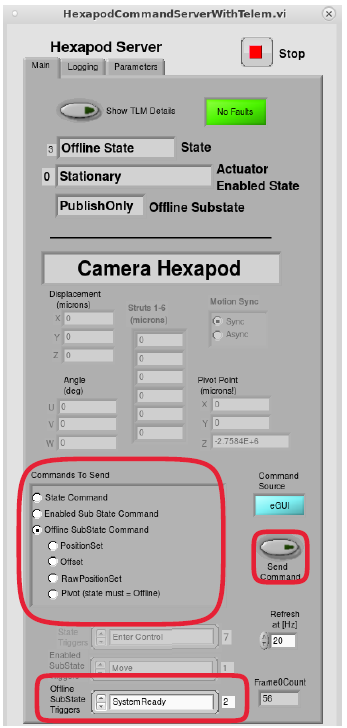
\includegraphics[width=1.79167in]{jira_imgs/1024.png}

}
\hdashrule[0.5ex]{\textwidth}{1pt}{3mm}
  Expected Result \\
{\footnotesize
The system transitions from the OfflineState/PublishOnly substate to the
OfflineState/AvailableState substate and the Command Source says
eGUI.\\[2\baselineskip]

}
\hdashrule[0.5ex]{\textwidth}{1pt}{3mm}
  Actual Result \\
{\footnotesize

}
\begin{tabular}{p{2cm}p{14cm}}
\toprule
Step 7 & Step Execution Status: \textbf{ Not Executed } \\ \hline
\end{tabular}
 Description \\
{\footnotesize
\textbf{Clear Errors}\\[2\baselineskip]Send a \textbf{clearErrors}
command so we can have a fresh start via CSC. Otherwise, you might have
to send the CSC to ENABLED twice.

}
\hdashrule[0.5ex]{\textwidth}{1pt}{3mm}
  Expected Result \\
{\footnotesize

}
\hdashrule[0.5ex]{\textwidth}{1pt}{3mm}
  Actual Result \\
{\footnotesize

}
\begin{tabular}{p{2cm}p{14cm}}
\toprule
Step 8 & Step Execution Status: \textbf{ Not Executed } \\ \hline
\end{tabular}
 Description \\
{\footnotesize
\textbf{SWITCHING TO DDS MODE}\\
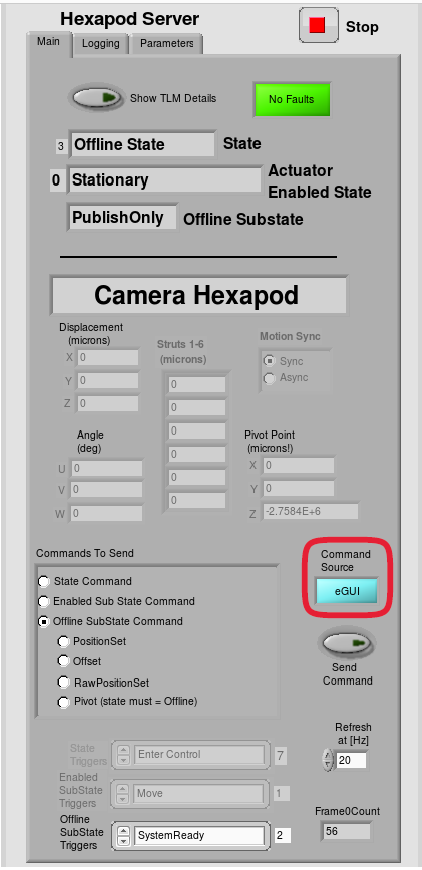
\includegraphics[width=1.68750in]{jira_imgs/1025.png}If the Command
Source does not show DDS, go to the \textbf{Parameters} tab, select
\textbf{DDS} under the \textbf{Command Source} and click the \textbf{Set
Cmd Source} button.\\
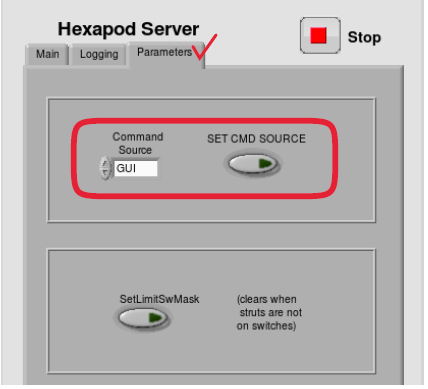
\includegraphics[width=2.34375in]{jira_imgs/1026.png}\textbf{Note:~If
the GUI is used after being set to DDS mode, the system will switch back
the Command Source to GUI and ignore any DDS commands. The Command
Source must show DDS in order to receive DDS commands.}

}
\hdashrule[0.5ex]{\textwidth}{1pt}{3mm}
  Expected Result \\
{\footnotesize
The system is capable of receiving/responding to DDS commands.\\
The \textbf{Command Source = DDS} green LED in the Telemetry Tab should
turn on.

}
\hdashrule[0.5ex]{\textwidth}{1pt}{3mm}
  Actual Result \\
{\footnotesize

}
\begin{tabular}{p{2cm}p{14cm}}
\toprule
Step 9 & Step Execution Status: \textbf{ Not Executed } \\ \hline
\end{tabular}
 Description \\
{\footnotesize
From any state send the CSC into OfflineState/AvailableState using the
EUI. Change the control at the EUI from EUI control to CSC
control.\\[2\baselineskip]Verify the Hexapod is commandable by DDS by
checking the EFD.

}
\hdashrule[0.5ex]{\textwidth}{1pt}{3mm}
  Expected Result \\
{\footnotesize
The \emph{MTHexapod\_logevent\_commandableByDDS} first publishes false
and then publishes true after the control has been returned to CSC
control.

}
\hdashrule[0.5ex]{\textwidth}{1pt}{3mm}
  Actual Result \\
{\footnotesize

}
\begin{tabular}{p{2cm}p{14cm}}
\toprule
Step 10 & Step Execution Status: \textbf{ Not Executed } \\ \hline
\end{tabular}
 Description \\
{\footnotesize
Verify the TCP/IP is connected to the low level controller.

}
\hdashrule[0.5ex]{\textwidth}{1pt}{3mm}
  Expected Result \\
{\footnotesize
The \emph{MTHexapod\_logevent\_connected} publishes true.

}
\hdashrule[0.5ex]{\textwidth}{1pt}{3mm}
  Actual Result \\
{\footnotesize

}
\begin{tabular}{p{2cm}p{14cm}}
\toprule
Step 11 & Step Execution Status: \textbf{ Not Executed } \\ \hline
\end{tabular}
 Description \\
{\footnotesize
Verify the \emph{MTHexapod\_logevent\_configuration} event is publishing
data to the EFD.

}
\hdashrule[0.5ex]{\textwidth}{1pt}{3mm}
  Test Data \\
 {\footnotesize
\textbf{Note:} This step is to verify the
\emph{MTHexapod\_logevent\_configuration} event is publishing initial
data. There will be steps later to verify that the event is published as
a result of updating values.

}
\hdashrule[0.5ex]{\textwidth}{1pt}{3mm}
  Expected Result \\
{\footnotesize
The \emph{MTHexapod\_logevent\_configuration} is publishing data.

}
\hdashrule[0.5ex]{\textwidth}{1pt}{3mm}
  Actual Result \\
{\footnotesize

}
\begin{tabular}{p{2cm}p{14cm}}
\toprule
Step 12 & Step Execution Status: \textbf{ Not Executed } \\ \hline
\end{tabular}
 Description \\
{\footnotesize
Verify the \emph{MTHexapod\_logevent\_interlock} event is unengaged and
publishing data to the EFD.

}
\hdashrule[0.5ex]{\textwidth}{1pt}{3mm}
  Expected Result \\
{\footnotesize
The \emph{MTHexapod\_logevent\_interlock} is publishing and shows no
safety interlock is engaged.

}
\hdashrule[0.5ex]{\textwidth}{1pt}{3mm}
  Actual Result \\
{\footnotesize

}
\begin{tabular}{p{2cm}p{14cm}}
\toprule
Step 13 & Step Execution Status: \textbf{ Not Executed } \\ \hline
\end{tabular}
 Description \\
{\footnotesize
Hit the E-stop.

}
\hdashrule[0.5ex]{\textwidth}{1pt}{3mm}
  Test Data \\
 {\footnotesize
\textbf{Note:~}This will mimic triggering an interlock signal from the
GIS.\\[2\baselineskip]

}
\hdashrule[0.5ex]{\textwidth}{1pt}{3mm}
  Expected Result \\
{\footnotesize
The \emph{MTHexapod\_logevent\_interlock~}publishes true.

}
\hdashrule[0.5ex]{\textwidth}{1pt}{3mm}
  Actual Result \\
{\footnotesize

}
\begin{tabular}{p{2cm}p{14cm}}
\toprule
Step 14 & Step Execution Status: \textbf{ Not Executed } \\ \hline
\end{tabular}
 Description \\
{\footnotesize
Reset the E-stop and clear the error:

\begin{itemize}
\tightlist
\item
  With the CSC in the Fault state, issue a \emph{standby} command via
  the CSC using the notebook.
\end{itemize}

}
\hdashrule[0.5ex]{\textwidth}{1pt}{3mm}
  Expected Result \\
{\footnotesize
The Hexapod and E-stop are reset and
\emph{MTHexapod\_logevent\_interlock~}publishes false.

}
\hdashrule[0.5ex]{\textwidth}{1pt}{3mm}
  Actual Result \\
{\footnotesize

}
\begin{tabular}{p{2cm}p{14cm}}
\toprule
Step 15 & Step Execution Status: \textbf{ Not Executed } \\ \hline
\end{tabular}
 Description \\
{\footnotesize
Verify that the thermal sensors are connected and producing telemetry
into the EFD. ``lsst.sal.ESS.temperature''

}
\hdashrule[0.5ex]{\textwidth}{1pt}{3mm}
  Expected Result \\
{\footnotesize
All actuator temperatures are published to the EFD.

}
\hdashrule[0.5ex]{\textwidth}{1pt}{3mm}
  Actual Result \\
{\footnotesize

}
\begin{tabular}{p{2cm}p{14cm}}
\toprule
Step 16 & Step Execution Status: \textbf{ Not Executed } \\ \hline
\end{tabular}
 Description \\
{\footnotesize
The following steps define what the Jupyter Notebook for this test case
implements. Executing the Jupyter notebook is the only actual command
and control step that needs to be executed.\\
Transition the state machine into \emph{disabledState~}to publish
telemetry

}
\hdashrule[0.5ex]{\textwidth}{1pt}{3mm}
  Expected Result \\
{\footnotesize
The Jupyter notebook controls the system to run through the steps below.

}
\hdashrule[0.5ex]{\textwidth}{1pt}{3mm}
  Actual Result \\
{\footnotesize

}
\begin{tabular}{p{2cm}p{14cm}}
\toprule
Step 17 & Step Execution Status: \textbf{ Not Executed } \\ \hline
\end{tabular}
 Description \\
{\footnotesize
Verify the \emph{MTHexapod\_actuators~}telemetry is being published to
the EFD with the following parameters:

\begin{itemize}
\tightlist
\item
  calibrated
\item
  raw
\item
  timestamp
\end{itemize}

}
\hdashrule[0.5ex]{\textwidth}{1pt}{3mm}
  Expected Result \\
{\footnotesize
The \emph{MTHexapod\_actuators} telemetry is being ingested into the
EFD.

}
\hdashrule[0.5ex]{\textwidth}{1pt}{3mm}
  Actual Result \\
{\footnotesize

}
\begin{tabular}{p{2cm}p{14cm}}
\toprule
Step 18 & Step Execution Status: \textbf{ Not Executed } \\ \hline
\end{tabular}
 Description \\
{\footnotesize
Verify the \emph{MTHexapod\_application~}data is being published to the
EFD with the following parameters:

\begin{itemize}
\tightlist
\item
  demand
\item
  position
\item
  error
\end{itemize}

}
\hdashrule[0.5ex]{\textwidth}{1pt}{3mm}
  Expected Result \\
{\footnotesize
The \emph{MTHexapod\_application} telemetry is being ingested into the
EFD.

}
\hdashrule[0.5ex]{\textwidth}{1pt}{3mm}
  Actual Result \\
{\footnotesize

}
\begin{tabular}{p{2cm}p{14cm}}
\toprule
Step 19 & Step Execution Status: \textbf{ Not Executed } \\ \hline
\end{tabular}
 Description \\
{\footnotesize
Verify the \emph{MTHexapod\_electrical~}data is being published to the
EFD with the following parameters:

\begin{itemize}
\tightlist
\item
  copleyStatusWordDrive
\item
  copleyLatchingFaultStatus
\item
  motorCurrent
\item
  busVoltage
\end{itemize}

}
\hdashrule[0.5ex]{\textwidth}{1pt}{3mm}
  Expected Result \\
{\footnotesize
The \emph{MTHexapod\_electrical} telemetry is being ingested into the
EFD.

}
\hdashrule[0.5ex]{\textwidth}{1pt}{3mm}
  Actual Result \\
{\footnotesize

}
\begin{tabular}{p{2cm}p{14cm}}
\toprule
Step 20 & Step Execution Status: \textbf{ Not Executed } \\ \hline
\end{tabular}
 Description \\
{\footnotesize
\textbf{{MOVE TEST}}\\
\textbf{Section 3.1.2 of the attached Software Acceptance Test
Procedure\\
Test Sequence \#1 - Synchronous Move Commands}\\
With the synchronous button enabled and in enabled/stationary state,
send a \emph{move} command of (500um, -500um, 200um, 0.01deg, -0.015deg,
0deg).

}
\hdashrule[0.5ex]{\textwidth}{1pt}{3mm}
  Expected Result \\
{\footnotesize
\begin{itemize}
\tightlist
\item
  The hexapod moves to (x= 500um,y= -500um, z=200um, u=0.01deg,
  v=-0.015deg, w=0deg)
\item
  Since the Hexapod is in synchronous mode, the actuators complete the
  move at nearly the same time.
\end{itemize}

}
\hdashrule[0.5ex]{\textwidth}{1pt}{3mm}
  Actual Result \\
{\footnotesize

}
\begin{tabular}{p{2cm}p{14cm}}
\toprule
Step 21 & Step Execution Status: \textbf{ Not Executed } \\ \hline
\end{tabular}
 Description \\
{\footnotesize
Record the corresponding DDS events that were generated.

}
\hdashrule[0.5ex]{\textwidth}{1pt}{3mm}
  Expected Result \\
{\footnotesize
\begin{itemize}
\tightlist
\item
  The controllerState.enabledSubstate goes to MOVING\_POINT\_TO\_POINT
  when the move begins and STATIONARY when the move ends.
\item
  An \emph{MTHexapod\_logevent\_inPosition} event is generated when the
  move is complete
\end{itemize}

}
\hdashrule[0.5ex]{\textwidth}{1pt}{3mm}
  Actual Result \\
{\footnotesize

}
\begin{tabular}{p{2cm}p{14cm}}
\toprule
Step 22 & Step Execution Status: \textbf{ Not Executed } \\ \hline
\end{tabular}
 Description \\
{\footnotesize
\textbf{Section 3.1.2 of the attached Software Acceptance Test
Procedure\\
Test Sequence \#5 - Stop Commands}\\
In the enabled/stationary state, send a \emph{move} command of (x=0um,
y=0um, z=5000um, u=0deg, v=0deg, w=0deg)

}
\hdashrule[0.5ex]{\textwidth}{1pt}{3mm}
  Expected Result \\
{\footnotesize
The hexapod begins to move.

}
\hdashrule[0.5ex]{\textwidth}{1pt}{3mm}
  Actual Result \\
{\footnotesize

}
\begin{tabular}{p{2cm}p{14cm}}
\toprule
Step 23 & Step Execution Status: \textbf{ Not Executed } \\ \hline
\end{tabular}
 Description \\
{\footnotesize
Wait 3s.

}
\hdashrule[0.5ex]{\textwidth}{1pt}{3mm}
  Expected Result \\
{\footnotesize
The hexapod is still moving.

}
\hdashrule[0.5ex]{\textwidth}{1pt}{3mm}
  Actual Result \\
{\footnotesize

}
\begin{tabular}{p{2cm}p{14cm}}
\toprule
Step 24 & Step Execution Status: \textbf{ Not Executed } \\ \hline
\end{tabular}
 Description \\
{\footnotesize
Send a \emph{stop} command.

}
\hdashrule[0.5ex]{\textwidth}{1pt}{3mm}
  Expected Result \\
{\footnotesize
The hexapod stops before reaching the previously commanded position

}
\hdashrule[0.5ex]{\textwidth}{1pt}{3mm}
  Actual Result \\
{\footnotesize

}
\begin{tabular}{p{2cm}p{14cm}}
\toprule
Step 25 & Step Execution Status: \textbf{ Not Executed } \\ \hline
\end{tabular}
 Description \\
{\footnotesize
Record the corresponding DDS events that were generated.

}
\hdashrule[0.5ex]{\textwidth}{1pt}{3mm}
  Expected Result \\
{\footnotesize
\begin{itemize}
\tightlist
\item
  The controllerState.enabledSubstate goes to CONTROLLED\_STOPPING when
  the stop is requested, then STATIONARY when the hexapod has halted.
\item
  No \emph{MTHexapod\_logevent\_inPosition} event is generated.
\end{itemize}

}
\hdashrule[0.5ex]{\textwidth}{1pt}{3mm}
  Actual Result \\
{\footnotesize

}
\begin{tabular}{p{2cm}p{14cm}}
\toprule
Step 26 & Step Execution Status: \textbf{ Not Executed } \\ \hline
\end{tabular}
 Description \\
{\footnotesize
\textbf{Test the ``setCompensationMode'' command.}\\[2\baselineskip]In
enabled/stationary state, send a \emph{move} command of (x=0um, y=0um,
z=800um, u=0deg, v=0deg, w=0deg)

}
\hdashrule[0.5ex]{\textwidth}{1pt}{3mm}
  Expected Result \\
{\footnotesize
The hexapod moves to the position (x=0um, y=0um, z=800um, u=0deg,
v=0deg, w=0deg) and, since we are moving in synchronous mode, the
actuators complete the move at nearly the same time.

}
\hdashrule[0.5ex]{\textwidth}{1pt}{3mm}
  Actual Result \\
{\footnotesize

}
\begin{tabular}{p{2cm}p{14cm}}
\toprule
Step 27 & Step Execution Status: \textbf{ Not Executed } \\ \hline
\end{tabular}
 Description \\
{\footnotesize
Ensure that MTMount publishes the telescope elevation angle and
MTRotator publishes the rotation angle of the rotator. Either as real
components or through controllers simulating the components.

}
\hdashrule[0.5ex]{\textwidth}{1pt}{3mm}
  Expected Result \\
{\footnotesize
Published telescope elevation and rotator angle.

}
\hdashrule[0.5ex]{\textwidth}{1pt}{3mm}
  Actual Result \\
{\footnotesize

}
\begin{tabular}{p{2cm}p{14cm}}
\toprule
Step 28 & Step Execution Status: \textbf{ Not Executed } \\ \hline
\end{tabular}
 Description \\
{\footnotesize
In enabled/stationary state, set \emph{setCompensationMode} command to
enable=True.

}
\hdashrule[0.5ex]{\textwidth}{1pt}{3mm}
  Expected Result \\
{\footnotesize
\begin{itemize}
\tightlist
\item
  The hexapod does not move and the
  ~\emph{MTHexapod\_logevent\_compensationMode} event appears as true in
  the EFD.
\item
  The \emph{MTHexapod\_logevent\_compensatedPosition} is also sent to
  the EFD.
\end{itemize}

}
\hdashrule[0.5ex]{\textwidth}{1pt}{3mm}
  Actual Result \\
{\footnotesize

}
\begin{tabular}{p{2cm}p{14cm}}
\toprule
Step 29 & Step Execution Status: \textbf{ Not Executed } \\ \hline
\end{tabular}
 Description \\
{\footnotesize
In enabled/stationary state, send a \emph{move} command of (0um, 0um,
800um, 0deg, 0deg, 0deg)

}
\hdashrule[0.5ex]{\textwidth}{1pt}{3mm}
  Expected Result \\
{\footnotesize
The hexapod moves to a slightly different position than (0um, 0um,
800um, 0deg, 0deg, 0deg) and, since we are moving in synchronous mode,
the actuators complete the move at nearly the same time.

}
\hdashrule[0.5ex]{\textwidth}{1pt}{3mm}
  Actual Result \\
{\footnotesize

}
\begin{tabular}{p{2cm}p{14cm}}
\toprule
Step 30 & Step Execution Status: \textbf{ Not Executed } \\ \hline
\end{tabular}
 Description \\
{\footnotesize
{Check if there are any different events between move with and without
setCompensationMode=True. Check the movement in the EFD use:\\
Compare \emph{MTHexapod\_logevent\_compensatedPosition} to
\emph{MTHexapod\_logevent\_uncompensatedPosition}}{\\
}

}
\hdashrule[0.5ex]{\textwidth}{1pt}{3mm}
  Expected Result \\
{\footnotesize
The changes are expected according to this table:\\
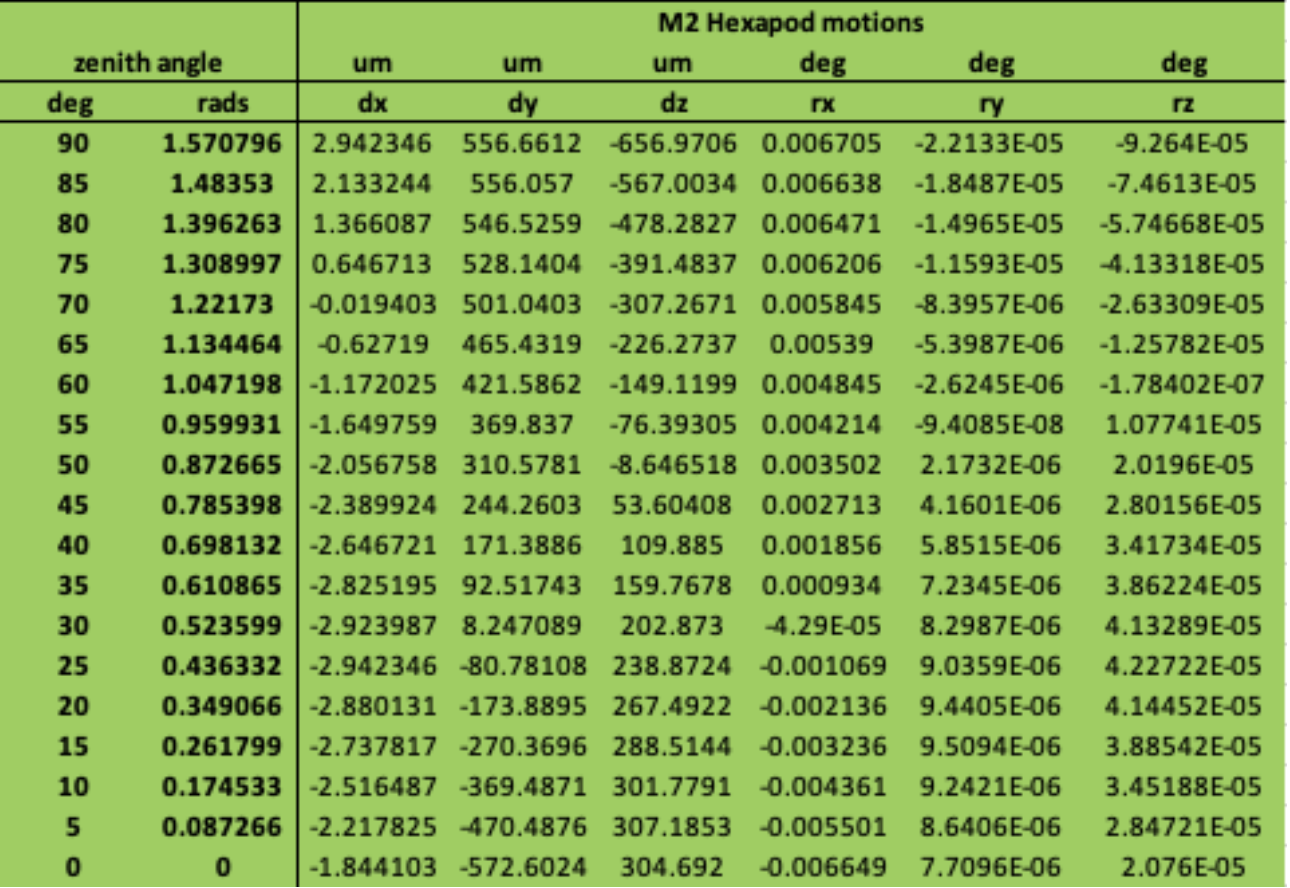
\includegraphics[width=3.12500in]{jira_imgs/1620.png}

}
\hdashrule[0.5ex]{\textwidth}{1pt}{3mm}
  Actual Result \\
{\footnotesize

}
\begin{tabular}{p{2cm}p{14cm}}
\toprule
Step 31 & Step Execution Status: \textbf{ Not Executed } \\ \hline
\end{tabular}
 Description \\
{\footnotesize
In enabled/stationary state, send again the same \emph{move} command of
(0um, 0um, 800um, 0deg, 0deg, 0deg)

}
\hdashrule[0.5ex]{\textwidth}{1pt}{3mm}
  Expected Result \\
{\footnotesize
The hexapod does not move since it stayed in compensationMode.

}
\hdashrule[0.5ex]{\textwidth}{1pt}{3mm}
  Actual Result \\
{\footnotesize

}
\begin{tabular}{p{2cm}p{14cm}}
\toprule
Step 32 & Step Execution Status: \textbf{ Not Executed } \\ \hline
\end{tabular}
 Description \\
{\footnotesize
{\textbf{OFFSET TEST}}\\
\textbf{Section 3.1.2 of the attached Software Acceptance Test
Procedure\\
Test Sequence \#4 - Synchronous Offset and Move Commands}\\
In enabled/stationary state, send a \emph{move} command of (x=500um,
y=800um, z=200um, u=0deg, v=0deg, w=0deg)

}
\hdashrule[0.5ex]{\textwidth}{1pt}{3mm}
  Test Data \\
 {\footnotesize


}
\hdashrule[0.5ex]{\textwidth}{1pt}{3mm}
  Expected Result \\
{\footnotesize
\begin{itemize}
\tightlist
\item
  The hexapod moves to (x=500um, y=800um, z=200um, u=0deg, v=0deg,
  w=0deg)
\item
  Since the Hexapod is in synchronous mode, the actuators complete the
  move at nearly the same time.
\end{itemize}

}
\hdashrule[0.5ex]{\textwidth}{1pt}{3mm}
  Actual Result \\
{\footnotesize

}
\begin{tabular}{p{2cm}p{14cm}}
\toprule
Step 33 & Step Execution Status: \textbf{ Not Executed } \\ \hline
\end{tabular}
 Description \\
{\footnotesize
In enabled/stationary state, send an \emph{offset} command of (0um, 0um,
500um, 0deg, 0deg, 0deg).

}
\hdashrule[0.5ex]{\textwidth}{1pt}{3mm}
  Expected Result \\
{\footnotesize
\begin{itemize}
\tightlist
\item
  The hexapod moves only 500um in Z from the previous position
\item
  The actuators complete the move at nearly the same time.
\item
  The \emph{MTHexapod\_logevent\_compensationOffset~}starts to publish
  data to the EFD based on the computed compensation offset and the
  input parameters provided.
\end{itemize}

}
\hdashrule[0.5ex]{\textwidth}{1pt}{3mm}
  Actual Result \\
{\footnotesize

}
\begin{tabular}{p{2cm}p{14cm}}
\toprule
Step 34 & Step Execution Status: \textbf{ Not Executed } \\ \hline
\end{tabular}
 Description \\
{\footnotesize
Record the corresponding DDS events that were generated.

}
\hdashrule[0.5ex]{\textwidth}{1pt}{3mm}
  Expected Result \\
{\footnotesize
\begin{itemize}
\tightlist
\item
  The controllerState.enabledSubstate goes to MOVING\_POINT\_TO\_POINT
  when the move begins and STATIONARY when the move ends
\item
  The \emph{MTHexapod\_logevent\_inPosition} event is True when the move
  finishes
\item
  The \emph{MTHexapod\_logevent\_inPosition} event is False when the
  enabledSubstate goes back to STATIONARY.
\end{itemize}

}
\hdashrule[0.5ex]{\textwidth}{1pt}{3mm}
  Actual Result \\
{\footnotesize

}
\begin{tabular}{p{2cm}p{14cm}}
\toprule
Step 35 & Step Execution Status: \textbf{ Not Executed } \\ \hline
\end{tabular}
 Description \\
{\footnotesize
\textbf{Section 3.1.2 of the attached Software Acceptance Test
Procedure\\
Test Sequence \#2 - setPivot and Move Commands}\\
In enabled/stationary state, send a \emph{move} command of
(x=2000um,y=-3500um,z=200um,u=0.01deg,v=-0.05deg, w=0.002deg,sync=true)

}
\hdashrule[0.5ex]{\textwidth}{1pt}{3mm}
  Test Data \\
 {\footnotesize
\textbf{Deviation:} Determine where the original pivot point is before
sending a \emph{setPivot} command of (0, 0, 0).\\
Record any offset commands necessary to test before sending the move
command.

}
\hdashrule[0.5ex]{\textwidth}{1pt}{3mm}
  Expected Result \\
{\footnotesize
The hexapod moves to the commanded position

}
\hdashrule[0.5ex]{\textwidth}{1pt}{3mm}
  Actual Result \\
{\footnotesize

}
\begin{tabular}{p{2cm}p{14cm}}
\toprule
Step 36 & Step Execution Status: \textbf{ Not Executed } \\ \hline
\end{tabular}
 Description \\
{\footnotesize
In the enabled/stationary state, send the \emph{setPivot} command of
(0,0,0).

}
\hdashrule[0.5ex]{\textwidth}{1pt}{3mm}
  Expected Result \\
{\footnotesize
\begin{itemize}
\tightlist
\item
  The actuator positions do not change but the hexapod position changes
  to account for the new pivot point.
\item
  The\emph{~MTHexapod\_logevent\_configuration} is updated.
\end{itemize}

}
\hdashrule[0.5ex]{\textwidth}{1pt}{3mm}
  Actual Result \\
{\footnotesize

}
\begin{tabular}{p{2cm}p{14cm}}
\toprule
Step 37 & Step Execution Status: \textbf{ Not Executed } \\ \hline
\end{tabular}
 Description \\
{\footnotesize
In the enabled/stationary state, send again the \emph{move} command of
(x=2000um, y=-3500um, z=200um, u=0.01deg, v=-0.05deg,
w=0.002deg,sync=true)

}
\hdashrule[0.5ex]{\textwidth}{1pt}{3mm}
  Test Data \\
 {\footnotesize
\textbf{Deviation}: ~Record any offset commands necessary to test before
sending the move command.

}
\hdashrule[0.5ex]{\textwidth}{1pt}{3mm}
  Expected Result \\
{\footnotesize
The hexapod doesn't move. Position values in the EFD appear different.

}
\hdashrule[0.5ex]{\textwidth}{1pt}{3mm}
  Actual Result \\
{\footnotesize

}
\begin{tabular}{p{2cm}p{14cm}}
\toprule
Step 38 & Step Execution Status: \textbf{ Not Executed } \\ \hline
\end{tabular}
 Description \\
{\footnotesize
\textbf{{CONFIGURE LIMITS TEST}}\\
\textbf{Section 3.1.2 of the attached Software Acceptance Test
Procedure\\
Test Sequence \#6 - configureLimits Command}\\
In enabled/stationary state, send a \emph{configureLimits} command of
(12000um, -1000um, 1000um, 0.1, -0.1, 0.05)

}
\hdashrule[0.5ex]{\textwidth}{1pt}{3mm}
  Expected Result \\
{\footnotesize
The command is rejected for being outside acceptable limits.

}
\hdashrule[0.5ex]{\textwidth}{1pt}{3mm}
  Actual Result \\
{\footnotesize

}
\begin{tabular}{p{2cm}p{14cm}}
\toprule
Step 39 & Step Execution Status: \textbf{ Not Executed } \\ \hline
\end{tabular}
 Description \\
{\footnotesize
In enabled/stationary state, send a \emph{configureLimits} command of
(1000um, -1000um, 1000um, 0.1, -0.1, 0.05)

}
\hdashrule[0.5ex]{\textwidth}{1pt}{3mm}
  Expected Result \\
{\footnotesize
The command is accepted and \emph{MTHexapod\_logevent\_configuration}
event is updated.

}
\hdashrule[0.5ex]{\textwidth}{1pt}{3mm}
  Actual Result \\
{\footnotesize

}
\begin{tabular}{p{2cm}p{14cm}}
\toprule
Step 40 & Step Execution Status: \textbf{ Not Executed } \\ \hline
\end{tabular}
 Description \\
{\footnotesize
In enabled/stationary state, send a \emph{move} command of (850um, 0um,
500um, 0deg, 0deg, 0deg)

}
\hdashrule[0.5ex]{\textwidth}{1pt}{3mm}
  Test Data \\
 {\footnotesize
\textbf{Note:~}This command can be any valid \emph{move} command within
the newly configured limits.

}
\hdashrule[0.5ex]{\textwidth}{1pt}{3mm}
  Expected Result \\
{\footnotesize
The command is accepted and the hexapod moves to the commanded position.

}
\hdashrule[0.5ex]{\textwidth}{1pt}{3mm}
  Actual Result \\
{\footnotesize

}
\begin{tabular}{p{2cm}p{14cm}}
\toprule
Step 41 & Step Execution Status: \textbf{ Not Executed } \\ \hline
\end{tabular}
 Description \\
{\footnotesize
In enabled/stationary state, send a \emph{move} command of (1200um, 0um,
200um, 0deg, 0deg, 0deg)

}
\hdashrule[0.5ex]{\textwidth}{1pt}{3mm}
  Test Data \\
 {\footnotesize
\textbf{Note:~}This command can be any invalid \emph{move} command
within the newly configured limits.

}
\hdashrule[0.5ex]{\textwidth}{1pt}{3mm}
  Expected Result \\
{\footnotesize
The command is rejected for being outside of range limits.

}
\hdashrule[0.5ex]{\textwidth}{1pt}{3mm}
  Actual Result \\
{\footnotesize

}
\begin{tabular}{p{2cm}p{14cm}}
\toprule
Step 42 & Step Execution Status: \textbf{ Not Executed } \\ \hline
\end{tabular}
 Description \\
{\footnotesize
In enabled/stationary state, send a \emph{move} command of (990um,
990um, 200um, 0deg, 0deg, 0deg)

}
\hdashrule[0.5ex]{\textwidth}{1pt}{3mm}
  Expected Result \\
{\footnotesize
The command is rejected for being outside of range limits.

}
\hdashrule[0.5ex]{\textwidth}{1pt}{3mm}
  Actual Result \\
{\footnotesize

}
\begin{tabular}{p{2cm}p{14cm}}
\toprule
Step 43 & Step Execution Status: \textbf{ Not Executed } \\ \hline
\end{tabular}
 Description \\
{\footnotesize
In enabled/stationary state, send a \emph{move} command of (500um,
500um, 200um, 0deg, 0.1 deg, 0.01deg)

}
\hdashrule[0.5ex]{\textwidth}{1pt}{3mm}
  Expected Result \\
{\footnotesize
The command is accepted and moves to the commanded position.

}
\hdashrule[0.5ex]{\textwidth}{1pt}{3mm}
  Actual Result \\
{\footnotesize

}
\begin{tabular}{p{2cm}p{14cm}}
\toprule
Step 44 & Step Execution Status: \textbf{ Not Executed } \\ \hline
\end{tabular}
 Description \\
{\footnotesize
Record the DDS events that were generated.

}
\hdashrule[0.5ex]{\textwidth}{1pt}{3mm}
  Expected Result \\
{\footnotesize
The change is reflected in the \emph{MTHexapod\_logevent\_configuration}
event and the EUI.

}
\hdashrule[0.5ex]{\textwidth}{1pt}{3mm}
  Actual Result \\
{\footnotesize

}
\begin{tabular}{p{2cm}p{14cm}}
\toprule
Step 45 & Step Execution Status: \textbf{ Not Executed } \\ \hline
\end{tabular}
 Description \\
{\footnotesize
{\textbf{CONFIGURE ACCELERATION TEST}}\\
\textbf{Section 3.1.2 of the attached Software Acceptance Test
Procedure\\
Test Sequence \#7 - configureAcceleration Command}\\
In enabled/stationary state, at a position of (0, 0, 0, 0, 0, 0) with
the velocity and acceleration values set to their nominal values, send a
\emph{move} command of (0um, 0um, 4900um, 0 deg, 0 deg, 0 deg, s).

}
\hdashrule[0.5ex]{\textwidth}{1pt}{3mm}
  Expected Result \\
{\footnotesize
The move takes approximately 9 seconds to complete.

}
\hdashrule[0.5ex]{\textwidth}{1pt}{3mm}
  Actual Result \\
{\footnotesize

}
\begin{tabular}{p{2cm}p{14cm}}
\toprule
Step 46 & Step Execution Status: \textbf{ Not Executed } \\ \hline
\end{tabular}
 Description \\
{\footnotesize
Send a \emph{configureAcceleration} command of 1000.

}
\hdashrule[0.5ex]{\textwidth}{1pt}{3mm}
  Expected Result \\
{\footnotesize
~Confirm command is rejected for being outside of acceptable limits.

}
\hdashrule[0.5ex]{\textwidth}{1pt}{3mm}
  Actual Result \\
{\footnotesize

}
\begin{tabular}{p{2cm}p{14cm}}
\toprule
Step 47 & Step Execution Status: \textbf{ Not Executed } \\ \hline
\end{tabular}
 Description \\
{\footnotesize
Send a \emph{configureAcceleration} command of 100.

}
\hdashrule[0.5ex]{\textwidth}{1pt}{3mm}
  Expected Result \\
{\footnotesize
The command is accepted.~

}
\hdashrule[0.5ex]{\textwidth}{1pt}{3mm}
  Actual Result \\
{\footnotesize

}
\begin{tabular}{p{2cm}p{14cm}}
\toprule
Step 48 & Step Execution Status: \textbf{ Not Executed } \\ \hline
\end{tabular}
 Description \\
{\footnotesize
In enabled/stationary state, send a \emph{move} command of (0um, 0um,
0um, 0 deg, 0 deg, 0 deg, s).

}
\hdashrule[0.5ex]{\textwidth}{1pt}{3mm}
  Expected Result \\
{\footnotesize
It takes approximately 13 seconds to complete the commanded move with
the reduced acceleration value.

}
\hdashrule[0.5ex]{\textwidth}{1pt}{3mm}
  Actual Result \\
{\footnotesize

}
\begin{tabular}{p{2cm}p{14cm}}
\toprule
Step 49 & Step Execution Status: \textbf{ Not Executed } \\ \hline
\end{tabular}
 Description \\
{\footnotesize
Send a \emph{configureAcceleration} command of 500 to return the
acceleration limit to its nominal value.

}
\hdashrule[0.5ex]{\textwidth}{1pt}{3mm}
  Expected Result \\
{\footnotesize
The command is accepted.

}
\hdashrule[0.5ex]{\textwidth}{1pt}{3mm}
  Actual Result \\
{\footnotesize

}
\begin{tabular}{p{2cm}p{14cm}}
\toprule
Step 50 & Step Execution Status: \textbf{ Not Executed } \\ \hline
\end{tabular}
 Description \\
{\footnotesize
Record the corresponding DDS events that were generated.

}
\hdashrule[0.5ex]{\textwidth}{1pt}{3mm}
  Expected Result \\
{\footnotesize
The change is reflected in the \emph{MTHexapod\_logevent\_configuration}
event and the EUI.

}
\hdashrule[0.5ex]{\textwidth}{1pt}{3mm}
  Actual Result \\
{\footnotesize

}
\begin{tabular}{p{2cm}p{14cm}}
\toprule
Step 51 & Step Execution Status: \textbf{ Not Executed } \\ \hline
\end{tabular}
 Description \\
{\footnotesize
\textbf{{CONFIGURE VELOCITY TEST}}\\
\textbf{Section 3.1.2 of the attached Software Acceptance Test
Procedure\\
Test Sequence \#8 - configureVelocity Command}\\
In enabled/stationary state, at a position of (0, 0, 0, 0, 0, 0), send a
\emph{configureVelocity} command of (10000, .01, 100, .01).

}
\hdashrule[0.5ex]{\textwidth}{1pt}{3mm}
  Expected Result \\
{\footnotesize
This command is rejected for being outside of acceptable limits.

}
\hdashrule[0.5ex]{\textwidth}{1pt}{3mm}
  Actual Result \\
{\footnotesize

}
\begin{tabular}{p{2cm}p{14cm}}
\toprule
Step 52 & Step Execution Status: \textbf{ Not Executed } \\ \hline
\end{tabular}
 Description \\
{\footnotesize
In enabled/stationary state, send a \emph{configureVelocity} command of
(100, .01, 200, .01).

}
\hdashrule[0.5ex]{\textwidth}{1pt}{3mm}
  Expected Result \\
{\footnotesize
This command is accepted.

}
\hdashrule[0.5ex]{\textwidth}{1pt}{3mm}
  Actual Result \\
{\footnotesize

}
\begin{tabular}{p{2cm}p{14cm}}
\toprule
Step 53 & Step Execution Status: \textbf{ Not Executed } \\ \hline
\end{tabular}
 Description \\
{\footnotesize
In enabled/stationary state, send a \emph{move} command of (0, 0,
2000um, 0 deg, 0 deg, 0 deg).

}
\hdashrule[0.5ex]{\textwidth}{1pt}{3mm}
  Expected Result \\
{\footnotesize
It takes approximately 20 seconds to complete the commanded move.

}
\hdashrule[0.5ex]{\textwidth}{1pt}{3mm}
  Actual Result \\
{\footnotesize

}
\begin{tabular}{p{2cm}p{14cm}}
\toprule
Step 54 & Step Execution Status: \textbf{ Not Executed } \\ \hline
\end{tabular}
 Description \\
{\footnotesize
In enabled/stationary state, send a \emph{configureVelocity} command of
(100, .01, 100, .01).

}
\hdashrule[0.5ex]{\textwidth}{1pt}{3mm}
  Expected Result \\
{\footnotesize
This command is accepted.

}
\hdashrule[0.5ex]{\textwidth}{1pt}{3mm}
  Actual Result \\
{\footnotesize

}
\begin{tabular}{p{2cm}p{14cm}}
\toprule
Step 55 & Step Execution Status: \textbf{ Not Executed } \\ \hline
\end{tabular}
 Description \\
{\footnotesize
In enabled/stationary state, send an \emph{offset} command of (0, 0,
2000um, 0 deg, 0 deg, 0 deg).

}
\hdashrule[0.5ex]{\textwidth}{1pt}{3mm}
  Expected Result \\
{\footnotesize
This command is accepted

}
\hdashrule[0.5ex]{\textwidth}{1pt}{3mm}
  Actual Result \\
{\footnotesize

}
\begin{tabular}{p{2cm}p{14cm}}
\toprule
Step 56 & Step Execution Status: \textbf{ Not Executed } \\ \hline
\end{tabular}
 Description \\
{\footnotesize
Send a \emph{move} command.

}
\hdashrule[0.5ex]{\textwidth}{1pt}{3mm}
  Expected Result \\
{\footnotesize
It takes approximately 40 seconds to complete the commanded move.

}
\hdashrule[0.5ex]{\textwidth}{1pt}{3mm}
  Actual Result \\
{\footnotesize

}
\begin{tabular}{p{2cm}p{14cm}}
\toprule
Step 57 & Step Execution Status: \textbf{ Not Executed } \\ \hline
\end{tabular}
 Description \\
{\footnotesize
Record the corresponding DDS events that were generated:

}
\hdashrule[0.5ex]{\textwidth}{1pt}{3mm}
  Expected Result \\
{\footnotesize
The change is reflected in the \emph{MTHexapod\_logevent\_configuration}
event and the EUI.

}
\hdashrule[0.5ex]{\textwidth}{1pt}{3mm}
  Actual Result \\
{\footnotesize

}
\begin{tabular}{p{2cm}p{14cm}}
\toprule
Step 58 & Step Execution Status: \textbf{ Not Executed } \\ \hline
\end{tabular}
 Description \\
{\footnotesize
\textbf{Section 3.3.2 of the attached Software Acceptance Test Procedure
Hexapod Action on State Commands}\\
The state machine is a standbyState entry state machine.\\
Transition the state machine into offlineState/publishOnly state.\\
In the offlineState/publishOnly state, send all commands

}
\hdashrule[0.5ex]{\textwidth}{1pt}{3mm}
  Test Data \\
 {\footnotesize
{\textbf{Note:} This section utilizes the commands defined in LSE-209}

}
\hdashrule[0.5ex]{\textwidth}{1pt}{3mm}
  Expected Result \\
{\footnotesize
There is no change and command is rejected.

}
\hdashrule[0.5ex]{\textwidth}{1pt}{3mm}
  Actual Result \\
{\footnotesize

}
\begin{tabular}{p{2cm}p{14cm}}
\toprule
Step 59 & Step Execution Status: \textbf{ Not Executed } \\ \hline
\end{tabular}
 Description \\
{\footnotesize
Transition the state machine into offlineState/Available state.\\
In the offlineState/Available state, send an enterControl command.

}
\hdashrule[0.5ex]{\textwidth}{1pt}{3mm}
  Expected Result \\
{\footnotesize
The system enters the standbyState.

}
\hdashrule[0.5ex]{\textwidth}{1pt}{3mm}
  Actual Result \\
{\footnotesize

}
\begin{tabular}{p{2cm}p{14cm}}
\toprule
Step 60 & Step Execution Status: \textbf{ Not Executed } \\ \hline
\end{tabular}
 Description \\
{\footnotesize
In the \textbf{standbyState,} send any command except start or
exitControl

}
\hdashrule[0.5ex]{\textwidth}{1pt}{3mm}
  Expected Result \\
{\footnotesize
There is no change and command is rejected.

}
\hdashrule[0.5ex]{\textwidth}{1pt}{3mm}
  Actual Result \\
{\footnotesize

}
\begin{tabular}{p{2cm}p{14cm}}
\toprule
Step 61 & Step Execution Status: \textbf{ Not Executed } \\ \hline
\end{tabular}
 Description \\
{\footnotesize
In the Standby state, send an exitControl command.

}
\hdashrule[0.5ex]{\textwidth}{1pt}{3mm}
  Expected Result \\
{\footnotesize
The system transitions into the Offline/Available state.

}
\hdashrule[0.5ex]{\textwidth}{1pt}{3mm}
  Actual Result \\
{\footnotesize

}
\begin{tabular}{p{2cm}p{14cm}}
\toprule
Step 62 & Step Execution Status: \textbf{ Not Executed } \\ \hline
\end{tabular}
 Description \\
{\footnotesize
Transition the state machine into standbyState.\\
In the Standby state, send a start command.

}
\hdashrule[0.5ex]{\textwidth}{1pt}{3mm}
  Expected Result \\
{\footnotesize
The system transitions into the disabledState.

}
\hdashrule[0.5ex]{\textwidth}{1pt}{3mm}
  Actual Result \\
{\footnotesize

}
\begin{tabular}{p{2cm}p{14cm}}
\toprule
Step 63 & Step Execution Status: \textbf{ Not Executed } \\ \hline
\end{tabular}
 Description \\
{\footnotesize
In the Disabled state, send any command except for the enabled or
standby command.

}
\hdashrule[0.5ex]{\textwidth}{1pt}{3mm}
  Expected Result \\
{\footnotesize
There is no change and the command is rejected.

}
\hdashrule[0.5ex]{\textwidth}{1pt}{3mm}
  Actual Result \\
{\footnotesize

}
\begin{tabular}{p{2cm}p{14cm}}
\toprule
Step 64 & Step Execution Status: \textbf{ Not Executed } \\ \hline
\end{tabular}
 Description \\
{\footnotesize
In the Disabled state, send the standby command.

}
\hdashrule[0.5ex]{\textwidth}{1pt}{3mm}
  Expected Result \\
{\footnotesize
The system transitions into the Standby state.

}
\hdashrule[0.5ex]{\textwidth}{1pt}{3mm}
  Actual Result \\
{\footnotesize

}
\begin{tabular}{p{2cm}p{14cm}}
\toprule
Step 65 & Step Execution Status: \textbf{ Not Executed } \\ \hline
\end{tabular}
 Description \\
{\footnotesize
Transition the state machine into disabledState\\
In the disabledState, send the ENABLE command.

}
\hdashrule[0.5ex]{\textwidth}{1pt}{3mm}
  Expected Result \\
{\footnotesize
The system transitions into the Enabled/Stationary state.

}
\hdashrule[0.5ex]{\textwidth}{1pt}{3mm}
  Actual Result \\
{\footnotesize

}
\begin{tabular}{p{2cm}p{14cm}}
\toprule
Step 66 & Step Execution Status: \textbf{ Not Executed } \\ \hline
\end{tabular}
 Description \\
{\footnotesize
In the Enabled/Stationary state, send either the enterControl command,
exitControl command, start command, clearError command, or enable
command.

}
\hdashrule[0.5ex]{\textwidth}{1pt}{3mm}
  Expected Result \\
{\footnotesize
There is no change and command is rejected.

}
\hdashrule[0.5ex]{\textwidth}{1pt}{3mm}
  Actual Result \\
{\footnotesize

}
\begin{tabular}{p{2cm}p{14cm}}
\toprule
Step 67 & Step Execution Status: \textbf{ Not Executed } \\ \hline
\end{tabular}
 Description \\
{\footnotesize
In the Enabled/Stationary state, send a disable command.

}
\hdashrule[0.5ex]{\textwidth}{1pt}{3mm}
  Expected Result \\
{\footnotesize
The system transitions into Disabled state.

}
\hdashrule[0.5ex]{\textwidth}{1pt}{3mm}
  Actual Result \\
{\footnotesize

}
\begin{tabular}{p{2cm}p{14cm}}
\toprule
Step 68 & Step Execution Status: \textbf{ Not Executed } \\ \hline
\end{tabular}
 Description \\
{\footnotesize
In the Fault state, send any command.

}
\hdashrule[0.5ex]{\textwidth}{1pt}{3mm}
  Expected Result \\
{\footnotesize
The state machine transitions into the commanded state.

}
\hdashrule[0.5ex]{\textwidth}{1pt}{3mm}
  Actual Result \\
{\footnotesize

}
\begin{tabular}{p{2cm}p{14cm}}
\toprule
Step 69 & Step Execution Status: \textbf{ Not Executed } \\ \hline
\end{tabular}
 Description \\
{\footnotesize
\textbf{Section 4 of the attached Software Acceptance Test Procedure}\\
In the Enabled/Stationary state, unplug a motor encoder cable for one of
the actuators.\textbf{}\\

}
\hdashrule[0.5ex]{\textwidth}{1pt}{3mm}
  Test Data \\
 {\footnotesize


}
\hdashrule[0.5ex]{\textwidth}{1pt}{3mm}
  Expected Result \\
{\footnotesize
A Drive Fault error event is created and the system transitions to Fault
state.

}
\hdashrule[0.5ex]{\textwidth}{1pt}{3mm}
  Actual Result \\
{\footnotesize

}
\begin{tabular}{p{2cm}p{14cm}}
\toprule
Step 70 & Step Execution Status: \textbf{ Not Executed } \\ \hline
\end{tabular}
 Description \\
{\footnotesize
In the Enabled/Stationary state, unplug a linear encoder cable for one
of the actuators.

}
\hdashrule[0.5ex]{\textwidth}{1pt}{3mm}
  Expected Result \\
{\footnotesize
A Drive Fault error event is created and the system transitions to Fault
state.

}
\hdashrule[0.5ex]{\textwidth}{1pt}{3mm}
  Actual Result \\
{\footnotesize

}
\begin{tabular}{p{2cm}p{14cm}}
\toprule
Step 71 & Step Execution Status: \textbf{ Not Executed } \\ \hline
\end{tabular}
 Description \\
{\footnotesize
Unplug a motor power cable from one of the actuators and command a Move.

}
\hdashrule[0.5ex]{\textwidth}{1pt}{3mm}
  Expected Result \\
{\footnotesize
A Following Error event is created and the system transitions to Fault
state.

}
\hdashrule[0.5ex]{\textwidth}{1pt}{3mm}
  Actual Result \\
{\footnotesize

}
\begin{tabular}{p{2cm}p{14cm}}
\toprule
Step 72 & Step Execution Status: \textbf{ Not Executed } \\ \hline
\end{tabular}
 Description \\
{\footnotesize
Activate an extension limit switch on one of the actuators by removing
the limit switch cover and manually tripping.

}
\hdashrule[0.5ex]{\textwidth}{1pt}{3mm}
  Expected Result \\
{\footnotesize
An Extended Limit Switch error event is created and the system
transitions into Fault state.

}
\hdashrule[0.5ex]{\textwidth}{1pt}{3mm}
  Actual Result \\
{\footnotesize

}
\begin{tabular}{p{2cm}p{14cm}}
\toprule
Step 73 & Step Execution Status: \textbf{ Not Executed } \\ \hline
\end{tabular}
 Description \\
{\footnotesize
Activate a retraction limit switch on one of the actuators by removing
the limit switch cover and manually tripping.

}
\hdashrule[0.5ex]{\textwidth}{1pt}{3mm}
  Expected Result \\
{\footnotesize
A Retracted Limit Switch error event is created and the system
transitions into Fault state.

}
\hdashrule[0.5ex]{\textwidth}{1pt}{3mm}
  Actual Result \\
{\footnotesize

}
\begin{tabular}{p{2cm}p{14cm}}
\toprule
Step 74 & Step Execution Status: \textbf{ Not Executed } \\ \hline
\end{tabular}
 Description \\
{\footnotesize
Unplug the Ethercat cable between the control PC and the first Copley
XE2 drive.

}
\hdashrule[0.5ex]{\textwidth}{1pt}{3mm}
  Expected Result \\
{\footnotesize
An Ethercat Lost event is created and the system transitions to Fault
state.

}
\hdashrule[0.5ex]{\textwidth}{1pt}{3mm}
  Actual Result \\
{\footnotesize

}

\paragraph{ LVV-T1615 - Integration of M2 with SAL }\mbox{}\\

Version \textbf{2}.
Open  \href{https://jira.lsstcorp.org/secure/Tests.jspa#/testCase/LVV-T1615}{\textit{ LVV-T1615 } }
test case in Jira.

The objective of this test case is to verify the software requirements
of the M2 cell, as defined in \citeds{LTS-146} and \citeds{LTS-162}, utilizing the updated
M2 CSC (SAL). The software requirements were previously verified during
the test campaign by the vendor, but have since been updated per
CR-0202. This test case will exercise the functionality of the M2 CSC
and meets the following criteria:

\begin{itemize}
\tightlist
\item
  Only requires the most current version of SAL
\item
  Only requires the M2 surrogate to be loaded on the cell
\item
  Only requires the use of the DDS
\item
  Does \textbf{NOT} require the M2 to be integrated with the Interlock
  system
\end{itemize}

\textbf{ Preconditions}:\\


Execution status: {\bf Fail }

Final comment:\\The software is frozen at this moment for the installation of ComCam on
the TMA.\\
This execution uses Labview software. Mayor rewriting and translation to
python and C is in progress.\\
Test steps that have passed in this execution and are subject to changes
in the future are marked with ``initial pass''.\\
Some of the steps are not executed because the functionality will only
be implemented with the software rewrite.


Detailed steps results:

\begin{tabular}{p{2cm}p{14cm}}
\toprule
Step 1 & Step Execution Status: \textbf{ Pass } \\ \hline
\end{tabular}
 Description \\
{\footnotesize
\textbf{M2 DDS Startup Procedure}

}
\hdashrule[0.5ex]{\textwidth}{1pt}{3mm}
  Expected Result \\
{\footnotesize

}
\hdashrule[0.5ex]{\textwidth}{1pt}{3mm}
  Actual Result \\
{\footnotesize
Nothing to be done here.

}
\begin{tabular}{p{2cm}p{14cm}}
\toprule
Step 2 & Step Execution Status: \textbf{ Pass } \\ \hline
\end{tabular}
 Description \\
{\footnotesize
\textbf{Connect to~https://ls.st/hexrot-vm01}\\[2\baselineskip]Make sure
that you have an IPA account and that your username is part of the
\textbf{saluser} group.\\[2\baselineskip]Access
\textbf{https://ls.st/hexrot-vm01} using a browser (Firefox
recommended).\\[2\baselineskip]Log in with your account and open a
terminal.

}
\hdashrule[0.5ex]{\textwidth}{1pt}{3mm}
  Expected Result \\
{\footnotesize
You will be connected using the browser via TeamViewer. Other users
might be watching your session.

}
\hdashrule[0.5ex]{\textwidth}{1pt}{3mm}
  Actual Result \\
{\footnotesize
Done.~

}
\begin{tabular}{p{2cm}p{14cm}}
\toprule
Step 3 & Step Execution Status: \textbf{ Pass } \\ \hline
\end{tabular}
 Description \\
{\footnotesize
\textbf{Start MTM2 EUI}\\[2\baselineskip]Using the terminal, navigate to
the \textbf{/rubin/mtm2/build} folder and execute \textbf{runM2Cntlr}.\\
Use the example code below to check if there is another session before
starting your own.\\
If there is another session running, it is recommended that you contact
the user and ask them to close it.

}
\hdashrule[0.5ex]{\textwidth}{1pt}{3mm}
  Example Code \\
{\footnotesize
\$~~\texttt{ps} \texttt{-awx\ \textbar{}~}\texttt{grep}
\texttt{runM2Cntlr~\ \#\ Check\ existing\ session\ running}\\
\texttt{\$\ cd\ /rubin/mtm2/build}\\
\texttt{\$\ ./runM2Cntlr\ \#\ run\ the\ MtM2\ EUI~}

}
\hdashrule[0.5ex]{\textwidth}{1pt}{3mm}
  Expected Result \\
{\footnotesize
The M2 EUI should start and should be in Remote mode.\\
The state transitions should be done automatically when M2 EUI starts.

}
\hdashrule[0.5ex]{\textwidth}{1pt}{3mm}
  Actual Result \\
{\footnotesize
M2 is disconnected from the GIS.\\
Before moving forward, we tried to send M2 EUI to ENABLED locally.\\
It worked as expected.\\[2\baselineskip]There are a few warnings
though:\\
- Monitoring ILC read error\\
- Stale data warning\\[2\baselineskip]These are known issues and they
will be addressed during the code translation from LabView to C++.\\
This translation is not on our side. SLAC will do it (John
Gates).\\[2\baselineskip]We also closed the loop and could see the
errors in the axial forces going to small (\textless{} 0.3 N)
numbers.\\[2\baselineskip]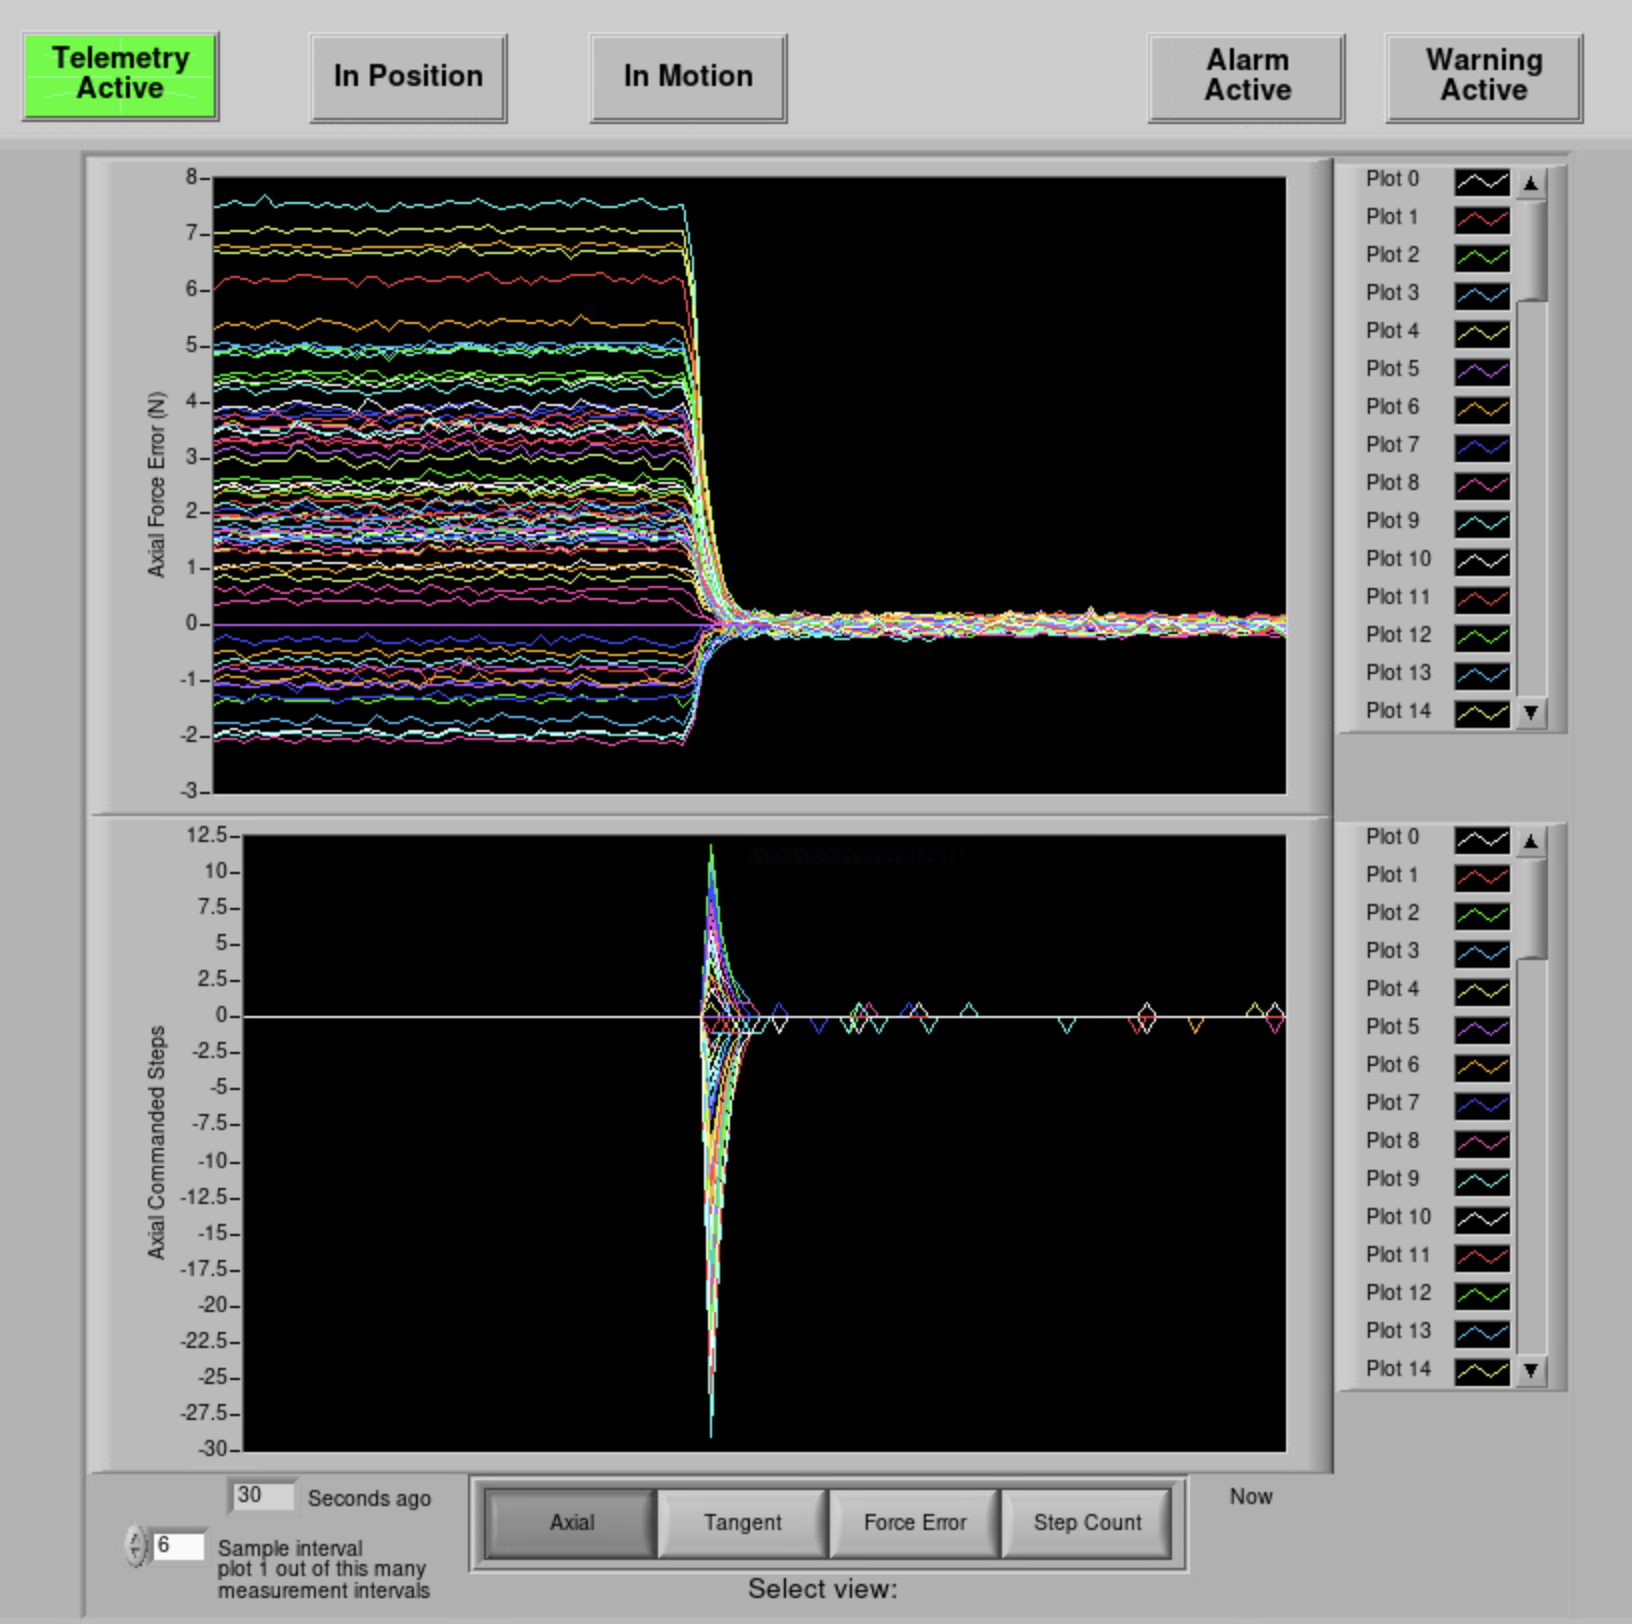
\includegraphics[width=3.12500in]{jira_imgs/2491.png}\\
Now that we confirmed that M2 EUI could go to CLOSED LOOP, we can open
the loop again.\\
Once the loop is open, we can send M2 EUI to STANDBY and set it to
remote control.\\
Now we can control M2 via SAL.

}
\begin{tabular}{p{2cm}p{14cm}}
\toprule
Step 4 & Step Execution Status: \textbf{ Not Executed } \\ \hline
\end{tabular}
 Description \\
{\footnotesize
Using the M2 EUI, return the M2 to open loop and send the M2 to STANDBY

}
\hdashrule[0.5ex]{\textwidth}{1pt}{3mm}
  Expected Result \\
{\footnotesize
The M2 is in STANDBY

}
\hdashrule[0.5ex]{\textwidth}{1pt}{3mm}
  Actual Result \\
{\footnotesize

}
\begin{tabular}{p{2cm}p{14cm}}
\toprule
Step 5 & Step Execution Status: \textbf{ Pass } \\ \hline
\end{tabular}
 Description \\
{\footnotesize
Use the chronograf to verify data is being published to the EFD.

}
\hdashrule[0.5ex]{\textwidth}{1pt}{3mm}
  Test Data \\
 {\footnotesize
Note: If no data is being published to the EFD, contact either Tiago
Ribeiro or Angelo Fausti for help.

}
\hdashrule[0.5ex]{\textwidth}{1pt}{3mm}
  Expected Result \\
{\footnotesize
{Data is being published to the EFD.}\\[2\baselineskip]{If M2 is not
ENABLED, only some telemetry will be published to the EFD.~}\\
All the telemetry should show up when M2 is in ENABLED.

}
\hdashrule[0.5ex]{\textwidth}{1pt}{3mm}
  Actual Result \\
{\footnotesize
We have some data being published to the EFD.\\
It makes sense that we do not have all the telemetry since M2 is now in
STANDBY.

}
\begin{tabular}{p{2cm}p{14cm}}
\toprule
Step 6 & Step Execution Status: \textbf{ Initial Pass } \\ \hline
\end{tabular}
 Description \\
{\footnotesize
\textbf{REMOTE CONTROL}\\[2\baselineskip]The system should be in the
remote control by default.\\
The initial substate is Offline/PublishOnly.\\
If the system passes all the checking, it will transition to
Offline/AvailableState substate.\\
You can see the state information
here:\\[2\baselineskip]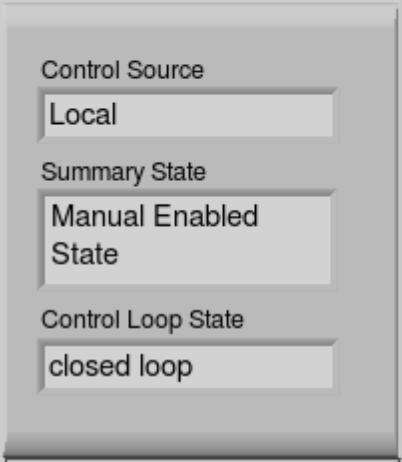
\includegraphics[width=1.30208in]{jira_imgs/1490.png}\textbf{\\
}

}
\hdashrule[0.5ex]{\textwidth}{1pt}{3mm}
  Test Data \\
 {\footnotesize
Note: The M2 control system was updated so that it could be transitioned
from Offline/PublishOnly to Offline/AvailableState as discussed
in~\href{https://jira.lsstcorp.org/browse/DM-2729}{DM-27291}

}
\hdashrule[0.5ex]{\textwidth}{1pt}{3mm}
  Expected Result \\
{\footnotesize
The system is under the remote control and in Offline/AvailableState
substate.\\[2\baselineskip]All the other state/substate transitions are
done via CSC.

}
\hdashrule[0.5ex]{\textwidth}{1pt}{3mm}
  Actual Result \\
{\footnotesize
The M2 EUI shows that it could transition to AvailableState in the Log
window. However, it might take a long time to find the message.\\
The easiest way of checking if it could is checking the
logs:\\[2\baselineskip]\$ cd /rubin/mtm2/logs\\
\$ cat \$LOG\_OF\_THE\_DAY \textbar{} grep -i available\\
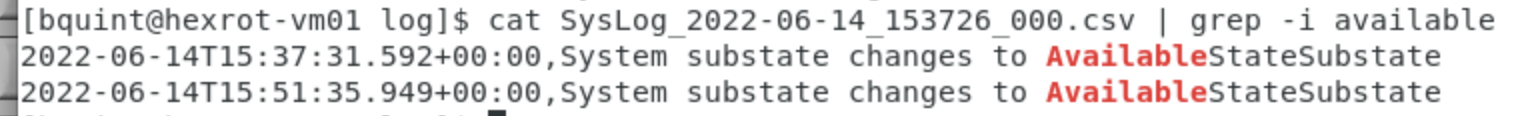
\includegraphics[width=3.12500in]{jira_imgs/2492.png}

}
\begin{tabular}{p{2cm}p{14cm}}
\toprule
Step 7 & Step Execution Status: \textbf{ Initial Pass } \\ \hline
\end{tabular}
 Description \\
{\footnotesize
Transition the MTM2 CSC into DISABLED state either through LOVE or
through Jupyter Notebook.~

}
\hdashrule[0.5ex]{\textwidth}{1pt}{3mm}
  Test Data \\
 {\footnotesize
\textbf{Note:~}When transitioning through LOVE, use the default
configuration.\\
If transitioning through the use of a Jupyter Notebook, you must start
the Daemon first.

}
\hdashrule[0.5ex]{\textwidth}{1pt}{3mm}
  Expected Result \\
{\footnotesize
The MTM2 CSC transitions into the DISABLED state

}
\hdashrule[0.5ex]{\textwidth}{1pt}{3mm}
  Actual Result \\
{\footnotesize
We first transition the mtm2 CSC to DISABLED. I did the transition via
LOVE and it worked fine.\\
LOVE showed that mtm2 has hearbeats. Chronograph does not show
heartbeats.

}
\begin{tabular}{p{2cm}p{14cm}}
\toprule
Step 8 & Step Execution Status: \textbf{ Initial Pass } \\ \hline
\end{tabular}
 Description \\
{\footnotesize
Verify the M2 is commandable by DDS by checking the EFD.~

}
\hdashrule[0.5ex]{\textwidth}{1pt}{3mm}
  Expected Result \\
{\footnotesize
The \emph{MTM2\_logevent\_commandableByDDS} publishes true.

}
\hdashrule[0.5ex]{\textwidth}{1pt}{3mm}
  Actual Result \\
{\footnotesize
We could not confirm this event on Chronograph but we could retrieve its
value using Notebooks.\\[2\baselineskip]\textbf{m2\_commandable\_by\_dds
= mtcs.rem.mtm2.evt\_commandableByDDS.get()\\
print(m2\_commandable\_by\_dds)}\\[2\baselineskip]This telemetry might
not have reached the EFD/Chronograph. Here is the
query.\\[2\baselineskip]\textbf{SELECT ``state'' FROM
``efd''.``autogen''.``lsst.sal.MTM2.logevent\_commandableByDDS'' WHERE
time \textgreater{} :dashboardTime: AND time \textless{}
:upperDashboardTime:}\\[2\baselineskip]I checked the EFD for heartbeats
and there are no heartbeats yet.

}
\begin{tabular}{p{2cm}p{14cm}}
\toprule
Step 9 & Step Execution Status: \textbf{ Initial Pass } \\ \hline
\end{tabular}
 Description \\
{\footnotesize
Transition the MTM2 CSC into ENABLED state through LOVE or through
Jupyter Notebook.

}
\hdashrule[0.5ex]{\textwidth}{1pt}{3mm}
  Test Data \\
 {\footnotesize
\textbf{Note:~}When transitioning through LOVE, use the default
configuration.\\
If transitioning through the use of a Jupyter Notebook, you must start
the Daemon first.

}
\hdashrule[0.5ex]{\textwidth}{1pt}{3mm}
  Expected Result \\
{\footnotesize
The MTM2 CSC transitions into the ENABLED state and the system enters
the closed loop.

}
\hdashrule[0.5ex]{\textwidth}{1pt}{3mm}
  Actual Result \\
{\footnotesize
---\\
I transition from DISABLED to ENABLED using LOVE.\\
It transitioned successfully and I can see heartbeats in
LOVE.\\[2\baselineskip]Chronograph shows the heartbeats but they have
FALSE as their value while we expected them to be TRUE if we have
heartbeats.

}
\begin{tabular}{p{2cm}p{14cm}}
\toprule
Step 10 & Step Execution Status: \textbf{ Initial Pass } \\ \hline
\end{tabular}
 Description \\
{\footnotesize
Power up\textbf{~}the control system and observe the current information
in the EUI

}
\hdashrule[0.5ex]{\textwidth}{1pt}{3mm}
  Expected Result \\
{\footnotesize
The telemetry for actual force 0 and the heartbeat event is published to
the EFD and is consistent with the information displayed on the EUI.

}
\hdashrule[0.5ex]{\textwidth}{1pt}{3mm}
  Actual Result \\
{\footnotesize
Instead of checking all the telemetry, I checked only the Current Axial
Forces 0 since we will go through all the telemetry later.~

}
\begin{tabular}{p{2cm}p{14cm}}
\toprule
Step 11 & Step Execution Status: \textbf{ Initial Pass } \\ \hline
\end{tabular}
 Description \\
{\footnotesize
In closed loop mode, add 20N to actuator B1.

}
\hdashrule[0.5ex]{\textwidth}{1pt}{3mm}
  Expected Result \\
{\footnotesize
In the EUI, the F\_cur field of actuator B1 shows 20N of added force
after the command has been given.

}
\hdashrule[0.5ex]{\textwidth}{1pt}{3mm}
  Actual Result \\
{\footnotesize
In the EUI, I can see that F\_DELTA for B1 is 20N.\\
The F\_CUR field of B1 shows an increase in force but there is
cross-talk between other actuators since we have the balance force
system enabled.\\
More details can be dug into with later data analysis.

}
\begin{tabular}{p{2cm}p{14cm}}
\toprule
Step 12 & Step Execution Status: \textbf{ Initial Pass } \\ \hline
\end{tabular}
 Description \\
{\footnotesize
Perform data analysis:

\begin{itemize}
\tightlist
\item
  compare the output binary file to SAL events \& telemetry from EFD
\item
  Check all the events \& telemetry info available, including, e.g. VMS,
  temperature, position sensors, etc.
\item
  In the same notebook, we query EFD and compare
\end{itemize}

}
\hdashrule[0.5ex]{\textwidth}{1pt}{3mm}
  Test Data \\
 {\footnotesize
Note: use Harris readLabViewBinary.m to read in data from binary, then
save as Matlab mat file. Python notebook can read Matlab lab mat file.

}
\hdashrule[0.5ex]{\textwidth}{1pt}{3mm}
  Expected Result \\
{\footnotesize
The telemetry data published to the EFD is consistent to data on both
the output binary file and the EUI.

}
\hdashrule[0.5ex]{\textwidth}{1pt}{3mm}
  Actual Result \\
{\footnotesize
The data is only in the EFD. All the events and telemetry are now
published to the EFD. Bo asked to stop saving the data to the binary
file to avoid filling up the disk space of the M2 server.\\
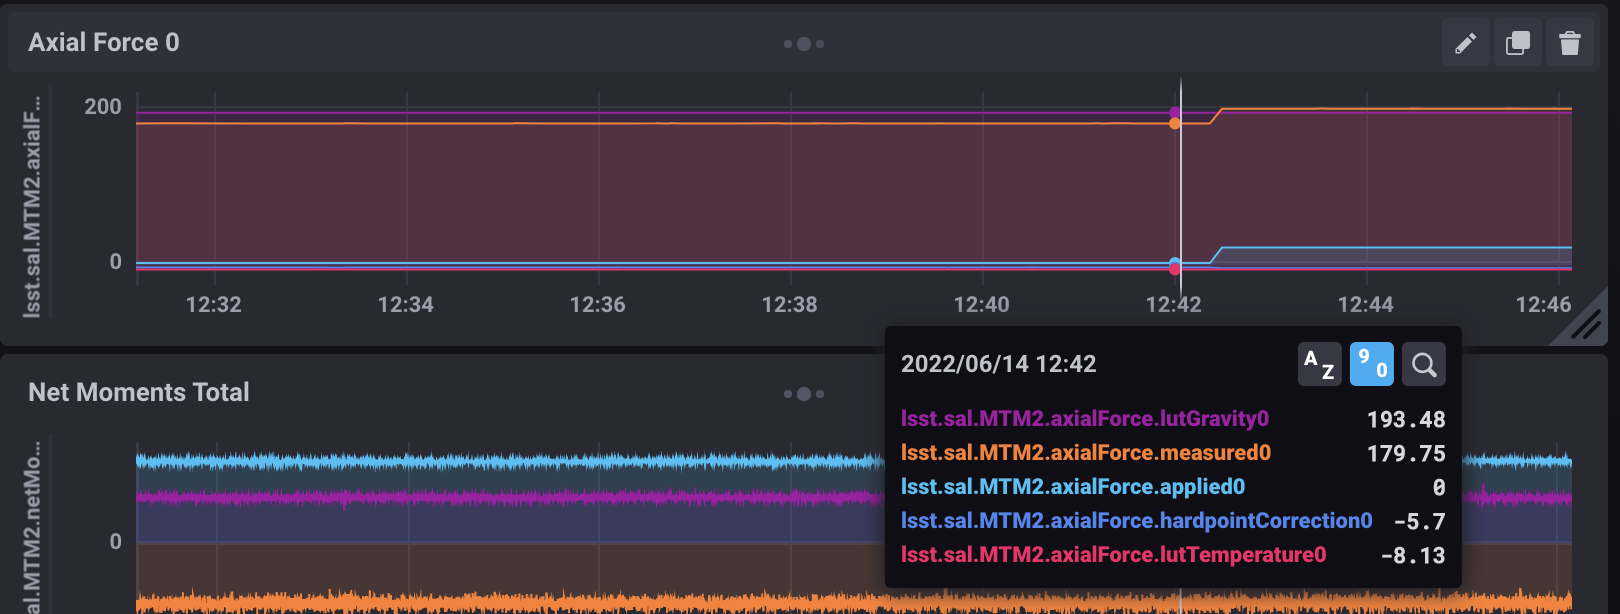
\includegraphics[width=7.41667in]{jira_imgs/2494.png}

}
\begin{tabular}{p{2cm}p{14cm}}
\toprule
Step 13 & Step Execution Status: \textbf{ Initial Pass } \\ \hline
\end{tabular}
 Description \\
{\footnotesize
Check the~\emph{MTM2\_position} topic published to the EFD.

}
\hdashrule[0.5ex]{\textwidth}{1pt}{3mm}
  Expected Result \\
{\footnotesize
The data is displayed in the EFD.

}
\hdashrule[0.5ex]{\textwidth}{1pt}{3mm}
  Actual Result \\
{\footnotesize
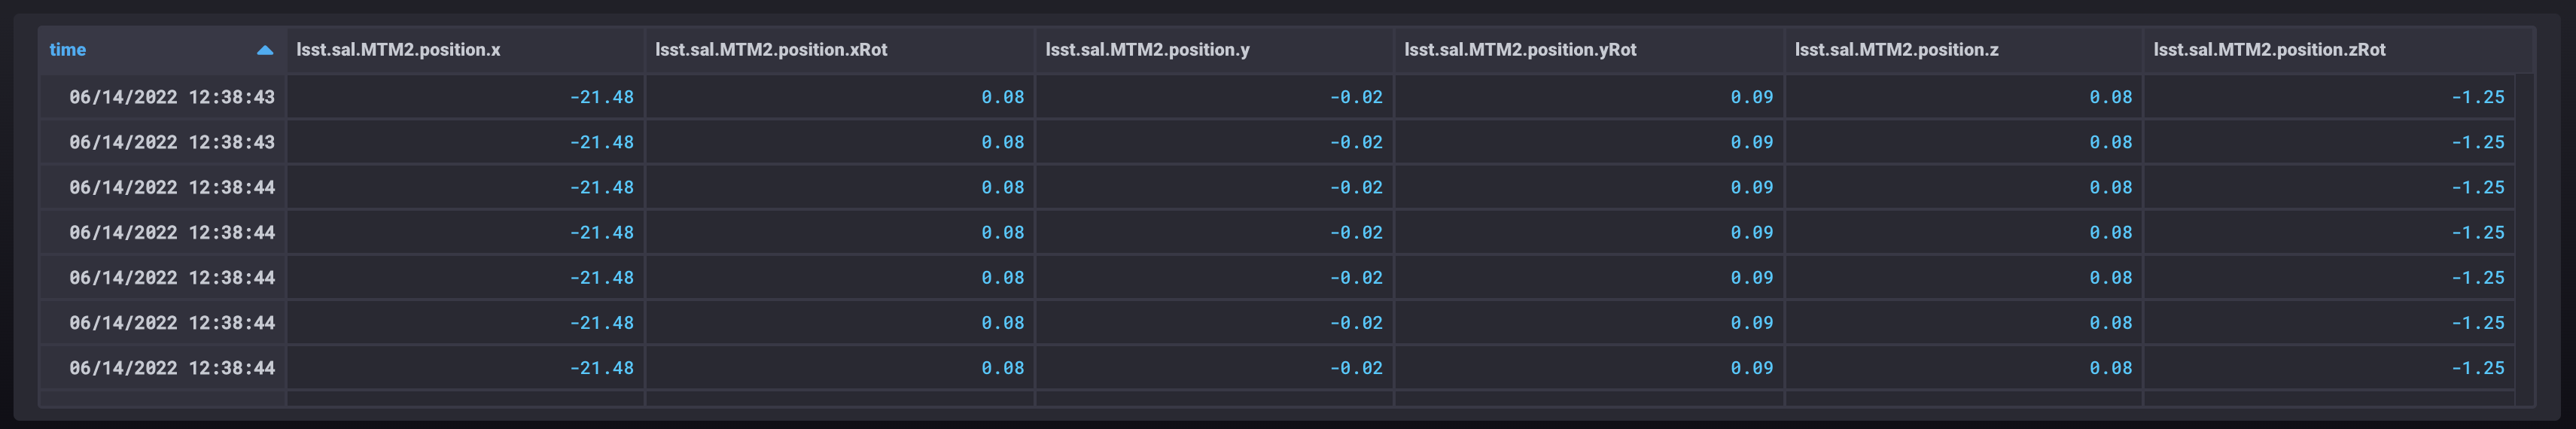
\includegraphics[width=3.12500in]{jira_imgs/2495.png}\\
The data is in the EFD. We are not checking the unit conversion.

}
\begin{tabular}{p{2cm}p{14cm}}
\toprule
Step 14 & Step Execution Status: \textbf{ Initial Pass } \\ \hline
\end{tabular}
 Description \\
{\footnotesize
Check the~\emph{MTM2\_axialForce} topic published to the EFD.

}
\hdashrule[0.5ex]{\textwidth}{1pt}{3mm}
  Expected Result \\
{\footnotesize
The data is displayed in the EFD.

}
\hdashrule[0.5ex]{\textwidth}{1pt}{3mm}
  Actual Result \\
{\footnotesize
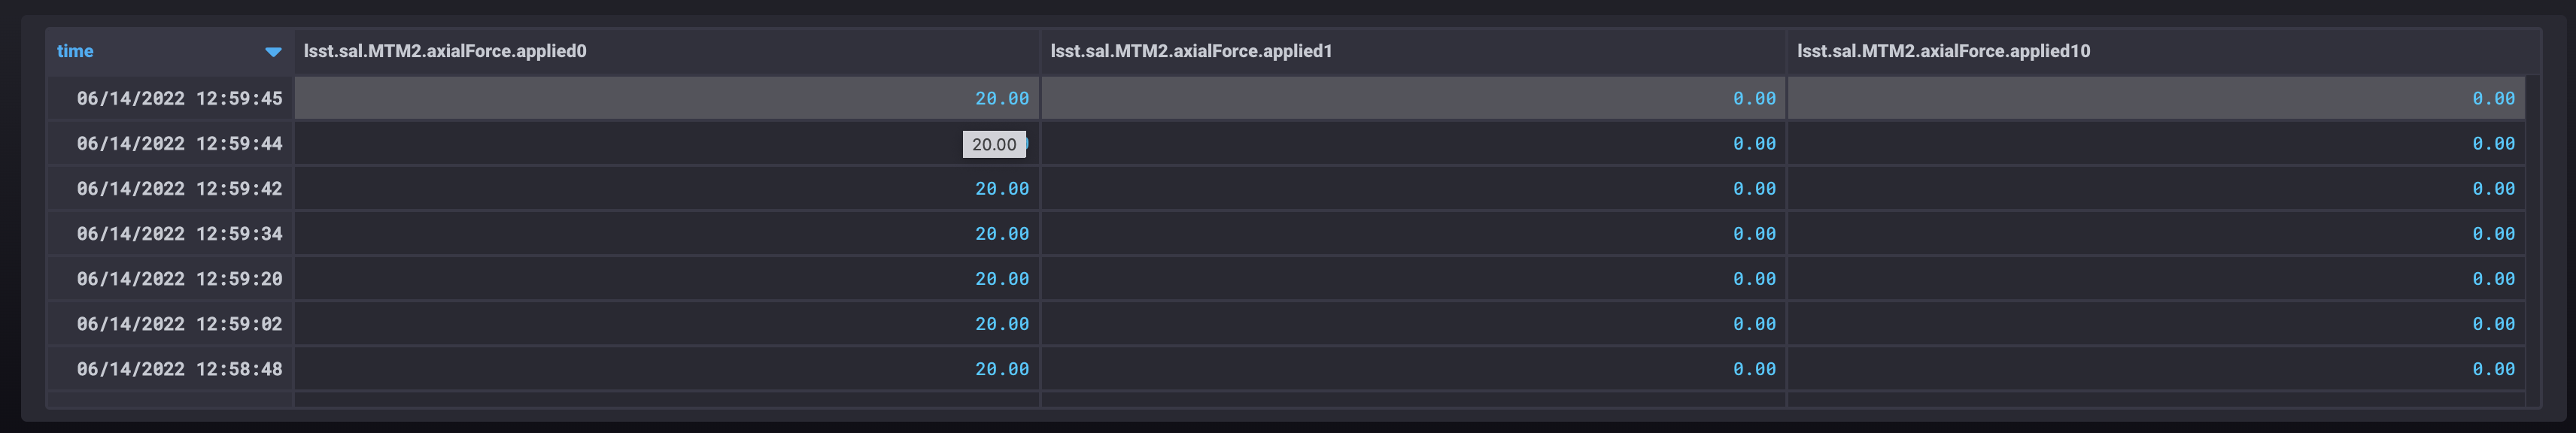
\includegraphics[width=3.12500in]{jira_imgs/2496.png}

}
\begin{tabular}{p{2cm}p{14cm}}
\toprule
Step 15 & Step Execution Status: \textbf{ Initial Pass } \\ \hline
\end{tabular}
 Description \\
{\footnotesize
Check the \emph{MTM2\_tangentForce~}topic published to the EFD.

}
\hdashrule[0.5ex]{\textwidth}{1pt}{3mm}
  Expected Result \\
{\footnotesize
The data is displayed in the EFD.

}
\hdashrule[0.5ex]{\textwidth}{1pt}{3mm}
  Actual Result \\
{\footnotesize
‚Äč‚Äč‚Äč‚ÄčAll the telemetry from LVV-T1615 can now be seen in the
following dashboard
\href{https://chronograf-summit-efd.lsst.codes:30828/sources/1/dashboards/156?refresh=Paused\&lower=now\%28\%29\%20-\%2015m}{LVV-T1615:
Integration of M2 with SAL~}\\
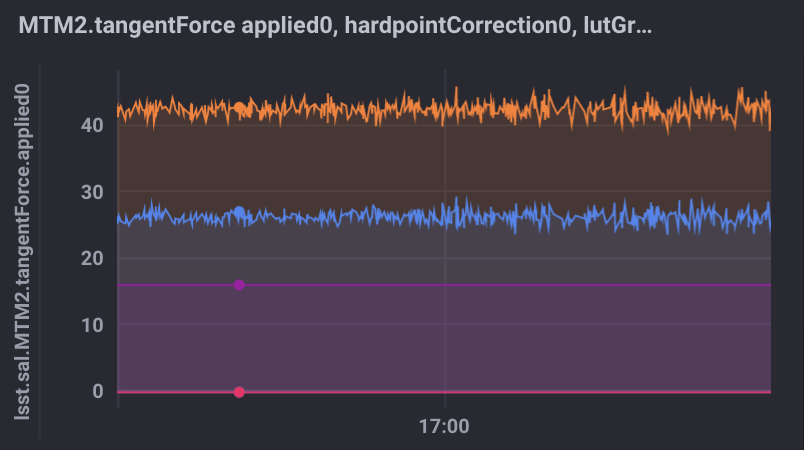
\includegraphics[width=3.12500in]{jira_imgs/2506.png}

}
\begin{tabular}{p{2cm}p{14cm}}
\toprule
Step 16 & Step Execution Status: \textbf{ Initial Pass } \\ \hline
\end{tabular}
 Description \\
{\footnotesize
Check the \emph{MTM2\_forceBalance~}topic published to the EFD.

}
\hdashrule[0.5ex]{\textwidth}{1pt}{3mm}
  Expected Result \\
{\footnotesize
The data is displayed in the EFD.

}
\hdashrule[0.5ex]{\textwidth}{1pt}{3mm}
  Actual Result \\
{\footnotesize
The telemetry evaluated in LVV-T1615 can now be seen in the following
live dashboard
\href{https://chronograf-summit-efd.lsst.codes:30828/sources/1/dashboards/156?refresh=Paused\&lower=now\%28\%29\%20-\%2015m}{LVV-T1615:
Integration of M2 with SAL~}\\
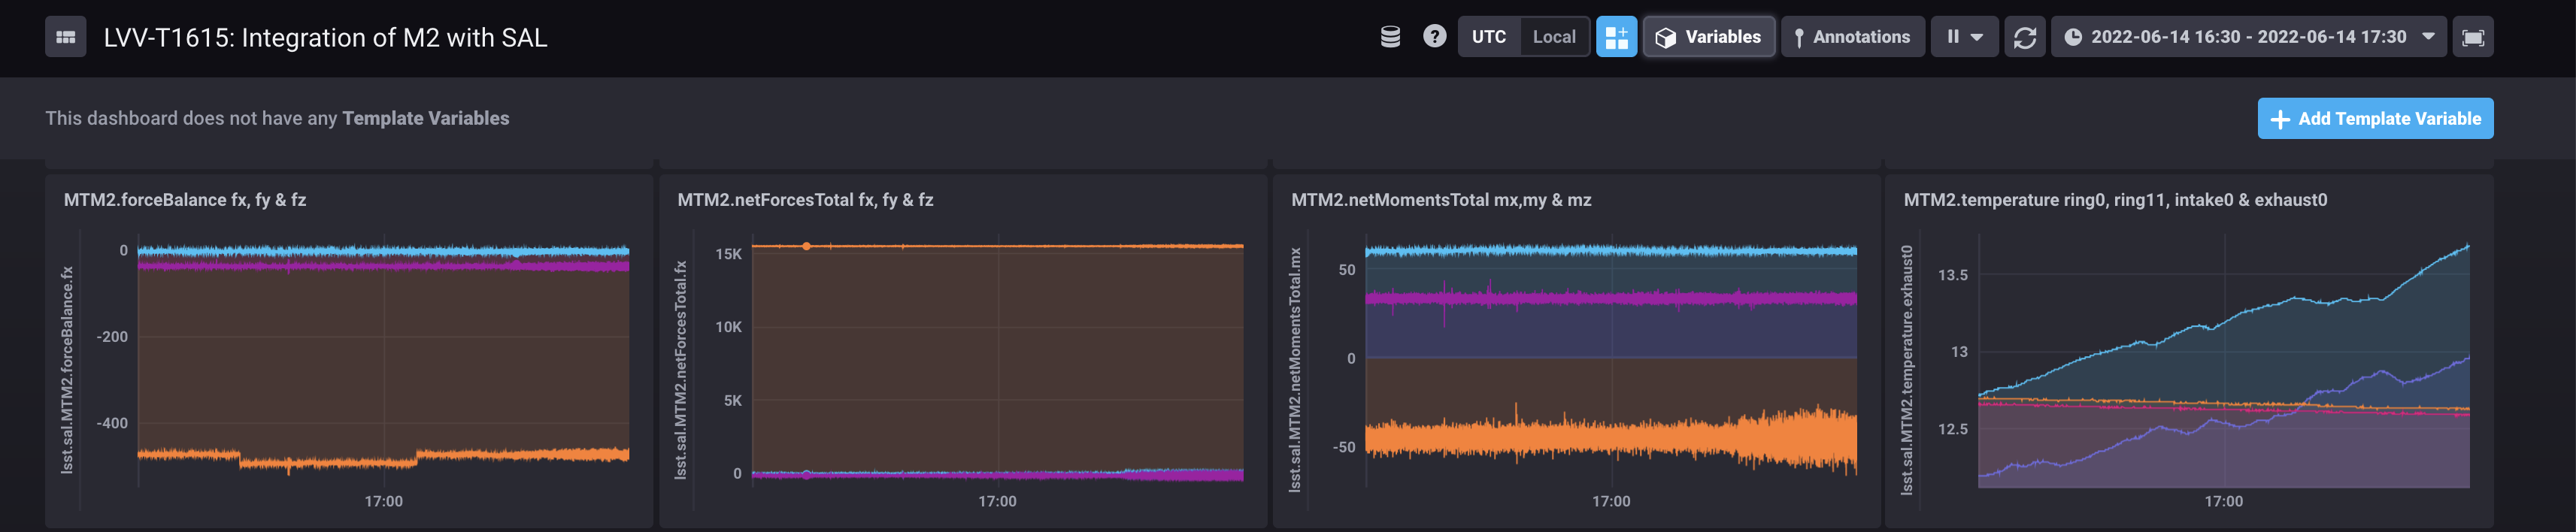
\includegraphics[width=7.82292in]{jira_imgs/2519.png}

}
\begin{tabular}{p{2cm}p{14cm}}
\toprule
Step 17 & Step Execution Status: \textbf{ Initial Pass } \\ \hline
\end{tabular}
 Description \\
{\footnotesize
Check the \emph{MTM2\_netForcesTotal} topic published to the EFD.

}
\hdashrule[0.5ex]{\textwidth}{1pt}{3mm}
  Expected Result \\
{\footnotesize
The data is displayed in the EFD.

}
\hdashrule[0.5ex]{\textwidth}{1pt}{3mm}
  Actual Result \\
{\footnotesize
The telemetry evaluated in LVV-T1615 can now be seen in the following
live dashboard
\href{https://chronograf-summit-efd.lsst.codes:30828/sources/1/dashboards/156?refresh=Paused\&lower=now\%28\%29\%20-\%2015m}{LVV-T1615:
Integration of M2 with SAL}. From 16:30 to 17:30 UT\\
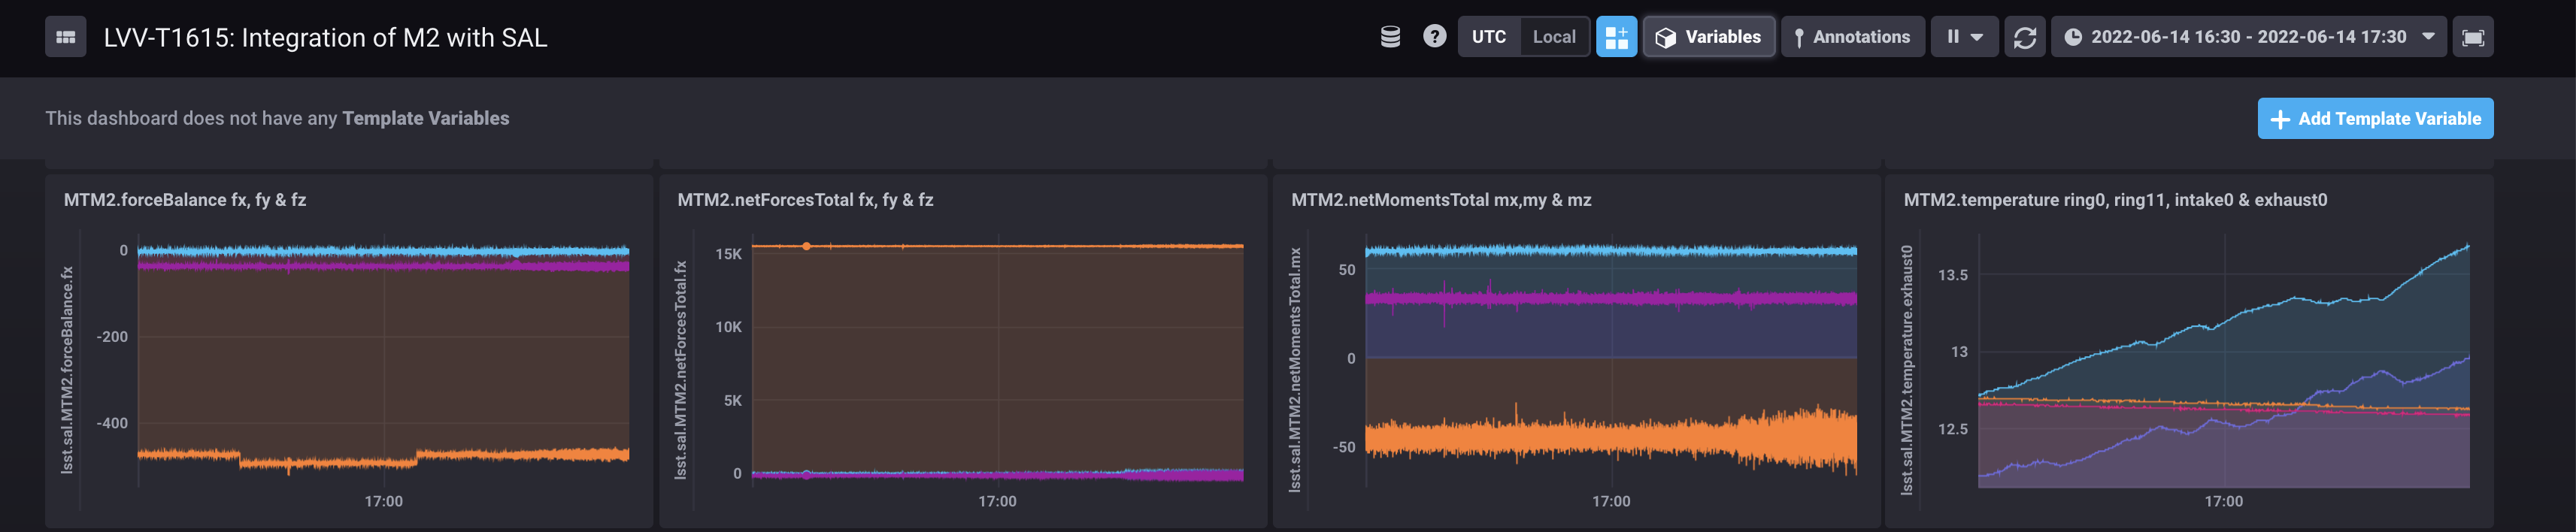
\includegraphics[width=7.77083in]{jira_imgs/2520.png}

}
\begin{tabular}{p{2cm}p{14cm}}
\toprule
Step 18 & Step Execution Status: \textbf{ Initial Pass } \\ \hline
\end{tabular}
 Description \\
{\footnotesize
Check the \emph{MTM2\_netMomentsTotal} topic published to the EFD.

}
\hdashrule[0.5ex]{\textwidth}{1pt}{3mm}
  Expected Result \\
{\footnotesize
The data is displayed in the EFD.

}
\hdashrule[0.5ex]{\textwidth}{1pt}{3mm}
  Actual Result \\
{\footnotesize
The telemetry evaluated in LVV-T1615 can now be seen in the following
live dashboard
\href{https://chronograf-summit-efd.lsst.codes:30828/sources/1/dashboards/156?refresh=Paused\&lower=now\%28\%29\%20-\%2015m}{LVV-T1615:
Integration of M2 with SAL}. From 16:30 to 17:30 UT\\
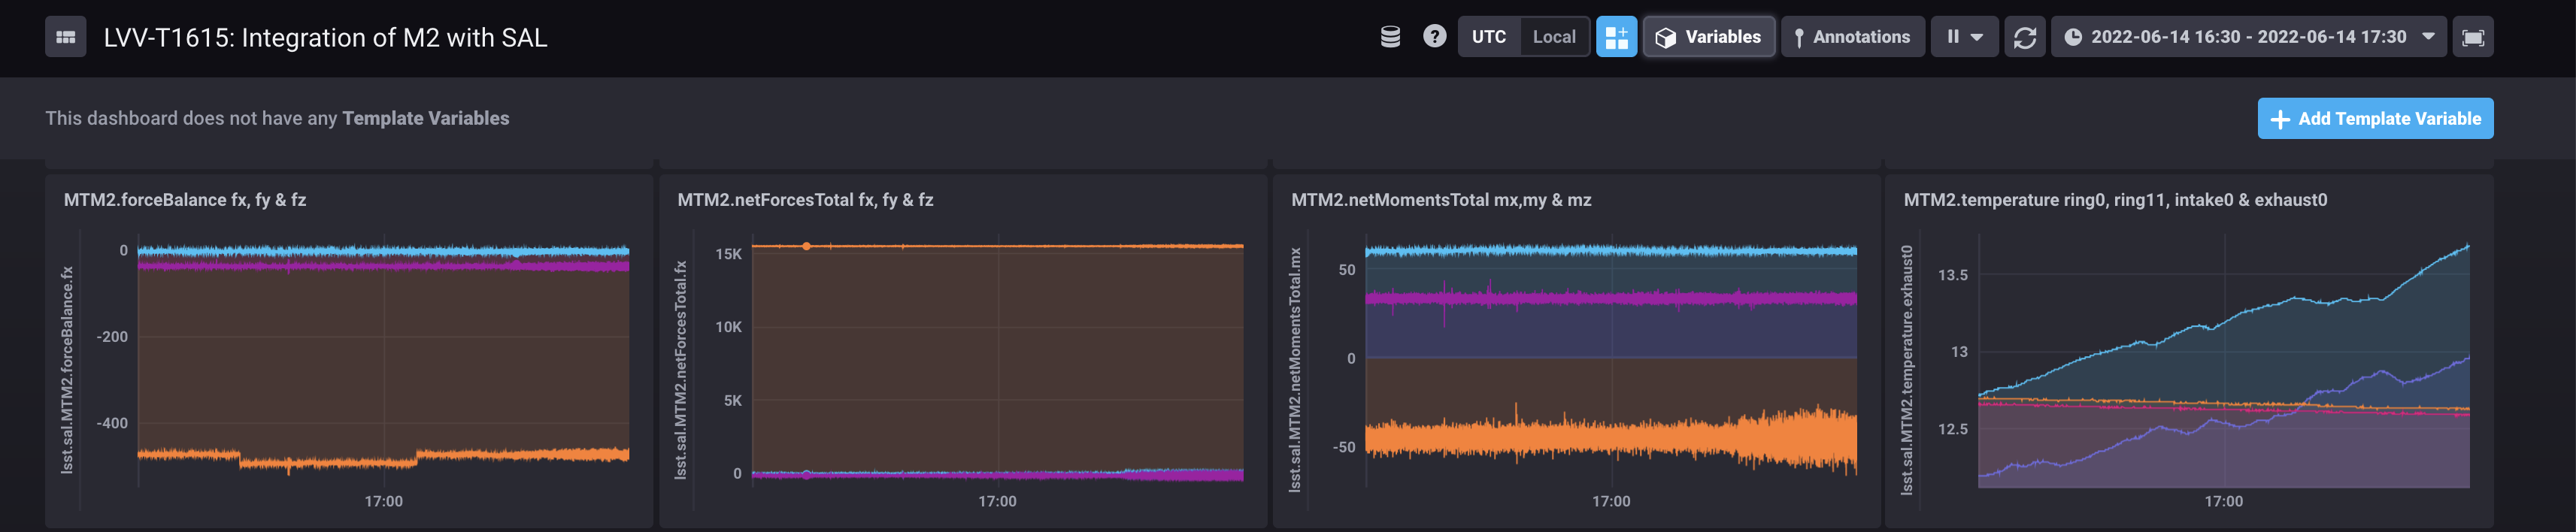
\includegraphics[width=7.86458in]{jira_imgs/2520.png}\\

}
\begin{tabular}{p{2cm}p{14cm}}
\toprule
Step 19 & Step Execution Status: \textbf{ Initial Pass } \\ \hline
\end{tabular}
 Description \\
{\footnotesize
Check the \emph{MTM2\_temperature} topic published to the EFD.

}
\hdashrule[0.5ex]{\textwidth}{1pt}{3mm}
  Expected Result \\
{\footnotesize
The data is displayed in the EFD.

}
\hdashrule[0.5ex]{\textwidth}{1pt}{3mm}
  Actual Result \\
{\footnotesize
The telemetry evaluated in LVV-T1615 can now be seen in the following
live dashboard
\href{https://chronograf-summit-efd.lsst.codes:30828/sources/1/dashboards/156?refresh=Paused\&lower=now\%28\%29\%20-\%2015m}{LVV-T1615:
Integration of M2 with SAL}. From 16:30 to 17:30 UT\\
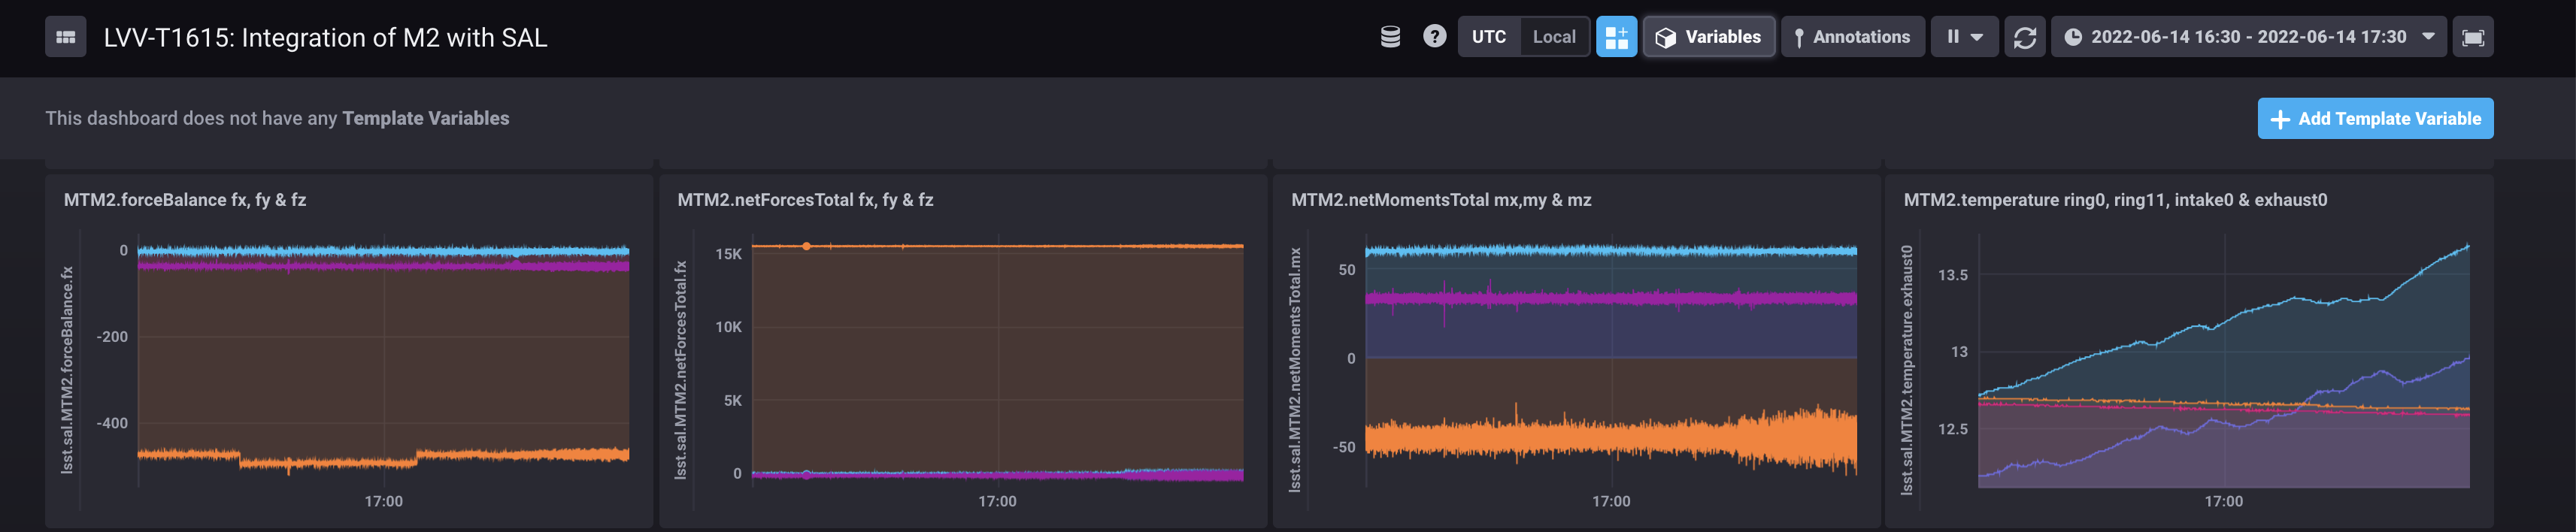
\includegraphics[width=7.76042in]{jira_imgs/2520.png}\\

}
\begin{tabular}{p{2cm}p{14cm}}
\toprule
Step 20 & Step Execution Status: \textbf{ Initial Pass } \\ \hline
\end{tabular}
 Description \\
{\footnotesize
Check the \emph{MTM2\_zenithAngle} topic published to the EFD.

}
\hdashrule[0.5ex]{\textwidth}{1pt}{3mm}
  Expected Result \\
{\footnotesize
The data is consistent with what is on the EUI display and the EFD and
the units are degrees.

}
\hdashrule[0.5ex]{\textwidth}{1pt}{3mm}
  Actual Result \\
{\footnotesize
The telemetry evaluated in this step can be seen in the Chronograph
dashboard
\href{https://chronograf-summit-efd.lsst.codes:30828/sources/1/dashboards/156?refresh=Paused\&lower=now\%28\%29\%20-\%2015m}{LVV-T1615:
Integration of M2 with SAL}.~\\
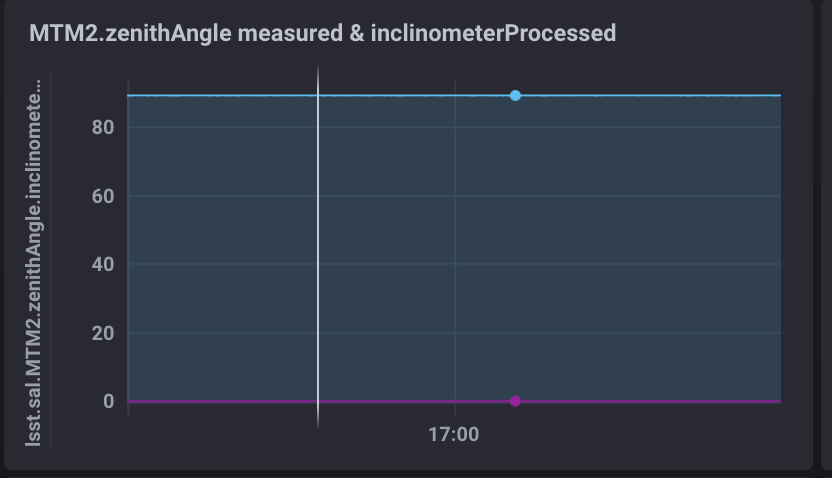
\includegraphics[width=3.12500in]{jira_imgs/2513.png}

}
\begin{tabular}{p{2cm}p{14cm}}
\toprule
Step 21 & Step Execution Status: \textbf{ Initial Pass } \\ \hline
\end{tabular}
 Description \\
{\footnotesize
Check the \emph{MTM2\_axialActutatorSteps} topic published to the EFD.

}
\hdashrule[0.5ex]{\textwidth}{1pt}{3mm}
  Expected Result \\
{\footnotesize
The data is displayed in the EFD.

}
\hdashrule[0.5ex]{\textwidth}{1pt}{3mm}
  Actual Result \\
{\footnotesize
The telemetry evaluated in this step can be seen in the Chronograph
dashboard
\href{https://chronograf-summit-efd.lsst.codes:30828/sources/1/dashboards/156?refresh=Paused\&lower=now\%28\%29\%20-\%2015m}{LVV-T1615:
Integration of M2 with SAL}.\\
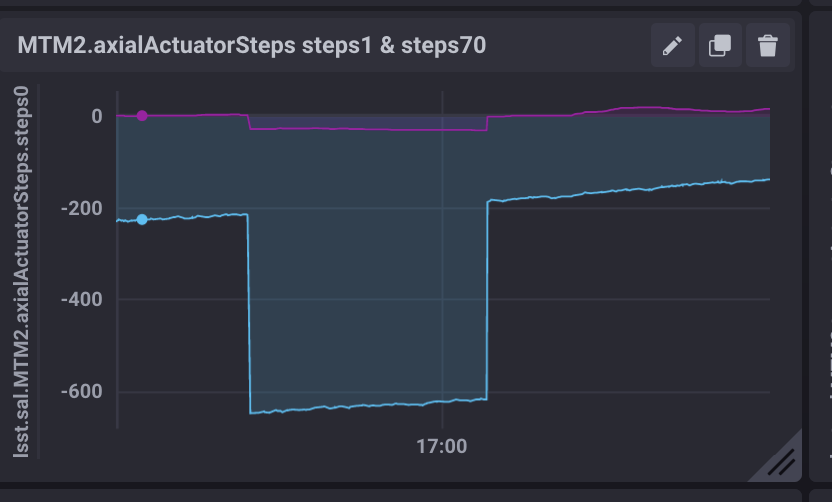
\includegraphics[width=3.12500in]{jira_imgs/2514.png}

}
\begin{tabular}{p{2cm}p{14cm}}
\toprule
Step 22 & Step Execution Status: \textbf{ Initial Pass } \\ \hline
\end{tabular}
 Description \\
{\footnotesize
Check the \emph{MTM2\_tangentActuatorSteps} topic published to the EFD

}
\hdashrule[0.5ex]{\textwidth}{1pt}{3mm}
  Expected Result \\
{\footnotesize
The data is displayed in the EFD.

}
\hdashrule[0.5ex]{\textwidth}{1pt}{3mm}
  Actual Result \\
{\footnotesize
The telemetry evaluated in this step can be seen in the Chronograph
dashboard
\href{https://chronograf-summit-efd.lsst.codes:30828/sources/1/dashboards/156?refresh=Paused\&lower=now\%28\%29\%20-\%2015m}{LVV-T1615:
Integration of M2 with SAL}.\\
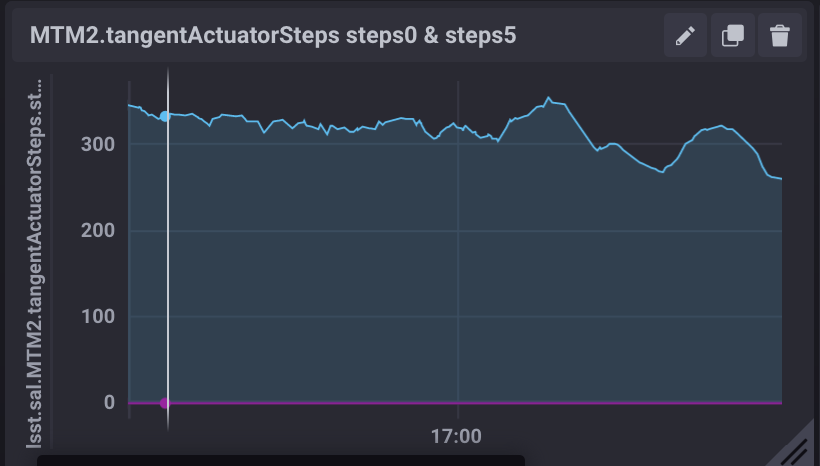
\includegraphics[width=3.12500in]{jira_imgs/2515.png}

}
\begin{tabular}{p{2cm}p{14cm}}
\toprule
Step 23 & Step Execution Status: \textbf{ Initial Pass } \\ \hline
\end{tabular}
 Description \\
{\footnotesize
Check the \emph{MTM2\_axialEncoderPositions} topic published to the EFD.

}
\hdashrule[0.5ex]{\textwidth}{1pt}{3mm}
  Expected Result \\
{\footnotesize
The data is displayed in the EFD.

}
\hdashrule[0.5ex]{\textwidth}{1pt}{3mm}
  Actual Result \\
{\footnotesize
The telemetry evaluated in this step can be seen in the Chronograph
dashboard
\href{https://chronograf-summit-efd.lsst.codes:30828/sources/1/dashboards/156?refresh=Paused\&lower=now\%28\%29\%20-\%2015m}{LVV-T1615:
Integration of M2 with SAL}.\\
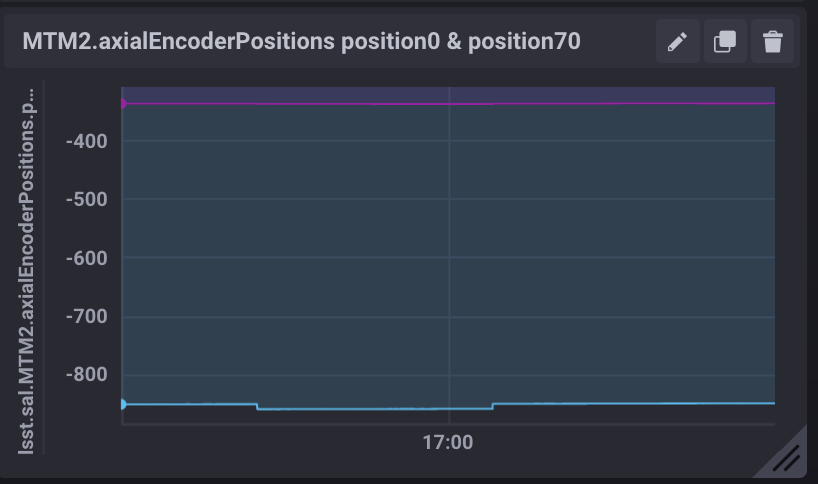
\includegraphics[width=3.12500in]{jira_imgs/2516.png}

}
\begin{tabular}{p{2cm}p{14cm}}
\toprule
Step 24 & Step Execution Status: \textbf{ Initial Pass } \\ \hline
\end{tabular}
 Description \\
{\footnotesize
Check the \emph{MTM2\_tangentEncoderPositions~}topic published to the
EFD.

}
\hdashrule[0.5ex]{\textwidth}{1pt}{3mm}
  Expected Result \\
{\footnotesize
The data is displayed in the EFD.

}
\hdashrule[0.5ex]{\textwidth}{1pt}{3mm}
  Actual Result \\
{\footnotesize
The telemetry evaluated in this step can be seen in the Chronograph
dashboard
\href{https://chronograf-summit-efd.lsst.codes:30828/sources/1/dashboards/156?refresh=Paused\&lower=now\%28\%29\%20-\%2015m}{LVV-T1615:
Integration of M2 with SAL}.\\
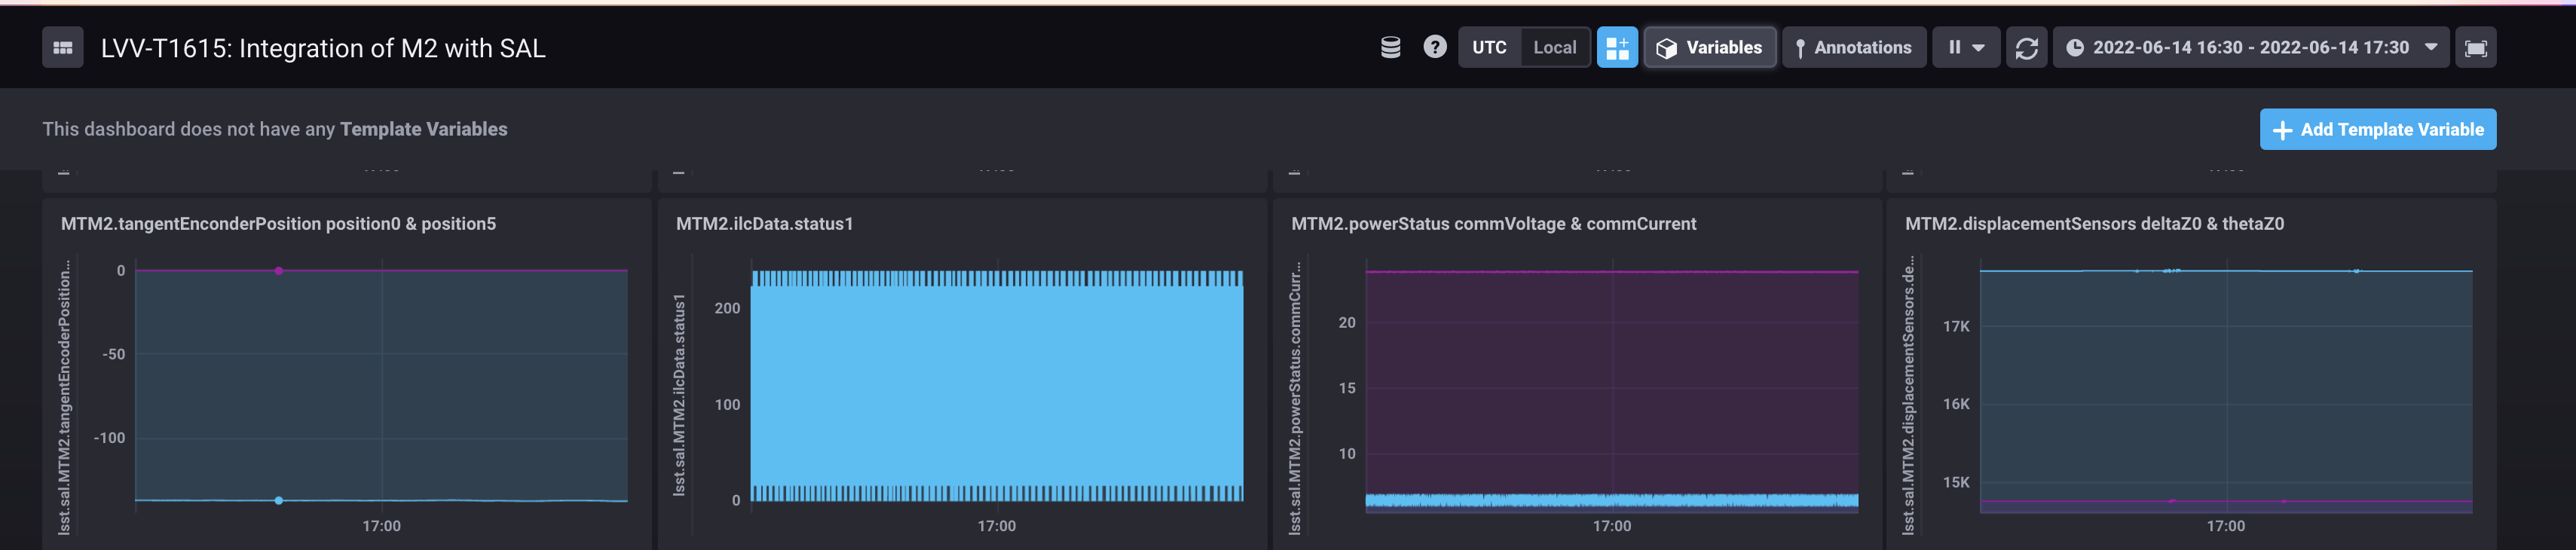
\includegraphics[width=8.12500in]{jira_imgs/2517.png}

}
\begin{tabular}{p{2cm}p{14cm}}
\toprule
Step 25 & Step Execution Status: \textbf{ Initial Pass } \\ \hline
\end{tabular}
 Description \\
{\footnotesize
Check the {\emph{MTM2\_ilcData}} topic published to the EFD.

}
\hdashrule[0.5ex]{\textwidth}{1pt}{3mm}
  Expected Result \\
{\footnotesize
The data is displayed in the EFD.

}
\hdashrule[0.5ex]{\textwidth}{1pt}{3mm}
  Actual Result \\
{\footnotesize
The telemetry evaluated in this step can be seen in the Chronograph
dashboard
\href{https://chronograf-summit-efd.lsst.codes:30828/sources/1/dashboards/156?refresh=Paused\&lower=now\%28\%29\%20-\%2015m}{LVV-T1615:
Integration of M2 with SAL}.\\
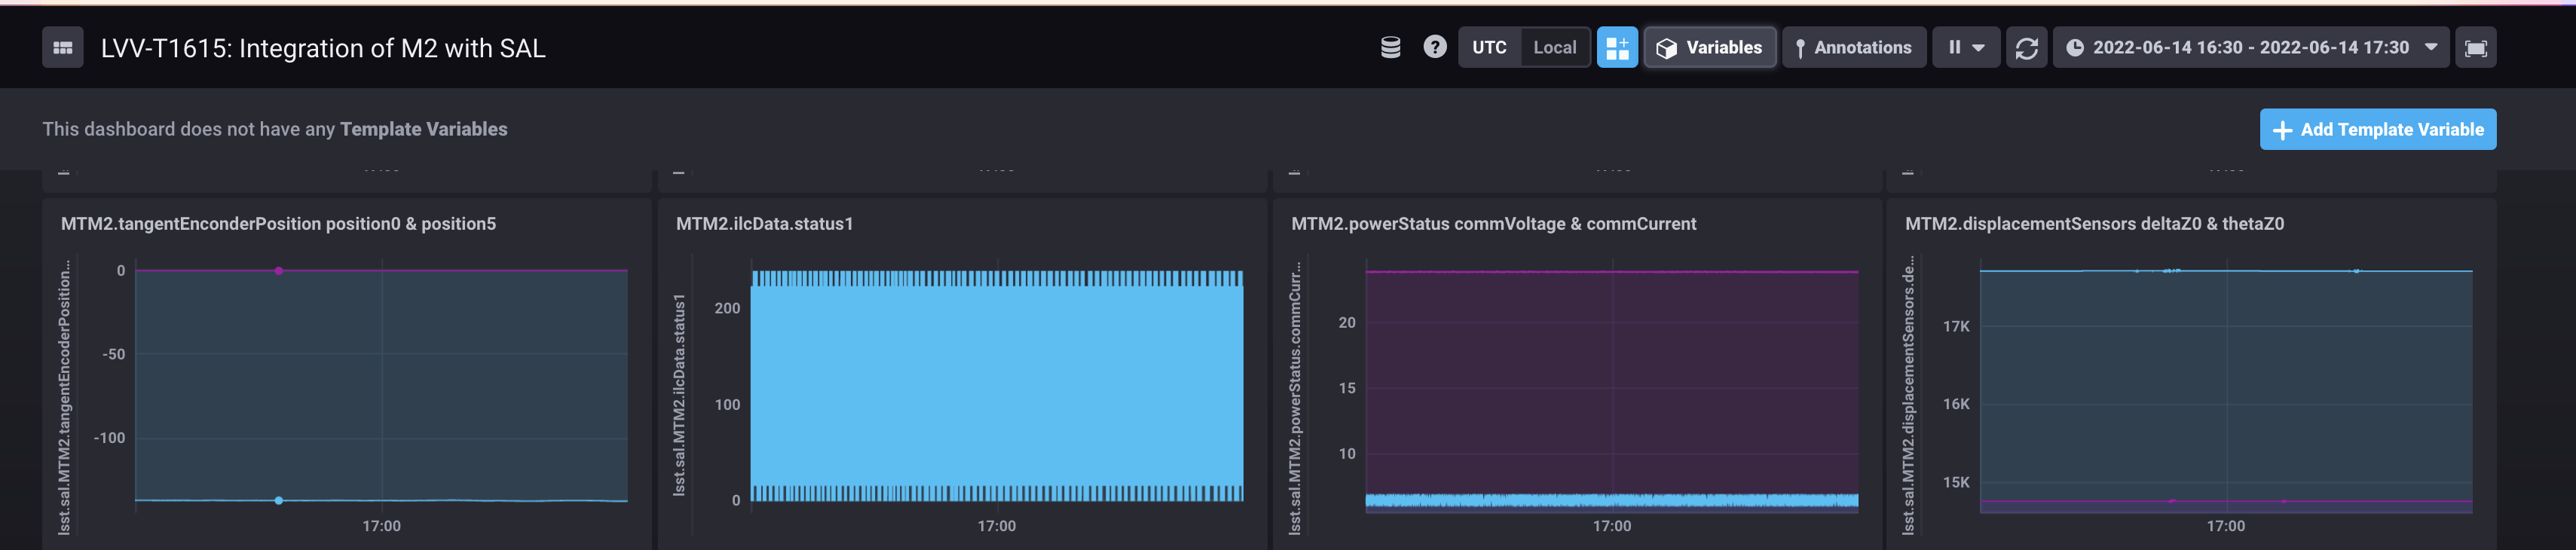
\includegraphics[width=8.05208in]{jira_imgs/2517.png}\\

}
\begin{tabular}{p{2cm}p{14cm}}
\toprule
Step 26 & Step Execution Status: \textbf{ Initial Pass } \\ \hline
\end{tabular}
 Description \\
{\footnotesize
Check the \emph{MTM2\_powerStatus} topic published to the EFD.

}
\hdashrule[0.5ex]{\textwidth}{1pt}{3mm}
  Expected Result \\
{\footnotesize
The data is displayed in the EFD.

}
\hdashrule[0.5ex]{\textwidth}{1pt}{3mm}
  Actual Result \\
{\footnotesize
The telemetry evaluated in this step can be seen in the Chronograph
dashboard
\href{https://chronograf-summit-efd.lsst.codes:30828/sources/1/dashboards/156?refresh=Paused\&lower=now\%28\%29\%20-\%2015m}{LVV-T1615:
Integration of M2 with SAL}.\\
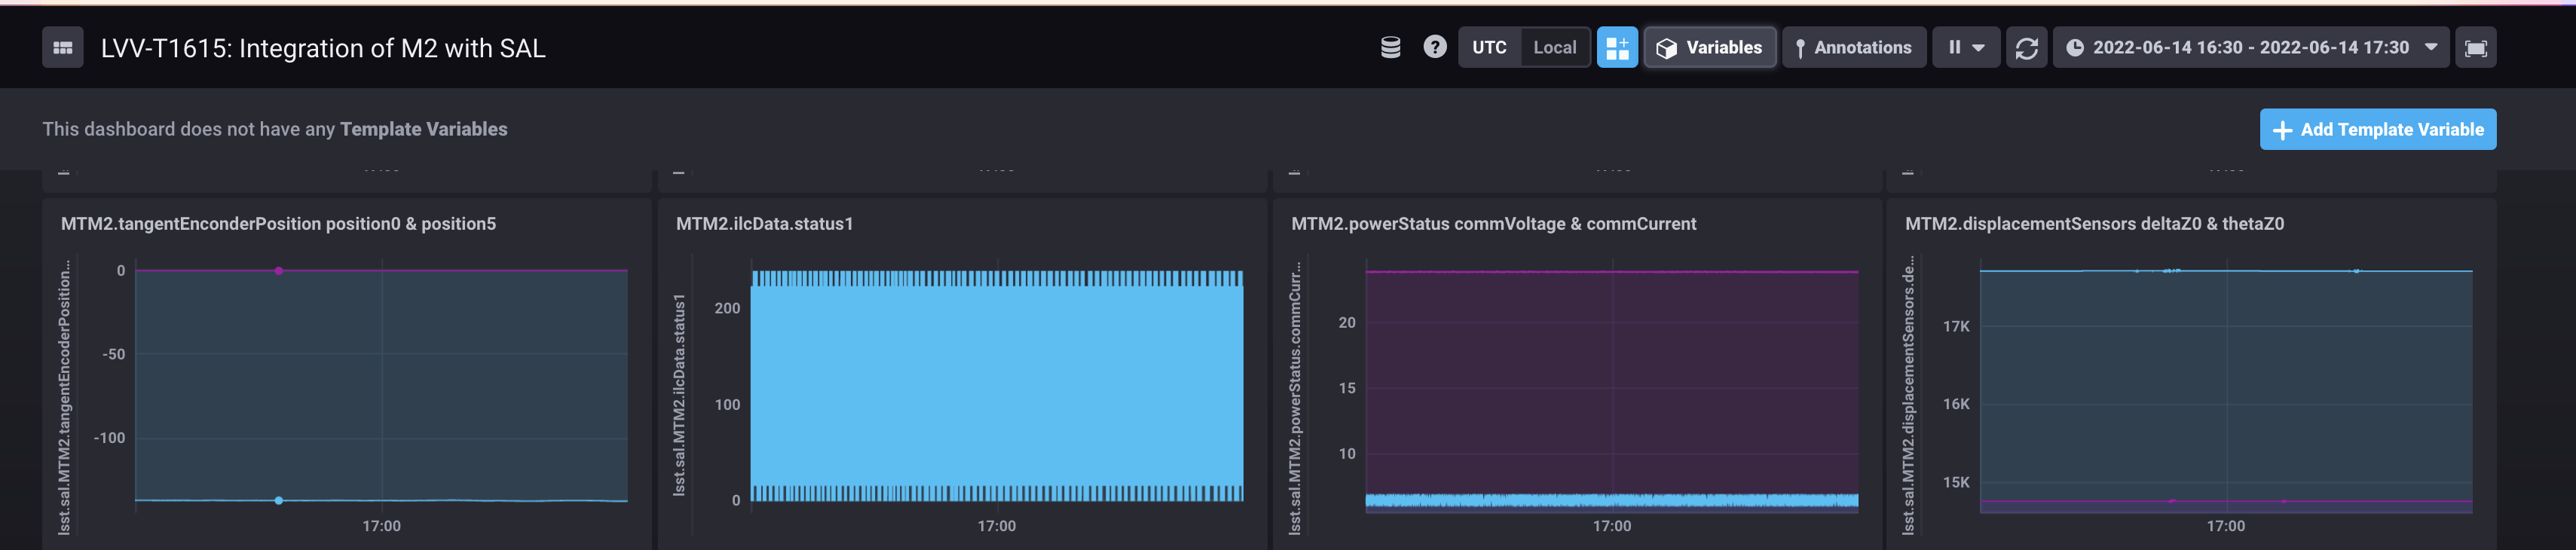
\includegraphics[width=8.07292in]{jira_imgs/2517.png}\\

}
\begin{tabular}{p{2cm}p{14cm}}
\toprule
Step 27 & Step Execution Status: \textbf{ Initial Pass } \\ \hline
\end{tabular}
 Description \\
{\footnotesize
Check the {\emph{MTM2\_displacementSensors}} topic published to the EFD.

}
\hdashrule[0.5ex]{\textwidth}{1pt}{3mm}
  Expected Result \\
{\footnotesize
The data is displayed in the EFD.

}
\hdashrule[0.5ex]{\textwidth}{1pt}{3mm}
  Actual Result \\
{\footnotesize
The telemetry evaluated in this step can be seen in the Chronograph
dashboard
\href{https://chronograf-summit-efd.lsst.codes:30828/sources/1/dashboards/156?refresh=Paused\&lower=now\%28\%29\%20-\%2015m}{LVV-T1615:
Integration of M2 with SAL}.\\
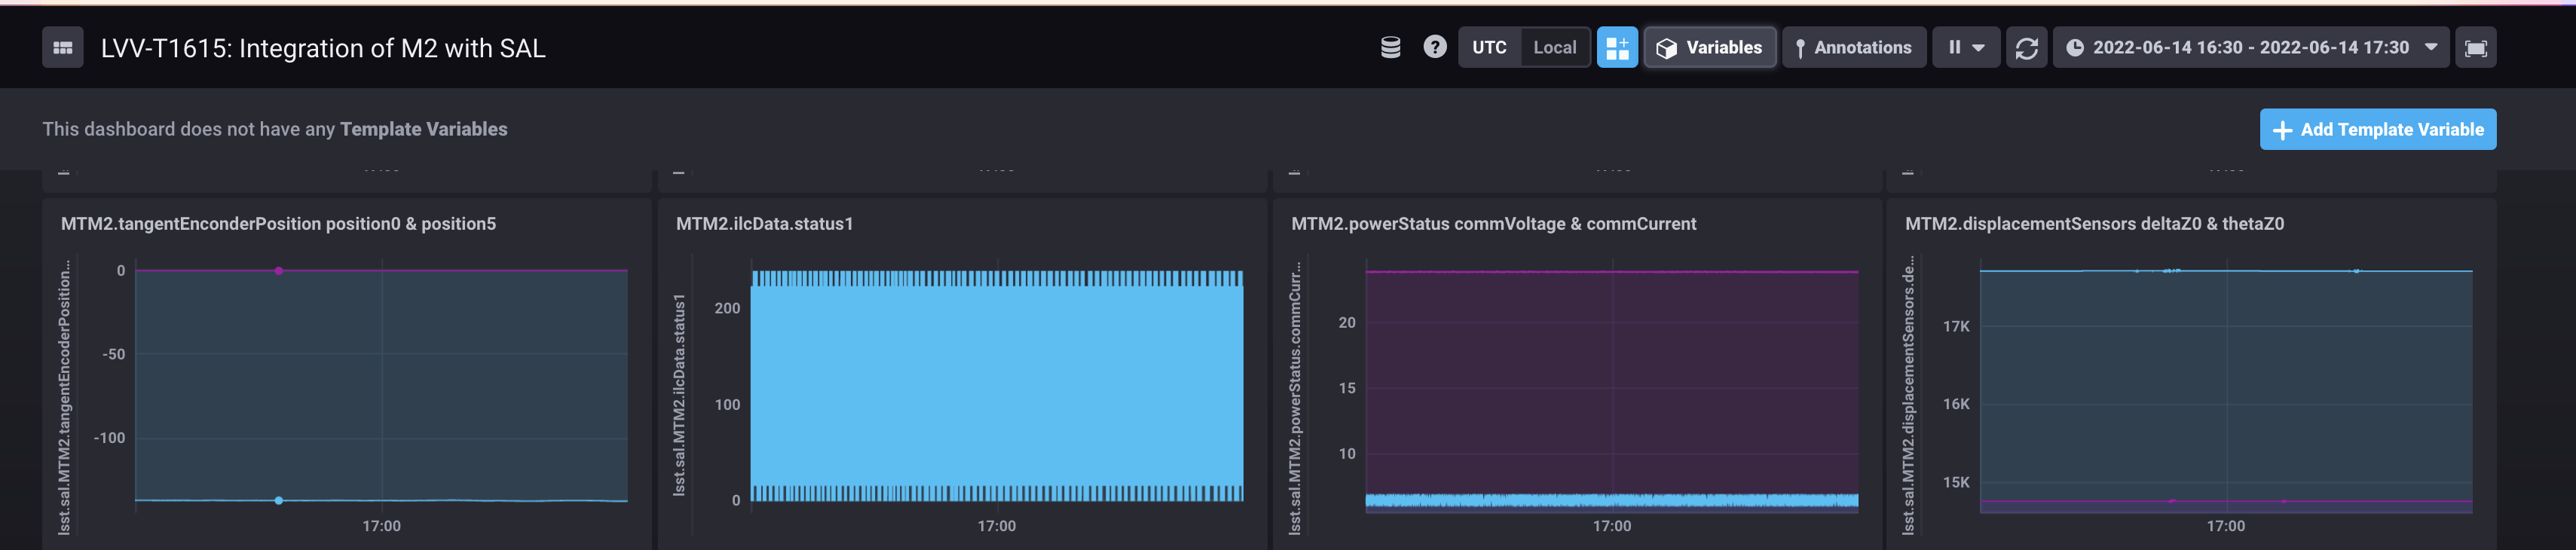
\includegraphics[width=8.27083in]{jira_imgs/2517.png}\\

}
\begin{tabular}{p{2cm}p{14cm}}
\toprule
Step 28 & Step Execution Status: \textbf{ Initial Pass } \\ \hline
\end{tabular}
 Description \\
{\footnotesize
Check the \emph{MTM2\_positionIMS} topic published to the EFD.

}
\hdashrule[0.5ex]{\textwidth}{1pt}{3mm}
  Expected Result \\
{\footnotesize
The data is displayed in the EFD.

}
\hdashrule[0.5ex]{\textwidth}{1pt}{3mm}
  Actual Result \\
{\footnotesize
The telemetry evaluated in this step can be seen in the Chronograph
dashboard
\href{https://chronograf-summit-efd.lsst.codes:30828/sources/1/dashboards/156?refresh=Paused\&lower=now\%28\%29\%20-\%2015m}{LVV-T1615:
Integration of M2 with SAL}.\\
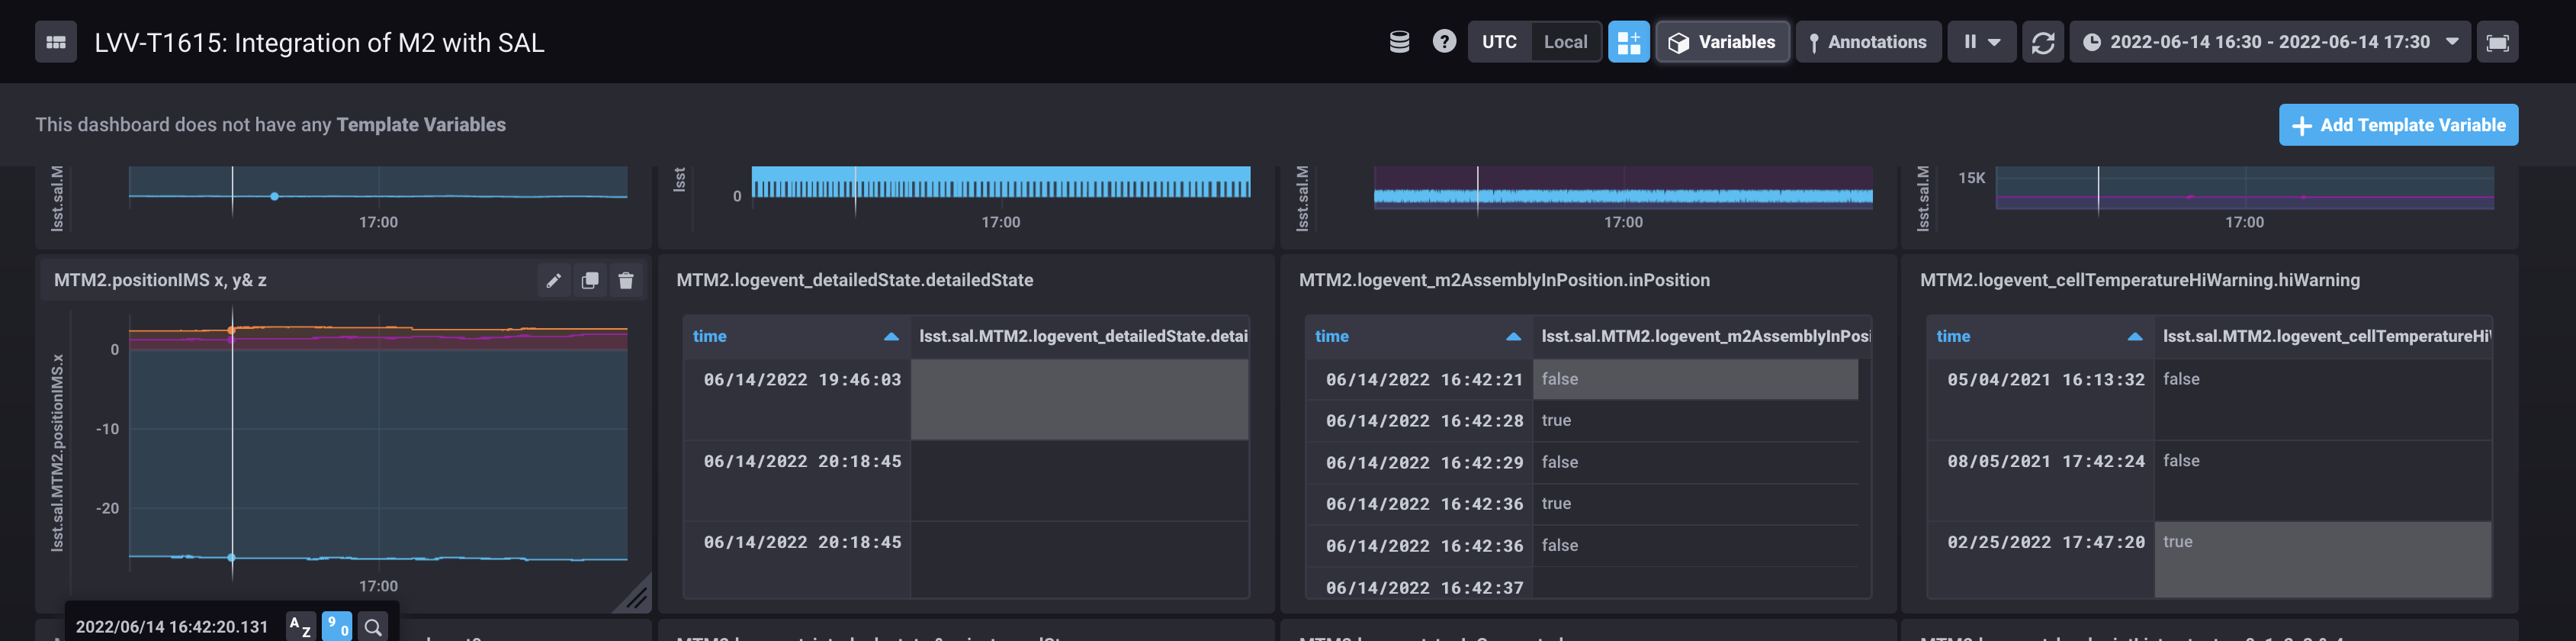
\includegraphics[width=3.12500in]{jira_imgs/2518.png}

}
\begin{tabular}{p{2cm}p{14cm}}
\toprule
Step 29 & Step Execution Status: \textbf{ Not Executed } \\ \hline
\end{tabular}
 Description \\
{\footnotesize
Check that the GUI has been updated to match the categorization of the
forces in the SAL telemetry

}
\hdashrule[0.5ex]{\textwidth}{1pt}{3mm}
  Expected Result \\
{\footnotesize
The GUI should include the total forces, measured forces, LUT\_gravity
forces, LUT\_thermal forces, user\_applied forces (including AOS
forces), and balance forces

}
\hdashrule[0.5ex]{\textwidth}{1pt}{3mm}
  Actual Result \\
{\footnotesize

}
\begin{tabular}{p{2cm}p{14cm}}
\toprule
Step 30 & Step Execution Status: \textbf{ Fail } \\ \hline
\end{tabular}
 Description \\
{\footnotesize
\textbf{M2 Assembly detailed state}\\[2\baselineskip]Verify the
\emph{MTM2\_logevent\_detailedState} event is published to the EFD.

}
\hdashrule[0.5ex]{\textwidth}{1pt}{3mm}
  Expected Result \\
{\footnotesize
The M2 Assembly publishes the values of the detailed state.

}
\hdashrule[0.5ex]{\textwidth}{1pt}{3mm}
  Actual Result \\
{\footnotesize
This event does not show up in the Chronograph, nor it was published in
the EFD during the test window:\\
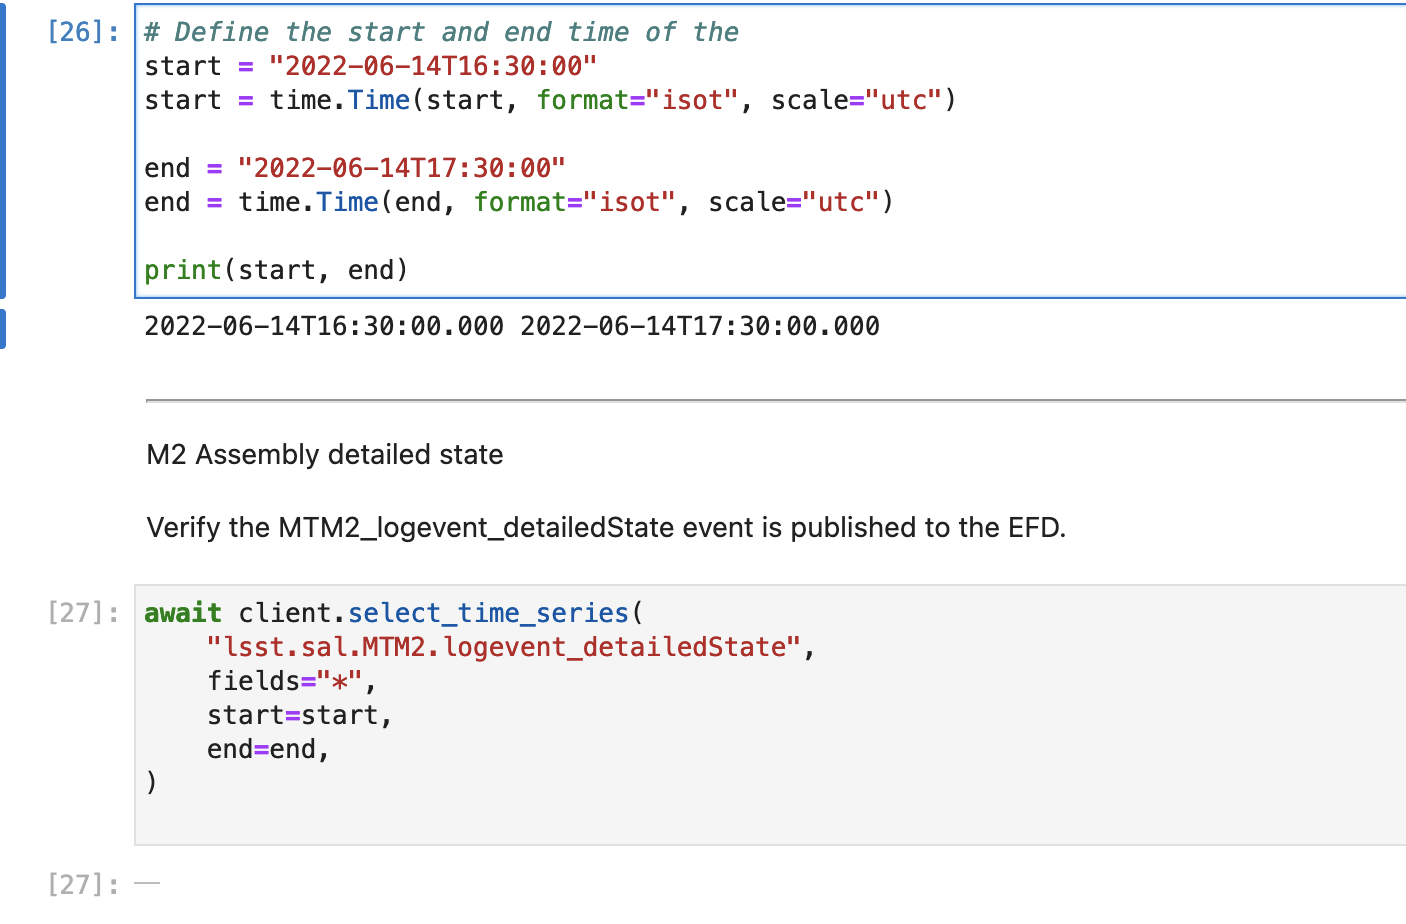
\includegraphics[width=3.12500in]{jira_imgs/2525.png}

}
\begin{tabular}{p{2cm}p{14cm}}
\toprule
Step 31 & Step Execution Status: \textbf{ Fail } \\ \hline
\end{tabular}
 Description \\
{\footnotesize
\textbf{M2 Assembly Controller State}\\[2\baselineskip]Verify the
\emph{MTM2\_logevent\_controllerState} event is published to the EFD.

}
\hdashrule[0.5ex]{\textwidth}{1pt}{3mm}
  Expected Result \\
{\footnotesize
The M2 Assembly publishes the values of the controller state~

}
\hdashrule[0.5ex]{\textwidth}{1pt}{3mm}
  Actual Result \\
{\footnotesize
This event does not show up in the Chronograph, nor it was published in
the EFD during the test window:\\
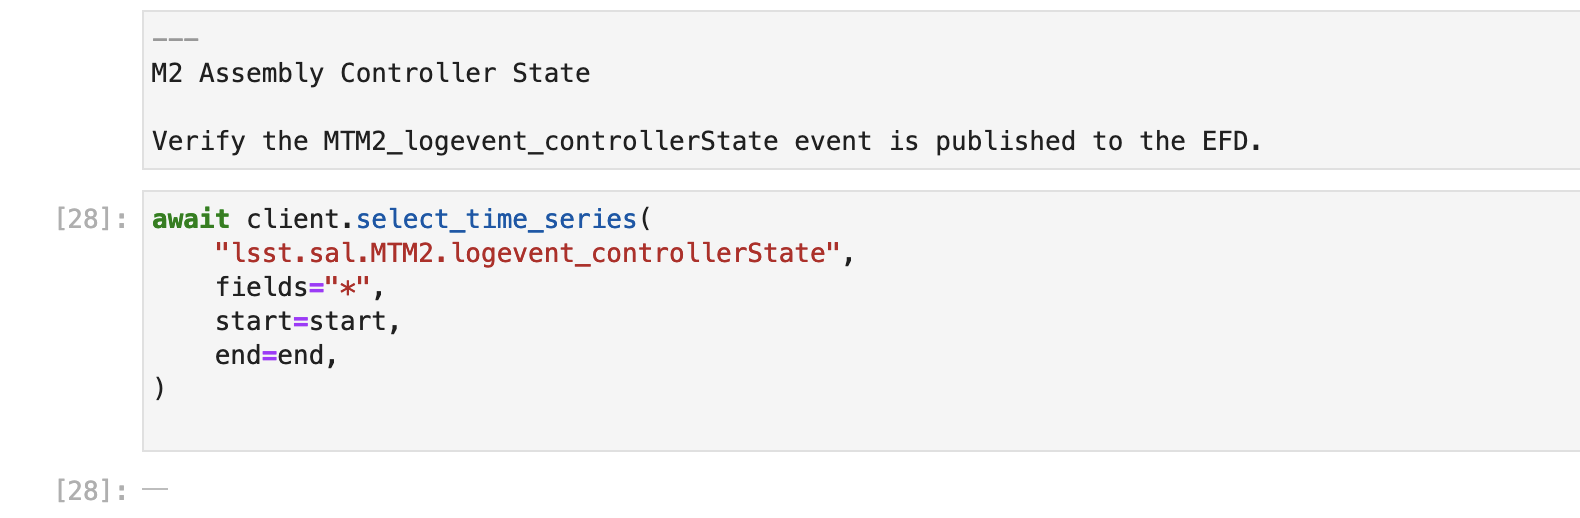
\includegraphics[width=3.12500in]{jira_imgs/2526.png}

}
\begin{tabular}{p{2cm}p{14cm}}
\toprule
Step 32 & Step Execution Status: \textbf{ Initial Pass } \\ \hline
\end{tabular}
 Description \\
{\footnotesize
\textbf{M2 Assembly inPosition}\\[2\baselineskip]Verify that
\emph{MTM2\_logevent\_m2AssemblyInPosition} event is published to the
EFD.

}
\hdashrule[0.5ex]{\textwidth}{1pt}{3mm}
  Expected Result \\
{\footnotesize
The \emph{MTM2\_logevent\_m2AssemblyInPosition} event publishes false.

}
\hdashrule[0.5ex]{\textwidth}{1pt}{3mm}
  Actual Result \\
{\footnotesize
The data is published on the EFD and shows up in Chronograph\\
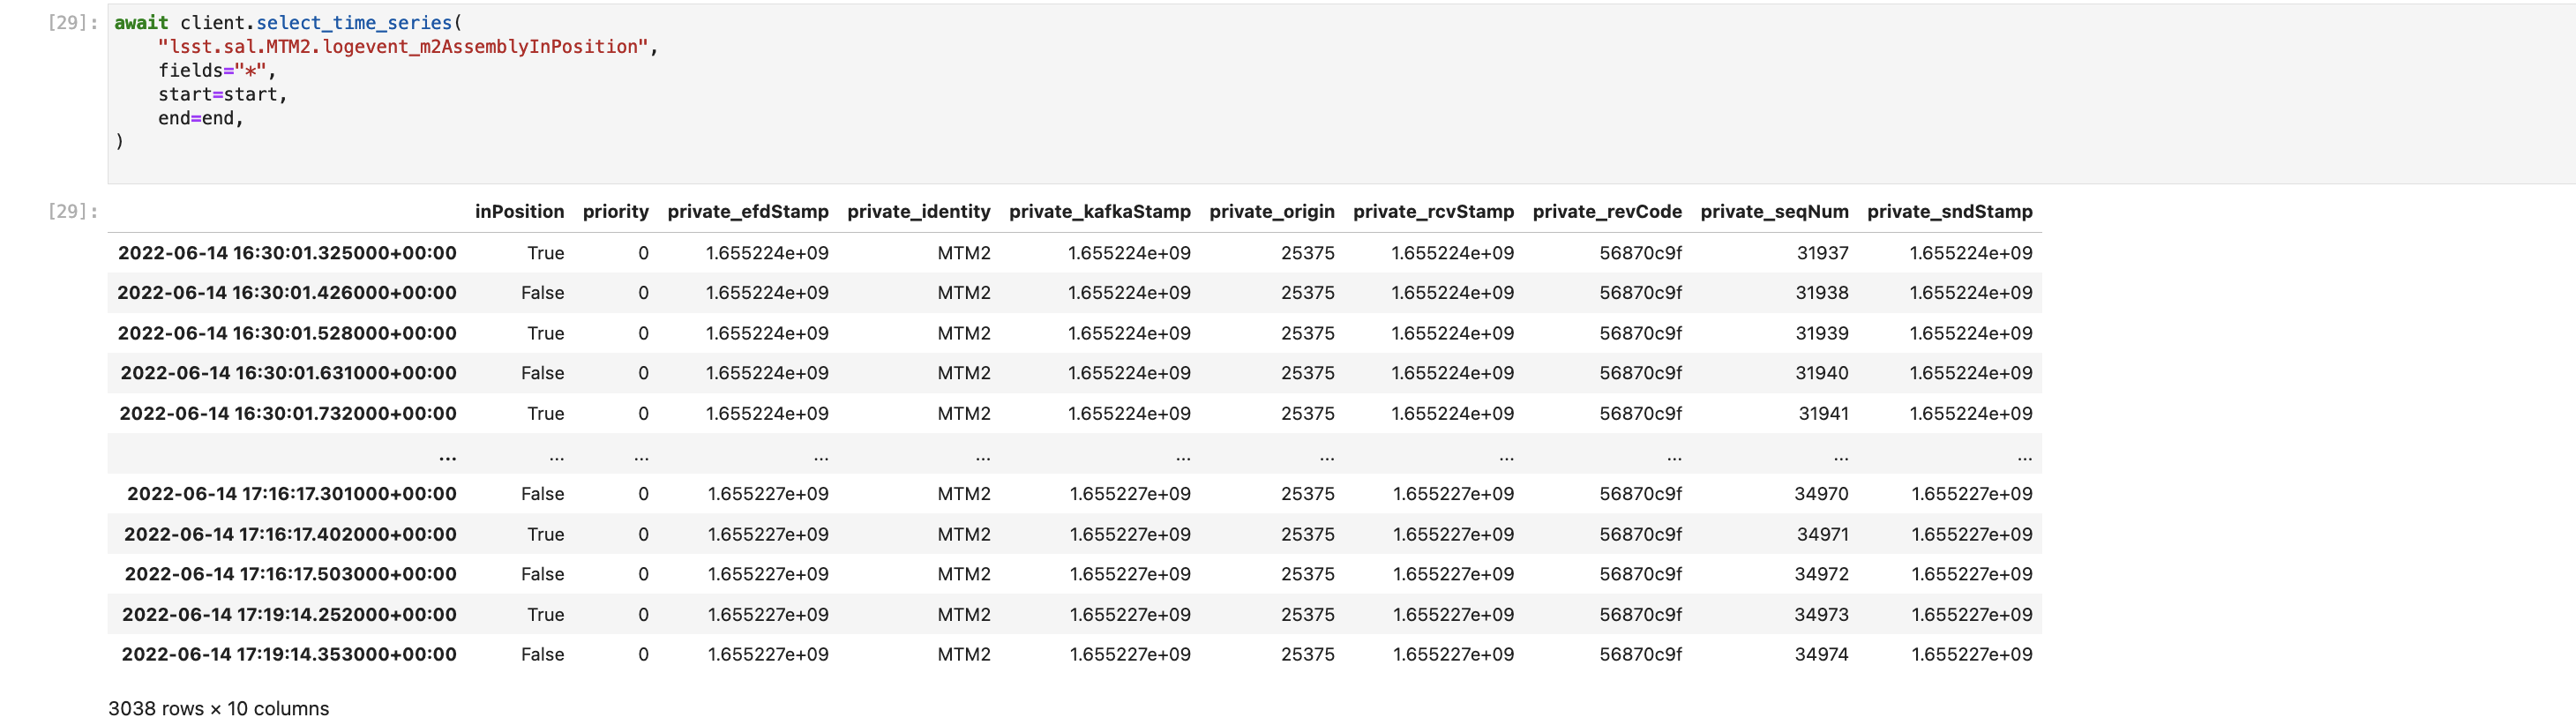
\includegraphics[width=3.12500in]{jira_imgs/2527.png}

}
\begin{tabular}{p{2cm}p{14cm}}
\toprule
Step 33 & Step Execution Status: \textbf{ Fail } \\ \hline
\end{tabular}
 Description \\
{\footnotesize
\textbf{Temperature Events}\\[2\baselineskip]Verify the
\emph{MTM2\_logevent\_CellTemperatureHiWarning and
\emph{MTM2\_logevent\_temperatureOffset}~}to the EFD

}
\hdashrule[0.5ex]{\textwidth}{1pt}{3mm}
  Expected Result \\
{\footnotesize
The \emph{MTM2\_logevent\_CellTemperatureHiWarning} publishes false and
the~\emph{MTM2\_logevent\_temperatureOffset}~is publishing values in the
EFD.

}
\hdashrule[0.5ex]{\textwidth}{1pt}{3mm}
  Actual Result \\
{\footnotesize
\emph{MTM2\_logevent\_CellTemperatureHiWarning~}is not publishing
anything in the test time window.\\
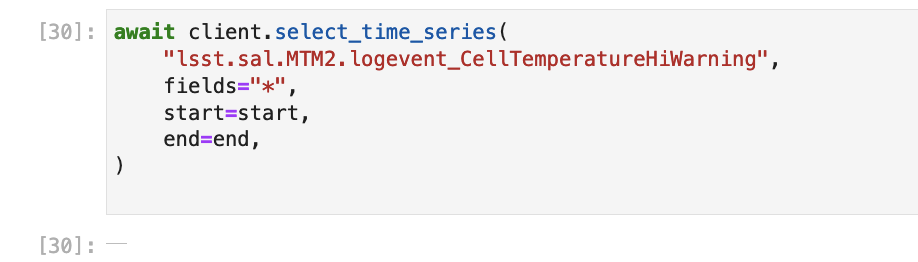
\includegraphics[width=3.12500in]{jira_imgs/2528.png}\\[2\baselineskip]​\emph{MTM2\_logevent\_temperatureOffset
is not publishing any data into the EFD}\\
\emph{\\
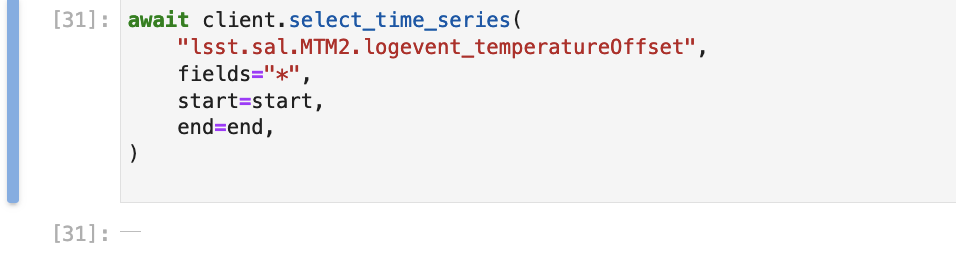
\includegraphics[width=3.12500in]{jira_imgs/2529.png}}\\

}
\begin{tabular}{p{2cm}p{14cm}}
\toprule
Step 34 & Step Execution Status: \textbf{ Fail } \\ \hline
\end{tabular}
 Description \\
{\footnotesize
\textbf{Interlock}\\
Verify the \emph{MTM2\_logevent\_interlock~}is published to the EFD.

}
\hdashrule[0.5ex]{\textwidth}{1pt}{3mm}
  Expected Result \\
{\footnotesize
The \emph{MTM2\_logevent\_interlock} event is published.

}
\hdashrule[0.5ex]{\textwidth}{1pt}{3mm}
  Actual Result \\
{\footnotesize
\emph{MTM2\_logevent\_interlock} not being published to the EFD.\\
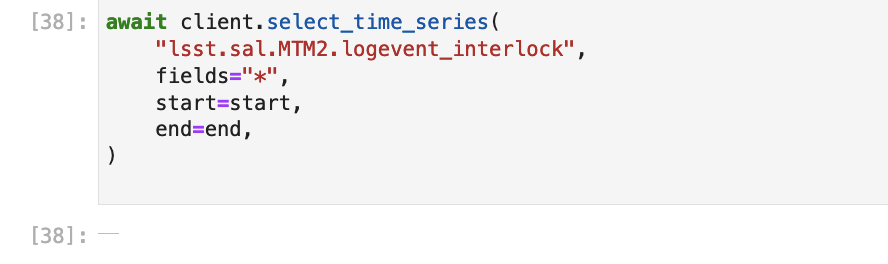
\includegraphics[width=3.12500in]{jira_imgs/2530.png}

}
\begin{tabular}{p{2cm}p{14cm}}
\toprule
Step 35 & Step Execution Status: \textbf{ Not Executed } \\ \hline
\end{tabular}
 Description \\
{\footnotesize
\textbf{TCP/IP connected\\
}\\
Unplug ethernet cable

}
\hdashrule[0.5ex]{\textwidth}{1pt}{3mm}
  Expected Result \\
{\footnotesize
The system will go into FAULT and a
\emph{MTM2\_logevent\_tcpIpConnected} event is published as FALSE.

}
\hdashrule[0.5ex]{\textwidth}{1pt}{3mm}
  Actual Result \\
{\footnotesize

}
\begin{tabular}{p{2cm}p{14cm}}
\toprule
Step 36 & Step Execution Status: \textbf{ Not Executed } \\ \hline
\end{tabular}
 Description \\
{\footnotesize
Plug ethernet cable back in.

}
\hdashrule[0.5ex]{\textwidth}{1pt}{3mm}
  Expected Result \\
{\footnotesize
The system is able to be moved out of FAULT state and the
\emph{MTM2\_logevent\_tcpIpConnected} event is true.

}
\hdashrule[0.5ex]{\textwidth}{1pt}{3mm}
  Actual Result \\
{\footnotesize

}
\begin{tabular}{p{2cm}p{14cm}}
\toprule
Step 37 & Step Execution Status: \textbf{ Fail } \\ \hline
\end{tabular}
 Description \\
{\footnotesize
\textbf{Hardpoint List}\\[2\baselineskip]Verify the
\emph{MTM2\_logevent\_hardpointList} is published to the EFD.

}
\hdashrule[0.5ex]{\textwidth}{1pt}{3mm}
  Test Data \\
 {\footnotesize
\textbf{{Note}}{: In HARRIS's original code, the hardpoint list was
hard-coded.}

}
\hdashrule[0.5ex]{\textwidth}{1pt}{3mm}
  Expected Result \\
{\footnotesize
The \emph{MTM2\_logevent\_hardpointList} is published based on the
actuator ID's.

}
\hdashrule[0.5ex]{\textwidth}{1pt}{3mm}
  Actual Result \\
{\footnotesize
\emph{MTM2\_logevent\_hardpointList not published to the EFD.~}\\
\emph{\\
}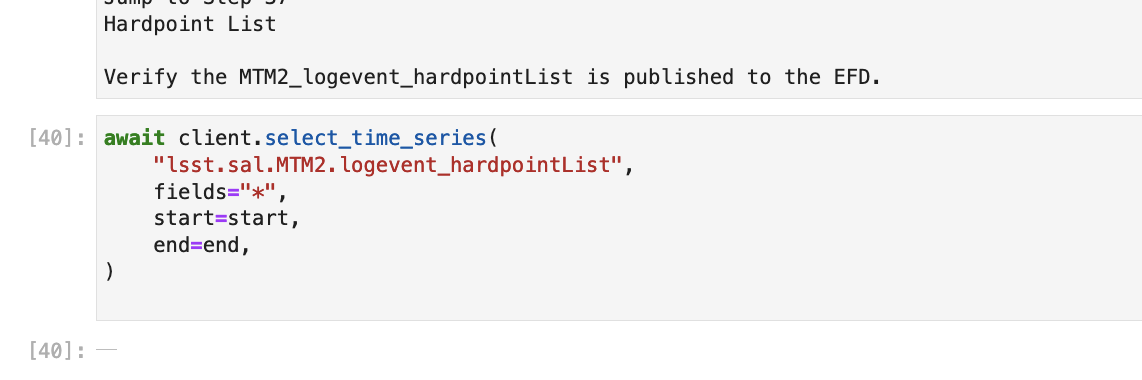
\includegraphics[width=3.12500in]{jira_imgs/2531.png}

}
\begin{tabular}{p{2cm}p{14cm}}
\toprule
Step 38 & Step Execution Status: \textbf{ Fail } \\ \hline
\end{tabular}
 Description \\
{\footnotesize
\textbf{Inclination Telemetry Source}\\[2\baselineskip]Verify the
\emph{MTM2\_logevent\_inclinationTelemetrySource} is published in the
EFD.

}
\hdashrule[0.5ex]{\textwidth}{1pt}{3mm}
  Expected Result \\
{\footnotesize
The \emph{MTM2\_logevent\_inclinationTelemetrySource} is published to
the EFD based on where the inclination telemetry is coming from.

}
\hdashrule[0.5ex]{\textwidth}{1pt}{3mm}
  Actual Result \\
{\footnotesize
Not seen in Chronograph, nor in a EFD query\\
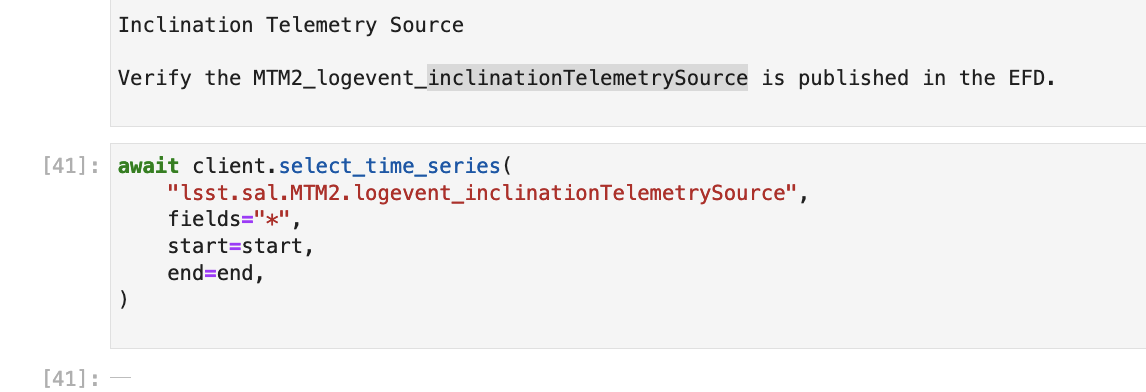
\includegraphics[width=3.12500in]{jira_imgs/2532.png}

}
\begin{tabular}{p{2cm}p{14cm}}
\toprule
Step 39 & Step Execution Status: \textbf{ Not Executed } \\ \hline
\end{tabular}
 Description \\
{\footnotesize
\textbf{Force Balance System Status}\\[2\baselineskip]Verify the
\emph{MTM2\_logevent\_forceBalanceSystemStatus} is being published to
the EFD.

}
\hdashrule[0.5ex]{\textwidth}{1pt}{3mm}
  Expected Result \\
{\footnotesize
The~\emph{MTM2\_logevent\_forceBalanceSystemStatus~}is published to the
EFD showing whether the FB system is on or off.

}
\hdashrule[0.5ex]{\textwidth}{1pt}{3mm}
  Actual Result \\
{\footnotesize
\emph{MTM2\_logevent\_forceBalanceSystemStatus is not being published to
the EFD}\\
\emph{\\
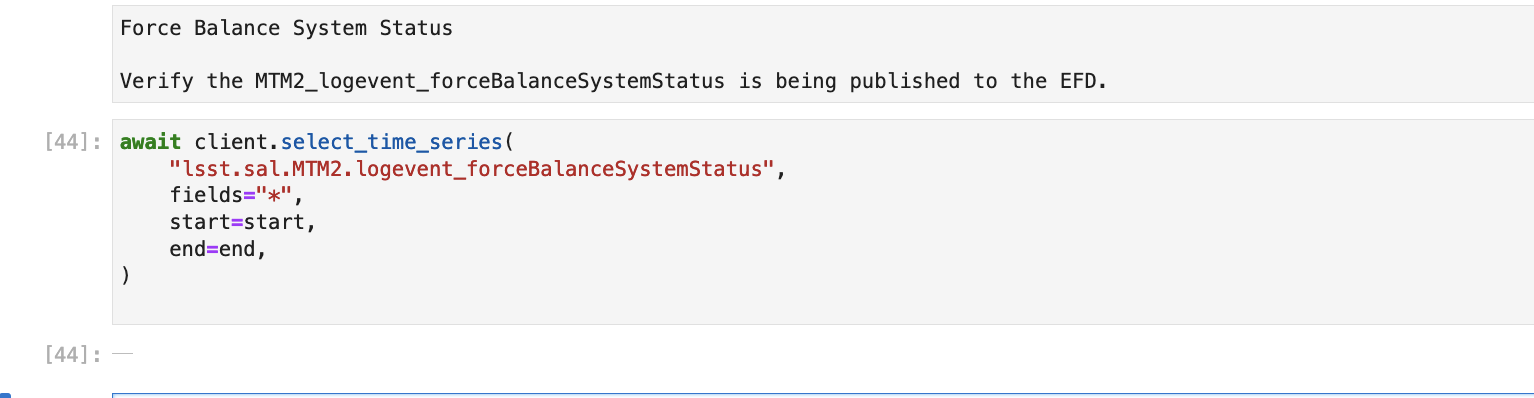
\includegraphics[width=3.12500in]{jira_imgs/2533.png}}\\

}
\begin{tabular}{p{2cm}p{14cm}}
\toprule
Step 40 & Step Execution Status: \textbf{ Initial Pass } \\ \hline
\end{tabular}
 Description \\
{\footnotesize
\textbf{ApplyForces command}\\[2\baselineskip]Before sending the
ApplyForces command, take note of the force telemetry output by the EFD.

}
\hdashrule[0.5ex]{\textwidth}{1pt}{3mm}
  Expected Result \\
{\footnotesize
The force telemetry should reflect the forces applied by the LUT. This
will be seen as the initial condition.

}
\hdashrule[0.5ex]{\textwidth}{1pt}{3mm}
  Actual Result \\
{\footnotesize
This plot shows the before and after sending the applyForces command
over SAL.\\
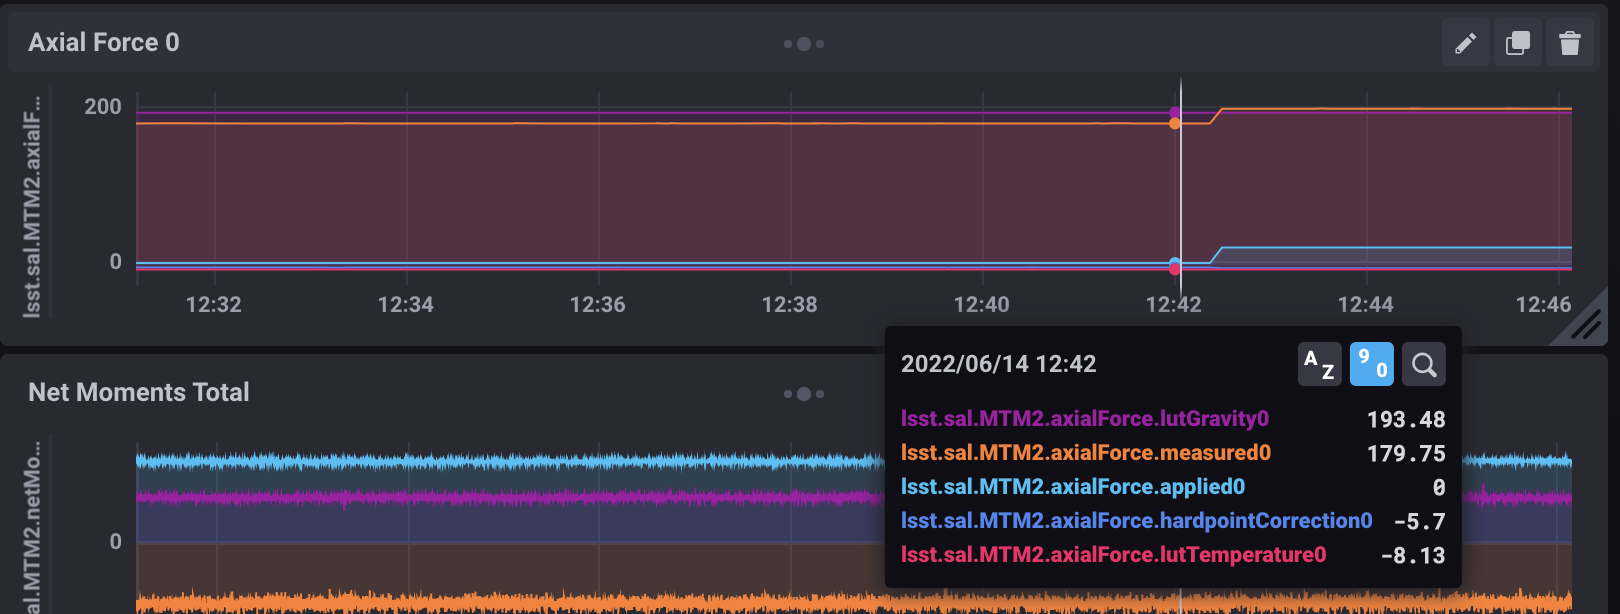
\includegraphics[width=6.53125in]{jira_imgs/2497.png}

}
\begin{tabular}{p{2cm}p{14cm}}
\toprule
Step 41 & Step Execution Status: \textbf{ Initial Pass } \\ \hline
\end{tabular}
 Description \\
{\footnotesize
In the Enabled State and closed-loop mode, send the \emph{ApplyForces}
command over SAL.

}
\hdashrule[0.5ex]{\textwidth}{1pt}{3mm}
  Test Data \\
 {\footnotesize
Force should not be applied to the axial actuators at the same time as
the tangential actuators. Make sure the summation of forces in the
Z-direction is zero. The forces applied should not be random values. As
an example, apply bending modes 1-20.

}
\hdashrule[0.5ex]{\textwidth}{1pt}{3mm}
  Expected Result \\
{\footnotesize
The force telemetry should show the combined value of forces from the
initial condition and the forces commanded through SAL. The difference
between the force telemetry between now and the initial condition should
equal the forces sent through the ApplyForces command.~

}
\hdashrule[0.5ex]{\textwidth}{1pt}{3mm}
  Actual Result \\
{\footnotesize
We ran this step 12 above when applying 20N to the B1 actuator.\\
This was done around 16:42 UTC.\\
You can see how the applied0 forces changed from 0 to 20N after the
command.

}
\begin{tabular}{p{2cm}p{14cm}}
\toprule
Step 42 & Step Execution Status: \textbf{ Initial Pass } \\ \hline
\end{tabular}
 Description \\
{\footnotesize
\textbf{ResetForceOffsets}\\[2\baselineskip]Send the
\emph{ResetForceOffsets} command through SAL.

}
\hdashrule[0.5ex]{\textwidth}{1pt}{3mm}
  Test Data \\
 {\footnotesize
This should be done after a successful ApplyForces command.~

}
\hdashrule[0.5ex]{\textwidth}{1pt}{3mm}
  Expected Result \\
{\footnotesize
Force telemetry should show a difference from when the ApplyForces
command was issued to after the resetforceoffsets command is issued. The
78 nonzero force values are now zero.~

}
\hdashrule[0.5ex]{\textwidth}{1pt}{3mm}
  Actual Result \\
{\footnotesize
This command was successful. The command was sent at around 17:04 UTC.\\
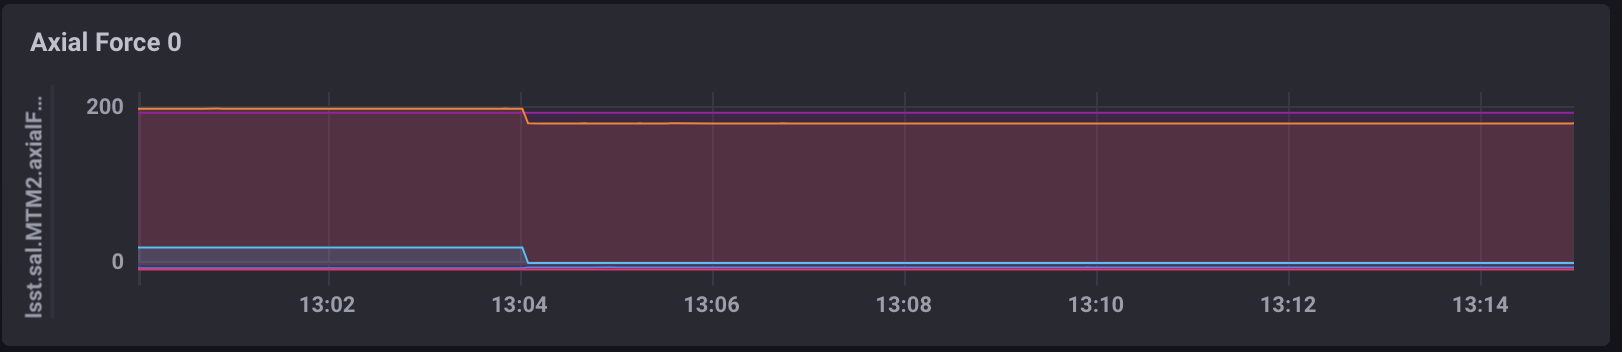
\includegraphics[width=6.60417in]{jira_imgs/2498.png}

}
\begin{tabular}{p{2cm}p{14cm}}
\toprule
Step 43 & Step Execution Status: \textbf{ Initial Pass } \\ \hline
\end{tabular}
 Description \\
{\footnotesize
\textbf{PositionMirror command}\\
{This is a dangerous step. This actuator can go out of the force range
and will be difficult to recover. This command is an engineering command
only. During observation, only the forces will be used as a measure to
move the mirror. See
https://jira.lsstcorp.org/secure/Tests.jspa\#/testPlayer/testExecution/LVV-E1008
for the limits.}\\
Axis are moved individually.\\[2\baselineskip]In the enabled state and
closed-loop mode, send a \emph{positionMirror} command of\\
P1= (100um,0,0,0,0,0)\\
P2= (0,100um,0,0,0,0)\\
P3= (0,0,100um,0,0,0)\\
P4= (0,0,0,100urad,0,0)\\
P5= (0,0,0,0,100urad,0)\\
P6= (0,0,0,0,0,100urad)

}
\hdashrule[0.5ex]{\textwidth}{1pt}{3mm}
  Test Data \\
 {\footnotesize
Note: There will be two types of telemetry - one measured by the
hardpoints and one measured by the IMS\\
This specific position was selected because it should be within the
limits so the positionMirror command can be verified without running
into an error.

}
\hdashrule[0.5ex]{\textwidth}{1pt}{3mm}
  Expected Result \\
{\footnotesize
\begin{itemize}
\tightlist
\item
  The telemetry data reported by the hardpoints and by the IMS is
  consistent to the position command given.~
\item
  The \emph{MTM2\_logevent\_m2AssemblyInPosition} event is published as
  true.
\end{itemize}

}
\hdashrule[0.5ex]{\textwidth}{1pt}{3mm}
  Actual Result \\
{\footnotesize
This step actually moves the mirror. We checked with Roberto Tighe that
confirmed that we can move it.\\[2\baselineskip]We were concerned about
any forces peaking up to more than a tolerated force so we only did
minor movements.\\
The mirror was at about x=21um and xRot=0.08 urad (and very small values
for y and z).\\
We could send the command to move the mirror to 0 on x, y, z, rotY. We
assume that rotZ and rotX are good.\\[2\baselineskip]The exploratory
test of checking the limits of how much we can move is out of the scope
of this test.

}
\begin{tabular}{p{2cm}p{14cm}}
\toprule
Step 44 & Step Execution Status: \textbf{ Initial Pass } \\ \hline
\end{tabular}
 Description \\
{\footnotesize
\textbf{ClearError command}\\
Unplug the cable to actuator A1.

}
\hdashrule[0.5ex]{\textwidth}{1pt}{3mm}
  Test Data \\
 {\footnotesize
A Mechanical Engineer must be present in order to unplug the actuator.

}
\hdashrule[0.5ex]{\textwidth}{1pt}{3mm}
  Expected Result \\
{\footnotesize
System goes into a ``FAULT'' state and is indicated by a red light on
the EUI.~

}
\hdashrule[0.5ex]{\textwidth}{1pt}{3mm}
  Actual Result \\
{\footnotesize
The low-level controller went to FAULT without any particular reason. We
did not investigate the reason for the failure but we confirmed that we
can clear the error using this command.

}
\begin{tabular}{p{2cm}p{14cm}}
\toprule
Step 45 & Step Execution Status: \textbf{ Initial Pass } \\ \hline
\end{tabular}
 Description \\
{\footnotesize
Send a \emph{clearErrors} command

}
\hdashrule[0.5ex]{\textwidth}{1pt}{3mm}
  Expected Result \\
{\footnotesize
the \emph{ClearErrors} command allows the system to transition out of
FAULT state and is able to re-enter Enabled/closed loop mode

}
\hdashrule[0.5ex]{\textwidth}{1pt}{3mm}
  Actual Result \\
{\footnotesize
As stated above, we sent the command and we could clear the error in the
low-level controller.

}
\begin{tabular}{p{2cm}p{14cm}}
\toprule
Step 46 & Step Execution Status: \textbf{ Not Executed } \\ \hline
\end{tabular}
 Description \\
{\footnotesize
\textbf{SwtichForceBalanceSystem command}\\
In the enabled state, send a \emph{switchForceBalanceSystem} command to
turn the FB system off.

}
\hdashrule[0.5ex]{\textwidth}{1pt}{3mm}
  Test Data \\
 {\footnotesize
Note: The Force Balance System is on by default.~

}
\hdashrule[0.5ex]{\textwidth}{1pt}{3mm}
  Expected Result \\
{\footnotesize
\begin{itemize}
\tightlist
\item
  The \emph{MTM2\_command\_switchForceBalanceSystem} is accepted and the
  FB system turns off.
\item
  The \emph{MTM2\_logevent\_forceBalanceSystemStatus~}event publishes
  false.
\end{itemize}

}
\hdashrule[0.5ex]{\textwidth}{1pt}{3mm}
  Actual Result \\
{\footnotesize
This command is not supported yet.~

}
\begin{tabular}{p{2cm}p{14cm}}
\toprule
Step 47 & Step Execution Status: \textbf{ Not Executed } \\ \hline
\end{tabular}
 Description \\
{\footnotesize
In the enabled state, send a \emph{switchForceBalanceSystem} command to
turn the FB system on.

}
\hdashrule[0.5ex]{\textwidth}{1pt}{3mm}
  Expected Result \\
{\footnotesize
\begin{itemize}
\tightlist
\item
  The \emph{MTM2\_command\_switchForceBalanceSystem} is accepted and the
  FB system turns on
\item
  The \emph{MTM2\_logevent\_forceBalanceSystemStatus~}event publishes
  true
\end{itemize}

}
\hdashrule[0.5ex]{\textwidth}{1pt}{3mm}
  Actual Result \\
{\footnotesize
This command is not supported yet.

}
\begin{tabular}{p{2cm}p{14cm}}
\toprule
Step 48 & Step Execution Status: \textbf{ Not Executed } \\ \hline
\end{tabular}
 Description \\
{\footnotesize
\textbf{SetTemperatureOffset command}\\
In the enabled state, send a \emph{setTemperatureOffset}command with the
following parameters:

\begin{itemize}
\tightlist
\item
  ring
\item
  intake
\item
  exhaust
\end{itemize}

}
\hdashrule[0.5ex]{\textwidth}{1pt}{3mm}
  Expected Result \\
{\footnotesize
\begin{itemize}
\tightlist
\item
  The \emph{MTM2\_command\_setTemperatureOffset} is accepted and the
  offset of the ring temperatures are changed.
\item
  The \emph{MTM2\_logevent\_temperatureOffset} event is updated given
  the new parameters
\end{itemize}

}
\hdashrule[0.5ex]{\textwidth}{1pt}{3mm}
  Actual Result \\
{\footnotesize
This command is not supported yet.

}
\begin{tabular}{p{2cm}p{14cm}}
\toprule
Step 49 & Step Execution Status: \textbf{ Not Executed } \\ \hline
\end{tabular}
 Description \\
{\footnotesize
\textbf{selectInclinationSource command}\\
In the enabled state, send a \emph{selectInclinationSource~}command to
choose the MTMount control system as the inclination source.

}
\hdashrule[0.5ex]{\textwidth}{1pt}{3mm}
  Test Data \\
 {\footnotesize
\textbf{Note:~}The default source is onboard.

}
\hdashrule[0.5ex]{\textwidth}{1pt}{3mm}
  Expected Result \\
{\footnotesize
\begin{itemize}
\tightlist
\item
  The source is changed to the MTMount Control System
\item
  The \emph{MTM2\_logevent\_inclinationTelemetrySource} event shows the
  MTMount Control system as the source.
\end{itemize}

}
\hdashrule[0.5ex]{\textwidth}{1pt}{3mm}
  Actual Result \\
{\footnotesize
This command is not supported yet.

}
\begin{tabular}{p{2cm}p{14cm}}
\toprule
Step 50 & Step Execution Status: \textbf{ Not Executed } \\ \hline
\end{tabular}
 Description \\
{\footnotesize
In the enabled state, send a \emph{selectInclinationSource~}command to
select the inclination source as onboard.

}
\hdashrule[0.5ex]{\textwidth}{1pt}{3mm}
  Expected Result \\
{\footnotesize
\begin{itemize}
\tightlist
\item
  The source is changed to onboard
\item
  The\emph{~MTM2\_logevent\_inclinationTelemetrySource~}event shows
  onboard as the source.
\end{itemize}

}
\hdashrule[0.5ex]{\textwidth}{1pt}{3mm}
  Actual Result \\
{\footnotesize
This command is not supported yet.

}

\paragraph{ LVV-T1600 - Integration of Camera Hexapod with SAL }\mbox{}\\

Version \textbf{2}.
Open  \href{https://jira.lsstcorp.org/secure/Tests.jspa#/testCase/LVV-T1600}{\textit{ LVV-T1600 } }
test case in Jira.

The objective of this test case is to re-verify the functional
requirements of the camera hexapod's software, after shipment of the
hardware from the vendor's facility to the Summit, as defined in \citeds{LTS-206}
and \citeds{LTS-160}. This test case will only exercise the functionality that
was executed previously and meets the following criteria:

\begin{itemize}
\tightlist
\item
  Only requires the use of Russell's code to replace MOOG's middleware
  code
\item
  Only requires the camera hexapod to be operable
\item
  Only requires command through the CSC after the cRIO is switched from
  GUI mode to DDS mode
\item
  Only requires testing of the synchronous mode

  \begin{itemize}
  \tightlist
  \item
    \textbf{Asynchronous mode is not a standard mode of operation}
  \end{itemize}
\item
  This test case can be executed with or without the camera rotator to
  be loaded with the camera simulated mass or actual camera hardware
\end{itemize}

The software functional requirements were previously verified during the
test campaign by the vendor at the vendor's facility and accepted by
LSST during the Factory Acceptance Test review. The test procedure used
during the vendor's acceptance testing is the \emph{LSST
Hexapods-Rotator Software Acceptance Test Procedure} which is attached
to this test case. The test steps of this test case are derived from the
same procedure, but the order of the steps have been changed to reflect
the \emph{Proposal of Hexapod Test~on Dec. 2019~}Confluence page which
can be found linked in the Traceability tab.\\[2\baselineskip]See the
attached \emph{LSST Rotator Hexapod's Manual} for more information on
how to operate the hexapod.

\textbf{ Preconditions}:\\
Prior to the execution of this test case to re-verify the Camera Hexapod
hardware functional requirements, the following Summit tasks must be
completed:

\begin{itemize}
\tightlist
\item
  The Hexapod has been installed on the camera cart

  \begin{itemize}
  \tightlist
  \item
    \url{https://jira.lsstcorp.org/browse/SUMMIT-3224}
  \end{itemize}
\item
  The Hexapod Controller has been deployed on the summit

  \begin{itemize}
  \tightlist
  \item
    \url{https://jira.lsstcorp.org/browse/SUMMIT-3229}
  \end{itemize}
\item
  Boxes for the Hexapod have been transported to the 3rd level

  \begin{itemize}
  \tightlist
  \item
    \url{https://jira.lsstcorp.org/browse/SUMMIT-3230}
  \end{itemize}
\item
  All Hexapod cables and cabinets have been prepared for integration
  with camera cart

  \begin{itemize}
  \tightlist
  \item
    \url{https://jira.lsstcorp.org/browse/SUMMIT-3231}
  \end{itemize}
\item
  The offset has been installed onto the integrating structure

  \begin{itemize}
  \tightlist
  \item
    \url{https://jira.lsstcorp.org/browse/SUMMIT-3293}
  \end{itemize}
\item
  The Camera Hexapod electrical connections have been tested

  \begin{itemize}
  \tightlist
  \item
    \url{https://jira.lsstcorp.org/browse/SUMMIT-3294}
  \end{itemize}
\end{itemize}

Execution status: {\bf Not Executed }

Final comment:\\


Detailed steps results:

\begin{tabular}{p{2cm}p{14cm}}
\toprule
Step 1 & Step Execution Status: \textbf{ Not Executed } \\ \hline
\end{tabular}
 Description \\
{\footnotesize
\textbf{STARTING THE EUI}\\[2\baselineskip]Double click the Hexapod GUI
Viewer desktop icon on the computer.

\begin{itemize}
\tightlist
\item
  This can be done on the Dell Management PC or another computer on the
  same network
\end{itemize}

}
\hdashrule[0.5ex]{\textwidth}{1pt}{3mm}
  Expected Result \\
{\footnotesize
A prompt to enter a password is shown.~

}
\hdashrule[0.5ex]{\textwidth}{1pt}{3mm}
  Actual Result \\
{\footnotesize

}
\begin{tabular}{p{2cm}p{14cm}}
\toprule
Step 2 & Step Execution Status: \textbf{ Not Executed } \\ \hline
\end{tabular}
 Description \\
{\footnotesize
Enter the password ``lsst-vnc''

\begin{itemize}
\tightlist
\item
  If the EUI isn't automatically up and running when the VNC opens,
  double click on the Hexapod-eGUI icon on the VNC viewer
\end{itemize}

}
\hdashrule[0.5ex]{\textwidth}{1pt}{3mm}
  Expected Result \\
{\footnotesize
The EUI is in the Offline State/PublishOnly substate and is able to
publish through SAL but cannot receive commands.

}
\hdashrule[0.5ex]{\textwidth}{1pt}{3mm}
  Actual Result \\
{\footnotesize

}
\begin{tabular}{p{2cm}p{14cm}}
\toprule
Step 3 & Step Execution Status: \textbf{ Not Executed } \\ \hline
\end{tabular}
 Description \\
{\footnotesize
\textbf{OFFLINESTATE/PUBLISHONLY -\textgreater{}
OFFLINESTATE/AVAILABLESTATE}\\
On the Main tab, select the ``Offline SubState Cmd'' field in the
Commands to Send section, set the Offline SubState Triggers to ``System
Ready'' and click on the Send Command button.\\
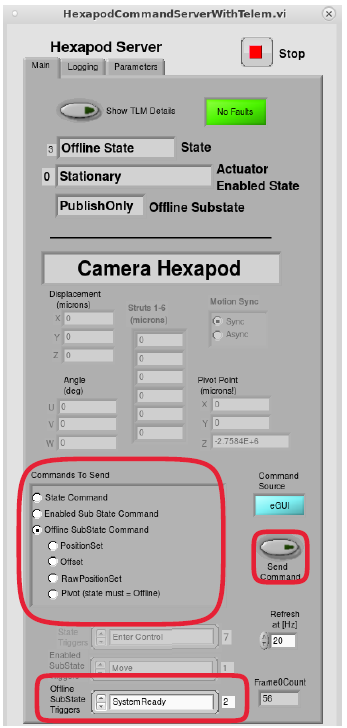
\includegraphics[width=1.79167in]{jira_imgs/1024.png}

}
\hdashrule[0.5ex]{\textwidth}{1pt}{3mm}
  Expected Result \\
{\footnotesize
The system transitions from the OfflineState/PublishOnly substate to the
OfflineState/AvailableState substate.\\[2\baselineskip]

}
\hdashrule[0.5ex]{\textwidth}{1pt}{3mm}
  Actual Result \\
{\footnotesize

}
\begin{tabular}{p{2cm}p{14cm}}
\toprule
Step 4 & Step Execution Status: \textbf{ Not Executed } \\ \hline
\end{tabular}
 Description \\
{\footnotesize
\textbf{SWITCHING TO DDS MODE}\\
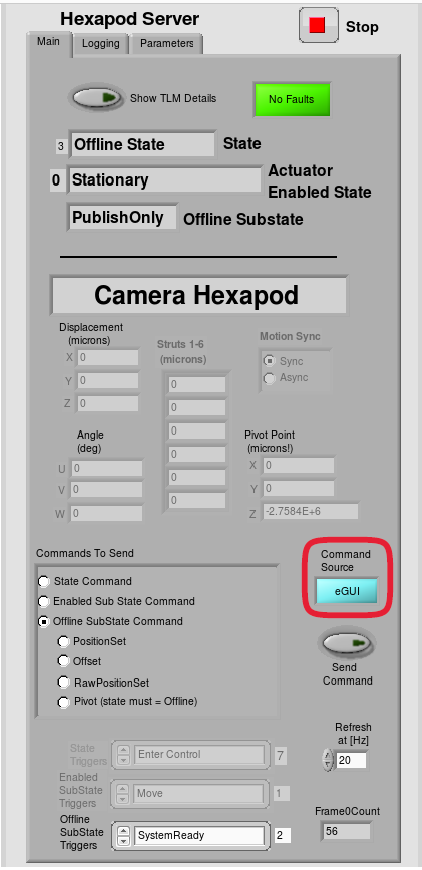
\includegraphics[width=1.68750in]{jira_imgs/1025.png}If the Command
Source does not show DDS, go to the Parameters tab, select DDS under the
Command Source and click the Set Cmd Source button.\\
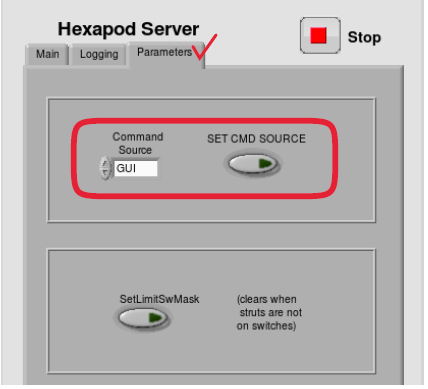
\includegraphics[width=2.34375in]{jira_imgs/1026.png}\textbf{Note:~If
the GUI is used after being set to DDS mode, the system will switch back
the Command Source to GUI and ignore any DDS commands. The Command
Source must show DDS in order to receive DDS commands.}

}
\hdashrule[0.5ex]{\textwidth}{1pt}{3mm}
  Expected Result \\
{\footnotesize
The system is capable of receiving/responding to DDS commands.

}
\hdashrule[0.5ex]{\textwidth}{1pt}{3mm}
  Actual Result \\
{\footnotesize

}
\begin{tabular}{p{2cm}p{14cm}}
\toprule
Step 5 & Step Execution Status: \textbf{ Not Executed } \\ \hline
\end{tabular}
 Description \\
{\footnotesize
\textbf{OFFLINESTATE -\textgreater{} STANDBYSTATE}\\
The system receives an enterControl State Transition command through
DDS.

}
\hdashrule[0.5ex]{\textwidth}{1pt}{3mm}
  Expected Result \\
{\footnotesize
The system transitions into the StandbyState and is capable of
receiving/responding to DDS commands.

}
\hdashrule[0.5ex]{\textwidth}{1pt}{3mm}
  Actual Result \\
{\footnotesize

}
\begin{tabular}{p{2cm}p{14cm}}
\toprule
Step 6 & Step Execution Status: \textbf{ Not Executed } \\ \hline
\end{tabular}
 Description \\
{\footnotesize
\textbf{STANDBYSTATE -\textgreater{} DISABLEDSTATE}\\
From the StandbyState, send a start command through the DDS.

}
\hdashrule[0.5ex]{\textwidth}{1pt}{3mm}
  Expected Result \\
{\footnotesize
The system transitions into DisabledState after receiving/responding to
DDS command and the wrapper in the PXI real time controller looks for
the configuration file.\\[2\baselineskip]If the configuration file is
invalid or out of range, the system will transition into a Fault State

}
\hdashrule[0.5ex]{\textwidth}{1pt}{3mm}
  Actual Result \\
{\footnotesize

}
\begin{tabular}{p{2cm}p{14cm}}
\toprule
Step 7 & Step Execution Status: \textbf{ Not Executed } \\ \hline
\end{tabular}
 Description \\
{\footnotesize
\textbf{DISABLEDSTATE -\textgreater{} ENABLEDSTATE}\\
From the DisabledState, send an enable state command through the DDS.\\
\textbf{}

}
\hdashrule[0.5ex]{\textwidth}{1pt}{3mm}
  Expected Result \\
{\footnotesize
The system transitions into the EnabledState/Stationary substate, the
motor drives are enabled, motor brakes are released and the system is
capable of receiving/responding to DDS commands.\\[2\baselineskip]

}
\hdashrule[0.5ex]{\textwidth}{1pt}{3mm}
  Actual Result \\
{\footnotesize

}
\begin{tabular}{p{2cm}p{14cm}}
\toprule
Step 8 & Step Execution Status: \textbf{ Not Executed } \\ \hline
\end{tabular}
 Description \\
{\footnotesize
\textbf{FAULTSTATE}\\
If a Fault occurs in any of the other states, the system will
automatically transition to the Fault State. While in the Fault state,
send a clearError command through the DDS.\\
Note: If the fault that occurs goes through the interlock system, reset
the safety relay switch and send a clearError command.

}
\hdashrule[0.5ex]{\textwidth}{1pt}{3mm}
  Expected Result \\
{\footnotesize
The system transitions back to the OfflineState/PublishOnly substate and
is not capable of receiving/responding to DDS commands. (Go back to Step
3)

}
\hdashrule[0.5ex]{\textwidth}{1pt}{3mm}
  Actual Result \\
{\footnotesize

}
\begin{tabular}{p{2cm}p{14cm}}
\toprule
Step 9 & Step Execution Status: \textbf{ Not Executed } \\ \hline
\end{tabular}
 Description \\
{\footnotesize
Verify the Hexapod is commandable by DDS by checking the EFD.

}
\hdashrule[0.5ex]{\textwidth}{1pt}{3mm}
  Expected Result \\
{\footnotesize
The \emph{MTHexapod\_logevent\_commandableByDDS} publishes true.

}
\hdashrule[0.5ex]{\textwidth}{1pt}{3mm}
  Actual Result \\
{\footnotesize

}
\begin{tabular}{p{2cm}p{14cm}}
\toprule
Step 10 & Step Execution Status: \textbf{ Not Executed } \\ \hline
\end{tabular}
 Description \\
{\footnotesize
Verify the TCP/IP is connected to the low level controller.

}
\hdashrule[0.5ex]{\textwidth}{1pt}{3mm}
  Expected Result \\
{\footnotesize
The \emph{MTHexapod\_logevent\_connected} publishes true.

}
\hdashrule[0.5ex]{\textwidth}{1pt}{3mm}
  Actual Result \\
{\footnotesize

}
\begin{tabular}{p{2cm}p{14cm}}
\toprule
Step 11 & Step Execution Status: \textbf{ Not Executed } \\ \hline
\end{tabular}
 Description \\
{\footnotesize
Verify the \emph{MTHexapod\_logevent\_configuration} event is publishing
data to the EFD.

}
\hdashrule[0.5ex]{\textwidth}{1pt}{3mm}
  Expected Result \\
{\footnotesize
The \emph{MTHexapod\_logevent\_configuration} is publishing reasonable
values.

}
\hdashrule[0.5ex]{\textwidth}{1pt}{3mm}
  Actual Result \\
{\footnotesize

}
\begin{tabular}{p{2cm}p{14cm}}
\toprule
Step 12 & Step Execution Status: \textbf{ Not Executed } \\ \hline
\end{tabular}
 Description \\
{\footnotesize
Verify the \emph{MTHexapod\_logevent\_interlock} event is publishing
data to the EFD.

}
\hdashrule[0.5ex]{\textwidth}{1pt}{3mm}
  Expected Result \\
{\footnotesize
The \emph{MTHexapod\_logevent\_interlock} is publishing and shows no
safety interlock is engaged.

}
\hdashrule[0.5ex]{\textwidth}{1pt}{3mm}
  Actual Result \\
{\footnotesize

}
\begin{tabular}{p{2cm}p{14cm}}
\toprule
Step 13 & Step Execution Status: \textbf{ Not Executed } \\ \hline
\end{tabular}
 Description \\
{\footnotesize
Verify that the thermal sensors are connected and producing telemetry
into the EFD.

}
\hdashrule[0.5ex]{\textwidth}{1pt}{3mm}
  Expected Result \\
{\footnotesize
All actuator temperatures are published to the EFD.

}
\hdashrule[0.5ex]{\textwidth}{1pt}{3mm}
  Actual Result \\
{\footnotesize

}
\begin{tabular}{p{2cm}p{14cm}}
\toprule
Step 14 & Step Execution Status: \textbf{ Not Executed } \\ \hline
\end{tabular}
 Description \\
{\footnotesize
The following steps define what the Jupyter Notebook for this test case
implements. Executing the Jupyter notebook is the only actual command
and control step that needs to be executed.

}
\hdashrule[0.5ex]{\textwidth}{1pt}{3mm}
  Expected Result \\
{\footnotesize
The Jupyter notebook controls the system to run through the steps below.

}
\hdashrule[0.5ex]{\textwidth}{1pt}{3mm}
  Actual Result \\
{\footnotesize

}
\begin{tabular}{p{2cm}p{14cm}}
\toprule
Step 15 & Step Execution Status: \textbf{ Not Executed } \\ \hline
\end{tabular}
 Description \\
{\footnotesize
Verify the \emph{MTHexapod\_actautors~}data is being published to the
EFD.

}
\hdashrule[0.5ex]{\textwidth}{1pt}{3mm}
  Expected Result \\
{\footnotesize
The actuators telemetry is being ingested into the EFD.

}
\hdashrule[0.5ex]{\textwidth}{1pt}{3mm}
  Actual Result \\
{\footnotesize

}
\begin{tabular}{p{2cm}p{14cm}}
\toprule
Step 16 & Step Execution Status: \textbf{ Not Executed } \\ \hline
\end{tabular}
 Description \\
{\footnotesize
Verify the \emph{MTHexapod\_application~}data is being published to the
EFD.

}
\hdashrule[0.5ex]{\textwidth}{1pt}{3mm}
  Expected Result \\
{\footnotesize
The application telemetry is being ingested into the EFD.

}
\hdashrule[0.5ex]{\textwidth}{1pt}{3mm}
  Actual Result \\
{\footnotesize

}
\begin{tabular}{p{2cm}p{14cm}}
\toprule
Step 17 & Step Execution Status: \textbf{ Not Executed } \\ \hline
\end{tabular}
 Description \\
{\footnotesize
Verify the \emph{MTHexapod\_electrical~}data is being published to the
EFD.

}
\hdashrule[0.5ex]{\textwidth}{1pt}{3mm}
  Expected Result \\
{\footnotesize
\emph{}The electrical telemetry is being ingested into the EFD.

}
\hdashrule[0.5ex]{\textwidth}{1pt}{3mm}
  Actual Result \\
{\footnotesize

}
\begin{tabular}{p{2cm}p{14cm}}
\toprule
Step 18 & Step Execution Status: \textbf{ Not Executed } \\ \hline
\end{tabular}
 Description \\
{\footnotesize
\textbf{{MOVE TEST}}\\
\textbf{Section 3.1.2 of the attached Software Acceptance Test
Procedure\\
Test Sequence \#1 - Synchronous Move Commands}\\
With the synchronous button enabled and in enabled/stationary state,
send a \emph{move} command of (x= 500um, y= -500um, z=200um, u=0.01deg,
v=-0.015deg, w=0deg).

}
\hdashrule[0.5ex]{\textwidth}{1pt}{3mm}
  Expected Result \\
{\footnotesize
\begin{itemize}
\tightlist
\item
  The hexapod moves to (x= 500um,y= -500um, z=200um, u=0.01deg,
  v=-0.015deg, w=0deg)
\item
  Since the Hexapod is in synchronous mode, the actuators complete the
  move at nearly the same time.
\end{itemize}

}
\hdashrule[0.5ex]{\textwidth}{1pt}{3mm}
  Actual Result \\
{\footnotesize

}
\begin{tabular}{p{2cm}p{14cm}}
\toprule
Step 19 & Step Execution Status: \textbf{ Not Executed } \\ \hline
\end{tabular}
 Description \\
{\footnotesize
Record the corresponding DDS events that were generated.

}
\hdashrule[0.5ex]{\textwidth}{1pt}{3mm}
  Expected Result \\
{\footnotesize
\begin{itemize}
\tightlist
\item
  The controllerState.enabledSubstate goes to MOVING\_POINT\_TO\_POINT
  when the move begins and STATIONARY when the move ends.
\item
  An \emph{inPosition} event is generated when the move is complete
\end{itemize}

}
\hdashrule[0.5ex]{\textwidth}{1pt}{3mm}
  Actual Result \\
{\footnotesize

}
\begin{tabular}{p{2cm}p{14cm}}
\toprule
Step 20 & Step Execution Status: \textbf{ Not Executed } \\ \hline
\end{tabular}
 Description \\
{\footnotesize
Wait 39 seconds.

}
\hdashrule[0.5ex]{\textwidth}{1pt}{3mm}
  Expected Result \\
{\footnotesize

}
\hdashrule[0.5ex]{\textwidth}{1pt}{3mm}
  Actual Result \\
{\footnotesize

}
\begin{tabular}{p{2cm}p{14cm}}
\toprule
Step 21 & Step Execution Status: \textbf{ Not Executed } \\ \hline
\end{tabular}
 Description \\
{\footnotesize
Record the corresponding thermal sensors and verify they are below 19
deg C. If they are above 19 deg C, wait until they are below 19 deg C to
perform the following steps.

}
\hdashrule[0.5ex]{\textwidth}{1pt}{3mm}
  Expected Result \\
{\footnotesize
All actuators are below 19 deg C.

}
\hdashrule[0.5ex]{\textwidth}{1pt}{3mm}
  Actual Result \\
{\footnotesize

}
\begin{tabular}{p{2cm}p{14cm}}
\toprule
Step 22 & Step Execution Status: \textbf{ Not Executed } \\ \hline
\end{tabular}
 Description \\
{\footnotesize
\textbf{Section 3.1.2 of the attached Software Acceptance Test
Procedure\\
Test Sequence \#5 - Stop Commands}\\
In the enabled/stationary state, send a move command of (x=0um, y=0um,
z=5000um, u=0deg, v=0deg, w=0deg)

}
\hdashrule[0.5ex]{\textwidth}{1pt}{3mm}
  Expected Result \\
{\footnotesize
The hexapod begins to move.

}
\hdashrule[0.5ex]{\textwidth}{1pt}{3mm}
  Actual Result \\
{\footnotesize

}
\begin{tabular}{p{2cm}p{14cm}}
\toprule
Step 23 & Step Execution Status: \textbf{ Not Executed } \\ \hline
\end{tabular}
 Description \\
{\footnotesize
Wait 3s.

}
\hdashrule[0.5ex]{\textwidth}{1pt}{3mm}
  Expected Result \\
{\footnotesize
The hexapod is still moving.

}
\hdashrule[0.5ex]{\textwidth}{1pt}{3mm}
  Actual Result \\
{\footnotesize

}
\begin{tabular}{p{2cm}p{14cm}}
\toprule
Step 24 & Step Execution Status: \textbf{ Not Executed } \\ \hline
\end{tabular}
 Description \\
{\footnotesize
Send a stop command.

}
\hdashrule[0.5ex]{\textwidth}{1pt}{3mm}
  Expected Result \\
{\footnotesize
The hexapod stops before reaching the previously commanded position

}
\hdashrule[0.5ex]{\textwidth}{1pt}{3mm}
  Actual Result \\
{\footnotesize

}
\begin{tabular}{p{2cm}p{14cm}}
\toprule
Step 25 & Step Execution Status: \textbf{ Not Executed } \\ \hline
\end{tabular}
 Description \\
{\footnotesize
Record the corresponding DDS events that were generated.

}
\hdashrule[0.5ex]{\textwidth}{1pt}{3mm}
  Expected Result \\
{\footnotesize
\begin{itemize}
\tightlist
\item
  The controllerState.enabledSubstate goes to CONTROLLED\_STOPPING when
  the stop is requested, then STATIONARY when the hexapod has halted.
\item
  In the EFD the codes for the EnabledSubstate are:

  \begin{itemize}
  \tightlist
  \item
    Stationary=0
  \item
    MovingPointToPoint=1
  \item
    SlewingOrTracking=2
  \item
    ControlledStopping=3
  \item
    Initializing=4
  \item
    Relative=5
  \item
    ConstantVelocity=6
  \end{itemize}
\item
  No \emph{inPosition} event is generated.
\end{itemize}

}
\hdashrule[0.5ex]{\textwidth}{1pt}{3mm}
  Actual Result \\
{\footnotesize

}
\begin{tabular}{p{2cm}p{14cm}}
\toprule
Step 26 & Step Execution Status: \textbf{ Not Executed } \\ \hline
\end{tabular}
 Description \\
{\footnotesize
Wait 39 seconds.

}
\hdashrule[0.5ex]{\textwidth}{1pt}{3mm}
  Expected Result \\
{\footnotesize

}
\hdashrule[0.5ex]{\textwidth}{1pt}{3mm}
  Actual Result \\
{\footnotesize

}
\begin{tabular}{p{2cm}p{14cm}}
\toprule
Step 27 & Step Execution Status: \textbf{ Not Executed } \\ \hline
\end{tabular}
 Description \\
{\footnotesize
Record the corresponding thermal sensors and verify they are below 19
deg C. If they are above 19 deg C, wait until they are below 19 deg C to
perform the following steps.

}
\hdashrule[0.5ex]{\textwidth}{1pt}{3mm}
  Expected Result \\
{\footnotesize
All actuators are below 19 deg C.

}
\hdashrule[0.5ex]{\textwidth}{1pt}{3mm}
  Actual Result \\
{\footnotesize

}
\begin{tabular}{p{2cm}p{14cm}}
\toprule
Step 28 & Step Execution Status: \textbf{ Not Executed } \\ \hline
\end{tabular}
 Description \\
{\footnotesize
\textbf{Test the ``setCompensationMode'' command.}\\[2\baselineskip]In
enabled/stationary state, send a \emph{move} command of (x=0um, y=0um,
z=800um, u=0deg, v=0deg, w=0deg)\\[2\baselineskip]

}
\hdashrule[0.5ex]{\textwidth}{1pt}{3mm}
  Expected Result \\
{\footnotesize
The hexapod moves to the position (x=0um, y=0um, z=800um, u=0deg,
v=0deg, w=0deg) and, since we are moving in synchronous mode, the
actuators complete the move at nearly the same time.

}
\hdashrule[0.5ex]{\textwidth}{1pt}{3mm}
  Actual Result \\
{\footnotesize

}
\begin{tabular}{p{2cm}p{14cm}}
\toprule
Step 29 & Step Execution Status: \textbf{ Not Executed } \\ \hline
\end{tabular}
 Description \\
{\footnotesize
Ensure that MTMount publishes the telescope elevation angle and
MTRotator publishes the rotation angle of the rotator. Either as real
components or through controllers simulating the components.

}
\hdashrule[0.5ex]{\textwidth}{1pt}{3mm}
  Expected Result \\
{\footnotesize
Published telescope elevation and rotator angle.

}
\hdashrule[0.5ex]{\textwidth}{1pt}{3mm}
  Actual Result \\
{\footnotesize

}
\begin{tabular}{p{2cm}p{14cm}}
\toprule
Step 30 & Step Execution Status: \textbf{ Not Executed } \\ \hline
\end{tabular}
 Description \\
{\footnotesize
In enabled/stationary state, send a ~\emph{setCompensationMode} command
to enable compensation.

}
\hdashrule[0.5ex]{\textwidth}{1pt}{3mm}
  Expected Result \\
{\footnotesize
The hexapod does not move and the
~\emph{MTHexapod\_logevent\_compensationMode} event appears as true in
the EFD.\\[2\baselineskip]The
\emph{MTHexapod\_logevent\_compensatedPosition} is also sent to the EFD.

}
\hdashrule[0.5ex]{\textwidth}{1pt}{3mm}
  Actual Result \\
{\footnotesize

}
\begin{tabular}{p{2cm}p{14cm}}
\toprule
Step 31 & Step Execution Status: \textbf{ Not Executed } \\ \hline
\end{tabular}
 Description \\
{\footnotesize
In enabled/stationary state, send a \emph{move} command of (0um, 0um,
800um, 0deg, 0deg, 0deg)

}
\hdashrule[0.5ex]{\textwidth}{1pt}{3mm}
  Expected Result \\
{\footnotesize
The hexapod moves to a slightly different position than (0um, 0um,
800um, 0deg, 0deg, 0deg) and, since we are moving in synchronous mode,
the actuators complete the move at nearly the same time.

}
\hdashrule[0.5ex]{\textwidth}{1pt}{3mm}
  Actual Result \\
{\footnotesize

}
\begin{tabular}{p{2cm}p{14cm}}
\toprule
Step 32 & Step Execution Status: \textbf{ Not Executed } \\ \hline
\end{tabular}
 Description \\
{\footnotesize
Check if there are any different events between move with and without
setCompensationMode=True. Check the movement in the EFD use:\\
Compare logevent\_compensatedPosition to logevent\_uncompensatedPosition

}
\hdashrule[0.5ex]{\textwidth}{1pt}{3mm}
  Expected Result \\
{\footnotesize
The changes are expected according to this table:\\
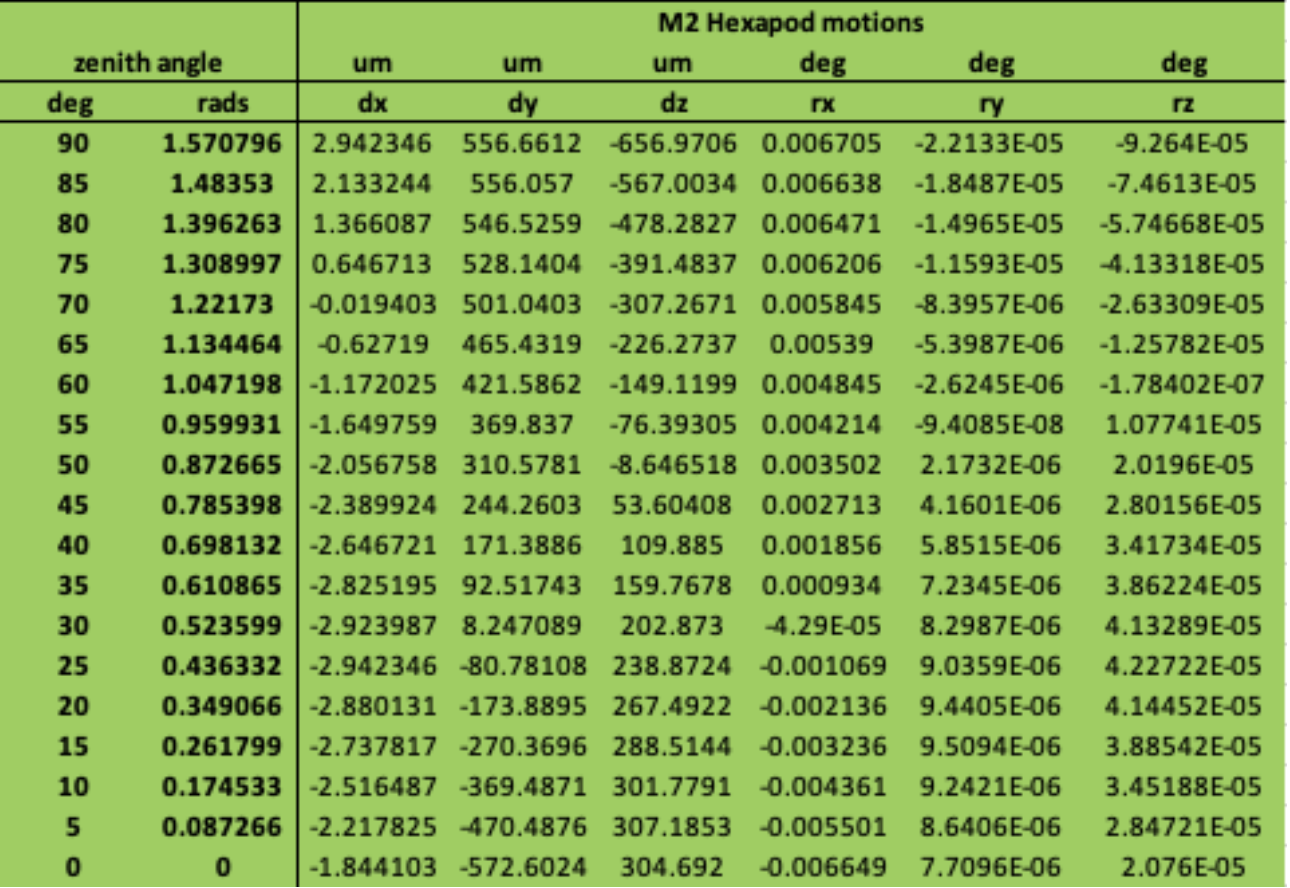
\includegraphics[width=1.56250in]{jira_imgs/1620.png}\\

}
\hdashrule[0.5ex]{\textwidth}{1pt}{3mm}
  Actual Result \\
{\footnotesize

}
\begin{tabular}{p{2cm}p{14cm}}
\toprule
Step 33 & Step Execution Status: \textbf{ Not Executed } \\ \hline
\end{tabular}
 Description \\
{\footnotesize
In enabled/stationary state, send again the same \emph{move} command of
(0um, 0um, 800um, 0deg, 0deg, 0deg)

}
\hdashrule[0.5ex]{\textwidth}{1pt}{3mm}
  Expected Result \\
{\footnotesize
The hexapod does not move since it stayed in compensation mode.

}
\hdashrule[0.5ex]{\textwidth}{1pt}{3mm}
  Actual Result \\
{\footnotesize

}
\begin{tabular}{p{2cm}p{14cm}}
\toprule
Step 34 & Step Execution Status: \textbf{ Not Executed } \\ \hline
\end{tabular}
 Description \\
{\footnotesize
Wait 39 seconds.

}
\hdashrule[0.5ex]{\textwidth}{1pt}{3mm}
  Expected Result \\
{\footnotesize

}
\hdashrule[0.5ex]{\textwidth}{1pt}{3mm}
  Actual Result \\
{\footnotesize

}
\begin{tabular}{p{2cm}p{14cm}}
\toprule
Step 35 & Step Execution Status: \textbf{ Not Executed } \\ \hline
\end{tabular}
 Description \\
{\footnotesize
Record the corresponding thermal sensors and verify they are below 19
deg C. If they are above 19 deg C, wait until they are below 19 deg C to
perform the following steps.

}
\hdashrule[0.5ex]{\textwidth}{1pt}{3mm}
  Expected Result \\
{\footnotesize
All actuators are below 19 deg C.

}
\hdashrule[0.5ex]{\textwidth}{1pt}{3mm}
  Actual Result \\
{\footnotesize

}
\begin{tabular}{p{2cm}p{14cm}}
\toprule
Step 36 & Step Execution Status: \textbf{ Not Executed } \\ \hline
\end{tabular}
 Description \\
{\footnotesize
{\textbf{OFFSET TEST}}\\
\textbf{Section 3.1.2 of the attached Software Acceptance Test
Procedure\\
Test Sequence \#4 - Synchronous Offset and Move Commands}\\
In enabled/stationary state, send a \emph{move} command of (x=500um,
y=800um, z=200um, u=0deg, v=0deg, w=0deg)

}
\hdashrule[0.5ex]{\textwidth}{1pt}{3mm}
  Test Data \\
 {\footnotesize


}
\hdashrule[0.5ex]{\textwidth}{1pt}{3mm}
  Expected Result \\
{\footnotesize
\begin{itemize}
\tightlist
\item
  The hexapod moves to (x=500um, y=800um, z=200um, u=0deg, v=0deg,
  w=0deg)
\item
  Since the Hexapod is in synchronous mode, the actuators complete the
  move at nearly the same time.
\end{itemize}

}
\hdashrule[0.5ex]{\textwidth}{1pt}{3mm}
  Actual Result \\
{\footnotesize

}
\begin{tabular}{p{2cm}p{14cm}}
\toprule
Step 37 & Step Execution Status: \textbf{ Not Executed } \\ \hline
\end{tabular}
 Description \\
{\footnotesize
In enabled/stationary state, send an \emph{offset} command of (0um, 0um,
500um, 0deg, 0deg, 0deg).

}
\hdashrule[0.5ex]{\textwidth}{1pt}{3mm}
  Expected Result \\
{\footnotesize
\begin{itemize}
\tightlist
\item
  The hexapod moves only 500um in Z from the previous position
\item
  The actuators complete the move at nearly the same time.
\item
  The \emph{MTHexapod\_logevent\_compensationOffset~}starts to publish
  data to the EFD based on the computed compensation offset and the
  input parameters provided.
\end{itemize}

}
\hdashrule[0.5ex]{\textwidth}{1pt}{3mm}
  Actual Result \\
{\footnotesize

}
\begin{tabular}{p{2cm}p{14cm}}
\toprule
Step 38 & Step Execution Status: \textbf{ Not Executed } \\ \hline
\end{tabular}
 Description \\
{\footnotesize
Wait 39s.

}
\hdashrule[0.5ex]{\textwidth}{1pt}{3mm}
  Expected Result \\
{\footnotesize

}
\hdashrule[0.5ex]{\textwidth}{1pt}{3mm}
  Actual Result \\
{\footnotesize

}
\begin{tabular}{p{2cm}p{14cm}}
\toprule
Step 39 & Step Execution Status: \textbf{ Not Executed } \\ \hline
\end{tabular}
 Description \\
{\footnotesize
Record the corresponding DDS events that were generated.

}
\hdashrule[0.5ex]{\textwidth}{1pt}{3mm}
  Expected Result \\
{\footnotesize
\begin{itemize}
\tightlist
\item
  The controllerState.enabledSubstate goes to MOVING\_POINT\_TO\_POINT
  when the move begins and STATIONARY when the move ends
\item
  The inPosition event is True when the move finishes
\item
  The inPosition event is False when the enabledSubstate goes back to
  STATIONARY.
\end{itemize}

}
\hdashrule[0.5ex]{\textwidth}{1pt}{3mm}
  Actual Result \\
{\footnotesize

}
\begin{tabular}{p{2cm}p{14cm}}
\toprule
Step 40 & Step Execution Status: \textbf{ Not Executed } \\ \hline
\end{tabular}
 Description \\
{\footnotesize
\textbf{Section 3.1.2 of the attached Software Acceptance Test
Procedure\\
Test Sequence \#2 -setPivot and Move Commands}\\
In enabled/stationary state, send a \emph{move} command of
(x=2000um,y=-3500um,z=200um,u=0.01deg,v=-0.05deg, w=0.002deg,sync=true)

}
\hdashrule[0.5ex]{\textwidth}{1pt}{3mm}
  Test Data \\
 {\footnotesize
\textbf{Deviation:} Determine where the original pivot point is before
sending a \emph{setPivot} command of (0, 0, 0).\\
Record any offset commands necessary to test before sending the move
command.

}
\hdashrule[0.5ex]{\textwidth}{1pt}{3mm}
  Expected Result \\
{\footnotesize
The hexapod moves to the commanded position

}
\hdashrule[0.5ex]{\textwidth}{1pt}{3mm}
  Actual Result \\
{\footnotesize

}
\begin{tabular}{p{2cm}p{14cm}}
\toprule
Step 41 & Step Execution Status: \textbf{ Not Executed } \\ \hline
\end{tabular}
 Description \\
{\footnotesize
In the enabled/stationary state, send a \emph{setPivot} command of
(0,0,0).

}
\hdashrule[0.5ex]{\textwidth}{1pt}{3mm}
  Expected Result \\
{\footnotesize
The actuator positions do not change but the hexapod position changes to
account for the new pivot point.

}
\hdashrule[0.5ex]{\textwidth}{1pt}{3mm}
  Actual Result \\
{\footnotesize

}
\begin{tabular}{p{2cm}p{14cm}}
\toprule
Step 42 & Step Execution Status: \textbf{ Not Executed } \\ \hline
\end{tabular}
 Description \\
{\footnotesize
In the enabled/stationary state, send again the move command of
(x=2000um, y=-3500um, z=200um, u=0.01deg, v=-0.05deg,
w=0.002deg,sync=true)

}
\hdashrule[0.5ex]{\textwidth}{1pt}{3mm}
  Test Data \\
 {\footnotesize
\textbf{Deviation:} Record any offset commands necessary to test before
sending the move command.\\[2\baselineskip]

}
\hdashrule[0.5ex]{\textwidth}{1pt}{3mm}
  Expected Result \\
{\footnotesize
Confirm the hexapod moves to the commanded position and the actuators
change position to account for the new pivot point. Position values in
the EFD appear different.

}
\hdashrule[0.5ex]{\textwidth}{1pt}{3mm}
  Actual Result \\
{\footnotesize

}
\begin{tabular}{p{2cm}p{14cm}}
\toprule
Step 43 & Step Execution Status: \textbf{ Not Executed } \\ \hline
\end{tabular}
 Description \\
{\footnotesize
Wait 39s.

}
\hdashrule[0.5ex]{\textwidth}{1pt}{3mm}
  Expected Result \\
{\footnotesize

}
\hdashrule[0.5ex]{\textwidth}{1pt}{3mm}
  Actual Result \\
{\footnotesize

}
\begin{tabular}{p{2cm}p{14cm}}
\toprule
Step 44 & Step Execution Status: \textbf{ Not Executed } \\ \hline
\end{tabular}
 Description \\
{\footnotesize
\textbf{{CONFIGURE LIMITS TEST}}\\
\textbf{Section 3.1.2 of the attached Software Acceptance Test
Procedure\\
Test Sequence \#6 - configureLimits Command}\\
In enabled/stationary state, send a configureLimits command of (12000um,
-1000um, 1000um, 0.1, -0.1, 0.05)

}
\hdashrule[0.5ex]{\textwidth}{1pt}{3mm}
  Test Data \\
 {\footnotesize
\textbf{Deviation:} Skip complete test. This test uses an obsolete
command. The configuration is now done before and should not be changed
this state

}
\hdashrule[0.5ex]{\textwidth}{1pt}{3mm}
  Expected Result \\
{\footnotesize
The command is rejected for being outside acceptable limits.

}
\hdashrule[0.5ex]{\textwidth}{1pt}{3mm}
  Actual Result \\
{\footnotesize

}
\begin{tabular}{p{2cm}p{14cm}}
\toprule
Step 45 & Step Execution Status: \textbf{ Not Executed } \\ \hline
\end{tabular}
 Description \\
{\footnotesize
In enabled/stationary state, send a configureLimits command of (1000um,
-1000um, 1000um, 0.1, -0.1, 0.05)

}
\hdashrule[0.5ex]{\textwidth}{1pt}{3mm}
  Expected Result \\
{\footnotesize
The command is accepted.

}
\hdashrule[0.5ex]{\textwidth}{1pt}{3mm}
  Actual Result \\
{\footnotesize

}
\begin{tabular}{p{2cm}p{14cm}}
\toprule
Step 46 & Step Execution Status: \textbf{ Not Executed } \\ \hline
\end{tabular}
 Description \\
{\footnotesize
In enabled/stationary state, send a positionSet command of (1200um, 0um,
200um, 0deg, 0deg, 0deg)

}
\hdashrule[0.5ex]{\textwidth}{1pt}{3mm}
  Expected Result \\
{\footnotesize
The command is rejected for being outside of range limits

}
\hdashrule[0.5ex]{\textwidth}{1pt}{3mm}
  Actual Result \\
{\footnotesize

}
\begin{tabular}{p{2cm}p{14cm}}
\toprule
Step 47 & Step Execution Status: \textbf{ Not Executed } \\ \hline
\end{tabular}
 Description \\
{\footnotesize
In enabled/stationary state, send a positionSet command of (990um,
990um, 200um, 0deg, 0deg, 0deg)

}
\hdashrule[0.5ex]{\textwidth}{1pt}{3mm}
  Expected Result \\
{\footnotesize
The command is rejected for being outside of range limits.

}
\hdashrule[0.5ex]{\textwidth}{1pt}{3mm}
  Actual Result \\
{\footnotesize

}
\begin{tabular}{p{2cm}p{14cm}}
\toprule
Step 48 & Step Execution Status: \textbf{ Not Executed } \\ \hline
\end{tabular}
 Description \\
{\footnotesize
In enabled/stationary state, send a positionSet command of (500um,
500um, 200um, 0deg, 0.1 deg, 0.01deg)

}
\hdashrule[0.5ex]{\textwidth}{1pt}{3mm}
  Expected Result \\
{\footnotesize
The command is accepted.

}
\hdashrule[0.5ex]{\textwidth}{1pt}{3mm}
  Actual Result \\
{\footnotesize

}
\begin{tabular}{p{2cm}p{14cm}}
\toprule
Step 49 & Step Execution Status: \textbf{ Not Executed } \\ \hline
\end{tabular}
 Description \\
{\footnotesize
Send a move command.

}
\hdashrule[0.5ex]{\textwidth}{1pt}{3mm}
  Expected Result \\
{\footnotesize
The previously accepted command is executed.

}
\hdashrule[0.5ex]{\textwidth}{1pt}{3mm}
  Actual Result \\
{\footnotesize

}
\begin{tabular}{p{2cm}p{14cm}}
\toprule
Step 50 & Step Execution Status: \textbf{ Not Executed } \\ \hline
\end{tabular}
 Description \\
{\footnotesize
Record the DDS events that were generated.

}
\hdashrule[0.5ex]{\textwidth}{1pt}{3mm}
  Expected Result \\
{\footnotesize
The change is reflected in the settingsApplied event and the EUI.

}
\hdashrule[0.5ex]{\textwidth}{1pt}{3mm}
  Actual Result \\
{\footnotesize

}
\begin{tabular}{p{2cm}p{14cm}}
\toprule
Step 51 & Step Execution Status: \textbf{ Not Executed } \\ \hline
\end{tabular}
 Description \\
{\footnotesize
{\textbf{CONFIGURE ACCELERATION TEST}}\\
\textbf{Section 3.1.2 of the attached Software Acceptance Test
Procedure\\
Test Sequence \#7 - configureAcceleration Command}\\
In enabled/stationary state, at a position of (0, 0, 0, 0, 0, 0) with
the velocity and acceleration values set to their nominal values, send a
positionSet command of (0um, 0um, 4900um, 0 deg, 0 deg, 0 deg, s).

}
\hdashrule[0.5ex]{\textwidth}{1pt}{3mm}
  Test Data \\
 {\footnotesize
\textbf{Deviation:} Skip complete test. This test uses an obsolete
command. The configuration is now done before and should not be changed
this state

}
\hdashrule[0.5ex]{\textwidth}{1pt}{3mm}
  Expected Result \\
{\footnotesize
The hexapod doesn't move.

}
\hdashrule[0.5ex]{\textwidth}{1pt}{3mm}
  Actual Result \\
{\footnotesize

}
\begin{tabular}{p{2cm}p{14cm}}
\toprule
Step 52 & Step Execution Status: \textbf{ Not Executed } \\ \hline
\end{tabular}
 Description \\
{\footnotesize
Send a move command.

}
\hdashrule[0.5ex]{\textwidth}{1pt}{3mm}
  Expected Result \\
{\footnotesize
The move takes approximately 9 seconds to complete.

}
\hdashrule[0.5ex]{\textwidth}{1pt}{3mm}
  Actual Result \\
{\footnotesize

}
\begin{tabular}{p{2cm}p{14cm}}
\toprule
Step 53 & Step Execution Status: \textbf{ Not Executed } \\ \hline
\end{tabular}
 Description \\
{\footnotesize
Send a configureAcceleration command of 1000.

}
\hdashrule[0.5ex]{\textwidth}{1pt}{3mm}
  Expected Result \\
{\footnotesize
~Confirm command is rejected for being outside of acceptable limits.

}
\hdashrule[0.5ex]{\textwidth}{1pt}{3mm}
  Actual Result \\
{\footnotesize

}
\begin{tabular}{p{2cm}p{14cm}}
\toprule
Step 54 & Step Execution Status: \textbf{ Not Executed } \\ \hline
\end{tabular}
 Description \\
{\footnotesize
Send a configureAcceleration command of 100.

}
\hdashrule[0.5ex]{\textwidth}{1pt}{3mm}
  Expected Result \\
{\footnotesize
The command is accepted.~

}
\hdashrule[0.5ex]{\textwidth}{1pt}{3mm}
  Actual Result \\
{\footnotesize

}
\begin{tabular}{p{2cm}p{14cm}}
\toprule
Step 55 & Step Execution Status: \textbf{ Not Executed } \\ \hline
\end{tabular}
 Description \\
{\footnotesize
In enabled/stationary state, send a postionSet command of (0um, 0um,
0um, 0 deg, 0 deg, 0 deg, s).

}
\hdashrule[0.5ex]{\textwidth}{1pt}{3mm}
  Expected Result \\
{\footnotesize
The hexapod doesn't move.

}
\hdashrule[0.5ex]{\textwidth}{1pt}{3mm}
  Actual Result \\
{\footnotesize

}
\begin{tabular}{p{2cm}p{14cm}}
\toprule
Step 56 & Step Execution Status: \textbf{ Not Executed } \\ \hline
\end{tabular}
 Description \\
{\footnotesize
Send a move command.~

}
\hdashrule[0.5ex]{\textwidth}{1pt}{3mm}
  Expected Result \\
{\footnotesize
It takes approximately 13 seconds to complete the commanded move with
the reduced acceleration value.

}
\hdashrule[0.5ex]{\textwidth}{1pt}{3mm}
  Actual Result \\
{\footnotesize

}
\begin{tabular}{p{2cm}p{14cm}}
\toprule
Step 57 & Step Execution Status: \textbf{ Not Executed } \\ \hline
\end{tabular}
 Description \\
{\footnotesize
Send a configureAcceleration command of 500 to return the acceleration
limit to its nominal value.

}
\hdashrule[0.5ex]{\textwidth}{1pt}{3mm}
  Expected Result \\
{\footnotesize
The command is accepted.

}
\hdashrule[0.5ex]{\textwidth}{1pt}{3mm}
  Actual Result \\
{\footnotesize

}
\begin{tabular}{p{2cm}p{14cm}}
\toprule
Step 58 & Step Execution Status: \textbf{ Not Executed } \\ \hline
\end{tabular}
 Description \\
{\footnotesize
Record the corresponding DDS events that were generated.

}
\hdashrule[0.5ex]{\textwidth}{1pt}{3mm}
  Expected Result \\
{\footnotesize
The change is reflected in the settingsApplied event and the EUI.

}
\hdashrule[0.5ex]{\textwidth}{1pt}{3mm}
  Actual Result \\
{\footnotesize

}
\begin{tabular}{p{2cm}p{14cm}}
\toprule
Step 59 & Step Execution Status: \textbf{ Not Executed } \\ \hline
\end{tabular}
 Description \\
{\footnotesize
\textbf{{CONFIGURE VELOCITY TEST}}\\
\textbf{Section 3.1.2 of the attached Software Acceptance Test
Procedure\\
Test Sequence \#8 - configureVelocity Command}\\
In enabled/stationary state, at a position of (0, 0, 0, 0, 0, 0), send a
configureVelocity command of (10000, .01, 100, .01).

}
\hdashrule[0.5ex]{\textwidth}{1pt}{3mm}
  Test Data \\
 {\footnotesize
\textbf{Deviation:} Skip complete test. This test uses an obsolete
command. The configuration is now done before and should not be changed
this state

}
\hdashrule[0.5ex]{\textwidth}{1pt}{3mm}
  Expected Result \\
{\footnotesize
This command is rejected for being outside of acceptable limits.

}
\hdashrule[0.5ex]{\textwidth}{1pt}{3mm}
  Actual Result \\
{\footnotesize

}
\begin{tabular}{p{2cm}p{14cm}}
\toprule
Step 60 & Step Execution Status: \textbf{ Not Executed } \\ \hline
\end{tabular}
 Description \\
{\footnotesize
In enabled/stationary state, send a configureVelocity command of (100,
.01, 200, .01).~

}
\hdashrule[0.5ex]{\textwidth}{1pt}{3mm}
  Expected Result \\
{\footnotesize
This command is accepted.

}
\hdashrule[0.5ex]{\textwidth}{1pt}{3mm}
  Actual Result \\
{\footnotesize

}
\begin{tabular}{p{2cm}p{14cm}}
\toprule
Step 61 & Step Execution Status: \textbf{ Not Executed } \\ \hline
\end{tabular}
 Description \\
{\footnotesize
In enabled/stationary state, send a positionSet command of (0, 0um,
2000um, 0 deg, 0 deg, 0 deg, s).

}
\hdashrule[0.5ex]{\textwidth}{1pt}{3mm}
  Expected Result \\
{\footnotesize
The command is accepted

}
\hdashrule[0.5ex]{\textwidth}{1pt}{3mm}
  Actual Result \\
{\footnotesize

}
\begin{tabular}{p{2cm}p{14cm}}
\toprule
Step 62 & Step Execution Status: \textbf{ Not Executed } \\ \hline
\end{tabular}
 Description \\
{\footnotesize
Send a move command.~

}
\hdashrule[0.5ex]{\textwidth}{1pt}{3mm}
  Expected Result \\
{\footnotesize
It takes approximately 20 seconds to complete the commanded move.

}
\hdashrule[0.5ex]{\textwidth}{1pt}{3mm}
  Actual Result \\
{\footnotesize

}
\begin{tabular}{p{2cm}p{14cm}}
\toprule
Step 63 & Step Execution Status: \textbf{ Not Executed } \\ \hline
\end{tabular}
 Description \\
{\footnotesize
In enabled/stationary state, send a configureVelocity command of (100,
.01, 100, .01).~

}
\hdashrule[0.5ex]{\textwidth}{1pt}{3mm}
  Expected Result \\
{\footnotesize
This command is accepted.

}
\hdashrule[0.5ex]{\textwidth}{1pt}{3mm}
  Actual Result \\
{\footnotesize

}
\begin{tabular}{p{2cm}p{14cm}}
\toprule
Step 64 & Step Execution Status: \textbf{ Not Executed } \\ \hline
\end{tabular}
 Description \\
{\footnotesize
In enabled/stationary state, send an offset command of (0, 0um, 2000um,
0 deg, 0 deg, 0 deg).

}
\hdashrule[0.5ex]{\textwidth}{1pt}{3mm}
  Expected Result \\
{\footnotesize
This command is accepted

}
\hdashrule[0.5ex]{\textwidth}{1pt}{3mm}
  Actual Result \\
{\footnotesize

}
\begin{tabular}{p{2cm}p{14cm}}
\toprule
Step 65 & Step Execution Status: \textbf{ Not Executed } \\ \hline
\end{tabular}
 Description \\
{\footnotesize
Send a move command.~

}
\hdashrule[0.5ex]{\textwidth}{1pt}{3mm}
  Expected Result \\
{\footnotesize
It takes approximately 40 seconds to complete the commanded move.

}
\hdashrule[0.5ex]{\textwidth}{1pt}{3mm}
  Actual Result \\
{\footnotesize

}
\begin{tabular}{p{2cm}p{14cm}}
\toprule
Step 66 & Step Execution Status: \textbf{ Not Executed } \\ \hline
\end{tabular}
 Description \\
{\footnotesize
Record the corresponding DDS events that were generated:

}
\hdashrule[0.5ex]{\textwidth}{1pt}{3mm}
  Expected Result \\
{\footnotesize
The change is reflected in the settingsApplied event and the EUI.

}
\hdashrule[0.5ex]{\textwidth}{1pt}{3mm}
  Actual Result \\
{\footnotesize

}
\begin{tabular}{p{2cm}p{14cm}}
\toprule
Step 67 & Step Execution Status: \textbf{ Not Executed } \\ \hline
\end{tabular}
 Description \\
{\footnotesize
\textbf{Section 3.3.2 of the attached Software Acceptance Test Procedure
Hexapod Action on State Commands}\\
In the Offline/PublishOnly state, send all commands

}
\hdashrule[0.5ex]{\textwidth}{1pt}{3mm}
  Expected Result \\
{\footnotesize
There is no change and command is rejected.

}
\hdashrule[0.5ex]{\textwidth}{1pt}{3mm}
  Actual Result \\
{\footnotesize

}
\begin{tabular}{p{2cm}p{14cm}}
\toprule
Step 68 & Step Execution Status: \textbf{ Not Executed } \\ \hline
\end{tabular}
 Description \\
{\footnotesize
In the Offline/Available state, send an enterControl command

}
\hdashrule[0.5ex]{\textwidth}{1pt}{3mm}
  Expected Result \\
{\footnotesize
The system enters the Standby state.

}
\hdashrule[0.5ex]{\textwidth}{1pt}{3mm}
  Actual Result \\
{\footnotesize

}
\begin{tabular}{p{2cm}p{14cm}}
\toprule
Step 69 & Step Execution Status: \textbf{ Not Executed } \\ \hline
\end{tabular}
 Description \\
{\footnotesize
In the Standby state, send any command except start or exitControl

}
\hdashrule[0.5ex]{\textwidth}{1pt}{3mm}
  Expected Result \\
{\footnotesize
There is no change and command is rejected.

}
\hdashrule[0.5ex]{\textwidth}{1pt}{3mm}
  Actual Result \\
{\footnotesize

}
\begin{tabular}{p{2cm}p{14cm}}
\toprule
Step 70 & Step Execution Status: \textbf{ Not Executed } \\ \hline
\end{tabular}
 Description \\
{\footnotesize
In the Standby state, send an exitControl command.

}
\hdashrule[0.5ex]{\textwidth}{1pt}{3mm}
  Expected Result \\
{\footnotesize
The system transitions into the Offline/Available state.

}
\hdashrule[0.5ex]{\textwidth}{1pt}{3mm}
  Actual Result \\
{\footnotesize

}
\begin{tabular}{p{2cm}p{14cm}}
\toprule
Step 71 & Step Execution Status: \textbf{ Not Executed } \\ \hline
\end{tabular}
 Description \\
{\footnotesize
In the Standby state, send a start command.

}
\hdashrule[0.5ex]{\textwidth}{1pt}{3mm}
  Expected Result \\
{\footnotesize
The system transitions into the Disabled state.

}
\hdashrule[0.5ex]{\textwidth}{1pt}{3mm}
  Actual Result \\
{\footnotesize

}
\begin{tabular}{p{2cm}p{14cm}}
\toprule
Step 72 & Step Execution Status: \textbf{ Not Executed } \\ \hline
\end{tabular}
 Description \\
{\footnotesize
In the Disabled state, send any command except for the enabled or
standby command.

}
\hdashrule[0.5ex]{\textwidth}{1pt}{3mm}
  Expected Result \\
{\footnotesize
There is no change and the command is rejected.

}
\hdashrule[0.5ex]{\textwidth}{1pt}{3mm}
  Actual Result \\
{\footnotesize

}
\begin{tabular}{p{2cm}p{14cm}}
\toprule
Step 73 & Step Execution Status: \textbf{ Not Executed } \\ \hline
\end{tabular}
 Description \\
{\footnotesize
In the Disabled state, send the standby command.

}
\hdashrule[0.5ex]{\textwidth}{1pt}{3mm}
  Expected Result \\
{\footnotesize
The system transitions into the Standby state.

}
\hdashrule[0.5ex]{\textwidth}{1pt}{3mm}
  Actual Result \\
{\footnotesize

}
\begin{tabular}{p{2cm}p{14cm}}
\toprule
Step 74 & Step Execution Status: \textbf{ Not Executed } \\ \hline
\end{tabular}
 Description \\
{\footnotesize
In the Disabled state, send the enable command.

}
\hdashrule[0.5ex]{\textwidth}{1pt}{3mm}
  Expected Result \\
{\footnotesize
The system transitions into the Enabled/Stationary state.

}
\hdashrule[0.5ex]{\textwidth}{1pt}{3mm}
  Actual Result \\
{\footnotesize

}
\begin{tabular}{p{2cm}p{14cm}}
\toprule
Step 75 & Step Execution Status: \textbf{ Not Executed } \\ \hline
\end{tabular}
 Description \\
{\footnotesize
In the Enabled/Stationary state, send either the enterControl command,
exitControl command, start command, clearError command, or enable
command.

}
\hdashrule[0.5ex]{\textwidth}{1pt}{3mm}
  Expected Result \\
{\footnotesize
There is no change and command is rejected.

}
\hdashrule[0.5ex]{\textwidth}{1pt}{3mm}
  Actual Result \\
{\footnotesize

}
\begin{tabular}{p{2cm}p{14cm}}
\toprule
Step 76 & Step Execution Status: \textbf{ Not Executed } \\ \hline
\end{tabular}
 Description \\
{\footnotesize
In the Enabled/Stationary state, send a disable command.

}
\hdashrule[0.5ex]{\textwidth}{1pt}{3mm}
  Expected Result \\
{\footnotesize
The system transitions into Disabled state.

}
\hdashrule[0.5ex]{\textwidth}{1pt}{3mm}
  Actual Result \\
{\footnotesize

}
\begin{tabular}{p{2cm}p{14cm}}
\toprule
Step 77 & Step Execution Status: \textbf{ Not Executed } \\ \hline
\end{tabular}
 Description \\
{\footnotesize
In the Fault state, send any command except the clearError command.

}
\hdashrule[0.5ex]{\textwidth}{1pt}{3mm}
  Expected Result \\
{\footnotesize
There is no change and command is rejected.

}
\hdashrule[0.5ex]{\textwidth}{1pt}{3mm}
  Actual Result \\
{\footnotesize

}
\begin{tabular}{p{2cm}p{14cm}}
\toprule
Step 78 & Step Execution Status: \textbf{ Not Executed } \\ \hline
\end{tabular}
 Description \\
{\footnotesize
In the Fault state, send the clearError command.

}
\hdashrule[0.5ex]{\textwidth}{1pt}{3mm}
  Expected Result \\
{\footnotesize
The system transitions into the Offline/PublishOnly state.

}
\hdashrule[0.5ex]{\textwidth}{1pt}{3mm}
  Actual Result \\
{\footnotesize

}
\begin{tabular}{p{2cm}p{14cm}}
\toprule
Step 79 & Step Execution Status: \textbf{ Not Executed } \\ \hline
\end{tabular}
 Description \\
{\footnotesize
\textbf{Section 4 of the attached Software Acceptance Test Procedure}\\
In the Enabled/Stationary state, unplug a motor encoder cable for one of
the actuators.\textbf{}\\

}
\hdashrule[0.5ex]{\textwidth}{1pt}{3mm}
  Expected Result \\
{\footnotesize
A Drive Fault error event is created and the system transitions to Fault
state.

}
\hdashrule[0.5ex]{\textwidth}{1pt}{3mm}
  Actual Result \\
{\footnotesize

}
\begin{tabular}{p{2cm}p{14cm}}
\toprule
Step 80 & Step Execution Status: \textbf{ Not Executed } \\ \hline
\end{tabular}
 Description \\
{\footnotesize
In the Enabled/Stationary state, unplug a linear encoder cable for one
of the actuators.

}
\hdashrule[0.5ex]{\textwidth}{1pt}{3mm}
  Expected Result \\
{\footnotesize
A Drive Fault error event is created and the system transitions to Fault
state.

}
\hdashrule[0.5ex]{\textwidth}{1pt}{3mm}
  Actual Result \\
{\footnotesize

}
\begin{tabular}{p{2cm}p{14cm}}
\toprule
Step 81 & Step Execution Status: \textbf{ Not Executed } \\ \hline
\end{tabular}
 Description \\
{\footnotesize
Unplug a motor power cable from one of the actuators and command a Move.

}
\hdashrule[0.5ex]{\textwidth}{1pt}{3mm}
  Expected Result \\
{\footnotesize
A Following Error event is created and the system transitions to Fault
state.

}
\hdashrule[0.5ex]{\textwidth}{1pt}{3mm}
  Actual Result \\
{\footnotesize

}
\begin{tabular}{p{2cm}p{14cm}}
\toprule
Step 82 & Step Execution Status: \textbf{ Not Executed } \\ \hline
\end{tabular}
 Description \\
{\footnotesize
Activate an extension limit switch on one of the actuators by removing
the limit switch cover and manually tripping.

}
\hdashrule[0.5ex]{\textwidth}{1pt}{3mm}
  Expected Result \\
{\footnotesize
An Extended Limit Switch error event is created and the system
transitions into Fault state.

}
\hdashrule[0.5ex]{\textwidth}{1pt}{3mm}
  Actual Result \\
{\footnotesize

}
\begin{tabular}{p{2cm}p{14cm}}
\toprule
Step 83 & Step Execution Status: \textbf{ Not Executed } \\ \hline
\end{tabular}
 Description \\
{\footnotesize
Activate a retraction limit switch on one of the actuators by removing
the limit switch cover and manually tripping.

}
\hdashrule[0.5ex]{\textwidth}{1pt}{3mm}
  Expected Result \\
{\footnotesize
A Retracted Limit Switch error event is created and the system
transitions into Fault state.

}
\hdashrule[0.5ex]{\textwidth}{1pt}{3mm}
  Actual Result \\
{\footnotesize

}
\begin{tabular}{p{2cm}p{14cm}}
\toprule
Step 84 & Step Execution Status: \textbf{ Not Executed } \\ \hline
\end{tabular}
 Description \\
{\footnotesize
Unplug the Ethercat cable between the control PC and the first Copley
XE2 drive.

}
\hdashrule[0.5ex]{\textwidth}{1pt}{3mm}
  Expected Result \\
{\footnotesize
An Ethercat Lost event is created and the system transitions to Fault
state.

}
\hdashrule[0.5ex]{\textwidth}{1pt}{3mm}
  Actual Result \\
{\footnotesize

}

\paragraph{ LVV-T1602 - Integration of Camera Rotator with SAL }\mbox{}\\

Version \textbf{3}.
Open  \href{https://jira.lsstcorp.org/secure/Tests.jspa#/testCase/LVV-T1602}{\textit{ LVV-T1602 } }
test case in Jira.

The objective of this test case is to verify the software requirements
of the camera rotator, as defined in \citeds{LTS-160}.\\
This test case will only exercise the functionality that was executed
previously and meets the following criteria:

\begin{itemize}
\tightlist
\item
  Only requires the camera rotator to be operable
\item
  Only requires command through the CSC after the cRIO is switched from
  GUI mode to DDS mode
\item
  Require the rotator to be loaded with the camera simulated mass or
  actual camera hardware
\end{itemize}

The test procedure used during the previous testing without SAL was the
\emph{LSST Hexapods-Rotator Software Acceptance Test Procedure.~}\\
The test steps of this test case are taken directly from that document
on how to perform the test in a similar way with the use of
SAL.\\[2\baselineskip]History of this test case:\\
See the \emph{New Rotator CSC Test at SLAC on 10/17/2019~}linked in the
Traceability tab for the results of Russell's test of the events and
telemetry with the bare rotator in SLAC.\\[2\baselineskip]See the
attached \emph{LSST Rotator Operator's Manual} for more information on
how to operate the rotator.\\[2\baselineskip]This Version 3.0 is
detailed for XML 12.0 and Cycle 26.\\[2\baselineskip]While executing
this test case ensure that the values for events and telemetry are
reasonable.

\textbf{ Preconditions}:\\
Prior to the execution of this test case, the following Summit tasks
must be completed:\\[2\baselineskip]

\begin{itemize}
\tightlist
\item
  The ComCam has been installed on the Camera Rotator

  \begin{itemize}
  \tightlist
  \item
    \url{https://jira.lsstcorp.org/browse/SUMMIT-4935}
  \end{itemize}
\item
  The ComCam utility lines have been connected to the CCW~

  \begin{itemize}
  \tightlist
  \item
    h\url{https://jira.lsstcorp.org/browse/SUMMIT-4936}
  \end{itemize}
\item
  The functional testing of the Camera Rotator Hardware~

  \begin{itemize}
  \tightlist
  \item
    h\href{https://jira.lsstcorp.org/browse/SUMMIT-3370}{ttps://jira.lsstcorp.org/browse/SUMMIT-3370}
  \end{itemize}
\item
  The functional testing of the Camera Rotator Software without SAL

  \begin{itemize}
  \tightlist
  \item
    \url{https://jira.lsstcorp.org/browse/SUMMIT-3371}
  \end{itemize}
\end{itemize}

Execution status: {\bf Not Executed }

Final comment:\\


Detailed steps results:

\begin{tabular}{p{2cm}p{14cm}}
\toprule
Step 1 & Step Execution Status: \textbf{ Not Executed } \\ \hline
\end{tabular}
 Description \\
{\footnotesize
\textbf{STARTING THE EUI}\\[2\baselineskip]Double click the Rotator GUI
Viewer desktop icon on the computer.

\begin{itemize}
\tightlist
\item
  This can be done on the Dell Management PC or another computer on the
  same network
\end{itemize}

}
\hdashrule[0.5ex]{\textwidth}{1pt}{3mm}
  Expected Result \\
{\footnotesize
A prompt to enter a password is shown.~

}
\hdashrule[0.5ex]{\textwidth}{1pt}{3mm}
  Actual Result \\
{\footnotesize

}
\begin{tabular}{p{2cm}p{14cm}}
\toprule
Step 2 & Step Execution Status: \textbf{ Not Executed } \\ \hline
\end{tabular}
 Description \\
{\footnotesize
Enter the password ``lsst-vnc''

\begin{itemize}
\tightlist
\item
  If the EUI isn't automatically up and running when the VNC opens,
  double click on the CAM\_Hex\_eGUI or M2\_Hex\_eGUI icon on the VNC
  viewer
\end{itemize}

}
\hdashrule[0.5ex]{\textwidth}{1pt}{3mm}
  Expected Result \\
{\footnotesize
The EUI is in the Offline State/PublishOnly substate and is able to
publish through SAL but cannot receive commands.

}
\hdashrule[0.5ex]{\textwidth}{1pt}{3mm}
  Actual Result \\
{\footnotesize

}
\begin{tabular}{p{2cm}p{14cm}}
\toprule
Step 3 & Step Execution Status: \textbf{ Not Executed } \\ \hline
\end{tabular}
 Description \\
{\footnotesize
\textbf{OFFLINESTATE/AVAILABLESTATE}\\
On the Main tab, select the ``Offline SubState Cmd'' field in the
Commands to Send section, set the Offline SubState Triggers to ``System
Ready'' and click on the Send Command button.\\
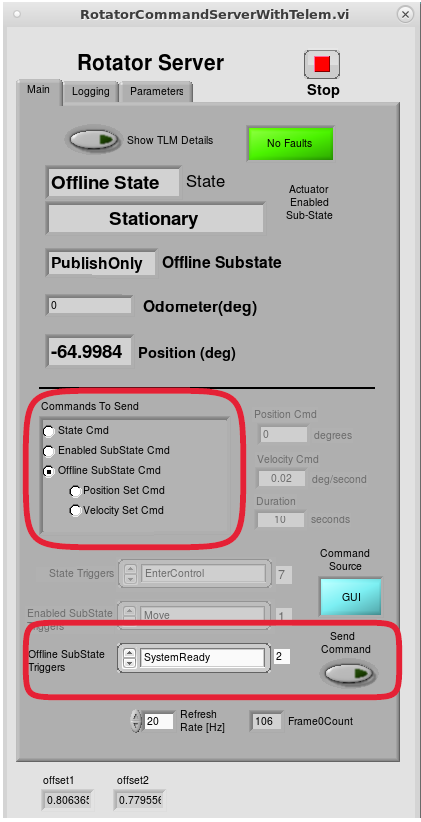
\includegraphics[width=1.79167in]{jira_imgs/1005.png}

}
\hdashrule[0.5ex]{\textwidth}{1pt}{3mm}
  Expected Result \\
{\footnotesize
The system transitions from the OfflineState/PublishOnly substate to the
OfflineState/AvailableState
substate.\\[2\baselineskip]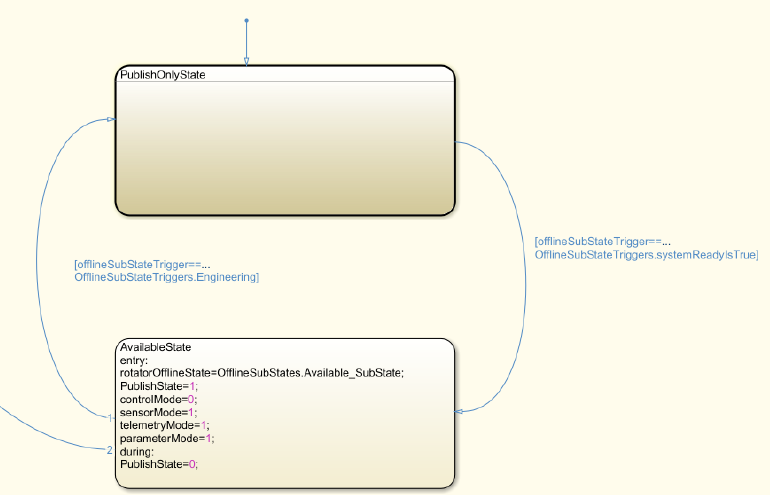
\includegraphics[width=1.79167in]{jira_imgs/1007.png}

}
\hdashrule[0.5ex]{\textwidth}{1pt}{3mm}
  Actual Result \\
{\footnotesize

}
\begin{tabular}{p{2cm}p{14cm}}
\toprule
Step 4 & Step Execution Status: \textbf{ Not Executed } \\ \hline
\end{tabular}
 Description \\
{\footnotesize
\textbf{SWITCHING TO DDS MODE}\\
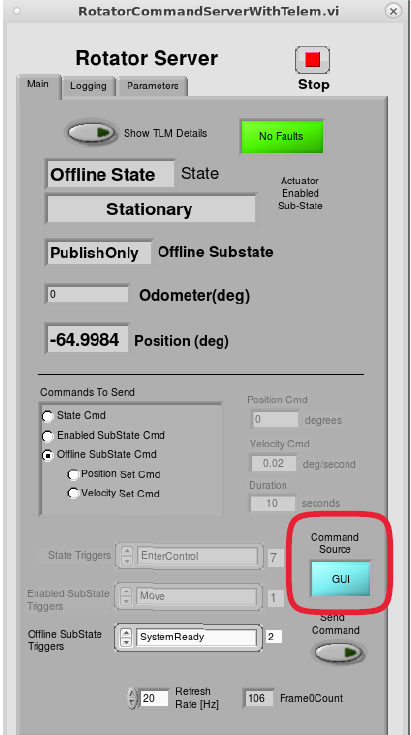
\includegraphics[width=1.79167in]{jira_imgs/1014.png}\\
If the Command Source does not show DDS, go to the Parameters tab,
select DDS under the Command Source and click the Set Command Source
button.\\
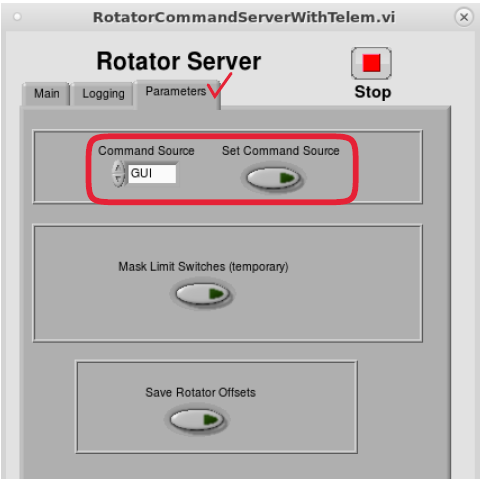
\includegraphics[width=1.79167in]{jira_imgs/1013.png}\textbf{Note:~If
the GUI is used after being set to DDS mode, the system will switch back
the Command Source to GUI and ignore any DDS commands. The Command
Source must show DDS in order to receive DDS commands.}

}
\hdashrule[0.5ex]{\textwidth}{1pt}{3mm}
  Expected Result \\
{\footnotesize
The system is capable of receiving/responding to DDS commands.

}
\hdashrule[0.5ex]{\textwidth}{1pt}{3mm}
  Actual Result \\
{\footnotesize

}
\begin{tabular}{p{2cm}p{14cm}}
\toprule
Step 5 & Step Execution Status: \textbf{ Not Executed } \\ \hline
\end{tabular}
 Description \\
{\footnotesize
\textbf{OFFLINE/PUBLISHONLY -\textgreater{} OFFLINE/SYSTEMREADY}\\
Trigger an interlock fault , send clearError

}
\hdashrule[0.5ex]{\textwidth}{1pt}{3mm}
  Expected Result \\
{\footnotesize
Offline/systemReady

}
\hdashrule[0.5ex]{\textwidth}{1pt}{3mm}
  Actual Result \\
{\footnotesize

}
\begin{tabular}{p{2cm}p{14cm}}
\toprule
Step 6 & Step Execution Status: \textbf{ Not Executed } \\ \hline
\end{tabular}
 Description \\
{\footnotesize
\textbf{OFFLINESTATE -\textgreater{} STANDBYSTATE}\\
The system receives an \emph{enterControl State Transition} command
through DDS.

}
\hdashrule[0.5ex]{\textwidth}{1pt}{3mm}
  Expected Result \\
{\footnotesize
The system transitions into the StandbyState and is capable of
receiving/responding to DDS commands.\\
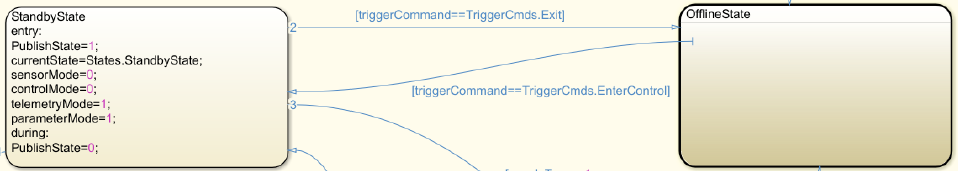
\includegraphics[width=4.68750in]{jira_imgs/1018.png}

}
\hdashrule[0.5ex]{\textwidth}{1pt}{3mm}
  Actual Result \\
{\footnotesize

}
\begin{tabular}{p{2cm}p{14cm}}
\toprule
Step 7 & Step Execution Status: \textbf{ Not Executed } \\ \hline
\end{tabular}
 Description \\
{\footnotesize
\textbf{STANDBYSTATE -\textgreater{} DISABLEDSTATE}\\
From the StandbyState, send a \emph{start} command through the DDS.

}
\hdashrule[0.5ex]{\textwidth}{1pt}{3mm}
  Expected Result \\
{\footnotesize
The system transitions into DisabledState after receiving/responding to
DDS command and the wrapper in the PXI real time controller looks for
the configuration file.\\
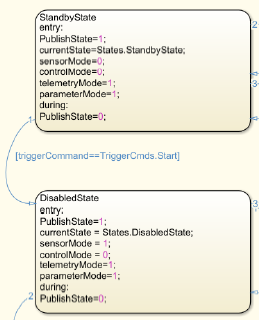
\includegraphics[width=1.79167in]{jira_imgs/1019.png}\\
If the configuration file is invalid or out of range, the system will
transition into a Fault State

}
\hdashrule[0.5ex]{\textwidth}{1pt}{3mm}
  Actual Result \\
{\footnotesize

}
\begin{tabular}{p{2cm}p{14cm}}
\toprule
Step 8 & Step Execution Status: \textbf{ Not Executed } \\ \hline
\end{tabular}
 Description \\
{\footnotesize
\textbf{DISABLEDSTATE -\textgreater{} ENABLEDSTATE}\\
From the DisabledState, send an \emph{enable state} command through the
DDS.

}
\hdashrule[0.5ex]{\textwidth}{1pt}{3mm}
  Expected Result \\
{\footnotesize
The system transitions into the EnabledState/Stationary substate, the
motor drives are enabled, motor brakes are released and the system is
capable of receiving/responding to DDS commands.\\
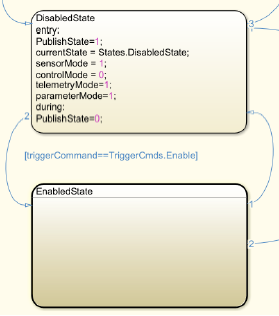
\includegraphics[width=1.79167in]{jira_imgs/1020.png}\\

}
\hdashrule[0.5ex]{\textwidth}{1pt}{3mm}
  Actual Result \\
{\footnotesize

}
\begin{tabular}{p{2cm}p{14cm}}
\toprule
Step 9 & Step Execution Status: \textbf{ Not Executed } \\ \hline
\end{tabular}
 Description \\
{\footnotesize
\textbf{FAULTSTATE}\\
If a Fault occurs in any of the other states, the system will
automatically transition to the Fault State. While in the Fault state,
send a \emph{clearError~}command through the DDS.\\
Note: If the fault that occurs goes through the interlock system, reset
the safety relay switch and send a \emph{clearError~}command.

}
\hdashrule[0.5ex]{\textwidth}{1pt}{3mm}
  Expected Result \\
{\footnotesize
The system transitions back to the Standby state and is not capable of
receiving/responding to DDS commands. (Go back to Step 3) {Include
updated state machine}

}
\hdashrule[0.5ex]{\textwidth}{1pt}{3mm}
  Actual Result \\
{\footnotesize

}
\begin{tabular}{p{2cm}p{14cm}}
\toprule
Step 10 & Step Execution Status: \textbf{ Not Executed } \\ \hline
\end{tabular}
 Description \\
{\footnotesize
\textbf{GUI vs DDS Control}\\[2\baselineskip]While in DDS mode, send a
command from the EUI to test if an EUI user may take over control of the
camera rotator.

}
\hdashrule[0.5ex]{\textwidth}{1pt}{3mm}
  Expected Result \\
{\footnotesize
The system switches from DDS mode to GUI mode. The user must switch back
to the DDS Command Source through the GUI for the system to be
controlled through the CSC again.

}
\hdashrule[0.5ex]{\textwidth}{1pt}{3mm}
  Actual Result \\
{\footnotesize

}
\begin{tabular}{p{2cm}p{14cm}}
\toprule
Step 11 & Step Execution Status: \textbf{ Not Executed } \\ \hline
\end{tabular}
 Description \\
{\footnotesize
\textbf{Back To DDS Mode}\\
While the system is in GUI mode, go to the Parameters tab, select DDS
under the Command Source and click the Set Command Source
button\textbf{.~}

}
\hdashrule[0.5ex]{\textwidth}{1pt}{3mm}
  Expected Result \\
{\footnotesize
The system is capable of receiving/responding to DDS commands.

}
\hdashrule[0.5ex]{\textwidth}{1pt}{3mm}
  Actual Result \\
{\footnotesize

}
\begin{tabular}{p{2cm}p{14cm}}
\toprule
Step 12 & Step Execution Status: \textbf{ Not Executed } \\ \hline
\end{tabular}
 Description \\
{\footnotesize
Use a Jupyter notebook to execute the tests in this test case:\\
Use the latest version available on GitHub for:\\[2\baselineskip]Camera
Rotator Software Re-verification.ipynb

}
\hdashrule[0.5ex]{\textwidth}{1pt}{3mm}
  Expected Result \\
{\footnotesize
The notebook is available\\[2\baselineskip]

}
\hdashrule[0.5ex]{\textwidth}{1pt}{3mm}
  Actual Result \\
{\footnotesize

}
\begin{tabular}{p{2cm}p{14cm}}
\toprule
Step 13 & Step Execution Status: \textbf{ Not Executed } \\ \hline
\end{tabular}
 Description \\
{\footnotesize
\textbf{Test Sequence \#1 -- Move Commands}\\[2\baselineskip]Record the
current position of the Rotator.

}
\hdashrule[0.5ex]{\textwidth}{1pt}{3mm}
  Test Data \\
 {\footnotesize
\textbf{Note:~}When executing this test, write out the timestamp for the
start and end of this test sequence in the Actual Results field so that
this can easily be found in the EFD.

}
\hdashrule[0.5ex]{\textwidth}{1pt}{3mm}
  Expected Result \\
{\footnotesize
The initial position of the Camera Rotator is recorded.

}
\hdashrule[0.5ex]{\textwidth}{1pt}{3mm}
  Actual Result \\
{\footnotesize

}
\begin{tabular}{p{2cm}p{14cm}}
\toprule
Step 14 & Step Execution Status: \textbf{ Not Executed } \\ \hline
\end{tabular}
 Description \\
{\footnotesize
In the Enabled/Stationary state, send a \emph{move} command to position
the Rotator at 15deg.\\[2\baselineskip]

}
\hdashrule[0.5ex]{\textwidth}{1pt}{3mm}
  Expected Result \\
{\footnotesize
Confirm that the rotator moves to 15deg and an \emph{inPosition} event
is generated when the move is complete.

}
\hdashrule[0.5ex]{\textwidth}{1pt}{3mm}
  Actual Result \\
{\footnotesize

}
\begin{tabular}{p{2cm}p{14cm}}
\toprule
Step 15 & Step Execution Status: \textbf{ Not Executed } \\ \hline
\end{tabular}
 Description \\
{\footnotesize
Record the corresponding DDS events that were generated.

}
\hdashrule[0.5ex]{\textwidth}{1pt}{3mm}
  Expected Result \\
{\footnotesize
\begin{itemize}
\tightlist
\item
  The \emph{Application} event outputs reasonable values
\item
  The controllerState.enabledSubstate goes to MOVING\_POINT\_TO\_POINT
  when the move begins and STATIONARY when the move ends
\end{itemize}

}
\hdashrule[0.5ex]{\textwidth}{1pt}{3mm}
  Actual Result \\
{\footnotesize

}
\begin{tabular}{p{2cm}p{14cm}}
\toprule
Step 16 & Step Execution Status: \textbf{ Not Executed } \\ \hline
\end{tabular}
 Description \\
{\footnotesize
\textbf{Section 3.2.2 of the attached Software Acceptance Test
Procedure\\
Test Sequence \#2 - Stop Command}\\[2\baselineskip]In the
enabled/Stationary state, send a move command to 50deg.

}
\hdashrule[0.5ex]{\textwidth}{1pt}{3mm}
  Test Data \\
 {\footnotesize
\textbf{Note:~}When executing this test, write out the timestamp for the
start and end of this test sequence in the Actual Results field so that
this can easily be found in the EFD.

}
\hdashrule[0.5ex]{\textwidth}{1pt}{3mm}
  Expected Result \\
{\footnotesize
Confirm that the rotator starts to move to +50deg.

}
\hdashrule[0.5ex]{\textwidth}{1pt}{3mm}
  Actual Result \\
{\footnotesize

}
\begin{tabular}{p{2cm}p{14cm}}
\toprule
Step 17 & Step Execution Status: \textbf{ Not Executed } \\ \hline
\end{tabular}
 Description \\
{\footnotesize
While the rotator is still moving, send a \emph{stop} command.

}
\hdashrule[0.5ex]{\textwidth}{1pt}{3mm}
  Expected Result \\
{\footnotesize
Confirm that the system quickly comes to a stop before reaching the 50
deg position.

}
\hdashrule[0.5ex]{\textwidth}{1pt}{3mm}
  Actual Result \\
{\footnotesize

}
\begin{tabular}{p{2cm}p{14cm}}
\toprule
Step 18 & Step Execution Status: \textbf{ Not Executed } \\ \hline
\end{tabular}
 Description \\
{\footnotesize
Record the current position and then send a move command to -60deg.

}
\hdashrule[0.5ex]{\textwidth}{1pt}{3mm}
  Expected Result \\
{\footnotesize
Confirm the rotator moves to the commanded position (-60deg) following
the previous \emph{stop} command.

}
\hdashrule[0.5ex]{\textwidth}{1pt}{3mm}
  Actual Result \\
{\footnotesize

}
\begin{tabular}{p{2cm}p{14cm}}
\toprule
Step 19 & Step Execution Status: \textbf{ Not Executed } \\ \hline
\end{tabular}
 Description \\
{\footnotesize
Wait 39s.

}
\hdashrule[0.5ex]{\textwidth}{1pt}{3mm}
  Expected Result \\
{\footnotesize

}
\hdashrule[0.5ex]{\textwidth}{1pt}{3mm}
  Actual Result \\
{\footnotesize

}
\begin{tabular}{p{2cm}p{14cm}}
\toprule
Step 20 & Step Execution Status: \textbf{ Not Executed } \\ \hline
\end{tabular}
 Description \\
{\footnotesize
Record the corresponding DDS events that were generated.

}
\hdashrule[0.5ex]{\textwidth}{1pt}{3mm}
  Expected Result \\
{\footnotesize
\begin{itemize}
\tightlist
\item
  The controllerState.enabledSubstate goes to CONTROLLED\_STOPPING when
  the stop is requested, then STATIONARY when the rotator has halted
\item
  The \emph{inPosition} event is not reported as True.
\end{itemize}

}
\hdashrule[0.5ex]{\textwidth}{1pt}{3mm}
  Actual Result \\
{\footnotesize

}
\begin{tabular}{p{2cm}p{14cm}}
\toprule
Step 21 & Step Execution Status: \textbf{ Not Executed } \\ \hline
\end{tabular}
 Description \\
{\footnotesize
\textbf{Test of trackStart and track command}\\[2\baselineskip]In the
Enabled state, send a \emph{trackStart} command. Do not send a
\emph{Track} command.

}
\hdashrule[0.5ex]{\textwidth}{1pt}{3mm}
  Expected Result \\
{\footnotesize
The cRIO goes into FAULT state without moving at all.

}
\hdashrule[0.5ex]{\textwidth}{1pt}{3mm}
  Actual Result \\
{\footnotesize

}
\begin{tabular}{p{2cm}p{14cm}}
\toprule
Step 22 & Step Execution Status: \textbf{ Not Executed } \\ \hline
\end{tabular}
 Description \\
{\footnotesize
\textbf{Section 3.2.2 of the attached Software Acceptance Test
Procedure\\
Test Sequence \#4 - Track and TrackStart Commands}\\[2\baselineskip]In
the Enabled/Stationary state, send a \emph{trackStart} command.

}
\hdashrule[0.5ex]{\textwidth}{1pt}{3mm}
  Expected Result \\
{\footnotesize
Confirm that the system transitions into Enabled/Slewing and Tracking
state.

}
\hdashrule[0.5ex]{\textwidth}{1pt}{3mm}
  Actual Result \\
{\footnotesize

}
\begin{tabular}{p{2cm}p{14cm}}
\toprule
Step 23 & Step Execution Status: \textbf{ Not Executed } \\ \hline
\end{tabular}
 Description \\
{\footnotesize
Send a series of \emph{track} commands at 20 Hz from
command\_vector\_set\_A.mat and ensure the system follows the commands
and sends appropriate tracking and trackLost events.

}
\hdashrule[0.5ex]{\textwidth}{1pt}{3mm}
  Test Data \\
 {\footnotesize
\textbf{Deviation:} When the \emph{trackStart} command is run, a track
command must be issued at 10-20Hz until tracking is done. The vendor's
code reads in a CSV file with tracking conditions when using the
\emph{trackStart} command in order to circumvent a FAULT state due to
lack of position, velocity and time updates. Instead, use Russell's code
which utilizes the functions \emph{ramp~}and\emph{~sine~}to track from a
start position to an end position at a specified velocity and track
along a sine wave, respectively.

}
\hdashrule[0.5ex]{\textwidth}{1pt}{3mm}
  Expected Result \\
{\footnotesize
The rotator first slews to meet the commanded path and then tracks that
path

}
\hdashrule[0.5ex]{\textwidth}{1pt}{3mm}
  Actual Result \\
{\footnotesize

}
\begin{tabular}{p{2cm}p{14cm}}
\toprule
Step 24 & Step Execution Status: \textbf{ Not Executed } \\ \hline
\end{tabular}
 Description \\
{\footnotesize
Record the corresponding DDS events that were generated.

}
\hdashrule[0.5ex]{\textwidth}{1pt}{3mm}
  Expected Result \\
{\footnotesize
\begin{itemize}
\tightlist
\item
  The \emph{Application~}event outputs reasonable values
\item
  The controllerState.enabledSubstate goes to SLEWING\_OR\_TRACKING when
  the move begins, CONTROLLED\_STOPPING when the movement sequence ends,
  and STATIONARY when the rotator has stopped
\item
  The \emph{inPosition} event is True once slewing has finished and
  tracking begins
\end{itemize}

}
\hdashrule[0.5ex]{\textwidth}{1pt}{3mm}
  Actual Result \\
{\footnotesize

}
\begin{tabular}{p{2cm}p{14cm}}
\toprule
Step 25 & Step Execution Status: \textbf{ Not Executed } \\ \hline
\end{tabular}
 Description \\
{\footnotesize
\textbf{Section 3.2.2 of the attached Software Acceptance Test
Procedure\\
Test Sequence \#5 - Track and TrackStart Commands}\\[2\baselineskip]In
the Enabled/Stationary state, send a \emph{trackStart} command.

}
\hdashrule[0.5ex]{\textwidth}{1pt}{3mm}
  Expected Result \\
{\footnotesize
Confirm that the system transitions into Enabled/Slewing and Tracking
state.

}
\hdashrule[0.5ex]{\textwidth}{1pt}{3mm}
  Actual Result \\
{\footnotesize

}
\begin{tabular}{p{2cm}p{14cm}}
\toprule
Step 26 & Step Execution Status: \textbf{ Not Executed } \\ \hline
\end{tabular}
 Description \\
{\footnotesize
Send a series of \emph{track} commands at 20 Hz from
command\_vector\_set\_B.mat and ensure the system follows the commands
and sends appropriate tracking and trackLost events.

}
\hdashrule[0.5ex]{\textwidth}{1pt}{3mm}
  Test Data \\
 {\footnotesize
\textbf{Deviation:} When the \emph{trackStart} command is run, a track
command must be issued at 10-20Hz until tracking is done. The vendor's
code reads in a CSV file with tracking conditions when using the
\emph{trackStart} command in order to circumvent a FAULT state due to
lack of position, velocity and time updates. Instead, use Russell's code
which utilizes the functions \emph{ramp~}and\emph{~sine~}to track from a
start position to an end position at a specified velocity and track
along a sine wave, respectively.

}
\hdashrule[0.5ex]{\textwidth}{1pt}{3mm}
  Expected Result \\
{\footnotesize
The rotator first slews to meet the commanded path and then tracks that
path

}
\hdashrule[0.5ex]{\textwidth}{1pt}{3mm}
  Actual Result \\
{\footnotesize

}
\begin{tabular}{p{2cm}p{14cm}}
\toprule
Step 27 & Step Execution Status: \textbf{ Not Executed } \\ \hline
\end{tabular}
 Description \\
{\footnotesize
Record the corresponding DDS events that were generated.

}
\hdashrule[0.5ex]{\textwidth}{1pt}{3mm}
  Expected Result \\
{\footnotesize
\begin{itemize}
\tightlist
\item
  The \emph{Application~}event outputs reasonable values
\item
  The controllerState.enabledSubstate goes to SLEWING\_OR\_TRACKING when
  the move begins, CONTROLLED\_STOPPING when the movement sequence ends,
  and STATIONARY when the rotator has stopped
\item
  The \emph{inPosition} event is True once slewing has finished and
  tracking begins
\end{itemize}

}
\hdashrule[0.5ex]{\textwidth}{1pt}{3mm}
  Actual Result \\
{\footnotesize

}
\begin{tabular}{p{2cm}p{14cm}}
\toprule
Step 28 & Step Execution Status: \textbf{ Not Executed } \\ \hline
\end{tabular}
 Description \\
{\footnotesize
\textbf{Section 3.2.2 of the attached Software Acceptance Test
Procedure\\
Test Sequence \#6 - configureVelocity Command}\\[2\baselineskip]In the
Enabled/Stationary state, send a \emph{configureVelocity} command of 4
deg/s.

}
\hdashrule[0.5ex]{\textwidth}{1pt}{3mm}
  Expected Result \\
{\footnotesize
Confirm that the command is rejected for being out of acceptable range.

}
\hdashrule[0.5ex]{\textwidth}{1pt}{3mm}
  Actual Result \\
{\footnotesize

}
\begin{tabular}{p{2cm}p{14cm}}
\toprule
Step 29 & Step Execution Status: \textbf{ Not Executed } \\ \hline
\end{tabular}
 Description \\
{\footnotesize
Send a \emph{configureVelocity} command of 0.5 deg/s.

}
\hdashrule[0.5ex]{\textwidth}{1pt}{3mm}
  Expected Result \\
{\footnotesize
Confirm that this command is accepted.

}
\hdashrule[0.5ex]{\textwidth}{1pt}{3mm}
  Actual Result \\
{\footnotesize

}
\begin{tabular}{p{2cm}p{14cm}}
\toprule
Step 30 & Step Execution Status: \textbf{ Not Executed } \\ \hline
\end{tabular}
 Description \\
{\footnotesize
Record the current position and send a \emph{move~}command to a position
10 deg away from the current position.

}
\hdashrule[0.5ex]{\textwidth}{1pt}{3mm}
  Expected Result \\
{\footnotesize
Confirm the that move in completed in approximately 20 seconds.

}
\hdashrule[0.5ex]{\textwidth}{1pt}{3mm}
  Actual Result \\
{\footnotesize

}
\begin{tabular}{p{2cm}p{14cm}}
\toprule
Step 31 & Step Execution Status: \textbf{ Not Executed } \\ \hline
\end{tabular}
 Description \\
{\footnotesize
Record the corresponding DDS events that were generated.

}
\hdashrule[0.5ex]{\textwidth}{1pt}{3mm}
  Expected Result \\
{\footnotesize
\begin{itemize}
\tightlist
\item
  The \emph{Application} event outputs reasonable values
\item
  The controllerState.enabledSubstate goes to MOVING\_POINT\_TO\_POINT
  when the move begins and STATIONARY when the move ends
\item
  The \emph{inPosition} event is True once move has finished
\end{itemize}

}
\hdashrule[0.5ex]{\textwidth}{1pt}{3mm}
  Actual Result \\
{\footnotesize

}
\begin{tabular}{p{2cm}p{14cm}}
\toprule
Step 32 & Step Execution Status: \textbf{ Not Executed } \\ \hline
\end{tabular}
 Description \\
{\footnotesize
\textbf{Section 3.2.2 of the attached Software Acceptance Test
Procedure\\
Test Sequence \#7 - configureAcceleration Command}\\[2\baselineskip]In
the Enabled/Stationary state with the \emph{configureVelocity} command
from the previous test still in effect, send a
\emph{configureAcceleration} command of 2 deg/s\^{}2.

}
\hdashrule[0.5ex]{\textwidth}{1pt}{3mm}
  Expected Result \\
{\footnotesize
Confirm that the command is rejected for being out of acceptable range.

}
\hdashrule[0.5ex]{\textwidth}{1pt}{3mm}
  Actual Result \\
{\footnotesize

}
\begin{tabular}{p{2cm}p{14cm}}
\toprule
Step 33 & Step Execution Status: \textbf{ Not Executed } \\ \hline
\end{tabular}
 Description \\
{\footnotesize
Send a \emph{configureAcceleration} command of 0.05 deg/s\^{}2.

}
\hdashrule[0.5ex]{\textwidth}{1pt}{3mm}
  Expected Result \\
{\footnotesize
Confirm that the command is accepted.

}
\hdashrule[0.5ex]{\textwidth}{1pt}{3mm}
  Actual Result \\
{\footnotesize

}
\begin{tabular}{p{2cm}p{14cm}}
\toprule
Step 34 & Step Execution Status: \textbf{ Not Executed } \\ \hline
\end{tabular}
 Description \\
{\footnotesize
Record the current position and send a move\emph{~}command to a position
10 deg away from the current position.

}
\hdashrule[0.5ex]{\textwidth}{1pt}{3mm}
  Expected Result \\
{\footnotesize
Confirm the that move in completed in approximately 30 seconds.

}
\hdashrule[0.5ex]{\textwidth}{1pt}{3mm}
  Actual Result \\
{\footnotesize

}
\begin{tabular}{p{2cm}p{14cm}}
\toprule
Step 35 & Step Execution Status: \textbf{ Not Executed } \\ \hline
\end{tabular}
 Description \\
{\footnotesize
Record the corresponding DDS events that were generated.

}
\hdashrule[0.5ex]{\textwidth}{1pt}{3mm}
  Expected Result \\
{\footnotesize
\begin{itemize}
\tightlist
\item
  The \emph{Application} event outputs reasonable values
\item
  The controllerState.enabledSubstate goes to MOVING\_POINT\_TO\_POINT
  when the move begins and STATIONARY when the move ends
\item
  The \emph{inPosition} event is True once move has finished
\end{itemize}

}
\hdashrule[0.5ex]{\textwidth}{1pt}{3mm}
  Actual Result \\
{\footnotesize

}
\begin{tabular}{p{2cm}p{14cm}}
\toprule
Step 36 & Step Execution Status: \textbf{ Not Executed } \\ \hline
\end{tabular}
 Description \\
{\footnotesize
Shutdown the rotator.

}
\hdashrule[0.5ex]{\textwidth}{1pt}{3mm}
  Expected Result \\
{\footnotesize
Rotator is shutdown.

}
\hdashrule[0.5ex]{\textwidth}{1pt}{3mm}
  Actual Result \\
{\footnotesize

}
\begin{tabular}{p{2cm}p{14cm}}
\toprule
Step 37 & Step Execution Status: \textbf{ Not Executed } \\ \hline
\end{tabular}
 Description \\
{\footnotesize
\textbf{Section 3.3.2 of the attached Software Acceptance Test
Procedure}\\
\textbf{Rotator Action on State Commands\\
}\\
Start up the system.

}
\hdashrule[0.5ex]{\textwidth}{1pt}{3mm}
  Expected Result \\
{\footnotesize
\begin{itemize}
\tightlist
\item
  Confirm the system starts up in Offline/PublishOnly state.
\item
  When the middleware starts up, confirm that a \emph{SettingsVersions}
  event is published with a list of all saved settings file names and a
  \emph{settingsApplied} event is published with a list of all default
  configurable parameters.
\end{itemize}

}
\hdashrule[0.5ex]{\textwidth}{1pt}{3mm}
  Actual Result \\
{\footnotesize

}
\begin{tabular}{p{2cm}p{14cm}}
\toprule
Step 38 & Step Execution Status: \textbf{ Not Executed } \\ \hline
\end{tabular}
 Description \\
{\footnotesize
Send the \emph{enterControl} command.

}
\hdashrule[0.5ex]{\textwidth}{1pt}{3mm}
  Expected Result \\
{\footnotesize
Confirm that the system does not respond to a \emph{EnterControl}
command over DDS.

}
\hdashrule[0.5ex]{\textwidth}{1pt}{3mm}
  Actual Result \\
{\footnotesize

}
\begin{tabular}{p{2cm}p{14cm}}
\toprule
Step 39 & Step Execution Status: \textbf{ Not Executed } \\ \hline
\end{tabular}
 Description \\
{\footnotesize
From the EUI send an offline substate trigger of \emph{systemReady}.

}
\hdashrule[0.5ex]{\textwidth}{1pt}{3mm}
  Expected Result \\
{\footnotesize
Confirm system goes into Offline/Available substate.

}
\hdashrule[0.5ex]{\textwidth}{1pt}{3mm}
  Actual Result \\
{\footnotesize

}
\begin{tabular}{p{2cm}p{14cm}}
\toprule
Step 40 & Step Execution Status: \textbf{ Not Executed } \\ \hline
\end{tabular}
 Description \\
{\footnotesize
From the EUI, select the DDS button to allow the system to receive
commands from DDS.

}
\hdashrule[0.5ex]{\textwidth}{1pt}{3mm}
  Expected Result \\
{\footnotesize
The EUI displays you are in DDS command mode.

}
\hdashrule[0.5ex]{\textwidth}{1pt}{3mm}
  Actual Result \\
{\footnotesize

}
\begin{tabular}{p{2cm}p{14cm}}
\toprule
Step 41 & Step Execution Status: \textbf{ Not Executed } \\ \hline
\end{tabular}
 Description \\
{\footnotesize
Send an \emph{EnterControl} trigger. Record the corresponding DDS
event(s) that were generated.

}
\hdashrule[0.5ex]{\textwidth}{1pt}{3mm}
  Expected Result \\
{\footnotesize
Confirm the system transitions from Offline/Available to Standby state.

}
\hdashrule[0.5ex]{\textwidth}{1pt}{3mm}
  Actual Result \\
{\footnotesize

}
\begin{tabular}{p{2cm}p{14cm}}
\toprule
Step 42 & Step Execution Status: \textbf{ Not Executed } \\ \hline
\end{tabular}
 Description \\
{\footnotesize
Send a \emph{Start} trigger with an invalid filename.

}
\hdashrule[0.5ex]{\textwidth}{1pt}{3mm}
  Expected Result \\
{\footnotesize
Verify that the command is rejected and the system does not transition
out of Standby state.

}
\hdashrule[0.5ex]{\textwidth}{1pt}{3mm}
  Actual Result \\
{\footnotesize

}
\begin{tabular}{p{2cm}p{14cm}}
\toprule
Step 43 & Step Execution Status: \textbf{ Not Executed } \\ \hline
\end{tabular}
 Description \\
{\footnotesize
Send a \emph{Start} trigger with a valid filename. Record the
corresponding DDS event(s) that were generated.

}
\hdashrule[0.5ex]{\textwidth}{1pt}{3mm}
  Expected Result \\
{\footnotesize
Confirm the system transitions from Standby to Disabled state and a
\emph{settingApplied} and \emph{AppliedSettingsMatchStart} = True events
are generated.

}
\hdashrule[0.5ex]{\textwidth}{1pt}{3mm}
  Actual Result \\
{\footnotesize

}
\begin{tabular}{p{2cm}p{14cm}}
\toprule
Step 44 & Step Execution Status: \textbf{ Not Executed } \\ \hline
\end{tabular}
 Description \\
{\footnotesize
Send an \emph{Enable} trigger. Record the corresponding DDS event(s)
that were generated.

}
\hdashrule[0.5ex]{\textwidth}{1pt}{3mm}
  Expected Result \\
{\footnotesize
Confirm the system transitions from Disabled to Enabled state.

}
\hdashrule[0.5ex]{\textwidth}{1pt}{3mm}
  Actual Result \\
{\footnotesize

}
\begin{tabular}{p{2cm}p{14cm}}
\toprule
Step 45 & Step Execution Status: \textbf{ Not Executed } \\ \hline
\end{tabular}
 Description \\
{\footnotesize
Send a \emph{Disable} trigger. Record the corresponding DDS event(s)
that were generated.

}
\hdashrule[0.5ex]{\textwidth}{1pt}{3mm}
  Expected Result \\
{\footnotesize
Confirm the system transitions from Enabled to Disabled state.

}
\hdashrule[0.5ex]{\textwidth}{1pt}{3mm}
  Actual Result \\
{\footnotesize

}
\begin{tabular}{p{2cm}p{14cm}}
\toprule
Step 46 & Step Execution Status: \textbf{ Not Executed } \\ \hline
\end{tabular}
 Description \\
{\footnotesize
Send a \emph{Standby} trigger. Record the corresponding DDS event(s)
that were generated.

}
\hdashrule[0.5ex]{\textwidth}{1pt}{3mm}
  Expected Result \\
{\footnotesize
Confirm the system transitions from Disabled state to Standby state.

}
\hdashrule[0.5ex]{\textwidth}{1pt}{3mm}
  Actual Result \\
{\footnotesize

}
\begin{tabular}{p{2cm}p{14cm}}
\toprule
Step 47 & Step Execution Status: \textbf{ Not Executed } \\ \hline
\end{tabular}
 Description \\
{\footnotesize
Send a \emph{exitControl} trigger. Record the corresponding DDS event(s)
that were generated.

}
\hdashrule[0.5ex]{\textwidth}{1pt}{3mm}
  Expected Result \\
{\footnotesize
Confirm the system transitions from Standby state to Offline state.

}
\hdashrule[0.5ex]{\textwidth}{1pt}{3mm}
  Actual Result \\
{\footnotesize

}
\begin{tabular}{p{2cm}p{14cm}}
\toprule
Step 48 & Step Execution Status: \textbf{ Not Executed } \\ \hline
\end{tabular}
 Description \\
{\footnotesize
\textbf{Section 5.1 of the attached Software Acceptance Test
Procedure}\\
\textbf{Rotator Events\\
}\\
In the Enabled state, unplug an encoder cable for one of the rotator
motors.

}
\hdashrule[0.5ex]{\textwidth}{1pt}{3mm}
  Test Data \\
 {\footnotesize
\textbf{NOTE:} After each step in this set of steps, we will need to
send the clearError command to the CSC. This will put the cRIO into
Offline/PublishOnly. Use the EUI to re-enable CSC control.

}
\hdashrule[0.5ex]{\textwidth}{1pt}{3mm}
  Expected Result \\
{\footnotesize
Confirm that a \emph{Drive Fault} event is created and the system
transitions to Fault state.

}
\hdashrule[0.5ex]{\textwidth}{1pt}{3mm}
  Actual Result \\
{\footnotesize

}
\begin{tabular}{p{2cm}p{14cm}}
\toprule
Step 49 & Step Execution Status: \textbf{ Not Executed } \\ \hline
\end{tabular}
 Description \\
{\footnotesize
In the Enabled state, unplug a linear encoder cable for the rotator.

}
\hdashrule[0.5ex]{\textwidth}{1pt}{3mm}
  Expected Result \\
{\footnotesize
Confirm that a \emph{Linear Encoder Error} event is created and the
system transitions to Fault state.

}
\hdashrule[0.5ex]{\textwidth}{1pt}{3mm}
  Actual Result \\
{\footnotesize

}
\begin{tabular}{p{2cm}p{14cm}}
\toprule
Step 50 & Step Execution Status: \textbf{ Not Executed } \\ \hline
\end{tabular}
 Description \\
{\footnotesize
Set the Following Error Threshold parameter to a very small value
(0.0001 deg or smaller).

}
\hdashrule[0.5ex]{\textwidth}{1pt}{3mm}
  Test Data \\
 {\footnotesize
Adjust this value within the configuration file of the PXI and reboot
the software.~

}
\hdashrule[0.5ex]{\textwidth}{1pt}{3mm}
  Expected Result \\
{\footnotesize

}
\hdashrule[0.5ex]{\textwidth}{1pt}{3mm}
  Actual Result \\
{\footnotesize

}
\begin{tabular}{p{2cm}p{14cm}}
\toprule
Step 51 & Step Execution Status: \textbf{ Not Executed } \\ \hline
\end{tabular}
 Description \\
{\footnotesize
Send a \emph{move} command.

}
\hdashrule[0.5ex]{\textwidth}{1pt}{3mm}
  Expected Result \\
{\footnotesize
Confirm that a \emph{Following Error} event is created and the system
transitions to Fault state.

}
\hdashrule[0.5ex]{\textwidth}{1pt}{3mm}
  Actual Result \\
{\footnotesize

}
\begin{tabular}{p{2cm}p{14cm}}
\toprule
Step 52 & Step Execution Status: \textbf{ Not Executed } \\ \hline
\end{tabular}
 Description \\
{\footnotesize
Activate the positive software limit using a special control program.

}
\hdashrule[0.5ex]{\textwidth}{1pt}{3mm}
  Expected Result \\
{\footnotesize
Confirm that a \emph{Positive Limit Switch} error message is created and
the system transitions to Fault state.

}
\hdashrule[0.5ex]{\textwidth}{1pt}{3mm}
  Actual Result \\
{\footnotesize

}
\begin{tabular}{p{2cm}p{14cm}}
\toprule
Step 53 & Step Execution Status: \textbf{ Not Executed } \\ \hline
\end{tabular}
 Description \\
{\footnotesize
Activate the negative software limit using a special control program.

}
\hdashrule[0.5ex]{\textwidth}{1pt}{3mm}
  Expected Result \\
{\footnotesize
Confirm that a \emph{Negative Limit Switch} error message is created and
the system transitions to Fault State.

}
\hdashrule[0.5ex]{\textwidth}{1pt}{3mm}
  Actual Result \\
{\footnotesize

}
\begin{tabular}{p{2cm}p{14cm}}
\toprule
Step 54 & Step Execution Status: \textbf{ Not Executed } \\ \hline
\end{tabular}
 Description \\
{\footnotesize
Unplug the Ethercat cable between the control PC and the Copley XE2
drive.

}
\hdashrule[0.5ex]{\textwidth}{1pt}{3mm}
  Expected Result \\
{\footnotesize
Confirm that an \emph{Ethercat Problem} event is created and the system
transitions to Fault state.

}
\hdashrule[0.5ex]{\textwidth}{1pt}{3mm}
  Actual Result \\
{\footnotesize

}
\begin{tabular}{p{2cm}p{14cm}}
\toprule
Step 55 & Step Execution Status: \textbf{ Not Executed } \\ \hline
\end{tabular}
 Description \\
{\footnotesize
Shutdown the rotator.

}
\hdashrule[0.5ex]{\textwidth}{1pt}{3mm}
  Expected Result \\
{\footnotesize
Rotator is shutdown.

}
\hdashrule[0.5ex]{\textwidth}{1pt}{3mm}
  Actual Result \\
{\footnotesize

}

\paragraph{ LVV-T2222 - MTAOS Interface to SAL }\mbox{}\\

Version \textbf{1}.
Open  \href{https://jira.lsstcorp.org/secure/Tests.jspa#/testCase/LVV-T2222}{\textit{ LVV-T2222 } }
test case in Jira.

The objective of this test case is to verify the MTAOS communication
interface with SAL by checking the commands as defined in the latest
XML.\\
This test will not verify the functionality of the commands, but will
simply test that the MTAOS is able to publish the commands to SAL.\\
The MTAOS commands, as well as the events, will be fully verified in
later test cycles of the Level 3 Integration Test Plan when the MTAOS is
integrated with the M1M3, M2, and the hexapods.

\textbf{ Preconditions}:\\
\begin{itemize}
\tightlist
\item
  Only requires the MTAOS to be operable~
\item
  Requires the use of SAL/DDS and the EFD
\item
  Does not require any communication with the M1M3, M2, and the hexapods
\end{itemize}

Execution status: {\bf Not Executed }

Final comment:\\


Detailed steps results:

\begin{tabular}{p{2cm}p{14cm}}
\toprule
Step 1 & Step Execution Status: \textbf{ Not Executed } \\ \hline
\end{tabular}
 Description \\
{\footnotesize
The following steps will be expected to be executed using a Jupyter
notebook to send the commands.~

}
\hdashrule[0.5ex]{\textwidth}{1pt}{3mm}
  Expected Result \\
{\footnotesize
The notebook is available.

}
\hdashrule[0.5ex]{\textwidth}{1pt}{3mm}
  Actual Result \\
{\footnotesize

}
\begin{tabular}{p{2cm}p{14cm}}
\toprule
Step 2 & Step Execution Status: \textbf{ Not Executed } \\ \hline
\end{tabular}
 Description \\
{\footnotesize
Send an~\emph{MTAOS\_command\_preProcess} command through SAL.

}
\hdashrule[0.5ex]{\textwidth}{1pt}{3mm}
  Expected Result \\
{\footnotesize
The command is published to the EFD.

}
\hdashrule[0.5ex]{\textwidth}{1pt}{3mm}
  Actual Result \\
{\footnotesize

}
\begin{tabular}{p{2cm}p{14cm}}
\toprule
Step 3 & Step Execution Status: \textbf{ Not Executed } \\ \hline
\end{tabular}
 Description \\
{\footnotesize
Send ~\emph{MTAOS\_command\_runWEP} command to start the Wavefront
Estimation Pipeline (WEP) through SAL.

}
\hdashrule[0.5ex]{\textwidth}{1pt}{3mm}
  Expected Result \\
{\footnotesize
The command is accepted and the \emph{MTAOS\_logevent\_wepDuration} is
published to the EFD at its completion.~

}
\hdashrule[0.5ex]{\textwidth}{1pt}{3mm}
  Actual Result \\
{\footnotesize

}
\begin{tabular}{p{2cm}p{14cm}}
\toprule
Step 4 & Step Execution Status: \textbf{ Not Executed } \\ \hline
\end{tabular}
 Description \\
{\footnotesize
Having already sent an \emph{MTAOS\_command\_runWEP~}command, send an
\emph{MTAOS\_command\_runOFC} command to start the Optical Feedback
Controller (OFC).

}
\hdashrule[0.5ex]{\textwidth}{1pt}{3mm}
  Expected Result \\
{\footnotesize
The command is accepted and \emph{MTAOS\_logevent\_ofcDuration} event is
published once the corrections have been computed.~

}
\hdashrule[0.5ex]{\textwidth}{1pt}{3mm}
  Actual Result \\
{\footnotesize

}
\begin{tabular}{p{2cm}p{14cm}}
\toprule
Step 5 & Step Execution Status: \textbf{ Not Executed } \\ \hline
\end{tabular}
 Description \\
{\footnotesize
Send an \emph{MTAOS\_command\_issueCorrection} command through SAL.

}
\hdashrule[0.5ex]{\textwidth}{1pt}{3mm}
  Expected Result \\
{\footnotesize
The corrections based on the results of
the~\emph{MTAOS\_command\_runOFC~}command and the following events are
published:

\begin{itemize}
\tightlist
\item
  \emph{MTAOS\_logevent\_wavefrontError}
\item
  \emph{MTAOS\_logevent\_m2HexapodCorrection}
\item
  \emph{MTAOS\_logevent\_cameraHexapodCorrection}
\item
  \emph{MTAOS\_logevent\_m1m3HexapodCorrection}
\item
  \emph{MTAOS\_logevent\_m2Correction}
\item
  \emph{MTAOS\_logevent\_degreeOfFreedom}
\end{itemize}

}
\hdashrule[0.5ex]{\textwidth}{1pt}{3mm}
  Actual Result \\
{\footnotesize

}
\begin{tabular}{p{2cm}p{14cm}}
\toprule
Step 6 & Step Execution Status: \textbf{ Not Executed } \\ \hline
\end{tabular}
 Description \\
{\footnotesize
Send an~\emph{MTAOS\_command\_addAberration} command through SAL.

}
\hdashrule[0.5ex]{\textwidth}{1pt}{3mm}
  Expected Result \\
{\footnotesize
The command is published to the EFD with the parameters for wfX and
config filled with reasonable values.

}
\hdashrule[0.5ex]{\textwidth}{1pt}{3mm}
  Actual Result \\
{\footnotesize

}
\begin{tabular}{p{2cm}p{14cm}}
\toprule
Step 7 & Step Execution Status: \textbf{ Not Executed } \\ \hline
\end{tabular}
 Description \\
{\footnotesize
Send an \emph{MTAOS\_command\_resetCorrection~}command through SAL.

}
\hdashrule[0.5ex]{\textwidth}{1pt}{3mm}
  Expected Result \\
{\footnotesize
The command is published to the EFD and all the corrections that were
previously issued are reset.

}
\hdashrule[0.5ex]{\textwidth}{1pt}{3mm}
  Actual Result \\
{\footnotesize

}
\begin{tabular}{p{2cm}p{14cm}}
\toprule
Step 8 & Step Execution Status: \textbf{ Not Executed } \\ \hline
\end{tabular}
 Description \\
{\footnotesize
Send another \emph{MTAOS\_command\_runWEP} command.

}
\hdashrule[0.5ex]{\textwidth}{1pt}{3mm}
  Expected Result \\
{\footnotesize
The command is accepted.

}
\hdashrule[0.5ex]{\textwidth}{1pt}{3mm}
  Actual Result \\
{\footnotesize

}
\begin{tabular}{p{2cm}p{14cm}}
\toprule
Step 9 & Step Execution Status: \textbf{ Not Executed } \\ \hline
\end{tabular}
 Description \\
{\footnotesize
Having already sent an \emph{MTAOS\_command\_runWEP~}command, send an
\emph{MTAOS\_command\_runOFC} command.

}
\hdashrule[0.5ex]{\textwidth}{1pt}{3mm}
  Expected Result \\
{\footnotesize
The command is accepted and the corrections are computed.~

}
\hdashrule[0.5ex]{\textwidth}{1pt}{3mm}
  Actual Result \\
{\footnotesize

}
\begin{tabular}{p{2cm}p{14cm}}
\toprule
Step 10 & Step Execution Status: \textbf{ Not Executed } \\ \hline
\end{tabular}
 Description \\
{\footnotesize
Send an \emph{MTAOS\_command\_rejectCorrection} command through SAL.

}
\hdashrule[0.5ex]{\textwidth}{1pt}{3mm}
  Expected Result \\
{\footnotesize
The correction computed by the \emph{MTAOS\_command\_runOFC}command are
not applied and the following events are published to the EFD:

\begin{itemize}
\tightlist
\item
  \emph{MTAOS\_logevent\_rejectedM2HexapodCorrection}
\item
  \emph{MTAOS\_logevent\_rejectedCameraHexapodCorrection}
\item
  \emph{MTAOS\_logevent\_rejectedM1m3HexapodCorrection}
\item
  \emph{MTAOS\_logevent\_rejectedM2Correction}
\item
  \emph{MTAOS\_logevent\_rejectedDegreeOfFreedom}
\end{itemize}

}
\hdashrule[0.5ex]{\textwidth}{1pt}{3mm}
  Actual Result \\
{\footnotesize

}
\begin{tabular}{p{2cm}p{14cm}}
\toprule
Step 11 & Step Execution Status: \textbf{ Not Executed } \\ \hline
\end{tabular}
 Description \\
{\footnotesize
Send an \emph{MTAOS\_command\_runWEP} command.

}
\hdashrule[0.5ex]{\textwidth}{1pt}{3mm}
  Expected Result \\
{\footnotesize
The command is accepted.

}
\hdashrule[0.5ex]{\textwidth}{1pt}{3mm}
  Actual Result \\
{\footnotesize

}
\begin{tabular}{p{2cm}p{14cm}}
\toprule
Step 12 & Step Execution Status: \textbf{ Not Executed } \\ \hline
\end{tabular}
 Description \\
{\footnotesize
Send an \emph{MTAOS\_command\_interruptWEP} command.~

}
\hdashrule[0.5ex]{\textwidth}{1pt}{3mm}
  Test Data \\
 {\footnotesize
Note: This command will not be accepted if the
\emph{MTAOS\_command\_runWEP} command is complete.~

}
\hdashrule[0.5ex]{\textwidth}{1pt}{3mm}
  Expected Result \\
{\footnotesize
The WEP process is stopped.~

}
\hdashrule[0.5ex]{\textwidth}{1pt}{3mm}
  Actual Result \\
{\footnotesize

}
\begin{tabular}{p{2cm}p{14cm}}
\toprule
Step 13 & Step Execution Status: \textbf{ Not Executed } \\ \hline
\end{tabular}
 Description \\
{\footnotesize
Send an \emph{MTAOS\_command\_selectSources command}with the following
parameters:

\begin{itemize}
\tightlist
\item
  ra
\item
  decl
\item
  pa
\item
  filter
\item
  mode
\end{itemize}

}
\hdashrule[0.5ex]{\textwidth}{1pt}{3mm}
  Expected Result \\
{\footnotesize
The command is accepted.

}
\hdashrule[0.5ex]{\textwidth}{1pt}{3mm}
  Actual Result \\
{\footnotesize

}

\paragraph{ LVV-T2221 - MTMount Interface to SAL }\mbox{}\\

Version \textbf{2}.
Open  \href{https://jira.lsstcorp.org/secure/Tests.jspa#/testCase/LVV-T2221}{\textit{ LVV-T2221 } }
test case in Jira.

The objective of this test case is to verify~

\begin{itemize}
\tightlist
\item
  the MTMount communication interface with SAL by testing the commands,
  events and telemetry defined by the latest version of the XML
\item
  all topic parameters are filled with data
\item
  the data are reasonable.
\end{itemize}

This test case will exercise the functionality of the Telescope Mount
and meet the following criteria:\\

\begin{itemize}
\tightlist
\item
  Only requires the most current version of SAL
\item
  Requires the use of the DDS and the EFD
\end{itemize}

\textbf{ Preconditions}:\\
No specific preconditions identified

Execution status: {\bf Not Executed }

Final comment:\\


Detailed steps results:

\begin{tabular}{p{2cm}p{14cm}}
\toprule
Step 1 & Step Execution Status: \textbf{ Not Executed } \\ \hline
\end{tabular}
 Description \\
{\footnotesize
\textbf{Telemetry Verification}\\
Verify the \emph{MTMount\_azimuth~}telemetry topic is being published to
the EFD with the following parameters:

\begin{itemize}
\tightlist
\item
  actualPosition
\item
  demandPosition
\item
  actualVelocity
\item
  demandVelocity
\item
  actualAcceleration
\item
  actualTorque
\item
  timestamp
\end{itemize}

}
\hdashrule[0.5ex]{\textwidth}{1pt}{3mm}
  Expected Result \\
{\footnotesize
The \emph{MTMount\_azimuth} telemetry topic is seen to be publishing to
the EFD.

}
\hdashrule[0.5ex]{\textwidth}{1pt}{3mm}
  Actual Result \\
{\footnotesize

}
\begin{tabular}{p{2cm}p{14cm}}
\toprule
Step 2 & Step Execution Status: \textbf{ Not Executed } \\ \hline
\end{tabular}
 Description \\
{\footnotesize
Verify the \emph{MTMount\_azimuthDrives} telemetry topic is being
published to the EFD with the following parameters:

\begin{itemize}
\tightlist
\item
  current
\item
  timestamp
\end{itemize}

}
\hdashrule[0.5ex]{\textwidth}{1pt}{3mm}
  Expected Result \\
{\footnotesize
The \emph{MTMount\_azimuthDrives} telemetry topic is seen to be
publishing to the EFD.

}
\hdashrule[0.5ex]{\textwidth}{1pt}{3mm}
  Actual Result \\
{\footnotesize

}
\begin{tabular}{p{2cm}p{14cm}}
\toprule
Step 3 & Step Execution Status: \textbf{ Not Executed } \\ \hline
\end{tabular}
 Description \\
{\footnotesize
Verify the \emph{MTMount\_elevation~}telemetry topic is being published
to the EFD with the following parameters:

\begin{itemize}
\tightlist
\item
  actualPosition
\item
  demandPosition
\item
  actualVelocity
\item
  demandVelocity
\item
  actualAcceleration
\item
  actualTorque
\item
  timestamp
\end{itemize}

}
\hdashrule[0.5ex]{\textwidth}{1pt}{3mm}
  Expected Result \\
{\footnotesize
The \emph{MTMount\_elevation} telemetry topic is seen to be publishing
to the EFD.

}
\hdashrule[0.5ex]{\textwidth}{1pt}{3mm}
  Actual Result \\
{\footnotesize

}
\begin{tabular}{p{2cm}p{14cm}}
\toprule
Step 4 & Step Execution Status: \textbf{ Not Executed } \\ \hline
\end{tabular}
 Description \\
{\footnotesize
Verify the \emph{MTMount\_elevationDrives} telemetry topic is being
published to the EFD with the following parameters:\\

\begin{itemize}
\tightlist
\item
  current
\item
  timestamp
\end{itemize}

}
\hdashrule[0.5ex]{\textwidth}{1pt}{3mm}
  Expected Result \\
{\footnotesize
The \emph{MTMount\_elevationDrives} telemetry topic is seen to be
publishing to the EFD.

}
\hdashrule[0.5ex]{\textwidth}{1pt}{3mm}
  Actual Result \\
{\footnotesize

}
\begin{tabular}{p{2cm}p{14cm}}
\toprule
Step 5 & Step Execution Status: \textbf{ Not Executed } \\ \hline
\end{tabular}
 Description \\
{\footnotesize
Verify the \emph{MTMount\_cameraCableWrap} telemetry topic is being
published to the EFD with the following parameters:

\begin{itemize}
\tightlist
\item
  actualPosition
\item
  actualVelocity
\item
  actualAcceleration
\item
  timestamp
\end{itemize}

}
\hdashrule[0.5ex]{\textwidth}{1pt}{3mm}
  Expected Result \\
{\footnotesize
The \emph{MTMount\_cameraCableWrap} telemetry topic is seen to be
publishing to the EFD.

}
\hdashrule[0.5ex]{\textwidth}{1pt}{3mm}
  Actual Result \\
{\footnotesize

}
\begin{tabular}{p{2cm}p{14cm}}
\toprule
Step 6 & Step Execution Status: \textbf{ Not Executed } \\ \hline
\end{tabular}
 Description \\
{\footnotesize
Verify the MTMount is commandable by DDS by checking that the
\emph{MTMount\_logevent\_commander} event is published to the EFD.

}
\hdashrule[0.5ex]{\textwidth}{1pt}{3mm}
  Expected Result \\
{\footnotesize
The \emph{MTMount\_logevent\_commander}~event shows the value 1, which
means the MTMount is being commanded by the TCS.

}
\hdashrule[0.5ex]{\textwidth}{1pt}{3mm}
  Actual Result \\
{\footnotesize

}
\begin{tabular}{p{2cm}p{14cm}}
\toprule
Step 7 & Step Execution Status: \textbf{ Not Executed } \\ \hline
\end{tabular}
 Description \\
{\footnotesize
Verify the TCP/IP is connected to the low level controller.

}
\hdashrule[0.5ex]{\textwidth}{1pt}{3mm}
  Expected Result \\
{\footnotesize
The \emph{MTMount\_logevent\_connected} event is published and the
command parameter is True.

}
\hdashrule[0.5ex]{\textwidth}{1pt}{3mm}
  Actual Result \\
{\footnotesize

}
\begin{tabular}{p{2cm}p{14cm}}
\toprule
Step 8 & Step Execution Status: \textbf{ Not Executed } \\ \hline
\end{tabular}
 Description \\
{\footnotesize
Verify there are no warnings from any subsystem.

}
\hdashrule[0.5ex]{\textwidth}{1pt}{3mm}
  Expected Result \\
{\footnotesize
The \emph{MTMount\_logevent\_warning} event is published with no warning
conditions present.

}
\hdashrule[0.5ex]{\textwidth}{1pt}{3mm}
  Actual Result \\
{\footnotesize

}
\begin{tabular}{p{2cm}p{14cm}}
\toprule
Step 9 & Step Execution Status: \textbf{ Not Executed } \\ \hline
\end{tabular}
 Description \\
{\footnotesize
Verify the \emph{MTMount\_logevent\_availableSettings} event is
published to the EFD.

}
\hdashrule[0.5ex]{\textwidth}{1pt}{3mm}
  Expected Result \\
{\footnotesize
The \emph{MTMount\_logevent\_availableSettings} event is published to
the EFD.

}
\hdashrule[0.5ex]{\textwidth}{1pt}{3mm}
  Actual Result \\
{\footnotesize

}
\begin{tabular}{p{2cm}p{14cm}}
\toprule
Step 10 & Step Execution Status: \textbf{ Not Executed } \\ \hline
\end{tabular}
 Description \\
{\footnotesize
Verify the \emph{MTMount\_logevent\_azimuthToppleBlock}~event is
published to the EFD indicating forward or reverse.

}
\hdashrule[0.5ex]{\textwidth}{1pt}{3mm}
  Expected Result \\
{\footnotesize
The \emph{MTMount\_logevent\_azimuthToppleBlock} event is published to
the EFD.

}
\hdashrule[0.5ex]{\textwidth}{1pt}{3mm}
  Actual Result \\
{\footnotesize

}
\begin{tabular}{p{2cm}p{14cm}}
\toprule
Step 11 & Step Execution Status: \textbf{ Not Executed } \\ \hline
\end{tabular}
 Description \\
{\footnotesize
\textbf{Thermal Control System Event Verification}\\
Verify the \emph{MTMount\_logevent\_az0101CabinetThermalSystemState} is
published to the EFD.

}
\hdashrule[0.5ex]{\textwidth}{1pt}{3mm}
  Test Data \\
 {\footnotesize
\textbf{Note:~}Verify the events related to the Thermal Control System
are published to the EFD. These events are not direct results of issuing
an MTMount command.

}
\hdashrule[0.5ex]{\textwidth}{1pt}{3mm}
  Expected Result \\
{\footnotesize
The \emph{MTMount\_logevent\_az0101CabinetThermalSystemState} is
published to the EFD.

}
\hdashrule[0.5ex]{\textwidth}{1pt}{3mm}
  Actual Result \\
{\footnotesize

}
\begin{tabular}{p{2cm}p{14cm}}
\toprule
Step 12 & Step Execution Status: \textbf{ Not Executed } \\ \hline
\end{tabular}
 Description \\
{\footnotesize
Verify the \emph{MTMount\_logevent\_azimuthDrivesThermalSystemState} is
published to the EFD.

}
\hdashrule[0.5ex]{\textwidth}{1pt}{3mm}
  Expected Result \\
{\footnotesize
The \emph{MTMount\_logevent\_azimuthDrivesThermalSystemState} is
published to the EFD.

}
\hdashrule[0.5ex]{\textwidth}{1pt}{3mm}
  Actual Result \\
{\footnotesize

}
\begin{tabular}{p{2cm}p{14cm}}
\toprule
Step 13 & Step Execution Status: \textbf{ Not Executed } \\ \hline
\end{tabular}
 Description \\
{\footnotesize
Verify the \emph{MTMount\_logevent\_elevationDrivesThermalSystemState}
is published to the EFD.

}
\hdashrule[0.5ex]{\textwidth}{1pt}{3mm}
  Expected Result \\
{\footnotesize
The \emph{MTMount\_logevent\_elevationDrivesThermalSystemState} is
published to the EFD.

}
\hdashrule[0.5ex]{\textwidth}{1pt}{3mm}
  Actual Result \\
{\footnotesize

}
\begin{tabular}{p{2cm}p{14cm}}
\toprule
Step 14 & Step Execution Status: \textbf{ Not Executed } \\ \hline
\end{tabular}
 Description \\
{\footnotesize
Verify the \emph{MTMount\_logevent\_topEndChillerSystemState} is
published to the EFD.

}
\hdashrule[0.5ex]{\textwidth}{1pt}{3mm}
  Expected Result \\
{\footnotesize
The \emph{MTMount\_logevent\_topEndChillerSystemState} is published to
the EFD.

}
\hdashrule[0.5ex]{\textwidth}{1pt}{3mm}
  Actual Result \\
{\footnotesize

}
\begin{tabular}{p{2cm}p{14cm}}
\toprule
Step 15 & Step Execution Status: \textbf{ Not Executed } \\ \hline
\end{tabular}
 Description \\
{\footnotesize
\textbf{System State Verification}\\
Verify the \emph{MTMount\_logevent\_azimuthSystemState} event is
published to the EFD.

}
\hdashrule[0.5ex]{\textwidth}{1pt}{3mm}
  Test Data \\
 {\footnotesize
\textbf{Note:~}These events were originally telemetry topics so there
are no commands that are directly related to the publishing of these
events. Therefore, these events will be verified to be published to the
EFD.

}
\hdashrule[0.5ex]{\textwidth}{1pt}{3mm}
  Expected Result \\
{\footnotesize
The \emph{MTMount\_logevent\_azimuthSystemState} event is published to
the EFD.

}
\hdashrule[0.5ex]{\textwidth}{1pt}{3mm}
  Actual Result \\
{\footnotesize

}
\begin{tabular}{p{2cm}p{14cm}}
\toprule
Step 16 & Step Execution Status: \textbf{ Not Executed } \\ \hline
\end{tabular}
 Description \\
{\footnotesize
Verify the \emph{MTMount\_logevent\_oilSupplySystemState} event is
published to the EFD.

}
\hdashrule[0.5ex]{\textwidth}{1pt}{3mm}
  Expected Result \\
{\footnotesize
The \emph{MTMount\_logevent\_oilSupplySystemState} event is published to
the EFD.

}
\hdashrule[0.5ex]{\textwidth}{1pt}{3mm}
  Actual Result \\
{\footnotesize

}
\begin{tabular}{p{2cm}p{14cm}}
\toprule
Step 17 & Step Execution Status: \textbf{ Not Executed } \\ \hline
\end{tabular}
 Description \\
{\footnotesize
Verify the \emph{MTMount\_logevent\_balanceSystemState} event is
published to the EFD.

}
\hdashrule[0.5ex]{\textwidth}{1pt}{3mm}
  Expected Result \\
{\footnotesize
The \emph{MTMount\_logevent\_balanceSystemState} event is published to
the EFD.

}
\hdashrule[0.5ex]{\textwidth}{1pt}{3mm}
  Actual Result \\
{\footnotesize

}
\begin{tabular}{p{2cm}p{14cm}}
\toprule
Step 18 & Step Execution Status: \textbf{ Not Executed } \\ \hline
\end{tabular}
 Description \\
{\footnotesize
Verify the \emph{MTMount\_logevent\_cameraCableWrapSystemState} event is
published to the EFD.

}
\hdashrule[0.5ex]{\textwidth}{1pt}{3mm}
  Expected Result \\
{\footnotesize
The \emph{MTMount\_logevent\_cameraCableWrapSystemState} event is
published to the EFD.

}
\hdashrule[0.5ex]{\textwidth}{1pt}{3mm}
  Actual Result \\
{\footnotesize

}
\begin{tabular}{p{2cm}p{14cm}}
\toprule
Step 19 & Step Execution Status: \textbf{ Not Executed } \\ \hline
\end{tabular}
 Description \\
{\footnotesize
Verify the \emph{MTMount\_logevent\_deployablePlatformsSystemState}
event is published to the EFD and are not moving.

}
\hdashrule[0.5ex]{\textwidth}{1pt}{3mm}
  Expected Result \\
{\footnotesize
\begin{itemize}
\tightlist
\item
  The \emph{MTMount\_logevent\_deployablePlatformsSystemState} event is
  published to the EFD.
\item
  The \emph{MTMount\_logevent\_deployablePlatformsMotionState} shows
  that the deployable platforms are not moving.~
\end{itemize}

}
\hdashrule[0.5ex]{\textwidth}{1pt}{3mm}
  Actual Result \\
{\footnotesize

}
\begin{tabular}{p{2cm}p{14cm}}
\toprule
Step 20 & Step Execution Status: \textbf{ Not Executed } \\ \hline
\end{tabular}
 Description \\
{\footnotesize
Verify the \emph{MTMount\_logevent\_elevationSystemState} event is
published to the EFD.

}
\hdashrule[0.5ex]{\textwidth}{1pt}{3mm}
  Expected Result \\
{\footnotesize
\emph{}The \emph{MTMount\_logevent\_elevationSystemState} event is
published to the EFD.

}
\hdashrule[0.5ex]{\textwidth}{1pt}{3mm}
  Actual Result \\
{\footnotesize

}
\begin{tabular}{p{2cm}p{14cm}}
\toprule
Step 21 & Step Execution Status: \textbf{ Not Executed } \\ \hline
\end{tabular}
 Description \\
{\footnotesize
Verify the \emph{MTMount\_logevent\_mainAxesPowerSupplySystemState}
event is published to the EFD.

}
\hdashrule[0.5ex]{\textwidth}{1pt}{3mm}
  Expected Result \\
{\footnotesize
The \emph{MTMount\_logevent\_mainAxesPowerSupplySystemState} event is
published to the EFD.

}
\hdashrule[0.5ex]{\textwidth}{1pt}{3mm}
  Actual Result \\
{\footnotesize

}
\begin{tabular}{p{2cm}p{14cm}}
\toprule
Step 22 & Step Execution Status: \textbf{ Not Executed } \\ \hline
\end{tabular}
 Description \\
{\footnotesize
Verify the \emph{MTMount\_logevent\_mainCabinetSystemState} event is
published to the EFD.

}
\hdashrule[0.5ex]{\textwidth}{1pt}{3mm}
  Expected Result \\
{\footnotesize
T\textbf{}he \emph{MTMount\_logevent\_mainCabinetSystemState} event is
published to the EFD.

}
\hdashrule[0.5ex]{\textwidth}{1pt}{3mm}
  Actual Result \\
{\footnotesize

}
\begin{tabular}{p{2cm}p{14cm}}
\toprule
Step 23 & Step Execution Status: \textbf{ Not Executed } \\ \hline
\end{tabular}
 Description \\
{\footnotesize
Verify the
\emph{MTMount\_logevent\_modbusTemperatureControllersSystemState} event
is published to the EFD.

}
\hdashrule[0.5ex]{\textwidth}{1pt}{3mm}
  Expected Result \\
{\footnotesize
The \emph{MTMount\_logevent\_modbusTemperatureControllersSystemState}
event is published to the EFD.

}
\hdashrule[0.5ex]{\textwidth}{1pt}{3mm}
  Actual Result \\
{\footnotesize

}
\begin{tabular}{p{2cm}p{14cm}}
\toprule
Step 24 & Step Execution Status: \textbf{ Not Executed } \\ \hline
\end{tabular}
 Description \\
{\footnotesize
Verify the \emph{MTMount\_logevent\_safetyInterlocks} is publishing no
values to the EFD.

}
\hdashrule[0.5ex]{\textwidth}{1pt}{3mm}
  Expected Result \\
{\footnotesize
The \emph{MTMount\_logevent\_safetyInterlocks} is publishing no values
to the EFD.

}
\hdashrule[0.5ex]{\textwidth}{1pt}{3mm}
  Actual Result \\
{\footnotesize

}
\begin{tabular}{p{2cm}p{14cm}}
\toprule
Step 25 & Step Execution Status: \textbf{ Not Executed } \\ \hline
\end{tabular}
 Description \\
{\footnotesize
\textbf{Limits Verification}\\
Verify the \emph{MTMount\_logevent\_elevationLimits} event is published
to the EFD.

}
\hdashrule[0.5ex]{\textwidth}{1pt}{3mm}
  Test Data \\
 {\footnotesize
\textbf{Note:} This portion of the test will be to verify that the
limits are published to the EFD. There are no MTMount commands that are
directly related to the publishing of these events so these will be
verified at the start up of the system.

}
\hdashrule[0.5ex]{\textwidth}{1pt}{3mm}
  Expected Result \\
{\footnotesize
The EFD shows the limits for the
\emph{MTMount\_logevent\_elevationLimits}.

}
\hdashrule[0.5ex]{\textwidth}{1pt}{3mm}
  Actual Result \\
{\footnotesize

}
\begin{tabular}{p{2cm}p{14cm}}
\toprule
Step 26 & Step Execution Status: \textbf{ Not Executed } \\ \hline
\end{tabular}
 Description \\
{\footnotesize
Verify the \emph{MTMount\_logevent\_azimuthLimits} event is published to
the EFD.

}
\hdashrule[0.5ex]{\textwidth}{1pt}{3mm}
  Expected Result \\
{\footnotesize
The EFD shows the limits for the
\emph{MTMount\_logevent\_azimuthLimits}.

}
\hdashrule[0.5ex]{\textwidth}{1pt}{3mm}
  Actual Result \\
{\footnotesize

}
\begin{tabular}{p{2cm}p{14cm}}
\toprule
Step 27 & Step Execution Status: \textbf{ Not Executed } \\ \hline
\end{tabular}
 Description \\
{\footnotesize
Verify the \emph{MTMount\_logevent\_cameraCableWrapLimits} event is
published to the EFD.

}
\hdashrule[0.5ex]{\textwidth}{1pt}{3mm}
  Expected Result \\
{\footnotesize
The EFD shows the limits for the
\emph{MTMount\_logevent\_cameraCableWrapLimits}.

}
\hdashrule[0.5ex]{\textwidth}{1pt}{3mm}
  Actual Result \\
{\footnotesize

}
\begin{tabular}{p{2cm}p{14cm}}
\toprule
Step 28 & Step Execution Status: \textbf{ Not Executed } \\ \hline
\end{tabular}
 Description \\
{\footnotesize
\textbf{Controller Settings Verification}\\
Verify the \emph{MTMount\_logevent\_controllerSettingsName} event is
published to the EFD.

}
\hdashrule[0.5ex]{\textwidth}{1pt}{3mm}
  Test Data \\
 {\footnotesize
\textbf{Note:~}The following steps are verifying the events related to
the settings file used in the low-level controller and do not have any
direct commands that cause the events to be published. Therefore, these
should be verified to be published to the EFD at startup.

}
\hdashrule[0.5ex]{\textwidth}{1pt}{3mm}
  Expected Result \\
{\footnotesize
The \emph{MTMount\_logevent\_controllerSettingsName} event is published
to the EFD.

}
\hdashrule[0.5ex]{\textwidth}{1pt}{3mm}
  Actual Result \\
{\footnotesize

}
\begin{tabular}{p{2cm}p{14cm}}
\toprule
Step 29 & Step Execution Status: \textbf{ Not Executed } \\ \hline
\end{tabular}
 Description \\
{\footnotesize
Verify the \emph{MTMount\_logevent\_azimuthControllerSettings} event is
published to the EFD.

}
\hdashrule[0.5ex]{\textwidth}{1pt}{3mm}
  Expected Result \\
{\footnotesize
The \emph{MTMount\_logevent\_azimuthControllerSettings} event is
published to the EFD.

}
\hdashrule[0.5ex]{\textwidth}{1pt}{3mm}
  Actual Result \\
{\footnotesize

}
\begin{tabular}{p{2cm}p{14cm}}
\toprule
Step 30 & Step Execution Status: \textbf{ Not Executed } \\ \hline
\end{tabular}
 Description \\
{\footnotesize
Verify the \emph{MTMount\_logevent\_elevationControllerSettings} event
is published to the EFD.

}
\hdashrule[0.5ex]{\textwidth}{1pt}{3mm}
  Expected Result \\
{\footnotesize
The \emph{MTMount\_logevent\_elevationControllerSettings} event is
published to the EFD.

}
\hdashrule[0.5ex]{\textwidth}{1pt}{3mm}
  Actual Result \\
{\footnotesize

}
\begin{tabular}{p{2cm}p{14cm}}
\toprule
Step 31 & Step Execution Status: \textbf{ Not Executed } \\ \hline
\end{tabular}
 Description \\
{\footnotesize
Verify the \emph{MTMount\_logevent\_cameraCableWrapControllerSettings}
event is published to the EFD.

}
\hdashrule[0.5ex]{\textwidth}{1pt}{3mm}
  Expected Result \\
{\footnotesize
The \emph{MTMount\_logevent\_cameraCableWrapControllerSettings} event is
published to the EFD.

}
\hdashrule[0.5ex]{\textwidth}{1pt}{3mm}
  Actual Result \\
{\footnotesize

}
\begin{tabular}{p{2cm}p{14cm}}
\toprule
Step 32 & Step Execution Status: \textbf{ Not Executed } \\ \hline
\end{tabular}
 Description \\
{\footnotesize
\textbf{Mirror Cover Test}\\
Verify the Mirror Cover locks are not locked.

}
\hdashrule[0.5ex]{\textwidth}{1pt}{3mm}
  Expected Result \\
{\footnotesize
\begin{itemize}
\tightlist
\item
  The \emph{MTMount\_logevent\_mirrorCoverLocksSystemState} event is
  published to the EFD showing the mirror Cover locks are not engaged~
\item
  The MTMount\_logevent\_mirrorCoverLocksMotionState event is published
  to the EFD and shows the locks are not in motion either
\end{itemize}

}
\hdashrule[0.5ex]{\textwidth}{1pt}{3mm}
  Actual Result \\
{\footnotesize

}
\begin{tabular}{p{2cm}p{14cm}}
\toprule
Step 33 & Step Execution Status: \textbf{ Not Executed } \\ \hline
\end{tabular}
 Description \\
{\footnotesize
While the mirror covers are open and the system is in Enabled mode, send
an \emph{MTMount\_command\_closeMirrorCovers~}command through SAL.

}
\hdashrule[0.5ex]{\textwidth}{1pt}{3mm}
  Expected Result \\
{\footnotesize
\begin{itemize}
\tightlist
\item
  The command is accepted and the covers close to protect the mirror.
\item
  While the mirror covers are in motion, the
  \emph{MTMount\_logevent\_mirrorCoversMotionState~}is published to the
  EFD.
\item
  The \emph{MTMount\_logevent\_mirrorCoversSystemState} is updated at
  the end of the command.
\end{itemize}

}
\hdashrule[0.5ex]{\textwidth}{1pt}{3mm}
  Actual Result \\
{\footnotesize

}
\begin{tabular}{p{2cm}p{14cm}}
\toprule
Step 34 & Step Execution Status: \textbf{ Not Executed } \\ \hline
\end{tabular}
 Description \\
{\footnotesize
With the mirror covers close, send an
\emph{MTMount\_command\_openMirrorCovers} command through SAL.

}
\hdashrule[0.5ex]{\textwidth}{1pt}{3mm}
  Expected Result \\
{\footnotesize
\begin{itemize}
\tightlist
\item
  The command is accepted and the covers open.
\item
  While the mirror covers are in motion, the
  \emph{MTMount\_logevent\_mirrorCoversMotionState~}is published to the
  EFD.
\item
  The \emph{MTMount\_logevent\_mirrorCoversSystemState} is updated at
  the end of the command.
\end{itemize}

}
\hdashrule[0.5ex]{\textwidth}{1pt}{3mm}
  Actual Result \\
{\footnotesize

}
\begin{tabular}{p{2cm}p{14cm}}
\toprule
Step 35 & Step Execution Status: \textbf{ Not Executed } \\ \hline
\end{tabular}
 Description \\
{\footnotesize
\textbf{Camera Cable Wrap Test}\\
Verify the \emph{MTMount\_logevent\_cameraCableWrapSystemState} is in
the Enabled state.

}
\hdashrule[0.5ex]{\textwidth}{1pt}{3mm}
  Expected Result \\
{\footnotesize
The \emph{MTMount\_logevent\_cameraCableWrapSystemState} event shows the
Camera Cable Wrap is enabled.~

}
\hdashrule[0.5ex]{\textwidth}{1pt}{3mm}
  Actual Result \\
{\footnotesize

}
\begin{tabular}{p{2cm}p{14cm}}
\toprule
Step 36 & Step Execution Status: \textbf{ Not Executed } \\ \hline
\end{tabular}
 Description \\
{\footnotesize
With the CCW still following the Rotator, send
an~\emph{MTMount\_command\_disableCameraCableWrapFollowing~}command
through SAL.

}
\hdashrule[0.5ex]{\textwidth}{1pt}{3mm}
  Test Data \\
 {\footnotesize
Note: Moving the Rotator will trigger a limit switch if the CCW is not
following.~

}
\hdashrule[0.5ex]{\textwidth}{1pt}{3mm}
  Expected Result \\
{\footnotesize
The command is accepted and the
\emph{MTMount\_logevent\_cameraCableWrapFollowing} event is FALSE.

}
\hdashrule[0.5ex]{\textwidth}{1pt}{3mm}
  Actual Result \\
{\footnotesize

}
\begin{tabular}{p{2cm}p{14cm}}
\toprule
Step 37 & Step Execution Status: \textbf{ Not Executed } \\ \hline
\end{tabular}
 Description \\
{\footnotesize
Send an \emph{MTMount\_command\_enablecameracableWrapFollowing~}command
through SAL.

}
\hdashrule[0.5ex]{\textwidth}{1pt}{3mm}
  Test Data \\
 {\footnotesize
Note: Leave the camera cable wrap following enabled

}
\hdashrule[0.5ex]{\textwidth}{1pt}{3mm}
  Expected Result \\
{\footnotesize
The command is accepted and the
\emph{MTMount\_logevent\_cameraCableWrapFollowing} event is TRUE.

}
\hdashrule[0.5ex]{\textwidth}{1pt}{3mm}
  Actual Result \\
{\footnotesize

}
\begin{tabular}{p{2cm}p{14cm}}
\toprule
Step 38 & Step Execution Status: \textbf{ Not Executed } \\ \hline
\end{tabular}
 Description \\
{\footnotesize
\textbf{Move Test}\\
Before conducting any movement in elevation, verify the elevation
Locking Pins are not engaged.

}
\hdashrule[0.5ex]{\textwidth}{1pt}{3mm}
  Expected Result \\
{\footnotesize
\begin{itemize}
\tightlist
\item
  The \emph{MTMount\_logevent\_elevationLockingPinMotionState} event
  published to the EFD indicates the locking pins are not engaged.
\item
  The \emph{MTMount\_logevent\_lockingPinsSystemState} event also
  indicates no locking pins are engaged for any of the motion
  controllers.
\end{itemize}

}
\hdashrule[0.5ex]{\textwidth}{1pt}{3mm}
  Actual Result \\
{\footnotesize

}
\begin{tabular}{p{2cm}p{14cm}}
\toprule
Step 39 & Step Execution Status: \textbf{ Not Executed } \\ \hline
\end{tabular}
 Description \\
{\footnotesize
In the enabled state, send an
\emph{MTMount\_command\_moveToTarget~}command of (30deg,30deg)

}
\hdashrule[0.5ex]{\textwidth}{1pt}{3mm}
  Expected Result \\
{\footnotesize
\begin{itemize}
\tightlist
\item
  The command is accepted and the system publishes the
  \emph{MTMount\_logevent\_azimuthInPosition~}and
  \emph{MtMount\_logevent\_elevationInPosition~}events once the command
  is reached.~
\item
  The MTMount\_logevent\_azimuthMotionState and
  MTMount\_logevent\_elevationMotionState are published indicating they
  are in motion
\item
  The \emph{MTMount\_logevent\_cameraCableWrapMotionState} event is
  updated as the CCW follows during this motion
\item
  Upon reaching the commanded position, the
  \emph{MTMount\_logevent\_cameraCableWrapInPosition} event publishes to
  the EFD.
\item
  The \emph{MTMount\_logevent\_azimuthCableWrapSystemState~}event
  publishes to the EFD as the Cable Wrap moves.
\end{itemize}

}
\hdashrule[0.5ex]{\textwidth}{1pt}{3mm}
  Actual Result \\
{\footnotesize

}
\begin{tabular}{p{2cm}p{14cm}}
\toprule
Step 40 & Step Execution Status: \textbf{ Not Executed } \\ \hline
\end{tabular}
 Description \\
{\footnotesize
\textbf{Stop Test}\\
Send a {larger} \emph{MTMount\_command\_moveToTarget} command of
(60deg,60deg)

}
\hdashrule[0.5ex]{\textwidth}{1pt}{3mm}
  Expected Result \\
{\footnotesize
{The command is accepted and the system begins to move.\\
}

}
\hdashrule[0.5ex]{\textwidth}{1pt}{3mm}
  Actual Result \\
{\footnotesize

}
\begin{tabular}{p{2cm}p{14cm}}
\toprule
Step 41 & Step Execution Status: \textbf{ Not Executed } \\ \hline
\end{tabular}
 Description \\
{\footnotesize
While the system is still in motion, send a
\emph{MTMount\_command\_stop} command.

}
\hdashrule[0.5ex]{\textwidth}{1pt}{3mm}
  Expected Result \\
{\footnotesize
{The command is accepted and the system stops before reaching the
commanded position.}

}
\hdashrule[0.5ex]{\textwidth}{1pt}{3mm}
  Actual Result \\
{\footnotesize

}
\begin{tabular}{p{2cm}p{14cm}}
\toprule
Step 42 & Step Execution Status: \textbf{ Not Executed } \\ \hline
\end{tabular}
 Description \\
{\footnotesize
\textbf{Tracking Test}\\
Send an~\emph{MTMount\_command\_startTracking} command through SAL.

}
\hdashrule[0.5ex]{\textwidth}{1pt}{3mm}
  Test Data \\
 {\footnotesize
\textbf{Note:} \emph{MTMount\_command\_trackTarget} commands must be
sent at regular intervals until a \emph{MTMount\_command\_stopTracking}
command is sent.

}
\hdashrule[0.5ex]{\textwidth}{1pt}{3mm}
  Expected Result \\
{\footnotesize
The command is accepted and tracking is enabled.~

}
\hdashrule[0.5ex]{\textwidth}{1pt}{3mm}
  Actual Result \\
{\footnotesize

}
\begin{tabular}{p{2cm}p{14cm}}
\toprule
Step 43 & Step Execution Status: \textbf{ Not Executed } \\ \hline
\end{tabular}
 Description \\
{\footnotesize
Send an \emph{MTMount\_command\_trackTarget~}command.~

}
\hdashrule[0.5ex]{\textwidth}{1pt}{3mm}
  Expected Result \\
{\footnotesize
\begin{itemize}
\tightlist
\item
  The command is accepted and is immediately reported as done.
\item
  The \emph{MTMount\_logevent\_target} event publishes the reached
  target to the EFD.
\item
  The CCW follows and publishes an
  MTMount\_logevent\_cameraCableWrapTarget event to the EFD.
\end{itemize}

}
\hdashrule[0.5ex]{\textwidth}{1pt}{3mm}
  Actual Result \\
{\footnotesize

}
\begin{tabular}{p{2cm}p{14cm}}
\toprule
Step 44 & Step Execution Status: \textbf{ Not Executed } \\ \hline
\end{tabular}
 Description \\
{\footnotesize
Send an \emph{MTAOS\_command\_stopTracking~}command through SAL.

}
\hdashrule[0.5ex]{\textwidth}{1pt}{3mm}
  Expected Result \\
{\footnotesize
The command is accepted and tracking is disabled.~

}
\hdashrule[0.5ex]{\textwidth}{1pt}{3mm}
  Actual Result \\
{\footnotesize

}
\begin{tabular}{p{2cm}p{14cm}}
\toprule
Step 45 & Step Execution Status: \textbf{ Not Executed } \\ \hline
\end{tabular}
 Description \\
{\footnotesize
\textbf{Error Test}\\
Send another \emph{MTMount\_command\_startTracking} command.

}
\hdashrule[0.5ex]{\textwidth}{1pt}{3mm}
  Expected Result \\
{\footnotesize
The command is accepted and tracking is enabled.

}
\hdashrule[0.5ex]{\textwidth}{1pt}{3mm}
  Actual Result \\
{\footnotesize

}
\begin{tabular}{p{2cm}p{14cm}}
\toprule
Step 46 & Step Execution Status: \textbf{ Not Executed } \\ \hline
\end{tabular}
 Description \\
{\footnotesize
Wait until an error is published due to a lack of
\emph{MTMount\_command\_trackTarget} commands.

}
\hdashrule[0.5ex]{\textwidth}{1pt}{3mm}
  Test Data \\
 {\footnotesize
\textbf{Note:~}\emph{MTMount\_command\_trackTarget} commands must be
sent at regular intervals when the system has started tracking.~

}
\hdashrule[0.5ex]{\textwidth}{1pt}{3mm}
  Expected Result \\
{\footnotesize
An \emph{MTMount\_logevent\_error} is published to the EFD and the
system transitions into the FAULT state.

}
\hdashrule[0.5ex]{\textwidth}{1pt}{3mm}
  Actual Result \\
{\footnotesize

}
\begin{tabular}{p{2cm}p{14cm}}
\toprule
Step 47 & Step Execution Status: \textbf{ Not Executed } \\ \hline
\end{tabular}
 Description \\
{\footnotesize
Send an \emph{MTMount\_command\_clearError} command to transition the
system out of the FAULT state.

}
\hdashrule[0.5ex]{\textwidth}{1pt}{3mm}
  Expected Result \\
{\footnotesize
The system transitions out of the FAULT state.

}
\hdashrule[0.5ex]{\textwidth}{1pt}{3mm}
  Actual Result \\
{\footnotesize

}

\paragraph{ LVV-T2232 - M1M3 Integration with SAL }\mbox{}\\

Version \textbf{2}.
Open  \href{https://jira.lsstcorp.org/secure/Tests.jspa#/testCase/LVV-T2232}{\textit{ LVV-T2232 } }
test case in Jira.

The objective of this test case is to verify the latest M1M3 commands,
events and telemetry defined by the latest version of the XML. This test
case will exercise the functionality of the M1M3 on the 3rd level of the
Summit and meets the following criteria:

\begin{itemize}
\tightlist
\item
  Only requires the most current version of SAL
\item
  Only requires the M1M3 surrogate to be loaded on the cell
\item
  Requires the use of the DDS and the EFD
\end{itemize}

\textbf{ Preconditions}:\\
M1M3 minimal functionality testing passed successfully.

Execution status: {\bf Fail }

Final comment:\\

Issues found during the execution of LVV-T2232 test case:

\begin{itemize}
\item \href{https://jira.lsstcorp.org/browse/DM-35219}{DM-35219}~~Add default to M1M3 start configurationOverride parameter

\item \href{https://jira.lsstcorp.org/browse/DM-27704}{DM-27704}~~Add cylinder pressure readings to M1M3 SS telemetry

\item \href{https://jira.lsstcorp.org/browse/DM-35222}{DM-35222}~~Investigate if/why outer loop data aren't published

\item \href{https://jira.lsstcorp.org/browse/SUMMIT-6556}{SUMMIT-6556}~~Connect M1M3 cell light relay signalling lights are powered

\item \href{https://jira.lsstcorp.org/browse/SUMMIT-6556}{SUMMIT-6556}~~Connect M1M3 cell light relay signalling lights are powered

\item \href{https://jira.lsstcorp.org/browse/DM-35240}{DM-35240}~~Rewrite M13T002 to include the bumpTest command

\item \href{https://jira.lsstcorp.org/browse/DM-35229}{DM-35229}~~ForceActuatorState doesn't publish slewFlag updates

\item \href{https://jira.lsstcorp.org/browse/SITCOM-410}{SITCOM-410}~~Decide fate of testHardpoint command (the functionality is provided with
M13T004)

\end{itemize}

Detailed steps results:

\begin{tabular}{p{2cm}p{14cm}}
\toprule
Step 1 & Step Execution Status: \textbf{ Pass } \\ \hline
\end{tabular}
 Description \\
{\footnotesize
\textbf{M1M3 DDS Startup Procedure}\\[2\baselineskip]\textbf{Start the
CSC}\\
ssh to M1M3 cRIO (m1m3-crio-ss), /etc/init.d/ts-M1M3support start

}
\hdashrule[0.5ex]{\textwidth}{1pt}{3mm}
  Test Data \\
 {\footnotesize
Note: This is in place of an \emph{enterControl} command. When in
offline, the CSC isn't running and an~\emph{enterControl~}command is
sent automatically when the CSC starts.

}
\hdashrule[0.5ex]{\textwidth}{1pt}{3mm}
  Expected Result \\
{\footnotesize
By starting the CSC, the system automatically transitions from the
OFFLINE state into the STANDBY state and a \emph{DetailedState} event is
published to the EFD.

}
\hdashrule[0.5ex]{\textwidth}{1pt}{3mm}
  Actual Result \\
{\footnotesize
The credentials to access the M1M3 cRIO are in 1password inside the
MainTel
vault.\\[2\baselineskip]\textbf{admin@m1m3-crio-ss:\textasciitilde{}\#
/etc/init.d/ts-M1M3support start\\
Starting TS M1M3 support:done\\
}

}
\begin{tabular}{p{2cm}p{14cm}}
\toprule
Step 2 & Step Execution Status: \textbf{ Pass } \\ \hline
\end{tabular}
 Description \\
{\footnotesize
Send a \emph{start~}command.

}
\hdashrule[0.5ex]{\textwidth}{1pt}{3mm}
  Expected Result \\
{\footnotesize
The System transitions from the STANDBY state into the DISABLED
State~and a \emph{DetailedState} event is published to the EFD.

}
\hdashrule[0.5ex]{\textwidth}{1pt}{3mm}
  Actual Result \\
{\footnotesize
I could not send the start command via LOVE because mtm1m3 requires a
configuration that is not available in LOVE.\\
However, I could send the start command using a Jupyter Notebook using
the ``Default'' configuration.

}
\hdashrule[0.5ex]{\textwidth}{1pt}{3mm}
  Issues found executing this step:  \\
{\footnotesize
\begin{itemize}
\item \href{https://jira.lsstcorp.org/browse/DM-35219}{DM-35219}~~Add default to M1M3 start configurationOverride parameter

\end{itemize}
}
\begin{tabular}{p{2cm}p{14cm}}
\toprule
Step 3 & Step Execution Status: \textbf{ Pass } \\ \hline
\end{tabular}
 Description \\
{\footnotesize
Send an \emph{enable} command.

}
\hdashrule[0.5ex]{\textwidth}{1pt}{3mm}
  Expected Result \\
{\footnotesize
The system transitions from the DISABLED State into the ENABLED
State~and a \emph{DetailedState} event is published to the EFD.

}
\hdashrule[0.5ex]{\textwidth}{1pt}{3mm}
  Actual Result \\
{\footnotesize
I sent the~\emph{enable} command using a Jupyter Notebook.\\
All good.

}
\begin{tabular}{p{2cm}p{14cm}}
\toprule
Step 4 & Step Execution Status: \textbf{ Pass } \\ \hline
\end{tabular}
 Description \\
{\footnotesize
\textbf{Telemetry Verification}\\
Verify the\emph{~MTM1M3\_forceActuatorData~}telemetry data is being
published to the EFD with the following parameters:

\begin{itemize}
\tightlist
\item
  primaryCylinderForce
\item
  secondaryCylinderForce
\item
  xForce
\item
  yForce
\item
  zForce
\item
  fx
\item
  fy
\item
  fz
\item
  mx
\item
  my
\item
  mz
\item
  timestamp
\item
  forceMagnitude
\end{itemize}

}
\hdashrule[0.5ex]{\textwidth}{1pt}{3mm}
  Expected Result \\
{\footnotesize
The \emph{MTM1M3\_forceActuatorData} telemetry is published to the EFD.

}
\hdashrule[0.5ex]{\textwidth}{1pt}{3mm}
  Actual Result \\
{\footnotesize
Checked both on a Jupyter Notebook and on Chronograph and confirmed the
telemetry data.\\
We did not check all the telemetry data. Only a subset of each variable
since they are too many.\\[2\baselineskip]{start =
time.Time(``2022-06-14T20:20'', scale=``utc'', format=``isot'')\\
end = time.Time(``2022-06-14T20:30'', scale=``utc'',
format=``isot'')\\[2\baselineskip]df = await
client.select\_time\_series(\\
\hspace*{0.333em} ~ ``lsst.sal.MTM1M3.forceActuatorData'',\\
\hspace*{0.333em} ~ fields=``*'',\\
\hspace*{0.333em} ~ start=start.utc,\\
\hspace*{0.333em} ~ end=end.utc,\\
)}

}
\begin{tabular}{p{2cm}p{14cm}}
\toprule
Step 5 & Step Execution Status: \textbf{ Not Executed } \\ \hline
\end{tabular}
 Description \\
{\footnotesize
Verify the \emph{MTM1M3\_forceActuatorPressure~}telemetry data is being
published to the EFD with the following parameters:

\begin{itemize}
\tightlist
\item
  timestamps
\item
  primaryCylinderPushPressures
\item
  primaryCylinderPullPressures
\item
  secondaryCylinderPushPressures
\item
  secondaryCylinderPushPressures
\end{itemize}

}
\hdashrule[0.5ex]{\textwidth}{1pt}{3mm}
  Expected Result \\
{\footnotesize
The \emph{MTM1M3\_forceActuatorPressure} telemetry is published to the
EFD.

}
\hdashrule[0.5ex]{\textwidth}{1pt}{3mm}
  Actual Result \\
{\footnotesize
This is not implemented yet. So we are skipping.~

}
\hdashrule[0.5ex]{\textwidth}{1pt}{3mm}
  Issues found executing this step:  \\
{\footnotesize
\begin{itemize}
\item \href{https://jira.lsstcorp.org/browse/DM-27704}{DM-27704}~~Add cylinder pressure readings to M1M3 SS telemetry

\end{itemize}
}
\begin{tabular}{p{2cm}p{14cm}}
\toprule
Step 6 & Step Execution Status: \textbf{ Pass } \\ \hline
\end{tabular}
 Description \\
{\footnotesize
Verify the \emph{MTM1M3\_inclinometerData} telemetry data is being
published to the EFD with the following parameters:

\begin{itemize}
\tightlist
\item
  timestamp
\item
  inclinometerAngle
\end{itemize}

}
\hdashrule[0.5ex]{\textwidth}{1pt}{3mm}
  Expected Result \\
{\footnotesize
The \emph{MTM1M3\_inclinometerData} telemetry is published to the EFD.

}
\hdashrule[0.5ex]{\textwidth}{1pt}{3mm}
  Actual Result \\
{\footnotesize
Checked using a Jupyter Notebook. All good.\\[2\baselineskip]df\_id =
await client.select\_time\_series(\\
\hspace*{0.333em} ~``lsst.sal.MTM1M3.inclinometerData'',\\
\hspace*{0.333em} ~fields=``*'',\\
\hspace*{0.333em} ~start=start.utc,\\
\hspace*{0.333em} ~end=end.utc,\\
)

}
\begin{tabular}{p{2cm}p{14cm}}
\toprule
Step 7 & Step Execution Status: \textbf{ Not Executed } \\ \hline
\end{tabular}
 Description \\
{\footnotesize
Verify the \emph{MTM1M3\_outerLoopData} telemetry data is being
published to the EFD with the following parameters:

\begin{itemize}
\tightlist
\item
  slewFlag
\item
  timestamp
\item
  broadcastCounter
\item
  executionTime
\end{itemize}

}
\hdashrule[0.5ex]{\textwidth}{1pt}{3mm}
  Expected Result \\
{\footnotesize
The \emph{MTM1M3\_outerLoopData} telemetry is published to the EFD.

}
\hdashrule[0.5ex]{\textwidth}{1pt}{3mm}
  Actual Result \\
{\footnotesize
This is not implemented yet.

}
\hdashrule[0.5ex]{\textwidth}{1pt}{3mm}
  Issues found executing this step:  \\
{\footnotesize
\begin{itemize}
\item \href{https://jira.lsstcorp.org/browse/DM-35222}{DM-35222}~~Investigate if/why outer loop data aren't published

\end{itemize}
}
\begin{tabular}{p{2cm}p{14cm}}
\toprule
Step 8 & Step Execution Status: \textbf{ Pass } \\ \hline
\end{tabular}
 Description \\
{\footnotesize
Verify the \emph{MTM1M3\_accelerometerData} telemetry data is being
published to the EFD with the following parameters:

\begin{itemize}
\tightlist
\item
  rawAccelerometer
\item
  accelerometer
\item
  timestamp
\item
  angularAccelerationX
\item
  angularAccelerationY
\item
  angularAccelerationZ
\end{itemize}

}
\hdashrule[0.5ex]{\textwidth}{1pt}{3mm}
  Expected Result \\
{\footnotesize
The \emph{MTM1M3\_accelerometerData} telemetry is published to the EFD.

}
\hdashrule[0.5ex]{\textwidth}{1pt}{3mm}
  Actual Result \\
{\footnotesize
Checked both via Jupyter Notebook and via Chronograph.\\
All good.~

}
\begin{tabular}{p{2cm}p{14cm}}
\toprule
Step 9 & Step Execution Status: \textbf{ Pass } \\ \hline
\end{tabular}
 Description \\
{\footnotesize
Verify the \emph{MTM1M3\_hardpointActuatorData} telemetry data is being
published to the EFD with the following parameters:

\begin{itemize}
\tightlist
\item
  stepsQueued
\item
  stepsCommanded
\item
  fx
\item
  fy
\item
  fz
\item
  mx
\item
  my
\item
  mz
\item
  timestamp
\item
  measuredForce
\item
  encoder
\item
  displacement
\item
  forceMagnitude
\item
  xPosition
\item
  yPosition
\item
  zPosition
\item
  xRotation
\item
  yRotation
\item
  zRotation
\end{itemize}

}
\hdashrule[0.5ex]{\textwidth}{1pt}{3mm}
  Expected Result \\
{\footnotesize
The \emph{MTM1M3\_hardpointActuatorData} telemetry is published to the
EFD.

}
\hdashrule[0.5ex]{\textwidth}{1pt}{3mm}
  Actual Result \\
{\footnotesize
Verified both via Jupyter Notebook and via Chronograph.\\
All good.

}
\begin{tabular}{p{2cm}p{14cm}}
\toprule
Step 10 & Step Execution Status: \textbf{ Pass } \\ \hline
\end{tabular}
 Description \\
{\footnotesize
Verify the \emph{MTM1M3\_hardpointMonitorData} telemetry data is being
published to the EFD with the following parameters:

\begin{itemize}
\tightlist
\item
  timestamp
\item
  breakawayLVDT
\item
  displacementLVDT
\item
  breakawayPressure
\item
  pressureSensor1
\item
  pressureSensor2
\item
  pressureSensor3
\end{itemize}

}
\hdashrule[0.5ex]{\textwidth}{1pt}{3mm}
  Expected Result \\
{\footnotesize
The \emph{MTM1M3\_hardpointMonitorData} telemetry is published to the
EFD.

}
\hdashrule[0.5ex]{\textwidth}{1pt}{3mm}
  Actual Result \\
{\footnotesize
Verified via Chronograph.\\
All good.

}
\begin{tabular}{p{2cm}p{14cm}}
\toprule
Step 11 & Step Execution Status: \textbf{ Pass } \\ \hline
\end{tabular}
 Description \\
{\footnotesize
Verify the \emph{MTM1M3\_imsData} telemetry data is being published to
the EFD with the following parameters:

\begin{itemize}
\tightlist
\item
  timestamp
\item
  rawSensorData
\item
  xPosition
\item
  yPosition
\item
  zPosition
\item
  xRotation
\item
  yRotation
\item
  zRotation
\end{itemize}

}
\hdashrule[0.5ex]{\textwidth}{1pt}{3mm}
  Expected Result \\
{\footnotesize
The \emph{MTM1M3\_imsData} telemetry is published to the EFD.

}
\hdashrule[0.5ex]{\textwidth}{1pt}{3mm}
  Actual Result \\
{\footnotesize
Checked via Chronograph.\\
All good.

}
\begin{tabular}{p{2cm}p{14cm}}
\toprule
Step 12 & Step Execution Status: \textbf{ Pass } \\ \hline
\end{tabular}
 Description \\
{\footnotesize
Verify the \emph{MTM1M3\_gyroData} telemetry data is being published to
the EFD with the following parameters:

\begin{itemize}
\tightlist
\item
  timestamp
\item
  angularVelocityX
\item
  angularVelocityY
\item
  angularVelocityZ
\item
  sequenceNumber
\item
  temperature
\end{itemize}

}
\hdashrule[0.5ex]{\textwidth}{1pt}{3mm}
  Expected Result \\
{\footnotesize
The \emph{MTM1M3\_gyroData} telemetry is published to the EFD.

}
\hdashrule[0.5ex]{\textwidth}{1pt}{3mm}
  Actual Result \\
{\footnotesize
Checked via Chronograph.\\
All good.

}
\begin{tabular}{p{2cm}p{14cm}}
\toprule
Step 13 & Step Execution Status: \textbf{ Not Executed } \\ \hline
\end{tabular}
 Description \\
{\footnotesize
Verify the \emph{MTM1M3\_pidData} telemetry data is being published to
the EFD with the following parameters:

\begin{itemize}
\tightlist
\item
  measuredPID
\item
  timestamp
\item
  setpoint
\item
  error
\item
  errorT1
\item
  errorT2
\item
  control
\item
  controlT1
\item
  controlT2
\end{itemize}

}
\hdashrule[0.5ex]{\textwidth}{1pt}{3mm}
  Expected Result \\
{\footnotesize
The \emph{MTM1M3\_pidData} telemetry is published to the EFD.

}
\hdashrule[0.5ex]{\textwidth}{1pt}{3mm}
  Actual Result \\
{\footnotesize
We are skipping this for now. In principle, these telemetries should be
published. But it might be that they are not showing up in the EFD
because M1M3 needs to be raised and with its force balances enabled.

}
\begin{tabular}{p{2cm}p{14cm}}
\toprule
Step 14 & Step Execution Status: \textbf{ Pass } \\ \hline
\end{tabular}
 Description \\
{\footnotesize
Verify the \emph{MTM1M3\_powerSupplyData~}telemetry data is being
published to the EFD with the following parameters:

\begin{itemize}
\tightlist
\item
  timestamp
\item
  powerNetworkACurrent
\item
  powerNetworkBCurrent
\item
  powerNetworkCCurrent
\item
  powerNetworkDCurrent
\item
  lightPowerNetworkCurrent
\item
  controlsPowerNetworkCurrent
\end{itemize}

}
\hdashrule[0.5ex]{\textwidth}{1pt}{3mm}
  Expected Result \\
{\footnotesize
The \emph{MTM1M3\_powerSupplyData} telemetry is published to the EFD.

}
\hdashrule[0.5ex]{\textwidth}{1pt}{3mm}
  Actual Result \\
{\footnotesize
Checked on Chronograph.\\
All good.

}
\begin{tabular}{p{2cm}p{14cm}}
\toprule
Step 15 & Step Execution Status: \textbf{ Not Executed } \\ \hline
\end{tabular}
 Description \\
{\footnotesize
For all telemetry data published to the EFD, verify they are
timestamped.

}
\hdashrule[0.5ex]{\textwidth}{1pt}{3mm}
  Expected Result \\
{\footnotesize
All telemetry topics are timestamped.

}
\hdashrule[0.5ex]{\textwidth}{1pt}{3mm}
  Actual Result \\
{\footnotesize
I will skip this for now. I will write Python code that runs this.~

}
\begin{tabular}{p{2cm}p{14cm}}
\toprule
Step 16 & Step Execution Status: \textbf{ Pass } \\ \hline
\end{tabular}
 Description \\
{\footnotesize
\textbf{Events Verification}\\
Verify the \emph{MTM1M3\_logevent\_hardpointActuatorInfo} event is
published to the EFD.

}
\hdashrule[0.5ex]{\textwidth}{1pt}{3mm}
  Test Data \\
 {\footnotesize
\textbf{Note:} The following events will be published when the system is
in the Enabled state, after the \emph{start} command has been issued.

}
\hdashrule[0.5ex]{\textwidth}{1pt}{3mm}
  Expected Result \\
{\footnotesize
The \emph{MTM1M3\_logevent\_hardpointActuatorInfo} event is published to
the EFD.

}
\hdashrule[0.5ex]{\textwidth}{1pt}{3mm}
  Actual Result \\
{\footnotesize
I checked that the event has the telemetries described within the
requirement via Chronograph.\\
All good.

}
\begin{tabular}{p{2cm}p{14cm}}
\toprule
Step 17 & Step Execution Status: \textbf{ Pass } \\ \hline
\end{tabular}
 Description \\
{\footnotesize
Verify the \emph{MTM1M3\_logevent\_hardpointMonitorInfo} event is
published to the EFD.

}
\hdashrule[0.5ex]{\textwidth}{1pt}{3mm}
  Expected Result \\
{\footnotesize
The \emph{MTM1M3\_logevent\_hardpointMonitorInfo} event is published to
the EFD.

}
\hdashrule[0.5ex]{\textwidth}{1pt}{3mm}
  Actual Result \\
{\footnotesize
Repeated step, same as 16. ~All logevent from here to Step 29 were
succesfully checked with a query to the EFD from the notebook. The
downloaded dataframe was saved in a file. The list of files is found
below, to demonstrate that the queried telemetry was being published,
that is, the file size is different than 0 (fifth column)\\
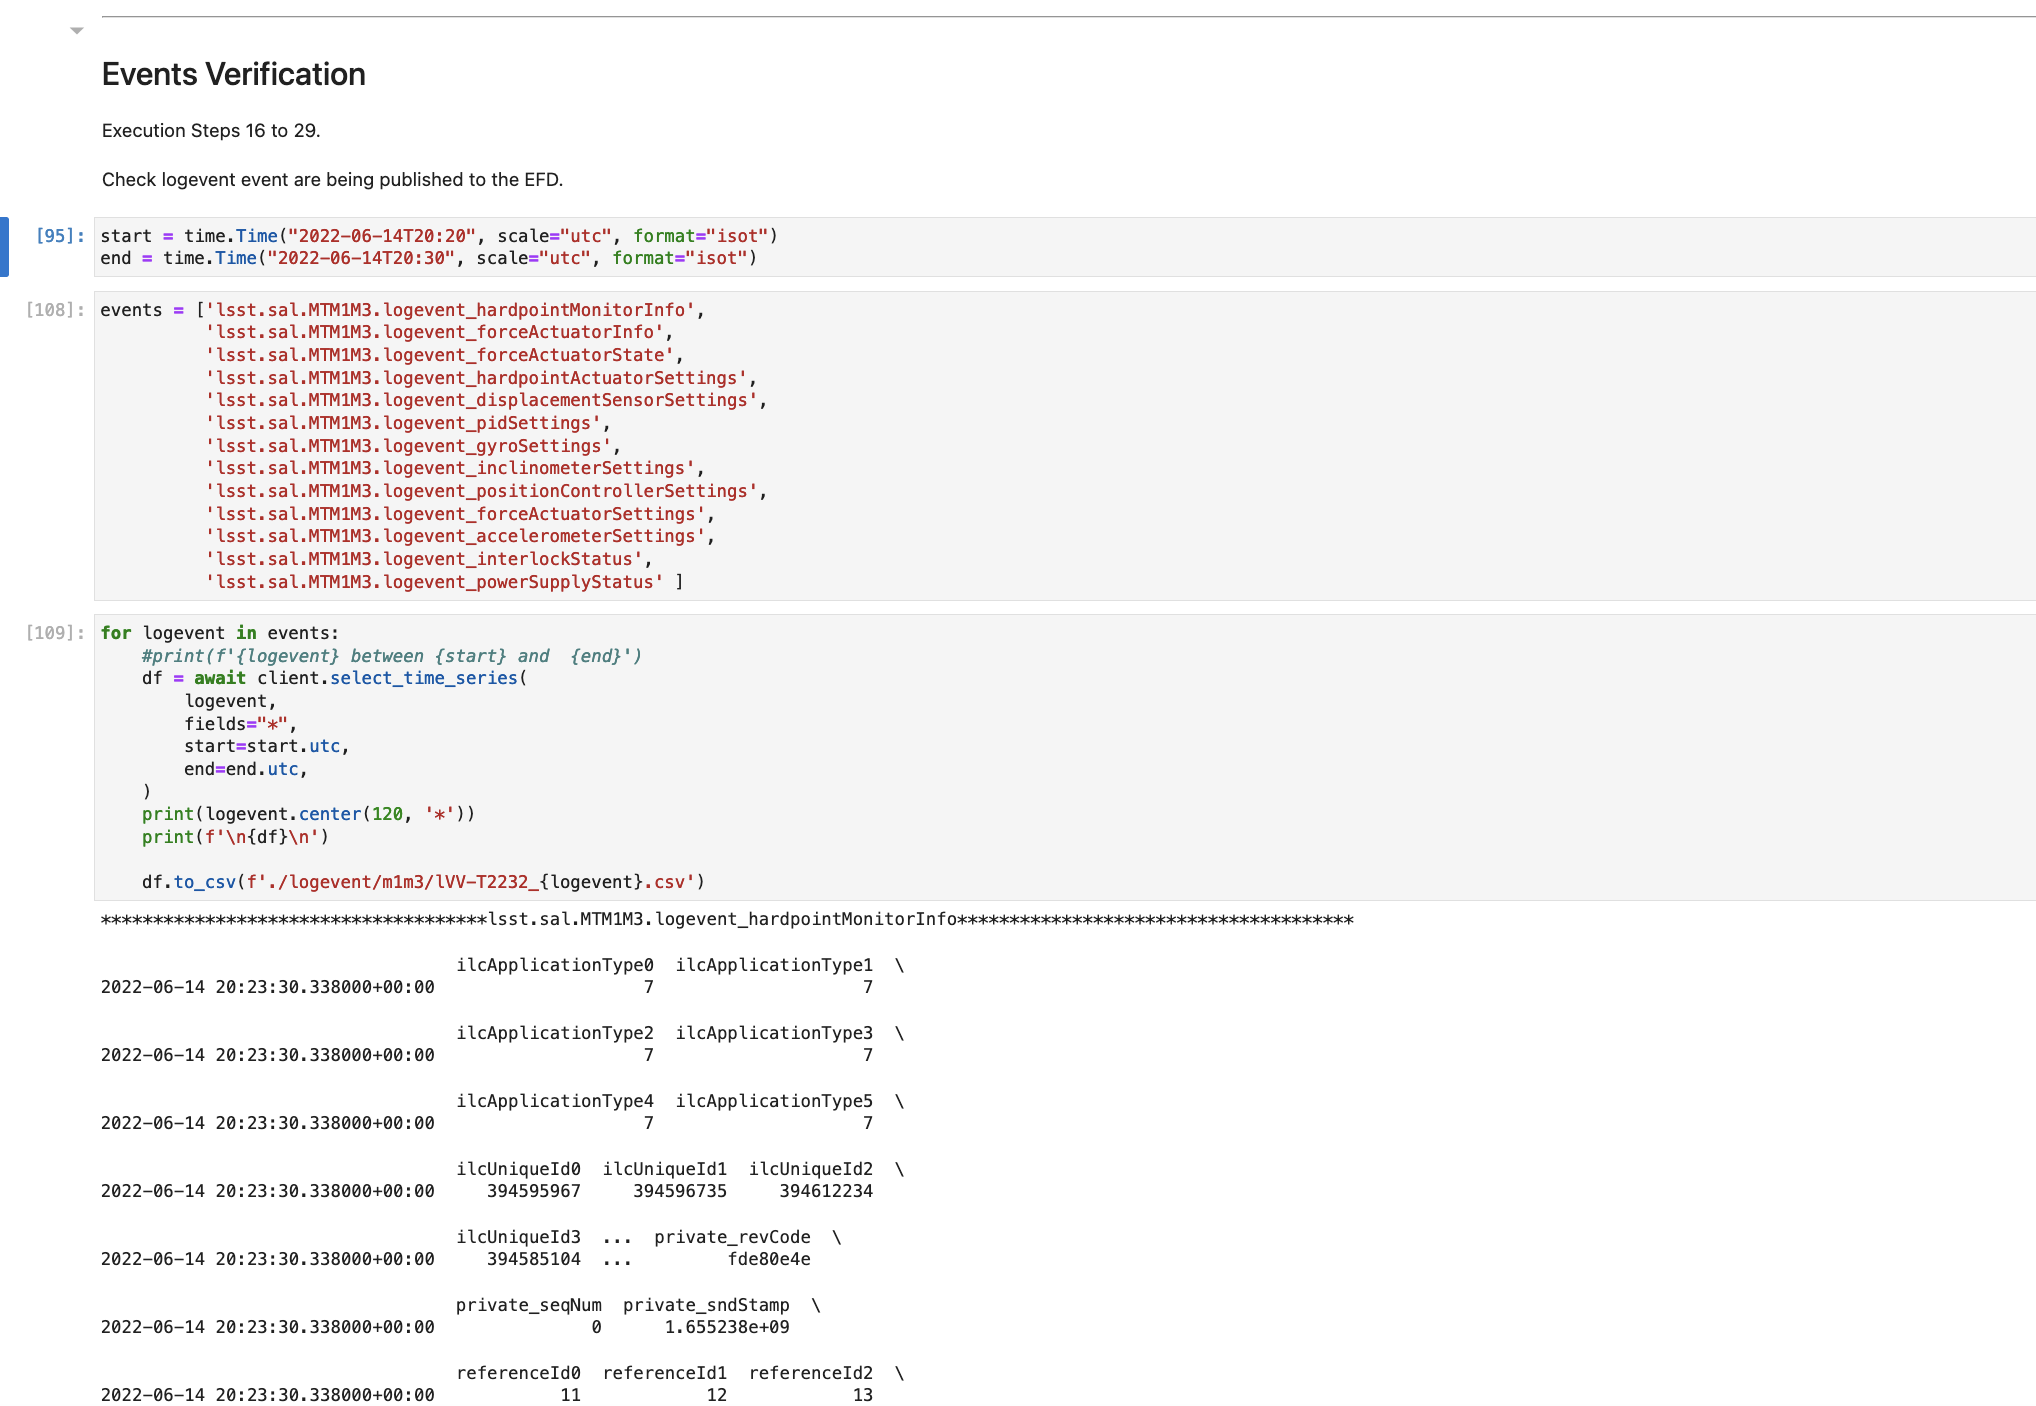
\includegraphics[width=3.12500in]{jira_imgs/2544.png}\\
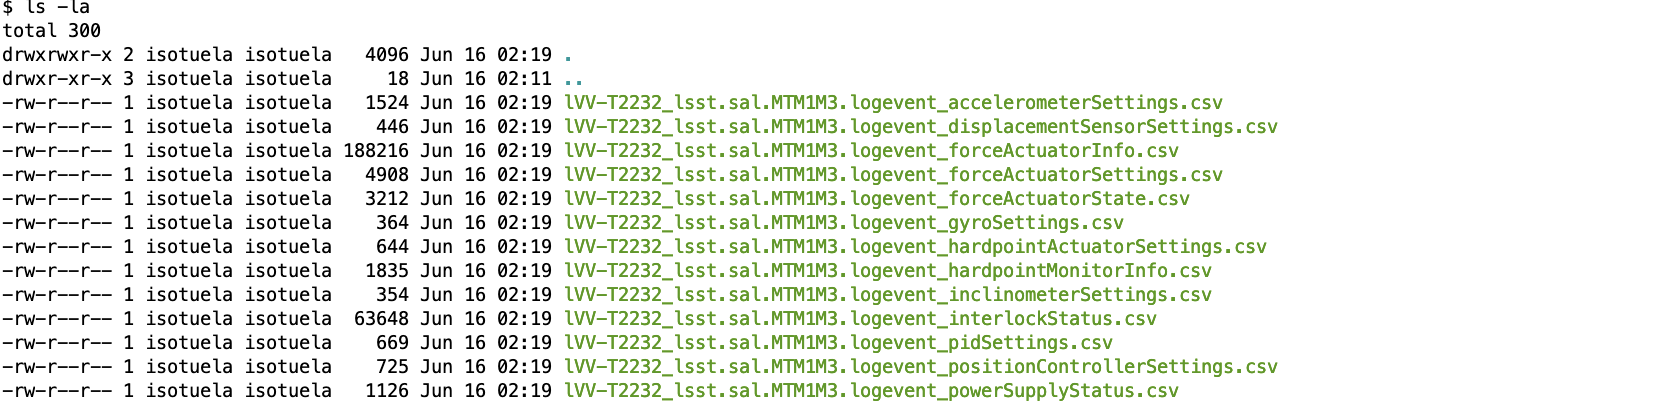
\includegraphics[width=3.12500in]{jira_imgs/2545.png}

}
\begin{tabular}{p{2cm}p{14cm}}
\toprule
Step 18 & Step Execution Status: \textbf{ Pass } \\ \hline
\end{tabular}
 Description \\
{\footnotesize
Verify the \emph{MTM1M3\_logevent\_forceActuatorInfo~}event is published
to the EFD.

}
\hdashrule[0.5ex]{\textwidth}{1pt}{3mm}
  Expected Result \\
{\footnotesize
The \emph{MTM1M3\_logevent\_\emph{forceActuatorInfo}} event is published
to the EFD.

}
\hdashrule[0.5ex]{\textwidth}{1pt}{3mm}
  Actual Result \\
{\footnotesize
All logevent from here to Step 29 were satisfactory checked, querying
the EFD from the notebook. The downloaded dataframe was saved in a file.
The list of files is found below, to demonstrate that the queried
telemetry was being published, that is, the file size is different than
0 (fifth column)\\
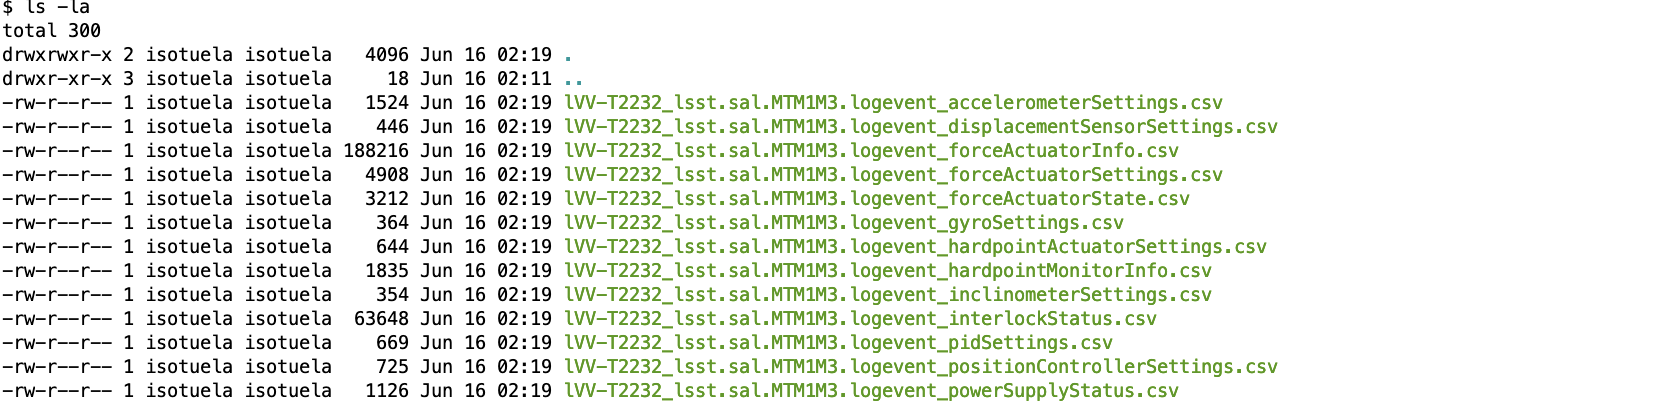
\includegraphics[width=6.31250in]{jira_imgs/2545.png}\\[2\baselineskip]

}
\begin{tabular}{p{2cm}p{14cm}}
\toprule
Step 19 & Step Execution Status: \textbf{ Pass } \\ \hline
\end{tabular}
 Description \\
{\footnotesize
Verify the \emph{MTM1M3\_logevent\_forceActuatorState~}event is
published to the EFD.

}
\hdashrule[0.5ex]{\textwidth}{1pt}{3mm}
  Expected Result \\
{\footnotesize
The \emph{MTM1M3\_logevent\_\emph{forceActuatorState}} event is
published to the EFD.

}
\hdashrule[0.5ex]{\textwidth}{1pt}{3mm}
  Actual Result \\
{\footnotesize
The logevent from Step 16 to Step 29 were succesfully checked with a
query to the EFD from the notebook. The downloaded dataframe was saved
in a file. The list of files is found below, to demonstrate that the
queried telemetry was being published, that is, the file size is
different than 0 (fifth column)\\
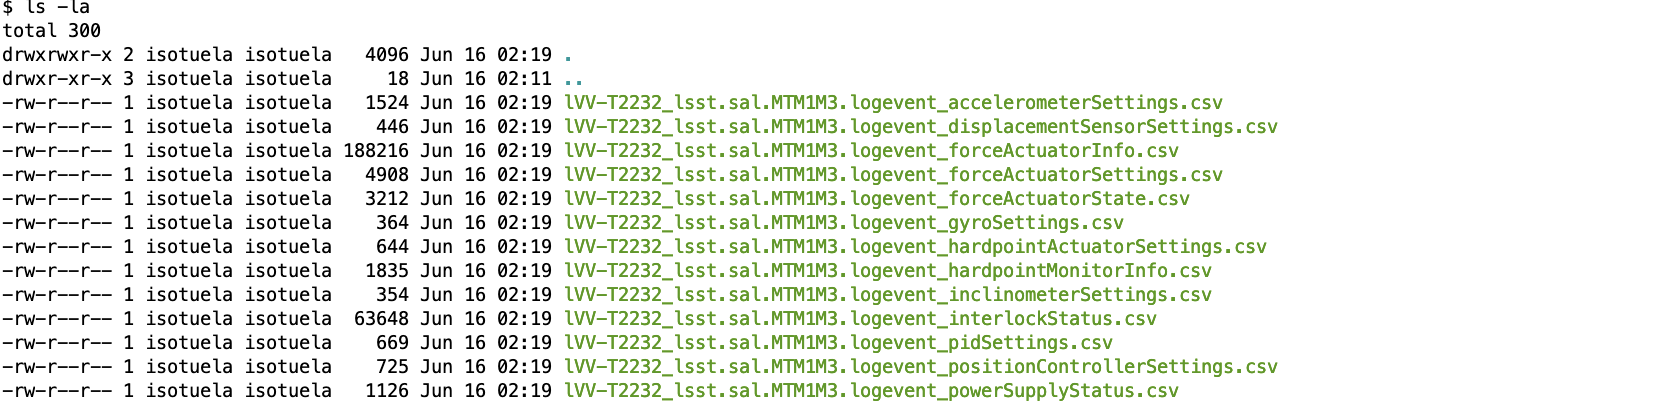
\includegraphics[width=6.88542in]{jira_imgs/2545.png}\\

}
\begin{tabular}{p{2cm}p{14cm}}
\toprule
Step 20 & Step Execution Status: \textbf{ Pass } \\ \hline
\end{tabular}
 Description \\
{\footnotesize
Verify the \emph{MTM1M3\_logevent\_hardpointActuatorSettings~}event is
published to the EFD.

}
\hdashrule[0.5ex]{\textwidth}{1pt}{3mm}
  Expected Result \\
{\footnotesize
The \emph{MTM1M3\_logevent\_\emph{hardpointActuatorSettings}} event is
published to the EFD.

}
\hdashrule[0.5ex]{\textwidth}{1pt}{3mm}
  Actual Result \\
{\footnotesize
The logevent from Step 16 to Step 29 were succesfully checked with a
query to the EFD from the notebook. The downloaded dataframe was saved
in a file. The list of files is found below, to demonstrate that the
queried telemetry was being published, that is, the file size is
different than 0 (fifth column)\\
\includegraphics[width=10.39583in]{jira_imgs/2545.png}\\

}
\begin{tabular}{p{2cm}p{14cm}}
\toprule
Step 21 & Step Execution Status: \textbf{ Pass } \\ \hline
\end{tabular}
 Description \\
{\footnotesize
Verify the \emph{MTM1M3\_logevent\_displacementSensorSettings~}event is
published to the EFD.

}
\hdashrule[0.5ex]{\textwidth}{1pt}{3mm}
  Expected Result \\
{\footnotesize
The \emph{MTM1M3\_logevent\_\emph{displacementSensorSettings}} event is
published to the EFD.

}
\hdashrule[0.5ex]{\textwidth}{1pt}{3mm}
  Actual Result \\
{\footnotesize
The logevent from Step 16 to Step 29 were succesfully checked with a
query to the EFD from the notebook. The downloaded dataframe was saved
in a file. The list of files is found below, to demonstrate that the
queried telemetry was being published, that is, the file size is
different than 0 (fifth column)\\
\includegraphics[width=7.98958in]{jira_imgs/2545.png}\\

}
\begin{tabular}{p{2cm}p{14cm}}
\toprule
Step 22 & Step Execution Status: \textbf{ Pass } \\ \hline
\end{tabular}
 Description \\
{\footnotesize
Verify the \emph{MTM1M3\_logevent\_pidSettings~}event is published to
the EFD.

}
\hdashrule[0.5ex]{\textwidth}{1pt}{3mm}
  Expected Result \\
{\footnotesize
The \emph{MTM1M3\_logevent\_\emph{pidSettings}} event is published to
the EFD.

}
\hdashrule[0.5ex]{\textwidth}{1pt}{3mm}
  Actual Result \\
{\footnotesize
The logevent from Step 16 to Step 29 were succesfully checked with a
query to the EFD from the notebook. The downloaded dataframe was saved
in a file. The list of files is found below, to demonstrate that the
queried telemetry was being published, that is, the file size is
different than 0 (fifth column)\\
\includegraphics[width=6.20833in]{jira_imgs/2545.png}\\

}
\begin{tabular}{p{2cm}p{14cm}}
\toprule
Step 23 & Step Execution Status: \textbf{ Pass } \\ \hline
\end{tabular}
 Description \\
{\footnotesize
Verify the \emph{MTM1M3\_logevent\_gyroSettings~}event is published to
the EFD.

}
\hdashrule[0.5ex]{\textwidth}{1pt}{3mm}
  Expected Result \\
{\footnotesize
The \emph{MTM1M3\_logevent\_\emph{gyroSettings}} event is published to
the EFD.

}
\hdashrule[0.5ex]{\textwidth}{1pt}{3mm}
  Actual Result \\
{\footnotesize
The logevent from Step 16 to Step 29 were succesfully checked with a
query to the EFD from the notebook. The downloaded dataframe was saved
in a file. The list of files is found below, to demonstrate that the
queried telemetry was being published, that is, the file size is
different than 0 (fifth column)\\
\includegraphics[width=5.14583in]{jira_imgs/2545.png}\\

}
\begin{tabular}{p{2cm}p{14cm}}
\toprule
Step 24 & Step Execution Status: \textbf{ Pass } \\ \hline
\end{tabular}
 Description \\
{\footnotesize
Verify the \emph{MTM1M3\_logevent\_inclinometerSettings~}event is
published to the EFD.

}
\hdashrule[0.5ex]{\textwidth}{1pt}{3mm}
  Expected Result \\
{\footnotesize
The \emph{MTM1M3\_logevent\_\emph{inclinometerSettings}} event is
published to the EFD.

}
\hdashrule[0.5ex]{\textwidth}{1pt}{3mm}
  Actual Result \\
{\footnotesize
The logevent from Step 16 to Step 29 were succesfully checked with a
query to the EFD from the notebook. The downloaded dataframe was saved
in a file. The list of files is found below, to demonstrate that the
queried telemetry was being published, that is, the file size is
different than 0 (fifth column)\\
\includegraphics[width=5.27083in]{jira_imgs/2545.png}\\

}
\begin{tabular}{p{2cm}p{14cm}}
\toprule
Step 25 & Step Execution Status: \textbf{ Pass } \\ \hline
\end{tabular}
 Description \\
{\footnotesize
Verify the \emph{MTM1M3\_logevent\_positionControllerSettings~}event is
published to the EFD.

}
\hdashrule[0.5ex]{\textwidth}{1pt}{3mm}
  Expected Result \\
{\footnotesize
The \emph{MTM1M3\_logevent\_\emph{positionControllerSettings}} event is
published to the EFD.

}
\hdashrule[0.5ex]{\textwidth}{1pt}{3mm}
  Actual Result \\
{\footnotesize
The logevent from Step 16 to Step 29 were succesfully checked with a
query to the EFD from the notebook. The downloaded dataframe was saved
in a file. The list of files is found below, to demonstrate that the
queried telemetry was being published, that is, the file size is
different than 0 (fifth column)\\
\includegraphics[width=5.89583in]{jira_imgs/2545.png}\\

}
\begin{tabular}{p{2cm}p{14cm}}
\toprule
Step 26 & Step Execution Status: \textbf{ Pass } \\ \hline
\end{tabular}
 Description \\
{\footnotesize
Verify the \emph{MTM1M3\_logevent\_forceActuatorSettings~}event is
published to the EFD.

}
\hdashrule[0.5ex]{\textwidth}{1pt}{3mm}
  Expected Result \\
{\footnotesize
The \emph{MTM1M3\_logevent\_forceActuatorSettings~}event is published to
the EFD.

}
\hdashrule[0.5ex]{\textwidth}{1pt}{3mm}
  Actual Result \\
{\footnotesize
The logevent from Step 16 to Step 29 were succesfully checked with a
query to the EFD from the notebook. The downloaded dataframe was saved
in a file. The list of files is found below, to demonstrate that the
queried telemetry was being published, that is, the file size is
different than 0 (fifth column)\\
\includegraphics[width=4.80208in]{jira_imgs/2545.png}\\

}
\begin{tabular}{p{2cm}p{14cm}}
\toprule
Step 27 & Step Execution Status: \textbf{ Pass } \\ \hline
\end{tabular}
 Description \\
{\footnotesize
Verify the\emph{~MTM1M3\_logevent\_accelerometerSettings} event is
published to the EFD.

}
\hdashrule[0.5ex]{\textwidth}{1pt}{3mm}
  Expected Result \\
{\footnotesize
The\emph{~\emph{MTM1M3\_logevent\_accelerometerSettings}} event is
published to the EFD.

}
\hdashrule[0.5ex]{\textwidth}{1pt}{3mm}
  Actual Result \\
{\footnotesize
The logevent from Step 16 to Step 29 were succesfully checked with a
query to the EFD from the notebook. The downloaded dataframe was saved
in a file. The list of files is found below, to demonstrate that the
queried telemetry was being published, that is, the file size is
different than 0 (fifth column)\\
\includegraphics[width=4.94792in]{jira_imgs/2545.png}\\

}
\begin{tabular}{p{2cm}p{14cm}}
\toprule
Step 28 & Step Execution Status: \textbf{ Pass } \\ \hline
\end{tabular}
 Description \\
{\footnotesize
Verify the\emph{~MTM1M3\_logevent\_\emph{interlockStatus}} event is
published to the EFD.

}
\hdashrule[0.5ex]{\textwidth}{1pt}{3mm}
  Expected Result \\
{\footnotesize
The\emph{~MTM1M3\_logevent\_\emph{interlockStatus}} event is published
to the EFD.

}
\hdashrule[0.5ex]{\textwidth}{1pt}{3mm}
  Actual Result \\
{\footnotesize
The logevent from Step 16 to Step 29 were succesfully checked with a
query to the EFD from the notebook. The downloaded dataframe was saved
in a file. The list of files is found below, to demonstrate that the
queried telemetry was being published, that is, the file size is
different than 0 (fifth column)\\
\includegraphics[width=5.23958in]{jira_imgs/2545.png}\\

}
\begin{tabular}{p{2cm}p{14cm}}
\toprule
Step 29 & Step Execution Status: \textbf{ Pass } \\ \hline
\end{tabular}
 Description \\
{\footnotesize
Verify the\emph{~MTM1M3\_logevent\_\emph{powerSupplyStatus}} event is
published to the EFD.

}
\hdashrule[0.5ex]{\textwidth}{1pt}{3mm}
  Expected Result \\
{\footnotesize
The\emph{~MTM1M3\_logevent\_\emph{\emph{powerSupplyStatu}s}} event is
published to the EFD.

}
\hdashrule[0.5ex]{\textwidth}{1pt}{3mm}
  Actual Result \\
{\footnotesize
The logevent from Step 16 to Step 29 were succesfully checked with a
query to the EFD from the notebook. The downloaded dataframe was saved
in a file. The list of files is found below, to demonstrate that the
queried telemetry was being published, that is, the file size is
different than 0 (fifth column)\\
\includegraphics[width=4.46875in]{jira_imgs/2545.png}\\

}
\begin{tabular}{p{2cm}p{14cm}}
\toprule
Step 30 & Step Execution Status: \textbf{ Fail } \\ \hline
\end{tabular}
 Description \\
{\footnotesize
\textbf{Warning Events}\\
Verify the \emph{MTM1M3\_logevent\_airSupplyWarning~}event is published
to the EFD.

}
\hdashrule[0.5ex]{\textwidth}{1pt}{3mm}
  Test Data \\
 {\footnotesize
\textbf{Note:} The following steps are meant to verify the warning
events are being published to the EFD via SAL, not as a result of an
actual warning.~

}
\hdashrule[0.5ex]{\textwidth}{1pt}{3mm}
  Expected Result \\
{\footnotesize
The \emph{MTM1M3\_logevent\_\emph{airSupplyWarning}} event is published
to the EFD.

}
\hdashrule[0.5ex]{\textwidth}{1pt}{3mm}
  Actual Result \\
{\footnotesize
Not published to the EFD during the test case execution, but there were
instances in the last month, when this warning was apparently trigered
and published.\\[2\baselineskip]

}
\begin{tabular}{p{2cm}p{14cm}}
\toprule
Step 31 & Step Execution Status: \textbf{ Pass } \\ \hline
\end{tabular}
 Description \\
{\footnotesize
Verify the \emph{MTM1M3\_logevent\_ilcWarning~}event is published to the
EFD.

}
\hdashrule[0.5ex]{\textwidth}{1pt}{3mm}
  Expected Result \\
{\footnotesize
The \emph{MTM1M3\_logevent\_\emph{ilcWarning}} event is published to the
EFD.

}
\hdashrule[0.5ex]{\textwidth}{1pt}{3mm}
  Actual Result \\
{\footnotesize
\includegraphics[width=4.37500in]{jira_imgs/2547.png}\\
\includegraphics[width=5.16667in]{jira_imgs/2546.png}\\

}
\begin{tabular}{p{2cm}p{14cm}}
\toprule
Step 32 & Step Execution Status: \textbf{ Pass } \\ \hline
\end{tabular}
 Description \\
{\footnotesize
Verify the \emph{MTM1M3\_logevent\_forceActuatorWarning~}event is
published to the EFD.

}
\hdashrule[0.5ex]{\textwidth}{1pt}{3mm}
  Expected Result \\
{\footnotesize
The \emph{MTM1M3\_logevent\_forceActuatorWarning~}event is published to
the EFD.

}
\hdashrule[0.5ex]{\textwidth}{1pt}{3mm}
  Actual Result \\
{\footnotesize
Event published to the EFD.\\
\includegraphics[width=5.28125in]{jira_imgs/2546.png}\\

}
\begin{tabular}{p{2cm}p{14cm}}
\toprule
Step 33 & Step Execution Status: \textbf{ Pass } \\ \hline
\end{tabular}
 Description \\
{\footnotesize
Verify the\emph{~MTM1M3\_logevent\_\emph{interlockWarning}} event is
published to the EFD.

}
\hdashrule[0.5ex]{\textwidth}{1pt}{3mm}
  Expected Result \\
{\footnotesize
The\emph{~MTM1M3\_logevent\_\emph{interlockWarning}} event is published
to the EFD.

}
\hdashrule[0.5ex]{\textwidth}{1pt}{3mm}
  Actual Result \\
{\footnotesize
Event seen in the EFD.\\
\includegraphics[width=4.78125in]{jira_imgs/2546.png}\\[3\baselineskip]

}
\begin{tabular}{p{2cm}p{14cm}}
\toprule
Step 34 & Step Execution Status: \textbf{ Fail } \\ \hline
\end{tabular}
 Description \\
{\footnotesize
Verify the\emph{~MTM1M3\_logevent\_\emph{displacementSensorWarning}}
event is published to the EFD.

}
\hdashrule[0.5ex]{\textwidth}{1pt}{3mm}
  Expected Result \\
{\footnotesize
The\emph{~MTM1M3\_logevent\_\emph{\emph{displacementSensorWarning}}}
event is published to the EFD.

}
\hdashrule[0.5ex]{\textwidth}{1pt}{3mm}
  Actual Result \\
{\footnotesize
Not published to the EFD during the test case execution time window.
(File size 3 bytes)\\
\$ cat
lVV-T2232\_lsst.sal.MTM1M3.logevent\_displacementSensorWarning.csv\\
``''\\
\includegraphics[width=4.78125in]{jira_imgs/2548.png}\\

}
\begin{tabular}{p{2cm}p{14cm}}
\toprule
Step 35 & Step Execution Status: \textbf{ Fail } \\ \hline
\end{tabular}
 Description \\
{\footnotesize
Verify the\emph{~MTM1M3\_logevent\_\emph{inclinometerSensorWarning}}
event is published to the EFD.

}
\hdashrule[0.5ex]{\textwidth}{1pt}{3mm}
  Expected Result \\
{\footnotesize
The\emph{~MTM1M3\_logevent\_\emph{\emph{inclinometerSensorWarning}}}
event is published to the EFD.

}
\hdashrule[0.5ex]{\textwidth}{1pt}{3mm}
  Actual Result \\
{\footnotesize
Not published to the EFD during the test case execution time window.
(File size 3 bytes)\\
\$ cat
lVV-T2232\_lsst.sal.MTM1M3.logevent\_inclinometerSensorWarning.csv\\
``''\\
\includegraphics[width=6.37500in]{jira_imgs/2548.png}\\

}
\begin{tabular}{p{2cm}p{14cm}}
\toprule
Step 36 & Step Execution Status: \textbf{ Fail } \\ \hline
\end{tabular}
 Description \\
{\footnotesize
Verify the\emph{~MTM1M3\_logevent\_\emph{accelerometerWarning}} event is
published to the EFD.

}
\hdashrule[0.5ex]{\textwidth}{1pt}{3mm}
  Expected Result \\
{\footnotesize
The\emph{~MTM1M3\_logevent\_\emph{\emph{accelerometerWarning}}} event is
published to the EFD.

}
\hdashrule[0.5ex]{\textwidth}{1pt}{3mm}
  Actual Result \\
{\footnotesize
Not published to the EFD during the test case execution time window.
(File size 3 bytes)\\
\$ cat lVV-T2232\_lsst.sal.MTM1M3.logevent\_accelerometerWarning.csv\\
``''\\
\includegraphics[width=6.69792in]{jira_imgs/2548.png}\\

}
\begin{tabular}{p{2cm}p{14cm}}
\toprule
Step 37 & Step Execution Status: \textbf{ Pass } \\ \hline
\end{tabular}
 Description \\
{\footnotesize
Verify the\emph{~MTM1M3\_logevent\_\emph{forceSetpointWarning}} event is
published to the EFD.

}
\hdashrule[0.5ex]{\textwidth}{1pt}{3mm}
  Expected Result \\
{\footnotesize
The\emph{~MTM1M3\_logevent\_\emph{\emph{forceSetpointWarning}}} event is
published to the EFD.

}
\hdashrule[0.5ex]{\textwidth}{1pt}{3mm}
  Actual Result \\
{\footnotesize
Available in the
EFD\\[2\baselineskip]\includegraphics[width=5.93750in]{jira_imgs/2548.png}\\

}
\begin{tabular}{p{2cm}p{14cm}}
\toprule
Step 38 & Step Execution Status: \textbf{ Fail } \\ \hline
\end{tabular}
 Description \\
{\footnotesize
Verify the\emph{~MTM1M3\_logevent\_\emph{gyroWarning}} event is
published to the EFD.

}
\hdashrule[0.5ex]{\textwidth}{1pt}{3mm}
  Expected Result \\
{\footnotesize
The\emph{~MTM1M3\_logevent\_\emph{\emph{gyroWarning}}} event is
published to the EFD.

}
\hdashrule[0.5ex]{\textwidth}{1pt}{3mm}
  Actual Result \\
{\footnotesize
Empty logevent during the test case execution time window. (File size 3
bytes)\\[2\baselineskip]\includegraphics[width=7.81250in]{jira_imgs/2548.png}\\

}
\begin{tabular}{p{2cm}p{14cm}}
\toprule
Step 39 & Step Execution Status: \textbf{ Pass } \\ \hline
\end{tabular}
 Description \\
{\footnotesize
Verify the\emph{~MTM1M3\_logevent\_forceActuatorForceWarning} event is
published to the EFD.

}
\hdashrule[0.5ex]{\textwidth}{1pt}{3mm}
  Expected Result \\
{\footnotesize
The\emph{~\emph{MTM1M3\_logevent\_forceActuatorForceWarning}} event is
published to the EFD.

}
\hdashrule[0.5ex]{\textwidth}{1pt}{3mm}
  Actual Result \\
{\footnotesize
Published to the
EFD\\[2\baselineskip]\includegraphics[width=1.56250in]{jira_imgs/2548.png}\\

}
\begin{tabular}{p{2cm}p{14cm}}
\toprule
Step 40 & Step Execution Status: \textbf{ Not Executed } \\ \hline
\end{tabular}
 Description \\
{\footnotesize
\textbf{Preclipped Events}\\
Verify the \emph{MTM1M3\_logevent\_preclippedStaticForces~}event is
published to the EFD.

}
\hdashrule[0.5ex]{\textwidth}{1pt}{3mm}
  Test Data \\
 {\footnotesize
\textbf{Note:~}At startup, a configuration file is loaded onto the
system. Verify that the preclipped Events are all published to the EFD
with the same values contained in the configuration file.

}
\hdashrule[0.5ex]{\textwidth}{1pt}{3mm}
  Expected Result \\
{\footnotesize
The \emph{MTM1M3\_logevent\_preclippedStaticForces~}event is published
to the EFD.

}
\hdashrule[0.5ex]{\textwidth}{1pt}{3mm}
  Actual Result \\
{\footnotesize
Preclipped events are only published when the first component of the
M1M3 forces is out of limit and needs to be preclipped.

}
\begin{tabular}{p{2cm}p{14cm}}
\toprule
Step 41 & Step Execution Status: \textbf{ Not Executed } \\ \hline
\end{tabular}
 Description \\
{\footnotesize
Verify the \emph{MTM1M3\_logevent\_appliedStaticForces~}event is
published to the EFD.

}
\hdashrule[0.5ex]{\textwidth}{1pt}{3mm}
  Expected Result \\
{\footnotesize
The \emph{MTM1M3\_logevent\_\emph{appliedStaticForces}} event is
published to the EFD.

}
\hdashrule[0.5ex]{\textwidth}{1pt}{3mm}
  Actual Result \\
{\footnotesize

}
\begin{tabular}{p{2cm}p{14cm}}
\toprule
Step 42 & Step Execution Status: \textbf{ Not Executed } \\ \hline
\end{tabular}
 Description \\
{\footnotesize
Verify the
\emph{MTM1M3\_logevent\_\emph{\emph{preclipped}ElevationForces}~}event
is published to the EFD.

}
\hdashrule[0.5ex]{\textwidth}{1pt}{3mm}
  Expected Result \\
{\footnotesize
The
\emph{MTM1M3\_logevent\_\emph{\emph{\emph{preclipped}ElevationForces}}~}event
is published to the EFD.

}
\hdashrule[0.5ex]{\textwidth}{1pt}{3mm}
  Actual Result \\
{\footnotesize
Preclipped events are only published when the first component of the
M1M3 forces is out of limit and needs to be preclipped.

}
\begin{tabular}{p{2cm}p{14cm}}
\toprule
Step 43 & Step Execution Status: \textbf{ Not Executed } \\ \hline
\end{tabular}
 Description \\
{\footnotesize
Verify the
\emph{MTM1M3\_logevent\_\emph{\emph{preclipped}AzimuthForces}~}event is
published to the EFD.

}
\hdashrule[0.5ex]{\textwidth}{1pt}{3mm}
  Expected Result \\
{\footnotesize
The
\emph{MTM1M3\_logevent\_\emph{\emph{\emph{preclipped}AzimuthForces~}}}event
is published to the EFD.

}
\hdashrule[0.5ex]{\textwidth}{1pt}{3mm}
  Actual Result \\
{\footnotesize
Preclipped events are only published when the first component of the
M1M3 forces is out of limit and needs to be preclipped.

}
\begin{tabular}{p{2cm}p{14cm}}
\toprule
Step 44 & Step Execution Status: \textbf{ Not Executed } \\ \hline
\end{tabular}
 Description \\
{\footnotesize
Verify the
\emph{MTM1M3\_logevent\_\emph{\emph{preclipped}ThermalForces}~}event is
published to the EFD.

}
\hdashrule[0.5ex]{\textwidth}{1pt}{3mm}
  Expected Result \\
{\footnotesize
The
\emph{MTM1M3\_logevent\_\emph{\emph{\emph{preclipped}ThermalForces}}~}event
is published to the EFD.

}
\hdashrule[0.5ex]{\textwidth}{1pt}{3mm}
  Actual Result \\
{\footnotesize
Preclipped events are only published when the first component of the
M1M3 forces is out of limit and needs to be preclipped.

}
\begin{tabular}{p{2cm}p{14cm}}
\toprule
Step 45 & Step Execution Status: \textbf{ Not Executed } \\ \hline
\end{tabular}
 Description \\
{\footnotesize
Verify the
\emph{MTM1M3\_logevent\_\emph{\emph{preclippedActiveOptic}Forces}~}event
is published to the EFD.

}
\hdashrule[0.5ex]{\textwidth}{1pt}{3mm}
  Expected Result \\
{\footnotesize
The
\emph{MTM1M3\_logevent\_\emph{\emph{\emph{preclippedActiveOptic}Forces}}~}event
is published to the EFD.

}
\hdashrule[0.5ex]{\textwidth}{1pt}{3mm}
  Actual Result \\
{\footnotesize
Preclipped events are only published when the first component of the
M1M3 forces is out of limit and needs to be preclipped.

}
\begin{tabular}{p{2cm}p{14cm}}
\toprule
Step 46 & Step Execution Status: \textbf{ Not Executed } \\ \hline
\end{tabular}
 Description \\
{\footnotesize
Verify the \emph{MTM1M3\_logevent\_\emph{preclippedBalanceForces}~}event
is published to the EFD.

}
\hdashrule[0.5ex]{\textwidth}{1pt}{3mm}
  Expected Result \\
{\footnotesize
The \emph{MTM1M3\_logevent\_\emph{\emph{preclippedBalanceForces}}~}event
is published to the EFD.

}
\hdashrule[0.5ex]{\textwidth}{1pt}{3mm}
  Actual Result \\
{\footnotesize
Preclipped events are only published when the first component of the
M1M3 forces is out of limit and needs to be preclipped.

}
\begin{tabular}{p{2cm}p{14cm}}
\toprule
Step 47 & Step Execution Status: \textbf{ Not Executed } \\ \hline
\end{tabular}
 Description \\
{\footnotesize
Verify the
\emph{MTM1M3\_logevent\_\emph{preclippedVelocityForces}~}event is
published to the EFD.

}
\hdashrule[0.5ex]{\textwidth}{1pt}{3mm}
  Expected Result \\
{\footnotesize
The
\emph{MTM1M3\_logevent\_\emph{\emph{preclippedVelocityForces}}~}event is
published to the EFD.

}
\hdashrule[0.5ex]{\textwidth}{1pt}{3mm}
  Actual Result \\
{\footnotesize
Preclipped events are only published when the first component of the
M1M3 forces is out of limit and needs to be preclipped.

}
\begin{tabular}{p{2cm}p{14cm}}
\toprule
Step 48 & Step Execution Status: \textbf{ Not Executed } \\ \hline
\end{tabular}
 Description \\
{\footnotesize
Verify the
\emph{MTM1M3\_logevent\_\emph{preclippedAccelerationForces}~}event is
published to the EFD.

}
\hdashrule[0.5ex]{\textwidth}{1pt}{3mm}
  Expected Result \\
{\footnotesize
The
\emph{MTM1M3\_logevent\_\emph{\emph{preclippedAccelerationForces}}~}event
is published to the EFD.

}
\hdashrule[0.5ex]{\textwidth}{1pt}{3mm}
  Actual Result \\
{\footnotesize
Preclipped events are only published when the first component of the
M1M3 forces is out of limit and needs to be preclipped.

}
\begin{tabular}{p{2cm}p{14cm}}
\toprule
Step 49 & Step Execution Status: \textbf{ Not Executed } \\ \hline
\end{tabular}
 Description \\
{\footnotesize
Verify the \emph{MTM1M3\_logevent\_\emph{preclippedOffsetForces}~}event
is published to the EFD.

}
\hdashrule[0.5ex]{\textwidth}{1pt}{3mm}
  Expected Result \\
{\footnotesize
The \emph{MTM1M3\_logevent\_\emph{\emph{preclippedOffsetForces}}~}event
is published to the EFD.

}
\hdashrule[0.5ex]{\textwidth}{1pt}{3mm}
  Actual Result \\
{\footnotesize
Preclipped events are only published when the first component of the
M1M3 forces is out of limit and needs to be preclipped.

}
\begin{tabular}{p{2cm}p{14cm}}
\toprule
Step 50 & Step Execution Status: \textbf{ Not Executed } \\ \hline
\end{tabular}
 Description \\
{\footnotesize
Verify the
\emph{MTM1M3\_logevent\_\emph{preclippedCylinderForces}~}event is
published to the EFD.

}
\hdashrule[0.5ex]{\textwidth}{1pt}{3mm}
  Expected Result \\
{\footnotesize
The
\emph{MTM1M3\_logevent\_\emph{\emph{preclippedCylinderForces}}~}event is
published to the EFD.

}
\hdashrule[0.5ex]{\textwidth}{1pt}{3mm}
  Actual Result \\
{\footnotesize
Preclipped events are only published when the first component of the
M1M3 forces is out of limit and needs to be preclipped.

}
\begin{tabular}{p{2cm}p{14cm}}
\toprule
Step 51 & Step Execution Status: \textbf{ Not Executed } \\ \hline
\end{tabular}
 Description \\
{\footnotesize
Verify the \emph{MTM1M3\_logevent\_\emph{preclippedForces}~}event is
published to the EFD.

}
\hdashrule[0.5ex]{\textwidth}{1pt}{3mm}
  Expected Result \\
{\footnotesize
The \emph{MTM1M3\_logevent\_\emph{\emph{preclippedForces}}~}event is
published to the EFD.

}
\hdashrule[0.5ex]{\textwidth}{1pt}{3mm}
  Actual Result \\
{\footnotesize
Preclipped events are only published when the first component of the
M1M3 forces is out of limit and needs to be preclipped.

}
\begin{tabular}{p{2cm}p{14cm}}
\toprule
Step 52 & Step Execution Status: \textbf{ Not Executed } \\ \hline
\end{tabular}
 Description \\
{\footnotesize
\textbf{Applied Events}\\
Verify the \emph{MTM1M3\_logevent\_\emph{appliedAccelerationForces}}
event is published to the EFD.

}
\hdashrule[0.5ex]{\textwidth}{1pt}{3mm}
  Test Data \\
 {\footnotesize
\textbf{Note:~}Similar to the preclipped events, the following steps are
meant to verify that the events have been published to the EFD via SAL.

}
\hdashrule[0.5ex]{\textwidth}{1pt}{3mm}
  Expected Result \\
{\footnotesize
The\emph{~MTM1M3\_logevent\_\emph{appliedAccelerationForces}} event is
published to the EFD.

}
\hdashrule[0.5ex]{\textwidth}{1pt}{3mm}
  Actual Result \\
{\footnotesize

}
\begin{tabular}{p{2cm}p{14cm}}
\toprule
Step 53 & Step Execution Status: \textbf{ Not Executed } \\ \hline
\end{tabular}
 Description \\
{\footnotesize
Verify the \emph{MTM1M3\_logevent\_\emph{appliedThermalForces}} event is
published to the EFD.

}
\hdashrule[0.5ex]{\textwidth}{1pt}{3mm}
  Expected Result \\
{\footnotesize
The\emph{~MTM1M3\_logevent\_\emph{\emph{appliedThermalForces}}} event is
published to the EFD.

}
\hdashrule[0.5ex]{\textwidth}{1pt}{3mm}
  Actual Result \\
{\footnotesize

}
\begin{tabular}{p{2cm}p{14cm}}
\toprule
Step 54 & Step Execution Status: \textbf{ Not Executed } \\ \hline
\end{tabular}
 Description \\
{\footnotesize
Verify the \emph{MTM1M3\_logevent\_\emph{appliedVelocityForces}} event
is published to the EFD.

}
\hdashrule[0.5ex]{\textwidth}{1pt}{3mm}
  Expected Result \\
{\footnotesize
The\emph{~MTM1M3\_logevent\_\emph{\emph{appliedVelocityForces}}} event
is published to the EFD.

}
\hdashrule[0.5ex]{\textwidth}{1pt}{3mm}
  Actual Result \\
{\footnotesize

}
\begin{tabular}{p{2cm}p{14cm}}
\toprule
Step 55 & Step Execution Status: \textbf{ Not Executed } \\ \hline
\end{tabular}
 Description \\
{\footnotesize
Verify the \emph{MTM1M3\_logevent\_\emph{appliedBalanceForces}} event is
published to the EFD.

}
\hdashrule[0.5ex]{\textwidth}{1pt}{3mm}
  Expected Result \\
{\footnotesize
The\emph{~MTM1M3\_logevent\_\emph{\emph{appliedBalanceForces}}} event is
published to the EFD.

}
\hdashrule[0.5ex]{\textwidth}{1pt}{3mm}
  Actual Result \\
{\footnotesize

}
\begin{tabular}{p{2cm}p{14cm}}
\toprule
Step 56 & Step Execution Status: \textbf{ Not Executed } \\ \hline
\end{tabular}
 Description \\
{\footnotesize
Verify the \emph{MTM1M3\_logevent\_\emph{appliedCylinderForces}} event
is published to the EFD.

}
\hdashrule[0.5ex]{\textwidth}{1pt}{3mm}
  Expected Result \\
{\footnotesize
The\emph{~MTM1M3\_logevent\_\emph{\emph{appliedCylinderForces}}} event
is published to the EFD.

}
\hdashrule[0.5ex]{\textwidth}{1pt}{3mm}
  Actual Result \\
{\footnotesize

}
\begin{tabular}{p{2cm}p{14cm}}
\toprule
Step 57 & Step Execution Status: \textbf{ Not Executed } \\ \hline
\end{tabular}
 Description \\
{\footnotesize
Verify the \emph{MTM1M3\_logevent\_\emph{appliedForces}} event is
published to the EFD.

}
\hdashrule[0.5ex]{\textwidth}{1pt}{3mm}
  Expected Result \\
{\footnotesize
The\emph{~MTM1M3\_logevent\_\emph{\emph{appliedForces}}} event is
published to the EFD.

}
\hdashrule[0.5ex]{\textwidth}{1pt}{3mm}
  Actual Result \\
{\footnotesize

}
\begin{tabular}{p{2cm}p{14cm}}
\toprule
Step 58 & Step Execution Status: \textbf{ Not Executed } \\ \hline
\end{tabular}
 Description \\
{\footnotesize
Verify the \emph{MTM1M3\_logevent\_\emph{appliedStaticForces}} event is
published to the EFD.

}
\hdashrule[0.5ex]{\textwidth}{1pt}{3mm}
  Expected Result \\
{\footnotesize
The\emph{~MTM1M3\_logevent\_\emph{\emph{appliedStaticForces}}} event is
published to the EFD.

}
\hdashrule[0.5ex]{\textwidth}{1pt}{3mm}
  Actual Result \\
{\footnotesize

}
\begin{tabular}{p{2cm}p{14cm}}
\toprule
Step 59 & Step Execution Status: \textbf{ Not Executed } \\ \hline
\end{tabular}
 Description \\
{\footnotesize
Verify the\emph{~MTM1M3\_logevent\_\emph{appliedAzimuthForces}} event is
published to the EFD.

}
\hdashrule[0.5ex]{\textwidth}{1pt}{3mm}
  Expected Result \\
{\footnotesize
The\emph{~MTM1M3\_logevent\_\emph{\emph{appliedAzimuthForces}}} event is
published to the EFD.

}
\hdashrule[0.5ex]{\textwidth}{1pt}{3mm}
  Actual Result \\
{\footnotesize

}
\begin{tabular}{p{2cm}p{14cm}}
\toprule
Step 60 & Step Execution Status: \textbf{ Not Executed } \\ \hline
\end{tabular}
 Description \\
{\footnotesize
Verify the\emph{~MTM1M3\_logevent\_\emph{appliedElevationForces}} event
is published to the EFD.

}
\hdashrule[0.5ex]{\textwidth}{1pt}{3mm}
  Expected Result \\
{\footnotesize
The\emph{~MTM1M3\_logevent\_\emph{appliedElevationForces}} event is
published to the EFD.

}
\hdashrule[0.5ex]{\textwidth}{1pt}{3mm}
  Actual Result \\
{\footnotesize

}
\begin{tabular}{p{2cm}p{14cm}}
\toprule
Step 61 & Step Execution Status: \textbf{ Pass } \\ \hline
\end{tabular}
 Description \\
{\footnotesize
\textbf{Engineering Mode Test}\\
While the M1M3 is enabled and in the PARKED state, send an
\emph{MTM1M3\_command\_enterEngineering} command.

}
\hdashrule[0.5ex]{\textwidth}{1pt}{3mm}
  Expected Result \\
{\footnotesize
The system transitions into the ParkedEngineering state.~

}
\hdashrule[0.5ex]{\textwidth}{1pt}{3mm}
  Actual Result \\
{\footnotesize
We ran the command successfully and checked that it was in
PARKEDENGINEERING using the commands below:\\[2\baselineskip]{from
lsst.ts.idl.enums.MTM1M3 import DetailedState\\
m1m3\_dstate = mtcs.rem.mtm1m3.evt\_detailedState.get()\\
print(DetailedState.PARKEDENGINEERING == m1m3\_dstate.detailedState)}

}
\begin{tabular}{p{2cm}p{14cm}}
\toprule
Step 62 & Step Execution Status: \textbf{ Fail } \\ \hline
\end{tabular}
 Description \\
{\footnotesize
With the system in the ParkedEngineering state and the M1M3 cell lights
off, send an~\emph{MTM1M3\_command\_turnLightsOn} command.

}
\hdashrule[0.5ex]{\textwidth}{1pt}{3mm}
  Test Data \\
 {\footnotesize
Note: If the lights are already on, this command will not do anything.

}
\hdashrule[0.5ex]{\textwidth}{1pt}{3mm}
  Expected Result \\
{\footnotesize
\begin{itemize}
\tightlist
\item
  The M1M3 cell lights turn on.
\item
  The \emph{MTM1M3\_logevent\_cellLightStatus} event is published to the
  EFD.
\item
  The \emph{MTM1M3\_logevent\_cellLightWarning} event is published to
  the EFD to show no warnings.
\end{itemize}

}
\hdashrule[0.5ex]{\textwidth}{1pt}{3mm}
  Actual Result \\
{\footnotesize
The lights were off and we sent the command to turn them on.\\
We verified visually that the \textbf{lights went on.}\\
The cellLightStatus logevent says:\\

\begin{verbatim}
private_revCode: c34d42d2, private_sndStamp: 1655305398.8532453, private_rcvStamp: 1655305398.853845, private_seqNum: 2, private_identity: MTM1M3, private_origin: 11199, timestamp: 1655305398.852754, cellLightsCommandedOn: True, cellLightsOutputOn: True, cellLightsOn: False, priority: 0
\end{verbatim}

The reason why it indicates that the cellLightsOn: False is because the
sensor is not connected. So this field will always tell us that the
lights are off.\\[2\baselineskip]Since we commanded the lights to turn
on and the log says that they are off, we do have a warning:\\

\begin{verbatim}
private_revCode: 8bbed6ea, private_sndStamp: 1655305398.9532137, private_rcvStamp: 1655305398.9538088, private_seqNum: 2, private_identity: MTM1M3, private_origin: 11199, timestamp: 1655305398.9527543, anyWarning: True, cellLightsOutputMismatch: False, cellLightsSensorMismatch: True, priority: 0
\end{verbatim}

}
\hdashrule[0.5ex]{\textwidth}{1pt}{3mm}
  Issues found executing this step:  \\
{\footnotesize
\begin{itemize}
\item \href{https://jira.lsstcorp.org/browse/SUMMIT-6556}{SUMMIT-6556}~~Connect M1M3 cell light relay signalling lights are powered

\end{itemize}
}
\begin{tabular}{p{2cm}p{14cm}}
\toprule
Step 63 & Step Execution Status: \textbf{ Pass } \\ \hline
\end{tabular}
 Description \\
{\footnotesize
With the system in the ParkedEngineering state and the M1M3 cell lights
off, send an~\emph{MTM1M3\_command\_turnLightsOff} command.

}
\hdashrule[0.5ex]{\textwidth}{1pt}{3mm}
  Test Data \\
 {\footnotesize
Note: If the lights are already off, this command will not do anything.

}
\hdashrule[0.5ex]{\textwidth}{1pt}{3mm}
  Expected Result \\
{\footnotesize
\begin{itemize}
\tightlist
\item
  The M1M3 cell lights turn off.
\item
  The \emph{MTM1M3\_logevent\_cellLightStatus} event is published to the
  EFD.
\item
  The \emph{MTM1M3\_logevent\_cellLightWarning} event is published to
  the EFD to show no warnings.
\end{itemize}

}
\hdashrule[0.5ex]{\textwidth}{1pt}{3mm}
  Actual Result \\
{\footnotesize
The lights were on and we sent the command to turn them off.\\
We verified visually that the lights went off.\\
We also used the two log events above to confirm that the lights are off
and that we have no warnings.

}
\begin{tabular}{p{2cm}p{14cm}}
\toprule
Step 64 & Step Execution Status: \textbf{ Fail } \\ \hline
\end{tabular}
 Description \\
{\footnotesize
With the system in the ParkedEngineering state and the telescope is not
moving, send an~\emph{MTM1M3\_command\_setAirSlewFlag} command to open
the booster valves.

}
\hdashrule[0.5ex]{\textwidth}{1pt}{3mm}
  Test Data \\
 {\footnotesize
By default, the booster valves are closed when not slewing.

}
\hdashrule[0.5ex]{\textwidth}{1pt}{3mm}
  Expected Result \\
{\footnotesize
{The command is accepted and the booster valves open.~}

}
\hdashrule[0.5ex]{\textwidth}{1pt}{3mm}
  Actual Result \\
{\footnotesize
The command was issued and accepted successfully.\\[2\baselineskip]In
order to check that something actually happened, we checked the
\textbf{evt\_forceActuatorState} event, slewFlag.\\
If the booster valves are closed, the slewFlag is False. If they are
open, the slewFlag is True.\\
However, even after sending the command, we still see that the slewFlag
is False.~

}
\hdashrule[0.5ex]{\textwidth}{1pt}{3mm}
  Issues found executing this step:  \\
{\footnotesize
\begin{itemize}
\item \href{https://jira.lsstcorp.org/browse/DM-35229}{DM-35229}~~ForceActuatorState doesn't publish slewFlag updates

\end{itemize}
}
\begin{tabular}{p{2cm}p{14cm}}
\toprule
Step 65 & Step Execution Status: \textbf{ Fail } \\ \hline
\end{tabular}
 Description \\
{\footnotesize
In the ParkedEngineering state, send
an~\emph{MTM1M3\_command\_testHardpoint} command.

}
\hdashrule[0.5ex]{\textwidth}{1pt}{3mm}
  Expected Result \\
{\footnotesize
\begin{itemize}
\tightlist
\item
  There are no warnings published to the
  \emph{MTM1M3\_logevent\_hardpointActuatorWarning} event.
\item
  There are no warnings published to the
  \emph{MTM1M3\_logevent\_hardpointMonitorWarning} event.
\item
  The \emph{MTM1M3\_logevent\_hardpointActuatorState} event is published
  to the EFD.
\item
  The \emph{MTM1M3\_logevent\_hardpointMonitorState} event is published
  to the EFD.
\end{itemize}

}
\hdashrule[0.5ex]{\textwidth}{1pt}{3mm}
  Actual Result \\
{\footnotesize
\includegraphics[width=6.83333in]{jira_imgs/2521.png}\\
There is an implementation of the test as a script in but this is not
implemented at the CSC level.\\
Here is the location of the test script:\\
https://github.com/lsst-ts/ts\_m1m3supporttesting/blob/develop/M13T004.py

}
\hdashrule[0.5ex]{\textwidth}{1pt}{3mm}
  Issues found executing this step:  \\
{\footnotesize
\begin{itemize}
\item \href{https://jira.lsstcorp.org/browse/SITCOM-410}{SITCOM-410}~~Decide fate of testHardpoint command (the functionality is provided with
M13T004)

\end{itemize}
}
\begin{tabular}{p{2cm}p{14cm}}
\toprule
Step 66 & Step Execution Status: \textbf{ Pass } \\ \hline
\end{tabular}
 Description \\
{\footnotesize
In the enabled state, send
an~\emph{MTM1M3\_command\_moveHardpointActuators} command.

}
\hdashrule[0.5ex]{\textwidth}{1pt}{3mm}
  Expected Result \\
{\footnotesize
The command is accepted and the hardpoint actuators begin to move.

}
\hdashrule[0.5ex]{\textwidth}{1pt}{3mm}
  Actual Result \\
{\footnotesize
The command was accepted successfully and we confirmed via EFD that the
hardpoints moved.\\
\includegraphics[width=8.27083in]{jira_imgs/2522.png}

}
\begin{tabular}{p{2cm}p{14cm}}
\toprule
Step 67 & Step Execution Status: \textbf{ Pass } \\ \hline
\end{tabular}
 Description \\
{\footnotesize
While the M1M3 is still in motion, send
an~\emph{MTM1M3\_command\_stopHardpointMotion} command.

}
\hdashrule[0.5ex]{\textwidth}{1pt}{3mm}
  Expected Result \\
{\footnotesize
{The command is accepted and the hardpoint does not complete the
previous command.}

}
\hdashrule[0.5ex]{\textwidth}{1pt}{3mm}
  Actual Result \\
{\footnotesize
\# The range of the actuators is up to 64k\\
await
mtcs.rem.mtm1m3.cmd\_moveHardpointActuators.set\_start(steps={[}10000{]}*6)\\
await asyncio.sleep(3)\\
await
mtcs.rem.mtm1m3.cmd\_stopHardpointMotion.set\_start()\\[2\baselineskip]\includegraphics[width=8.44792in]{jira_imgs/2523.png}

}
\begin{tabular}{p{2cm}p{14cm}}
\toprule
Step 68 & Step Execution Status: \textbf{ Pass } \\ \hline
\end{tabular}
 Description \\
{\footnotesize
In the enabled state, send
an~\emph{MTM1M3\_command\_moveHardpointActuators} command.

}
\hdashrule[0.5ex]{\textwidth}{1pt}{3mm}
  Expected Result \\
{\footnotesize
The command is accepted and the hardpoints are move to the specified
number of steps.

}
\hdashrule[0.5ex]{\textwidth}{1pt}{3mm}
  Actual Result \\
{\footnotesize
The command ran successfully. See the drop on the right edge of the plot
below.\\
\includegraphics[width=9.20833in]{jira_imgs/2524.png}

}
\begin{tabular}{p{2cm}p{14cm}}
\toprule
Step 69 & Step Execution Status: \textbf{ Pass } \\ \hline
\end{tabular}
 Description \\
{\footnotesize
\textbf{Enabled Force Actuator Test}\\
Verify the \emph{MTM1M3\_logevent\_enabledForceActuators} event is
published

}
\hdashrule[0.5ex]{\textwidth}{1pt}{3mm}
  Expected Result \\
{\footnotesize
The \emph{MTM1M3\_logevent\_\emph{enabledForceActuators}} event shows
all actuators are enabled

}
\hdashrule[0.5ex]{\textwidth}{1pt}{3mm}
  Actual Result \\
{\footnotesize
We start with all the actuators enabled. M1M3 cannot operate if more
than 3 actuators are disabled.\\
The code below reflects the two steps below.\\[2\baselineskip]await
mtcs.rem.mtm1m3.cmd\_enableForceActuator.set\_start(actuatorId=225)\\
print(
mtcs.rem.mtm1m3.evt\_enabledForceActuators.get().forceActuatorEnabled{[}60{]}
)\\
\# it should say False and it said False\\[2\baselineskip]await
mtcs.rem.mtm1m3.cmd\_enableForceActuator.set\_start(actuatorId=225)\\
print(
mtcs.rem.mtm1m3.evt\_enabledForceActuators.get().forceActuatorEnabled{[}60{]}
)\\
\# it should say True and it said True

}
\begin{tabular}{p{2cm}p{14cm}}
\toprule
Step 70 & Step Execution Status: \textbf{ Pass } \\ \hline
\end{tabular}
 Description \\
{\footnotesize
In the enabled state of the Engineering mode, send
an~\emph{MTM1M3\_command\_disableForceActuator} command.

}
\hdashrule[0.5ex]{\textwidth}{1pt}{3mm}
  Test Data \\
 {\footnotesize
Note: Any single Force actuator can be disabled. For example, use force
actuator 208

}
\hdashrule[0.5ex]{\textwidth}{1pt}{3mm}
  Expected Result \\
{\footnotesize
\begin{itemize}
\tightlist
\item
  The actuator is disabled.
\item
  The telemetry topic \emph{MTM1M3\_forceActuatorData} doesn't update
  the values for the disabled force actuator
\end{itemize}

}
\hdashrule[0.5ex]{\textwidth}{1pt}{3mm}
  Actual Result \\
{\footnotesize
See the step above.

}
\begin{tabular}{p{2cm}p{14cm}}
\toprule
Step 71 & Step Execution Status: \textbf{ Pass } \\ \hline
\end{tabular}
 Description \\
{\footnotesize
In the enabled state of the Engineering mode, send
an~\emph{MTM1M3\_command\_enableForceActuator} command.

}
\hdashrule[0.5ex]{\textwidth}{1pt}{3mm}
  Test Data \\
 {\footnotesize
Note: Enable the same force actuator that was disabled by the previous
step.

}
\hdashrule[0.5ex]{\textwidth}{1pt}{3mm}
  Expected Result \\
{\footnotesize
\begin{itemize}
\tightlist
\item
  The actuator is enabled.
\item
  The telemetry topic \emph{MTM1M3\_forceActuatorData} updates the
  values for the enabled force actuator
\end{itemize}

}
\hdashrule[0.5ex]{\textwidth}{1pt}{3mm}
  Actual Result \\
{\footnotesize
See the step above.

}
\begin{tabular}{p{2cm}p{14cm}}
\toprule
Step 72 & Step Execution Status: \textbf{ Pass } \\ \hline
\end{tabular}
 Description \\
{\footnotesize
In the enabled state of the Engineering mode, disable at least two force
actuators by sending an~\emph{MTM1M3\_command\_disableForceActuator}
command one at a time.

}
\hdashrule[0.5ex]{\textwidth}{1pt}{3mm}
  Test Data \\
 {\footnotesize
\textbf{Note:} Any Force actuators can be disabled as long as they're
not near neighbors or next to near neighbors. The actuators will also
need to be disabled one at a time. For example, use force actuators 208
and 417.

}
\hdashrule[0.5ex]{\textwidth}{1pt}{3mm}
  Expected Result \\
{\footnotesize
\begin{itemize}
\tightlist
\item
  Both actuators are disabled (individually)
\item
  The telemetry topic \emph{MTM1M3\_forceActuatorData} doesn't update
  the values for either disabled force actuators
\end{itemize}

}
\hdashrule[0.5ex]{\textwidth}{1pt}{3mm}
  Actual Result \\
{\footnotesize
await
mtcs.rem.mtm1m3.cmd\_disableForceActuator.set\_start(actuatorId=208)\\
await asyncio.sleep(0.1) \# This is only to deal with the async
behavior\\
print(
mtcs.rem.mtm1m3.evt\_enabledForceActuators.get().forceActuatorEnabled{[}44{]}
)\\[2\baselineskip]await
mtcs.rem.mtm1m3.cmd\_disableForceActuator.set\_start(actuatorId=417)\\
await asyncio.sleep(0.1) \# This is only to deal with the async
behavior\\
print(
mtcs.rem.mtm1m3.evt\_enabledForceActuators.get().forceActuatorEnabled{[}130{]}
)\\[2\baselineskip]Both commands above worked fine.

}
\begin{tabular}{p{2cm}p{14cm}}
\toprule
Step 73 & Step Execution Status: \textbf{ Pass } \\ \hline
\end{tabular}
 Description \\
{\footnotesize
In the enabled state of the Engineering mode, send an
\emph{MTM1M3\_command\_enableAllForceActuators} command.

}
\hdashrule[0.5ex]{\textwidth}{1pt}{3mm}
  Test Data \\
 {\footnotesize
Note: This step is to enable the two actuators that were disabled by the
previous step.

}
\hdashrule[0.5ex]{\textwidth}{1pt}{3mm}
  Expected Result \\
{\footnotesize
\begin{itemize}
\tightlist
\item
  Both actuators are enabled at the same time.
\item
  The telemetry topic \emph{MTM1M3\_forceActuatorData} updates the
  values for both enabled force actuators
\end{itemize}

}
\hdashrule[0.5ex]{\textwidth}{1pt}{3mm}
  Actual Result \\
{\footnotesize
await mtcs.rem.mtm1m3.cmd\_enableAllForceActuators.set\_start()\\
await asyncio.sleep(0.1) \# This is only to deal with the async
behavior\\
print(``Actuator 208 enabled? '',
mtcs.rem.mtm1m3.evt\_enabledForceActuators.get().forceActuatorEnabled{[}44{]}
)\\
print(``Actuator 417 enabled? '',
mtcs.rem.mtm1m3.evt\_enabledForceActuators.get().forceActuatorEnabled{[}130{]}
)\\
print(``All actuators enabled?'',
all(mtcs.rem.mtm1m3.evt\_enabledForceActuators.get().forceActuatorEnabled)
)\\[2\baselineskip]The commands above ran successfully/

}
\begin{tabular}{p{2cm}p{14cm}}
\toprule
Step 74 & Step Execution Status: \textbf{ Pass } \\ \hline
\end{tabular}
 Description \\
{\footnotesize
\textbf{Raise M1M3}\\
With the M1M3 in the enabled state, send an
\emph{MTM1M3\_command\_raiseM1M3~}command.

}
\hdashrule[0.5ex]{\textwidth}{1pt}{3mm}
  Expected Result \\
{\footnotesize
\begin{itemize}
\tightlist
\item
  The command is accepted and the M1M3 starts to raise.
\item
  The \emph{MTM1M3\_logevent\_detailedState} event transitions from
  PARKED to RAISING
\end{itemize}

}
\hdashrule[0.5ex]{\textwidth}{1pt}{3mm}
  Actual Result \\
{\footnotesize
Done successfully. The plot below shows it going up, going down, going
up again and
aborting.\\[2\baselineskip]\includegraphics[width=6.51042in]{jira_imgs/2534.png}

}
\begin{tabular}{p{2cm}p{14cm}}
\toprule
Step 75 & Step Execution Status: \textbf{ Pass } \\ \hline
\end{tabular}
 Description \\
{\footnotesize
Before the M1M3 is fully raised, send an
\emph{MTM1M3\_command\_abortRaiseM1M3} command.

}
\hdashrule[0.5ex]{\textwidth}{1pt}{3mm}
  Expected Result \\
{\footnotesize
The command is accepted and the M1M3 safely stops and lowers back onto
the static supports.

}
\hdashrule[0.5ex]{\textwidth}{1pt}{3mm}
  Actual Result \\
{\footnotesize
The command ran successfully. It is shown in the small bump in the right
of the plot above.

}
\begin{tabular}{p{2cm}p{14cm}}
\toprule
Step 76 & Step Execution Status: \textbf{ Pass } \\ \hline
\end{tabular}
 Description \\
{\footnotesize
Send an~\emph{MTM1M3\_command\_raiseM1M3~}command and allow the M1M3 to
be fully raised.

}
\hdashrule[0.5ex]{\textwidth}{1pt}{3mm}
  Expected Result \\
{\footnotesize
\begin{itemize}
\tightlist
\item
  The command is accepted and the M1M3 starts to raise.
\item
  The \emph{MTM1M3\_logevent\_detailedState~}event transitions from
  PARKED to RAISING and then ACTIVEENGINEERING when fully raised.
\end{itemize}

}
\hdashrule[0.5ex]{\textwidth}{1pt}{3mm}
  Actual Result \\
{\footnotesize
The command was accepted
successfully.~\\[2\baselineskip]\includegraphics[width=5.91667in]{jira_imgs/2535.png}\\[3\baselineskip]

}
\begin{tabular}{p{2cm}p{14cm}}
\toprule
Step 77 & Step Execution Status: \textbf{ Pass } \\ \hline
\end{tabular}
 Description \\
{\footnotesize
With the M1M3 fully raised and the system in the ActiveEngineering
state, send an~\emph{MTM1M3\_command\_lowerM1M3} command.

}
\hdashrule[0.5ex]{\textwidth}{1pt}{3mm}
  Expected Result \\
{\footnotesize
The command is accepted and the M1M3 safely lowers onto the static
supports.

}
\hdashrule[0.5ex]{\textwidth}{1pt}{3mm}
  Actual Result \\
{\footnotesize
\includegraphics[width=4.95833in]{jira_imgs/2536.png}

}
\begin{tabular}{p{2cm}p{14cm}}
\toprule
Step 78 & Step Execution Status: \textbf{ Pass } \\ \hline
\end{tabular}
 Description \\
{\footnotesize
With the M1M3 lowered and the system still in the ParkedEngineering
state, send an~\emph{MTM1M3\_command\_raiseM1M3} command.

}
\hdashrule[0.5ex]{\textwidth}{1pt}{3mm}
  Expected Result \\
{\footnotesize
\begin{itemize}
\tightlist
\item
  The command is accepted and the M1M3 starts to raise.
\item
  The \emph{MTM1M3\_logevent\_detailedState~}event transitions from
  PARKED to RAISING
\end{itemize}

}
\hdashrule[0.5ex]{\textwidth}{1pt}{3mm}
  Actual Result \\
{\footnotesize
\includegraphics[width=5.73958in]{jira_imgs/2537.png}

}
\begin{tabular}{p{2cm}p{14cm}}
\toprule
Step 79 & Step Execution Status: \textbf{ Fail } \\ \hline
\end{tabular}
 Description \\
{\footnotesize
While the M1M3 is still being raised, send an
\emph{MTM1M3\_command\_disableHardpointChase~}command.

}
\hdashrule[0.5ex]{\textwidth}{1pt}{3mm}
  Expected Result \\
{\footnotesize
The M1M3 faults before being fully raised and the system transitions
into the FAULT state.

}
\hdashrule[0.5ex]{\textwidth}{1pt}{3mm}
  Actual Result \\
{\footnotesize
When we send the disableHardpointChase command, M1M3 does not go to a
FAULT state. However, the chase stops, and the mirror is not raised.\\
When we send the enableHardpointChase command, the M1M3 starts to rise
again.\\
This is some kind of ``pause'' of the raise/lower
action.\\[2\baselineskip]I am marking this step as a fail, so we can
readdress it and discuss if we want to change the test case or the
requirement, or the software.

}
\begin{tabular}{p{2cm}p{14cm}}
\toprule
Step 80 & Step Execution Status: \textbf{ Fail } \\ \hline
\end{tabular}
 Description \\
{\footnotesize
\textbf{Clear Error}\\
To clear the error, use the following steps:

\begin{itemize}
\tightlist
\item
  Send a \emph{standby} command to transition from FAULT to the STANDBY
  state
\item
  Send a start command to transition from STANDBY to DISABLE
\item
  Send an \emph{enable} command to transition from DISABLE to
  ENABLE/PARKED
\item
  Send an \emph{MTM1M3\_command\_enterEngineering} command
\end{itemize}

}
\hdashrule[0.5ex]{\textwidth}{1pt}{3mm}
  Expected Result \\
{\footnotesize
The system returns to the ParkedEngineering state.

}
\hdashrule[0.5ex]{\textwidth}{1pt}{3mm}
  Actual Result \\
{\footnotesize
If the step above is not a fail, then we do not need to enable m1m3
again.

}
\begin{tabular}{p{2cm}p{14cm}}
\toprule
Step 81 & Step Execution Status: \textbf{ Fail } \\ \hline
\end{tabular}
 Description \\
{\footnotesize
With the M1M3 lowered and the system still in the ParkedEngineering
state, send an~\emph{MTM1M3\_command\_raiseM1M3} command.

}
\hdashrule[0.5ex]{\textwidth}{1pt}{3mm}
  Test Data \\
 {\footnotesize
Note: Follow the next two steps before allowing the M1M3 to fully raise.

}
\hdashrule[0.5ex]{\textwidth}{1pt}{3mm}
  Expected Result \\
{\footnotesize
\begin{itemize}
\tightlist
\item
  The command is accepted and the M1M3 starts to raise.
\item
  The~\emph{MTM1M3\_logevent\_detailedState~}event transitions from
  PARKED to RAISING
\end{itemize}

}
\hdashrule[0.5ex]{\textwidth}{1pt}{3mm}
  Actual Result \\
{\footnotesize


}
\begin{tabular}{p{2cm}p{14cm}}
\toprule
Step 82 & Step Execution Status: \textbf{ Fail } \\ \hline
\end{tabular}
 Description \\
{\footnotesize
While the M1M3 is still being raised, send
an~\emph{MTM1M3\_command\_disableHardpointCorrections} command.

}
\hdashrule[0.5ex]{\textwidth}{1pt}{3mm}
  Expected Result \\
{\footnotesize
The M1M3 is still being raised.

}
\hdashrule[0.5ex]{\textwidth}{1pt}{3mm}
  Actual Result \\
{\footnotesize
\includegraphics[width=10.42708in]{jira_imgs/2538.png}\\
This seems to be a continuation of the discussion we had with Petr on
the three previous steps.\\
The disableHardpointCorrections command is not allowed in Engineering
Mode when raising the mirror.\\
It might be that this step should have disableHardpointChase instead.

}
\begin{tabular}{p{2cm}p{14cm}}
\toprule
Step 83 & Step Execution Status: \textbf{ Fail } \\ \hline
\end{tabular}
 Description \\
{\footnotesize
Wait 10seconds after sending the
\emph{MTM1M3\_command\_disableHardpointCorrections} command and send the
\emph{MTM1M3\_command\_enableHardpointCorrections} command while the
M1M3 is still being raised.

}
\hdashrule[0.5ex]{\textwidth}{1pt}{3mm}
  Expected Result \\
{\footnotesize
The M1M3 is able to fully raised without a FAULT

}
\hdashrule[0.5ex]{\textwidth}{1pt}{3mm}
  Actual Result \\
{\footnotesize
Same discussion as above. We might have a typo: instead of
``Corrections'' we should see ``Chase''.\\
I am leaving this as a fail so we can review it later.

}
\begin{tabular}{p{2cm}p{14cm}}
\toprule
Step 84 & Step Execution Status: \textbf{ Fail } \\ \hline
\end{tabular}
 Description \\
{\footnotesize
In the ACTIVEENGINEERING state, send an
\emph{MTM1M3\_command\_updatePID~}command with the following parameters:

\begin{itemize}
\tightlist
\item
  pid: 2 (\emph{any number 1-6)}
\item
  timestep: 0.03s (default is 0.02)
\item
  p: 0.02
\item
  i: 3.0
\item
  d: 0
\item
  n: 0
\end{itemize}

}
\hdashrule[0.5ex]{\textwidth}{1pt}{3mm}
  Test Data \\
 {\footnotesize
\textbf{Note:} The PID settings that are being updated are the software
PID's.~

}
\hdashrule[0.5ex]{\textwidth}{1pt}{3mm}
  Expected Result \\
{\footnotesize
\begin{itemize}
\tightlist
\item
  The \emph{MTM1M3\_logevent\_pidInfo} event is published as a result
  with the parameters specified by the \emph{updatePID} command.
\item
  The \emph{MTM1M3\_logevent\_forceActuatorState} event is published
  with a TRUE for \emph{balanceForcesApplied}
\end{itemize}

}
\hdashrule[0.5ex]{\textwidth}{1pt}{3mm}
  Actual Result \\
{\footnotesize
\begin{verbatim}
private_revCode: 358059b0, private_sndStamp: 1655319205.6906455, private_rcvStamp: 1655319205.6913736, private_seqNum: 36, private_identity: MTM1M3, private_origin: 11199, timestamp: 1655319205.6906328, timestep: [0.02, 0.03, 0.02, 0.02, 0.02, 0.02], p: [0.204309678403032, 0.02, 1.35400433655061, 1.71445275669378, 1.78691443348212, 0.355712659308793], i: [3.63116506150057, 3.0, 3.87646972825983, 4.99165132468295, 6.25142910457108, 2.11474788021138], d: [0.0, 0.0, 0.0, 0.0, 0.0, 0.0], n: [0.0, 0.0, 0.0, 0.0, 0.0, 0.0], calculatedA: [0.204309678403032, 0.02, 1.35400433655061, 1.71445275669378, 1.78691443348212, 0.355712659308793], calculatedB: [-0.3359960555760526, 0.049999999999999996, -2.6304792785360234, -3.329072486893901, -3.4488002848728185, -0.6691303610133583], calculatedC: [0.1316863771730206, -0.06999999999999999, 1.2764749419854133, 1.614619730200121, 1.6618858513906984, 0.3134177017045654], calculatedD: [2.0, 2.0, 2.0, 2.0, 2.0, 2.0], calculatedE: [-1.0, -1.0, -1.0, -1.0, -1.0, -1.0], priority: 0
\end{verbatim}

The updatePID command was received successfully.\\
The pidInfo logevent shows the print above where we can confirm that the
parameters are updated.\\[2\baselineskip]The \textbf{print(
mtcs.rem.mtm1m3.evt\_forceActuatorState.get().balanceForcesApplied )~}is
printing False, which is not the expected result. So I am marking this
as a Fail.

}
\begin{tabular}{p{2cm}p{14cm}}
\toprule
Step 85 & Step Execution Status: \textbf{ Pass } \\ \hline
\end{tabular}
 Description \\
{\footnotesize
In the ACTIVEENGINEERING state, send an~\emph{MTM1M3\_command\_resetPID}
command for 2

}
\hdashrule[0.5ex]{\textwidth}{1pt}{3mm}
  Test Data \\
 {\footnotesize
{Note: If a different pid was used in the previous step, use that with
the \emph{resetPID} command}

}
\hdashrule[0.5ex]{\textwidth}{1pt}{3mm}
  Expected Result \\
{\footnotesize
\begin{itemize}
\tightlist
\item
  The \emph{MTM1M3\_logevent\_pidInfo} event is published as a result
  with the default parameters set in the configuration file.
\item
  The \emph{MTM1M3\_logevent\_forceActuatorState} event is published
  with a FALSE for \emph{balanceForcesApplied.}
\end{itemize}

}
\hdashrule[0.5ex]{\textwidth}{1pt}{3mm}
  Actual Result \\
{\footnotesize
The command was received successfully.\\
The balanceForcesApplied is FALSE\\
The pid parameters were updated. Here is the output:\\[2\baselineskip]

\begin{verbatim}
private_revCode: 358059b0, private_sndStamp: 1655319577.7431917, private_rcvStamp: 1655319577.7435439, private_seqNum: 37, private_identity: MTM1M3, private_origin: 11199, timestamp: 1655319577.7431788, timestep: [0.02, 0.02, 0.02, 0.02, 0.02, 0.02], p: [0.204309678403032, 0.0190936349895327, 1.35400433655061, 1.71445275669378, 1.78691443348212, 0.355712659308793], i: [3.63116506150057, 1.90936349895328, 3.87646972825983, 4.99165132468295, 6.25142910457108, 2.11474788021138], d: [0.0, 0.0, 0.0, 0.0, 0.0, 0.0], n: [0.0, 0.0, 0.0, 0.0, 0.0, 0.0], calculatedA: [0.204309678403032, 0.0190936349895327, 1.35400433655061, 1.71445275669378, 1.78691443348212, 0.355712659308793], calculatedB: [-0.3359960555760526, 2.0122792321330962e-16, -2.6304792785360234, -3.329072486893901, -3.4488002848728185, -0.6691303610133583], calculatedC: [0.1316863771730206, -0.019093634989532902, 1.2764749419854133, 1.614619730200121, 1.6618858513906984, 0.3134177017045654], calculatedD: [2.0, 2.0, 2.0, 2.0, 2.0, 2.0], calculatedE: [-1.0, -1.0, -1.0, -1.0, -1.0, -1.0], priority: 0
\end{verbatim}

}
\begin{tabular}{p{2cm}p{14cm}}
\toprule
Step 86 & Step Execution Status: \textbf{ Not Executed } \\ \hline
\end{tabular}
 Description \\
{\footnotesize
In the ACTIVEENGINEERING state, send
an~\emph{MTM1M3\_command\_runMirrorForceProfile} command of
(10,10,10,10,10,10)

}
\hdashrule[0.5ex]{\textwidth}{1pt}{3mm}
  Expected Result \\
{\footnotesize
\begin{itemize}
\tightlist
\item
  The command is accepted
\item
  The balance forces are applied without enabling hardpoint corrections
\item
  The \emph{MTM1M3\_logevent\_appliedForces} event is published
\end{itemize}

}
\hdashrule[0.5ex]{\textwidth}{1pt}{3mm}
  Actual Result \\
{\footnotesize
The description of this step is not very clear considering that each
argument should receive an array of 1000 elements (based on
documentation in
\href{https://ts-xml.lsst.io/sal_interfaces/MTM1M3.html\#runmirrorforceprofile}{runmirrorforceprofile}).

}
\begin{tabular}{p{2cm}p{14cm}}
\toprule
Step 87 & Step Execution Status: \textbf{ Not Executed } \\ \hline
\end{tabular}
 Description \\
{\footnotesize
Send an \emph{MTM1M3\_command\_abortProfile} command.

}
\hdashrule[0.5ex]{\textwidth}{1pt}{3mm}
  Expected Result \\
{\footnotesize
\begin{itemize}
\tightlist
\item
  The command is accepted
\item
  The \emph{MTM1M3\_logevent\_appliedForces} event is updated again with
  the values before the \emph{runMirrorForceProfile} command was sent
\end{itemize}

}
\hdashrule[0.5ex]{\textwidth}{1pt}{3mm}
  Actual Result \\
{\footnotesize
This step does not make sense if we cannot run the previous step.

}
\begin{tabular}{p{2cm}p{14cm}}
\toprule
Step 88 & Step Execution Status: \textbf{ Not Executed } \\ \hline
\end{tabular}
 Description \\
{\footnotesize
Verify the \emph{MTM1M3\_logevent\_forceActuatorBumpTestStatus} event is
published to the EFD.

}
\hdashrule[0.5ex]{\textwidth}{1pt}{3mm}
  Expected Result \\
{\footnotesize
The \emph{MTM1M3\_logevent\_forceActuatorBumpTestStatus} event is
published to the EFD.

}
\hdashrule[0.5ex]{\textwidth}{1pt}{3mm}
  Actual Result \\
{\footnotesize
We can see the event on the EFD but many of the topics are
empty.\\[2\baselineskip]The last event was published about 30 - 45 min
ago so it is not correlated with the steps above.\\
We checked that using the Jupyter
Notebook.\\[2\baselineskip]\includegraphics[width=9.97917in]{jira_imgs/2539.png}\\

}
\begin{tabular}{p{2cm}p{14cm}}
\toprule
Step 89 & Step Execution Status: \textbf{ Not Executed } \\ \hline
\end{tabular}
 Description \\
{\footnotesize
Run the python38 M13T002.py script~\\
\texttt{\#\ Steps:\#\ -\ Transition\ from\ standby\ to\ parked\ engineering\ state\#\ -\ Perform\ the\ following\ steps\ for\ each\ force\ actuator\#\ -\ If\ the\ force\ actuator\ has\ an\ X\ component\#\ -\ Apply\ a\ pure\ X\ force\ offset\#\ -\ Verify\ the\ pure\ X\ force\ is\ being\ applied\#\ -\ Verify\ the\ pure\ X\ force\ is\ being\ measured\#\ -\ Clear\ offset\ forces\#\ -\ Verify\ the\ pure\ X\ force\ is\ no\ longer\ being\ applied\#\ -\ Verify\ the\ pure\ X\ force\ is\ no\ longer\ being\ measured\#\ -\ Apply\ a\ pure\ -X\ force\ offset\#\ -\ Verify\ the\ pure\ -X\ force\ is\ being\ applied\#\ -\ Verify\ the\ pure\ -X\ force\ is\ being\ measured\#\ -\ Clear\ offset\ forces\#\ -\ Verify\ the\ pure\ -X\ force\ is\ no\ longer\ being\ applied\#\ -\ Verify\ the\ pure\ -X\ force\ is\ no\ longer\ being\ measured\#\ -\ If\ the\ force\ actuator\ has\ an\ Y\ component\#\ -\ Apply\ a\ pure\ Y\ force\ offset\#\ -\ Verify\ the\ pure\ Y\ force\ is\ being\ applied\#\ -\ Verify\ the\ pure\ Y\ force\ is\ being\ measured\#\ -\ Clear\ offset\ forces\#\ -\ Verify\ the\ pure\ Y\ force\ is\ no\ longer\ being\ applied\#\ -\ Verify\ the\ pure\ Y\ force\ is\ no\ longer\ being\ measured\#\ -\ Apply\ a\ pure\ -Y\ force\ offset\#\ -\ Verify\ the\ pure\ -Y\ force\ is\ being\ applied\#\ -\ Verify\ the\ pure\ -Y\ force\ is\ being\ measured\#\ -\ Clear\ offset\ forces\#\ -\ Verify\ the\ pure\ -Y\ force\ is\ no\ longer\ being\ applied\#\ -\ Verify\ the\ pure\ -Y\ force\ is\ no\ longer\ being\ measured\#\ -\ Apply\ a\ pure\ Z\ force\ offset\#\ -\ Verify\ the\ pure\ Z\ force\ is\ being\ applied\#\ -\ Verify\ the\ pure\ Z\ force\ is\ being\ measured\#\ -\ Clear\ offset\ forces\#\ -\ Verify\ the\ pure\ Z\ force\ is\ no\ longer\ being\ applied\#\ -\ Verify\ the\ pure\ Z\ force\ is\ no\ longer\ being\ measured\#\ -\ Apply\ a\ pure\ -Z\ force\ offset\#\ -\ Verify\ the\ pure\ -Z\ force\ is\ being\ applied\#\ -\ Verify\ the\ pure\ -Z\ force\ is\ being\ measured\#\ -\ Clear\ offset\ forces\#\ -\ Verify\ the\ pure\ -Z\ force\ is\ no\ longer\ being\ applied\#\ -\ Verify\ the\ pure\ -Z\ force\ is\ no\ longer\ being\ measured\#\ -\ Transition\ from\ parked\ engineering\ state\ to\ standby}

}
\hdashrule[0.5ex]{\textwidth}{1pt}{3mm}
  Expected Result \\
{\footnotesize
N/A

}
\hdashrule[0.5ex]{\textwidth}{1pt}{3mm}
  Actual Result \\
{\footnotesize
This is now done using the bumpTest command. M13T002 instructions need
to be rewritten to use/check the newly available bumpTest command.\\
The test step failed until the test software is updated.

}
\hdashrule[0.5ex]{\textwidth}{1pt}{3mm}
  Issues found executing this step:  \\
{\footnotesize
\begin{itemize}
\item \href{https://jira.lsstcorp.org/browse/DM-35240}{DM-35240}~~Rewrite M13T002 to include the bumpTest command

\end{itemize}
}
\begin{tabular}{p{2cm}p{14cm}}
\toprule
Step 90 & Step Execution Status: \textbf{ Not Executed } \\ \hline
\end{tabular}
 Description \\
{\footnotesize
Wait for the script to complete and verify in EFD that the
\emph{forceActuatorBumpTestStatus} messages are being updated.

}
\hdashrule[0.5ex]{\textwidth}{1pt}{3mm}
  Expected Result \\
{\footnotesize
The script will print out the results of the test to inform if it has
passed.

}
\hdashrule[0.5ex]{\textwidth}{1pt}{3mm}
  Actual Result \\
{\footnotesize

}
\begin{tabular}{p{2cm}p{14cm}}
\toprule
Step 91 & Step Execution Status: \textbf{ Not Executed } \\ \hline
\end{tabular}
 Description \\
{\footnotesize
The python38 M13T002.py script will also include
an~\emph{MTM1M3\_command\_killForceActuatorBumpTest} command on a single
actuator to verify the bump test can be stopped.

}
\hdashrule[0.5ex]{\textwidth}{1pt}{3mm}
  Test Data \\
 {\footnotesize
Note: Petr to update the current python script to include the
\emph{MTM1M3\_command\_killForceActuatorBumpTest} command.

}
\hdashrule[0.5ex]{\textwidth}{1pt}{3mm}
  Expected Result \\
{\footnotesize
The script begins to be executed but is stopped before being completed.

}
\hdashrule[0.5ex]{\textwidth}{1pt}{3mm}
  Actual Result \\
{\footnotesize

}
\begin{tabular}{p{2cm}p{14cm}}
\toprule
Step 92 & Step Execution Status: \textbf{ Not Executed } \\ \hline
\end{tabular}
 Description \\
{\footnotesize
In the ACTIVEENGINEERING state, send
an~\emph{MTM1M3\_command\_translateM1M3} command of (3mm, 3mm, 3mm,
0.5eg, 0.5deg, 0.5deg)

}
\hdashrule[0.5ex]{\textwidth}{1pt}{3mm}
  Expected Result \\
{\footnotesize
\begin{itemize}
\tightlist
\item
  The command is accepted
\item
  The \emph{imsData} telemetry topic is updated and matches the target
  position~
\end{itemize}

}
\hdashrule[0.5ex]{\textwidth}{1pt}{3mm}
  Actual Result \\
{\footnotesize

}
\begin{tabular}{p{2cm}p{14cm}}
\toprule
Step 93 & Step Execution Status: \textbf{ Not Executed } \\ \hline
\end{tabular}
 Description \\
{\footnotesize
Record the forces currently being measured on the actuators using the
\emph{MTM1M3\_forceActuatorData} telemetry.

}
\hdashrule[0.5ex]{\textwidth}{1pt}{3mm}
  Expected Result \\
{\footnotesize
The \emph{MTM1M3\_forceActuatorData} telemetry shows the current forces
measured by the actuators.

}
\hdashrule[0.5ex]{\textwidth}{1pt}{3mm}
  Actual Result \\
{\footnotesize

}
\begin{tabular}{p{2cm}p{14cm}}
\toprule
Step 94 & Step Execution Status: \textbf{ Not Executed } \\ \hline
\end{tabular}
 Description \\
{\footnotesize
In the ACTIVEENGINEERING state, send an
\emph{MTM1M3\_command\_applyOffsetForces} command to update the x, y and
z forces to the actuators.

}
\hdashrule[0.5ex]{\textwidth}{1pt}{3mm}
  Test Data \\
 {\footnotesize
Note: We will use a Jupyter notebook to define the vector of forces to
apply to specific actuators.

}
\hdashrule[0.5ex]{\textwidth}{1pt}{3mm}
  Expected Result \\
{\footnotesize
\begin{itemize}
\tightlist
\item
  The command is accepted and an
  \emph{MTM1M3\_logevent\_appliedOffsetForces} event is published
\item
  The \emph{MTM1M3\_forceActuatorData} telemetry is updated and matches
  the forces applied by the command
\end{itemize}

}
\hdashrule[0.5ex]{\textwidth}{1pt}{3mm}
  Actual Result \\
{\footnotesize

}
\begin{tabular}{p{2cm}p{14cm}}
\toprule
Step 95 & Step Execution Status: \textbf{ Not Executed } \\ \hline
\end{tabular}
 Description \\
{\footnotesize
In the ACTIVEENGINEERING state, send
an~\emph{MTM1M3\_command\_clearOffsetForces} command.

}
\hdashrule[0.5ex]{\textwidth}{1pt}{3mm}
  Expected Result \\
{\footnotesize
\begin{itemize}
\tightlist
\item
  The command is accepted and an
  \emph{MTM1M3\_logevent\_appliedOffsetForces} event is published
  showing all 0's for applied forces
\item
  The \emph{MTM1M3\_forceActuatorData} telemetry is updated and matches
  the forces initially recorded before sending the
  \emph{MTM1M3\_command\_applyOffsetForces} command.
\end{itemize}

}
\hdashrule[0.5ex]{\textwidth}{1pt}{3mm}
  Actual Result \\
{\footnotesize

}
\begin{tabular}{p{2cm}p{14cm}}
\toprule
Step 96 & Step Execution Status: \textbf{ Not Executed } \\ \hline
\end{tabular}
 Description \\
{\footnotesize
Verify the \emph{MTM1M3\_logevent\_commandRejectionWarning} event is
published to the EFD by sending
an~\emph{MTM1M3\_command\_applyOffsetForces~}commands of at least 2000N
to a single force actuator.

}
\hdashrule[0.5ex]{\textwidth}{1pt}{3mm}
  Test Data \\
 {\footnotesize
\textbf{Note}: This can be any force actuator for X, Y or Z.

}
\hdashrule[0.5ex]{\textwidth}{1pt}{3mm}
  Expected Result \\
{\footnotesize
\begin{itemize}
\tightlist
\item
  The excessive force command is rejected
\item
  An \emph{MTM1M3\_logevent\_commandRejectionWarning} and
  \emph{rejectedOffsetForces~}event is published as a result.~
\item
  An \emph{MTM1M3\_logevent\_rejectedForces} event should also be
  published.
\end{itemize}

}
\hdashrule[0.5ex]{\textwidth}{1pt}{3mm}
  Actual Result \\
{\footnotesize

}
\begin{tabular}{p{2cm}p{14cm}}
\toprule
Step 97 & Step Execution Status: \textbf{ Not Executed } \\ \hline
\end{tabular}
 Description \\
{\footnotesize
\textbf{Absolute Position Set}\\
In the ACTIVEENGINEERING state, send
an~\emph{MTM1M3\_command\_positionM1M3~}command of (3mm, 3mm, 3mm,
0.1deg, 0.1deg, 0.1deg)\textbf{~}

}
\hdashrule[0.5ex]{\textwidth}{1pt}{3mm}
  Expected Result \\
{\footnotesize
The M1M3 moves to the specified position and the \emph{imsData}
telemetry matches the position commanded.~~

}
\hdashrule[0.5ex]{\textwidth}{1pt}{3mm}
  Actual Result \\
{\footnotesize

}
\begin{tabular}{p{2cm}p{14cm}}
\toprule
Step 98 & Step Execution Status: \textbf{ Not Executed } \\ \hline
\end{tabular}
 Description \\
{\footnotesize
\textbf{Offset Forces}\\
In the enabled, ACTIVEENGINEERING state, send an
\emph{MTM1M3\_command\_applyOffsetForcesByMirrorForce~}command of (100N,
100N, 100N, 100Nm, 100Nm, 100Nm).

}
\hdashrule[0.5ex]{\textwidth}{1pt}{3mm}
  Expected Result \\
{\footnotesize
\begin{itemize}
\tightlist
\item
  \emph{\emph{MTM1M3\_logevent\_}appliedOffsetForces} event is published
\item
  There should only be an offset of 1-2N except for X which can be up to
  10N
\end{itemize}

}
\hdashrule[0.5ex]{\textwidth}{1pt}{3mm}
  Actual Result \\
{\footnotesize

}
\begin{tabular}{p{2cm}p{14cm}}
\toprule
Step 99 & Step Execution Status: \textbf{ Not Executed } \\ \hline
\end{tabular}
 Description \\
{\footnotesize
\textbf{Air Supply Test}\\
In the ACTIVEENGINEERING state, send
an~\emph{MTM1M3\_command\_lowerM1M3} command.

}
\hdashrule[0.5ex]{\textwidth}{1pt}{3mm}
  Expected Result \\
{\footnotesize
The M1M3 lowers and transitions to the PARKEDENGINEERING state.

}
\hdashrule[0.5ex]{\textwidth}{1pt}{3mm}
  Actual Result \\
{\footnotesize

}
\begin{tabular}{p{2cm}p{14cm}}
\toprule
Step 100 & Step Execution Status: \textbf{ Not Executed } \\ \hline
\end{tabular}
 Description \\
{\footnotesize
Send an~\emph{MTM1M3\_command\_turnAirOff} command.

}
\hdashrule[0.5ex]{\textwidth}{1pt}{3mm}
  Expected Result \\
{\footnotesize
\begin{itemize}
\tightlist
\item
  An \emph{MTM1M3\_logevent\_airSupplyStatus} event is published to the
  EFD.
\item
  The \emph{HardpointMonitorData~}telemetry published to the EFD shows
  an decrease to the \emph{breakawayPressure,~}dropping close to 0
\item
  There are no warnings being published to the
  \emph{MTM1M3\_logevent\_airSupplyWarning} event.
\end{itemize}

}
\hdashrule[0.5ex]{\textwidth}{1pt}{3mm}
  Actual Result \\
{\footnotesize

}
\begin{tabular}{p{2cm}p{14cm}}
\toprule
Step 101 & Step Execution Status: \textbf{ Not Executed } \\ \hline
\end{tabular}
 Description \\
{\footnotesize
In the enabled state, send an~\emph{MTM1M3\_command\_turnAirOn} command.

}
\hdashrule[0.5ex]{\textwidth}{1pt}{3mm}
  Expected Result \\
{\footnotesize
\begin{itemize}
\tightlist
\item
  An \emph{MTM1M3\_logevent\_airSupplyStatus} event is published to the
  EFD.
\item
  The \emph{HardpointMonitorData~}telemetry published to the EFD shows
  an increase to the \emph{breakawayPressure}
\item
  There are no warnings being published to the
  \emph{MTM1M3\_logevent\_airSupplyWarning} event.
\end{itemize}

}
\hdashrule[0.5ex]{\textwidth}{1pt}{3mm}
  Actual Result \\
{\footnotesize

}
\begin{tabular}{p{2cm}p{14cm}}
\toprule
Step 102 & Step Execution Status: \textbf{ Not Executed } \\ \hline
\end{tabular}
 Description \\
{\footnotesize
\textbf{Power On/Off}\\
In the PARKEDENGINEERING state, send
an~\emph{MTM1M3\_command\_turnPowerOff} command.

}
\hdashrule[0.5ex]{\textwidth}{1pt}{3mm}
  Test Data \\
 {\footnotesize
Note: To avoid a fault, we will only be powering off buses that do NOT
provide power to the ILCs.

}
\hdashrule[0.5ex]{\textwidth}{1pt}{3mm}
  Expected Result \\
{\footnotesize
\begin{itemize}
\tightlist
\item
  The \emph{MTM1M3\_logevent\_powerStatus} event is updated
\item
  No warnings are published to the
  \emph{MTM1M3\_logevent\_powerWarning~}event.
\end{itemize}

}
\hdashrule[0.5ex]{\textwidth}{1pt}{3mm}
  Actual Result \\
{\footnotesize

}
\begin{tabular}{p{2cm}p{14cm}}
\toprule
Step 103 & Step Execution Status: \textbf{ Not Executed } \\ \hline
\end{tabular}
 Description \\
{\footnotesize
Following the previous command, send a \emph{turnPowerOn} command to the
same bus(es).

}
\hdashrule[0.5ex]{\textwidth}{1pt}{3mm}
  Expected Result \\
{\footnotesize
\begin{itemize}
\tightlist
\item
  The \emph{MTM1M3\_logevent\_powerStatus} event is published to the EFD
  and is updated
\end{itemize}

}
\hdashrule[0.5ex]{\textwidth}{1pt}{3mm}
  Actual Result \\
{\footnotesize

}
\begin{tabular}{p{2cm}p{14cm}}
\toprule
Step 104 & Step Execution Status: \textbf{ Not Executed } \\ \hline
\end{tabular}
 Description \\
{\footnotesize
Send an \emph{MTM1M3\_command\_exitEngineering} command.

}
\hdashrule[0.5ex]{\textwidth}{1pt}{3mm}
  Expected Result \\
{\footnotesize
The system transitions into the PARKED, enabled state.

}
\hdashrule[0.5ex]{\textwidth}{1pt}{3mm}
  Actual Result \\
{\footnotesize

}
\begin{tabular}{p{2cm}p{14cm}}
\toprule
Step 105 & Step Execution Status: \textbf{ Not Executed } \\ \hline
\end{tabular}
 Description \\
{\footnotesize
\textbf{Aberration Force Test}\\
In the PARKED, enabled state, send an~\emph{MTM1M3\_command\_raiseM1M3}
command.

}
\hdashrule[0.5ex]{\textwidth}{1pt}{3mm}
  Expected Result \\
{\footnotesize
\begin{itemize}
\tightlist
\item
  The command is accepted and the M1M3 raises.
\item
  The~\emph{MTM1M3\_logevent\_detailedState~}event transitions from
  PARKED to RAISING and then to ACTIVE once fully raised.
\end{itemize}

}
\hdashrule[0.5ex]{\textwidth}{1pt}{3mm}
  Actual Result \\
{\footnotesize

}
\begin{tabular}{p{2cm}p{14cm}}
\toprule
Step 106 & Step Execution Status: \textbf{ Not Executed } \\ \hline
\end{tabular}
 Description \\
{\footnotesize
Record the current actuator data.

}
\hdashrule[0.5ex]{\textwidth}{1pt}{3mm}
  Test Data \\
 {\footnotesize
\textbf{Note}: We will use this initial actuator data to compare to the
actuator data after the Aberration forces are applied.

}
\hdashrule[0.5ex]{\textwidth}{1pt}{3mm}
  Expected Result \\
{\footnotesize
The current forces applied to the actuators are recorded.

}
\hdashrule[0.5ex]{\textwidth}{1pt}{3mm}
  Actual Result \\
{\footnotesize

}
\begin{tabular}{p{2cm}p{14cm}}
\toprule
Step 107 & Step Execution Status: \textbf{ Not Executed } \\ \hline
\end{tabular}
 Description \\
{\footnotesize
In the ACTIVE, enabled state, send an
\emph{MTM1M3\_command\_applyAberrationForces~}command.

}
\hdashrule[0.5ex]{\textwidth}{1pt}{3mm}
  Expected Result \\
{\footnotesize
\begin{itemize}
\tightlist
\item
  The \emph{MTM1M3\_logevent\_appliedAberrationForces} event is
  published showing the updated parameters as a result of the
  \emph{applyAberrationForce~}command.
\item
  The \emph{MTM1M3\_logevent\_forceActuatorData} telemetry is updated
  and matches the z-forces applied by the command.
\end{itemize}

}
\hdashrule[0.5ex]{\textwidth}{1pt}{3mm}
  Actual Result \\
{\footnotesize

}
\begin{tabular}{p{2cm}p{14cm}}
\toprule
Step 108 & Step Execution Status: \textbf{ Not Executed } \\ \hline
\end{tabular}
 Description \\
{\footnotesize
Now send an~\emph{MTM1M3\_command\_clearAberrationForces~}command.

}
\hdashrule[0.5ex]{\textwidth}{1pt}{3mm}
  Expected Result \\
{\footnotesize
The \emph{MTM1M3\_logevent\_appliedAberrationForces} event is published
showing the initial actuator data recorded before sending the
\emph{applyAberrationForces} command.

}
\hdashrule[0.5ex]{\textwidth}{1pt}{3mm}
  Actual Result \\
{\footnotesize

}
\begin{tabular}{p{2cm}p{14cm}}
\toprule
Step 109 & Step Execution Status: \textbf{ Not Executed } \\ \hline
\end{tabular}
 Description \\
{\footnotesize
Send an~\emph{MTM1M3\_command\_applyAberrationForces~}command of 2000N.

}
\hdashrule[0.5ex]{\textwidth}{1pt}{3mm}
  Expected Result \\
{\footnotesize
The command is rejected and
an~\emph{MTM1M3\_logevent\_preclippedAberrationForces~}event is
published.

}
\hdashrule[0.5ex]{\textwidth}{1pt}{3mm}
  Actual Result \\
{\footnotesize

}
\begin{tabular}{p{2cm}p{14cm}}
\toprule
Step 110 & Step Execution Status: \textbf{ Not Executed } \\ \hline
\end{tabular}
 Description \\
{\footnotesize
\textbf{Active Optic Forces Test}\\
Note the forces currently being applied to the M1M3.

}
\hdashrule[0.5ex]{\textwidth}{1pt}{3mm}
  Test Data \\
 {\footnotesize
\textbf{Note}: We will use this initial actuator data to compare to the
actuator data after the Aberration forces are applied.

}
\hdashrule[0.5ex]{\textwidth}{1pt}{3mm}
  Expected Result \\
{\footnotesize
The current forces applied to the actuators are recorded.

}
\hdashrule[0.5ex]{\textwidth}{1pt}{3mm}
  Actual Result \\
{\footnotesize

}
\begin{tabular}{p{2cm}p{14cm}}
\toprule
Step 111 & Step Execution Status: \textbf{ Not Executed } \\ \hline
\end{tabular}
 Description \\
{\footnotesize
In the enabled state, send an
\emph{MTM1M3\_command\_applyActiveOpticForces~}command.

}
\hdashrule[0.5ex]{\textwidth}{1pt}{3mm}
  Expected Result \\
{\footnotesize
The \emph{MTM1M3\_logevent\_appliedActiveOpticForces} event is published
to the EFD as a result of the accepted \emph{applyActiveOpticForces}
command.

}
\hdashrule[0.5ex]{\textwidth}{1pt}{3mm}
  Actual Result \\
{\footnotesize

}
\begin{tabular}{p{2cm}p{14cm}}
\toprule
Step 112 & Step Execution Status: \textbf{ Not Executed } \\ \hline
\end{tabular}
 Description \\
{\footnotesize
Following the previous \emph{MTM1M3\_command\_applyActiveOpticForces}
command, send an~\emph{MTM1M3\_command\_clearActiveOpticForces} command.

}
\hdashrule[0.5ex]{\textwidth}{1pt}{3mm}
  Expected Result \\
{\footnotesize
The command is accepted M1M3 support system zeroes the forces applied to
the system.

}
\hdashrule[0.5ex]{\textwidth}{1pt}{3mm}
  Actual Result \\
{\footnotesize

}
\begin{tabular}{p{2cm}p{14cm}}
\toprule
Step 113 & Step Execution Status: \textbf{ Not Executed } \\ \hline
\end{tabular}
 Description \\
{\footnotesize
Send an~\emph{MTM1M3\_command\_applyActiveOpticForces} command of 2000N
in the z direction.

}
\hdashrule[0.5ex]{\textwidth}{1pt}{3mm}
  Expected Result \\
{\footnotesize
The command is rejected and
an~\emph{MTM1M3\_logevent\_rejectedActiveOpticForces~}event is
published.

}
\hdashrule[0.5ex]{\textwidth}{1pt}{3mm}
  Actual Result \\
{\footnotesize

}
\begin{tabular}{p{2cm}p{14cm}}
\toprule
Step 114 & Step Execution Status: \textbf{ Not Executed } \\ \hline
\end{tabular}
 Description \\
{\footnotesize
\textbf{Panic Test Sequence}\\
While in the enabled state, send an~\emph{MTM1M3\_command\_panic}
command.

}
\hdashrule[0.5ex]{\textwidth}{1pt}{3mm}
  Expected Result \\
{\footnotesize
The mirror transitions into the FAULT state

}
\hdashrule[0.5ex]{\textwidth}{1pt}{3mm}
  Actual Result \\
{\footnotesize

}
\begin{tabular}{p{2cm}p{14cm}}
\toprule
Step 115 & Step Execution Status: \textbf{ Not Executed } \\ \hline
\end{tabular}
 Description \\
{\footnotesize
Clear the fault and reset the mirror.\\
Standby -\textgreater{} Disabled -\textgreater{} ~Parked, Enabled

}
\hdashrule[0.5ex]{\textwidth}{1pt}{3mm}
  Test Data \\
 {\footnotesize
Note: The standby command is a SALGeneric command.\\
Start command to transition to disable\\
Enable command to Parked, Enable

}
\hdashrule[0.5ex]{\textwidth}{1pt}{3mm}
  Expected Result \\
{\footnotesize
The mirror transitions into STANDBY state.

}
\hdashrule[0.5ex]{\textwidth}{1pt}{3mm}
  Actual Result \\
{\footnotesize

}
\begin{tabular}{p{2cm}p{14cm}}
\toprule
Step 116 & Step Execution Status: \textbf{ Not Executed } \\ \hline
\end{tabular}
 Description \\
{\footnotesize
In the parked, enabled state send an \emph{MTM1M3\_command\_raiseMirror}
command.

}
\hdashrule[0.5ex]{\textwidth}{1pt}{3mm}
  Expected Result \\
{\footnotesize
The mirror begins to raise

}
\hdashrule[0.5ex]{\textwidth}{1pt}{3mm}
  Actual Result \\
{\footnotesize

}
\begin{tabular}{p{2cm}p{14cm}}
\toprule
Step 117 & Step Execution Status: \textbf{ Not Executed } \\ \hline
\end{tabular}
 Description \\
{\footnotesize
While the mirror is being raised, send an~\emph{MTM1M3\_command\_panic}
command.

}
\hdashrule[0.5ex]{\textwidth}{1pt}{3mm}
  Expected Result \\
{\footnotesize
The mirror transitions into the FAULT state

}
\hdashrule[0.5ex]{\textwidth}{1pt}{3mm}
  Actual Result \\
{\footnotesize

}
\begin{tabular}{p{2cm}p{14cm}}
\toprule
Step 118 & Step Execution Status: \textbf{ Not Executed } \\ \hline
\end{tabular}
 Description \\
{\footnotesize
Clear the fault and reset the mirror.\\
Standby -\textgreater{} Disabled -\textgreater{} ~Parked, Enabled

}
\hdashrule[0.5ex]{\textwidth}{1pt}{3mm}
  Test Data \\
 {\footnotesize
Note: The standby command is a SALGeneric command.\\
Start command to transition to disable\\
Enable command to Parked, Enable

}
\hdashrule[0.5ex]{\textwidth}{1pt}{3mm}
  Expected Result \\
{\footnotesize
The mirror transitions into STANDBY state.

}
\hdashrule[0.5ex]{\textwidth}{1pt}{3mm}
  Actual Result \\
{\footnotesize

}
\begin{tabular}{p{2cm}p{14cm}}
\toprule
Step 119 & Step Execution Status: \textbf{ Not Executed } \\ \hline
\end{tabular}
 Description \\
{\footnotesize
In the parked, enabled state send an \emph{MTM1M3\_command\_raiseM1M3}
command.

}
\hdashrule[0.5ex]{\textwidth}{1pt}{3mm}
  Expected Result \\
{\footnotesize
The mirror is raised and transitions the ACTIVE state.

}
\hdashrule[0.5ex]{\textwidth}{1pt}{3mm}
  Actual Result \\
{\footnotesize

}
\begin{tabular}{p{2cm}p{14cm}}
\toprule
Step 120 & Step Execution Status: \textbf{ Not Executed } \\ \hline
\end{tabular}
 Description \\
{\footnotesize
Send an \emph{MTM1M3\_command\_panic} command

}
\hdashrule[0.5ex]{\textwidth}{1pt}{3mm}
  Expected Result \\
{\footnotesize
The mirror transitions into the FAULT state

}
\hdashrule[0.5ex]{\textwidth}{1pt}{3mm}
  Actual Result \\
{\footnotesize

}
\begin{tabular}{p{2cm}p{14cm}}
\toprule
Step 121 & Step Execution Status: \textbf{ Not Executed } \\ \hline
\end{tabular}
 Description \\
{\footnotesize
Clear the fault and reset the mirror.\\
Standby -\textgreater{} Disabled -\textgreater{} ~Parked, Enabled

}
\hdashrule[0.5ex]{\textwidth}{1pt}{3mm}
  Test Data \\
 {\footnotesize
Note: The standby command is a SALGeneric command.\\
Start command to transition to disable\\
Enable command to Parked, Enable

}
\hdashrule[0.5ex]{\textwidth}{1pt}{3mm}
  Expected Result \\
{\footnotesize
The mirror transitions into STANDBY state.

}
\hdashrule[0.5ex]{\textwidth}{1pt}{3mm}
  Actual Result \\
{\footnotesize

}
\begin{tabular}{p{2cm}p{14cm}}
\toprule
Step 122 & Step Execution Status: \textbf{ Not Executed } \\ \hline
\end{tabular}
 Description \\
{\footnotesize
In the parked, enabled state send an \emph{MTM1M3\_command\_raiseMirror}
command.

}
\hdashrule[0.5ex]{\textwidth}{1pt}{3mm}
  Expected Result \\
{\footnotesize
The mirror raises.

}
\hdashrule[0.5ex]{\textwidth}{1pt}{3mm}
  Actual Result \\
{\footnotesize

}
\begin{tabular}{p{2cm}p{14cm}}
\toprule
Step 123 & Step Execution Status: \textbf{ Not Executed } \\ \hline
\end{tabular}
 Description \\
{\footnotesize
In the active, enabled state send an \emph{MTM1M3\_command\_lowerMirror}
command

}
\hdashrule[0.5ex]{\textwidth}{1pt}{3mm}
  Expected Result \\
{\footnotesize
The mirror begins to lower.

}
\hdashrule[0.5ex]{\textwidth}{1pt}{3mm}
  Actual Result \\
{\footnotesize

}
\begin{tabular}{p{2cm}p{14cm}}
\toprule
Step 124 & Step Execution Status: \textbf{ Not Executed } \\ \hline
\end{tabular}
 Description \\
{\footnotesize
While the mirror is being lowered, send a \emph{MTM1M3\_command\_panic}
command

}
\hdashrule[0.5ex]{\textwidth}{1pt}{3mm}
  Expected Result \\
{\footnotesize
The mirror transitions into the FAULT state

}
\hdashrule[0.5ex]{\textwidth}{1pt}{3mm}
  Actual Result \\
{\footnotesize

}

\paragraph{ LVV-T2219 - ComCam Interface to SAL }\mbox{}\\

Version \textbf{1}.
Open  \href{https://jira.lsstcorp.org/secure/Tests.jspa#/testCase/LVV-T2219}{\textit{ LVV-T2219 } }
test case in Jira.

The objective of this test case is to verify the ComCam communication
interface with SAL by testing the commands, events and telemetry defined
by the latest version of the XML. This test case will exercise the
functionality of the ComCam on the 3rd level of the Summit and meets the
following criteria:

\begin{itemize}
\tightlist
\item
  Only requires the ComCam to be operational
\item
  Does not require any communication with other subsystems
\item
  Does require the use of SAL and the EFD
\end{itemize}

\textbf{ Preconditions}:\\


Execution status: {\bf In Progress }

Final comment:\\


Detailed steps results:

\begin{tabular}{p{2cm}p{14cm}}
\toprule
Step 1 & Step Execution Status: \textbf{ Not Executed } \\ \hline
\end{tabular}
 Description \\
{\footnotesize
While the SummaryState is in the OFFLINE state, send an
\emph{enterControl} command.

}
\hdashrule[0.5ex]{\textwidth}{1pt}{3mm}
  Expected Result \\
{\footnotesize
The SummaryState transitions into the STANDBY state.

}
\hdashrule[0.5ex]{\textwidth}{1pt}{3mm}
  Actual Result \\
{\footnotesize
\# ComCam was in the ENABLED state and we sent it to the STANDBY
state.\\
\# Need to know where/how to transition from OFFLINE to STANDBY

}
\begin{tabular}{p{2cm}p{14cm}}
\toprule
Step 2 & Step Execution Status: \textbf{ Not Executed } \\ \hline
\end{tabular}
 Description \\
{\footnotesize
While the SummaryState is in the STANDBY state, send a \emph{start}
command.

}
\hdashrule[0.5ex]{\textwidth}{1pt}{3mm}
  Expected Result \\
{\footnotesize
The SummaryState transitions into the DISABLED state.

}
\hdashrule[0.5ex]{\textwidth}{1pt}{3mm}
  Actual Result \\
{\footnotesize
We will use the higher level command `await comcam.enable()` which\\
performs all the state transitions from STANDBY to DISABLED to
ENABLED.\\
So we are not doing anything on this step.

}
\begin{tabular}{p{2cm}p{14cm}}
\toprule
Step 3 & Step Execution Status: \textbf{ Pass } \\ \hline
\end{tabular}
 Description \\
{\footnotesize
While the SummaryState is in the DISABLED state, send an~\emph{enable}
command.

}
\hdashrule[0.5ex]{\textwidth}{1pt}{3mm}
  Test Data \\
 {\footnotesize
Note: The rest of the test steps require the SummaryState to be in the
ENABLED state so after verifying the state transition, leave it in this
state

}
\hdashrule[0.5ex]{\textwidth}{1pt}{3mm}
  Expected Result \\
{\footnotesize
The SummaryState transitions into the ENABLED state.

}
\hdashrule[0.5ex]{\textwidth}{1pt}{3mm}
  Actual Result \\
{\footnotesize
\includegraphics[width=8.42708in]{jira_imgs/2541.png}\\

}
\begin{tabular}{p{2cm}p{14cm}}
\toprule
Step 4 & Step Execution Status: \textbf{ Not Executed } \\ \hline
\end{tabular}
 Description \\
{\footnotesize
If the SummaryState transitions into the FAULT state, send a
\emph{standby} command.

}
\hdashrule[0.5ex]{\textwidth}{1pt}{3mm}
  Expected Result \\
{\footnotesize
The SummaryState transitions into the STANDBY state.

}
\hdashrule[0.5ex]{\textwidth}{1pt}{3mm}
  Actual Result \\
{\footnotesize
It did not transition into the FAULT state, so we are not executing this
step.

}
\begin{tabular}{p{2cm}p{14cm}}
\toprule
Step 5 & Step Execution Status: \textbf{ Pass } \\ \hline
\end{tabular}
 Description \\
{\footnotesize
\textbf{CalibrationDetailedState}\\
Check the current state of the CalibrationDetailedState.

}
\hdashrule[0.5ex]{\textwidth}{1pt}{3mm}
  Expected Result \\
{\footnotesize
By default it is in the DISABLED state and the
\emph{CCCamera\_logevent\_CalibrationDetailedState} publishes ENABLED.

}
\hdashrule[0.5ex]{\textwidth}{1pt}{3mm}
  Actual Result \\
{\footnotesize
Checked using the command below:\\[2\baselineskip]assert
salobj.State.DISABLED.value ==
comcam.rem.cccamera.evt\_calibrationDetailedState.get().substate

}
\begin{tabular}{p{2cm}p{14cm}}
\toprule
Step 6 & Step Execution Status: \textbf{ Pass } \\ \hline
\end{tabular}
 Description \\
{\footnotesize
While the CalibrationDetailedState is reported to be in DISABLED state
and Idle, send an \emph{enableCalibration} command.

}
\hdashrule[0.5ex]{\textwidth}{1pt}{3mm}
  Expected Result \\
{\footnotesize
The CalibrationDetailedState transitions into the ENABLED state and the
~\emph{CCCamera\_logevent\_CalibrationDetailedState} publishes ENABLED.

}
\hdashrule[0.5ex]{\textwidth}{1pt}{3mm}
  Actual Result \\
{\footnotesize
\includegraphics[width=7.73958in]{jira_imgs/2542.png}\\

}
\begin{tabular}{p{2cm}p{14cm}}
\toprule
Step 7 & Step Execution Status: \textbf{ Not Executed } \\ \hline
\end{tabular}
 Description \\
{\footnotesize
While the CalibrationDetailedState is in the ENABLED state, send a
\emph{startImage} command.

}
\hdashrule[0.5ex]{\textwidth}{1pt}{3mm}
  Test Data \\
 {\footnotesize
{Note: The SummaryState needs to be in Enabled mode.}

}
\hdashrule[0.5ex]{\textwidth}{1pt}{3mm}
  Expected Result \\
{\footnotesize
The CalibrationDetailedState transitions into the INTEGRATING state and
the ~\emph{CCCamera\_logevent\_CalibrationDetailedState} publishes
INTEGRATING.

}
\hdashrule[0.5ex]{\textwidth}{1pt}{3mm}
  Actual Result \\
{\footnotesize

}
\begin{tabular}{p{2cm}p{14cm}}
\toprule
Step 8 & Step Execution Status: \textbf{ Not Executed } \\ \hline
\end{tabular}
 Description \\
{\footnotesize
While in the INTEGRATING state and the SummaryState is ENABLED, send a
\emph{discardRows} command of 2 rows

}
\hdashrule[0.5ex]{\textwidth}{1pt}{3mm}
  Expected Result \\
{\footnotesize
\begin{itemize}
\tightlist
\item
  The Camera transitions into the INTEGRATING, BUSY state and the
  \emph{CCCamera\_logevent\_ccsCommandState} publishes BUSY.
\item
  When the command is complete, the camera publishes a
  \emph{CCCamera\_logevent\_endDiscard.}
\end{itemize}

}
\hdashrule[0.5ex]{\textwidth}{1pt}{3mm}
  Actual Result \\
{\footnotesize

}
\begin{tabular}{p{2cm}p{14cm}}
\toprule
Step 9 & Step Execution Status: \textbf{ Not Executed } \\ \hline
\end{tabular}
 Description \\
{\footnotesize
While in the INTEGRATING state and the SummaryState is ENABLED, send a
\emph{discardRows} command of 5 rows.

}
\hdashrule[0.5ex]{\textwidth}{1pt}{3mm}
  Test Data \\
 {\footnotesize
\textbf{Note:~}This step will be used to test the \emph{stop} command so
it shouldn't be allowed to complete.~

}
\hdashrule[0.5ex]{\textwidth}{1pt}{3mm}
  Expected Result \\
{\footnotesize
\begin{itemize}
\tightlist
\item
  The Camera transitions into the INTEGRATING, BUSY state and the
  \emph{CCCamera\_logevent\_ccsCommandState} publishes BUSY.
\end{itemize}

}
\hdashrule[0.5ex]{\textwidth}{1pt}{3mm}
  Actual Result \\
{\footnotesize

}
\begin{tabular}{p{2cm}p{14cm}}
\toprule
Step 10 & Step Execution Status: \textbf{ Not Executed } \\ \hline
\end{tabular}
 Description \\
{\footnotesize
While in the INTEGRATING state and the ccsCommandState is BUSY, send a
\emph{stop} command.

}
\hdashrule[0.5ex]{\textwidth}{1pt}{3mm}
  Expected Result \\
{\footnotesize
The Camera will transition back into the INTEGRATING, IDLE state and
publish a \emph{CCCamera\_logevent\_ccsCommandState} publishes IDLE.

}
\hdashrule[0.5ex]{\textwidth}{1pt}{3mm}
  Actual Result \\
{\footnotesize

}
\begin{tabular}{p{2cm}p{14cm}}
\toprule
Step 11 & Step Execution Status: \textbf{ Not Executed } \\ \hline
\end{tabular}
 Description \\
{\footnotesize
While in the INTEGRATING state and the ccsCommandState is IDLE, send an
\emph{endImage} command.

}
\hdashrule[0.5ex]{\textwidth}{1pt}{3mm}
  Expected Result \\
{\footnotesize
The CalibrationDetailedState transitions into the ENABLED state and the
~CCCamera\_logevent\_CalibrationDetailedState publishes ENABLED.

}
\hdashrule[0.5ex]{\textwidth}{1pt}{3mm}
  Actual Result \\
{\footnotesize

}
\begin{tabular}{p{2cm}p{14cm}}
\toprule
Step 12 & Step Execution Status: \textbf{ Not Executed } \\ \hline
\end{tabular}
 Description \\
{\footnotesize
While in the ENABLED state, send a \emph{disableCalibration} command.

}
\hdashrule[0.5ex]{\textwidth}{1pt}{3mm}
  Expected Result \\
{\footnotesize

}
\hdashrule[0.5ex]{\textwidth}{1pt}{3mm}
  Actual Result \\
{\footnotesize

}
\begin{tabular}{p{2cm}p{14cm}}
\toprule
Step 13 & Step Execution Status: \textbf{ Not Executed } \\ \hline
\end{tabular}
 Description \\
{\footnotesize
With the ShutterDetailedState in the CLOSED state, send a
\emph{startImage} command to open the camera shutter.

}
\hdashrule[0.5ex]{\textwidth}{1pt}{3mm}
  Expected Result \\
{\footnotesize
\begin{itemize}
\tightlist
\item
  The Camera publishes a \emph{startShutterOpen} event as the camera
  shutter starts to open
\item
  The ShutterDetailedState transitions from CLOSED to OPENING
\item
  {The \emph{ImageReadinessDetailedState~}is in the NOT\_READY state}
\end{itemize}

}
\hdashrule[0.5ex]{\textwidth}{1pt}{3mm}
  Actual Result \\
{\footnotesize

}
\begin{tabular}{p{2cm}p{14cm}}
\toprule
Step 14 & Step Execution Status: \textbf{ Not Executed } \\ \hline
\end{tabular}
 Description \\
{\footnotesize
With the ShutterDetailedState in the OPENING state, wait for the camera
shutter to fully open.

}
\hdashrule[0.5ex]{\textwidth}{1pt}{3mm}
  Expected Result \\
{\footnotesize
\begin{itemize}
\tightlist
\item
  The Camera publishes a \emph{endShutterOpen} event when the camera
  shutter is open
\item
  The ShutterDetailedState transitions from OPENING to OPEN
\item
  {The \emph{ImageReadinessDetailedState~}is in the GETTING\_READY state
  while the camera shutter is opening but transitions into the READY
  state when it's done}
\end{itemize}

}
\hdashrule[0.5ex]{\textwidth}{1pt}{3mm}
  Actual Result \\
{\footnotesize

}
\begin{tabular}{p{2cm}p{14cm}}
\toprule
Step 15 & Step Execution Status: \textbf{ Not Executed } \\ \hline
\end{tabular}
 Description \\
{\footnotesize
With the ShutterDetailedState in the OPEN state, send a command to close
the camera shutter.

}
\hdashrule[0.5ex]{\textwidth}{1pt}{3mm}
  Expected Result \\
{\footnotesize
\begin{itemize}
\tightlist
\item
  The Camera publishes a \emph{startShutterClose} event as the camera
  shutter starts to shut
\item
  The ShutterDetailedState transitions from OPEN to CLOSING
\end{itemize}

}
\hdashrule[0.5ex]{\textwidth}{1pt}{3mm}
  Actual Result \\
{\footnotesize

}
\begin{tabular}{p{2cm}p{14cm}}
\toprule
Step 16 & Step Execution Status: \textbf{ Not Executed } \\ \hline
\end{tabular}
 Description \\
{\footnotesize
With the ShutterDetailedState in the CLOSING state, wait for the camera
shutter to fully close.

}
\hdashrule[0.5ex]{\textwidth}{1pt}{3mm}
  Test Data \\
 {\footnotesize


}
\hdashrule[0.5ex]{\textwidth}{1pt}{3mm}
  Expected Result \\
{\footnotesize
\begin{itemize}
\tightlist
\item
  The Camera publishes a \emph{endShutterClose~}event when the camera
  shutter is closed
\item
  The ShutterDetailedState transitions from CLOSING to CLOSED
\end{itemize}

}
\hdashrule[0.5ex]{\textwidth}{1pt}{3mm}
  Actual Result \\
{\footnotesize

}
\begin{tabular}{p{2cm}p{14cm}}
\toprule
Step 17 & Step Execution Status: \textbf{ Not Executed } \\ \hline
\end{tabular}
 Description \\
{\footnotesize
RaftsDetailedState

\begin{itemize}
\tightlist
\item
  Needs\_Clear
\item
  Clearing
\item
  Integrating
\item
  Reading\_Out
\item
  Quiescent
\end{itemize}

}
\hdashrule[0.5ex]{\textwidth}{1pt}{3mm}
  Test Data \\
 {\footnotesize
Summary State needs to be enabled

}
\hdashrule[0.5ex]{\textwidth}{1pt}{3mm}
  Expected Result \\
{\footnotesize

}
\hdashrule[0.5ex]{\textwidth}{1pt}{3mm}
  Actual Result \\
{\footnotesize

}
\begin{tabular}{p{2cm}p{14cm}}
\toprule
Step 18 & Step Execution Status: \textbf{ Not Executed } \\ \hline
\end{tabular}
 Description \\
{\footnotesize
While the CalibrationDetailedState is in the ENABLED state and the
RaftsDetailedState is in the NEEDS\_CLEAR state, send a \emph{clear}
command.

}
\hdashrule[0.5ex]{\textwidth}{1pt}{3mm}
  Expected Result \\
{\footnotesize
\begin{itemize}
\tightlist
\item
  The RaftsDetailedState transitions into the CLEARING state.
\item
  When the command is complete, the camera publishes a
  \emph{CCCamera\_logevent\_endClear.}
\item
  {The \emph{ImageReadinessDetailedState~}is in the NOT\_READY state.}
\end{itemize}

}
\hdashrule[0.5ex]{\textwidth}{1pt}{3mm}
  Actual Result \\
{\footnotesize

}
\begin{tabular}{p{2cm}p{14cm}}
\toprule
Step 19 & Step Execution Status: \textbf{ Not Executed } \\ \hline
\end{tabular}
 Description \\
{\footnotesize
While the CalibrationDetailedState is in the ENABLED state and the
RaftsDetailedState is in the CLEARING state, send an \emph{initGuiders}
command.

}
\hdashrule[0.5ex]{\textwidth}{1pt}{3mm}
  Expected Result \\
{\footnotesize
\begin{itemize}
\tightlist
\item
  The RaftsDetailedState transitions into the INTEGRATING state.
\item
  When the rafts are finished integrating, the camera publishes a
  \emph{CCCamera\_logevent\_endInitializeGuider}
\item
  {The \emph{ImageReadinessDetailedState~}is in the NOT\_READY state.}
\end{itemize}

}
\hdashrule[0.5ex]{\textwidth}{1pt}{3mm}
  Actual Result \\
{\footnotesize

}
\begin{tabular}{p{2cm}p{14cm}}
\toprule
Step 20 & Step Execution Status: \textbf{ Not Executed } \\ \hline
\end{tabular}
 Description \\
{\footnotesize
Verify there is no filter in front of the camera and the
FilterChangerDetailedState is in the UNLOADED state.

}
\hdashrule[0.5ex]{\textwidth}{1pt}{3mm}
  Expected Result \\
{\footnotesize
The FilterChangerDetailedState is in the UNLOADED state.

}
\hdashrule[0.5ex]{\textwidth}{1pt}{3mm}
  Actual Result \\
{\footnotesize

}
\begin{tabular}{p{2cm}p{14cm}}
\toprule
Step 21 & Step Execution Status: \textbf{ Not Executed } \\ \hline
\end{tabular}
 Description \\
{\footnotesize
While the CalibrationDetailedState is in the ENABLED state and the
FilterChangerDetailedState is in the UNLOADED state, send a
\emph{setFilter} command of POSITION\_FILTER1

}
\hdashrule[0.5ex]{\textwidth}{1pt}{3mm}
  Expected Result \\
{\footnotesize
\begin{itemize}
\tightlist
\item
  The FilterChangerDetailedState transitions into the LOADING state.
\item
  {The camera publishes a
  \emph{CCCamera\_logevent\_startRotateCarousel}.}
\end{itemize}

}
\hdashrule[0.5ex]{\textwidth}{1pt}{3mm}
  Actual Result \\
{\footnotesize

}
\begin{tabular}{p{2cm}p{14cm}}
\toprule
Step 22 & Step Execution Status: \textbf{ Not Executed } \\ \hline
\end{tabular}
 Description \\
{\footnotesize
Wait for the filter to be fully loaded.

}
\hdashrule[0.5ex]{\textwidth}{1pt}{3mm}
  Expected Result \\
{\footnotesize
\begin{itemize}
\tightlist
\item
  After the filter finishes loading, the FilterChangerDetailedState
  transitions into the LOADED state.
\item
  {The Camera publishes a \emph{CCCamera\_logevent\_endRotateCarousel}.}
\end{itemize}

}
\hdashrule[0.5ex]{\textwidth}{1pt}{3mm}
  Actual Result \\
{\footnotesize

}
\begin{tabular}{p{2cm}p{14cm}}
\toprule
Step 23 & Step Execution Status: \textbf{ Not Executed } \\ \hline
\end{tabular}
 Description \\
{\footnotesize
Send a \emph{setFilter} command with no filter ID to remove the
filter(s).

}
\hdashrule[0.5ex]{\textwidth}{1pt}{3mm}
  Expected Result \\
{\footnotesize
\begin{itemize}
\tightlist
\item
  The FilterChangerDetailedState transitions into the UNLOADING state.
\item
  The camera publishes a
  \emph{C{CCamera\_logevent\_startUnloadFilter}}{~}
\item
  {The camera publishes a
  \emph{CCCamera\_logevent\_startRotateCarousel}.}
\end{itemize}

}
\hdashrule[0.5ex]{\textwidth}{1pt}{3mm}
  Actual Result \\
{\footnotesize

}
\begin{tabular}{p{2cm}p{14cm}}
\toprule
Step 24 & Step Execution Status: \textbf{ Not Executed } \\ \hline
\end{tabular}
 Description \\
{\footnotesize
Wait for the filter to finish unloading.

}
\hdashrule[0.5ex]{\textwidth}{1pt}{3mm}
  Expected Result \\
{\footnotesize
\begin{itemize}
\tightlist
\item
  Once the filter is removed, the FilterChangerDetailedState transitions
  into the UNLOADED state.
\item
  The camera publishes a \emph{{CCCamera\_logevent\_endUnloadFilter}}{~}
\item
  {The Camera publishes a \emph{CCCamera\_logevent\_endRotateCarousel}.}
\end{itemize}

}
\hdashrule[0.5ex]{\textwidth}{1pt}{3mm}
  Actual Result \\
{\footnotesize

}
\begin{tabular}{p{2cm}p{14cm}}
\toprule
Step 25 & Step Execution Status: \textbf{ Not Executed } \\ \hline
\end{tabular}
 Description \\
{\footnotesize
\textbf{Normal Operations Test}\\
Before starting the sequence of commands to take an image, verify the
following events are published to the EFD

\begin{itemize}
\tightlist
\item
  ~CCCamera\_logevent\_shutterDetailedState
\item
  ~CCCamera\_logevent\_imageReadinessDetailedState
\item
  ~CCCamera\_logevent\_raftsDetailedState
\end{itemize}

}
\hdashrule[0.5ex]{\textwidth}{1pt}{3mm}
  Expected Result \\
{\footnotesize
\begin{itemize}
\tightlist
\item
  The \emph{CCCamera\_logevent\_shutterDetailedState} shows the Camera
  is in {the OPEN state}
\item
  The \emph{CCCamera\_logevent\_imageReadinessDetailedState} is in the
  READY state
\item
  The CCCamera\_logevent\_raftsDetailedState is in the QUIESCENT state.
\end{itemize}

}
\hdashrule[0.5ex]{\textwidth}{1pt}{3mm}
  Actual Result \\
{\footnotesize

}
\begin{tabular}{p{2cm}p{14cm}}
\toprule
Step 26 & Step Execution Status: \textbf{ Not Executed } \\ \hline
\end{tabular}
 Description \\
{\footnotesize
Verify the EFD publishes the available filters as an event.

}
\hdashrule[0.5ex]{\textwidth}{1pt}{3mm}
  Expected Result \\
{\footnotesize
\begin{itemize}
\tightlist
\item
  The camera publishes a \emph{CCCamera\_logevent\_availableFilters}
\end{itemize}

}
\hdashrule[0.5ex]{\textwidth}{1pt}{3mm}
  Actual Result \\
{\footnotesize

}
\begin{tabular}{p{2cm}p{14cm}}
\toprule
Step 27 & Step Execution Status: \textbf{ Not Executed } \\ \hline
\end{tabular}
 Description \\
{\footnotesize
In the ENABLED state, send a \emph{setFilter~}command.

}
\hdashrule[0.5ex]{\textwidth}{1pt}{3mm}
  Expected Result \\
{\footnotesize
The specified filters are loaded in front of the camera and the
FilterChangerDetailedState transitions into the LOADED state.

}
\hdashrule[0.5ex]{\textwidth}{1pt}{3mm}
  Actual Result \\
{\footnotesize

}
\begin{tabular}{p{2cm}p{14cm}}
\toprule
Step 28 & Step Execution Status: \textbf{ Not Executed } \\ \hline
\end{tabular}
 Description \\
{\footnotesize
In the ENABLED state, send an \emph{initImage} command.

}
\hdashrule[0.5ex]{\textwidth}{1pt}{3mm}
  Expected Result \\
{\footnotesize
The camera publishes a
\emph{CCCamera\_logevent\_prepareToTakeImage~}imageReadinessDetailedState
is in ~READY state.

}
\hdashrule[0.5ex]{\textwidth}{1pt}{3mm}
  Actual Result \\
{\footnotesize

}
\begin{tabular}{p{2cm}p{14cm}}
\toprule
Step 29 & Step Execution Status: \textbf{ Not Executed } \\ \hline
\end{tabular}
 Description \\
{\footnotesize
In the ENABLED state, send a \emph{takeImages} command.

}
\hdashrule[0.5ex]{\textwidth}{1pt}{3mm}
  Expected Result \\
{\footnotesize
The command is accepted and theIdleBusyDetailedState transitions into
the BUSY state.

}
\hdashrule[0.5ex]{\textwidth}{1pt}{3mm}
  Actual Result \\
{\footnotesize

}
\begin{tabular}{p{2cm}p{14cm}}
\toprule
Step 30 & Step Execution Status: \textbf{ Not Executed } \\ \hline
\end{tabular}
 Description \\
{\footnotesize
Verify the camera finishes taking pictures.

}
\hdashrule[0.5ex]{\textwidth}{1pt}{3mm}
  Expected Result \\
{\footnotesize
TheIdleBusyDetailedState transitions into the IDLE state and the camera
publishes a \emph{CCCamera\_logevent\_endTakeImage}.

}
\hdashrule[0.5ex]{\textwidth}{1pt}{3mm}
  Actual Result \\
{\footnotesize

}
\begin{tabular}{p{2cm}p{14cm}}
\toprule
Step 31 & Step Execution Status: \textbf{ Not Executed } \\ \hline
\end{tabular}
 Description \\
{\footnotesize
\textbf{{ Playlist related commands, only valid when using emulated
DAQ}}\\

\begin{itemize}
\tightlist
\item
  CCCamera\_command\_play
\item
  CCCamera\_command\_playList
\end{itemize}

}
\hdashrule[0.5ex]{\textwidth}{1pt}{3mm}
  Expected Result \\
{\footnotesize

}
\hdashrule[0.5ex]{\textwidth}{1pt}{3mm}
  Actual Result \\
{\footnotesize

}
\begin{tabular}{p{2cm}p{14cm}}
\toprule
Step 32 & Step Execution Status: \textbf{ Not Executed } \\ \hline
\end{tabular}
 Description \\
{\footnotesize
\textbf{Events}\\
CCCamera\_logevent\_endOfImageTelemetry

}
\hdashrule[0.5ex]{\textwidth}{1pt}{3mm}
  Expected Result \\
{\footnotesize

}
\hdashrule[0.5ex]{\textwidth}{1pt}{3mm}
  Actual Result \\
{\footnotesize

}
\begin{tabular}{p{2cm}p{14cm}}
\toprule
Step 33 & Step Execution Status: \textbf{ Not Executed } \\ \hline
\end{tabular}
 Description \\
{\footnotesize
CCCamera\_logevent\_startIntegration

}
\hdashrule[0.5ex]{\textwidth}{1pt}{3mm}
  Expected Result \\
{\footnotesize

}
\hdashrule[0.5ex]{\textwidth}{1pt}{3mm}
  Actual Result \\
{\footnotesize

}
\begin{tabular}{p{2cm}p{14cm}}
\toprule
Step 34 & Step Execution Status: \textbf{ Not Executed } \\ \hline
\end{tabular}
 Description \\
{\footnotesize
CCCamera\_logevent\_focalPlaneSummaryInfo

}
\hdashrule[0.5ex]{\textwidth}{1pt}{3mm}
  Expected Result \\
{\footnotesize

}
\hdashrule[0.5ex]{\textwidth}{1pt}{3mm}
  Actual Result \\
{\footnotesize

}
\begin{tabular}{p{2cm}p{14cm}}
\toprule
Step 35 & Step Execution Status: \textbf{ Not Executed } \\ \hline
\end{tabular}
 Description \\
{\footnotesize
\textbf{{Verify the following SettingsApplied events are published to
the EFD:}}

\begin{itemize}
\tightlist
\item
  CCCamera\_logevent\_focalPlaneHardwareIdSettingsApplied
\item
  CCCamera\_logevent\_focalPlaneRaftTempControlStatusSettingsApplied
\item
  CCCamera\_logevent\_focalPlaneRaftTempControlSettingsApplied
\item
  CCCamera\_logevent\_focalPlaneDAQSettingsApplied
\item
  CCCamera\_logevent\_focalPlaneSequencerConfigSettingsApplied
\item
  CCCamera\_logevent\_focalPlaneRebRaftsSettingsApplied
\item
  CCCamera\_logevent\_focalPlaneRebRaftsPowerSettingsApplied
\item
  CCCamera\_logevent\_daq\_monitorSettingsApplied
\item
  CCCamera\_logevent\_daq\_monitor\_StatsSettingsApplied
\item
  CCCamera\_logevent\_daq\_monitor\_StoreSettingsApplied
\item
  CCCamera\_logevent\_shutterBladeMotionProfile
\end{itemize}

}
\hdashrule[0.5ex]{\textwidth}{1pt}{3mm}
  Expected Result \\
{\footnotesize

}
\hdashrule[0.5ex]{\textwidth}{1pt}{3mm}
  Actual Result \\
{\footnotesize

}
\begin{tabular}{p{2cm}p{14cm}}
\toprule
Step 36 & Step Execution Status: \textbf{ Not Executed } \\ \hline
\end{tabular}
 Description \\
{\footnotesize
\textbf{{Preview events, not to be used until XML 6.2}}

\begin{itemize}
\tightlist
\item
  {CCCamera\_logevent\_imageStored}
\item
  CCCamera\_logevent\_fitsFilesWritten
\item
  CCCamera\_logevent\_fileCommandExecution
\item
  CCCamera\_logevent\_imageVisualization
\end{itemize}

}
\hdashrule[0.5ex]{\textwidth}{1pt}{3mm}
  Test Data \\
 {\footnotesize
Note: These are not currently defined so we will not be able to test
these.

}
\hdashrule[0.5ex]{\textwidth}{1pt}{3mm}
  Expected Result \\
{\footnotesize

}
\hdashrule[0.5ex]{\textwidth}{1pt}{3mm}
  Actual Result \\
{\footnotesize

}
\begin{tabular}{p{2cm}p{14cm}}
\toprule
Step 37 & Step Execution Status: \textbf{ Not Executed } \\ \hline
\end{tabular}
 Description \\
{\footnotesize
\textbf{Telemetry}\\
Verify the \emph{CCCamera\_quadbox\_BFR~}telemetry data is being
published to the EFD.

}
\hdashrule[0.5ex]{\textwidth}{1pt}{3mm}
  Expected Result \\
{\footnotesize
The EFD is publishing data for the CCCamera\_quadbox\_BFR.

}
\hdashrule[0.5ex]{\textwidth}{1pt}{3mm}
  Actual Result \\
{\footnotesize

}
\begin{tabular}{p{2cm}p{14cm}}
\toprule
Step 38 & Step Execution Status: \textbf{ Not Executed } \\ \hline
\end{tabular}
 Description \\
{\footnotesize
Verify the \emph{CCCamera\_quadbox\_PDU\_5V} telemetry data is being
published to the EFD.

}
\hdashrule[0.5ex]{\textwidth}{1pt}{3mm}
  Expected Result \\
{\footnotesize
The EFD is publishing data for the CCCamera\_quadbox\_PDU\_5V.

}
\hdashrule[0.5ex]{\textwidth}{1pt}{3mm}
  Actual Result \\
{\footnotesize

}
\begin{tabular}{p{2cm}p{14cm}}
\toprule
Step 39 & Step Execution Status: \textbf{ Not Executed } \\ \hline
\end{tabular}
 Description \\
{\footnotesize
Verify the \emph{CCCamera\_quadbox\_PDU\_24VC} telemetry data is being
published to the EFD.

}
\hdashrule[0.5ex]{\textwidth}{1pt}{3mm}
  Expected Result \\
{\footnotesize
The EFD is publishing data for the CCCamera\_quadbox\_PDU\_24VC.

}
\hdashrule[0.5ex]{\textwidth}{1pt}{3mm}
  Actual Result \\
{\footnotesize

}
\begin{tabular}{p{2cm}p{14cm}}
\toprule
Step 40 & Step Execution Status: \textbf{ Not Executed } \\ \hline
\end{tabular}
 Description \\
{\footnotesize
Verify the \emph{CCCamera\_quadbox\_PDU\_24VD~}telemetry data is being
published to the EFD.

}
\hdashrule[0.5ex]{\textwidth}{1pt}{3mm}
  Expected Result \\
{\footnotesize
The EFD is publishing data for the CCCamera\_quadbox\_PDU\_24VD.

}
\hdashrule[0.5ex]{\textwidth}{1pt}{3mm}
  Actual Result \\
{\footnotesize

}
\begin{tabular}{p{2cm}p{14cm}}
\toprule
Step 41 & Step Execution Status: \textbf{ Not Executed } \\ \hline
\end{tabular}
 Description \\
{\footnotesize
Verify the \emph{CCCamera\_quadbox\_PDU\_48V~}telemetry data is being
published to the EFD\emph{.}

}
\hdashrule[0.5ex]{\textwidth}{1pt}{3mm}
  Expected Result \\
{\footnotesize
The EFD is publishing data for the CCCamera\_quadbox\_PDU\_48V.

}
\hdashrule[0.5ex]{\textwidth}{1pt}{3mm}
  Actual Result \\
{\footnotesize

}
\begin{tabular}{p{2cm}p{14cm}}
\toprule
Step 42 & Step Execution Status: \textbf{ Not Executed } \\ \hline
\end{tabular}
 Description \\
{\footnotesize
Verify the~\emph{CCCamera\_bonnShutter~}telemetry data is being
published to the EFD.

}
\hdashrule[0.5ex]{\textwidth}{1pt}{3mm}
  Expected Result \\
{\footnotesize
The EFD is publishing data for the CCCamera\_bonnShutter.

}
\hdashrule[0.5ex]{\textwidth}{1pt}{3mm}
  Actual Result \\
{\footnotesize

}
\begin{tabular}{p{2cm}p{14cm}}
\toprule
Step 43 & Step Execution Status: \textbf{ Not Executed } \\ \hline
\end{tabular}
 Description \\
{\footnotesize
Verify the \emph{CCCamera\_filterChange} telemetry data is being
published to the EFD.

}
\hdashrule[0.5ex]{\textwidth}{1pt}{3mm}
  Expected Result \\
{\footnotesize
The EFD is publishing data for the CCCamera\_filterChange.

}
\hdashrule[0.5ex]{\textwidth}{1pt}{3mm}
  Actual Result \\
{\footnotesize

}
\begin{tabular}{p{2cm}p{14cm}}
\toprule
Step 44 & Step Execution Status: \textbf{ Not Executed } \\ \hline
\end{tabular}
 Description \\
{\footnotesize
Verify the \emph{CCCamera\_rebpower\_Rebps} telemetry data is being
published to the EFD.

}
\hdashrule[0.5ex]{\textwidth}{1pt}{3mm}
  Expected Result \\
{\footnotesize
The EFD is publishing data for the CCCamera\_rebpower\_Rebps.

}
\hdashrule[0.5ex]{\textwidth}{1pt}{3mm}
  Actual Result \\
{\footnotesize

}
\begin{tabular}{p{2cm}p{14cm}}
\toprule
Step 45 & Step Execution Status: \textbf{ Not Executed } \\ \hline
\end{tabular}
 Description \\
{\footnotesize
Verify the \emph{CCCamera\_rebpower\_Reb} telemetry data is being
published to the EFD.

}
\hdashrule[0.5ex]{\textwidth}{1pt}{3mm}
  Expected Result \\
{\footnotesize
The EFD is publishing data for the CCCamera\_rebpower\_Reb.

}
\hdashrule[0.5ex]{\textwidth}{1pt}{3mm}
  Actual Result \\
{\footnotesize

}
\begin{tabular}{p{2cm}p{14cm}}
\toprule
Step 46 & Step Execution Status: \textbf{ Not Executed } \\ \hline
\end{tabular}
 Description \\
{\footnotesize
Verify the \emph{CCCamera\_vacuum\_VQMonitor} telemetry data is being
published to the EFD.

}
\hdashrule[0.5ex]{\textwidth}{1pt}{3mm}
  Expected Result \\
{\footnotesize
The EFD is publishing data for the CCCamera\_vacuum\_VQMonitor.

}
\hdashrule[0.5ex]{\textwidth}{1pt}{3mm}
  Actual Result \\
{\footnotesize

}
\begin{tabular}{p{2cm}p{14cm}}
\toprule
Step 47 & Step Execution Status: \textbf{ Not Executed } \\ \hline
\end{tabular}
 Description \\
{\footnotesize
Verify the \emph{CCCamera\_vacuum\_IonPumps} telemetry data is being
published to the EFD.

}
\hdashrule[0.5ex]{\textwidth}{1pt}{3mm}
  Expected Result \\
{\footnotesize
The EFD is publishing data for the CCCamera\_vacuum\_IonPumps.

}
\hdashrule[0.5ex]{\textwidth}{1pt}{3mm}
  Actual Result \\
{\footnotesize

}
\begin{tabular}{p{2cm}p{14cm}}
\toprule
Step 48 & Step Execution Status: \textbf{ Not Executed } \\ \hline
\end{tabular}
 Description \\
{\footnotesize
Verify the \emph{CCCamera\_vacuum\_Turbo} telemetry data is being
published to the EFD.

}
\hdashrule[0.5ex]{\textwidth}{1pt}{3mm}
  Expected Result \\
{\footnotesize
The EFD is publishing data for the CCCamera\_vacuum\_Turbo.

}
\hdashrule[0.5ex]{\textwidth}{1pt}{3mm}
  Actual Result \\
{\footnotesize

}
\begin{tabular}{p{2cm}p{14cm}}
\toprule
Step 49 & Step Execution Status: \textbf{ Not Executed } \\ \hline
\end{tabular}
 Description \\
{\footnotesize
Verify the \emph{CCCamera\_vacuum\_Cryo} telemetry data is being
published to the EFD.

}
\hdashrule[0.5ex]{\textwidth}{1pt}{3mm}
  Expected Result \\
{\footnotesize
The EFD is publishing data for the CCCamera\_vacuum\_Cryo.

}
\hdashrule[0.5ex]{\textwidth}{1pt}{3mm}
  Actual Result \\
{\footnotesize

}
\begin{tabular}{p{2cm}p{14cm}}
\toprule
Step 50 & Step Execution Status: \textbf{ Not Executed } \\ \hline
\end{tabular}
 Description \\
{\footnotesize
Verify the \emph{CCCamera\_vacuum\_Cold2} telemetry data is being
published to the EFD.

}
\hdashrule[0.5ex]{\textwidth}{1pt}{3mm}
  Expected Result \\
{\footnotesize
The EFD is publishing data for the CCCamera\_vacuum\_Cold2.

}
\hdashrule[0.5ex]{\textwidth}{1pt}{3mm}
  Actual Result \\
{\footnotesize

}
\begin{tabular}{p{2cm}p{14cm}}
\toprule
Step 51 & Step Execution Status: \textbf{ Not Executed } \\ \hline
\end{tabular}
 Description \\
{\footnotesize
Verify the \emph{CCCamera\_vacuum\_Rtds} telemetry data is being
published to the EFD.

}
\hdashrule[0.5ex]{\textwidth}{1pt}{3mm}
  Expected Result \\
{\footnotesize
The EFD is publishing data for the CCCamera\_vacuum\_Rtds.

}
\hdashrule[0.5ex]{\textwidth}{1pt}{3mm}
  Actual Result \\
{\footnotesize

}
\begin{tabular}{p{2cm}p{14cm}}
\toprule
Step 52 & Step Execution Status: \textbf{ Not Executed } \\ \hline
\end{tabular}
 Description \\
{\footnotesize
Verify the \emph{CCCamera\_vacuum\_Cold1} telemetry data is being
published to the EFD.

}
\hdashrule[0.5ex]{\textwidth}{1pt}{3mm}
  Expected Result \\
{\footnotesize
The EFD is publishing data for the CCCamera\_vacuum\_Cold1.

}
\hdashrule[0.5ex]{\textwidth}{1pt}{3mm}
  Actual Result \\
{\footnotesize

}
\begin{tabular}{p{2cm}p{14cm}}
\toprule
Step 53 & Step Execution Status: \textbf{ Not Executed } \\ \hline
\end{tabular}
 Description \\
{\footnotesize
Verify the~\emph{CCCamera\_daq\_monitor\_Store} telemetry data is being
published to the EFD.

}
\hdashrule[0.5ex]{\textwidth}{1pt}{3mm}
  Expected Result \\
{\footnotesize
The EFD is publishing data for the CCCamera\_daq\_monitor\_Store.

}
\hdashrule[0.5ex]{\textwidth}{1pt}{3mm}
  Actual Result \\
{\footnotesize

}
\begin{tabular}{p{2cm}p{14cm}}
\toprule
Step 54 & Step Execution Status: \textbf{ Not Executed } \\ \hline
\end{tabular}
 Description \\
{\footnotesize
Verify the~\emph{CCCamera\_fp\_Reb} telemetry data is being published to
the EFD.

}
\hdashrule[0.5ex]{\textwidth}{1pt}{3mm}
  Expected Result \\
{\footnotesize
The EFD is publishing data for the CCCamera\_fp\_Reb.

}
\hdashrule[0.5ex]{\textwidth}{1pt}{3mm}
  Actual Result \\
{\footnotesize

}
\begin{tabular}{p{2cm}p{14cm}}
\toprule
Step 55 & Step Execution Status: \textbf{ Not Executed } \\ \hline
\end{tabular}
 Description \\
{\footnotesize
Verify the \emph{CCCamera\_fp\_Ccd} telemetry data is being published to
the EFD.

}
\hdashrule[0.5ex]{\textwidth}{1pt}{3mm}
  Expected Result \\
{\footnotesize
The EFD is publishing data for the CCCamera\_fp\_Ccd.

}
\hdashrule[0.5ex]{\textwidth}{1pt}{3mm}
  Actual Result \\
{\footnotesize

}
\begin{tabular}{p{2cm}p{14cm}}
\toprule
Step 56 & Step Execution Status: \textbf{ Not Executed } \\ \hline
\end{tabular}
 Description \\
{\footnotesize
Verify the~\emph{CCCamera\_fp\_Segment} telemetry data is being
published to the EFD.

}
\hdashrule[0.5ex]{\textwidth}{1pt}{3mm}
  Expected Result \\
{\footnotesize
The EFD is publishing data for the CCCamera\_fp\_Segment.

}
\hdashrule[0.5ex]{\textwidth}{1pt}{3mm}
  Actual Result \\
{\footnotesize

}
\begin{tabular}{p{2cm}p{14cm}}
\toprule
Step 57 & Step Execution Status: \textbf{ Not Executed } \\ \hline
\end{tabular}
 Description \\
{\footnotesize
Verify the \emph{CCCamera\_fp\_RebTotalPower} telemetry data is being
published to the EFD.

}
\hdashrule[0.5ex]{\textwidth}{1pt}{3mm}
  Expected Result \\
{\footnotesize
The EFD is publishing data for the CCCamera\_fp\_RebTotalPower.

}
\hdashrule[0.5ex]{\textwidth}{1pt}{3mm}
  Actual Result \\
{\footnotesize

}


\subsection{Test Cycle LVV-C172 }

Open test cycle {\it \href{https://jira.lsstcorp.org/secure/Tests.jspa#/testrun/LVV-C172}{Level 3 System Integration: M2 Hardware with M1M3 Hardware and
Simulators}} in Jira.

Test Cycle name: Level 3 System Integration: M2 Hardware with M1M3 Hardware and
Simulators\\
Status: Not Executed

Get details from Google doc.\\[3\baselineskip]This uses the MTMount
simulator.

\subsubsection{Software Version/Baseline}
Not provided.

\subsubsection{Configuration}
\begin{itemize}
\tightlist
\item
  GIS hardware
\item
  M1M3 hardware
\item
  M2 hardware
\item
  Camera Hexapod simulator
\item
  Camera Rotator simulator
\item
  M2 Hexapod simulator
\item
  MTMount simulator
\item
  MTAOS software
\item
  ComCam hardware but not utilizing software
\end{itemize}

\subsubsection{Test Cases in LVV-C172 Test Cycle}

\paragraph{ LVV-T2193 - MTAOS handling of rejected commands }\mbox{}\\

Version \textbf{1}.
Open  \href{https://jira.lsstcorp.org/secure/Tests.jspa#/testCase/LVV-T2193}{\textit{ LVV-T2193 } }
test case in Jira.

Testing the communications between MTAOS and M1M3, M2, and the hexapods,
when one set of MTAOS corrections gets rejected.\\
This test exercises the following components:

\begin{itemize}
\tightlist
\item
  M1M3
\item
  M2
\item
  Camera Hexapod
\item
  M2 Hexapod
\end{itemize}

Extention of LVV-T2190. It has the same validation ticket traced to it.

\textbf{ Preconditions}:\\
\begin{itemize}
\tightlist
\item
  M1M3, M2, and Camera Hexapod pass the minimum functionality tests (we
  use M2 hexapod simulator as long as necessary)
\item
  Summit network and EFD are ready to record Camera Hexapods commands,
  events, and telemetry (use of domain 0)
\item
  Jupyter notebook for the test has been written and tested in the NCSA
  simulated environment
\item
  MTAOS CSC is set up and ready on the summit network
\end{itemize}

Execution status: {\bf Not Executed }

Final comment:\\


Detailed steps results:

\begin{tabular}{p{2cm}p{14cm}}
\toprule
Step 1 & Step Execution Status: \textbf{ Not Executed } \\ \hline
\end{tabular}
 Description \\
{\footnotesize
Log onto the summit Nublado (https://summit-lsp.lsst.codes/)\\
Clone the GitHub repository with the notebook need for this test case
using:\\
"\\
git clone https://github.com/lsst-ts/ts\_notebooks.git\\
git checkout tickets/DM-29548\\
git clone https://github.com/lsst-sitcom/M2\_FEA.git\\
"\\[2\baselineskip]The notebooks we need are in
https://github.com/lsst-ts/ts\_notebooks/tree/develop/bxin/aos2comp\\[2\baselineskip]All
the following steps are executed using these notebooks.

}
\hdashrule[0.5ex]{\textwidth}{1pt}{3mm}
  Expected Result \\
{\footnotesize
Necessary code from GitHub locally available.

}
\hdashrule[0.5ex]{\textwidth}{1pt}{3mm}
  Actual Result \\
{\footnotesize

}
\begin{tabular}{p{2cm}p{14cm}}
\toprule
Step 2 & Step Execution Status: \textbf{ Not Executed } \\ \hline
\end{tabular}
 Description \\
{\footnotesize
Load all the needed libraries.\\
Get the remotes ready\\
Code in the notebook including section: ``Check the summary state of
each CSC''.

}
\hdashrule[0.5ex]{\textwidth}{1pt}{3mm}
  Expected Result \\
{\footnotesize
AOS, M1M3, M2, CamHex, M2Hex report enabled state

}
\hdashrule[0.5ex]{\textwidth}{1pt}{3mm}
  Actual Result \\
{\footnotesize

}
\begin{tabular}{p{2cm}p{14cm}}
\toprule
Step 3 & Step Execution Status: \textbf{ Not Executed } \\ \hline
\end{tabular}
 Description \\
{\footnotesize
Ready M1M3:\\
Raise mirror, turn on FB, clear forces\\[2\baselineskip]Need to have
M1M3 LUT use its inclinometer.

}
\hdashrule[0.5ex]{\textwidth}{1pt}{3mm}
  Expected Result \\
{\footnotesize
Expected reports from M1M3:\\
-- Raise mirror:\\[2\baselineskip]-- Turn on FB:\\[2\baselineskip]--
Clear forces:\\[2\baselineskip]

}
\hdashrule[0.5ex]{\textwidth}{1pt}{3mm}
  Actual Result \\
{\footnotesize

}
\begin{tabular}{p{2cm}p{14cm}}
\toprule
Step 4 & Step Execution Status: \textbf{ Not Executed } \\ \hline
\end{tabular}
 Description \\
{\footnotesize
Ready M2:\\
Turn on FB, clear forces\\[2\baselineskip]Need to have M2 LUT use its
inclinometer

}
\hdashrule[0.5ex]{\textwidth}{1pt}{3mm}
  Expected Result \\
{\footnotesize
Expected reports from M2\\
-- Turn on FB:\\[2\baselineskip]-- Clear forces:

}
\hdashrule[0.5ex]{\textwidth}{1pt}{3mm}
  Actual Result \\
{\footnotesize

}
\begin{tabular}{p{2cm}p{14cm}}
\toprule
Step 5 & Step Execution Status: \textbf{ Not Executed } \\ \hline
\end{tabular}
 Description \\
{\footnotesize
\subsubsection{Get cam hex Ready: check config; make sure LUT is on, and
has valid inputs; make sure hex is at LUT
position}\label{get-cam-hex-ready-check-config-make-sure-lut-is-on-and-has-valid-inputs-make-sure-hex-is-at-lut-position}

}
\hdashrule[0.5ex]{\textwidth}{1pt}{3mm}
  Expected Result \\
{\footnotesize

}
\hdashrule[0.5ex]{\textwidth}{1pt}{3mm}
  Actual Result \\
{\footnotesize

}
\begin{tabular}{p{2cm}p{14cm}}
\toprule
Step 6 & Step Execution Status: \textbf{ Not Executed } \\ \hline
\end{tabular}
 Description \\
{\footnotesize
\subsubsection{Get M2 hex (simulator) Ready: check config; make sure LUT
is on, and has valid inputs; make sure hex is at LUT
position}\label{get-m2-hex-simulator-ready-check-config-make-sure-lut-is-on-and-has-valid-inputs-make-sure-hex-is-at-lut-position}

}
\hdashrule[0.5ex]{\textwidth}{1pt}{3mm}
  Expected Result \\
{\footnotesize

}
\hdashrule[0.5ex]{\textwidth}{1pt}{3mm}
  Actual Result \\
{\footnotesize

}
\begin{tabular}{p{2cm}p{14cm}}
\toprule
Step 7 & Step Execution Status: \textbf{ Not Executed } \\ \hline
\end{tabular}
 Description \\
{\footnotesize
add 2um of z7 to the system via OFC\\[2\baselineskip]Compare the
corrections sent vs forces and position changes applied

}
\hdashrule[0.5ex]{\textwidth}{1pt}{3mm}
  Expected Result \\
{\footnotesize

}
\hdashrule[0.5ex]{\textwidth}{1pt}{3mm}
  Actual Result \\
{\footnotesize

}
\begin{tabular}{p{2cm}p{14cm}}
\toprule
Step 8 & Step Execution Status: \textbf{ Not Executed } \\ \hline
\end{tabular}
 Description \\
{\footnotesize
lower M1M3 (so that future M1M3 corrections will be rejected)

}
\hdashrule[0.5ex]{\textwidth}{1pt}{3mm}
  Expected Result \\
{\footnotesize

}
\hdashrule[0.5ex]{\textwidth}{1pt}{3mm}
  Actual Result \\
{\footnotesize

}
\begin{tabular}{p{2cm}p{14cm}}
\toprule
Step 9 & Step Execution Status: \textbf{ Not Executed } \\ \hline
\end{tabular}
 Description \\
{\footnotesize
add 1um of z7 to the system via OFC\\[2\baselineskip]Expect m1m3
corrections are rejected, and all other corrections applied, then
undone.

}
\hdashrule[0.5ex]{\textwidth}{1pt}{3mm}
  Expected Result \\
{\footnotesize

}
\hdashrule[0.5ex]{\textwidth}{1pt}{3mm}
  Actual Result \\
{\footnotesize

}
\begin{tabular}{p{2cm}p{14cm}}
\toprule
Step 10 & Step Execution Status: \textbf{ Not Executed } \\ \hline
\end{tabular}
 Description \\
{\footnotesize
Compare the corrections sent vs forces and position changes applied

}
\hdashrule[0.5ex]{\textwidth}{1pt}{3mm}
  Expected Result \\
{\footnotesize

}
\hdashrule[0.5ex]{\textwidth}{1pt}{3mm}
  Actual Result \\
{\footnotesize

}
\begin{tabular}{p{2cm}p{14cm}}
\toprule
Step 11 & Step Execution Status: \textbf{ Not Executed } \\ \hline
\end{tabular}
 Description \\
{\footnotesize
check that the corrections in step 10 are the same as those in step 7

}
\hdashrule[0.5ex]{\textwidth}{1pt}{3mm}
  Expected Result \\
{\footnotesize

}
\hdashrule[0.5ex]{\textwidth}{1pt}{3mm}
  Actual Result \\
{\footnotesize

}
\begin{tabular}{p{2cm}p{14cm}}
\toprule
Step 12 & Step Execution Status: \textbf{ Not Executed } \\ \hline
\end{tabular}
 Description \\
{\footnotesize
wrap up. Put each component to the following states:

\begin{itemize}
\tightlist
\item
  mtaos --\textgreater{} standy
\item
  m1m3 --\textgreater{} standy
\item
  m2 --\textgreater{} standy
\item
  camera hex --\textgreater{} standy
\item
  m2 hex --\textgreater{} standy
\end{itemize}

}
\hdashrule[0.5ex]{\textwidth}{1pt}{3mm}
  Expected Result \\
{\footnotesize

}
\hdashrule[0.5ex]{\textwidth}{1pt}{3mm}
  Actual Result \\
{\footnotesize

}

\paragraph{ LVV-T2242 - MTAOS configuration changes }\mbox{}\\

Version \textbf{1}.
Open  \href{https://jira.lsstcorp.org/secure/Tests.jspa#/testCase/LVV-T2242}{\textit{ LVV-T2242 } }
test case in Jira.

Testing the communications between MTAOS (both WEP and OFC) and M1M3,
M2, and the hexapods, via the MTAOS \emph{addAberration} command.\\
This test exercises the following components:

\begin{itemize}
\tightlist
\item
  M1M3
\item
  M2
\item
  camera hexapod
\item
  M2 hexapod
\item
  MTAOS
\end{itemize}

From
\href{https://docushare.lsst.org/docushare/dsweb/Get/LTS-186}{LTS-186 -
MTAOS: WEP and OFC Requirement Document}:\\
- Kallman filtering parameters\\
- Number of visits\\
- Detector(s) to be used*\\
- Location of the detector*\\
- Source selection parameters ({TBC})*\\
- Basis Set\\
-
\href{https://github.com/lsst-ts/ts_config_mttcs/blob/develop/MTAOS/v2/ofc/comcam/senM_9_19_50.yaml}{Sensitivity
Matrix}*\\
- Reconstructor Matrix\\
- Penalty Matrix\\
- Quality Matrix\\
- Gain\\[2\baselineskip]* These are the configurations that we can
verify on System Spread Integration Tests on Level 3.

\textbf{ Preconditions}:\\
\begin{itemize}
\tightlist
\item
  M1M3, M2, and Camera Hexapod pass the minimum functionality tests (we
  use the M2 hexapod simulator)
\item
  Summit network and EFD are ready to record CamHex commands, events,
  and telemetry (use of domain 0)
\item
  Jupyter notebook for the test has been written and tested in the test
  stand
\item
  MTAOS CSC is set up and ready on the summit network
\end{itemize}

Execution status: {\bf Not Executed }

Final comment:\\


Detailed steps results:

\begin{tabular}{p{2cm}p{14cm}}
\toprule
Step 1 & Step Execution Status: \textbf{ Not Executed } \\ \hline
\end{tabular}
 Description \\
{\footnotesize
Log onto the summit Nublado (https://summit-lsp.lsst.codes/)\\
Clone the GitHub repository with the notebook need for this test case
using:\\
"\\
git clone https://github.com/lsst-ts/ts\_notebooks.git\\
git checkout tickets/DM-29548\\
git clone https://github.com/lsst-sitcom/M2\_FEA\\
"\\[2\baselineskip]The notebooks we need are in
https://github.com/lsst-ts/ts\_notebooks/tree/develop/bxin/aos2comp\\[2\baselineskip]All
the following steps are executed using these notebooks.

}
\hdashrule[0.5ex]{\textwidth}{1pt}{3mm}
  Expected Result \\
{\footnotesize
Necessary code from GitHub locally available.

}
\hdashrule[0.5ex]{\textwidth}{1pt}{3mm}
  Actual Result \\
{\footnotesize

}
\begin{tabular}{p{2cm}p{14cm}}
\toprule
Step 2 & Step Execution Status: \textbf{ Not Executed } \\ \hline
\end{tabular}
 Description \\
{\footnotesize
Load all the needed libraries.\\
Get the remotes ready\\
Code in the notebook including section: ``Check the summary state of
each CSC''.

}
\hdashrule[0.5ex]{\textwidth}{1pt}{3mm}
  Expected Result \\
{\footnotesize
AOS, M1M3, M2, CamHex, M2Hex report enabled state

}
\hdashrule[0.5ex]{\textwidth}{1pt}{3mm}
  Actual Result \\
{\footnotesize

}
\begin{tabular}{p{2cm}p{14cm}}
\toprule
Step 3 & Step Execution Status: \textbf{ Not Executed } \\ \hline
\end{tabular}
 Description \\
{\footnotesize
Ready M1M3:\\
Raise mirror, turn on FB, clear forces\\[2\baselineskip]Need to have
M1M3 LUT use its inclinometer.

}
\hdashrule[0.5ex]{\textwidth}{1pt}{3mm}
  Expected Result \\
{\footnotesize
Expected reports from M1M3:\\
-- Raise mirror:\\[2\baselineskip]-- Turn on FB:\\[2\baselineskip]--
Clear forces:\\[2\baselineskip]

}
\hdashrule[0.5ex]{\textwidth}{1pt}{3mm}
  Actual Result \\
{\footnotesize

}
\begin{tabular}{p{2cm}p{14cm}}
\toprule
Step 4 & Step Execution Status: \textbf{ Not Executed } \\ \hline
\end{tabular}
 Description \\
{\footnotesize
Ready M2:\\
Turn on FB, clear forces\\[2\baselineskip]Need to have M2 LUT use its
inclinometer

}
\hdashrule[0.5ex]{\textwidth}{1pt}{3mm}
  Expected Result \\
{\footnotesize
Expected reports from M2\\
-- Turn on FB:\\[2\baselineskip]-- Clear forces:

}
\hdashrule[0.5ex]{\textwidth}{1pt}{3mm}
  Actual Result \\
{\footnotesize

}
\begin{tabular}{p{2cm}p{14cm}}
\toprule
Step 5 & Step Execution Status: \textbf{ Not Executed } \\ \hline
\end{tabular}
 Description \\
{\footnotesize
\subsubsection{Get camera hexapod ready: check config; make sure LUT is
on, and has valid inputs; make sure hex is at LUT
position}\label{get-camera-hexapod-ready-check-config-make-sure-lut-is-on-and-has-valid-inputs-make-sure-hex-is-at-lut-position}

}
\hdashrule[0.5ex]{\textwidth}{1pt}{3mm}
  Expected Result \\
{\footnotesize

}
\hdashrule[0.5ex]{\textwidth}{1pt}{3mm}
  Actual Result \\
{\footnotesize

}
\begin{tabular}{p{2cm}p{14cm}}
\toprule
Step 6 & Step Execution Status: \textbf{ Not Executed } \\ \hline
\end{tabular}
 Description \\
{\footnotesize
\subsubsection{Get M2 hexapod ready: check config; make sure LUT is on,
and has valid inputs; make sure hex is at LUT
position}\label{get-m2-hexapod-ready-check-config-make-sure-lut-is-on-and-has-valid-inputs-make-sure-hex-is-at-lut-position}

}
\hdashrule[0.5ex]{\textwidth}{1pt}{3mm}
  Expected Result \\
{\footnotesize

}
\hdashrule[0.5ex]{\textwidth}{1pt}{3mm}
  Actual Result \\
{\footnotesize

}
\begin{tabular}{p{2cm}p{14cm}}
\toprule
Step 7 & Step Execution Status: \textbf{ Not Executed } \\ \hline
\end{tabular}
 Description \\
{\footnotesize

}
\hdashrule[0.5ex]{\textwidth}{1pt}{3mm}
  Expected Result \\
{\footnotesize

}
\hdashrule[0.5ex]{\textwidth}{1pt}{3mm}
  Actual Result \\
{\footnotesize

}
\begin{tabular}{p{2cm}p{14cm}}
\toprule
Step 8 & Step Execution Status: \textbf{ Not Executed } \\ \hline
\end{tabular}
 Description \\
{\footnotesize

}
\hdashrule[0.5ex]{\textwidth}{1pt}{3mm}
  Expected Result \\
{\footnotesize

}
\hdashrule[0.5ex]{\textwidth}{1pt}{3mm}
  Actual Result \\
{\footnotesize

}
\begin{tabular}{p{2cm}p{14cm}}
\toprule
Step 9 & Step Execution Status: \textbf{ Not Executed } \\ \hline
\end{tabular}
 Description \\
{\footnotesize

}
\hdashrule[0.5ex]{\textwidth}{1pt}{3mm}
  Expected Result \\
{\footnotesize

}
\hdashrule[0.5ex]{\textwidth}{1pt}{3mm}
  Actual Result \\
{\footnotesize

}
\begin{tabular}{p{2cm}p{14cm}}
\toprule
Step 10 & Step Execution Status: \textbf{ Not Executed } \\ \hline
\end{tabular}
 Description \\
{\footnotesize

}
\hdashrule[0.5ex]{\textwidth}{1pt}{3mm}
  Expected Result \\
{\footnotesize

}
\hdashrule[0.5ex]{\textwidth}{1pt}{3mm}
  Actual Result \\
{\footnotesize

}
\begin{tabular}{p{2cm}p{14cm}}
\toprule
Step 11 & Step Execution Status: \textbf{ Not Executed } \\ \hline
\end{tabular}
 Description \\
{\footnotesize

}
\hdashrule[0.5ex]{\textwidth}{1pt}{3mm}
  Expected Result \\
{\footnotesize

}
\hdashrule[0.5ex]{\textwidth}{1pt}{3mm}
  Actual Result \\
{\footnotesize

}
\begin{tabular}{p{2cm}p{14cm}}
\toprule
Step 12 & Step Execution Status: \textbf{ Not Executed } \\ \hline
\end{tabular}
 Description \\
{\footnotesize

}
\hdashrule[0.5ex]{\textwidth}{1pt}{3mm}
  Expected Result \\
{\footnotesize

}
\hdashrule[0.5ex]{\textwidth}{1pt}{3mm}
  Actual Result \\
{\footnotesize

}
\begin{tabular}{p{2cm}p{14cm}}
\toprule
Step 13 & Step Execution Status: \textbf{ Not Executed } \\ \hline
\end{tabular}
 Description \\
{\footnotesize

}
\hdashrule[0.5ex]{\textwidth}{1pt}{3mm}
  Expected Result \\
{\footnotesize

}
\hdashrule[0.5ex]{\textwidth}{1pt}{3mm}
  Actual Result \\
{\footnotesize

}
\begin{tabular}{p{2cm}p{14cm}}
\toprule
Step 14 & Step Execution Status: \textbf{ Not Executed } \\ \hline
\end{tabular}
 Description \\
{\footnotesize

}
\hdashrule[0.5ex]{\textwidth}{1pt}{3mm}
  Expected Result \\
{\footnotesize

}
\hdashrule[0.5ex]{\textwidth}{1pt}{3mm}
  Actual Result \\
{\footnotesize

}
\begin{tabular}{p{2cm}p{14cm}}
\toprule
Step 15 & Step Execution Status: \textbf{ Not Executed } \\ \hline
\end{tabular}
 Description \\
{\footnotesize

}
\hdashrule[0.5ex]{\textwidth}{1pt}{3mm}
  Expected Result \\
{\footnotesize

}
\hdashrule[0.5ex]{\textwidth}{1pt}{3mm}
  Actual Result \\
{\footnotesize

}
\begin{tabular}{p{2cm}p{14cm}}
\toprule
Step 16 & Step Execution Status: \textbf{ Not Executed } \\ \hline
\end{tabular}
 Description \\
{\footnotesize

}
\hdashrule[0.5ex]{\textwidth}{1pt}{3mm}
  Expected Result \\
{\footnotesize

}
\hdashrule[0.5ex]{\textwidth}{1pt}{3mm}
  Actual Result \\
{\footnotesize

}
\begin{tabular}{p{2cm}p{14cm}}
\toprule
Step 17 & Step Execution Status: \textbf{ Not Executed } \\ \hline
\end{tabular}
 Description \\
{\footnotesize

}
\hdashrule[0.5ex]{\textwidth}{1pt}{3mm}
  Expected Result \\
{\footnotesize

}
\hdashrule[0.5ex]{\textwidth}{1pt}{3mm}
  Actual Result \\
{\footnotesize

}
\begin{tabular}{p{2cm}p{14cm}}
\toprule
Step 18 & Step Execution Status: \textbf{ Not Executed } \\ \hline
\end{tabular}
 Description \\
{\footnotesize
wrap up. Put each component to the following states:

\begin{itemize}
\tightlist
\item
  mtaos --\textgreater{} standy
\item
  m1m3 --\textgreater{} lower mirror --\textgreater{} standy
\item
  m2 --\textgreater{} standy
\item
  camera hex --\textgreater{} standy
\item
  m2 hex --\textgreater{} standy
\end{itemize}

}
\hdashrule[0.5ex]{\textwidth}{1pt}{3mm}
  Expected Result \\
{\footnotesize

}
\hdashrule[0.5ex]{\textwidth}{1pt}{3mm}
  Actual Result \\
{\footnotesize

}

\paragraph{ LVV-T2213 - Look-up Table Application from MTMount Elevation and Azimuth Changes }\mbox{}\\

Version \textbf{1}.
Open  \href{https://jira.lsstcorp.org/secure/Tests.jspa#/testCase/LVV-T2213}{\textit{ LVV-T2213 } }
test case in Jira.

Demonstrate that M1M3, M2, and the hexapods can subscribe to MTMount
elevation changes, and the LUT is applied according to the MTMount
elevation angle.\\
Testing that the components are subscribing to the mount
telemetry\\[2\baselineskip]\citeds{LTS-88} for M1M3\\
\citeds{LTS-146} for M2\\
\citeds{LTS-206} for the hexapods\\
XML for the Mount\\
\citeds{LTS-160}\\
\citeds{LTS-161}\\
\citeds{LTS-162}

\textbf{ Preconditions}:\\
The following components are ready for testing (depending on which test
cycle this is being executed in, each component is either a hardware
component or a simulator):\\

\begin{itemize}
\tightlist
\item
  M1M3
\item
  M2~
\item
  M2 Hexapod
\item
  Camera Hexapod
\item
  MTMount
\end{itemize}

Execution status: {\bf Not Executed }

Final comment:\\


Detailed steps results:

\begin{tabular}{p{2cm}p{14cm}}
\toprule
Step 1 & Step Execution Status: \textbf{ Not Executed } \\ \hline
\end{tabular}
 Description \\
{\footnotesize

}
\hdashrule[0.5ex]{\textwidth}{1pt}{3mm}
  Expected Result \\
{\footnotesize

}
\hdashrule[0.5ex]{\textwidth}{1pt}{3mm}
  Actual Result \\
{\footnotesize

}

\paragraph{ LVV-T2190 - MTAOS add aberrations to M1M3+M2+Hexapods }\mbox{}\\

Version \textbf{1}.
Open  \href{https://jira.lsstcorp.org/secure/Tests.jspa#/testCase/LVV-T2190}{\textit{ LVV-T2190 } }
test case in Jira.

Testing the communications between MTAOS and M1M3, M2, and the hexapods,
via the MTAOS \emph{addAberration~}command.\\
This test exercises the following components:

\begin{itemize}
\tightlist
\item
  M1M3
\item
  M2
\item
  Camera Hexapod
\item
  M2 Hexapod
\item
  MTAOS
\end{itemize}

These test steps are to test adding aberrations in the way of 1um*2um =
2um.\\
Same requirements as in
\href{https://jira.lsstcorp.org/secure/Tests.jspa\#/testCase/LVV-T2241}{LVV-2241}.
Different ways to verify for them.\\[2\baselineskip]Requirements are
from \citeds{LTS-186} (MTAOS), \citeds{LTS-206}, \citeds{LTS-88}, and \citeds{LTS-146} (MTAOS calculates and
publishes the offsets.)\\
MTAOS commands the offsets to the other components LTS- 160,161,162
(Components subscribe to the MTAOS telemetry and apply the offsets.)

\textbf{ Preconditions}:\\
\begin{itemize}
\tightlist
\item
  M1M3, M2, and Camera Hexapod pass the minimum functionality test (we
  use the M2 hexapod simulator)
\item
  Summit network and EFD are ready to record Camera Hexapod's commands,
  events, and telemetry (use of domain 0)
\item
  Jupyter notebook for the test has been written and tested a test stand
\item
  MTAOS CSC is set up and ready on the summit network
\end{itemize}

Execution status: {\bf Not Executed }

Final comment:\\


Detailed steps results:

\begin{tabular}{p{2cm}p{14cm}}
\toprule
Step 1 & Step Execution Status: \textbf{ Not Executed } \\ \hline
\end{tabular}
 Description \\
{\footnotesize
Log onto the summit Nublado (https://summit-lsp.lsst.codes/)\\
Clone the GitHub repository with the notebook need for this test case
using:\\
"\\
git clone https://github.com/lsst-ts/ts\_notebooks.git\\
git checkout tickets/DM-29548\\
git clone https://github.com/lsst-sitcom/M2\_FEA\\
"\\[2\baselineskip]The notebooks we need are in
https://github.com/lsst-ts/ts\_notebooks/tree/develop/bxin/aos2comp\\[2\baselineskip]All
the following steps are executed using these notebooks.

}
\hdashrule[0.5ex]{\textwidth}{1pt}{3mm}
  Expected Result \\
{\footnotesize
Necessary code from GitHub locally available.

}
\hdashrule[0.5ex]{\textwidth}{1pt}{3mm}
  Actual Result \\
{\footnotesize

}
\begin{tabular}{p{2cm}p{14cm}}
\toprule
Step 2 & Step Execution Status: \textbf{ Not Executed } \\ \hline
\end{tabular}
 Description \\
{\footnotesize
Load all the needed libraries.\\
Get the remotes ready\\
Code in the notebook including section: ``Check the summary state of
each CSC''.

}
\hdashrule[0.5ex]{\textwidth}{1pt}{3mm}
  Expected Result \\
{\footnotesize
AOS, M1M3, M2, CamHex, M2Hex report enabled state

}
\hdashrule[0.5ex]{\textwidth}{1pt}{3mm}
  Actual Result \\
{\footnotesize

}
\begin{tabular}{p{2cm}p{14cm}}
\toprule
Step 3 & Step Execution Status: \textbf{ Not Executed } \\ \hline
\end{tabular}
 Description \\
{\footnotesize
Ready M1M3:\\
Raise mirror, turn on FB, clear forces\\[2\baselineskip]Need to have
M1M3 LUT use its inclinometer.

}
\hdashrule[0.5ex]{\textwidth}{1pt}{3mm}
  Expected Result \\
{\footnotesize
Expected reports from M1M3:\\
-- Raise mirror:\\[2\baselineskip]-- Turn on FB:\\[2\baselineskip]--
Clear forces:\\[2\baselineskip]

}
\hdashrule[0.5ex]{\textwidth}{1pt}{3mm}
  Actual Result \\
{\footnotesize

}
\begin{tabular}{p{2cm}p{14cm}}
\toprule
Step 4 & Step Execution Status: \textbf{ Not Executed } \\ \hline
\end{tabular}
 Description \\
{\footnotesize
Ready M2:\\
Turn on FB, clear forces\\[2\baselineskip]Need to have M2 LUT use its
inclinometer

}
\hdashrule[0.5ex]{\textwidth}{1pt}{3mm}
  Expected Result \\
{\footnotesize
Expected reports from M2\\
-- Turn on FB:\\[2\baselineskip]-- Clear forces:

}
\hdashrule[0.5ex]{\textwidth}{1pt}{3mm}
  Actual Result \\
{\footnotesize

}
\begin{tabular}{p{2cm}p{14cm}}
\toprule
Step 5 & Step Execution Status: \textbf{ Not Executed } \\ \hline
\end{tabular}
 Description \\
{\footnotesize
\subsubsection{Get cam hex Ready: check config; make sure LUT is on, and
has valid inputs; make sure hex is at LUT
position}\label{get-cam-hex-ready-check-config-make-sure-lut-is-on-and-has-valid-inputs-make-sure-hex-is-at-lut-position}

}
\hdashrule[0.5ex]{\textwidth}{1pt}{3mm}
  Expected Result \\
{\footnotesize

}
\hdashrule[0.5ex]{\textwidth}{1pt}{3mm}
  Actual Result \\
{\footnotesize

}
\begin{tabular}{p{2cm}p{14cm}}
\toprule
Step 6 & Step Execution Status: \textbf{ Not Executed } \\ \hline
\end{tabular}
 Description \\
{\footnotesize
\subsubsection{Get M2 hex (simulator) Ready: check config; make sure LUT
is on, and has valid inputs; make sure hex is at LUT
position}\label{get-m2-hex-simulator-ready-check-config-make-sure-lut-is-on-and-has-valid-inputs-make-sure-hex-is-at-lut-position}

}
\hdashrule[0.5ex]{\textwidth}{1pt}{3mm}
  Expected Result \\
{\footnotesize

}
\hdashrule[0.5ex]{\textwidth}{1pt}{3mm}
  Actual Result \\
{\footnotesize

}
\begin{tabular}{p{2cm}p{14cm}}
\toprule
Step 7 & Step Execution Status: \textbf{ Not Executed } \\ \hline
\end{tabular}
 Description \\
{\footnotesize
add 1um of z7 to the system via OFC\\[2\baselineskip]Compare the
corrections sent vs forces and position changes applied

}
\hdashrule[0.5ex]{\textwidth}{1pt}{3mm}
  Expected Result \\
{\footnotesize

}
\hdashrule[0.5ex]{\textwidth}{1pt}{3mm}
  Actual Result \\
{\footnotesize

}
\begin{tabular}{p{2cm}p{14cm}}
\toprule
Step 8 & Step Execution Status: \textbf{ Not Executed } \\ \hline
\end{tabular}
 Description \\
{\footnotesize
make plots using telemetry from each component to verify the changes in
the DOFs

}
\hdashrule[0.5ex]{\textwidth}{1pt}{3mm}
  Expected Result \\
{\footnotesize

}
\hdashrule[0.5ex]{\textwidth}{1pt}{3mm}
  Actual Result \\
{\footnotesize

}
\begin{tabular}{p{2cm}p{14cm}}
\toprule
Step 9 & Step Execution Status: \textbf{ Not Executed } \\ \hline
\end{tabular}
 Description \\
{\footnotesize
add another 1um of z7 to the system via OFC\\[2\baselineskip]Compare the
corrections sent vs forces and position changes applied

}
\hdashrule[0.5ex]{\textwidth}{1pt}{3mm}
  Expected Result \\
{\footnotesize

}
\hdashrule[0.5ex]{\textwidth}{1pt}{3mm}
  Actual Result \\
{\footnotesize

}
\begin{tabular}{p{2cm}p{14cm}}
\toprule
Step 10 & Step Execution Status: \textbf{ Not Executed } \\ \hline
\end{tabular}
 Description \\
{\footnotesize
reset the corrections using the resetCorrection
command\\[2\baselineskip]Compare the corrections sent vs forces and
position changes applied (these are all expected to be zero)

}
\hdashrule[0.5ex]{\textwidth}{1pt}{3mm}
  Expected Result \\
{\footnotesize

}
\hdashrule[0.5ex]{\textwidth}{1pt}{3mm}
  Actual Result \\
{\footnotesize

}
\begin{tabular}{p{2cm}p{14cm}}
\toprule
Step 11 & Step Execution Status: \textbf{ Not Executed } \\ \hline
\end{tabular}
 Description \\
{\footnotesize
add 2um of z7 to the system via OFC\\[2\baselineskip]Compare the
corrections sent vs forces and position changes applied

}
\hdashrule[0.5ex]{\textwidth}{1pt}{3mm}
  Expected Result \\
{\footnotesize

}
\hdashrule[0.5ex]{\textwidth}{1pt}{3mm}
  Actual Result \\
{\footnotesize

}
\begin{tabular}{p{2cm}p{14cm}}
\toprule
Step 12 & Step Execution Status: \textbf{ Not Executed } \\ \hline
\end{tabular}
 Description \\
{\footnotesize
Check that the corrections in step 11 are twice of those in step 7

}
\hdashrule[0.5ex]{\textwidth}{1pt}{3mm}
  Expected Result \\
{\footnotesize

}
\hdashrule[0.5ex]{\textwidth}{1pt}{3mm}
  Actual Result \\
{\footnotesize

}
\begin{tabular}{p{2cm}p{14cm}}
\toprule
Step 13 & Step Execution Status: \textbf{ Not Executed } \\ \hline
\end{tabular}
 Description \\
{\footnotesize
wrap up. Put each component to the following states:

\begin{itemize}
\tightlist
\item
  mtaos --\textgreater{} standy
\item
  m1m3 --\textgreater{} lower mirror --\textgreater{} standy
\item
  m2 --\textgreater{} standy
\item
  camera hex --\textgreater{} standy
\item
  m2 hex --\textgreater{} standy
\end{itemize}

}
\hdashrule[0.5ex]{\textwidth}{1pt}{3mm}
  Expected Result \\
{\footnotesize

}
\hdashrule[0.5ex]{\textwidth}{1pt}{3mm}
  Actual Result \\
{\footnotesize

}

\paragraph{ LVV-T2241 - MTAOS corrections accumulation }\mbox{}\\

Version \textbf{1}.
Open  \href{https://jira.lsstcorp.org/secure/Tests.jspa#/testCase/LVV-T2241}{\textit{ LVV-T2241 } }
test case in Jira.

Testing the communications between MTAOS and M1M3, M2, and the hexapods,
via the MTAOS addAberration command.\\
This test exercises the following components:

\begin{itemize}
\tightlist
\item
  M1M3
\item
  M2
\item
  camera hexapod
\item
  M2 hexapod
\item
  MTAOS
\end{itemize}

This tests that adding aberrations in the way of 1um+1um =
2um.\\[2\baselineskip]Same requirements in
\href{https://jira.lsstcorp.org/secure/Tests.jspa\#/testCase/LVV-T2190}{LVV-2190}.
Different ways to verify for them.\\[2\baselineskip]Requirements are
from \citeds{LTS-186} (MTAOS), \citeds{LTS-206}, \citeds{LTS-88}, \citeds{LTS-146}\\
(MTAOS calculates and publishes the offsets.)\\
MTAOS commands the offsets to the other components\\
LTS- 160,161,162 (Components subscribe to the MTAOS telemetry and apply
the offsets.)

\textbf{ Preconditions}:\\
\begin{itemize}
\tightlist
\item
  M1M3, M2, and Camera Hexapod pass minimum functionality test (we use
  M2 hexapod simulator)
\item
  summit network and EFD are ready to record Camera Hexapods commands,
  events, and telemetry (use of domain 0)
\item
  Jupyter notebook for the test has been written and tested in the NCSA
  simulated environment
\item
  MTAOS CSC is set up ready on the summit network
\end{itemize}

Execution status: {\bf Not Executed }

Final comment:\\


Detailed steps results:

\begin{tabular}{p{2cm}p{14cm}}
\toprule
Step 1 & Step Execution Status: \textbf{ Not Executed } \\ \hline
\end{tabular}
 Description \\
{\footnotesize
Log onto the summit Nublado (https://summit-lsp.lsst.codes/)\\
Clone the GitHub repository with the notebook need for this test case
using:\\
"\\
git clone https://github.com/lsst-ts/ts\_notebooks.git\\
git checkout tickets/DM-29548\\
git clone https://github.com/lsst-sitcom/M2\_FEA\\
"\\[2\baselineskip]The notebooks we need are in
https://github.com/lsst-ts/ts\_notebooks/tree/develop/bxin/aos2comp\\[2\baselineskip]All
the following steps are executed using these notebooks.

}
\hdashrule[0.5ex]{\textwidth}{1pt}{3mm}
  Expected Result \\
{\footnotesize
Necessary code from GitHub locally available.

}
\hdashrule[0.5ex]{\textwidth}{1pt}{3mm}
  Actual Result \\
{\footnotesize

}
\begin{tabular}{p{2cm}p{14cm}}
\toprule
Step 2 & Step Execution Status: \textbf{ Not Executed } \\ \hline
\end{tabular}
 Description \\
{\footnotesize
Load all the needed libraries.\\
Get the remotes ready\\
Code in the notebook including section: ``Check the summary state of
each CSC''.

}
\hdashrule[0.5ex]{\textwidth}{1pt}{3mm}
  Expected Result \\
{\footnotesize
AOS, M1M3, M2, CamHex, M2Hex report enabled state

}
\hdashrule[0.5ex]{\textwidth}{1pt}{3mm}
  Actual Result \\
{\footnotesize

}
\begin{tabular}{p{2cm}p{14cm}}
\toprule
Step 3 & Step Execution Status: \textbf{ Not Executed } \\ \hline
\end{tabular}
 Description \\
{\footnotesize
Ready M1M3:\\
Raise mirror, turn on FB, clear forces\\[2\baselineskip]Need to have
M1M3 LUT use its inclinometer.

}
\hdashrule[0.5ex]{\textwidth}{1pt}{3mm}
  Expected Result \\
{\footnotesize
Expected reports from M1M3:\\
-- Raise mirror:\\[2\baselineskip]-- Turn on FB:\\[2\baselineskip]--
Clear forces:\\[2\baselineskip]

}
\hdashrule[0.5ex]{\textwidth}{1pt}{3mm}
  Actual Result \\
{\footnotesize

}
\begin{tabular}{p{2cm}p{14cm}}
\toprule
Step 4 & Step Execution Status: \textbf{ Not Executed } \\ \hline
\end{tabular}
 Description \\
{\footnotesize
Ready M2:\\
Turn on FB, clear forces\\[2\baselineskip]Need to have M2 LUT use its
inclinometer

}
\hdashrule[0.5ex]{\textwidth}{1pt}{3mm}
  Expected Result \\
{\footnotesize
Expected reports from M2\\
-- Turn on FB:\\[2\baselineskip]-- Clear forces:

}
\hdashrule[0.5ex]{\textwidth}{1pt}{3mm}
  Actual Result \\
{\footnotesize

}
\begin{tabular}{p{2cm}p{14cm}}
\toprule
Step 5 & Step Execution Status: \textbf{ Not Executed } \\ \hline
\end{tabular}
 Description \\
{\footnotesize
\subsubsection{Get camera hexapod ready: check config; make sure LUT is
on, and has valid inputs; make sure hex is at LUT
position}\label{get-camera-hexapod-ready-check-config-make-sure-lut-is-on-and-has-valid-inputs-make-sure-hex-is-at-lut-position}

}
\hdashrule[0.5ex]{\textwidth}{1pt}{3mm}
  Expected Result \\
{\footnotesize

}
\hdashrule[0.5ex]{\textwidth}{1pt}{3mm}
  Actual Result \\
{\footnotesize

}
\begin{tabular}{p{2cm}p{14cm}}
\toprule
Step 6 & Step Execution Status: \textbf{ Not Executed } \\ \hline
\end{tabular}
 Description \\
{\footnotesize
\subsubsection{Get M2 hexapod ready: check config; make sure LUT is on,
and has valid inputs; make sure hex is at LUT
position}\label{get-m2-hexapod-ready-check-config-make-sure-lut-is-on-and-has-valid-inputs-make-sure-hex-is-at-lut-position}

}
\hdashrule[0.5ex]{\textwidth}{1pt}{3mm}
  Expected Result \\
{\footnotesize

}
\hdashrule[0.5ex]{\textwidth}{1pt}{3mm}
  Actual Result \\
{\footnotesize

}
\begin{tabular}{p{2cm}p{14cm}}
\toprule
Step 7 & Step Execution Status: \textbf{ Not Executed } \\ \hline
\end{tabular}
 Description \\
{\footnotesize
add 1um of z7 to the system via OFC\\[2\baselineskip]Compare the
corrections sent vs forces and position changes applied

}
\hdashrule[0.5ex]{\textwidth}{1pt}{3mm}
  Expected Result \\
{\footnotesize

}
\hdashrule[0.5ex]{\textwidth}{1pt}{3mm}
  Actual Result \\
{\footnotesize

}
\begin{tabular}{p{2cm}p{14cm}}
\toprule
Step 8 & Step Execution Status: \textbf{ Not Executed } \\ \hline
\end{tabular}
 Description \\
{\footnotesize
make plots using telemetry from each component to verify the changes in
the DOFs

}
\hdashrule[0.5ex]{\textwidth}{1pt}{3mm}
  Expected Result \\
{\footnotesize

}
\hdashrule[0.5ex]{\textwidth}{1pt}{3mm}
  Actual Result \\
{\footnotesize

}
\begin{tabular}{p{2cm}p{14cm}}
\toprule
Step 9 & Step Execution Status: \textbf{ Not Executed } \\ \hline
\end{tabular}
 Description \\
{\footnotesize
add another 1um of z7 to the system via OFC\\[2\baselineskip]Compare the
corrections sent vs forces and position changes applied

}
\hdashrule[0.5ex]{\textwidth}{1pt}{3mm}
  Expected Result \\
{\footnotesize

}
\hdashrule[0.5ex]{\textwidth}{1pt}{3mm}
  Actual Result \\
{\footnotesize

}
\begin{tabular}{p{2cm}p{14cm}}
\toprule
Step 10 & Step Execution Status: \textbf{ Not Executed } \\ \hline
\end{tabular}
 Description \\
{\footnotesize
reset the corrections using the resetCorrection
command\\[2\baselineskip]Compare the corrections sent vs forces and
position changes applied (these are all expected to be zero)

}
\hdashrule[0.5ex]{\textwidth}{1pt}{3mm}
  Expected Result \\
{\footnotesize

}
\hdashrule[0.5ex]{\textwidth}{1pt}{3mm}
  Actual Result \\
{\footnotesize

}
\begin{tabular}{p{2cm}p{14cm}}
\toprule
Step 11 & Step Execution Status: \textbf{ Not Executed } \\ \hline
\end{tabular}
 Description \\
{\footnotesize
add 2um of z7 to the system via OFC\\[2\baselineskip]Compare the
corrections sent vs forces and position changes applied

}
\hdashrule[0.5ex]{\textwidth}{1pt}{3mm}
  Expected Result \\
{\footnotesize

}
\hdashrule[0.5ex]{\textwidth}{1pt}{3mm}
  Actual Result \\
{\footnotesize

}
\begin{tabular}{p{2cm}p{14cm}}
\toprule
Step 12 & Step Execution Status: \textbf{ Not Executed } \\ \hline
\end{tabular}
 Description \\
{\footnotesize
Check that the corrections in step 11 are twice of those in step 7

}
\hdashrule[0.5ex]{\textwidth}{1pt}{3mm}
  Expected Result \\
{\footnotesize

}
\hdashrule[0.5ex]{\textwidth}{1pt}{3mm}
  Actual Result \\
{\footnotesize

}
\begin{tabular}{p{2cm}p{14cm}}
\toprule
Step 13 & Step Execution Status: \textbf{ Not Executed } \\ \hline
\end{tabular}
 Description \\
{\footnotesize
wrap up. Put each component to the following states:

\begin{itemize}
\tightlist
\item
  mtaos --\textgreater{} standy
\item
  m1m3 --\textgreater{} lower mirror --\textgreater{} standy
\item
  m2 --\textgreater{} standy
\item
  camera hex --\textgreater{} standy
\item
  m2 hex --\textgreater{} standy
\end{itemize}

}
\hdashrule[0.5ex]{\textwidth}{1pt}{3mm}
  Expected Result \\
{\footnotesize

}
\hdashrule[0.5ex]{\textwidth}{1pt}{3mm}
  Actual Result \\
{\footnotesize

}

\paragraph{ LVV-T2214 - MTMount Elevation Changes with MTAOS Aberrations }\mbox{}\\

Version \textbf{1}.
Open  \href{https://jira.lsstcorp.org/secure/Tests.jspa#/testCase/LVV-T2214}{\textit{ LVV-T2214 } }
test case in Jira.

The objective of this test case is:

\begin{itemize}
\tightlist
\item
  move to different elevations
\item
  apply MTAOS correction to the coefficients: z4 (focus),
  z5(astigmatism), z7 (y-coma), and z9 (trefoil)
\item
  compare the results between moves with and without correction to
  ensure the corrections are applied correctly.
\end{itemize}

\textbf{ Preconditions}:\\
The mirrors and the hexapods are functioning correctly.

Execution status: {\bf Not Executed }

Final comment:\\


Detailed steps results:

\begin{tabular}{p{2cm}p{14cm}}
\toprule
Step 1 & Step Execution Status: \textbf{ Not Executed } \\ \hline
\end{tabular}
 Description \\
{\footnotesize

}
\hdashrule[0.5ex]{\textwidth}{1pt}{3mm}
  Expected Result \\
{\footnotesize

}
\hdashrule[0.5ex]{\textwidth}{1pt}{3mm}
  Actual Result \\
{\footnotesize

}

\paragraph{ LVV-T2215 - IM(D): Integrated Slew Test }\mbox{}\\

Version \textbf{2}.
Open  \href{https://jira.lsstcorp.org/secure/Tests.jspa#/testCase/LVV-T2215}{\textit{ LVV-T2215 } }
test case in Jira.

In this test case, we are slewing to four different targets
\textbf{without tracking}.\\
The success criterium is to slew to the targets.\\[2\baselineskip]For
this test case, we should use the \textbf{hybrid} \textbf{mtmount} (CCW
hardware controlled but the Alt/Az simulated).\\[2\baselineskip]This is
a validation test case, no requirement is verified here.

\textbf{ Preconditions}:\\
\begin{itemize}
\tightlist
\item
  M1M3, M2, and Camera Hexapod pass the minimum functionality test (we
  use the M2 hexapod simulator)
\item
  Jupyter notebook for the test has been written and tested at a test
  stand
\end{itemize}

Execution status: {\bf Not Executed }

Final comment:\\


Detailed steps results:

\begin{tabular}{p{2cm}p{14cm}}
\toprule
Step 1 & Step Execution Status: \textbf{ Not Executed } \\ \hline
\end{tabular}
 Description \\
{\footnotesize

}
\hdashrule[0.5ex]{\textwidth}{1pt}{3mm}
  Expected Result \\
{\footnotesize

}
\hdashrule[0.5ex]{\textwidth}{1pt}{3mm}
  Actual Result \\
{\footnotesize

}

\paragraph{ LVV-T2216 - Integrated Slew and Tracking Test }\mbox{}\\

Version \textbf{1}.
Open  \href{https://jira.lsstcorp.org/secure/Tests.jspa#/testCase/LVV-T2216}{\textit{ LVV-T2216 } }
test case in Jira.

{This test case is very similar
to~}{\href{https://jira.lsstcorp.org/secure/Tests.jspa\#/testCase/LVV-T2215}{LVV-T2215}}{,
but they are not exactly the same.}\\
{This test involves slew and track while the other one involves only
slew with no tracking.}\\[2\baselineskip]{We first get force values from
M1M3 and M2 using the inclinometers then using the mount telemetry and
compare the results.~}

\textbf{ Preconditions}:\\
The components must have passed the minimum functionality tests.

Execution status: {\bf Not Executed }

Final comment:\\


Detailed steps results:

\begin{tabular}{p{2cm}p{14cm}}
\toprule
Step 1 & Step Execution Status: \textbf{ Not Executed } \\ \hline
\end{tabular}
 Description \\
{\footnotesize

}
\hdashrule[0.5ex]{\textwidth}{1pt}{3mm}
  Expected Result \\
{\footnotesize

}
\hdashrule[0.5ex]{\textwidth}{1pt}{3mm}
  Actual Result \\
{\footnotesize

}


\subsection{Test Cycle LVV-C173 }

Open test cycle {\it \href{https://jira.lsstcorp.org/secure/Tests.jspa#/testrun/LVV-C173}{Level 3 System Integration: M1M3 Hardware with Simulators}} in Jira.

Test Cycle name: Level 3 System Integration: M1M3 Hardware with Simulators\\
Status: In Progress

Get details from Google doc.\\[2\baselineskip]This uses the MTMount
simulator.

\subsubsection{Software Version/Baseline}
Not provided.

\subsubsection{Configuration}
M2 Mirror stays in the horizontal position. We are using telemetry to
simulate elevation changes.\\

\begin{itemize}
\tightlist
\item
  M1M3 hardware
\item
  M2 simulator
\item
  Camera Hexapod simulator
\item
  Camera Rotator simulator
\item
  M2 Hexapod simulator
\item
  MTMount simulator
\item
  MTAOS software
\item
  {ComCam hardware but not utilizing {software}}
\end{itemize}

\subsubsection{Test Cases in LVV-C173 Test Cycle}

\paragraph{ LVV-T2190 - MTAOS add aberrations to M1M3+M2+Hexapods }\mbox{}\\

Version \textbf{1}.
Open  \href{https://jira.lsstcorp.org/secure/Tests.jspa#/testCase/LVV-T2190}{\textit{ LVV-T2190 } }
test case in Jira.

Testing the communications between MTAOS and M1M3, M2, and the hexapods,
via the MTAOS \emph{addAberration~}command.\\
This test exercises the following components:

\begin{itemize}
\tightlist
\item
  M1M3
\item
  M2
\item
  Camera Hexapod
\item
  M2 Hexapod
\item
  MTAOS
\end{itemize}

These test steps are to test adding aberrations in the way of 1um*2um =
2um.\\
Same requirements as in
\href{https://jira.lsstcorp.org/secure/Tests.jspa\#/testCase/LVV-T2241}{LVV-2241}.
Different ways to verify for them.\\[2\baselineskip]Requirements are
from \citeds{LTS-186} (MTAOS), \citeds{LTS-206}, \citeds{LTS-88}, and \citeds{LTS-146} (MTAOS calculates and
publishes the offsets.)\\
MTAOS commands the offsets to the other components LTS- 160,161,162
(Components subscribe to the MTAOS telemetry and apply the offsets.)

\textbf{ Preconditions}:\\
\begin{itemize}
\tightlist
\item
  M1M3, M2, and Camera Hexapod pass the minimum functionality test (we
  use the M2 hexapod simulator)
\item
  Summit network and EFD are ready to record Camera Hexapod's commands,
  events, and telemetry (use of domain 0)
\item
  Jupyter notebook for the test has been written and tested a test stand
\item
  MTAOS CSC is set up and ready on the summit network
\end{itemize}

Execution status: {\bf Not Executed }

Final comment:\\


Detailed steps results:

\begin{tabular}{p{2cm}p{14cm}}
\toprule
Step 1 & Step Execution Status: \textbf{ Not Executed } \\ \hline
\end{tabular}
 Description \\
{\footnotesize
Log onto the summit Nublado (https://summit-lsp.lsst.codes/)\\
Clone the GitHub repository with the notebook need for this test case
using:\\
"\\
git clone https://github.com/lsst-ts/ts\_notebooks.git\\
git checkout tickets/DM-29548\\
git clone https://github.com/lsst-sitcom/M2\_FEA\\
"\\[2\baselineskip]The notebooks we need are in
https://github.com/lsst-ts/ts\_notebooks/tree/develop/bxin/aos2comp\\[2\baselineskip]All
the following steps are executed using these notebooks.

}
\hdashrule[0.5ex]{\textwidth}{1pt}{3mm}
  Expected Result \\
{\footnotesize
Necessary code from GitHub locally available.

}
\hdashrule[0.5ex]{\textwidth}{1pt}{3mm}
  Actual Result \\
{\footnotesize

}
\begin{tabular}{p{2cm}p{14cm}}
\toprule
Step 2 & Step Execution Status: \textbf{ Not Executed } \\ \hline
\end{tabular}
 Description \\
{\footnotesize
Load all the needed libraries.\\
Get the remotes ready\\
Code in the notebook including section: ``Check the summary state of
each CSC''.

}
\hdashrule[0.5ex]{\textwidth}{1pt}{3mm}
  Expected Result \\
{\footnotesize
AOS, M1M3, M2, CamHex, M2Hex report enabled state

}
\hdashrule[0.5ex]{\textwidth}{1pt}{3mm}
  Actual Result \\
{\footnotesize

}
\begin{tabular}{p{2cm}p{14cm}}
\toprule
Step 3 & Step Execution Status: \textbf{ Not Executed } \\ \hline
\end{tabular}
 Description \\
{\footnotesize
Ready M1M3:\\
Raise mirror, turn on FB, clear forces\\[2\baselineskip]Need to have
M1M3 LUT use its inclinometer.

}
\hdashrule[0.5ex]{\textwidth}{1pt}{3mm}
  Expected Result \\
{\footnotesize
Expected reports from M1M3:\\
-- Raise mirror:\\[2\baselineskip]-- Turn on FB:\\[2\baselineskip]--
Clear forces:\\[2\baselineskip]

}
\hdashrule[0.5ex]{\textwidth}{1pt}{3mm}
  Actual Result \\
{\footnotesize

}
\begin{tabular}{p{2cm}p{14cm}}
\toprule
Step 4 & Step Execution Status: \textbf{ Not Executed } \\ \hline
\end{tabular}
 Description \\
{\footnotesize
Ready M2:\\
Turn on FB, clear forces\\[2\baselineskip]Need to have M2 LUT use its
inclinometer

}
\hdashrule[0.5ex]{\textwidth}{1pt}{3mm}
  Expected Result \\
{\footnotesize
Expected reports from M2\\
-- Turn on FB:\\[2\baselineskip]-- Clear forces:

}
\hdashrule[0.5ex]{\textwidth}{1pt}{3mm}
  Actual Result \\
{\footnotesize

}
\begin{tabular}{p{2cm}p{14cm}}
\toprule
Step 5 & Step Execution Status: \textbf{ Not Executed } \\ \hline
\end{tabular}
 Description \\
{\footnotesize
\subsubsection{Get cam hex Ready: check config; make sure LUT is on, and
has valid inputs; make sure hex is at LUT
position}\label{get-cam-hex-ready-check-config-make-sure-lut-is-on-and-has-valid-inputs-make-sure-hex-is-at-lut-position}

}
\hdashrule[0.5ex]{\textwidth}{1pt}{3mm}
  Expected Result \\
{\footnotesize

}
\hdashrule[0.5ex]{\textwidth}{1pt}{3mm}
  Actual Result \\
{\footnotesize

}
\begin{tabular}{p{2cm}p{14cm}}
\toprule
Step 6 & Step Execution Status: \textbf{ Not Executed } \\ \hline
\end{tabular}
 Description \\
{\footnotesize
\subsubsection{Get M2 hex (simulator) Ready: check config; make sure LUT
is on, and has valid inputs; make sure hex is at LUT
position}\label{get-m2-hex-simulator-ready-check-config-make-sure-lut-is-on-and-has-valid-inputs-make-sure-hex-is-at-lut-position}

}
\hdashrule[0.5ex]{\textwidth}{1pt}{3mm}
  Expected Result \\
{\footnotesize

}
\hdashrule[0.5ex]{\textwidth}{1pt}{3mm}
  Actual Result \\
{\footnotesize

}
\begin{tabular}{p{2cm}p{14cm}}
\toprule
Step 7 & Step Execution Status: \textbf{ Not Executed } \\ \hline
\end{tabular}
 Description \\
{\footnotesize
add 1um of z7 to the system via OFC\\[2\baselineskip]Compare the
corrections sent vs forces and position changes applied

}
\hdashrule[0.5ex]{\textwidth}{1pt}{3mm}
  Expected Result \\
{\footnotesize

}
\hdashrule[0.5ex]{\textwidth}{1pt}{3mm}
  Actual Result \\
{\footnotesize

}
\begin{tabular}{p{2cm}p{14cm}}
\toprule
Step 8 & Step Execution Status: \textbf{ Not Executed } \\ \hline
\end{tabular}
 Description \\
{\footnotesize
make plots using telemetry from each component to verify the changes in
the DOFs

}
\hdashrule[0.5ex]{\textwidth}{1pt}{3mm}
  Expected Result \\
{\footnotesize

}
\hdashrule[0.5ex]{\textwidth}{1pt}{3mm}
  Actual Result \\
{\footnotesize

}
\begin{tabular}{p{2cm}p{14cm}}
\toprule
Step 9 & Step Execution Status: \textbf{ Not Executed } \\ \hline
\end{tabular}
 Description \\
{\footnotesize
add another 1um of z7 to the system via OFC\\[2\baselineskip]Compare the
corrections sent vs forces and position changes applied

}
\hdashrule[0.5ex]{\textwidth}{1pt}{3mm}
  Expected Result \\
{\footnotesize

}
\hdashrule[0.5ex]{\textwidth}{1pt}{3mm}
  Actual Result \\
{\footnotesize

}
\begin{tabular}{p{2cm}p{14cm}}
\toprule
Step 10 & Step Execution Status: \textbf{ Not Executed } \\ \hline
\end{tabular}
 Description \\
{\footnotesize
reset the corrections using the resetCorrection
command\\[2\baselineskip]Compare the corrections sent vs forces and
position changes applied (these are all expected to be zero)

}
\hdashrule[0.5ex]{\textwidth}{1pt}{3mm}
  Expected Result \\
{\footnotesize

}
\hdashrule[0.5ex]{\textwidth}{1pt}{3mm}
  Actual Result \\
{\footnotesize

}
\begin{tabular}{p{2cm}p{14cm}}
\toprule
Step 11 & Step Execution Status: \textbf{ Not Executed } \\ \hline
\end{tabular}
 Description \\
{\footnotesize
add 2um of z7 to the system via OFC\\[2\baselineskip]Compare the
corrections sent vs forces and position changes applied

}
\hdashrule[0.5ex]{\textwidth}{1pt}{3mm}
  Expected Result \\
{\footnotesize

}
\hdashrule[0.5ex]{\textwidth}{1pt}{3mm}
  Actual Result \\
{\footnotesize

}
\begin{tabular}{p{2cm}p{14cm}}
\toprule
Step 12 & Step Execution Status: \textbf{ Not Executed } \\ \hline
\end{tabular}
 Description \\
{\footnotesize
Check that the corrections in step 11 are twice of those in step 7

}
\hdashrule[0.5ex]{\textwidth}{1pt}{3mm}
  Expected Result \\
{\footnotesize

}
\hdashrule[0.5ex]{\textwidth}{1pt}{3mm}
  Actual Result \\
{\footnotesize

}
\begin{tabular}{p{2cm}p{14cm}}
\toprule
Step 13 & Step Execution Status: \textbf{ Not Executed } \\ \hline
\end{tabular}
 Description \\
{\footnotesize
wrap up. Put each component to the following states:

\begin{itemize}
\tightlist
\item
  mtaos --\textgreater{} standy
\item
  m1m3 --\textgreater{} lower mirror --\textgreater{} standy
\item
  m2 --\textgreater{} standy
\item
  camera hex --\textgreater{} standy
\item
  m2 hex --\textgreater{} standy
\end{itemize}

}
\hdashrule[0.5ex]{\textwidth}{1pt}{3mm}
  Expected Result \\
{\footnotesize

}
\hdashrule[0.5ex]{\textwidth}{1pt}{3mm}
  Actual Result \\
{\footnotesize

}

\paragraph{ LVV-T2193 - MTAOS handling of rejected commands }\mbox{}\\

Version \textbf{1}.
Open  \href{https://jira.lsstcorp.org/secure/Tests.jspa#/testCase/LVV-T2193}{\textit{ LVV-T2193 } }
test case in Jira.

Testing the communications between MTAOS and M1M3, M2, and the hexapods,
when one set of MTAOS corrections gets rejected.\\
This test exercises the following components:

\begin{itemize}
\tightlist
\item
  M1M3
\item
  M2
\item
  Camera Hexapod
\item
  M2 Hexapod
\end{itemize}

Extention of LVV-T2190. It has the same validation ticket traced to it.

\textbf{ Preconditions}:\\
\begin{itemize}
\tightlist
\item
  M1M3, M2, and Camera Hexapod pass the minimum functionality tests (we
  use M2 hexapod simulator as long as necessary)
\item
  Summit network and EFD are ready to record Camera Hexapods commands,
  events, and telemetry (use of domain 0)
\item
  Jupyter notebook for the test has been written and tested in the NCSA
  simulated environment
\item
  MTAOS CSC is set up and ready on the summit network
\end{itemize}

Execution status: {\bf Not Executed }

Final comment:\\


Detailed steps results:

\begin{tabular}{p{2cm}p{14cm}}
\toprule
Step 1 & Step Execution Status: \textbf{ Not Executed } \\ \hline
\end{tabular}
 Description \\
{\footnotesize
Log onto the summit Nublado (https://summit-lsp.lsst.codes/)\\
Clone the GitHub repository with the notebook needed for this test case
using:\\
"\\
git clone https://github.com/lsst-ts/ts\_notebooks.git\\
"\\[2\baselineskip]The notebook needed to execute the test can be found
in ts\_notebooks/procedures/LVV-P81/LVV-C176

}
\hdashrule[0.5ex]{\textwidth}{1pt}{3mm}
  Expected Result \\
{\footnotesize
Necessary code from GitHub is locally available.

}
\hdashrule[0.5ex]{\textwidth}{1pt}{3mm}
  Actual Result \\
{\footnotesize

}
\begin{tabular}{p{2cm}p{14cm}}
\toprule
Step 2 & Step Execution Status: \textbf{ Not Executed } \\ \hline
\end{tabular}
 Description \\
{\footnotesize
\begin{itemize}
\tightlist
\item
  Load all the needed libraries.
\item
  Get the remotes ready.
\item
  Code in the notebook including section: ``Check the summary state of
  each CSC''.
\end{itemize}

}
\hdashrule[0.5ex]{\textwidth}{1pt}{3mm}
  Expected Result \\
{\footnotesize
AOS, M1M3, M2, CamHex, and M2Hex report enabled state.

}
\hdashrule[0.5ex]{\textwidth}{1pt}{3mm}
  Actual Result \\
{\footnotesize

}
\begin{tabular}{p{2cm}p{14cm}}
\toprule
Step 3 & Step Execution Status: \textbf{ Not Executed } \\ \hline
\end{tabular}
 Description \\
{\footnotesize
Ready M1M3:\\

\begin{itemize}
\tightlist
\item
  Raise mirror
\item
  Turn on the Force Balance
\item
  Clear forces
\end{itemize}

Need to have M1M3 LUT use its inclinometer.

}
\hdashrule[0.5ex]{\textwidth}{1pt}{3mm}
  Expected Result \\
{\footnotesize
Expected reports from M1M3:

\begin{itemize}
\tightlist
\item
  Mirror raised
\item
  Force Balance turned on
\item
  Forces cleared
\end{itemize}

}
\hdashrule[0.5ex]{\textwidth}{1pt}{3mm}
  Actual Result \\
{\footnotesize

}
\begin{tabular}{p{2cm}p{14cm}}
\toprule
Step 4 & Step Execution Status: \textbf{ Not Executed } \\ \hline
\end{tabular}
 Description \\
{\footnotesize
Ready M2:\\
Turn on FB, clear forces\\[2\baselineskip]Need to have M2 LUT use its
inclinometer

}
\hdashrule[0.5ex]{\textwidth}{1pt}{3mm}
  Expected Result \\
{\footnotesize
Expected reports from M2:\\

\begin{itemize}
\tightlist
\item
  Force Balance turned on
\item
  Forces cleared
\end{itemize}

}
\hdashrule[0.5ex]{\textwidth}{1pt}{3mm}
  Actual Result \\
{\footnotesize

}
\begin{tabular}{p{2cm}p{14cm}}
\toprule
Step 5 & Step Execution Status: \textbf{ Not Executed } \\ \hline
\end{tabular}
 Description \\
{\footnotesize
\subsubsection{Get cam hex ready:~}\label{get-cam-hex-ready}

\begin{itemize}
\item ~
  \subsubsection{check that a configuration file suitable for the
  test}\label{check-that-a-configuration-file-suitable-for-the-test}
\item ~
  \subsubsection{make sure LUT use is activated and has valid
  inputs~}\label{make-sure-lut-use-is-activated-and-has-valid-inputs}
\item ~
  \subsubsection{make sure the CamHex is at LUT
  position}\label{make-sure-the-camhex-is-at-lut-position}
\end{itemize}

}
\hdashrule[0.5ex]{\textwidth}{1pt}{3mm}
  Expected Result \\
{\footnotesize
\begin{itemize}
\tightlist
\item
  Cam hexapod uses the expected configuration file.
\item
  The comparison of uncompensated and compensated positions is correct
\end{itemize}

}
\hdashrule[0.5ex]{\textwidth}{1pt}{3mm}
  Actual Result \\
{\footnotesize

}
\begin{tabular}{p{2cm}p{14cm}}
\toprule
Step 6 & Step Execution Status: \textbf{ Not Executed } \\ \hline
\end{tabular}
 Description \\
{\footnotesize
\subsubsection{Get M2 hexapod (simulator)
ready:~}\label{get-m2-hexapod-simulator-ready}

\begin{itemize}
\item ~
  \subsubsection{check that a configuration file suitable for the
  test}\label{check-that-a-configuration-file-suitable-for-the-test}
\item ~
  \subsubsection{make sure LUT use is activated and has valid
  inputs~}\label{make-sure-lut-use-is-activated-and-has-valid-inputs}
\item ~
  \subsubsection{make sure the M2Hex is at LUT
  position}\label{make-sure-the-m2hex-is-at-lut-position}
\end{itemize}

}
\hdashrule[0.5ex]{\textwidth}{1pt}{3mm}
  Expected Result \\
{\footnotesize
\begin{itemize}
\tightlist
\item
  M2 hexapod uses the expected configuration file.
\item
  The comparison of uncompensated and compensated positions is correct
\end{itemize}

}
\hdashrule[0.5ex]{\textwidth}{1pt}{3mm}
  Actual Result \\
{\footnotesize

}
\begin{tabular}{p{2cm}p{14cm}}
\toprule
Step 7 & Step Execution Status: \textbf{ Not Executed } \\ \hline
\end{tabular}
 Description \\
{\footnotesize
Find a new target at AZ = 120º and EL = 60º with PhysicalSky rotator
strategy and rotator angle of 1.9º:\textbf{\\
}

\begin{itemize}
\tightlist
\item
  \textbf{target = await mtcs.find\_target(el=60, az=120, mag\_limit=8)}
\end{itemize}

Then slew to this new target. Use the following commands:

\begin{itemize}
\tightlist
\item
  \textbf{await mtcs.slew\_object(target, rot\_type=RotType.PhysicalSky,
  rot=1.9)}
\end{itemize}

}
\hdashrule[0.5ex]{\textwidth}{1pt}{3mm}
  Expected Result \\
{\footnotesize
The EFD shows that~

\begin{itemize}
\tightlist
\item
  the mount has reached AZ = 120º and EL = 60º~
\item
  the rotator has reached 1.9º
\end{itemize}

}
\hdashrule[0.5ex]{\textwidth}{1pt}{3mm}
  Actual Result \\
{\footnotesize

}
\begin{tabular}{p{2cm}p{14cm}}
\toprule
Step 8 & Step Execution Status: \textbf{ Not Executed } \\ \hline
\end{tabular}
 Description \\
{\footnotesize
Reset (Clear) all corrections:

\begin{itemize}
\tightlist
\item
  \textbf{await mtcs.rem.mtaos.cmd\_resetCorrection.start()}
\end{itemize}

Issue the reset corrections:

\begin{itemize}
\tightlist
\item
  \textbf{await mtcs.rem.mtaos.cmd\_issueCorrection.start(timeout=60.)}
\end{itemize}

}
\hdashrule[0.5ex]{\textwidth}{1pt}{3mm}
  Expected Result \\
{\footnotesize
M1M3, M2, CamHex, and M2Hex report differences between uncompensated and
compensated positions as given by their LUTs in the EFD, respectively.

}
\hdashrule[0.5ex]{\textwidth}{1pt}{3mm}
  Actual Result \\
{\footnotesize

}
\begin{tabular}{p{2cm}p{14cm}}
\toprule
Step 9 & Step Execution Status: \textbf{ Not Executed } \\ \hline
\end{tabular}
 Description \\
{\footnotesize
Apply a correction for the first time:\\

\begin{itemize}
\tightlist
\item
  Add 1um to the values of the ``z7'' term via the Optical Feedback
  Controller (OFC)
\item
  Issue the corrections
\item
  Compare the corrections sent vs forces and position changes applied
\end{itemize}

}
\hdashrule[0.5ex]{\textwidth}{1pt}{3mm}
  Expected Result \\
{\footnotesize
The EFD shows that the corrections were sent and that the forces and
positions are corresponding to the applying one time the changes.

}
\hdashrule[0.5ex]{\textwidth}{1pt}{3mm}
  Actual Result \\
{\footnotesize

}
\begin{tabular}{p{2cm}p{14cm}}
\toprule
Step 10 & Step Execution Status: \textbf{ Not Executed } \\ \hline
\end{tabular}
 Description \\
{\footnotesize
Make plots using telemetry from each component to verify the changes in
the Degree of Freedoms (DoFs)

}
\hdashrule[0.5ex]{\textwidth}{1pt}{3mm}
  Expected Result \\
{\footnotesize
Plots using telemetry from each component to verify the changes.

}
\hdashrule[0.5ex]{\textwidth}{1pt}{3mm}
  Actual Result \\
{\footnotesize

}
\begin{tabular}{p{2cm}p{14cm}}
\toprule
Step 11 & Step Execution Status: \textbf{ Not Executed } \\ \hline
\end{tabular}
 Description \\
{\footnotesize
Put M2 hexapod in DISABLED state (so that we can test command rejection)

}
\hdashrule[0.5ex]{\textwidth}{1pt}{3mm}
  Expected Result \\
{\footnotesize
The EFD shows that the M2 hexapod status has changed to DISABLED.

}
\hdashrule[0.5ex]{\textwidth}{1pt}{3mm}
  Actual Result \\
{\footnotesize

}
\begin{tabular}{p{2cm}p{14cm}}
\toprule
Step 12 & Step Execution Status: \textbf{ Not Executed } \\ \hline
\end{tabular}
 Description \\
{\footnotesize
Apply a correction for a second time:\\

\begin{itemize}
\tightlist
\item
  Add 1um to the values of the ``z7'' term via the Optical Feedback
  Controller (OFC)
\item
  Issue the corrections
\end{itemize}

}
\hdashrule[0.5ex]{\textwidth}{1pt}{3mm}
  Expected Result \\
{\footnotesize
M2 hexapod corrections are rejected. All other corrections are first
applied and then undone.

}
\hdashrule[0.5ex]{\textwidth}{1pt}{3mm}
  Actual Result \\
{\footnotesize

}
\begin{tabular}{p{2cm}p{14cm}}
\toprule
Step 13 & Step Execution Status: \textbf{ Not Executed } \\ \hline
\end{tabular}
 Description \\
{\footnotesize
Re-enable M2 hexapod simulator. Make it ready for MTAOS.

\begin{itemize}
\tightlist
\item
  \textbf{await mtcs.set\_state(salobj.State.ENABLED,
  components={[}``mthexapod\_2''{]})}
\end{itemize}

}
\hdashrule[0.5ex]{\textwidth}{1pt}{3mm}
  Expected Result \\
{\footnotesize
The EFD shows M2 hexapod as ENABLED.

}
\hdashrule[0.5ex]{\textwidth}{1pt}{3mm}
  Actual Result \\
{\footnotesize

}
\begin{tabular}{p{2cm}p{14cm}}
\toprule
Step 14 & Step Execution Status: \textbf{ Not Executed } \\ \hline
\end{tabular}
 Description \\
{\footnotesize
Add the aberrations again:\\

\begin{itemize}
\tightlist
\item
  \textbf{await
  mtcs.rem.mtaos.cmd\_addAberration.set\_start(wf=wavefront\_errors,
  timeout=10)}
\end{itemize}

\textbf{\\
}Re-issue the correction.

\begin{itemize}
\tightlist
\item
  \textbf{await mtcs.rem.mtaos.cmd\_issueCorrection.start(timeout=60.)}
\end{itemize}

}
\hdashrule[0.5ex]{\textwidth}{1pt}{3mm}
  Expected Result \\
{\footnotesize
The EFD shows the corrections sent and the forces and position
correspond to the applied changes.\\[2\baselineskip]The corrections are
doubled in comparison with after the first application.

}
\hdashrule[0.5ex]{\textwidth}{1pt}{3mm}
  Actual Result \\
{\footnotesize

}
\begin{tabular}{p{2cm}p{14cm}}
\toprule
Step 15 & Step Execution Status: \textbf{ Not Executed } \\ \hline
\end{tabular}
 Description \\
{\footnotesize
Reject the latest corrections and issue them:\\[2\baselineskip]

\begin{itemize}
\tightlist
\item
  \textbf{await mtcs.rem.mtaos.cmd\_rejectCorrection.start()}
\item
  \textbf{await mtcs.rem.mtaos.cmd\_issueCorrection.start(timeout=60.)}
\end{itemize}

}
\hdashrule[0.5ex]{\textwidth}{1pt}{3mm}
  Expected Result \\
{\footnotesize
\paragraph{This reverted both DoFs and the corrections to be sent. Both
are now the same as after the first application of the
corrections.}\label{this-reverted-both-dofs-and-the-corrections-to-be-sent.-both-are-now-the-same-as-after-the-first-application-of-the-corrections.}

\paragraph{It is not expected that this changes anything on the
component
side.}\label{it-is-not-expected-that-this-changes-anything-on-the-component-side.}

}
\hdashrule[0.5ex]{\textwidth}{1pt}{3mm}
  Actual Result \\
{\footnotesize

}
\begin{tabular}{p{2cm}p{14cm}}
\toprule
Step 16 & Step Execution Status: \textbf{ Not Executed } \\ \hline
\end{tabular}
 Description \\
{\footnotesize
Apply a third time correction by adding 2um of z7 via OFC and issue the
aberrations:

\begin{itemize}
\tightlist
\item
  \textbf{wavefront\_errors{[}3{]} = 2.0\\
  await mtcs.rem.mtaos.cmd\_addAberration.set\_start(
  wf=wavefront\_errors, timeout=10)\\
  await mtcs.rem.mtaos.cmd\_issueCorrection.start(timeout=60.)}
\end{itemize}

}
\hdashrule[0.5ex]{\textwidth}{1pt}{3mm}
  Expected Result \\
{\footnotesize
The EFD shows the corrections sent and the forces and positions
correspond to the applied changes.\\[2\baselineskip]Forces and positions
are 2 times of those after the first application

}
\hdashrule[0.5ex]{\textwidth}{1pt}{3mm}
  Actual Result \\
{\footnotesize

}
\begin{tabular}{p{2cm}p{14cm}}
\toprule
Step 17 & Step Execution Status: \textbf{ Not Executed } \\ \hline
\end{tabular}
 Description \\
{\footnotesize
To finish the test put each component to the following states:

\begin{itemize}
\tightlist
\item
  MTAOS --\textgreater{} STANDBY
\item
  M1M3 --\textgreater{} STANDBY
\item
  M2 --\textgreater{} STANDBY
\item
  CamHex --\textgreater{} STANDBY
\item
  M2Hex --\textgreater{} STANDBY
\end{itemize}

}
\hdashrule[0.5ex]{\textwidth}{1pt}{3mm}
  Expected Result \\
{\footnotesize
All components are in STANDBY.

}
\hdashrule[0.5ex]{\textwidth}{1pt}{3mm}
  Actual Result \\
{\footnotesize

}

\paragraph{ LVV-T2213 - Look-up Table Application from MTMount Elevation and Azimuth Changes }\mbox{}\\

Version \textbf{1}.
Open  \href{https://jira.lsstcorp.org/secure/Tests.jspa#/testCase/LVV-T2213}{\textit{ LVV-T2213 } }
test case in Jira.

Demonstrate that M1M3, M2, and the hexapods can subscribe to MTMount
elevation changes, and the LUT is applied according to the MTMount
elevation angle.\\
Testing that the components are subscribing to the mount
telemetry\\[2\baselineskip]\citeds{LTS-88} for M1M3\\
\citeds{LTS-146} for M2\\
\citeds{LTS-206} for the hexapods\\
XML for the Mount\\
\citeds{LTS-160}\\
\citeds{LTS-161}\\
\citeds{LTS-162}

\textbf{ Preconditions}:\\
The following components are ready for testing (depending on which test
cycle this is being executed in, each component is either a hardware
component or a simulator):\\

\begin{itemize}
\tightlist
\item
  M1M3
\item
  M2~
\item
  M2 Hexapod
\item
  Camera Hexapod
\item
  MTMount
\end{itemize}

Execution status: {\bf Fail }

Final comment:\\


Detailed steps results:

\begin{tabular}{p{2cm}p{14cm}}
\toprule
Step 1 & Step Execution Status: \textbf{ Pass } \\ \hline
\end{tabular}
 Description \\
{\footnotesize
log onto the summit nublado\\
https://summit-lsp.lsst.codes/\\
git clone the ts\_notebook repo\\[2\baselineskip]The notebooks we need
are in
https://github.com/lsst-ts/ts\_notebooks/tree/tickets/DM-29548/bxin/aos2comp\\[2\baselineskip]All
the following steps are executed using these
notebooks.\\[2\baselineskip]aos2comp.ipynb is the main
notebook\\[2\baselineskip]Chronograf dashboard\\
https://chronograf-summit-efd.lsst.codes/sources/1/dashboards/69?refresh=Paused\&lower=now\%28\%29\%20-\%2015m

}
\hdashrule[0.5ex]{\textwidth}{1pt}{3mm}
  Expected Result \\
{\footnotesize

}
\hdashrule[0.5ex]{\textwidth}{1pt}{3mm}
  Actual Result \\
{\footnotesize
Nublado is running and we have the codes now stored there:
https://github.com/lsst-sitcom/notebooks\_vandv\\[3\baselineskip]

}
\begin{tabular}{p{2cm}p{14cm}}
\toprule
Step 2 & Step Execution Status: \textbf{ Pass } \\ \hline
\end{tabular}
 Description \\
{\footnotesize
load all the needed libraries\\
get the remotes ready

}
\hdashrule[0.5ex]{\textwidth}{1pt}{3mm}
  Expected Result \\
{\footnotesize

}
\hdashrule[0.5ex]{\textwidth}{1pt}{3mm}
  Actual Result \\
{\footnotesize
test\_execution is set to LVV-E1240

}
\begin{tabular}{p{2cm}p{14cm}}
\toprule
Step 3 & Step Execution Status: \textbf{ Fail } \\ \hline
\end{tabular}
 Description \\
{\footnotesize
start all the components, and put them in an enabled
state.\\[2\baselineskip]depending on which test cycle this is being
executed in, each component is either a hardware component or a
simulator:\\

\begin{itemize}
\tightlist
\item
  M1M3
\item
  M2~
\item
  M2 Hexapod
\item
  Camera Hexapod
\item
  MTMount
\end{itemize}

}
\hdashrule[0.5ex]{\textwidth}{1pt}{3mm}
  Expected Result \\
{\footnotesize

}
\hdashrule[0.5ex]{\textwidth}{1pt}{3mm}
  Actual Result \\
{\footnotesize
Done with only the M1M3 as a hardware.\\
We couldn't put M2 in simulation mode\\[2\baselineskip]

}
\begin{tabular}{p{2cm}p{14cm}}
\toprule
Step 4 & Step Execution Status: \textbf{ Not Executed } \\ \hline
\end{tabular}
 Description \\
{\footnotesize
\textbf{Move mount to Zenith}\\[2\baselineskip]Command the mount to
elevation = 90, azimuth = 0, so that we can start M1M3 with LUT in mount
telemetry mode).

}
\hdashrule[0.5ex]{\textwidth}{1pt}{3mm}
  Expected Result \\
{\footnotesize

}
\hdashrule[0.5ex]{\textwidth}{1pt}{3mm}
  Actual Result \\
{\footnotesize

}
\begin{tabular}{p{2cm}p{14cm}}
\toprule
Step 5 & Step Execution Status: \textbf{ Not Executed } \\ \hline
\end{tabular}
 Description \\
{\footnotesize
\textbf{Get M1M3 ready}\\
\textbf{~\\
}- Raise the mirror,\\
- Turn on Balance Forces,\\
- Clear forces\\[2\baselineskip]Need to have M1M3 LUT use mount
telemetry

}
\hdashrule[0.5ex]{\textwidth}{1pt}{3mm}
  Expected Result \\
{\footnotesize

}
\hdashrule[0.5ex]{\textwidth}{1pt}{3mm}
  Actual Result \\
{\footnotesize

}
\begin{tabular}{p{2cm}p{14cm}}
\toprule
Step 6 & Step Execution Status: \textbf{ Not Executed } \\ \hline
\end{tabular}
 Description \\
{\footnotesize
\textbf{Get M2 ready}\\
- Ready M2\\
- Turn on FB, clear forces\\
- Need to have M2 LUT use mount telemetry

}
\hdashrule[0.5ex]{\textwidth}{1pt}{3mm}
  Expected Result \\
{\footnotesize
m1m3 is in enabled and parked state

}
\hdashrule[0.5ex]{\textwidth}{1pt}{3mm}
  Actual Result \\
{\footnotesize

}
\begin{tabular}{p{2cm}p{14cm}}
\toprule
Step 7 & Step Execution Status: \textbf{ Not Executed } \\ \hline
\end{tabular}
 Description \\
{\footnotesize
\subsubsection{\texorpdfstring{\textbf{Get CamHex
ready}}{Get CamHex ready}}\label{get-camhex-ready}

- Check configuration\\
- Make sure LUT is on and has valid input\\
- Make sure that CamHex is at LUT posiiton

}
\hdashrule[0.5ex]{\textwidth}{1pt}{3mm}
  Expected Result \\
{\footnotesize

}
\hdashrule[0.5ex]{\textwidth}{1pt}{3mm}
  Actual Result \\
{\footnotesize

}
\begin{tabular}{p{2cm}p{14cm}}
\toprule
Step 8 & Step Execution Status: \textbf{ Not Executed } \\ \hline
\end{tabular}
 Description \\
{\footnotesize
\subsubsection{Get M2Hex ready}\label{get-m2hex-ready}

- Check configuration\\
- Make sure LUT is on and has valid inputs\\
- Make sure M2Hex is at LUT position

}
\hdashrule[0.5ex]{\textwidth}{1pt}{3mm}
  Expected Result \\
{\footnotesize

}
\hdashrule[0.5ex]{\textwidth}{1pt}{3mm}
  Actual Result \\
{\footnotesize

}
\begin{tabular}{p{2cm}p{14cm}}
\toprule
Step 9 & Step Execution Status: \textbf{ Not Executed } \\ \hline
\end{tabular}
 Description \\
{\footnotesize
Command the mount to elevation = 86 deg, azimuth = 0\\
wait 39s\\
command the mount to elevation = 82 deg, azimuth = 0.

}
\hdashrule[0.5ex]{\textwidth}{1pt}{3mm}
  Expected Result \\
{\footnotesize

}
\hdashrule[0.5ex]{\textwidth}{1pt}{3mm}
  Actual Result \\
{\footnotesize

}
\begin{tabular}{p{2cm}p{14cm}}
\toprule
Step 10 & Step Execution Status: \textbf{ Not Executed } \\ \hline
\end{tabular}
 Description \\
{\footnotesize
plot the the following as a function of time during the above process:

\begin{itemize}
\tightlist
\item
  mount elevation
\item
  m1m3 actuator 101 z force
\item
  m2 actuator B1 force
\item
  camera hex y position
\item
  m2 hex y position
\end{itemize}

}
\hdashrule[0.5ex]{\textwidth}{1pt}{3mm}
  Expected Result \\
{\footnotesize

}
\hdashrule[0.5ex]{\textwidth}{1pt}{3mm}
  Actual Result \\
{\footnotesize

}
\begin{tabular}{p{2cm}p{14cm}}
\toprule
Step 11 & Step Execution Status: \textbf{ Not Executed } \\ \hline
\end{tabular}
 Description \\
{\footnotesize
Check the M1M3 elevation forces match what we expect from the
implemented LUT

}
\hdashrule[0.5ex]{\textwidth}{1pt}{3mm}
  Expected Result \\
{\footnotesize

}
\hdashrule[0.5ex]{\textwidth}{1pt}{3mm}
  Actual Result \\
{\footnotesize

}
\begin{tabular}{p{2cm}p{14cm}}
\toprule
Step 12 & Step Execution Status: \textbf{ Not Executed } \\ \hline
\end{tabular}
 Description \\
{\footnotesize
check the M2 elevation forces match what we expect from the implemented
LUT

}
\hdashrule[0.5ex]{\textwidth}{1pt}{3mm}
  Expected Result \\
{\footnotesize

}
\hdashrule[0.5ex]{\textwidth}{1pt}{3mm}
  Actual Result \\
{\footnotesize

}
\begin{tabular}{p{2cm}p{14cm}}
\toprule
Step 13 & Step Execution Status: \textbf{ Not Executed } \\ \hline
\end{tabular}
 Description \\
{\footnotesize
check the camera hexapod LUT compensations match what we expect from the
implemented LUT

}
\hdashrule[0.5ex]{\textwidth}{1pt}{3mm}
  Expected Result \\
{\footnotesize

}
\hdashrule[0.5ex]{\textwidth}{1pt}{3mm}
  Actual Result \\
{\footnotesize

}
\begin{tabular}{p{2cm}p{14cm}}
\toprule
Step 14 & Step Execution Status: \textbf{ Not Executed } \\ \hline
\end{tabular}
 Description \\
{\footnotesize
check the M2 hexapod LUT compensations match what we expect from the
implemented LUT

}
\hdashrule[0.5ex]{\textwidth}{1pt}{3mm}
  Expected Result \\
{\footnotesize

}
\hdashrule[0.5ex]{\textwidth}{1pt}{3mm}
  Actual Result \\
{\footnotesize

}
\begin{tabular}{p{2cm}p{14cm}}
\toprule
Step 15 & Step Execution Status: \textbf{ Not Executed } \\ \hline
\end{tabular}
 Description \\
{\footnotesize
wrap up.\\
lower m1m3,\\
put hardware to OFFLINE\\
put all simulators to STANDBY\\
done.

}
\hdashrule[0.5ex]{\textwidth}{1pt}{3mm}
  Expected Result \\
{\footnotesize

}
\hdashrule[0.5ex]{\textwidth}{1pt}{3mm}
  Actual Result \\
{\footnotesize

}

\paragraph{ LVV-T2214 - MTMount Elevation Changes with MTAOS Aberrations }\mbox{}\\

Version \textbf{1}.
Open  \href{https://jira.lsstcorp.org/secure/Tests.jspa#/testCase/LVV-T2214}{\textit{ LVV-T2214 } }
test case in Jira.

The objective of this test case is:

\begin{itemize}
\tightlist
\item
  move to different elevations
\item
  apply MTAOS correction to the coefficients: z4 (focus),
  z5(astigmatism), z7 (y-coma), and z9 (trefoil)
\item
  compare the results between moves with and without correction to
  ensure the corrections are applied correctly.
\end{itemize}

\textbf{ Preconditions}:\\
The mirrors and the hexapods are functioning correctly.

Execution status: {\bf Not Executed }

Final comment:\\


Detailed steps results:

\begin{tabular}{p{2cm}p{14cm}}
\toprule
Step 1 & Step Execution Status: \textbf{ Not Executed } \\ \hline
\end{tabular}
 Description \\
{\footnotesize

}
\hdashrule[0.5ex]{\textwidth}{1pt}{3mm}
  Expected Result \\
{\footnotesize

}
\hdashrule[0.5ex]{\textwidth}{1pt}{3mm}
  Actual Result \\
{\footnotesize

}

\paragraph{ LVV-T2215 - IM(D): Integrated Slew Test }\mbox{}\\

Version \textbf{2}.
Open  \href{https://jira.lsstcorp.org/secure/Tests.jspa#/testCase/LVV-T2215}{\textit{ LVV-T2215 } }
test case in Jira.

In this test case, we are slewing to four different targets
\textbf{without tracking}.\\
The success criterium is to slew to the targets.\\[2\baselineskip]For
this test case, we should use the \textbf{hybrid} \textbf{mtmount} (CCW
hardware controlled but the Alt/Az simulated).\\[2\baselineskip]This is
a validation test case, no requirement is verified here.

\textbf{ Preconditions}:\\
\begin{itemize}
\tightlist
\item
  M1M3, M2, and Camera Hexapod pass the minimum functionality test (we
  use the M2 hexapod simulator)
\item
  Jupyter notebook for the test has been written and tested at a test
  stand
\end{itemize}

Execution status: {\bf Not Executed }

Final comment:\\


Detailed steps results:

\begin{tabular}{p{2cm}p{14cm}}
\toprule
Step 1 & Step Execution Status: \textbf{ Not Executed } \\ \hline
\end{tabular}
 Description \\
{\footnotesize
log onto the summit nublado\\
https://summit-lsp.lsst.codes/\\
git clone the ts\_notebook repo\\[2\baselineskip]The notebooks we need
are in
https://github.com/lsst-ts/ts\_notebooks/tree/tickets/DM-29548/bxin/aos2comp\\[2\baselineskip]All
the following steps are executed using these
notebooks.\\[2\baselineskip]aos2comp.ipynb is the main
notebook\\[2\baselineskip]Chronograf dashboard\\
https://chronograf-summit-efd.lsst.codes/sources/1/dashboards/69?refresh=Paused\&lower=now\%28\%29\%20-\%2015m

}
\hdashrule[0.5ex]{\textwidth}{1pt}{3mm}
  Expected Result \\
{\footnotesize

}
\hdashrule[0.5ex]{\textwidth}{1pt}{3mm}
  Actual Result \\
{\footnotesize

}
\begin{tabular}{p{2cm}p{14cm}}
\toprule
Step 2 & Step Execution Status: \textbf{ Not Executed } \\ \hline
\end{tabular}
 Description \\
{\footnotesize
load all the needed libraries\\
get the remotes ready

}
\hdashrule[0.5ex]{\textwidth}{1pt}{3mm}
  Expected Result \\
{\footnotesize

}
\hdashrule[0.5ex]{\textwidth}{1pt}{3mm}
  Actual Result \\
{\footnotesize

}
\begin{tabular}{p{2cm}p{14cm}}
\toprule
Step 3 & Step Execution Status: \textbf{ Not Executed } \\ \hline
\end{tabular}
 Description \\
{\footnotesize
start all the components, and put them in enabled
state.\\[2\baselineskip]depending on which test cycle this is being
executed in, each component is either a hardware component or a
simulator:\\

\begin{itemize}
\tightlist
\item
  M1M3
\item
  M2~
\item
  M2 Hexapod
\item
  Camera Hexapod
\item
  MTMount
\item
  MTRotator
\item
  MTPtg
\end{itemize}

}
\hdashrule[0.5ex]{\textwidth}{1pt}{3mm}
  Expected Result \\
{\footnotesize

}
\hdashrule[0.5ex]{\textwidth}{1pt}{3mm}
  Actual Result \\
{\footnotesize

}
\begin{tabular}{p{2cm}p{14cm}}
\toprule
Step 4 & Step Execution Status: \textbf{ Not Executed } \\ \hline
\end{tabular}
 Description \\
{\footnotesize
Do the following slew sequence, watch chronograph to make sure there is
no abrupt change in elevation angle (otherwise it faults
M1M3).\\[2\baselineskip]Do 4 slews in sequence. For each slew, no
tracking is needed.\\
Note: the 4 slews need to correspond to elevation angle between 86.5 deg
and 82 deg. And, additional margin is needed due to
tracking.\\[2\baselineskip]Move to zenith at the end (so that we can
start m1m3 with LUT in mount telemetry mode)

}
\hdashrule[0.5ex]{\textwidth}{1pt}{3mm}
  Expected Result \\
{\footnotesize

}
\hdashrule[0.5ex]{\textwidth}{1pt}{3mm}
  Actual Result \\
{\footnotesize

}
\begin{tabular}{p{2cm}p{14cm}}
\toprule
Step 5 & Step Execution Status: \textbf{ Not Executed } \\ \hline
\end{tabular}
 Description \\
{\footnotesize
ready M1M3:\\
raise mirorr, turn on FB, clear forces\\[2\baselineskip]Need to have
M1M3 LUT use mount telemetry

}
\hdashrule[0.5ex]{\textwidth}{1pt}{3mm}
  Expected Result \\
{\footnotesize

}
\hdashrule[0.5ex]{\textwidth}{1pt}{3mm}
  Actual Result \\
{\footnotesize

}
\begin{tabular}{p{2cm}p{14cm}}
\toprule
Step 6 & Step Execution Status: \textbf{ Not Executed } \\ \hline
\end{tabular}
 Description \\
{\footnotesize
ready M2:\\
turn on FB, clear forces\\[2\baselineskip]Need to have M2 LUT use mount
telemetry

}
\hdashrule[0.5ex]{\textwidth}{1pt}{3mm}
  Expected Result \\
{\footnotesize

}
\hdashrule[0.5ex]{\textwidth}{1pt}{3mm}
  Actual Result \\
{\footnotesize

}
\begin{tabular}{p{2cm}p{14cm}}
\toprule
Step 7 & Step Execution Status: \textbf{ Not Executed } \\ \hline
\end{tabular}
 Description \\
{\footnotesize
\subsubsection{Get cam hex Ready: check config; make sure LUT is on, and
has valid inputs; make sure hex is at LUT
position}\label{get-cam-hex-ready-check-config-make-sure-lut-is-on-and-has-valid-inputs-make-sure-hex-is-at-lut-position}

}
\hdashrule[0.5ex]{\textwidth}{1pt}{3mm}
  Expected Result \\
{\footnotesize

}
\hdashrule[0.5ex]{\textwidth}{1pt}{3mm}
  Actual Result \\
{\footnotesize

}
\begin{tabular}{p{2cm}p{14cm}}
\toprule
Step 8 & Step Execution Status: \textbf{ Not Executed } \\ \hline
\end{tabular}
 Description \\
{\footnotesize
\subsubsection{Get M2 hex Ready: check config; make sure LUT is on, and
has valid inputs; make sure hex is at LUT
position}\label{get-m2-hex-ready-check-config-make-sure-lut-is-on-and-has-valid-inputs-make-sure-hex-is-at-lut-position}

}
\hdashrule[0.5ex]{\textwidth}{1pt}{3mm}
  Expected Result \\
{\footnotesize

}
\hdashrule[0.5ex]{\textwidth}{1pt}{3mm}
  Actual Result \\
{\footnotesize

}
\begin{tabular}{p{2cm}p{14cm}}
\toprule
Step 9 & Step Execution Status: \textbf{ Not Executed } \\ \hline
\end{tabular}
 Description \\
{\footnotesize
Do 4 slews in sequence. For each slew, no tracking is needed.\\
Note: the 4 slews need to correspond to elevation angle between 86.5 deg
and 82 deg. And, additional margin is needed due to tracking.

}
\hdashrule[0.5ex]{\textwidth}{1pt}{3mm}
  Expected Result \\
{\footnotesize

}
\hdashrule[0.5ex]{\textwidth}{1pt}{3mm}
  Actual Result \\
{\footnotesize

}
\begin{tabular}{p{2cm}p{14cm}}
\toprule
Step 10 & Step Execution Status: \textbf{ Not Executed } \\ \hline
\end{tabular}
 Description \\
{\footnotesize
plot the the following as a function of time during the above process:

\begin{itemize}
\tightlist
\item
  mount elevation
\item
  m1m3 actuator 101 z force
\item
  m2 actuator B1 force
\item
  camera hex y position
\item
  m2 hex y position
\end{itemize}

}
\hdashrule[0.5ex]{\textwidth}{1pt}{3mm}
  Expected Result \\
{\footnotesize

}
\hdashrule[0.5ex]{\textwidth}{1pt}{3mm}
  Actual Result \\
{\footnotesize

}
\begin{tabular}{p{2cm}p{14cm}}
\toprule
Step 11 & Step Execution Status: \textbf{ Not Executed } \\ \hline
\end{tabular}
 Description \\
{\footnotesize
wrap up.\\
lower m1m3,\\
put hardware to OFFLINE\\
put all simulators to STANDBY\\
done.

}
\hdashrule[0.5ex]{\textwidth}{1pt}{3mm}
  Expected Result \\
{\footnotesize

}
\hdashrule[0.5ex]{\textwidth}{1pt}{3mm}
  Actual Result \\
{\footnotesize

}

\paragraph{ LVV-T2216 - Integrated Slew and Tracking Test }\mbox{}\\

Version \textbf{1}.
Open  \href{https://jira.lsstcorp.org/secure/Tests.jspa#/testCase/LVV-T2216}{\textit{ LVV-T2216 } }
test case in Jira.

{This test case is very similar
to~}{\href{https://jira.lsstcorp.org/secure/Tests.jspa\#/testCase/LVV-T2215}{LVV-T2215}}{,
but they are not exactly the same.}\\
{This test involves slew and track while the other one involves only
slew with no tracking.}\\[2\baselineskip]{We first get force values from
M1M3 and M2 using the inclinometers then using the mount telemetry and
compare the results.~}

\textbf{ Preconditions}:\\
The components must have passed the minimum functionality tests.

Execution status: {\bf Not Executed }

Final comment:\\


Detailed steps results:

\begin{tabular}{p{2cm}p{14cm}}
\toprule
Step 1 & Step Execution Status: \textbf{ Not Executed } \\ \hline
\end{tabular}
 Description \\
{\footnotesize

}
\hdashrule[0.5ex]{\textwidth}{1pt}{3mm}
  Expected Result \\
{\footnotesize

}
\hdashrule[0.5ex]{\textwidth}{1pt}{3mm}
  Actual Result \\
{\footnotesize

}

\paragraph{ LVV-T2241 - MTAOS corrections accumulation }\mbox{}\\

Version \textbf{1}.
Open  \href{https://jira.lsstcorp.org/secure/Tests.jspa#/testCase/LVV-T2241}{\textit{ LVV-T2241 } }
test case in Jira.

Testing the communications between MTAOS and M1M3, M2, and the hexapods,
via the MTAOS addAberration command.\\
This test exercises the following components:

\begin{itemize}
\tightlist
\item
  M1M3
\item
  M2
\item
  camera hexapod
\item
  M2 hexapod
\item
  MTAOS
\end{itemize}

This tests that adding aberrations in the way of 1um+1um =
2um.\\[2\baselineskip]Same requirements in
\href{https://jira.lsstcorp.org/secure/Tests.jspa\#/testCase/LVV-T2190}{LVV-2190}.
Different ways to verify for them.\\[2\baselineskip]Requirements are
from \citeds{LTS-186} (MTAOS), \citeds{LTS-206}, \citeds{LTS-88}, \citeds{LTS-146}\\
(MTAOS calculates and publishes the offsets.)\\
MTAOS commands the offsets to the other components\\
LTS- 160,161,162 (Components subscribe to the MTAOS telemetry and apply
the offsets.)

\textbf{ Preconditions}:\\
\begin{itemize}
\tightlist
\item
  M1M3, M2, and Camera Hexapod pass minimum functionality test (we use
  M2 hexapod simulator)
\item
  summit network and EFD are ready to record Camera Hexapods commands,
  events, and telemetry (use of domain 0)
\item
  Jupyter notebook for the test has been written and tested in the NCSA
  simulated environment
\item
  MTAOS CSC is set up ready on the summit network
\end{itemize}

Execution status: {\bf Not Executed }

Final comment:\\


Detailed steps results:

\begin{tabular}{p{2cm}p{14cm}}
\toprule
Step 1 & Step Execution Status: \textbf{ Not Executed } \\ \hline
\end{tabular}
 Description \\
{\footnotesize
Log onto the summit Nublado (https://summit-lsp.lsst.codes/)\\
Clone the GitHub repository with the notebook need for this test case
using:\\
"\\
git clone https://github.com/lsst-ts/ts\_notebooks.git\\
git checkout tickets/DM-29548\\
git clone https://github.com/lsst-sitcom/M2\_FEA\\
"\\[2\baselineskip]The notebooks we need are in
https://github.com/lsst-ts/ts\_notebooks/tree/develop/bxin/aos2comp\\[2\baselineskip]All
the following steps are executed using these notebooks.

}
\hdashrule[0.5ex]{\textwidth}{1pt}{3mm}
  Expected Result \\
{\footnotesize
Necessary code from GitHub locally available.

}
\hdashrule[0.5ex]{\textwidth}{1pt}{3mm}
  Actual Result \\
{\footnotesize

}
\begin{tabular}{p{2cm}p{14cm}}
\toprule
Step 2 & Step Execution Status: \textbf{ Not Executed } \\ \hline
\end{tabular}
 Description \\
{\footnotesize
Load all the needed libraries.\\
Get the remotes ready\\
Code in the notebook including section: ``Check the summary state of
each CSC''.

}
\hdashrule[0.5ex]{\textwidth}{1pt}{3mm}
  Expected Result \\
{\footnotesize
AOS, M1M3, M2, CamHex, M2Hex report enabled state

}
\hdashrule[0.5ex]{\textwidth}{1pt}{3mm}
  Actual Result \\
{\footnotesize

}
\begin{tabular}{p{2cm}p{14cm}}
\toprule
Step 3 & Step Execution Status: \textbf{ Not Executed } \\ \hline
\end{tabular}
 Description \\
{\footnotesize
Ready M1M3:\\
Raise mirror, turn on FB, clear forces\\[2\baselineskip]Need to have
M1M3 LUT use its inclinometer.

}
\hdashrule[0.5ex]{\textwidth}{1pt}{3mm}
  Expected Result \\
{\footnotesize
Expected reports from M1M3:\\
-- Raise mirror:\\[2\baselineskip]-- Turn on FB:\\[2\baselineskip]--
Clear forces:\\[2\baselineskip]

}
\hdashrule[0.5ex]{\textwidth}{1pt}{3mm}
  Actual Result \\
{\footnotesize

}
\begin{tabular}{p{2cm}p{14cm}}
\toprule
Step 4 & Step Execution Status: \textbf{ Not Executed } \\ \hline
\end{tabular}
 Description \\
{\footnotesize
Ready M2:\\
Turn on FB, clear forces\\[2\baselineskip]Need to have M2 LUT use its
inclinometer

}
\hdashrule[0.5ex]{\textwidth}{1pt}{3mm}
  Expected Result \\
{\footnotesize
Expected reports from M2\\
-- Turn on FB:\\[2\baselineskip]-- Clear forces:

}
\hdashrule[0.5ex]{\textwidth}{1pt}{3mm}
  Actual Result \\
{\footnotesize

}
\begin{tabular}{p{2cm}p{14cm}}
\toprule
Step 5 & Step Execution Status: \textbf{ Not Executed } \\ \hline
\end{tabular}
 Description \\
{\footnotesize
\subsubsection{Get camera hexapod ready: check config; make sure LUT is
on, and has valid inputs; make sure hex is at LUT
position}\label{get-camera-hexapod-ready-check-config-make-sure-lut-is-on-and-has-valid-inputs-make-sure-hex-is-at-lut-position}

}
\hdashrule[0.5ex]{\textwidth}{1pt}{3mm}
  Expected Result \\
{\footnotesize

}
\hdashrule[0.5ex]{\textwidth}{1pt}{3mm}
  Actual Result \\
{\footnotesize

}
\begin{tabular}{p{2cm}p{14cm}}
\toprule
Step 6 & Step Execution Status: \textbf{ Not Executed } \\ \hline
\end{tabular}
 Description \\
{\footnotesize
\subsubsection{Get M2 hexapod ready: check config; make sure LUT is on,
and has valid inputs; make sure hex is at LUT
position}\label{get-m2-hexapod-ready-check-config-make-sure-lut-is-on-and-has-valid-inputs-make-sure-hex-is-at-lut-position}

}
\hdashrule[0.5ex]{\textwidth}{1pt}{3mm}
  Expected Result \\
{\footnotesize

}
\hdashrule[0.5ex]{\textwidth}{1pt}{3mm}
  Actual Result \\
{\footnotesize

}
\begin{tabular}{p{2cm}p{14cm}}
\toprule
Step 7 & Step Execution Status: \textbf{ Not Executed } \\ \hline
\end{tabular}
 Description \\
{\footnotesize
add 1um of z7 to the system via OFC\\[2\baselineskip]Compare the
corrections sent vs forces and position changes applied

}
\hdashrule[0.5ex]{\textwidth}{1pt}{3mm}
  Expected Result \\
{\footnotesize

}
\hdashrule[0.5ex]{\textwidth}{1pt}{3mm}
  Actual Result \\
{\footnotesize

}
\begin{tabular}{p{2cm}p{14cm}}
\toprule
Step 8 & Step Execution Status: \textbf{ Not Executed } \\ \hline
\end{tabular}
 Description \\
{\footnotesize
make plots using telemetry from each component to verify the changes in
the DOFs

}
\hdashrule[0.5ex]{\textwidth}{1pt}{3mm}
  Expected Result \\
{\footnotesize

}
\hdashrule[0.5ex]{\textwidth}{1pt}{3mm}
  Actual Result \\
{\footnotesize

}
\begin{tabular}{p{2cm}p{14cm}}
\toprule
Step 9 & Step Execution Status: \textbf{ Not Executed } \\ \hline
\end{tabular}
 Description \\
{\footnotesize
add another 1um of z7 to the system via OFC\\[2\baselineskip]Compare the
corrections sent vs forces and position changes applied

}
\hdashrule[0.5ex]{\textwidth}{1pt}{3mm}
  Expected Result \\
{\footnotesize

}
\hdashrule[0.5ex]{\textwidth}{1pt}{3mm}
  Actual Result \\
{\footnotesize

}
\begin{tabular}{p{2cm}p{14cm}}
\toprule
Step 10 & Step Execution Status: \textbf{ Not Executed } \\ \hline
\end{tabular}
 Description \\
{\footnotesize
reset the corrections using the resetCorrection
command\\[2\baselineskip]Compare the corrections sent vs forces and
position changes applied (these are all expected to be zero)

}
\hdashrule[0.5ex]{\textwidth}{1pt}{3mm}
  Expected Result \\
{\footnotesize

}
\hdashrule[0.5ex]{\textwidth}{1pt}{3mm}
  Actual Result \\
{\footnotesize

}
\begin{tabular}{p{2cm}p{14cm}}
\toprule
Step 11 & Step Execution Status: \textbf{ Not Executed } \\ \hline
\end{tabular}
 Description \\
{\footnotesize
add 2um of z7 to the system via OFC\\[2\baselineskip]Compare the
corrections sent vs forces and position changes applied

}
\hdashrule[0.5ex]{\textwidth}{1pt}{3mm}
  Expected Result \\
{\footnotesize

}
\hdashrule[0.5ex]{\textwidth}{1pt}{3mm}
  Actual Result \\
{\footnotesize

}
\begin{tabular}{p{2cm}p{14cm}}
\toprule
Step 12 & Step Execution Status: \textbf{ Not Executed } \\ \hline
\end{tabular}
 Description \\
{\footnotesize
Check that the corrections in step 11 are twice of those in step 7

}
\hdashrule[0.5ex]{\textwidth}{1pt}{3mm}
  Expected Result \\
{\footnotesize

}
\hdashrule[0.5ex]{\textwidth}{1pt}{3mm}
  Actual Result \\
{\footnotesize

}
\begin{tabular}{p{2cm}p{14cm}}
\toprule
Step 13 & Step Execution Status: \textbf{ Not Executed } \\ \hline
\end{tabular}
 Description \\
{\footnotesize
wrap up. Put each component to the following states:

\begin{itemize}
\tightlist
\item
  mtaos --\textgreater{} standy
\item
  m1m3 --\textgreater{} lower mirror --\textgreater{} standy
\item
  m2 --\textgreater{} standy
\item
  camera hex --\textgreater{} standy
\item
  m2 hex --\textgreater{} standy
\end{itemize}

}
\hdashrule[0.5ex]{\textwidth}{1pt}{3mm}
  Expected Result \\
{\footnotesize

}
\hdashrule[0.5ex]{\textwidth}{1pt}{3mm}
  Actual Result \\
{\footnotesize

}

\paragraph{ LVV-T2242 - MTAOS configuration changes }\mbox{}\\

Version \textbf{1}.
Open  \href{https://jira.lsstcorp.org/secure/Tests.jspa#/testCase/LVV-T2242}{\textit{ LVV-T2242 } }
test case in Jira.

Testing the communications between MTAOS (both WEP and OFC) and M1M3,
M2, and the hexapods, via the MTAOS \emph{addAberration} command.\\
This test exercises the following components:

\begin{itemize}
\tightlist
\item
  M1M3
\item
  M2
\item
  camera hexapod
\item
  M2 hexapod
\item
  MTAOS
\end{itemize}

From
\href{https://docushare.lsst.org/docushare/dsweb/Get/LTS-186}{LTS-186 -
MTAOS: WEP and OFC Requirement Document}:\\
- Kallman filtering parameters\\
- Number of visits\\
- Detector(s) to be used*\\
- Location of the detector*\\
- Source selection parameters ({TBC})*\\
- Basis Set\\
-
\href{https://github.com/lsst-ts/ts_config_mttcs/blob/develop/MTAOS/v2/ofc/comcam/senM_9_19_50.yaml}{Sensitivity
Matrix}*\\
- Reconstructor Matrix\\
- Penalty Matrix\\
- Quality Matrix\\
- Gain\\[2\baselineskip]* These are the configurations that we can
verify on System Spread Integration Tests on Level 3.

\textbf{ Preconditions}:\\
\begin{itemize}
\tightlist
\item
  M1M3, M2, and Camera Hexapod pass the minimum functionality tests (we
  use the M2 hexapod simulator)
\item
  Summit network and EFD are ready to record CamHex commands, events,
  and telemetry (use of domain 0)
\item
  Jupyter notebook for the test has been written and tested in the test
  stand
\item
  MTAOS CSC is set up and ready on the summit network
\end{itemize}

Execution status: {\bf Not Executed }

Final comment:\\


Detailed steps results:

\begin{tabular}{p{2cm}p{14cm}}
\toprule
Step 1 & Step Execution Status: \textbf{ Not Executed } \\ \hline
\end{tabular}
 Description \\
{\footnotesize
Log onto the summit Nublado (https://summit-lsp.lsst.codes/)\\
Clone the GitHub repository with the notebook need for this test case
using:\\
"\\
git clone https://github.com/lsst-ts/ts\_notebooks.git\\
git checkout tickets/DM-29548\\
git clone https://github.com/lsst-sitcom/M2\_FEA\\
"\\[2\baselineskip]The notebooks we need are in
https://github.com/lsst-ts/ts\_notebooks/tree/develop/bxin/aos2comp\\[2\baselineskip]All
the following steps are executed using these notebooks.

}
\hdashrule[0.5ex]{\textwidth}{1pt}{3mm}
  Expected Result \\
{\footnotesize
Necessary code from GitHub locally available.

}
\hdashrule[0.5ex]{\textwidth}{1pt}{3mm}
  Actual Result \\
{\footnotesize

}
\begin{tabular}{p{2cm}p{14cm}}
\toprule
Step 2 & Step Execution Status: \textbf{ Not Executed } \\ \hline
\end{tabular}
 Description \\
{\footnotesize
Load all the needed libraries.\\
Get the remotes ready\\
Code in the notebook including section: ``Check the summary state of
each CSC''.

}
\hdashrule[0.5ex]{\textwidth}{1pt}{3mm}
  Expected Result \\
{\footnotesize
AOS, M1M3, M2, CamHex, M2Hex report enabled state

}
\hdashrule[0.5ex]{\textwidth}{1pt}{3mm}
  Actual Result \\
{\footnotesize

}
\begin{tabular}{p{2cm}p{14cm}}
\toprule
Step 3 & Step Execution Status: \textbf{ Not Executed } \\ \hline
\end{tabular}
 Description \\
{\footnotesize
Ready M1M3:\\
Raise mirror, turn on FB, clear forces\\[2\baselineskip]Need to have
M1M3 LUT use its inclinometer.

}
\hdashrule[0.5ex]{\textwidth}{1pt}{3mm}
  Expected Result \\
{\footnotesize
Expected reports from M1M3:\\
-- Raise mirror:\\[2\baselineskip]-- Turn on FB:\\[2\baselineskip]--
Clear forces:\\[2\baselineskip]

}
\hdashrule[0.5ex]{\textwidth}{1pt}{3mm}
  Actual Result \\
{\footnotesize

}
\begin{tabular}{p{2cm}p{14cm}}
\toprule
Step 4 & Step Execution Status: \textbf{ Not Executed } \\ \hline
\end{tabular}
 Description \\
{\footnotesize
Ready M2:\\
Turn on FB, clear forces\\[2\baselineskip]Need to have M2 LUT use its
inclinometer

}
\hdashrule[0.5ex]{\textwidth}{1pt}{3mm}
  Expected Result \\
{\footnotesize
Expected reports from M2\\
-- Turn on FB:\\[2\baselineskip]-- Clear forces:

}
\hdashrule[0.5ex]{\textwidth}{1pt}{3mm}
  Actual Result \\
{\footnotesize

}
\begin{tabular}{p{2cm}p{14cm}}
\toprule
Step 5 & Step Execution Status: \textbf{ Not Executed } \\ \hline
\end{tabular}
 Description \\
{\footnotesize
\subsubsection{Get camera hexapod ready: check config; make sure LUT is
on, and has valid inputs; make sure hex is at LUT
position}\label{get-camera-hexapod-ready-check-config-make-sure-lut-is-on-and-has-valid-inputs-make-sure-hex-is-at-lut-position}

}
\hdashrule[0.5ex]{\textwidth}{1pt}{3mm}
  Expected Result \\
{\footnotesize

}
\hdashrule[0.5ex]{\textwidth}{1pt}{3mm}
  Actual Result \\
{\footnotesize

}
\begin{tabular}{p{2cm}p{14cm}}
\toprule
Step 6 & Step Execution Status: \textbf{ Not Executed } \\ \hline
\end{tabular}
 Description \\
{\footnotesize
\subsubsection{Get M2 hexapod ready: check config; make sure LUT is on,
and has valid inputs; make sure hex is at LUT
position}\label{get-m2-hexapod-ready-check-config-make-sure-lut-is-on-and-has-valid-inputs-make-sure-hex-is-at-lut-position}

}
\hdashrule[0.5ex]{\textwidth}{1pt}{3mm}
  Expected Result \\
{\footnotesize

}
\hdashrule[0.5ex]{\textwidth}{1pt}{3mm}
  Actual Result \\
{\footnotesize

}
\begin{tabular}{p{2cm}p{14cm}}
\toprule
Step 7 & Step Execution Status: \textbf{ Not Executed } \\ \hline
\end{tabular}
 Description \\
{\footnotesize

}
\hdashrule[0.5ex]{\textwidth}{1pt}{3mm}
  Expected Result \\
{\footnotesize

}
\hdashrule[0.5ex]{\textwidth}{1pt}{3mm}
  Actual Result \\
{\footnotesize

}
\begin{tabular}{p{2cm}p{14cm}}
\toprule
Step 8 & Step Execution Status: \textbf{ Not Executed } \\ \hline
\end{tabular}
 Description \\
{\footnotesize

}
\hdashrule[0.5ex]{\textwidth}{1pt}{3mm}
  Expected Result \\
{\footnotesize

}
\hdashrule[0.5ex]{\textwidth}{1pt}{3mm}
  Actual Result \\
{\footnotesize

}
\begin{tabular}{p{2cm}p{14cm}}
\toprule
Step 9 & Step Execution Status: \textbf{ Not Executed } \\ \hline
\end{tabular}
 Description \\
{\footnotesize

}
\hdashrule[0.5ex]{\textwidth}{1pt}{3mm}
  Expected Result \\
{\footnotesize

}
\hdashrule[0.5ex]{\textwidth}{1pt}{3mm}
  Actual Result \\
{\footnotesize

}
\begin{tabular}{p{2cm}p{14cm}}
\toprule
Step 10 & Step Execution Status: \textbf{ Not Executed } \\ \hline
\end{tabular}
 Description \\
{\footnotesize

}
\hdashrule[0.5ex]{\textwidth}{1pt}{3mm}
  Expected Result \\
{\footnotesize

}
\hdashrule[0.5ex]{\textwidth}{1pt}{3mm}
  Actual Result \\
{\footnotesize

}
\begin{tabular}{p{2cm}p{14cm}}
\toprule
Step 11 & Step Execution Status: \textbf{ Not Executed } \\ \hline
\end{tabular}
 Description \\
{\footnotesize

}
\hdashrule[0.5ex]{\textwidth}{1pt}{3mm}
  Expected Result \\
{\footnotesize

}
\hdashrule[0.5ex]{\textwidth}{1pt}{3mm}
  Actual Result \\
{\footnotesize

}
\begin{tabular}{p{2cm}p{14cm}}
\toprule
Step 12 & Step Execution Status: \textbf{ Not Executed } \\ \hline
\end{tabular}
 Description \\
{\footnotesize

}
\hdashrule[0.5ex]{\textwidth}{1pt}{3mm}
  Expected Result \\
{\footnotesize

}
\hdashrule[0.5ex]{\textwidth}{1pt}{3mm}
  Actual Result \\
{\footnotesize

}
\begin{tabular}{p{2cm}p{14cm}}
\toprule
Step 13 & Step Execution Status: \textbf{ Not Executed } \\ \hline
\end{tabular}
 Description \\
{\footnotesize

}
\hdashrule[0.5ex]{\textwidth}{1pt}{3mm}
  Expected Result \\
{\footnotesize

}
\hdashrule[0.5ex]{\textwidth}{1pt}{3mm}
  Actual Result \\
{\footnotesize

}
\begin{tabular}{p{2cm}p{14cm}}
\toprule
Step 14 & Step Execution Status: \textbf{ Not Executed } \\ \hline
\end{tabular}
 Description \\
{\footnotesize

}
\hdashrule[0.5ex]{\textwidth}{1pt}{3mm}
  Expected Result \\
{\footnotesize

}
\hdashrule[0.5ex]{\textwidth}{1pt}{3mm}
  Actual Result \\
{\footnotesize

}
\begin{tabular}{p{2cm}p{14cm}}
\toprule
Step 15 & Step Execution Status: \textbf{ Not Executed } \\ \hline
\end{tabular}
 Description \\
{\footnotesize

}
\hdashrule[0.5ex]{\textwidth}{1pt}{3mm}
  Expected Result \\
{\footnotesize

}
\hdashrule[0.5ex]{\textwidth}{1pt}{3mm}
  Actual Result \\
{\footnotesize

}
\begin{tabular}{p{2cm}p{14cm}}
\toprule
Step 16 & Step Execution Status: \textbf{ Not Executed } \\ \hline
\end{tabular}
 Description \\
{\footnotesize

}
\hdashrule[0.5ex]{\textwidth}{1pt}{3mm}
  Expected Result \\
{\footnotesize

}
\hdashrule[0.5ex]{\textwidth}{1pt}{3mm}
  Actual Result \\
{\footnotesize

}
\begin{tabular}{p{2cm}p{14cm}}
\toprule
Step 17 & Step Execution Status: \textbf{ Not Executed } \\ \hline
\end{tabular}
 Description \\
{\footnotesize

}
\hdashrule[0.5ex]{\textwidth}{1pt}{3mm}
  Expected Result \\
{\footnotesize

}
\hdashrule[0.5ex]{\textwidth}{1pt}{3mm}
  Actual Result \\
{\footnotesize

}
\begin{tabular}{p{2cm}p{14cm}}
\toprule
Step 18 & Step Execution Status: \textbf{ Not Executed } \\ \hline
\end{tabular}
 Description \\
{\footnotesize
wrap up. Put each component to the following states:

\begin{itemize}
\tightlist
\item
  mtaos --\textgreater{} standy
\item
  m1m3 --\textgreater{} lower mirror --\textgreater{} standy
\item
  m2 --\textgreater{} standy
\item
  camera hex --\textgreater{} standy
\item
  m2 hex --\textgreater{} standy
\end{itemize}

}
\hdashrule[0.5ex]{\textwidth}{1pt}{3mm}
  Expected Result \\
{\footnotesize

}
\hdashrule[0.5ex]{\textwidth}{1pt}{3mm}
  Actual Result \\
{\footnotesize

}


\subsection{Test Cycle LVV-C174 }

Open test cycle {\it \href{https://jira.lsstcorp.org/secure/Tests.jspa#/testrun/LVV-C174}{Level 3 System Integration: Camera Hexapod Hardware with M2 Hardware,
M1M3 Hardware, and Simulators}} in Jira.

Test Cycle name: Level 3 System Integration: Camera Hexapod Hardware with M2 Hardware,
M1M3 Hardware, and Simulators\\
Status: In Progress

Get details from Google doc.\\[3\baselineskip]This uses the MTMount
simulator.

\subsubsection{Software Version/Baseline}
Not provided.

\subsubsection{Configuration}
\begin{itemize}
\tightlist
\item
  GIS hardware
\item
  M1M3 hardware
\item
  M2 hardware
\item
  Camera Hexapod hardware
\item
  Camera Rotator simulator
\item
  M2 Hexapod simulator
\item
  MTMount simulator
\item
  MTAOS software
\item
  ComCam hardware but not utilizing software
\end{itemize}

\subsubsection{Test Cases in LVV-C174 Test Cycle}

\paragraph{ LVV-T2193 - MTAOS handling of rejected commands }\mbox{}\\

Version \textbf{1}.
Open  \href{https://jira.lsstcorp.org/secure/Tests.jspa#/testCase/LVV-T2193}{\textit{ LVV-T2193 } }
test case in Jira.

Testing the communications between MTAOS and M1M3, M2, and the hexapods,
when one set of MTAOS corrections gets rejected.\\
This test exercises the following components:

\begin{itemize}
\tightlist
\item
  M1M3
\item
  M2
\item
  Camera Hexapod
\item
  M2 Hexapod
\end{itemize}

Extention of LVV-T2190. It has the same validation ticket traced to it.

\textbf{ Preconditions}:\\
\begin{itemize}
\tightlist
\item
  M1M3, M2, and Camera Hexapod pass the minimum functionality tests (we
  use M2 hexapod simulator as long as necessary)
\item
  Summit network and EFD are ready to record Camera Hexapods commands,
  events, and telemetry (use of domain 0)
\item
  Jupyter notebook for the test has been written and tested in the NCSA
  simulated environment
\item
  MTAOS CSC is set up and ready on the summit network
\end{itemize}

Execution status: {\bf Not Executed }

Final comment:\\


Detailed steps results:

\begin{tabular}{p{2cm}p{14cm}}
\toprule
Step 1 & Step Execution Status: \textbf{ Not Executed } \\ \hline
\end{tabular}
 Description \\
{\footnotesize
Log onto the summit Nublado (https://summit-lsp.lsst.codes/)\\
Clone the GitHub repository with the notebook need for this test case
using:\\
"\\
git clone https://github.com/lsst-ts/ts\_notebooks.git\\
git checkout tickets/DM-29548\\
git clone https://github.com/lsst-sitcom/M2\_FEA.git\\
"\\[2\baselineskip]The notebooks we need are in
https://github.com/lsst-ts/ts\_notebooks/tree/develop/bxin/aos2comp\\[2\baselineskip]All
the following steps are executed using these notebooks.

}
\hdashrule[0.5ex]{\textwidth}{1pt}{3mm}
  Expected Result \\
{\footnotesize
Necessary code from GitHub locally available.

}
\hdashrule[0.5ex]{\textwidth}{1pt}{3mm}
  Actual Result \\
{\footnotesize

}
\begin{tabular}{p{2cm}p{14cm}}
\toprule
Step 2 & Step Execution Status: \textbf{ Not Executed } \\ \hline
\end{tabular}
 Description \\
{\footnotesize
Load all the needed libraries.\\
Get the remotes ready\\
Code in the notebook including section: ``Check the summary state of
each CSC''.

}
\hdashrule[0.5ex]{\textwidth}{1pt}{3mm}
  Expected Result \\
{\footnotesize
AOS, M1M3, M2, CamHex, M2Hex report enabled state

}
\hdashrule[0.5ex]{\textwidth}{1pt}{3mm}
  Actual Result \\
{\footnotesize

}
\begin{tabular}{p{2cm}p{14cm}}
\toprule
Step 3 & Step Execution Status: \textbf{ Not Executed } \\ \hline
\end{tabular}
 Description \\
{\footnotesize
Ready M1M3:\\
Raise mirror, turn on FB, clear forces\\[2\baselineskip]Need to have
M1M3 LUT use its inclinometer.

}
\hdashrule[0.5ex]{\textwidth}{1pt}{3mm}
  Expected Result \\
{\footnotesize
Expected reports from M1M3:\\
-- Raise mirror:\\[2\baselineskip]-- Turn on FB:\\[2\baselineskip]--
Clear forces:\\[2\baselineskip]

}
\hdashrule[0.5ex]{\textwidth}{1pt}{3mm}
  Actual Result \\
{\footnotesize

}
\begin{tabular}{p{2cm}p{14cm}}
\toprule
Step 4 & Step Execution Status: \textbf{ Not Executed } \\ \hline
\end{tabular}
 Description \\
{\footnotesize
Ready M2:\\
Turn on FB, clear forces\\[2\baselineskip]Need to have M2 LUT use its
inclinometer

}
\hdashrule[0.5ex]{\textwidth}{1pt}{3mm}
  Expected Result \\
{\footnotesize
Expected reports from M2\\
-- Turn on FB:\\[2\baselineskip]-- Clear forces:

}
\hdashrule[0.5ex]{\textwidth}{1pt}{3mm}
  Actual Result \\
{\footnotesize

}
\begin{tabular}{p{2cm}p{14cm}}
\toprule
Step 5 & Step Execution Status: \textbf{ Not Executed } \\ \hline
\end{tabular}
 Description \\
{\footnotesize
\subsubsection{Get cam hex Ready: check config; make sure LUT is on, and
has valid inputs; make sure hex is at LUT
position}\label{get-cam-hex-ready-check-config-make-sure-lut-is-on-and-has-valid-inputs-make-sure-hex-is-at-lut-position}

}
\hdashrule[0.5ex]{\textwidth}{1pt}{3mm}
  Expected Result \\
{\footnotesize

}
\hdashrule[0.5ex]{\textwidth}{1pt}{3mm}
  Actual Result \\
{\footnotesize

}
\begin{tabular}{p{2cm}p{14cm}}
\toprule
Step 6 & Step Execution Status: \textbf{ Not Executed } \\ \hline
\end{tabular}
 Description \\
{\footnotesize
\subsubsection{Get M2 hex (simulator) Ready: check config; make sure LUT
is on, and has valid inputs; make sure hex is at LUT
position}\label{get-m2-hex-simulator-ready-check-config-make-sure-lut-is-on-and-has-valid-inputs-make-sure-hex-is-at-lut-position}

}
\hdashrule[0.5ex]{\textwidth}{1pt}{3mm}
  Expected Result \\
{\footnotesize

}
\hdashrule[0.5ex]{\textwidth}{1pt}{3mm}
  Actual Result \\
{\footnotesize

}
\begin{tabular}{p{2cm}p{14cm}}
\toprule
Step 7 & Step Execution Status: \textbf{ Not Executed } \\ \hline
\end{tabular}
 Description \\
{\footnotesize
clear all corrections using `cmd\_resetCorrection`

}
\hdashrule[0.5ex]{\textwidth}{1pt}{3mm}
  Expected Result \\
{\footnotesize

}
\hdashrule[0.5ex]{\textwidth}{1pt}{3mm}
  Actual Result \\
{\footnotesize

}
\begin{tabular}{p{2cm}p{14cm}}
\toprule
Step 8 & Step Execution Status: \textbf{ Not Executed } \\ \hline
\end{tabular}
 Description \\
{\footnotesize
add 1um of z7 to the system via OFC\\
issue the corrections\\[2\baselineskip]Compare the corrections sent vs
forces and position changes applied

}
\hdashrule[0.5ex]{\textwidth}{1pt}{3mm}
  Expected Result \\
{\footnotesize
~the corrections sent ~== forces and position changes applied

}
\hdashrule[0.5ex]{\textwidth}{1pt}{3mm}
  Actual Result \\
{\footnotesize

}
\begin{tabular}{p{2cm}p{14cm}}
\toprule
Step 9 & Step Execution Status: \textbf{ Not Executed } \\ \hline
\end{tabular}
 Description \\
{\footnotesize
make plots using telemetry from each component to verify the changes in
the DOFs

}
\hdashrule[0.5ex]{\textwidth}{1pt}{3mm}
  Expected Result \\
{\footnotesize

}
\hdashrule[0.5ex]{\textwidth}{1pt}{3mm}
  Actual Result \\
{\footnotesize

}
\begin{tabular}{p{2cm}p{14cm}}
\toprule
Step 10 & Step Execution Status: \textbf{ Not Executed } \\ \hline
\end{tabular}
 Description \\
{\footnotesize
put M2 hexapod in DISABLED state (so that we can test command rejection)

}
\hdashrule[0.5ex]{\textwidth}{1pt}{3mm}
  Expected Result \\
{\footnotesize

}
\hdashrule[0.5ex]{\textwidth}{1pt}{3mm}
  Actual Result \\
{\footnotesize

}
\begin{tabular}{p{2cm}p{14cm}}
\toprule
Step 11 & Step Execution Status: \textbf{ Not Executed } \\ \hline
\end{tabular}
 Description \\
{\footnotesize
add 1um of z7 to the system via OFC\\[2\baselineskip]Expect m2 hexapod
corrections are rejected, and all other corrections applied, then
undone.

}
\hdashrule[0.5ex]{\textwidth}{1pt}{3mm}
  Expected Result \\
{\footnotesize
m2 hexapod corrections are rejected, and all other corrections applied,
then undone.

}
\hdashrule[0.5ex]{\textwidth}{1pt}{3mm}
  Actual Result \\
{\footnotesize

}
\begin{tabular}{p{2cm}p{14cm}}
\toprule
Step 12 & Step Execution Status: \textbf{ Not Executed } \\ \hline
\end{tabular}
 Description \\
{\footnotesize
Re-enable M2 hexapod\\
Make it ready for AOS

}
\hdashrule[0.5ex]{\textwidth}{1pt}{3mm}
  Expected Result \\
{\footnotesize

}
\hdashrule[0.5ex]{\textwidth}{1pt}{3mm}
  Actual Result \\
{\footnotesize

}
\begin{tabular}{p{2cm}p{14cm}}
\toprule
Step 13 & Step Execution Status: \textbf{ Not Executed } \\ \hline
\end{tabular}
 Description \\
{\footnotesize
Re-issue the correction.

}
\hdashrule[0.5ex]{\textwidth}{1pt}{3mm}
  Expected Result \\
{\footnotesize
the corrections sent ~== forces and position changes
applied\\[2\baselineskip]they are twice of those from step 8

}
\hdashrule[0.5ex]{\textwidth}{1pt}{3mm}
  Actual Result \\
{\footnotesize

}
\begin{tabular}{p{2cm}p{14cm}}
\toprule
Step 14 & Step Execution Status: \textbf{ Not Executed } \\ \hline
\end{tabular}
 Description \\
{\footnotesize
reject the latest corrections

}
\hdashrule[0.5ex]{\textwidth}{1pt}{3mm}
  Expected Result \\
{\footnotesize
\paragraph{we've reverted both DOFs and the corrections to be sent.
(they are now the same as in step
8)}\label{weve-reverted-both-dofs-and-the-corrections-to-be-sent.-they-are-now-the-same-as-in-step-8}

\paragraph{(it is not expected to change anything on the component
side)}\label{it-is-not-expected-to-change-anything-on-the-component-side}

}
\hdashrule[0.5ex]{\textwidth}{1pt}{3mm}
  Actual Result \\
{\footnotesize

}
\begin{tabular}{p{2cm}p{14cm}}
\toprule
Step 15 & Step Execution Status: \textbf{ Not Executed } \\ \hline
\end{tabular}
 Description \\
{\footnotesize
add 2um of z7 via OFC

}
\hdashrule[0.5ex]{\textwidth}{1pt}{3mm}
  Expected Result \\
{\footnotesize
the corrections sent ~== forces and position changes
applied\\[2\baselineskip]they are 3 times of those from step 8

}
\hdashrule[0.5ex]{\textwidth}{1pt}{3mm}
  Actual Result \\
{\footnotesize

}
\begin{tabular}{p{2cm}p{14cm}}
\toprule
Step 16 & Step Execution Status: \textbf{ Not Executed } \\ \hline
\end{tabular}
 Description \\
{\footnotesize
wrap up. Put each component to the following states:

\begin{itemize}
\tightlist
\item
  mtaos --\textgreater{} standy
\item
  m1m3 --\textgreater{} standy
\item
  m2 --\textgreater{} standy
\item
  camera hex --\textgreater{} standy
\item
  m2 hex --\textgreater{} standy
\end{itemize}

}
\hdashrule[0.5ex]{\textwidth}{1pt}{3mm}
  Expected Result \\
{\footnotesize

}
\hdashrule[0.5ex]{\textwidth}{1pt}{3mm}
  Actual Result \\
{\footnotesize

}

\paragraph{ LVV-T2242 - MTAOS configuration changes }\mbox{}\\

Version \textbf{1}.
Open  \href{https://jira.lsstcorp.org/secure/Tests.jspa#/testCase/LVV-T2242}{\textit{ LVV-T2242 } }
test case in Jira.

Testing the communications between MTAOS (both WEP and OFC) and M1M3,
M2, and the hexapods, via the MTAOS \emph{addAberration} command.\\
This test exercises the following components:

\begin{itemize}
\tightlist
\item
  M1M3
\item
  M2
\item
  camera hexapod
\item
  M2 hexapod
\item
  MTAOS
\end{itemize}

From
\href{https://docushare.lsst.org/docushare/dsweb/Get/LTS-186}{LTS-186 -
MTAOS: WEP and OFC Requirement Document}:\\
- Kallman filtering parameters\\
- Number of visits\\
- Detector(s) to be used*\\
- Location of the detector*\\
- Source selection parameters ({TBC})*\\
- Basis Set\\
-
\href{https://github.com/lsst-ts/ts_config_mttcs/blob/develop/MTAOS/v2/ofc/comcam/senM_9_19_50.yaml}{Sensitivity
Matrix}*\\
- Reconstructor Matrix\\
- Penalty Matrix\\
- Quality Matrix\\
- Gain\\[2\baselineskip]* These are the configurations that we can
verify on System Spread Integration Tests on Level 3.

\textbf{ Preconditions}:\\
\begin{itemize}
\tightlist
\item
  M1M3, M2, and Camera Hexapod pass the minimum functionality tests (we
  use the M2 hexapod simulator)
\item
  Summit network and EFD are ready to record CamHex commands, events,
  and telemetry (use of domain 0)
\item
  Jupyter notebook for the test has been written and tested in the test
  stand
\item
  MTAOS CSC is set up and ready on the summit network
\end{itemize}

Execution status: {\bf Not Executed }

Final comment:\\


Detailed steps results:

\begin{tabular}{p{2cm}p{14cm}}
\toprule
Step 1 & Step Execution Status: \textbf{ Not Executed } \\ \hline
\end{tabular}
 Description \\
{\footnotesize
Log onto the summit Nublado (https://summit-lsp.lsst.codes/)\\
Clone the GitHub repository with the notebook needed for this test case
using:\\
"\\
git clone https://github.com/lsst-ts/ts\_notebooks.git\\
git checkout tickets/DM-29548\\
git clone https://github.com/lsst-sitcom/M2\_FEA\\
"\\[2\baselineskip]The notebooks we need are in
https://github.com/lsst-ts/ts\_notebooks/tree/develop/bxin/aos2comp\\[2\baselineskip]All
the following steps are executed using these notebooks.

}
\hdashrule[0.5ex]{\textwidth}{1pt}{3mm}
  Expected Result \\
{\footnotesize
Necessary code from GitHub locally available.

}
\hdashrule[0.5ex]{\textwidth}{1pt}{3mm}
  Actual Result \\
{\footnotesize

}
\begin{tabular}{p{2cm}p{14cm}}
\toprule
Step 2 & Step Execution Status: \textbf{ Not Executed } \\ \hline
\end{tabular}
 Description \\
{\footnotesize
Load all the needed libraries.\\
Get the remotes ready\\
Code in the notebook including section: ``Check the summary state of
each CSC''.

}
\hdashrule[0.5ex]{\textwidth}{1pt}{3mm}
  Expected Result \\
{\footnotesize
AOS, M1M3, M2, CamHex, M2Hex report enabled state

}
\hdashrule[0.5ex]{\textwidth}{1pt}{3mm}
  Actual Result \\
{\footnotesize

}
\begin{tabular}{p{2cm}p{14cm}}
\toprule
Step 3 & Step Execution Status: \textbf{ Not Executed } \\ \hline
\end{tabular}
 Description \\
{\footnotesize
Ready M1M3:\\
Raise mirror, turn on FB, clear forces\\[2\baselineskip]Need to have
M1M3 LUT use its inclinometer.

}
\hdashrule[0.5ex]{\textwidth}{1pt}{3mm}
  Expected Result \\
{\footnotesize
Expected reports from M1M3:\\
-- Raise mirror:\\[2\baselineskip]-- Turn on FB:\\[2\baselineskip]--
Clear forces:\\[2\baselineskip]

}
\hdashrule[0.5ex]{\textwidth}{1pt}{3mm}
  Actual Result \\
{\footnotesize

}
\begin{tabular}{p{2cm}p{14cm}}
\toprule
Step 4 & Step Execution Status: \textbf{ Not Executed } \\ \hline
\end{tabular}
 Description \\
{\footnotesize
Ready M2:\\
Turn on FB, clear forces\\[2\baselineskip]Need to have M2 LUT use its
inclinometer

}
\hdashrule[0.5ex]{\textwidth}{1pt}{3mm}
  Expected Result \\
{\footnotesize
Expected reports from M2\\
-- Turn on FB:\\[2\baselineskip]-- Clear forces:

}
\hdashrule[0.5ex]{\textwidth}{1pt}{3mm}
  Actual Result \\
{\footnotesize

}
\begin{tabular}{p{2cm}p{14cm}}
\toprule
Step 5 & Step Execution Status: \textbf{ Not Executed } \\ \hline
\end{tabular}
 Description \\
{\footnotesize
\subsubsection{Get camera hexapod ready: check config; make sure LUT is
on, and has valid inputs; make sure hex is at LUT
position}\label{get-camera-hexapod-ready-check-config-make-sure-lut-is-on-and-has-valid-inputs-make-sure-hex-is-at-lut-position}

}
\hdashrule[0.5ex]{\textwidth}{1pt}{3mm}
  Expected Result \\
{\footnotesize

}
\hdashrule[0.5ex]{\textwidth}{1pt}{3mm}
  Actual Result \\
{\footnotesize

}
\begin{tabular}{p{2cm}p{14cm}}
\toprule
Step 6 & Step Execution Status: \textbf{ Not Executed } \\ \hline
\end{tabular}
 Description \\
{\footnotesize
\subsubsection{Get M2 hexapod ready: check config; make sure LUT is on,
and has valid inputs; make sure hex is at LUT
position}\label{get-m2-hexapod-ready-check-config-make-sure-lut-is-on-and-has-valid-inputs-make-sure-hex-is-at-lut-position}

}
\hdashrule[0.5ex]{\textwidth}{1pt}{3mm}
  Expected Result \\
{\footnotesize

}
\hdashrule[0.5ex]{\textwidth}{1pt}{3mm}
  Actual Result \\
{\footnotesize

}
\begin{tabular}{p{2cm}p{14cm}}
\toprule
Step 7 & Step Execution Status: \textbf{ Not Executed } \\ \hline
\end{tabular}
 Description \\
{\footnotesize

}
\hdashrule[0.5ex]{\textwidth}{1pt}{3mm}
  Expected Result \\
{\footnotesize

}
\hdashrule[0.5ex]{\textwidth}{1pt}{3mm}
  Actual Result \\
{\footnotesize

}
\begin{tabular}{p{2cm}p{14cm}}
\toprule
Step 8 & Step Execution Status: \textbf{ Not Executed } \\ \hline
\end{tabular}
 Description \\
{\footnotesize

}
\hdashrule[0.5ex]{\textwidth}{1pt}{3mm}
  Expected Result \\
{\footnotesize

}
\hdashrule[0.5ex]{\textwidth}{1pt}{3mm}
  Actual Result \\
{\footnotesize

}
\begin{tabular}{p{2cm}p{14cm}}
\toprule
Step 9 & Step Execution Status: \textbf{ Not Executed } \\ \hline
\end{tabular}
 Description \\
{\footnotesize

}
\hdashrule[0.5ex]{\textwidth}{1pt}{3mm}
  Expected Result \\
{\footnotesize

}
\hdashrule[0.5ex]{\textwidth}{1pt}{3mm}
  Actual Result \\
{\footnotesize

}
\begin{tabular}{p{2cm}p{14cm}}
\toprule
Step 10 & Step Execution Status: \textbf{ Not Executed } \\ \hline
\end{tabular}
 Description \\
{\footnotesize

}
\hdashrule[0.5ex]{\textwidth}{1pt}{3mm}
  Expected Result \\
{\footnotesize

}
\hdashrule[0.5ex]{\textwidth}{1pt}{3mm}
  Actual Result \\
{\footnotesize

}
\begin{tabular}{p{2cm}p{14cm}}
\toprule
Step 11 & Step Execution Status: \textbf{ Not Executed } \\ \hline
\end{tabular}
 Description \\
{\footnotesize

}
\hdashrule[0.5ex]{\textwidth}{1pt}{3mm}
  Expected Result \\
{\footnotesize

}
\hdashrule[0.5ex]{\textwidth}{1pt}{3mm}
  Actual Result \\
{\footnotesize

}
\begin{tabular}{p{2cm}p{14cm}}
\toprule
Step 12 & Step Execution Status: \textbf{ Not Executed } \\ \hline
\end{tabular}
 Description \\
{\footnotesize

}
\hdashrule[0.5ex]{\textwidth}{1pt}{3mm}
  Expected Result \\
{\footnotesize

}
\hdashrule[0.5ex]{\textwidth}{1pt}{3mm}
  Actual Result \\
{\footnotesize

}
\begin{tabular}{p{2cm}p{14cm}}
\toprule
Step 13 & Step Execution Status: \textbf{ Not Executed } \\ \hline
\end{tabular}
 Description \\
{\footnotesize

}
\hdashrule[0.5ex]{\textwidth}{1pt}{3mm}
  Expected Result \\
{\footnotesize

}
\hdashrule[0.5ex]{\textwidth}{1pt}{3mm}
  Actual Result \\
{\footnotesize

}
\begin{tabular}{p{2cm}p{14cm}}
\toprule
Step 14 & Step Execution Status: \textbf{ Not Executed } \\ \hline
\end{tabular}
 Description \\
{\footnotesize

}
\hdashrule[0.5ex]{\textwidth}{1pt}{3mm}
  Expected Result \\
{\footnotesize

}
\hdashrule[0.5ex]{\textwidth}{1pt}{3mm}
  Actual Result \\
{\footnotesize

}
\begin{tabular}{p{2cm}p{14cm}}
\toprule
Step 15 & Step Execution Status: \textbf{ Not Executed } \\ \hline
\end{tabular}
 Description \\
{\footnotesize

}
\hdashrule[0.5ex]{\textwidth}{1pt}{3mm}
  Expected Result \\
{\footnotesize

}
\hdashrule[0.5ex]{\textwidth}{1pt}{3mm}
  Actual Result \\
{\footnotesize

}
\begin{tabular}{p{2cm}p{14cm}}
\toprule
Step 16 & Step Execution Status: \textbf{ Not Executed } \\ \hline
\end{tabular}
 Description \\
{\footnotesize

}
\hdashrule[0.5ex]{\textwidth}{1pt}{3mm}
  Expected Result \\
{\footnotesize

}
\hdashrule[0.5ex]{\textwidth}{1pt}{3mm}
  Actual Result \\
{\footnotesize

}
\begin{tabular}{p{2cm}p{14cm}}
\toprule
Step 17 & Step Execution Status: \textbf{ Not Executed } \\ \hline
\end{tabular}
 Description \\
{\footnotesize

}
\hdashrule[0.5ex]{\textwidth}{1pt}{3mm}
  Expected Result \\
{\footnotesize

}
\hdashrule[0.5ex]{\textwidth}{1pt}{3mm}
  Actual Result \\
{\footnotesize

}
\begin{tabular}{p{2cm}p{14cm}}
\toprule
Step 18 & Step Execution Status: \textbf{ Not Executed } \\ \hline
\end{tabular}
 Description \\
{\footnotesize
wrap up. Put each component to the following states:

\begin{itemize}
\tightlist
\item
  mtaos --\textgreater{} standy
\item
  m1m3 --\textgreater{} lower mirror --\textgreater{} standy
\item
  m2 --\textgreater{} standy
\item
  camera hex --\textgreater{} standy
\item
  m2 hex --\textgreater{} standy
\end{itemize}

}
\hdashrule[0.5ex]{\textwidth}{1pt}{3mm}
  Expected Result \\
{\footnotesize

}
\hdashrule[0.5ex]{\textwidth}{1pt}{3mm}
  Actual Result \\
{\footnotesize

}

\paragraph{ LVV-T2213 - Look-up Table Application from MTMount Elevation and Azimuth Changes }\mbox{}\\

Version \textbf{1}.
Open  \href{https://jira.lsstcorp.org/secure/Tests.jspa#/testCase/LVV-T2213}{\textit{ LVV-T2213 } }
test case in Jira.

Demonstrate that M1M3, M2, and the hexapods can subscribe to MTMount
elevation changes, and the LUT is applied according to the MTMount
elevation angle.\\
Testing that the components are subscribing to the mount
telemetry\\[2\baselineskip]\citeds{LTS-88} for M1M3\\
\citeds{LTS-146} for M2\\
\citeds{LTS-206} for the hexapods\\
XML for the Mount\\
\citeds{LTS-160}\\
\citeds{LTS-161}\\
\citeds{LTS-162}

\textbf{ Preconditions}:\\
The following components are ready for testing (depending on which test
cycle this is being executed in, each component is either a hardware
component or a simulator):\\

\begin{itemize}
\tightlist
\item
  M1M3
\item
  M2~
\item
  M2 Hexapod
\item
  Camera Hexapod
\item
  MTMount
\end{itemize}

Execution status: {\bf Fail }

Final comment:\\


Detailed steps results:

\begin{tabular}{p{2cm}p{14cm}}
\toprule
Step 1 & Step Execution Status: \textbf{ Pass } \\ \hline
\end{tabular}
 Description \\
{\footnotesize
log onto the summit nublado\\
https://summit-lsp.lsst.codes/\\
git clone the ts\_notebook repo\\[2\baselineskip]The notebooks we need
are in
https://github.com/lsst-ts/ts\_notebooks/tree/tickets/DM-29548/bxin/aos2comp\\[2\baselineskip]All
the following steps are executed using these
notebooks.\\[2\baselineskip]aos2comp.ipynb is the main
notebook\\[2\baselineskip]Chronograf dashboard\\
https://chronograf-summit-efd.lsst.codes/sources/1/dashboards/69?refresh=Paused\&lower=now\%28\%29\%20-\%2015m

}
\hdashrule[0.5ex]{\textwidth}{1pt}{3mm}
  Expected Result \\
{\footnotesize

}
\hdashrule[0.5ex]{\textwidth}{1pt}{3mm}
  Actual Result \\
{\footnotesize
Nublado is running and we have the codes now stored there:
https://github.com/lsst-sitcom/notebooks\_vandv

}
\begin{tabular}{p{2cm}p{14cm}}
\toprule
Step 2 & Step Execution Status: \textbf{ Pass } \\ \hline
\end{tabular}
 Description \\
{\footnotesize
load all the needed libraries\\
get the remotes ready

}
\hdashrule[0.5ex]{\textwidth}{1pt}{3mm}
  Expected Result \\
{\footnotesize

}
\hdashrule[0.5ex]{\textwidth}{1pt}{3mm}
  Actual Result \\
{\footnotesize
test\_execution is set to LVV-E1252

}
\begin{tabular}{p{2cm}p{14cm}}
\toprule
Step 3 & Step Execution Status: \textbf{ Pass } \\ \hline
\end{tabular}
 Description \\
{\footnotesize
start all the components, and put them in an enabled
state.\\[2\baselineskip]depending on which test cycle this is being
executed in, each component is either a hardware component or a
simulator:\\

\begin{itemize}
\tightlist
\item
  M1M3
\item
  M2~
\item
  M2 Hexapod
\item
  Camera Hexapod
\item
  MTMount
\end{itemize}

}
\hdashrule[0.5ex]{\textwidth}{1pt}{3mm}
  Expected Result \\
{\footnotesize

}
\hdashrule[0.5ex]{\textwidth}{1pt}{3mm}
  Actual Result \\
{\footnotesize
All in simulation mode except M1M3 and M2.\\

\begin{verbatim}
Callback <bound method M2.do_enable of <lsst.ts.m2.csc.M2 object at 0x7fc23a005940>> failed with data=private_revCode: 1f75afc1, private_sndStamp: 1655508396.330295, private_rcvStamp: 1655508396.3304105, private_seqNum: 531314070, private_identity: b1quint@nb-b1quint, private_origin: 36421
Traceback (most recent call last): File "/opt/lsst/software/stack/miniconda/lib/python3.8/site-packages/lsst/ts/salobj/topics/controller_command.py", line 233, in _run_callback ack = await result # type: ignore File "/opt/lsst/software/stack/miniconda/lib/python3.8/site-packages/lsst/ts/m2/csc.py", line 487, in do_enable await self._transition_controller_state(salobj.State.STANDBY, "start", timeout) File "/opt/lsst/software/stack/miniconda/lib/python3.8/site-packages/lsst/ts/m2/csc.py", line 556, in _transition_controller_state await self.model.write_command_to_server( File "/opt/lsst/software/stack/miniconda/lib/python3.8/site-packages/lsst/ts/m2/model.py", line 405, in write_command_to_server raise RuntimeError(f"{message_name} command failed.") RuntimeError: start command failed.
\end{verbatim}

we restarted the M2 CSC which seems to have solved the
issue.\\[4\baselineskip]

}
\begin{tabular}{p{2cm}p{14cm}}
\toprule
Step 4 & Step Execution Status: \textbf{ Pass } \\ \hline
\end{tabular}
 Description \\
{\footnotesize
\textbf{Move mount to Zenith}\\[2\baselineskip]Command the mount to
elevation = 90, azimuth = 0, so that we can start M1M3 with LUT in mount
telemetry mode).

}
\hdashrule[0.5ex]{\textwidth}{1pt}{3mm}
  Expected Result \\
{\footnotesize

}
\hdashrule[0.5ex]{\textwidth}{1pt}{3mm}
  Actual Result \\
{\footnotesize
The mount is at el=90 and az=0

}
\begin{tabular}{p{2cm}p{14cm}}
\toprule
Step 5 & Step Execution Status: \textbf{ Fail } \\ \hline
\end{tabular}
 Description \\
{\footnotesize
\textbf{Get M1M3 ready}\\
\textbf{~\\
}- Raise the mirror,\\
- Turn on Balance Forces,\\
- Clear forces\\[2\baselineskip]Need to have M1M3 LUT use mount
telemetry

}
\hdashrule[0.5ex]{\textwidth}{1pt}{3mm}
  Expected Result \\
{\footnotesize

}
\hdashrule[0.5ex]{\textwidth}{1pt}{3mm}
  Actual Result \\
{\footnotesize
We are having a hard time changing the M1M3 telemetry to use the mount
telemetry instead of the inclinometers. It makes a really strange air
leak noise while raising before failing. The change was done in the
parameter files putting useInclinometer to False (instead of
True).\\[2\baselineskip]We noticed that the mount simulator publishes
unreliable
data.\\[2\baselineskip]\includegraphics[width=5.30208in]{jira_imgs/2561.png}

}
\begin{tabular}{p{2cm}p{14cm}}
\toprule
Step 6 & Step Execution Status: \textbf{ Fail } \\ \hline
\end{tabular}
 Description \\
{\footnotesize
\textbf{Get M2 ready}\\
- Ready M2\\
- Turn on FB, clear forces\\
- Need to have M2 LUT use mount telemetry

}
\hdashrule[0.5ex]{\textwidth}{1pt}{3mm}
  Expected Result \\
{\footnotesize
m1m3 is in enabled and parked state

}
\hdashrule[0.5ex]{\textwidth}{1pt}{3mm}
  Actual Result \\
{\footnotesize
However we couldn't put the M2 in mount telemetry mode as it was giving
us an error of having the measured zenith angle too different from the
inclinometer while at Zenith.\\[2\baselineskip]

}
\begin{tabular}{p{2cm}p{14cm}}
\toprule
Step 7 & Step Execution Status: \textbf{ Pass } \\ \hline
\end{tabular}
 Description \\
{\footnotesize
\subsubsection{\texorpdfstring{\textbf{Get CamHex
ready}}{Get CamHex ready}}\label{get-camhex-ready}

- Check configuration\\
- Make sure LUT is on and has valid input\\
- Make sure that CamHex is at LUT posiiton

}
\hdashrule[0.5ex]{\textwidth}{1pt}{3mm}
  Expected Result \\
{\footnotesize

}
\hdashrule[0.5ex]{\textwidth}{1pt}{3mm}
  Actual Result \\
{\footnotesize
We have the correct feedback\\
We are using the commands at the MTCS level

}
\begin{tabular}{p{2cm}p{14cm}}
\toprule
Step 8 & Step Execution Status: \textbf{ Pass } \\ \hline
\end{tabular}
 Description \\
{\footnotesize
\subsubsection{Get M2Hex ready}\label{get-m2hex-ready}

- Check configuration\\
- Make sure LUT is on and has valid inputs\\
- Make sure M2Hex is at LUT position

}
\hdashrule[0.5ex]{\textwidth}{1pt}{3mm}
  Expected Result \\
{\footnotesize

}
\hdashrule[0.5ex]{\textwidth}{1pt}{3mm}
  Actual Result \\
{\footnotesize
We have the correct feedback\\
We are using the commands at the MTCS level

}
\begin{tabular}{p{2cm}p{14cm}}
\toprule
Step 9 & Step Execution Status: \textbf{ Not Executed } \\ \hline
\end{tabular}
 Description \\
{\footnotesize
Command the mount to elevation = 86 deg, azimuth = 0\\
wait 39s\\
command the mount to elevation = 82.5 deg, azimuth = 0.

}
\hdashrule[0.5ex]{\textwidth}{1pt}{3mm}
  Expected Result \\
{\footnotesize

}
\hdashrule[0.5ex]{\textwidth}{1pt}{3mm}
  Actual Result \\
{\footnotesize
We should go to the elevation that is possible using M2 in mount
telemetry mode.

}
\begin{tabular}{p{2cm}p{14cm}}
\toprule
Step 10 & Step Execution Status: \textbf{ Not Executed } \\ \hline
\end{tabular}
 Description \\
{\footnotesize
plot the the following as a function of time during the above process:

\begin{itemize}
\tightlist
\item
  mount elevation
\item
  m1m3 actuator 101 z force
\item
  m2 actuator B1 force
\item
  camera hex y position
\item
  m2 hex y position
\end{itemize}

}
\hdashrule[0.5ex]{\textwidth}{1pt}{3mm}
  Expected Result \\
{\footnotesize

}
\hdashrule[0.5ex]{\textwidth}{1pt}{3mm}
  Actual Result \\
{\footnotesize

}
\begin{tabular}{p{2cm}p{14cm}}
\toprule
Step 11 & Step Execution Status: \textbf{ Not Executed } \\ \hline
\end{tabular}
 Description \\
{\footnotesize
Check the M1M3 elevation forces match what we expect from the
implemented LUT

}
\hdashrule[0.5ex]{\textwidth}{1pt}{3mm}
  Expected Result \\
{\footnotesize

}
\hdashrule[0.5ex]{\textwidth}{1pt}{3mm}
  Actual Result \\
{\footnotesize

}
\begin{tabular}{p{2cm}p{14cm}}
\toprule
Step 12 & Step Execution Status: \textbf{ Not Executed } \\ \hline
\end{tabular}
 Description \\
{\footnotesize
check the M2 elevation forces match what we expect from the implemented
LUT

}
\hdashrule[0.5ex]{\textwidth}{1pt}{3mm}
  Expected Result \\
{\footnotesize

}
\hdashrule[0.5ex]{\textwidth}{1pt}{3mm}
  Actual Result \\
{\footnotesize

}
\begin{tabular}{p{2cm}p{14cm}}
\toprule
Step 13 & Step Execution Status: \textbf{ Not Executed } \\ \hline
\end{tabular}
 Description \\
{\footnotesize
check the camera hexapod LUT compensations match what we expect from the
implemented LUT

}
\hdashrule[0.5ex]{\textwidth}{1pt}{3mm}
  Expected Result \\
{\footnotesize

}
\hdashrule[0.5ex]{\textwidth}{1pt}{3mm}
  Actual Result \\
{\footnotesize

}
\begin{tabular}{p{2cm}p{14cm}}
\toprule
Step 14 & Step Execution Status: \textbf{ Not Executed } \\ \hline
\end{tabular}
 Description \\
{\footnotesize
check the M2 hexapod LUT compensations match what we expect from the
implemented LUT

}
\hdashrule[0.5ex]{\textwidth}{1pt}{3mm}
  Expected Result \\
{\footnotesize

}
\hdashrule[0.5ex]{\textwidth}{1pt}{3mm}
  Actual Result \\
{\footnotesize

}
\begin{tabular}{p{2cm}p{14cm}}
\toprule
Step 15 & Step Execution Status: \textbf{ Not Executed } \\ \hline
\end{tabular}
 Description \\
{\footnotesize
wrap up.\\
lower m1m3,\\
put hardware to OFFLINE\\
put all simulators to STANDBY\\
done.

}
\hdashrule[0.5ex]{\textwidth}{1pt}{3mm}
  Expected Result \\
{\footnotesize

}
\hdashrule[0.5ex]{\textwidth}{1pt}{3mm}
  Actual Result \\
{\footnotesize

}

\paragraph{ LVV-T2190 - MTAOS add aberrations to M1M3+M2+Hexapods }\mbox{}\\

Version \textbf{1}.
Open  \href{https://jira.lsstcorp.org/secure/Tests.jspa#/testCase/LVV-T2190}{\textit{ LVV-T2190 } }
test case in Jira.

Testing the communications between MTAOS and M1M3, M2, and the hexapods,
via the MTAOS \emph{addAberration~}command.\\
This test exercises the following components:

\begin{itemize}
\tightlist
\item
  M1M3
\item
  M2
\item
  Camera Hexapod
\item
  M2 Hexapod
\item
  MTAOS
\end{itemize}

These test steps are to test adding aberrations in the way of 1um*2um =
2um.\\
Same requirements as in
\href{https://jira.lsstcorp.org/secure/Tests.jspa\#/testCase/LVV-T2241}{LVV-2241}.
Different ways to verify for them.\\[2\baselineskip]Requirements are
from \citeds{LTS-186} (MTAOS), \citeds{LTS-206}, \citeds{LTS-88}, and \citeds{LTS-146} (MTAOS calculates and
publishes the offsets.)\\
MTAOS commands the offsets to the other components LTS- 160,161,162
(Components subscribe to the MTAOS telemetry and apply the offsets.)

\textbf{ Preconditions}:\\
\begin{itemize}
\tightlist
\item
  M1M3, M2, and Camera Hexapod pass the minimum functionality test (we
  use the M2 hexapod simulator)
\item
  Summit network and EFD are ready to record Camera Hexapod's commands,
  events, and telemetry (use of domain 0)
\item
  Jupyter notebook for the test has been written and tested a test stand
\item
  MTAOS CSC is set up and ready on the summit network
\end{itemize}

Execution status: {\bf Not Executed }

Final comment:\\


Detailed steps results:

\begin{tabular}{p{2cm}p{14cm}}
\toprule
Step 1 & Step Execution Status: \textbf{ Not Executed } \\ \hline
\end{tabular}
 Description \\
{\footnotesize
Log onto the summit Nublado (https://summit-lsp.lsst.codes/)\\
Clone the GitHub repository with the notebook need for this test case
using:\\
"\\
git clone https://github.com/lsst-ts/ts\_notebooks.git\\
git checkout tickets/DM-29548\\
git clone https://github.com/lsst-sitcom/M2\_FEA\\
"\\[2\baselineskip]The notebooks we need are in
https://github.com/lsst-ts/ts\_notebooks/tree/develop/bxin/aos2comp\\[2\baselineskip]All
the following steps are executed using these notebooks.

}
\hdashrule[0.5ex]{\textwidth}{1pt}{3mm}
  Expected Result \\
{\footnotesize
Necessary code from GitHub locally available.

}
\hdashrule[0.5ex]{\textwidth}{1pt}{3mm}
  Actual Result \\
{\footnotesize

}
\begin{tabular}{p{2cm}p{14cm}}
\toprule
Step 2 & Step Execution Status: \textbf{ Not Executed } \\ \hline
\end{tabular}
 Description \\
{\footnotesize
Load all the needed libraries.\\
Get the remotes ready\\
Code in the notebook including section: ``Check the summary state of
each CSC''.

}
\hdashrule[0.5ex]{\textwidth}{1pt}{3mm}
  Expected Result \\
{\footnotesize
AOS, M1M3, M2, CamHex, M2Hex report enabled state

}
\hdashrule[0.5ex]{\textwidth}{1pt}{3mm}
  Actual Result \\
{\footnotesize

}
\begin{tabular}{p{2cm}p{14cm}}
\toprule
Step 3 & Step Execution Status: \textbf{ Not Executed } \\ \hline
\end{tabular}
 Description \\
{\footnotesize
Ready M1M3:\\
Raise mirror, turn on FB, clear forces\\[2\baselineskip]Need to have
M1M3 LUT use its inclinometer.

}
\hdashrule[0.5ex]{\textwidth}{1pt}{3mm}
  Expected Result \\
{\footnotesize
Expected reports from M1M3:\\
-- Raise mirror:\\[2\baselineskip]-- Turn on FB:\\[2\baselineskip]--
Clear forces:\\[2\baselineskip]

}
\hdashrule[0.5ex]{\textwidth}{1pt}{3mm}
  Actual Result \\
{\footnotesize

}
\begin{tabular}{p{2cm}p{14cm}}
\toprule
Step 4 & Step Execution Status: \textbf{ Not Executed } \\ \hline
\end{tabular}
 Description \\
{\footnotesize
Ready M2:\\
Turn on FB, clear forces\\[2\baselineskip]Need to have M2 LUT use its
inclinometer

}
\hdashrule[0.5ex]{\textwidth}{1pt}{3mm}
  Expected Result \\
{\footnotesize
Expected reports from M2\\
-- Turn on FB:\\[2\baselineskip]-- Clear forces:

}
\hdashrule[0.5ex]{\textwidth}{1pt}{3mm}
  Actual Result \\
{\footnotesize

}
\begin{tabular}{p{2cm}p{14cm}}
\toprule
Step 5 & Step Execution Status: \textbf{ Not Executed } \\ \hline
\end{tabular}
 Description \\
{\footnotesize
\subsubsection{Get cam hex Ready: check config; make sure LUT is on, and
has valid inputs; make sure hex is at LUT
position}\label{get-cam-hex-ready-check-config-make-sure-lut-is-on-and-has-valid-inputs-make-sure-hex-is-at-lut-position}

}
\hdashrule[0.5ex]{\textwidth}{1pt}{3mm}
  Expected Result \\
{\footnotesize

}
\hdashrule[0.5ex]{\textwidth}{1pt}{3mm}
  Actual Result \\
{\footnotesize

}
\begin{tabular}{p{2cm}p{14cm}}
\toprule
Step 6 & Step Execution Status: \textbf{ Not Executed } \\ \hline
\end{tabular}
 Description \\
{\footnotesize
\subsubsection{Get M2 hex (simulator) Ready: check config; make sure LUT
is on, and has valid inputs; make sure hex is at LUT
position}\label{get-m2-hex-simulator-ready-check-config-make-sure-lut-is-on-and-has-valid-inputs-make-sure-hex-is-at-lut-position}

}
\hdashrule[0.5ex]{\textwidth}{1pt}{3mm}
  Expected Result \\
{\footnotesize

}
\hdashrule[0.5ex]{\textwidth}{1pt}{3mm}
  Actual Result \\
{\footnotesize

}
\begin{tabular}{p{2cm}p{14cm}}
\toprule
Step 7 & Step Execution Status: \textbf{ Not Executed } \\ \hline
\end{tabular}
 Description \\
{\footnotesize
add 1um of z7 to the system via OFC\\[2\baselineskip]Compare the
corrections sent vs forces and position changes applied

}
\hdashrule[0.5ex]{\textwidth}{1pt}{3mm}
  Expected Result \\
{\footnotesize

}
\hdashrule[0.5ex]{\textwidth}{1pt}{3mm}
  Actual Result \\
{\footnotesize

}
\begin{tabular}{p{2cm}p{14cm}}
\toprule
Step 8 & Step Execution Status: \textbf{ Not Executed } \\ \hline
\end{tabular}
 Description \\
{\footnotesize
make plots using telemetry from each component to verify the changes in
the DOFs

}
\hdashrule[0.5ex]{\textwidth}{1pt}{3mm}
  Expected Result \\
{\footnotesize

}
\hdashrule[0.5ex]{\textwidth}{1pt}{3mm}
  Actual Result \\
{\footnotesize

}
\begin{tabular}{p{2cm}p{14cm}}
\toprule
Step 9 & Step Execution Status: \textbf{ Not Executed } \\ \hline
\end{tabular}
 Description \\
{\footnotesize
add another 1um of z7 to the system via OFC\\[2\baselineskip]Compare the
corrections sent vs forces and position changes applied

}
\hdashrule[0.5ex]{\textwidth}{1pt}{3mm}
  Expected Result \\
{\footnotesize

}
\hdashrule[0.5ex]{\textwidth}{1pt}{3mm}
  Actual Result \\
{\footnotesize

}
\begin{tabular}{p{2cm}p{14cm}}
\toprule
Step 10 & Step Execution Status: \textbf{ Not Executed } \\ \hline
\end{tabular}
 Description \\
{\footnotesize
reset the corrections using the resetCorrection
command\\[2\baselineskip]Compare the corrections sent vs forces and
position changes applied (these are all expected to be zero)

}
\hdashrule[0.5ex]{\textwidth}{1pt}{3mm}
  Expected Result \\
{\footnotesize

}
\hdashrule[0.5ex]{\textwidth}{1pt}{3mm}
  Actual Result \\
{\footnotesize

}
\begin{tabular}{p{2cm}p{14cm}}
\toprule
Step 11 & Step Execution Status: \textbf{ Not Executed } \\ \hline
\end{tabular}
 Description \\
{\footnotesize
add 2um of z7 to the system via OFC\\[2\baselineskip]Compare the
corrections sent vs forces and position changes applied

}
\hdashrule[0.5ex]{\textwidth}{1pt}{3mm}
  Expected Result \\
{\footnotesize

}
\hdashrule[0.5ex]{\textwidth}{1pt}{3mm}
  Actual Result \\
{\footnotesize

}
\begin{tabular}{p{2cm}p{14cm}}
\toprule
Step 12 & Step Execution Status: \textbf{ Not Executed } \\ \hline
\end{tabular}
 Description \\
{\footnotesize
Check that the corrections in step 11 are twice of those in step 7

}
\hdashrule[0.5ex]{\textwidth}{1pt}{3mm}
  Expected Result \\
{\footnotesize

}
\hdashrule[0.5ex]{\textwidth}{1pt}{3mm}
  Actual Result \\
{\footnotesize

}
\begin{tabular}{p{2cm}p{14cm}}
\toprule
Step 13 & Step Execution Status: \textbf{ Not Executed } \\ \hline
\end{tabular}
 Description \\
{\footnotesize
wrap up. Put each component to the following states:

\begin{itemize}
\tightlist
\item
  mtaos --\textgreater{} standy
\item
  m1m3 --\textgreater{} lower mirror --\textgreater{} standy
\item
  m2 --\textgreater{} standy
\item
  camera hex --\textgreater{} standy
\item
  m2 hex --\textgreater{} standy
\end{itemize}

}
\hdashrule[0.5ex]{\textwidth}{1pt}{3mm}
  Expected Result \\
{\footnotesize

}
\hdashrule[0.5ex]{\textwidth}{1pt}{3mm}
  Actual Result \\
{\footnotesize

}

\paragraph{ LVV-T2241 - MTAOS corrections accumulation }\mbox{}\\

Version \textbf{1}.
Open  \href{https://jira.lsstcorp.org/secure/Tests.jspa#/testCase/LVV-T2241}{\textit{ LVV-T2241 } }
test case in Jira.

Testing the communications between MTAOS and M1M3, M2, and the hexapods,
via the MTAOS addAberration command.\\
This test exercises the following components:

\begin{itemize}
\tightlist
\item
  M1M3
\item
  M2
\item
  camera hexapod
\item
  M2 hexapod
\item
  MTAOS
\end{itemize}

This tests that adding aberrations in the way of 1um+1um =
2um.\\[2\baselineskip]Same requirements in
\href{https://jira.lsstcorp.org/secure/Tests.jspa\#/testCase/LVV-T2190}{LVV-2190}.
Different ways to verify for them.\\[2\baselineskip]Requirements are
from \citeds{LTS-186} (MTAOS), \citeds{LTS-206}, \citeds{LTS-88}, \citeds{LTS-146}\\
(MTAOS calculates and publishes the offsets.)\\
MTAOS commands the offsets to the other components\\
LTS- 160,161,162 (Components subscribe to the MTAOS telemetry and apply
the offsets.)

\textbf{ Preconditions}:\\
\begin{itemize}
\tightlist
\item
  M1M3, M2, and Camera Hexapod pass minimum functionality test (we use
  M2 hexapod simulator)
\item
  summit network and EFD are ready to record Camera Hexapods commands,
  events, and telemetry (use of domain 0)
\item
  Jupyter notebook for the test has been written and tested in the NCSA
  simulated environment
\item
  MTAOS CSC is set up ready on the summit network
\end{itemize}

Execution status: {\bf Not Executed }

Final comment:\\


Detailed steps results:

\begin{tabular}{p{2cm}p{14cm}}
\toprule
Step 1 & Step Execution Status: \textbf{ Not Executed } \\ \hline
\end{tabular}
 Description \\
{\footnotesize
Log onto the summit Nublado (https://summit-lsp.lsst.codes/)\\
Clone the GitHub repository with the notebook need for this test case
using:\\
"\\
git clone https://github.com/lsst-ts/ts\_notebooks.git\\
git checkout tickets/DM-29548\\
git clone https://github.com/lsst-sitcom/M2\_FEA\\
"\\[2\baselineskip]The notebooks we need are in
https://github.com/lsst-ts/ts\_notebooks/tree/develop/bxin/aos2comp\\[2\baselineskip]All
the following steps are executed using these notebooks.

}
\hdashrule[0.5ex]{\textwidth}{1pt}{3mm}
  Expected Result \\
{\footnotesize
Necessary code from GitHub locally available.

}
\hdashrule[0.5ex]{\textwidth}{1pt}{3mm}
  Actual Result \\
{\footnotesize

}
\begin{tabular}{p{2cm}p{14cm}}
\toprule
Step 2 & Step Execution Status: \textbf{ Not Executed } \\ \hline
\end{tabular}
 Description \\
{\footnotesize
Load all the needed libraries.\\
Get the remotes ready\\
Code in the notebook including section: ``Check the summary state of
each CSC''.

}
\hdashrule[0.5ex]{\textwidth}{1pt}{3mm}
  Expected Result \\
{\footnotesize
AOS, M1M3, M2, CamHex, M2Hex report enabled state

}
\hdashrule[0.5ex]{\textwidth}{1pt}{3mm}
  Actual Result \\
{\footnotesize

}
\begin{tabular}{p{2cm}p{14cm}}
\toprule
Step 3 & Step Execution Status: \textbf{ Not Executed } \\ \hline
\end{tabular}
 Description \\
{\footnotesize
Ready M1M3:\\
Raise mirror, turn on FB, clear forces\\[2\baselineskip]Need to have
M1M3 LUT use its inclinometer.

}
\hdashrule[0.5ex]{\textwidth}{1pt}{3mm}
  Expected Result \\
{\footnotesize
Expected reports from M1M3:\\
-- Raise mirror:\\[2\baselineskip]-- Turn on FB:\\[2\baselineskip]--
Clear forces:\\[2\baselineskip]

}
\hdashrule[0.5ex]{\textwidth}{1pt}{3mm}
  Actual Result \\
{\footnotesize

}
\begin{tabular}{p{2cm}p{14cm}}
\toprule
Step 4 & Step Execution Status: \textbf{ Not Executed } \\ \hline
\end{tabular}
 Description \\
{\footnotesize
Ready M2:\\
Turn on FB, clear forces\\[2\baselineskip]Need to have M2 LUT use its
inclinometer

}
\hdashrule[0.5ex]{\textwidth}{1pt}{3mm}
  Expected Result \\
{\footnotesize
Expected reports from M2\\
-- Turn on FB:\\[2\baselineskip]-- Clear forces:

}
\hdashrule[0.5ex]{\textwidth}{1pt}{3mm}
  Actual Result \\
{\footnotesize

}
\begin{tabular}{p{2cm}p{14cm}}
\toprule
Step 5 & Step Execution Status: \textbf{ Not Executed } \\ \hline
\end{tabular}
 Description \\
{\footnotesize
\subsubsection{Get camera hexapod ready: check config; make sure LUT is
on, and has valid inputs; make sure hex is at LUT
position}\label{get-camera-hexapod-ready-check-config-make-sure-lut-is-on-and-has-valid-inputs-make-sure-hex-is-at-lut-position}

}
\hdashrule[0.5ex]{\textwidth}{1pt}{3mm}
  Expected Result \\
{\footnotesize

}
\hdashrule[0.5ex]{\textwidth}{1pt}{3mm}
  Actual Result \\
{\footnotesize

}
\begin{tabular}{p{2cm}p{14cm}}
\toprule
Step 6 & Step Execution Status: \textbf{ Not Executed } \\ \hline
\end{tabular}
 Description \\
{\footnotesize
\subsubsection{Get M2 hexapod ready: check config; make sure LUT is on,
and has valid inputs; make sure hex is at LUT
position}\label{get-m2-hexapod-ready-check-config-make-sure-lut-is-on-and-has-valid-inputs-make-sure-hex-is-at-lut-position}

}
\hdashrule[0.5ex]{\textwidth}{1pt}{3mm}
  Expected Result \\
{\footnotesize

}
\hdashrule[0.5ex]{\textwidth}{1pt}{3mm}
  Actual Result \\
{\footnotesize

}
\begin{tabular}{p{2cm}p{14cm}}
\toprule
Step 7 & Step Execution Status: \textbf{ Not Executed } \\ \hline
\end{tabular}
 Description \\
{\footnotesize
add 1um of z7 to the system via OFC\\[2\baselineskip]Compare the
corrections sent vs forces and position changes applied

}
\hdashrule[0.5ex]{\textwidth}{1pt}{3mm}
  Expected Result \\
{\footnotesize

}
\hdashrule[0.5ex]{\textwidth}{1pt}{3mm}
  Actual Result \\
{\footnotesize

}
\begin{tabular}{p{2cm}p{14cm}}
\toprule
Step 8 & Step Execution Status: \textbf{ Not Executed } \\ \hline
\end{tabular}
 Description \\
{\footnotesize
make plots using telemetry from each component to verify the changes in
the DOFs

}
\hdashrule[0.5ex]{\textwidth}{1pt}{3mm}
  Expected Result \\
{\footnotesize

}
\hdashrule[0.5ex]{\textwidth}{1pt}{3mm}
  Actual Result \\
{\footnotesize

}
\begin{tabular}{p{2cm}p{14cm}}
\toprule
Step 9 & Step Execution Status: \textbf{ Not Executed } \\ \hline
\end{tabular}
 Description \\
{\footnotesize
add another 1um of z7 to the system via OFC\\[2\baselineskip]Compare the
corrections sent vs forces and position changes applied

}
\hdashrule[0.5ex]{\textwidth}{1pt}{3mm}
  Expected Result \\
{\footnotesize

}
\hdashrule[0.5ex]{\textwidth}{1pt}{3mm}
  Actual Result \\
{\footnotesize

}
\begin{tabular}{p{2cm}p{14cm}}
\toprule
Step 10 & Step Execution Status: \textbf{ Not Executed } \\ \hline
\end{tabular}
 Description \\
{\footnotesize
reset the corrections using the resetCorrection
command\\[2\baselineskip]Compare the corrections sent vs forces and
position changes applied (these are all expected to be zero)

}
\hdashrule[0.5ex]{\textwidth}{1pt}{3mm}
  Expected Result \\
{\footnotesize

}
\hdashrule[0.5ex]{\textwidth}{1pt}{3mm}
  Actual Result \\
{\footnotesize

}
\begin{tabular}{p{2cm}p{14cm}}
\toprule
Step 11 & Step Execution Status: \textbf{ Not Executed } \\ \hline
\end{tabular}
 Description \\
{\footnotesize
add 2um of z7 to the system via OFC\\[2\baselineskip]Compare the
corrections sent vs forces and position changes applied

}
\hdashrule[0.5ex]{\textwidth}{1pt}{3mm}
  Expected Result \\
{\footnotesize

}
\hdashrule[0.5ex]{\textwidth}{1pt}{3mm}
  Actual Result \\
{\footnotesize

}
\begin{tabular}{p{2cm}p{14cm}}
\toprule
Step 12 & Step Execution Status: \textbf{ Not Executed } \\ \hline
\end{tabular}
 Description \\
{\footnotesize
Check that the corrections in step 11 are twice of those in step 7

}
\hdashrule[0.5ex]{\textwidth}{1pt}{3mm}
  Expected Result \\
{\footnotesize

}
\hdashrule[0.5ex]{\textwidth}{1pt}{3mm}
  Actual Result \\
{\footnotesize

}
\begin{tabular}{p{2cm}p{14cm}}
\toprule
Step 13 & Step Execution Status: \textbf{ Not Executed } \\ \hline
\end{tabular}
 Description \\
{\footnotesize
wrap up. Put each component to the following states:

\begin{itemize}
\tightlist
\item
  mtaos --\textgreater{} standy
\item
  m1m3 --\textgreater{} lower mirror --\textgreater{} standy
\item
  m2 --\textgreater{} standy
\item
  camera hex --\textgreater{} standy
\item
  m2 hex --\textgreater{} standy
\end{itemize}

}
\hdashrule[0.5ex]{\textwidth}{1pt}{3mm}
  Expected Result \\
{\footnotesize

}
\hdashrule[0.5ex]{\textwidth}{1pt}{3mm}
  Actual Result \\
{\footnotesize

}

\paragraph{ LVV-T2214 - MTMount Elevation Changes with MTAOS Aberrations }\mbox{}\\

Version \textbf{1}.
Open  \href{https://jira.lsstcorp.org/secure/Tests.jspa#/testCase/LVV-T2214}{\textit{ LVV-T2214 } }
test case in Jira.

The objective of this test case is:

\begin{itemize}
\tightlist
\item
  move to different elevations
\item
  apply MTAOS correction to the coefficients: z4 (focus),
  z5(astigmatism), z7 (y-coma), and z9 (trefoil)
\item
  compare the results between moves with and without correction to
  ensure the corrections are applied correctly.
\end{itemize}

\textbf{ Preconditions}:\\
The mirrors and the hexapods are functioning correctly.

Execution status: {\bf Not Executed }

Final comment:\\


Detailed steps results:

\begin{tabular}{p{2cm}p{14cm}}
\toprule
Step 1 & Step Execution Status: \textbf{ Not Executed } \\ \hline
\end{tabular}
 Description \\
{\footnotesize
log onto the summit nublado\\
https://summit-lsp.lsst.codes/\\
git clone the ts\_notebook repo\\[2\baselineskip]The notebooks we need
are in
https://github.com/lsst-ts/ts\_notebooks/tree/tickets/DM-XXXXX/bxin/aos2comp\\
(to be written as of 6/22/21)\\[2\baselineskip]All the following steps
are executed using these
notebooks.\\[2\baselineskip]aos2comp\_w\_aber.ipynb is the main
notebook\\[2\baselineskip]Chronograf dashboard\\
https://chronograf-summit-efd.lsst.codes/sources/1/dashboards/69?refresh=Paused\&lower=now\%28\%29\%20-\%2015m

}
\hdashrule[0.5ex]{\textwidth}{1pt}{3mm}
  Expected Result \\
{\footnotesize

}
\hdashrule[0.5ex]{\textwidth}{1pt}{3mm}
  Actual Result \\
{\footnotesize

}
\begin{tabular}{p{2cm}p{14cm}}
\toprule
Step 2 & Step Execution Status: \textbf{ Not Executed } \\ \hline
\end{tabular}
 Description \\
{\footnotesize
load all the needed libraries\\
get the remotes ready

}
\hdashrule[0.5ex]{\textwidth}{1pt}{3mm}
  Expected Result \\
{\footnotesize

}
\hdashrule[0.5ex]{\textwidth}{1pt}{3mm}
  Actual Result \\
{\footnotesize

}
\begin{tabular}{p{2cm}p{14cm}}
\toprule
Step 3 & Step Execution Status: \textbf{ Not Executed } \\ \hline
\end{tabular}
 Description \\
{\footnotesize
start all the components, and put them in enabled
state.\\[2\baselineskip]depending on which test cycle this is being
executed in, each component is either a hardware component or a
simulator:\\

\begin{itemize}
\tightlist
\item
  M1M3
\item
  M2~
\item
  M2 Hexapod
\item
  Camera Hexapod
\item
  MTMount
\item
  MTRotator
\item
  MTPtg
\end{itemize}

}
\hdashrule[0.5ex]{\textwidth}{1pt}{3mm}
  Expected Result \\
{\footnotesize

}
\hdashrule[0.5ex]{\textwidth}{1pt}{3mm}
  Actual Result \\
{\footnotesize

}
\begin{tabular}{p{2cm}p{14cm}}
\toprule
Step 4 & Step Execution Status: \textbf{ Not Executed } \\ \hline
\end{tabular}
 Description \\
{\footnotesize
Do the following slew sequence, watch chronograph to make sure there is
no abrupt change in elevation angle (otherwise it faults
M1M3).\\[2\baselineskip]Do 4 slews in sequence. For each slew, track for
39s, simulating a visit.\\
Note: the 4 slews need to correspond to elevation angle between 86.5 deg
and 82 deg. And, additional margin is needed due to
tracking.\\[2\baselineskip]Move to zenith at the end (so that we can
start m1m3 with LUT in mount telemetry mode)

}
\hdashrule[0.5ex]{\textwidth}{1pt}{3mm}
  Expected Result \\
{\footnotesize

}
\hdashrule[0.5ex]{\textwidth}{1pt}{3mm}
  Actual Result \\
{\footnotesize

}
\begin{tabular}{p{2cm}p{14cm}}
\toprule
Step 5 & Step Execution Status: \textbf{ Not Executed } \\ \hline
\end{tabular}
 Description \\
{\footnotesize
ready M1M3:\\
raise mirorr, turn on FB, clear forces\\[2\baselineskip]Need to have
M1M3 LUT use mount telemetry

}
\hdashrule[0.5ex]{\textwidth}{1pt}{3mm}
  Expected Result \\
{\footnotesize

}
\hdashrule[0.5ex]{\textwidth}{1pt}{3mm}
  Actual Result \\
{\footnotesize

}
\begin{tabular}{p{2cm}p{14cm}}
\toprule
Step 6 & Step Execution Status: \textbf{ Not Executed } \\ \hline
\end{tabular}
 Description \\
{\footnotesize
ready M2:\\
turn on FB, clear forces\\[2\baselineskip]Need to have M2 LUT use mount
telemetry

}
\hdashrule[0.5ex]{\textwidth}{1pt}{3mm}
  Expected Result \\
{\footnotesize

}
\hdashrule[0.5ex]{\textwidth}{1pt}{3mm}
  Actual Result \\
{\footnotesize

}
\begin{tabular}{p{2cm}p{14cm}}
\toprule
Step 7 & Step Execution Status: \textbf{ Not Executed } \\ \hline
\end{tabular}
 Description \\
{\footnotesize
\subsubsection{Get cam hex Ready: check config; make sure LUT is on, and
has valid inputs; make sure hex is at LUT
position}\label{get-cam-hex-ready-check-config-make-sure-lut-is-on-and-has-valid-inputs-make-sure-hex-is-at-lut-position}

}
\hdashrule[0.5ex]{\textwidth}{1pt}{3mm}
  Expected Result \\
{\footnotesize

}
\hdashrule[0.5ex]{\textwidth}{1pt}{3mm}
  Actual Result \\
{\footnotesize

}
\begin{tabular}{p{2cm}p{14cm}}
\toprule
Step 8 & Step Execution Status: \textbf{ Not Executed } \\ \hline
\end{tabular}
 Description \\
{\footnotesize
\subsubsection{Get M2 hex Ready: check config; make sure LUT is on, and
has valid inputs; make sure hex is at LUT
position}\label{get-m2-hex-ready-check-config-make-sure-lut-is-on-and-has-valid-inputs-make-sure-hex-is-at-lut-position}

}
\hdashrule[0.5ex]{\textwidth}{1pt}{3mm}
  Expected Result \\
{\footnotesize

}
\hdashrule[0.5ex]{\textwidth}{1pt}{3mm}
  Actual Result \\
{\footnotesize

}
\begin{tabular}{p{2cm}p{14cm}}
\toprule
Step 9 & Step Execution Status: \textbf{ Not Executed } \\ \hline
\end{tabular}
 Description \\
{\footnotesize
Do 4 slews in sequence. For each slew, track for 39s, simulating a
visit.\\
Note: the 4 slews need to correspond to elevation angle between 86.5 deg
and 82 deg. And, additional margin is needed due to tracking.

}
\hdashrule[0.5ex]{\textwidth}{1pt}{3mm}
  Expected Result \\
{\footnotesize

}
\hdashrule[0.5ex]{\textwidth}{1pt}{3mm}
  Actual Result \\
{\footnotesize

}
\begin{tabular}{p{2cm}p{14cm}}
\toprule
Step 10 & Step Execution Status: \textbf{ Not Executed } \\ \hline
\end{tabular}
 Description \\
{\footnotesize
plot the the following as a function of time during the above process:

\begin{itemize}
\tightlist
\item
  mount elevation
\item
  m1m3 actuator 101 z force
\item
  m2 actuator B1 force
\item
  camera hex y position
\item
  m2 hex y position
\end{itemize}

}
\hdashrule[0.5ex]{\textwidth}{1pt}{3mm}
  Expected Result \\
{\footnotesize

}
\hdashrule[0.5ex]{\textwidth}{1pt}{3mm}
  Actual Result \\
{\footnotesize

}
\begin{tabular}{p{2cm}p{14cm}}
\toprule
Step 11 & Step Execution Status: \textbf{ Not Executed } \\ \hline
\end{tabular}
 Description \\
{\footnotesize
Do 4 slews in sequence.\\
For each slew,

\begin{itemize}
\tightlist
\item
  2 seconds before the slew starts, use MTAOS to add some aberrations to
  the system. The aberrations should correspond to 1um of z4 (focus),
  z5(astigmatism), z7 (y-coma), and z9 (trefoil), respectively
\item
  track for 39s, simulating a visit.
\end{itemize}

Note: the 4 slews need to correspond to elevation angle between 86.5 deg
and 82 deg. And, additional margin is needed due to tracking.

}
\hdashrule[0.5ex]{\textwidth}{1pt}{3mm}
  Expected Result \\
{\footnotesize

}
\hdashrule[0.5ex]{\textwidth}{1pt}{3mm}
  Actual Result \\
{\footnotesize

}
\begin{tabular}{p{2cm}p{14cm}}
\toprule
Step 12 & Step Execution Status: \textbf{ Not Executed } \\ \hline
\end{tabular}
 Description \\
{\footnotesize
plot the the following as a function of time during the above process:

\begin{itemize}
\tightlist
\item
  mount elevation
\item
  m1m3 actuator 101 z force
\item
  m2 actuator B1 force
\item
  camera hex y position
\item
  m2 hex y position
\end{itemize}

}
\hdashrule[0.5ex]{\textwidth}{1pt}{3mm}
  Expected Result \\
{\footnotesize

}
\hdashrule[0.5ex]{\textwidth}{1pt}{3mm}
  Actual Result \\
{\footnotesize

}
\begin{tabular}{p{2cm}p{14cm}}
\toprule
Step 13 & Step Execution Status: \textbf{ Not Executed } \\ \hline
\end{tabular}
 Description \\
{\footnotesize
check the force and hexapod position differences between steps 10 and
12.\\[2\baselineskip]Compare against the corrections sent by MTAOS. They
should match.

}
\hdashrule[0.5ex]{\textwidth}{1pt}{3mm}
  Expected Result \\
{\footnotesize

}
\hdashrule[0.5ex]{\textwidth}{1pt}{3mm}
  Actual Result \\
{\footnotesize

}
\begin{tabular}{p{2cm}p{14cm}}
\toprule
Step 14 & Step Execution Status: \textbf{ Not Executed } \\ \hline
\end{tabular}
 Description \\
{\footnotesize
wrap up.\\
lower m1m3,\\
put hardware to OFFLINE\\
put all simulators to STANDBY\\
done.

}
\hdashrule[0.5ex]{\textwidth}{1pt}{3mm}
  Expected Result \\
{\footnotesize

}
\hdashrule[0.5ex]{\textwidth}{1pt}{3mm}
  Actual Result \\
{\footnotesize

}

\paragraph{ LVV-T2215 - IM(D): Integrated Slew Test }\mbox{}\\

Version \textbf{2}.
Open  \href{https://jira.lsstcorp.org/secure/Tests.jspa#/testCase/LVV-T2215}{\textit{ LVV-T2215 } }
test case in Jira.

In this test case, we are slewing to four different targets
\textbf{without tracking}.\\
The success criterium is to slew to the targets.\\[2\baselineskip]For
this test case, we should use the \textbf{hybrid} \textbf{mtmount} (CCW
hardware controlled but the Alt/Az simulated).\\[2\baselineskip]This is
a validation test case, no requirement is verified here.

\textbf{ Preconditions}:\\
\begin{itemize}
\tightlist
\item
  M1M3, M2, and Camera Hexapod pass the minimum functionality test (we
  use the M2 hexapod simulator)
\item
  Jupyter notebook for the test has been written and tested at a test
  stand
\end{itemize}

Execution status: {\bf Not Executed }

Final comment:\\


Detailed steps results:

\begin{tabular}{p{2cm}p{14cm}}
\toprule
Step 1 & Step Execution Status: \textbf{ Not Executed } \\ \hline
\end{tabular}
 Description \\
{\footnotesize

}
\hdashrule[0.5ex]{\textwidth}{1pt}{3mm}
  Expected Result \\
{\footnotesize

}
\hdashrule[0.5ex]{\textwidth}{1pt}{3mm}
  Actual Result \\
{\footnotesize

}

\paragraph{ LVV-T2216 - Integrated Slew and Tracking Test }\mbox{}\\

Version \textbf{1}.
Open  \href{https://jira.lsstcorp.org/secure/Tests.jspa#/testCase/LVV-T2216}{\textit{ LVV-T2216 } }
test case in Jira.

{This test case is very similar
to~}{\href{https://jira.lsstcorp.org/secure/Tests.jspa\#/testCase/LVV-T2215}{LVV-T2215}}{,
but they are not exactly the same.}\\
{This test involves slew and track while the other one involves only
slew with no tracking.}\\[2\baselineskip]{We first get force values from
M1M3 and M2 using the inclinometers then using the mount telemetry and
compare the results.~}

\textbf{ Preconditions}:\\
The components must have passed the minimum functionality tests.

Execution status: {\bf Not Executed }

Final comment:\\


Detailed steps results:

\begin{tabular}{p{2cm}p{14cm}}
\toprule
Step 1 & Step Execution Status: \textbf{ Not Executed } \\ \hline
\end{tabular}
 Description \\
{\footnotesize

}
\hdashrule[0.5ex]{\textwidth}{1pt}{3mm}
  Expected Result \\
{\footnotesize

}
\hdashrule[0.5ex]{\textwidth}{1pt}{3mm}
  Actual Result \\
{\footnotesize

}


\subsection{Test Cycle LVV-C175 }

Open test cycle {\it \href{https://jira.lsstcorp.org/secure/Tests.jspa#/testrun/LVV-C175}{Level 3 System Integration: Camera Rotator Hardware with Camera Hexapod
Hardware, M2 Hardware, M1M3 Hardware, and Simulators}} in Jira.

Test Cycle name: Level 3 System Integration: Camera Rotator Hardware with Camera Hexapod
Hardware, M2 Hardware, M1M3 Hardware, and Simulators\\
Status: In Progress

Get details from Google doc.\\[2\baselineskip]This test is using the
MTMount \textbf{simulated.}

\subsubsection{Software Version/Baseline}
Not provided.

\subsubsection{Configuration}
\begin{itemize}
\tightlist
\item
  GIS hardware
\item
  M1M3 hardware
\item
  M2 hardware
\item
  Camera Hexapod hardware
\item
  Camera Rotator hardware
\item
  M2 Hexapod simulator
\item
  MTMount simulator
\item
  MTAOS software
\item
  ComCam hardware but not utilizing software
\end{itemize}

\subsubsection{Test Cases in LVV-C175 Test Cycle}

\paragraph{ LVV-T2215 - IM(D): Integrated Slew Test }\mbox{}\\

Version \textbf{2}.
Open  \href{https://jira.lsstcorp.org/secure/Tests.jspa#/testCase/LVV-T2215}{\textit{ LVV-T2215 } }
test case in Jira.

In this test case, we are slewing to four different targets
\textbf{without tracking}.\\
The success criterium is to slew to the targets.\\[2\baselineskip]For
this test case, we should use the \textbf{hybrid} \textbf{mtmount} (CCW
hardware controlled but the Alt/Az simulated).\\[2\baselineskip]This is
a validation test case, no requirement is verified here.

\textbf{ Preconditions}:\\
\begin{itemize}
\tightlist
\item
  M1M3, M2, and Camera Hexapod pass the minimum functionality test (we
  use the M2 hexapod simulator)
\item
  Jupyter notebook for the test has been written and tested at a test
  stand
\end{itemize}

Execution status: {\bf Initial Pass }

Final comment:\\


Detailed steps results:

\begin{tabular}{p{2cm}p{14cm}}
\toprule
Step 1 & Step Execution Status: \textbf{ Pass } \\ \hline
\end{tabular}
 Description \\
{\footnotesize
log onto the summit nublado\\
https://summit-lsp.lsst.codes/\\
git clone the ts\_notebook repo\\[2\baselineskip]The notebooks we need
are in
https://github.com/lsst-ts/ts\_notebooks/tree/tickets/DM-29548/bxin/aos2comp\\[2\baselineskip]All
the following steps are executed using these
notebooks.\\[2\baselineskip]aos2comp.ipynb is the main
notebook\\[2\baselineskip]Chronograf dashboard\\
https://chronograf-summit-efd.lsst.codes/sources/1/dashboards/69?refresh=Paused\&lower=now\%28\%29\%20-\%2015m

}
\hdashrule[0.5ex]{\textwidth}{1pt}{3mm}
  Expected Result \\
{\footnotesize

}
\hdashrule[0.5ex]{\textwidth}{1pt}{3mm}
  Actual Result \\
{\footnotesize

}
\begin{tabular}{p{2cm}p{14cm}}
\toprule
Step 2 & Step Execution Status: \textbf{ Pass } \\ \hline
\end{tabular}
 Description \\
{\footnotesize
load all the needed libraries\\
get the remotes ready

}
\hdashrule[0.5ex]{\textwidth}{1pt}{3mm}
  Expected Result \\
{\footnotesize

}
\hdashrule[0.5ex]{\textwidth}{1pt}{3mm}
  Actual Result \\
{\footnotesize

}
\begin{tabular}{p{2cm}p{14cm}}
\toprule
Step 3 & Step Execution Status: \textbf{ Pass } \\ \hline
\end{tabular}
 Description \\
{\footnotesize
start all the components, and put them in enabled
state.\\[2\baselineskip]depending on which test cycle this is being
executed in, each component is either a hardware component or a
simulator:\\

\begin{itemize}
\tightlist
\item
  M1M3
\item
  M2~
\item
  M2 Hexapod
\item
  Camera Hexapod
\item
  MTMount
\item
  MTRotator
\item
  MTPtg
\end{itemize}

}
\hdashrule[0.5ex]{\textwidth}{1pt}{3mm}
  Expected Result \\
{\footnotesize

}
\hdashrule[0.5ex]{\textwidth}{1pt}{3mm}
  Actual Result \\
{\footnotesize

}
\begin{tabular}{p{2cm}p{14cm}}
\toprule
Step 4 & Step Execution Status: \textbf{ Pass } \\ \hline
\end{tabular}
 Description \\
{\footnotesize
Do the following slew sequence, watch chronograph to make sure there is
no abrupt change in elevation angle (otherwise it faults
M1M3).\\[2\baselineskip]Do 4 slews in sequence. For each slew, no
tracking is needed.\\
Note: the 4 slews need to correspond to elevation angle between 86.5 deg
and 82 deg. And, additional margin is needed due to
tracking.\\[2\baselineskip]Move to zenith at the end (so that we can
start m1m3 with LUT in mount telemetry mode)

}
\hdashrule[0.5ex]{\textwidth}{1pt}{3mm}
  Expected Result \\
{\footnotesize

}
\hdashrule[0.5ex]{\textwidth}{1pt}{3mm}
  Actual Result \\
{\footnotesize

}
\begin{tabular}{p{2cm}p{14cm}}
\toprule
Step 5 & Step Execution Status: \textbf{ Pass } \\ \hline
\end{tabular}
 Description \\
{\footnotesize
ready M1M3:\\
raise mirorr, turn on FB, clear forces\\[2\baselineskip]Need to have
M1M3 LUT use mount telemetry

}
\hdashrule[0.5ex]{\textwidth}{1pt}{3mm}
  Expected Result \\
{\footnotesize

}
\hdashrule[0.5ex]{\textwidth}{1pt}{3mm}
  Actual Result \\
{\footnotesize

}
\begin{tabular}{p{2cm}p{14cm}}
\toprule
Step 6 & Step Execution Status: \textbf{ Pass } \\ \hline
\end{tabular}
 Description \\
{\footnotesize
ready M2:\\
turn on FB, clear forces\\[2\baselineskip]Need to have M2 LUT use mount
telemetry

}
\hdashrule[0.5ex]{\textwidth}{1pt}{3mm}
  Expected Result \\
{\footnotesize

}
\hdashrule[0.5ex]{\textwidth}{1pt}{3mm}
  Actual Result \\
{\footnotesize

}
\begin{tabular}{p{2cm}p{14cm}}
\toprule
Step 7 & Step Execution Status: \textbf{ Pass } \\ \hline
\end{tabular}
 Description \\
{\footnotesize
\subsubsection{Get cam hex Ready: check config; make sure LUT is on, and
has valid inputs; make sure hex is at LUT
position}\label{get-cam-hex-ready-check-config-make-sure-lut-is-on-and-has-valid-inputs-make-sure-hex-is-at-lut-position}

}
\hdashrule[0.5ex]{\textwidth}{1pt}{3mm}
  Expected Result \\
{\footnotesize

}
\hdashrule[0.5ex]{\textwidth}{1pt}{3mm}
  Actual Result \\
{\footnotesize

}
\begin{tabular}{p{2cm}p{14cm}}
\toprule
Step 8 & Step Execution Status: \textbf{ Pass } \\ \hline
\end{tabular}
 Description \\
{\footnotesize
\subsubsection{Get M2 hex Ready: check config; make sure LUT is on, and
has valid inputs; make sure hex is at LUT
position}\label{get-m2-hex-ready-check-config-make-sure-lut-is-on-and-has-valid-inputs-make-sure-hex-is-at-lut-position}

}
\hdashrule[0.5ex]{\textwidth}{1pt}{3mm}
  Expected Result \\
{\footnotesize

}
\hdashrule[0.5ex]{\textwidth}{1pt}{3mm}
  Actual Result \\
{\footnotesize

}
\begin{tabular}{p{2cm}p{14cm}}
\toprule
Step 9 & Step Execution Status: \textbf{ Pass } \\ \hline
\end{tabular}
 Description \\
{\footnotesize
Do 4 slews in sequence. For each slew, no tracking is needed.\\
Note: the 4 slews need to correspond to elevation angle between 86.5 deg
and 82 deg. And, additional margin is needed due to tracking.

}
\hdashrule[0.5ex]{\textwidth}{1pt}{3mm}
  Expected Result \\
{\footnotesize

}
\hdashrule[0.5ex]{\textwidth}{1pt}{3mm}
  Actual Result \\
{\footnotesize

}
\begin{tabular}{p{2cm}p{14cm}}
\toprule
Step 10 & Step Execution Status: \textbf{ Initial Pass } \\ \hline
\end{tabular}
 Description \\
{\footnotesize
plot the the following as a function of time during the above process:

\begin{itemize}
\tightlist
\item
  mount elevation
\item
  m1m3 actuator 101 z force
\item
  m2 actuator B1 force
\item
  camera hex y position
\item
  m2 hex y position
\end{itemize}

}
\hdashrule[0.5ex]{\textwidth}{1pt}{3mm}
  Expected Result \\
{\footnotesize

}
\hdashrule[0.5ex]{\textwidth}{1pt}{3mm}
  Actual Result \\
{\footnotesize
Initial analysis looks good but we need the plots.\\[2\baselineskip]

}
\begin{tabular}{p{2cm}p{14cm}}
\toprule
Step 11 & Step Execution Status: \textbf{ Pass } \\ \hline
\end{tabular}
 Description \\
{\footnotesize
wrap up.\\
lower m1m3,\\
put hardware to OFFLINE\\
put all simulators to STANDBY\\
done.

}
\hdashrule[0.5ex]{\textwidth}{1pt}{3mm}
  Expected Result \\
{\footnotesize

}
\hdashrule[0.5ex]{\textwidth}{1pt}{3mm}
  Actual Result \\
{\footnotesize

}

\paragraph{ LVV-T2216 - Integrated Slew and Tracking Test }\mbox{}\\

Version \textbf{1}.
Open  \href{https://jira.lsstcorp.org/secure/Tests.jspa#/testCase/LVV-T2216}{\textit{ LVV-T2216 } }
test case in Jira.

{This test case is very similar
to~}{\href{https://jira.lsstcorp.org/secure/Tests.jspa\#/testCase/LVV-T2215}{LVV-T2215}}{,
but they are not exactly the same.}\\
{This test involves slew and track while the other one involves only
slew with no tracking.}\\[2\baselineskip]{We first get force values from
M1M3 and M2 using the inclinometers then using the mount telemetry and
compare the results.~}

\textbf{ Preconditions}:\\
The components must have passed the minimum functionality tests.

Execution status: {\bf Initial Pass }

Final comment:\\June 20, 2022. We run the notebook taking an image at the end.


Detailed steps results:

\begin{tabular}{p{2cm}p{14cm}}
\toprule
Step 1 & Step Execution Status: \textbf{ Pass } \\ \hline
\end{tabular}
 Description \\
{\footnotesize
log onto the summit nublado\\
https://summit-lsp.lsst.codes/\\
git clone the ts\_notebook repo\\[2\baselineskip]The notebooks we need
are in
https://github.com/lsst-ts/ts\_notebooks/tree/tickets/DM-29548/bxin/aos2comp\\[2\baselineskip]All
the following steps are executed using these
notebooks.\\[2\baselineskip]aos2comp.ipynb is the main
notebook\\[2\baselineskip]Chronograf dashboard\\
https://chronograf-summit-efd.lsst.codes/sources/1/dashboards/69?refresh=Paused\&lower=now\%28\%29\%20-\%2015m

}
\hdashrule[0.5ex]{\textwidth}{1pt}{3mm}
  Expected Result \\
{\footnotesize
The notebooks are available on the personalized nublado instance at the
summit. The chronograph page is loaded.

}
\hdashrule[0.5ex]{\textwidth}{1pt}{3mm}
  Actual Result \\
{\footnotesize

}
\begin{tabular}{p{2cm}p{14cm}}
\toprule
Step 2 & Step Execution Status: \textbf{ Pass } \\ \hline
\end{tabular}
 Description \\
{\footnotesize
\begin{itemize}
\tightlist
\item
  Load all the needed libraries
\item
  Get the remotes ready
\end{itemize}

}
\hdashrule[0.5ex]{\textwidth}{1pt}{3mm}
  Expected Result \\
{\footnotesize
The needed libraries are loaded and the remotes are
available.\\[2\baselineskip]

}
\hdashrule[0.5ex]{\textwidth}{1pt}{3mm}
  Actual Result \\
{\footnotesize

}
\begin{tabular}{p{2cm}p{14cm}}
\toprule
Step 3 & Step Execution Status: \textbf{ Pass } \\ \hline
\end{tabular}
 Description \\
{\footnotesize
start all the components, and put them in enabled
state.\\[2\baselineskip]depending on which test cycle this is being
executed in, each component is either a hardware component or a
simulator:\\

\begin{itemize}
\tightlist
\item
  M1M3
\item
  M2~
\item
  M2 Hexapod
\item
  Camera Hexapod
\item
  MTMount
\item
  MTRotator
\item
  MTPtg
\end{itemize}

}
\hdashrule[0.5ex]{\textwidth}{1pt}{3mm}
  Expected Result \\
{\footnotesize
All needed components are in enabledState.

}
\hdashrule[0.5ex]{\textwidth}{1pt}{3mm}
  Actual Result \\
{\footnotesize
We have the M1M3 and the M2 subscribing to the mount telemetry for the
elevation

}
\begin{tabular}{p{2cm}p{14cm}}
\toprule
Step 4 & Step Execution Status: \textbf{ Not Executed } \\ \hline
\end{tabular}
 Description \\
{\footnotesize
\textbf{Slewing without LUT corrections}\\[2\baselineskip]Do the
following slew sequence, and watch the Chronograph to make sure there is
no abrupt change in elevation angle (otherwise it faults
M1M3).\\[2\baselineskip]Verify that the LUT corrections are not applied
by looking.\\[2\baselineskip]Do 4 slews in sequence. For each slew,
track for 39s, simulating a visit.\\[2\baselineskip]Note: the 4 slews
need to correspond to an elevation angle between 86.5 deg and 82 deg. An
additional margin is needed due to tracking.\\[2\baselineskip]Move to
zenith at the end (so that we can start M1M3 with LUT in mount telemetry
mode)

}
\hdashrule[0.5ex]{\textwidth}{1pt}{3mm}
  Expected Result \\
{\footnotesize

}
\hdashrule[0.5ex]{\textwidth}{1pt}{3mm}
  Actual Result \\
{\footnotesize
We didn't execute this step as we didn't see the reason to run it. Doing
a slew without applying the LUT would not faults M1M3 as it would not
change the forces on the mirror. Maybe this step was a left over from
another test.

}
\begin{tabular}{p{2cm}p{14cm}}
\toprule
Step 5 & Step Execution Status: \textbf{ Pass } \\ \hline
\end{tabular}
 Description \\
{\footnotesize
ready M1M3:\\
raise the mirror, turn on FB, clear forces\\[2\baselineskip]Check that
the M1M3 LUT uses the mount telemetry.

}
\hdashrule[0.5ex]{\textwidth}{1pt}{3mm}
  Expected Result \\
{\footnotesize
The mirror is raised,~turn on FB, clear forces\\[2\baselineskip]Check
that the M1M3 LUT uses the mount telemetry.

}
\hdashrule[0.5ex]{\textwidth}{1pt}{3mm}
  Actual Result \\
{\footnotesize
The M1M3 LUT uses the mount telemetry

}
\begin{tabular}{p{2cm}p{14cm}}
\toprule
Step 6 & Step Execution Status: \textbf{ Pass } \\ \hline
\end{tabular}
 Description \\
{\footnotesize
ready M2:\\
turn on FB, clear forces\\[2\baselineskip]Check that the M2 LUT uses the
mount telemetry.

}
\hdashrule[0.5ex]{\textwidth}{1pt}{3mm}
  Expected Result \\
{\footnotesize
turn on FB, clear forces\\[2\baselineskip]Check that the M2 LUT uses the
mount telemetry.

}
\hdashrule[0.5ex]{\textwidth}{1pt}{3mm}
  Actual Result \\
{\footnotesize
The M2 LUT uses the mount telemetry

}
\begin{tabular}{p{2cm}p{14cm}}
\toprule
Step 7 & Step Execution Status: \textbf{ Pass } \\ \hline
\end{tabular}
 Description \\
{\footnotesize
\subsubsection{Get CamHex ready:~}\label{get-camhex-ready}

\begin{itemize}
\item ~
  \subsubsection{check config}\label{check-config}
\item ~
  \subsubsection{make sure LUT is on and has valid
  inputs}\label{make-sure-lut-is-on-and-has-valid-inputs}
\item ~
  \subsubsection{make sure the Camhex is at LUT
  position}\label{make-sure-the-camhex-is-at-lut-position}
\end{itemize}

}
\hdashrule[0.5ex]{\textwidth}{1pt}{3mm}
  Expected Result \\
{\footnotesize
CamHex fulfills conditions to be ready.

}
\hdashrule[0.5ex]{\textwidth}{1pt}{3mm}
  Actual Result \\
{\footnotesize
The data were close to the input: see the notebook

}
\begin{tabular}{p{2cm}p{14cm}}
\toprule
Step 8 & Step Execution Status: \textbf{ Pass } \\ \hline
\end{tabular}
 Description \\
{\footnotesize
\subsubsection{Get M2 hex Ready:}\label{get-m2-hex-ready}

\begin{itemize}
\item ~
  \subsubsection{check config}\label{check-config}
\item ~
  \subsubsection{make sure LUT is on and has valid
  inputs}\label{make-sure-lut-is-on-and-has-valid-inputs}
\item ~
  \subsubsection{make sure hex is at LUT
  position}\label{make-sure-hex-is-at-lut-position}
\end{itemize}

}
\hdashrule[0.5ex]{\textwidth}{1pt}{3mm}
  Expected Result \\
{\footnotesize
M2Hex fulfills conditions to be ready.

}
\hdashrule[0.5ex]{\textwidth}{1pt}{3mm}
  Actual Result \\
{\footnotesize

}
\begin{tabular}{p{2cm}p{14cm}}
\toprule
Step 9 & Step Execution Status: \textbf{ Pass } \\ \hline
\end{tabular}
 Description \\
{\footnotesize
Do 4 slews in sequence. For each slew, track for 39s, simulating a
visit.\\
Note: the 4 slews need to correspond to an elevation angle between 86.5
deg and 82 deg. An additional margin is needed due to tracking.

}
\hdashrule[0.5ex]{\textwidth}{1pt}{3mm}
  Expected Result \\
{\footnotesize

}
\hdashrule[0.5ex]{\textwidth}{1pt}{3mm}
  Actual Result \\
{\footnotesize
We also took an image with ComCam and saw an issue with the Butler!

}
\begin{tabular}{p{2cm}p{14cm}}
\toprule
Step 10 & Step Execution Status: \textbf{ Not Executed } \\ \hline
\end{tabular}
 Description \\
{\footnotesize
Plot the following as a function for the duration of the process
described above:

\begin{itemize}
\tightlist
\item
  mount elevation
\item
  M1M3 actuator 101 z force
\item
  M2 actuator B1 force
\item
  CamHex Y position
\item
  M2Hex Y position
\end{itemize}

}
\hdashrule[0.5ex]{\textwidth}{1pt}{3mm}
  Expected Result \\
{\footnotesize
The lots show the expected positions.

}
\hdashrule[0.5ex]{\textwidth}{1pt}{3mm}
  Actual Result \\
{\footnotesize
We have the data but this still needs to be done.\\[2\baselineskip]

}
\begin{tabular}{p{2cm}p{14cm}}
\toprule
Step 11 & Step Execution Status: \textbf{ Pass } \\ \hline
\end{tabular}
 Description \\
{\footnotesize
\begin{itemize}
\tightlist
\item
  wrap up.
\item
  lower m1m3
\item
  put the hardware to OFFLINE
\item
  put all simulators to STANDBY
\end{itemize}

}
\hdashrule[0.5ex]{\textwidth}{1pt}{3mm}
  Expected Result \\
{\footnotesize
All components are in their designated status.

}
\hdashrule[0.5ex]{\textwidth}{1pt}{3mm}
  Actual Result \\
{\footnotesize

}


\subsection{Test Cycle LVV-C176 }

Open test cycle {\it \href{https://jira.lsstcorp.org/secure/Tests.jspa#/testrun/LVV-C176}{Level 3 System Integration: ComCam Software with Camera Rotator
Hardware, Camera Hexapod Hardware, M2 Hardware, M1M3 Hardware, and
Simulators}} in Jira.

Test Cycle name: Level 3 System Integration: ComCam Software with Camera Rotator
Hardware, Camera Hexapod Hardware, M2 Hardware, M1M3 Hardware, and
Simulators\\
Status: In Progress

The test case aims to verify that the components\\

\begin{itemize}
\tightlist
\item
  GIS hardware
\item
  M1M3 hardware
\item
  M2 hardware
\item
  Camera Hexapod hardware
\item
  Camera Rotator hardware
\item
  M2 Hexapod simulator
\item
  MTMount simulator with CCW hardware
\end{itemize}

are seamlessly integrated with the\\

\begin{itemize}
\tightlist
\item
  MTAOS software
\item
  Pointing Component software
\item
  ComCam hardware and software
\end{itemize}

This test cycle needs to use the MTMount \textbf{hybrid.}

\subsubsection{Software Version/Baseline}
Not provided.

\subsubsection{Configuration}
\begin{itemize}
\tightlist
\item
  GIS hardware
\item
  M1M3 hardware
\item
  M2 hardware
\item
  Camera Hexapod hardware
\item
  Camera Rotator hardware
\item
  M2 Hexapod simulator
\item
  MTMount simulator with CCW hardware
\item
  MTAOS software
\item
  Pointing Component software
\item
  ComCam hardware and software
\end{itemize}

\subsubsection{Test Cases in LVV-C176 Test Cycle}

\paragraph{ LVV-T2578 - ComCam Opto-Mechanical Filter Changer Test }\mbox{}\\

Version \textbf{1}.
Open  \href{https://jira.lsstcorp.org/secure/Tests.jspa#/testCase/LVV-T2578}{\textit{ LVV-T2578 } }
test case in Jira.

The objective of this test is to verify the \citeds{LTS-508} requirements in
relation to the filter changer performance.

\textbf{ Preconditions}:\\
ComCam operable.

Execution status: {\bf Not Executed }

Final comment:\\


Detailed steps results:

\begin{tabular}{p{2cm}p{14cm}}
\toprule
Step 1 & Step Execution Status: \textbf{ Not Executed } \\ \hline
\end{tabular}
 Description \\
{\footnotesize
Make sure Filter Changer is on power.~

}
\hdashrule[0.5ex]{\textwidth}{1pt}{3mm}
  Expected Result \\
{\footnotesize

}
\hdashrule[0.5ex]{\textwidth}{1pt}{3mm}
  Actual Result \\
{\footnotesize

}
\begin{tabular}{p{2cm}p{14cm}}
\toprule
Step 2 & Step Execution Status: \textbf{ Not Executed } \\ \hline
\end{tabular}
 Description \\
{\footnotesize
Enable the CC Camera CSC.~

}
\hdashrule[0.5ex]{\textwidth}{1pt}{3mm}
  Expected Result \\
{\footnotesize

}
\hdashrule[0.5ex]{\textwidth}{1pt}{3mm}
  Actual Result \\
{\footnotesize

}
\begin{tabular}{p{2cm}p{14cm}}
\toprule
Step 3 & Step Execution Status: \textbf{ Not Executed } \\ \hline
\end{tabular}
 Description \\
{\footnotesize
Execute Jupyter Notebook ts\_notebooks/procedures/LVV-T2578 - ComCam
Opto-Mechanical Filter Changer Test.ipynb

}
\hdashrule[0.5ex]{\textwidth}{1pt}{3mm}
  Expected Result \\
{\footnotesize

}
\hdashrule[0.5ex]{\textwidth}{1pt}{3mm}
  Actual Result \\
{\footnotesize

}

\paragraph{ LVV-T2344 - Startup MT Components for System Spread Integration Tests on Level 3 via
Jupyter Notebook }\mbox{}\\

Version \textbf{1}.
Open  \href{https://jira.lsstcorp.org/secure/Tests.jspa#/testCase/LVV-T2344}{\textit{ LVV-T2344 } }
test case in Jira.

Concentrate the setup procedures for all the components used during
Phases 1, 2, and 3 of the Level 3 spread configuration integration
tests.\\
Based on the no-longer existing~\textbf{setup.ipynb} notebook (it was
updated and renamed, see the Jupyter Notebook Link further below).

\textbf{ Preconditions}:\\


Execution status: {\bf In Progress }

Final comment:\\


Detailed steps results:

\begin{tabular}{p{2cm}p{14cm}}
\toprule
Step 1 & Step Execution Status: \textbf{ Pass } \\ \hline
\end{tabular}
 Description \\
{\footnotesize
\textbf{CCW DDS Startup Procedure}\\[2\baselineskip]There is no need to
change the operation mode from Engineering to DDS because the CSC takes
over when it is transitioned to ENABLED.

}
\hdashrule[0.5ex]{\textwidth}{1pt}{3mm}
  Expected Result \\
{\footnotesize

}
\hdashrule[0.5ex]{\textwidth}{1pt}{3mm}
  Actual Result \\
{\footnotesize

}
\begin{tabular}{p{2cm}p{14cm}}
\toprule
Step 2 & Step Execution Status: \textbf{ Pass } \\ \hline
\end{tabular}
 Description \\
{\footnotesize
\textbf{CCW EUI Startup Procedure Start}\\[2\baselineskip]Release the
Lock-Out-Tag-Out (LOTO) for the Rotator Circuit and the Hexapod Circuit
using the keys stored in Cabinet 2 at Level 3.

}
\hdashrule[0.5ex]{\textwidth}{1pt}{3mm}
  Expected Result \\
{\footnotesize

}
\hdashrule[0.5ex]{\textwidth}{1pt}{3mm}
  Actual Result \\
{\footnotesize
LOTO's are released.

}
\begin{tabular}{p{2cm}p{14cm}}
\toprule
Step 3 & Step Execution Status: \textbf{ Pass } \\ \hline
\end{tabular}
 Description \\
{\footnotesize
Access the Netbooter for the Rotator and Hexapod and turn on the Drivers
and the CPU for each component in this order. Here are the addresses for
the netbooters:

Here are the addresses for the netbooters:

\href{http://rot-netbooter.cp.lsst.org/}{rot-netbooter.cp.lsst.org}

\href{http://camhex-netbooter.cp.lsst.org/}{camhex-netbooter.cp.lsst.org}

Look for the credentials in the 1Password MainTel vault.

}
\hdashrule[0.5ex]{\textwidth}{1pt}{3mm}
  Expected Result \\
{\footnotesize

}
\hdashrule[0.5ex]{\textwidth}{1pt}{3mm}
  Actual Result \\
{\footnotesize
The rotator and the hexapod are powered up.

}
\begin{tabular}{p{2cm}p{14cm}}
\toprule
Step 4 & Step Execution Status: \textbf{ Pass } \\ \hline
\end{tabular}
 Description \\
{\footnotesize
Raise (disengage) the E-Stops for the CCW and HexRot.~

Announce on \#summit-announce Slack Channel.\\
The E-Stops for HexRot are required to release the GIS interlock, which
is necessary to use the CCW.

}
\hdashrule[0.5ex]{\textwidth}{1pt}{3mm}
  Expected Result \\
{\footnotesize

}
\hdashrule[0.5ex]{\textwidth}{1pt}{3mm}
  Actual Result \\
{\footnotesize
E-Stops are released and the announcement was done.

}
\begin{tabular}{p{2cm}p{14cm}}
\toprule
Step 5 & Step Execution Status: \textbf{ Pass } \\ \hline
\end{tabular}
 Description \\
{\footnotesize
Power cycle the Camera Hexapod controllers - little black knob outside
CamHex cabinet.

Again, this is necessary because it might trigger the GIS Interlock.

}
\hdashrule[0.5ex]{\textwidth}{1pt}{3mm}
  Expected Result \\
{\footnotesize

}
\hdashrule[0.5ex]{\textwidth}{1pt}{3mm}
  Actual Result \\
{\footnotesize
Hexapod controller power cycled.

}
\begin{tabular}{p{2cm}p{14cm}}
\toprule
Step 6 & Step Execution Status: \textbf{ Pass } \\ \hline
\end{tabular}
 Description \\
{\footnotesize
\textbf{STARTING THE EUI}\\[2\baselineskip]Open a terminal and do
`ulimit -s 100000`

\begin{itemize}
\tightlist
\item
  This must be done on the CCW Auxiliary computer. It can be done
  physically via the connected monitor and keyboard or via TeamViewer.
  Note that TeamViewer will be deprecated at some point in the future
  for a more secure method.
\end{itemize}

\includegraphics[width=5.13542in]{jira_imgs/1658.png}

}
\hdashrule[0.5ex]{\textwidth}{1pt}{3mm}
  Expected Result \\
{\footnotesize
A terminal window will open, nothing happens after entering the `ulimit`
command.

}
\hdashrule[0.5ex]{\textwidth}{1pt}{3mm}
  Actual Result \\
{\footnotesize
~ulimit set.\\[2\baselineskip]

}
\begin{tabular}{p{2cm}p{14cm}}
\toprule
Step 7 & Step Execution Status: \textbf{ Pass } \\ \hline
\end{tabular}
 Description \\
{\footnotesize
Do `cd /usr/local/natinst/LabVIEW-2018-64/` and then do
`./labview`\\[2\baselineskip]\includegraphics[width=5.11458in]{jira_imgs/1659.png}\\
If asked \textbf{Select Files to Recover}, click
\textbf{Cancel.}\\[2\baselineskip]\includegraphics[width=6.72917in]{jira_imgs/2082.png}

}
\hdashrule[0.5ex]{\textwidth}{1pt}{3mm}
  Expected Result \\
{\footnotesize
A window showing LabVIEW 2018 will appear, go away and then you will see
the LabVIEW 2018 project manager window. If you see LabVIEW 2015 then it
is likely because you entered `labview` not `./labview`. This is why we
cd into the LabVIEW 2018 directory.

}
\hdashrule[0.5ex]{\textwidth}{1pt}{3mm}
  Actual Result \\
{\footnotesize
Labview interface already working.

}
\begin{tabular}{p{2cm}p{14cm}}
\toprule
Step 8 & Step Execution Status: \textbf{ Pass } \\ \hline
\end{tabular}
 Description \\
{\footnotesize
Click on the `LSST\_HMIs.lvproj`, then under ``Project:
LSST\_HMIs.lvproj'' -\textgreater{} ``My Computer'' -\textgreater{}
``Main'' double click
``HMIMain\_EUI.vi''.~\\[2\baselineskip]\includegraphics[width=3.12500in]{jira_imgs/1660.png}

Ignore the Warning that shows up.

A ``Resolve Load Conflict'' window will appear, select the version which
has the LabVIEW Version ``14.0'' and then click ``Load with
Selected''.\\
\includegraphics[width=5.13542in]{jira_imgs/1661.png}\\
You will see a ``Load warning summary error dialogue'', click Ignore.~\\
\includegraphics[width=5.13542in]{jira_imgs/1662.png}\\
You will now see the LabVIEW CCW EUI. The arrow icon at the top left
should be unbroken.~\\
\includegraphics[width=5.13542in]{jira_imgs/1663.png}

}
\hdashrule[0.5ex]{\textwidth}{1pt}{3mm}
  Expected Result \\
{\footnotesize
A LabVIEW EUI window with an unbroken arrow.

}
\hdashrule[0.5ex]{\textwidth}{1pt}{3mm}
  Actual Result \\
{\footnotesize

}
\begin{tabular}{p{2cm}p{14cm}}
\toprule
Step 9 & Step Execution Status: \textbf{ Pass } \\ \hline
\end{tabular}
 Description \\
{\footnotesize
\textbf{LOGGING INTO THE EUI}\\[2\baselineskip]Click the arrow in the
top left corner of the LabVIEW CCW EUI.\\[2\baselineskip]Type in the
credentials\\
User: MUser\\
Password: 1234\\[2\baselineskip]Warning: do \textbf{not} press ENTER.
Press \textbf{Sign In} with the mouse
instead.\\[2\baselineskip]\includegraphics[width=5.13542in]{jira_imgs/1664.png}

}
\hdashrule[0.5ex]{\textwidth}{1pt}{3mm}
  Expected Result \\
{\footnotesize
A logged in EUI window.

}
\hdashrule[0.5ex]{\textwidth}{1pt}{3mm}
  Actual Result \\
{\footnotesize
We are already logged in.

}
\begin{tabular}{p{2cm}p{14cm}}
\toprule
Step 10 & Step Execution Status: \textbf{ Pass } \\ \hline
\end{tabular}
 Description \\
{\footnotesize
\textbf{ENTERING EUI MODE}\\[2\baselineskip]Once logged in, click
``CHANGE OPERATION
MODE''\\[2\baselineskip]\includegraphics[width=7.16667in]{jira_imgs/1665.png}\\[3\baselineskip]Then
select ``EUI'', which will give control of the CCW to the EUI.\\
\includegraphics[width=10.09375in]{jira_imgs/1666.png}\\[3\baselineskip]Click
``BACK'', then select, then select ``MONITOR \& CONTROL'', you may now
operate the
EUI.\\[2\baselineskip]\includegraphics[width=14.00000in]{jira_imgs/1667.png}\\

}
\hdashrule[0.5ex]{\textwidth}{1pt}{3mm}
  Expected Result \\
{\footnotesize
An EUI window which allows the user control of the CCW EUI

}
\hdashrule[0.5ex]{\textwidth}{1pt}{3mm}
  Actual Result \\
{\footnotesize

}
\begin{tabular}{p{2cm}p{14cm}}
\toprule
Step 11 & Step Execution Status: \textbf{ Pass } \\ \hline
\end{tabular}
 Description \\
{\footnotesize
Release Interlocks

Click on \textbf{Safety System~}on the leftmost menu, then click on the
\textbf{Negative Pullcord Reset} button (the one at the right top of the
Control panel).

\includegraphics[width=9.26042in]{jira_imgs/2083.png}

}
\hdashrule[0.5ex]{\textwidth}{1pt}{3mm}
  Expected Result \\
{\footnotesize
The interlocks on the Top Right Safety System panel should all be gray
instead of red.\\
Note that both CCW and HexRot e-stops need to be released in order to
release the GIS Interlock.

}
\hdashrule[0.5ex]{\textwidth}{1pt}{3mm}
  Actual Result \\
{\footnotesize
All faults reseted

}
\begin{tabular}{p{2cm}p{14cm}}
\toprule
Step 12 & Step Execution Status: \textbf{ Not Executed } \\ \hline
\end{tabular}
 Description \\
{\footnotesize
\textbf{Camera Rotator DDS Startup Procedure}\\[2\baselineskip]Release
the Lock-Out-Tag-Out (LOTO) for the Rotator Circuit and the Hexapod
Circuit using the keys stored in Cabinet 2 at Level 3.

}
\hdashrule[0.5ex]{\textwidth}{1pt}{3mm}
  Expected Result \\
{\footnotesize

}
\hdashrule[0.5ex]{\textwidth}{1pt}{3mm}
  Actual Result \\
{\footnotesize
This was done before

}
\begin{tabular}{p{2cm}p{14cm}}
\toprule
Step 13 & Step Execution Status: \textbf{ Not Executed } \\ \hline
\end{tabular}
 Description \\
{\footnotesize
Access the Netbooter for the Rotator and Hexapod and turn on the Drivers
and the CPU for each component in this order.\\
Here are the addresses for the netbooters:\\
\href{http://rot-netbooter.cp.lsst.org/}{rot-netbooter.cp.lsst.org}\\
\href{http://camhex-netbooter.cp.lsst.org/}{camhex-netbooter.cp.lsst.org}\\
Look for the credentials in the 1password MainTel vault.

}
\hdashrule[0.5ex]{\textwidth}{1pt}{3mm}
  Expected Result \\
{\footnotesize

}
\hdashrule[0.5ex]{\textwidth}{1pt}{3mm}
  Actual Result \\
{\footnotesize
Done above

}
\begin{tabular}{p{2cm}p{14cm}}
\toprule
Step 14 & Step Execution Status: \textbf{ Not Executed } \\ \hline
\end{tabular}
 Description \\
{\footnotesize
Raise (disengage) the E-Stops for the CCW and HexRot.\\
Announce on \#summit-announce Slack Channel.

}
\hdashrule[0.5ex]{\textwidth}{1pt}{3mm}
  Expected Result \\
{\footnotesize

}
\hdashrule[0.5ex]{\textwidth}{1pt}{3mm}
  Actual Result \\
{\footnotesize
done above

}
\begin{tabular}{p{2cm}p{14cm}}
\toprule
Step 15 & Step Execution Status: \textbf{ Not Executed } \\ \hline
\end{tabular}
 Description \\
{\footnotesize
Power cycle the Camera Hexapod controllers - little black knob outside
CamHex cabinet.

}
\hdashrule[0.5ex]{\textwidth}{1pt}{3mm}
  Expected Result \\
{\footnotesize

}
\hdashrule[0.5ex]{\textwidth}{1pt}{3mm}
  Actual Result \\
{\footnotesize
done above

}
\begin{tabular}{p{2cm}p{14cm}}
\toprule
Step 16 & Step Execution Status: \textbf{ Pass } \\ \hline
\end{tabular}
 Description \\
{\footnotesize
Access \url{https://ls.st/hexrot-vm01}~in a browser using your IPA/VPN
credentials.

}
\hdashrule[0.5ex]{\textwidth}{1pt}{3mm}
  Expected Result \\
{\footnotesize

}
\hdashrule[0.5ex]{\textwidth}{1pt}{3mm}
  Actual Result \\
{\footnotesize
Access worked

}
\begin{tabular}{p{2cm}p{14cm}}
\toprule
Step 17 & Step Execution Status: \textbf{ Pass } \\ \hline
\end{tabular}
 Description \\
{\footnotesize
Open a terminal window, go to \textbf{/rubin/rotator/build} using cd,
and run \textbf{./runRotEui}\\
This will open the Rotator EUI. If the TCP connection is not
established, check if there is any other Rotator Eui instance running
(see example code below).\\
Click on \textbf{Show TLM Details} in order to open the Telemetry Panel.

}
\hdashrule[0.5ex]{\textwidth}{1pt}{3mm}
  Example Code \\
{\footnotesize
\$ ps -aux \textbar{} grep runRotEUI\\
\$ cd /rubin/rotator/build\\
\$ ./runRotEui

}
\hdashrule[0.5ex]{\textwidth}{1pt}{3mm}
  Expected Result \\
{\footnotesize
The EUI is in the Offline State/PublishOnly substate and is able to
publish through SAL but cannot receive commands.

}
\hdashrule[0.5ex]{\textwidth}{1pt}{3mm}
  Actual Result \\
{\footnotesize
Rotator EUI started without problems.

}
\begin{tabular}{p{2cm}p{14cm}}
\toprule
Step 18 & Step Execution Status: \textbf{ Pass } \\ \hline
\end{tabular}
 Description \\
{\footnotesize
\textbf{Transition from OFFLINE State/Publish Only Substate to OFFLINE
State/Available Substate.}\\[2\baselineskip]On the Main tab, select the
\textbf{Offline SubState Cmd} field in the \textbf{Commands to Send}
section,\\
set the \textbf{Offline SubState Triggers} to ``System Ready'' and click
on the \textbf{Send Command}
button.\\[2\baselineskip]\includegraphics[width=1.79167in]{jira_imgs/1005.png}

}
\hdashrule[0.5ex]{\textwidth}{1pt}{3mm}
  Expected Result \\
{\footnotesize
The system transitions from the OfflineState/PublishOnly substate to the
OfflineState/AvailableState
substate.\\[2\baselineskip]\includegraphics[width=1.79167in]{jira_imgs/1007.png}

}
\hdashrule[0.5ex]{\textwidth}{1pt}{3mm}
  Actual Result \\
{\footnotesize
Transitioned without problems

}
\begin{tabular}{p{2cm}p{14cm}}
\toprule
Step 19 & Step Execution Status: \textbf{ Pass } \\ \hline
\end{tabular}
 Description \\
{\footnotesize
\textbf{Clear Errors}\\[2\baselineskip]Send a \textbf{clearErrors}
command so we can have a fresh start via CSC. Otherwise, you might have
to send the CSC to ENABLED twice.

}
\hdashrule[0.5ex]{\textwidth}{1pt}{3mm}
  Expected Result \\
{\footnotesize

}
\hdashrule[0.5ex]{\textwidth}{1pt}{3mm}
  Actual Result \\
{\footnotesize
Interlock fault cleared on first attempt.

}
\begin{tabular}{p{2cm}p{14cm}}
\toprule
Step 20 & Step Execution Status: \textbf{ Pass } \\ \hline
\end{tabular}
 Description \\
{\footnotesize
\textbf{SWITCHING TO DDS MODE}\\
\includegraphics[width=1.79167in]{jira_imgs/1014.png}\\
If the Command Source does not show DDS, go to the \textbf{Parameters}
tab, select \textbf{DDS} under the \textbf{Command Source} and click the
\textbf{Set Command Source}
button.\\[2\baselineskip]\includegraphics[width=1.79167in]{jira_imgs/1013.png}\\
\textbf{Note:~}If the GUI is used after being set to DDS mode, the
system will switch back the Command Source to GUI and ignore any DDS
commands. The Command Source must show DDS in order to receive DDS
commands.

}
\hdashrule[0.5ex]{\textwidth}{1pt}{3mm}
  Expected Result \\
{\footnotesize
The system is capable of receiving/responding to DDS commands. Now you
can use LOVE or Jupyter Notebook to control the Rotator via
DDS.\\[2\baselineskip]If you click on the \textbf{Show TLM
Details~}button in the~\textbf{Main~}tab, you will see multiple LEDs
signs. The \textbf{Command Source = DDS} LED should be on.

}
\hdashrule[0.5ex]{\textwidth}{1pt}{3mm}
  Actual Result \\
{\footnotesize
DDS light switched on.

}
\begin{tabular}{p{2cm}p{14cm}}
\toprule
Step 21 & Step Execution Status: \textbf{ Not Executed } \\ \hline
\end{tabular}
 Description \\
{\footnotesize
\textbf{Hexapod DDS Startup Procedure}\\[2\baselineskip]Release the
Lock-Out-Tag-Out (LOTO) for the Rotator Circuit and the Hexapod Circuit
using the keys stored in Cabinet 2 at Level 3.

}
\hdashrule[0.5ex]{\textwidth}{1pt}{3mm}
  Expected Result \\
{\footnotesize
The LOTO is released and the cabinets are powered on.

}
\hdashrule[0.5ex]{\textwidth}{1pt}{3mm}
  Actual Result \\
{\footnotesize
Done above.

}
\begin{tabular}{p{2cm}p{14cm}}
\toprule
Step 22 & Step Execution Status: \textbf{ Not Executed } \\ \hline
\end{tabular}
 Description \\
{\footnotesize
Access the Netbooter for the Rotator and Hexapod and turn on the Drivers
and the CPU for each component in this order.\\
Here are the addresses for the netbooters:\\
\href{http://rot-netbooter.cp.lsst.org/}{rot-netbooter.cp.lsst.org}\\
\href{http://camhex-netbooter.cp.lsst.org/}{camhex-netbooter.cp.lsst.org}\\
Look for the credentials in the 1password MainTel vault.

}
\hdashrule[0.5ex]{\textwidth}{1pt}{3mm}
  Expected Result \\
{\footnotesize
CPU and drives are powered on.\\[2\baselineskip]

}
\hdashrule[0.5ex]{\textwidth}{1pt}{3mm}
  Actual Result \\
{\footnotesize
Done above.

}
\begin{tabular}{p{2cm}p{14cm}}
\toprule
Step 23 & Step Execution Status: \textbf{ Not Executed } \\ \hline
\end{tabular}
 Description \\
{\footnotesize
Raise (disengage) the E-Stops for the CCW and HexRot.\\
Announce on \#summit-announce Slack Channel.

}
\hdashrule[0.5ex]{\textwidth}{1pt}{3mm}
  Expected Result \\
{\footnotesize
E-Stops are disengaged.

}
\hdashrule[0.5ex]{\textwidth}{1pt}{3mm}
  Actual Result \\
{\footnotesize
Done above

}
\begin{tabular}{p{2cm}p{14cm}}
\toprule
Step 24 & Step Execution Status: \textbf{ Not Executed } \\ \hline
\end{tabular}
 Description \\
{\footnotesize
Use the little black knob in the Hexapod Cabinet to reset the power of
its controller.

}
\hdashrule[0.5ex]{\textwidth}{1pt}{3mm}
  Expected Result \\
{\footnotesize
The faults are cleared on the PILZ system.

}
\hdashrule[0.5ex]{\textwidth}{1pt}{3mm}
  Actual Result \\
{\footnotesize
Done above.

}
\begin{tabular}{p{2cm}p{14cm}}
\toprule
Step 25 & Step Execution Status: \textbf{ Pass } \\ \hline
\end{tabular}
 Description \\
{\footnotesize
\textbf{STARTING THE EUI}\\[2\baselineskip]Access
\url{https://ls.st/hexrot-vm01} in a browser using your IPA/VPN
credentials.\\
Open a terminal.\\
Change to the folder\\[2\baselineskip]cd
/rubin/hexapod/build/\\[2\baselineskip]Start the EUI with the
command:\\[2\baselineskip]./runCamHexEui\\
./runM2HexEui\\[2\baselineskip]for the camera and the M2 hexapod,
respectively.

}
\hdashrule[0.5ex]{\textwidth}{1pt}{3mm}
  Example Code \\
{\footnotesize
{\# Check if CamHex EUI is running\\
}ps -aux \textbar{} grep runCamHex\\[2\baselineskip]cd
/rubin/hexapod/build\\
./runCamHexEUI\\[2\baselineskip]{\# Check if M2Hex EUI is running\\
}ps -aux \textbar{} grep runM2Hex

}
\hdashrule[0.5ex]{\textwidth}{1pt}{3mm}
  Expected Result \\
{\footnotesize
The EUI is in the Offline State/PublishOnly substate and is able to
publish through SAL but cannot receive commands.

}
\hdashrule[0.5ex]{\textwidth}{1pt}{3mm}
  Actual Result \\
{\footnotesize
Both EUI's started without problems.

}
\begin{tabular}{p{2cm}p{14cm}}
\toprule
Step 26 & Step Execution Status: \textbf{ Not Executed } \\ \hline
\end{tabular}
 Description \\
{\footnotesize
\textbf{Transition from OFFLINE State/Publish Only Substate to OFFLINE
State/Available Substate.}\\[2\baselineskip]On the Main tab, select the
\textbf{Offline SubState Command} radio button field in the
\textbf{Commands to Send} section.\\
Then, set the \textbf{Offline SubState Triggers} to \textbf{System
Ready}.\textbf{~}\\
Finally,\textbf{~}click on the \textbf{Send Command}
button.\\[2\baselineskip]\includegraphics[width=1.79167in]{jira_imgs/1024.png}

}
\hdashrule[0.5ex]{\textwidth}{1pt}{3mm}
  Expected Result \\
{\footnotesize
The system transitions from the OfflineState/PublishOnly substate to the
OfflineState/AvailableState substate and the Command Source says
eGUI.\\[2\baselineskip]

}
\hdashrule[0.5ex]{\textwidth}{1pt}{3mm}
  Actual Result \\
{\footnotesize

}
\begin{tabular}{p{2cm}p{14cm}}
\toprule
Step 27 & Step Execution Status: \textbf{ Not Executed } \\ \hline
\end{tabular}
 Description \\
{\footnotesize
\textbf{Clear Errors}\\[2\baselineskip]Send a \textbf{clearErrors}
command so we can have a fresh start via CSC. Otherwise, you might have
to send the CSC to ENABLED twice.

}
\hdashrule[0.5ex]{\textwidth}{1pt}{3mm}
  Expected Result \\
{\footnotesize
All errors are cleared.

}
\hdashrule[0.5ex]{\textwidth}{1pt}{3mm}
  Actual Result \\
{\footnotesize
Done above.\\[2\baselineskip]

}
\begin{tabular}{p{2cm}p{14cm}}
\toprule
Step 28 & Step Execution Status: \textbf{ Pass } \\ \hline
\end{tabular}
 Description \\
{\footnotesize
\textbf{SWITCHING TO DDS MODE}\\
\includegraphics[width=1.68750in]{jira_imgs/1025.png}If the Command
Source does not show DDS, go to the \textbf{Parameters} tab, select
\textbf{DDS} under the \textbf{Command Source} and click the \textbf{Set
Cmd Source} button.\\
\includegraphics[width=2.34375in]{jira_imgs/1026.png}\textbf{Note:~If
the GUI is used after being set to DDS mode, the system will switch back
the Command Source to GUI and ignore any DDS commands. The Command
Source must show DDS in order to receive DDS commands.}

}
\hdashrule[0.5ex]{\textwidth}{1pt}{3mm}
  Expected Result \\
{\footnotesize
The system is capable of receiving/responding to DDS commands.\\
The \textbf{Command Source = DDS} green LED in the Telemetry Tab should
turn on.

}
\hdashrule[0.5ex]{\textwidth}{1pt}{3mm}
  Actual Result \\
{\footnotesize
DDS mode is active for both. Best to start all EUI on the same workspace
to avoid graphic refreshing delays.

}
\begin{tabular}{p{2cm}p{14cm}}
\toprule
Step 29 & Step Execution Status: \textbf{ Not Executed } \\ \hline
\end{tabular}
 Description \\
{\footnotesize
\textbf{M1M3 DDS Startup Procedure}\\[2\baselineskip]\textbf{Start the
CSC}\\
ssh to M1M3 cRIO (m1m3-crio-ss), /etc/init.d/ts-M1M3support start

}
\hdashrule[0.5ex]{\textwidth}{1pt}{3mm}
  Test Data \\
 {\footnotesize
Note: This is in place of an \emph{enterControl} command. When in
offline, the CSC isn't running and an~\emph{enterControl~}command is
sent automatically when the CSC starts.

}
\hdashrule[0.5ex]{\textwidth}{1pt}{3mm}
  Expected Result \\
{\footnotesize
By starting the CSC, the system automatically transitions from the
OFFLINE state into the STANDBY state and a \emph{DetailedState} event is
published to the EFD.

}
\hdashrule[0.5ex]{\textwidth}{1pt}{3mm}
  Actual Result \\
{\footnotesize

}
\begin{tabular}{p{2cm}p{14cm}}
\toprule
Step 30 & Step Execution Status: \textbf{ Not Executed } \\ \hline
\end{tabular}
 Description \\
{\footnotesize
Send a \emph{start~}command.

}
\hdashrule[0.5ex]{\textwidth}{1pt}{3mm}
  Expected Result \\
{\footnotesize
The System transitions from the STANDBY state into the DISABLED
State~and a \emph{DetailedState} event is published to the EFD.

}
\hdashrule[0.5ex]{\textwidth}{1pt}{3mm}
  Actual Result \\
{\footnotesize

}
\begin{tabular}{p{2cm}p{14cm}}
\toprule
Step 31 & Step Execution Status: \textbf{ Not Executed } \\ \hline
\end{tabular}
 Description \\
{\footnotesize
Send an \emph{enable} command.

}
\hdashrule[0.5ex]{\textwidth}{1pt}{3mm}
  Expected Result \\
{\footnotesize
The system transitions from the DISABLED State into the ENABLED
State~and a \emph{DetailedState} event is published to the EFD.

}
\hdashrule[0.5ex]{\textwidth}{1pt}{3mm}
  Actual Result \\
{\footnotesize

}
\begin{tabular}{p{2cm}p{14cm}}
\toprule
Step 32 & Step Execution Status: \textbf{ Pass } \\ \hline
\end{tabular}
 Description \\
{\footnotesize
\textbf{M2 DDS Startup Procedure}

}
\hdashrule[0.5ex]{\textwidth}{1pt}{3mm}
  Expected Result \\
{\footnotesize

}
\hdashrule[0.5ex]{\textwidth}{1pt}{3mm}
  Actual Result \\
{\footnotesize

}
\begin{tabular}{p{2cm}p{14cm}}
\toprule
Step 33 & Step Execution Status: \textbf{ Not Executed } \\ \hline
\end{tabular}
 Description \\
{\footnotesize
\textbf{Connect to~https://ls.st/hexrot-vm01}\\[2\baselineskip]Make sure
that you have an IPA account and that your username is part of the
\textbf{saluser} group.\\[2\baselineskip]Access
\textbf{https://ls.st/hexrot-vm01} using a browser (Firefox
recommended).\\[2\baselineskip]Log in with your account and open a
terminal.

}
\hdashrule[0.5ex]{\textwidth}{1pt}{3mm}
  Expected Result \\
{\footnotesize
You will be connected using the browser via TeamViewer. Other users
might be watching your session.

}
\hdashrule[0.5ex]{\textwidth}{1pt}{3mm}
  Actual Result \\
{\footnotesize
Done before.

}
\begin{tabular}{p{2cm}p{14cm}}
\toprule
Step 34 & Step Execution Status: \textbf{ Pass } \\ \hline
\end{tabular}
 Description \\
{\footnotesize
\textbf{Start MTM2 EUI}\\[2\baselineskip]Using the terminal, navigate to
the \textbf{/rubin/mtm2/build} folder and execute \textbf{runM2Cntlr}.\\
Use the example code below to check if there is another session before
starting your own.\\
If there is another session running, it is recommended that you contact
the user and ask them to close it.

}
\hdashrule[0.5ex]{\textwidth}{1pt}{3mm}
  Example Code \\
{\footnotesize
\$~~\texttt{ps} \texttt{-awx\ \textbar{}~}\texttt{grep}
\texttt{runM2Cntlr~\ \#\ Check\ existing\ session\ running}\\
\texttt{\$\ cd\ /rubin/mtm2/build}\\
\texttt{\$\ ./runM2Cntlr\ \#\ run\ the\ MtM2\ EUI~}

}
\hdashrule[0.5ex]{\textwidth}{1pt}{3mm}
  Expected Result \\
{\footnotesize
The M2 EUI should start and should be in Remote mode.\\
The state transitions should be done automatically when M2 EUI starts.

}
\hdashrule[0.5ex]{\textwidth}{1pt}{3mm}
  Actual Result \\
{\footnotesize
EUI started

}
\begin{tabular}{p{2cm}p{14cm}}
\toprule
Step 35 & Step Execution Status: \textbf{ Not Executed } \\ \hline
\end{tabular}
 Description \\
{\footnotesize
Using the M2 EUI, return the M2 to the open loop and send the M2 to
STANDBY.

}
\hdashrule[0.5ex]{\textwidth}{1pt}{3mm}
  Expected Result \\
{\footnotesize
The M2 is in STANDBY.

}
\hdashrule[0.5ex]{\textwidth}{1pt}{3mm}
  Actual Result \\
{\footnotesize

}
\begin{tabular}{p{2cm}p{14cm}}
\toprule
Step 36 & Step Execution Status: \textbf{ Not Executed } \\ \hline
\end{tabular}
 Description \\
{\footnotesize
Use Chronograph to verify data is being published to the EFD.

}
\hdashrule[0.5ex]{\textwidth}{1pt}{3mm}
  Test Data \\
 {\footnotesize
Note: If no data is being published to the EFD, contact either Tiago
Ribeiro or Angelo Fausti for help.

}
\hdashrule[0.5ex]{\textwidth}{1pt}{3mm}
  Expected Result \\
{\footnotesize
{Data is being published to the EFD.}\\[2\baselineskip]{If M2 is not
ENABLED, only some telemetry will be published to the EFD.~}\\
All the telemetry should show up when M2 is in ENABLED.

}
\hdashrule[0.5ex]{\textwidth}{1pt}{3mm}
  Actual Result \\
{\footnotesize

}
\begin{tabular}{p{2cm}p{14cm}}
\toprule
Step 37 & Step Execution Status: \textbf{ Not Executed } \\ \hline
\end{tabular}
 Description \\
{\footnotesize
\textbf{REMOTE CONTROL}\\[2\baselineskip]The system should be in the
remote control by default.\\
The initial substate is Offline/PublishOnly.\\
If the system passes all the checking, it will transition to
Offline/AvailableState substate.\\
You can see the state information
here:\\[2\baselineskip]\includegraphics[width=1.30208in]{jira_imgs/1490.png}\textbf{\\
}

}
\hdashrule[0.5ex]{\textwidth}{1pt}{3mm}
  Test Data \\
 {\footnotesize
Note: The M2 control system was updated so that it could be transitioned
from Offline/PublishOnly to Offline/AvailableState as discussed
in~\href{https://jira.lsstcorp.org/browse/DM-2729}{DM-27291}

}
\hdashrule[0.5ex]{\textwidth}{1pt}{3mm}
  Expected Result \\
{\footnotesize
The system is under the remote control and in Offline/AvailableState
substate.\\[2\baselineskip]All the other state/substate transitions are
done via CSC.

}
\hdashrule[0.5ex]{\textwidth}{1pt}{3mm}
  Actual Result \\
{\footnotesize

}
\begin{tabular}{p{2cm}p{14cm}}
\toprule
Step 38 & Step Execution Status: \textbf{ Not Executed } \\ \hline
\end{tabular}
 Description \\
{\footnotesize
Transition the MTM2 CSC into the disabledState either through LOVE or
through Jupyter Notebook.

}
\hdashrule[0.5ex]{\textwidth}{1pt}{3mm}
  Test Data \\
 {\footnotesize
\textbf{Note:~}When transitioning through LOVE, use the default
configuration.\\
If transitioning through the use of a Jupyter Notebook, you must start
the Daemon first.

}
\hdashrule[0.5ex]{\textwidth}{1pt}{3mm}
  Expected Result \\
{\footnotesize
The MTM2 CSC transitions into the DISABLED state.

}
\hdashrule[0.5ex]{\textwidth}{1pt}{3mm}
  Actual Result \\
{\footnotesize

}
\begin{tabular}{p{2cm}p{14cm}}
\toprule
Step 39 & Step Execution Status: \textbf{ Not Executed } \\ \hline
\end{tabular}
 Description \\
{\footnotesize
\textbf{Start DDS Daemon}\\[2\baselineskip]Fire up the DDS Daemon every
time you start a new Nublado Container.\\
You can follow
\href{https://obs-ops.lsst.io/Observing-Interface-Setup/setup-dds-daemon-in-nublado.html}{Setup
DDS Daemon in Nublado} page for details.

}
\hdashrule[0.5ex]{\textwidth}{1pt}{3mm}
  Expected Result \\
{\footnotesize
The \textbf{ospl status} command says \textbf{``Vortex OpenSplice System
with domain name ''ospl\_sp\_ddsi" is operational".}

}
\hdashrule[0.5ex]{\textwidth}{1pt}{3mm}
  Actual Result \\
{\footnotesize

}
\begin{tabular}{p{2cm}p{14cm}}
\toprule
Step 40 & Step Execution Status: \textbf{ Not Executed } \\ \hline
\end{tabular}
 Description \\
{\footnotesize
Access Nublado on summit. ~Go to ts\_notebooks repository. ~Open
procedures/MT/slew/setup.ipynb

}
\hdashrule[0.5ex]{\textwidth}{1pt}{3mm}
  Expected Result \\
{\footnotesize

}
\hdashrule[0.5ex]{\textwidth}{1pt}{3mm}
  Actual Result \\
{\footnotesize

}
\begin{tabular}{p{2cm}p{14cm}}
\toprule
Step 41 & Step Execution Status: \textbf{ Not Executed } \\ \hline
\end{tabular}
 Description \\
{\footnotesize
\textbf{Import Libraries}\\
Now that all the components are available via DDS

}
\hdashrule[0.5ex]{\textwidth}{1pt}{3mm}
  Expected Result \\
{\footnotesize

}
\hdashrule[0.5ex]{\textwidth}{1pt}{3mm}
  Actual Result \\
{\footnotesize

}
\begin{tabular}{p{2cm}p{14cm}}
\toprule
Step 42 & Step Execution Status: \textbf{ Not Executed } \\ \hline
\end{tabular}
 Description \\
{\footnotesize
\textbf{Check environment setup}\\[2\baselineskip]The following cell
will print some of the basic DDS configurations.

}
\hdashrule[0.5ex]{\textwidth}{1pt}{3mm}
  Expected Result \\
{\footnotesize

}
\hdashrule[0.5ex]{\textwidth}{1pt}{3mm}
  Actual Result \\
{\footnotesize

}
\begin{tabular}{p{2cm}p{14cm}}
\toprule
Step 43 & Step Execution Status: \textbf{ Not Executed } \\ \hline
\end{tabular}
 Description \\
{\footnotesize
\textbf{Setup Logging}\\[2\baselineskip]Setup logging in debug mode and
create a logger to use on the notebook.

}
\hdashrule[0.5ex]{\textwidth}{1pt}{3mm}
  Expected Result \\
{\footnotesize

}
\hdashrule[0.5ex]{\textwidth}{1pt}{3mm}
  Actual Result \\
{\footnotesize

}
\begin{tabular}{p{2cm}p{14cm}}
\toprule
Step 44 & Step Execution Status: \textbf{ Not Executed } \\ \hline
\end{tabular}
 Description \\
{\footnotesize
\textbf{Starting communication resources}\\[2\baselineskip]We start by
creating a domain and later instantiate the MTCS class.\\
We will use the class to startup the components.

}
\hdashrule[0.5ex]{\textwidth}{1pt}{3mm}
  Expected Result \\
{\footnotesize

}
\hdashrule[0.5ex]{\textwidth}{1pt}{3mm}
  Actual Result \\
{\footnotesize

}
\begin{tabular}{p{2cm}p{14cm}}
\toprule
Step 45 & Step Execution Status: \textbf{ Pass } \\ \hline
\end{tabular}
 Description \\
{\footnotesize
\subsection{Start MTPtg}\label{start-mtptg}

We start by making sure the pointing component is alive, by waiting for
a heartbeat.\\
Next, we enable the component using \texttt{mtcs.set\_state}
method.\\[2\baselineskip]We select to start with the \texttt{MTPtg}
mainly because all of its components are the only pure-software
components. As such the \texttt{MTPtg} is pretty independent and can be
brought to the ENABLED state in any condition.\\[2\baselineskip]It is
also worth noticing that, as a pure-software component, the
\texttt{MTPtg} does not have a simulation
mode.\\[2\baselineskip]Furthermore, as you will notice below, we are not
checking the software version of the \texttt{MTPtg}, mainly because the
component is currently not sending this information.

}
\hdashrule[0.5ex]{\textwidth}{1pt}{3mm}
  Expected Result \\
{\footnotesize
\begin{enumerate}
\tightlist
\item
  We should see heartbeats from MTPtg.
\item
  MTPtg should be in an ENABLED state. Check it using LOVE or
  Chronograph.
\end{enumerate}

}
\hdashrule[0.5ex]{\textwidth}{1pt}{3mm}
  Actual Result \\
{\footnotesize
We received the heartbeats from MTPtg.\\
MTPtg changed to ENABLED

}
\begin{tabular}{p{2cm}p{14cm}}
\toprule
Step 46 & Step Execution Status: \textbf{ Pass } \\ \hline
\end{tabular}
 Description \\
{\footnotesize
\subsection{Starting MTMount}\label{starting-mtmount}

This is one case where the initialization order is important.

MTMount needs to be enabled before we enable the MTRotator.

The reason is that the MTRotator needs to know the position of the
Camera Cable Wrap (CCW), which is provided by the MTMount before it can
be enabled.

If the MTRotator does not receive the position of the CCW, it will
immediately activate the breaks and transition to a FAULT state.

The current version of MTMount only controls the CCW. Since we want to
try more advanced stuff, we need to use the Simulated MTMount.\\

\begin{enumerate}
\tightlist
\item
  If MTMount is in STANDBY, set it to OFFLINE.
\item
  Announce on the~{\#summit-announce} Slack channel that you are using
  Simulated MTMount.
\item
  Ask someone to fire up the Simulated MTMount.
\item
  Check for Heartbeats.
\item
  Set MTMount to ENABLED.
\item
  Check if it is in Simulation Mode.
\item
  Turn off CCW Following.
\end{enumerate}

}
\hdashrule[0.5ex]{\textwidth}{1pt}{3mm}
  Expected Result \\
{\footnotesize
\begin{enumerate}
\tightlist
\item
  MTMount has heartbeats
\item
  MTMount is running in simulation mode.
\item
  CCW Following is turned off.
\end{enumerate}

}
\hdashrule[0.5ex]{\textwidth}{1pt}{3mm}
  Actual Result \\
{\footnotesize
MTMount presented the following fault:~

\begin{verbatim}
begin_enable failed; remaining in state <State.DISABLED: 1>: Command TopEndChillerPower(sequence_id=11, command_code=<CommandCode.TOP_END_CHILLER_POWER: 2201>, source=<Source.CSC: 1>, timestamp=1657212896.2161267, on=True) failed: ExpectedError('The subsystem is not subscribed to command receptor\nNot accepted command: 2201')

It seems we need as special version of the MTMount.
\end{verbatim}

}
\begin{tabular}{p{2cm}p{14cm}}
\toprule
Step 47 & Step Execution Status: \textbf{ Not Executed } \\ \hline
\end{tabular}
 Description \\
{\footnotesize
\subsection{Starting MTRotator}\label{starting-mtrotator}

Now that the MTMount is in a ENABLED state, you can start MTRotator by
sending a command to change its state from STANDBY to ENABLED.\\
The first command will fail and this is a known issue
(\href{https://jira.lsstcorp.org/browse/DM-33382}{DM-33382}).

}
\hdashrule[0.5ex]{\textwidth}{1pt}{3mm}
  Expected Result \\
{\footnotesize
\begin{enumerate}
\tightlist
\item
  MTRotator has heartbeats.
\item
  MTRotator is enabled.
\end{enumerate}

}
\hdashrule[0.5ex]{\textwidth}{1pt}{3mm}
  Actual Result \\
{\footnotesize

}
\begin{tabular}{p{2cm}p{14cm}}
\toprule
Step 48 & Step Execution Status: \textbf{ Not Executed } \\ \hline
\end{tabular}
 Description \\
{\footnotesize
\textbf{Starting M1M3 (Mount telemetry mode)}\\
If running the test on level 3 and if M1M3 is configured to listen for
the mount telemetry, we first need to make sure the \texttt{MTMount} is
pointing to the zenith.\\
The reason is that \texttt{M1M3} is in a fixed position and, when we try
to enable/raise it, they will check the inclinometer data against the
elevation data.\\
If they differ by more than a couple of degrees the process will fail.\\
Once M1M3 is mounted on the telescope and we are operating the actual
mount, instead of in simulation mode, this will not be necessary.\\

\begin{verbatim}
\end{verbatim}

}
\hdashrule[0.5ex]{\textwidth}{1pt}{3mm}
  Expected Result \\
{\footnotesize

}
\hdashrule[0.5ex]{\textwidth}{1pt}{3mm}
  Actual Result \\
{\footnotesize

}
\begin{tabular}{p{2cm}p{14cm}}
\toprule
Step 49 & Step Execution Status: \textbf{ Not Executed } \\ \hline
\end{tabular}
 Description \\
{\footnotesize
\textbf{Raise m1m3\\
}\\
Now that m1m3 is enabled we can raise it.\\[2\baselineskip]

}
\hdashrule[0.5ex]{\textwidth}{1pt}{3mm}
  Expected Result \\
{\footnotesize
You can check the top left panel in the
\href{https://chronograf-summit-efd.lsst.codes:30828/sources/1/dashboards/69}{Chronograph's
M1M3 Status Dashboard} to see the mirror being raised.

}
\hdashrule[0.5ex]{\textwidth}{1pt}{3mm}
  Actual Result \\
{\footnotesize

}
\begin{tabular}{p{2cm}p{14cm}}
\toprule
Step 50 & Step Execution Status: \textbf{ Not Executed } \\ \hline
\end{tabular}
 Description \\
{\footnotesize
\textbf{Enable M1M3 Balance Forces and Reset Them}\\[2\baselineskip]Now
we need to Enable the Balance Forces for M1M3. We send a reset command
just to make sure don't have any forces applied fro previous tests.

}
\hdashrule[0.5ex]{\textwidth}{1pt}{3mm}
  Expected Result \\
{\footnotesize
You can check the top left center panel called Balance Forces in the
\href{https://chronograf-summit-efd.lsst.codes:30828/sources/1/dashboards/69}{Chronograph's
M1M3 Status Dashboard} to see the mirror being raised.\\
Note that the panel does not show any data until you send the commands
below.\\[2\baselineskip]

}
\hdashrule[0.5ex]{\textwidth}{1pt}{3mm}
  Actual Result \\
{\footnotesize

}
\begin{tabular}{p{2cm}p{14cm}}
\toprule
Step 51 & Step Execution Status: \textbf{ Not Executed } \\ \hline
\end{tabular}
 Description \\
{\footnotesize
\subsection{Starting M2}\label{starting-m2}

}
\hdashrule[0.5ex]{\textwidth}{1pt}{3mm}
  Expected Result \\
{\footnotesize
You can receive heartbeats from M2 and it is in ENABLED state.

}
\hdashrule[0.5ex]{\textwidth}{1pt}{3mm}
  Actual Result \\
{\footnotesize

}
\begin{tabular}{p{2cm}p{14cm}}
\toprule
Step 52 & Step Execution Status: \textbf{ Not Executed } \\ \hline
\end{tabular}
 Description \\
{\footnotesize
\subsubsection{Prepare M2 for operation}\label{prepare-m2-for-operation}

Switch on the M2 force balance system and reset the M2 forces.

}
\hdashrule[0.5ex]{\textwidth}{1pt}{3mm}
  Expected Result \\
{\footnotesize
You can use
\href{https://chronograf-summit-efd.lsst.codes:30828/sources/1/dashboards/34}{Chronograph's
MTM2 Dashboard} to see the mirror position and the forces being applied.

}
\hdashrule[0.5ex]{\textwidth}{1pt}{3mm}
  Actual Result \\
{\footnotesize

}
\begin{tabular}{p{2cm}p{14cm}}
\toprule
Step 53 & Step Execution Status: \textbf{ Not Executed } \\ \hline
\end{tabular}
 Description \\
{\footnotesize
\textbf{Starting Camera Hexapod}\\[2\baselineskip]

\begin{enumerate}
\tightlist
\item
  Check for heartbeats
\item
  Send MTHexapod\_1 to ENABLED~
\item
  Check if running in simulation
\item
  Get software version
\item
  Enable compensation mode
\item
  Reset positions.
\end{enumerate}

}
\hdashrule[0.5ex]{\textwidth}{1pt}{3mm}
  Expected Result \\
{\footnotesize
\begin{enumerate}
\tightlist
\item
  MTHexapod\_1 has heartbeats
\item
  It is in ENABLED state
\item
  \textbf{Not} in simulation
\item
  Compensation mode is enabled
\item
  Positions are reset.
\end{enumerate}

}
\hdashrule[0.5ex]{\textwidth}{1pt}{3mm}
  Actual Result \\
{\footnotesize

}
\begin{tabular}{p{2cm}p{14cm}}
\toprule
Step 54 & Step Execution Status: \textbf{ Not Executed } \\ \hline
\end{tabular}
 Description \\
{\footnotesize
\subsection{Starting M2 Hexapod}\label{starting-m2-hexapod}

We do not have the M2 Hexapod in operations yet, so we use simulated
version.

}
\hdashrule[0.5ex]{\textwidth}{1pt}{3mm}
  Expected Result \\
{\footnotesize

}
\hdashrule[0.5ex]{\textwidth}{1pt}{3mm}
  Actual Result \\
{\footnotesize

}
\begin{tabular}{p{2cm}p{14cm}}
\toprule
Step 55 & Step Execution Status: \textbf{ Not Executed } \\ \hline
\end{tabular}
 Description \\
{\footnotesize
Start the other MT components - MTDome~

}
\hdashrule[0.5ex]{\textwidth}{1pt}{3mm}
  Expected Result \\
{\footnotesize

}
\hdashrule[0.5ex]{\textwidth}{1pt}{3mm}
  Actual Result \\
{\footnotesize

}

\paragraph{ LVV-T2190 - MTAOS add aberrations to M1M3+M2+Hexapods }\mbox{}\\

Version \textbf{1}.
Open  \href{https://jira.lsstcorp.org/secure/Tests.jspa#/testCase/LVV-T2190}{\textit{ LVV-T2190 } }
test case in Jira.

Testing the communications between MTAOS and M1M3, M2, and the hexapods,
via the MTAOS \emph{addAberration~}command.\\
This test exercises the following components:

\begin{itemize}
\tightlist
\item
  M1M3
\item
  M2
\item
  Camera Hexapod
\item
  M2 Hexapod
\item
  MTAOS
\end{itemize}

These test steps are to test adding aberrations in the way of 1um*2um =
2um.\\
Same requirements as in
\href{https://jira.lsstcorp.org/secure/Tests.jspa\#/testCase/LVV-T2241}{LVV-2241}.
Different ways to verify for them.\\[2\baselineskip]Requirements are
from \citeds{LTS-186} (MTAOS), \citeds{LTS-206}, \citeds{LTS-88}, and \citeds{LTS-146} (MTAOS calculates and
publishes the offsets.)\\
MTAOS commands the offsets to the other components LTS- 160,161,162
(Components subscribe to the MTAOS telemetry and apply the offsets.)

\textbf{ Preconditions}:\\
\begin{itemize}
\tightlist
\item
  M1M3, M2, and Camera Hexapod pass the minimum functionality test (we
  use the M2 hexapod simulator)
\item
  Summit network and EFD are ready to record Camera Hexapod's commands,
  events, and telemetry (use of domain 0)
\item
  Jupyter notebook for the test has been written and tested a test stand
\item
  MTAOS CSC is set up and ready on the summit network
\end{itemize}

Execution status: {\bf Initial Pass }

Final comment:\\


Detailed steps results:

\begin{tabular}{p{2cm}p{14cm}}
\toprule
Step 1 & Step Execution Status: \textbf{ Pass } \\ \hline
\end{tabular}
 Description \\
{\footnotesize
Log onto the summit Nublado (https://summit-lsp.lsst.codes/)\\
Clone the GitHub repository with the notebook need for this test case
using:\\
"\\
git clone https://github.com/lsst-ts/ts\_notebooks.git\\
"\\[2\baselineskip]The notebook needed to execute the test can be found
in ts\_notebooks/procedures/LVV-P81/LVV-C176

}
\hdashrule[0.5ex]{\textwidth}{1pt}{3mm}
  Expected Result \\
{\footnotesize
Necessary code from GitHub locally available.

}
\hdashrule[0.5ex]{\textwidth}{1pt}{3mm}
  Actual Result \\
{\footnotesize
Done

}
\begin{tabular}{p{2cm}p{14cm}}
\toprule
Step 2 & Step Execution Status: \textbf{ Pass } \\ \hline
\end{tabular}
 Description \\
{\footnotesize
Load all the needed libraries.\\
Get the remotes ready\\
Code in the notebook including section: ``Check the summary state of
each CSC''.

}
\hdashrule[0.5ex]{\textwidth}{1pt}{3mm}
  Expected Result \\
{\footnotesize
AOS, M1M3, M2, CamHex, M2Hex report enabled state

}
\hdashrule[0.5ex]{\textwidth}{1pt}{3mm}
  Actual Result \\
{\footnotesize
Done

}
\begin{tabular}{p{2cm}p{14cm}}
\toprule
Step 3 & Step Execution Status: \textbf{ Pass } \\ \hline
\end{tabular}
 Description \\
{\footnotesize
Ready M1M3:\\
Raise mirror, turn on FB, clear forces\\[2\baselineskip]Need to have
M1M3 LUT use its inclinometer.

}
\hdashrule[0.5ex]{\textwidth}{1pt}{3mm}
  Expected Result \\
{\footnotesize
Expected reports from M1M3:\\
-- Raise mirror:\\[2\baselineskip]-- Turn on FB:\\[2\baselineskip]--
Clear forces:\\[2\baselineskip]

}
\hdashrule[0.5ex]{\textwidth}{1pt}{3mm}
  Actual Result \\
{\footnotesize
Done

}
\begin{tabular}{p{2cm}p{14cm}}
\toprule
Step 4 & Step Execution Status: \textbf{ Pass } \\ \hline
\end{tabular}
 Description \\
{\footnotesize
Ready M2:\\
Turn on FB, clear forces\\[2\baselineskip]Need to have M2 LUT use its
inclinometer

}
\hdashrule[0.5ex]{\textwidth}{1pt}{3mm}
  Expected Result \\
{\footnotesize
Expected reports from M2\\
-- Turn on FB:\\[2\baselineskip]-- Clear forces:

}
\hdashrule[0.5ex]{\textwidth}{1pt}{3mm}
  Actual Result \\
{\footnotesize
Done

}
\begin{tabular}{p{2cm}p{14cm}}
\toprule
Step 5 & Step Execution Status: \textbf{ Pass } \\ \hline
\end{tabular}
 Description \\
{\footnotesize
\subsubsection{Get camera hexapod ready: check config; make sure LUT is
on, and has valid inputs; make sure hex is at LUT
position}\label{get-camera-hexapod-ready-check-config-make-sure-lut-is-on-and-has-valid-inputs-make-sure-hex-is-at-lut-position}

}
\hdashrule[0.5ex]{\textwidth}{1pt}{3mm}
  Expected Result \\
{\footnotesize

}
\hdashrule[0.5ex]{\textwidth}{1pt}{3mm}
  Actual Result \\
{\footnotesize
Done

}
\begin{tabular}{p{2cm}p{14cm}}
\toprule
Step 6 & Step Execution Status: \textbf{ Pass } \\ \hline
\end{tabular}
 Description \\
{\footnotesize
\subsubsection{Get M2 hexapod ready: check config; make sure LUT is on,
and has valid inputs; make sure hex is at LUT
position}\label{get-m2-hexapod-ready-check-config-make-sure-lut-is-on-and-has-valid-inputs-make-sure-hex-is-at-lut-position}

}
\hdashrule[0.5ex]{\textwidth}{1pt}{3mm}
  Expected Result \\
{\footnotesize

}
\hdashrule[0.5ex]{\textwidth}{1pt}{3mm}
  Actual Result \\
{\footnotesize
Done

}
\begin{tabular}{p{2cm}p{14cm}}
\toprule
Step 7 & Step Execution Status: \textbf{ Pass } \\ \hline
\end{tabular}
 Description \\
{\footnotesize
Slew to a target and track.\\[2\baselineskip]Choose a target such that
the rotator stays within a couple of degrees of its initial position.
(az = 120º, el = 60º, rotator type = PhysicalSky,
rot=1.9º)\\[2\baselineskip]This is because the CCW is not running
(MTmount in simulation mode).

}
\hdashrule[0.5ex]{\textwidth}{1pt}{3mm}
  Expected Result \\
{\footnotesize

}
\hdashrule[0.5ex]{\textwidth}{1pt}{3mm}
  Actual Result \\
{\footnotesize
Done

}
\begin{tabular}{p{2cm}p{14cm}}
\toprule
Step 8 & Step Execution Status: \textbf{ Pass } \\ \hline
\end{tabular}
 Description \\
{\footnotesize
add 1um of z7 to the system via OFC\\[2\baselineskip]Compare the
corrections sent vs forces and position changes applied

}
\hdashrule[0.5ex]{\textwidth}{1pt}{3mm}
  Expected Result \\
{\footnotesize

}
\hdashrule[0.5ex]{\textwidth}{1pt}{3mm}
  Actual Result \\
{\footnotesize
Done

}
\begin{tabular}{p{2cm}p{14cm}}
\toprule
Step 9 & Step Execution Status: \textbf{ Pass } \\ \hline
\end{tabular}
 Description \\
{\footnotesize
make plots using telemetry from each component to verify the changes in
the DOFs

}
\hdashrule[0.5ex]{\textwidth}{1pt}{3mm}
  Expected Result \\
{\footnotesize

}
\hdashrule[0.5ex]{\textwidth}{1pt}{3mm}
  Actual Result \\
{\footnotesize
Done

}
\begin{tabular}{p{2cm}p{14cm}}
\toprule
Step 10 & Step Execution Status: \textbf{ Pass } \\ \hline
\end{tabular}
 Description \\
{\footnotesize
Reset and issue the corrections using the commands below:

\begin{enumerate}
\tightlist
\item
  \textbf{await mtcs.rem.mtaos.cmd\_resetCorrection.start()}
\item
  \textbf{await mtcs.rem.mtaos.cmd\_issueCorrection.start(timeout=60.)}
\end{enumerate}

Compare the corrections sent vs forces and position changes applied
(these are all expected to be zero)

}
\hdashrule[0.5ex]{\textwidth}{1pt}{3mm}
  Expected Result \\
{\footnotesize

}
\hdashrule[0.5ex]{\textwidth}{1pt}{3mm}
  Actual Result \\
{\footnotesize
Done

}
\begin{tabular}{p{2cm}p{14cm}}
\toprule
Step 11 & Step Execution Status: \textbf{ Pass } \\ \hline
\end{tabular}
 Description \\
{\footnotesize
add 2um of z7 to the system via OFC\\[2\baselineskip]Compare the
corrections sent vs forces and position changes applied

}
\hdashrule[0.5ex]{\textwidth}{1pt}{3mm}
  Expected Result \\
{\footnotesize

}
\hdashrule[0.5ex]{\textwidth}{1pt}{3mm}
  Actual Result \\
{\footnotesize
Done

}
\begin{tabular}{p{2cm}p{14cm}}
\toprule
Step 12 & Step Execution Status: \textbf{ Pass } \\ \hline
\end{tabular}
 Description \\
{\footnotesize
Check that the corrections in step 11 are twice of those in step 7

}
\hdashrule[0.5ex]{\textwidth}{1pt}{3mm}
  Expected Result \\
{\footnotesize

}
\hdashrule[0.5ex]{\textwidth}{1pt}{3mm}
  Actual Result \\
{\footnotesize
All good

}
\begin{tabular}{p{2cm}p{14cm}}
\toprule
Step 13 & Step Execution Status: \textbf{ Not Executed } \\ \hline
\end{tabular}
 Description \\
{\footnotesize
wrap up. Put each component to the following states:

\begin{itemize}
\tightlist
\item
  mtaos --\textgreater{} standy
\item
  m1m3 --\textgreater{} lower mirror --\textgreater{} standy
\item
  m2 --\textgreater{} standy
\item
  camera hex --\textgreater{} standy
\item
  m2 hex --\textgreater{} standy
\end{itemize}

}
\hdashrule[0.5ex]{\textwidth}{1pt}{3mm}
  Expected Result \\
{\footnotesize

}
\hdashrule[0.5ex]{\textwidth}{1pt}{3mm}
  Actual Result \\
{\footnotesize

}

\paragraph{ LVV-T2290 - Slew, Track and Image taking with ComCam }\mbox{}\\

Version \textbf{2}.
Open  \href{https://jira.lsstcorp.org/secure/Tests.jspa#/testCase/LVV-T2290}{\textit{ LVV-T2290 } }
test case in Jira.

Use the procedures from the TCS
(https://github.com/lsst-ts/ts\_notebooks/tree/tickets/DM-31475/procedures/MT/slew)
to set up, slew, track and take an image with ComCam\\
The success criteria are to obtain an image with ComCam, available in
the Butler and populated with the correct metadata.\\
\citeds{LSE-71} OCS to Camera
(\href{https://jira.lsstcorp.org/browse/LVV-5129}{LVV-5129~}+4)\\
Requirements for the Butler\\[2\baselineskip]Find data by searching for
header information (metadata information) in the Butler.
--\textgreater{} make a new test case.\\[2\baselineskip]Access image
from the butler.\\
Metadata is available and has the available data at the moment of the
test. Date, Type of image, mount parameters(EL, AZ), Pointing(RA, DEC)

\textbf{ Preconditions}:\\
\begin{itemize}
\tightlist
\item
  M1M3, M2, and Camera Hexapod pass the minimum functionality test (we
  use the M2 hexapod simulator)
\item
  Summit network and EFD are ready to record Camera Hexapod's commands,
  events, and telemetry (use of domain 0)
\item
  Jupyter notebook for the test has been written and tested at a test
  stand.
\end{itemize}

Execution status: {\bf Fail }

Final comment:\\


Detailed steps results:

\begin{tabular}{p{2cm}p{14cm}}
\toprule
Step 1 & Step Execution Status: \textbf{ Pass } \\ \hline
\end{tabular}
 Description \\
{\footnotesize
Log onto the summit Nublado (https://summit-lsp.lsst.codes/)\\
Clone the GitHub repository with the notebook needed for this test case
using:\\
"\\
git clone https://github.com/lsst-ts/ts\_notebooks.git\\
"\\[2\baselineskip]The notebook needed to execute the test can be found
in ts\_notebooks/procedures/LVV-P81/LVV-C176

}
\hdashrule[0.5ex]{\textwidth}{1pt}{3mm}
  Expected Result \\
{\footnotesize
Notebook is loaded in Nublado and the imports are loaded.

}
\hdashrule[0.5ex]{\textwidth}{1pt}{3mm}
  Actual Result \\
{\footnotesize

}
\begin{tabular}{p{2cm}p{14cm}}
\toprule
Step 2 & Step Execution Status: \textbf{ Pass } \\ \hline
\end{tabular}
 Description \\
{\footnotesize
Run the setup.ipnyb notebook to bring all components into their ENABLED
state. Check their status on Chronograph.

}
\hdashrule[0.5ex]{\textwidth}{1pt}{3mm}
  Expected Result \\
{\footnotesize
All components show enabledState in Chronograph.

}
\hdashrule[0.5ex]{\textwidth}{1pt}{3mm}
  Actual Result \\
{\footnotesize
We checked on LOVE.\\[2\baselineskip]

}
\begin{tabular}{p{2cm}p{14cm}}
\toprule
Step 3 & Step Execution Status: \textbf{ Pass } \\ \hline
\end{tabular}
 Description \\
{\footnotesize
Bring ComCam online and transition it to enabledState. Check on
Chronograph.

}
\hdashrule[0.5ex]{\textwidth}{1pt}{3mm}
  Expected Result \\
{\footnotesize
ComCam is shown in enabledState in Chronograph.

}
\hdashrule[0.5ex]{\textwidth}{1pt}{3mm}
  Actual Result \\
{\footnotesize
We checked on LOVE.

}
\begin{tabular}{p{2cm}p{14cm}}
\toprule
Step 4 & Step Execution Status: \textbf{ Not Executed } \\ \hline
\end{tabular}
 Description \\
{\footnotesize
Gather the version numbers of all CSCs and CCS and Butler.

}
\hdashrule[0.5ex]{\textwidth}{1pt}{3mm}
  Expected Result \\
{\footnotesize
All version numbers are available.

}
\hdashrule[0.5ex]{\textwidth}{1pt}{3mm}
  Actual Result \\
{\footnotesize

}
\begin{tabular}{p{2cm}p{14cm}}
\toprule
Step 5 & Step Execution Status: \textbf{ Pass } \\ \hline
\end{tabular}
 Description \\
{\footnotesize
Find four targets separated by 5º in azimuth and elevation in a square
pattern around az = 120º and el = 60º and rotator angle at PhysicalSky
and 1.8º.\\[2\baselineskip]At this position, the rotator stays within a
couple of degrees of its initial position. This is because the CCW is
not running (MTmount in simulation mode).\\[2\baselineskip]target\_1
-\textgreater{} az = 117.5º, el = 57.5º\\
target\_2 -\textgreater{} az = 122.5º, el =57.5º\\
target\_3 -\textgreater{} az = 122.5º, el=62.5º\\
target\_4 -\textgreater{} az = 117.5º, el = 62.5º

}
\hdashrule[0.5ex]{\textwidth}{1pt}{3mm}
  Expected Result \\
{\footnotesize
Four targets were identified,

}
\hdashrule[0.5ex]{\textwidth}{1pt}{3mm}
  Actual Result \\
{\footnotesize

}
\begin{tabular}{p{2cm}p{14cm}}
\toprule
Step 6 & Step Execution Status: \textbf{ Pass } \\ \hline
\end{tabular}
 Description \\
{\footnotesize
Slew to target\_1\\[2\baselineskip]target\_1 -\textgreater{} az =
117.5º, el = 57.5º

}
\hdashrule[0.5ex]{\textwidth}{1pt}{3mm}
  Expected Result \\
{\footnotesize
All components reach their position corresponding to the given target.

}
\hdashrule[0.5ex]{\textwidth}{1pt}{3mm}
  Actual Result \\
{\footnotesize
\begin{itemize}
\tightlist
\item
  Telescope arrived to the position and tracked.
\end{itemize}

}
\begin{tabular}{p{2cm}p{14cm}}
\toprule
Step 7 & Step Execution Status: \textbf{ Pass } \\ \hline
\end{tabular}
 Description \\
{\footnotesize
Once on target\_1 and tracking, take an image with ComCam.

}
\hdashrule[0.5ex]{\textwidth}{1pt}{3mm}
  Expected Result \\
{\footnotesize
The notebook shows the successful execution of the command.

}
\hdashrule[0.5ex]{\textwidth}{1pt}{3mm}
  Actual Result \\
{\footnotesize
Image worked fine.\\
http://ccs.lsst.org/FITSInfo/view.html?image=CC\_O\_20220617\_000001\&raft=R22\&color=grey\&bias=Simple+Overscan+Correction\&scale=Per-Segment

}
\begin{tabular}{p{2cm}p{14cm}}
\toprule
Step 8 & Step Execution Status: \textbf{ Pass } \\ \hline
\end{tabular}
 Description \\
{\footnotesize
Slew to target\_2.\\[2\baselineskip]target\_2 -\textgreater{} az =
122.5º, el =57.5º

}
\hdashrule[0.5ex]{\textwidth}{1pt}{3mm}
  Expected Result \\
{\footnotesize
All components reach their position corresponding to the given target.

}
\hdashrule[0.5ex]{\textwidth}{1pt}{3mm}
  Actual Result \\
{\footnotesize
Telescope arrived to the position and tracked.

}
\begin{tabular}{p{2cm}p{14cm}}
\toprule
Step 9 & Step Execution Status: \textbf{ Pass } \\ \hline
\end{tabular}
 Description \\
{\footnotesize
Once on target\_2 and tracking, take an image with ComCam

}
\hdashrule[0.5ex]{\textwidth}{1pt}{3mm}
  Expected Result \\
{\footnotesize
The notebook shows the successful execution of the command.

}
\hdashrule[0.5ex]{\textwidth}{1pt}{3mm}
  Actual Result \\
{\footnotesize
http://ccs.lsst.org/FITSInfo/view.html?image=CC\_O\_20220617\_000002\&raft=R22\&color=grey\&bias=Simple+Overscan+Correction\&scale=Per-Segment

}
\begin{tabular}{p{2cm}p{14cm}}
\toprule
Step 10 & Step Execution Status: \textbf{ Pass } \\ \hline
\end{tabular}
 Description \\
{\footnotesize
Slew to target\_3.\\[2\baselineskip]target\_3 -\textgreater{} az =
122.5º, el=62.5º

}
\hdashrule[0.5ex]{\textwidth}{1pt}{3mm}
  Expected Result \\
{\footnotesize
All components reach their position corresponding to the given target.

}
\hdashrule[0.5ex]{\textwidth}{1pt}{3mm}
  Actual Result \\
{\footnotesize
Telescope arrived to the position and tracked.

}
\begin{tabular}{p{2cm}p{14cm}}
\toprule
Step 11 & Step Execution Status: \textbf{ Pass } \\ \hline
\end{tabular}
 Description \\
{\footnotesize
Once in target\_3 and tracking, take an image with ComCam

}
\hdashrule[0.5ex]{\textwidth}{1pt}{3mm}
  Expected Result \\
{\footnotesize
The notebook shows the successful execution of the command.

}
\hdashrule[0.5ex]{\textwidth}{1pt}{3mm}
  Actual Result \\
{\footnotesize
http://ccs.lsst.org/FITSInfo/view.html?image=CC\_O\_20220617\_000003\&raft=R22\&color=grey\&bias=Simple+Overscan+Correction\&scale=Per-Segment

}
\begin{tabular}{p{2cm}p{14cm}}
\toprule
Step 12 & Step Execution Status: \textbf{ Pass } \\ \hline
\end{tabular}
 Description \\
{\footnotesize
Slew to target\_4.\\[2\baselineskip]target\_4 -\textgreater{} az =
117.5º, el = 62.5º

}
\hdashrule[0.5ex]{\textwidth}{1pt}{3mm}
  Expected Result \\
{\footnotesize
All components reach their position corresponding to the given target.

}
\hdashrule[0.5ex]{\textwidth}{1pt}{3mm}
  Actual Result \\
{\footnotesize
Telescope arrived to the position and tracked.

}
\begin{tabular}{p{2cm}p{14cm}}
\toprule
Step 13 & Step Execution Status: \textbf{ Pass } \\ \hline
\end{tabular}
 Description \\
{\footnotesize
Once on target\_4 and tracking, take an image with ComCam

}
\hdashrule[0.5ex]{\textwidth}{1pt}{3mm}
  Expected Result \\
{\footnotesize
The notebook shows the successful execution of the command.

}
\hdashrule[0.5ex]{\textwidth}{1pt}{3mm}
  Actual Result \\
{\footnotesize
http://ccs.lsst.org/FITSInfo/view.html?image=CC\_O\_20220617\_000004\&raft=R22\&color=grey\&bias=Simple+Overscan+Correction\&scale=Per-Segment

}
\begin{tabular}{p{2cm}p{14cm}}
\toprule
Step 14 & Step Execution Status: \textbf{ Pass } \\ \hline
\end{tabular}
 Description \\
{\footnotesize
Stop tracking to prevent hitting the Rotator soft limit.

}
\hdashrule[0.5ex]{\textwidth}{1pt}{3mm}
  Expected Result \\
{\footnotesize
The Rotator stops.

}
\hdashrule[0.5ex]{\textwidth}{1pt}{3mm}
  Actual Result \\
{\footnotesize
The rotator stopped

}
\begin{tabular}{p{2cm}p{14cm}}
\toprule
Step 15 & Step Execution Status: \textbf{ Pass } \\ \hline
\end{tabular}
 Description \\
{\footnotesize
Use \href{http://ccs.lsst.org/RecentImages/comcam.html}{ComCam Recent
Images CCS} to ensure that the images were taken.

}
\hdashrule[0.5ex]{\textwidth}{1pt}{3mm}
  Expected Result \\
{\footnotesize
The four previous images appear
on~\href{http://ccs.lsst.org/RecentImages/comcam.html}{ComCam Recent
Images CCS}.

}
\hdashrule[0.5ex]{\textwidth}{1pt}{3mm}
  Actual Result \\
{\footnotesize
Images look good. See links in the previous steps.

}
\begin{tabular}{p{2cm}p{14cm}}
\toprule
Step 16 & Step Execution Status: \textbf{ Fail } \\ \hline
\end{tabular}
 Description \\
{\footnotesize
Query the butler to verify that the images are there and check the
metadata.

}
\hdashrule[0.5ex]{\textwidth}{1pt}{3mm}
  Expected Result \\
{\footnotesize
The ComCam image is available at the summit and at the test stand.\\
The header information for the targets, date, time, filter, etc. is
filled correctly.

}
\hdashrule[0.5ex]{\textwidth}{1pt}{3mm}
  Actual Result \\
{\footnotesize
Used the notebook: Check Image Ingestion.ipynb\\
The metadata for date and time are available. The metadata for the
filter are missing.\\[2\baselineskip]

\begin{verbatim}
SIMPLE = 1
// Java FITS: Wed Jun 15 18:49:46 UTC 2022
EXTEND = 1
// Extensions are permitted
DATE = "2022-06-17T15:51:01.057"
// Creation Date and Time of File
MJD = 59747.660428900
// Modified Julian Date that the file was written
CCD_MANU = "ITL"
// CCD Manufacturer
CCD_TYPE = "3800C"
// CCD Model Number
TESTTYPE = "OBJECT"
// BIAS, DARK, FE55, FLAT, LAMBDA, PERSISTENCE, SPOT, SFLAT_<l
IMGTYPE = "OBJECT"
// BIAS, DARK, FE55, FLAT, FLAT_<lam>, SPOT, PPUMP
EXPTIME = 15.000000000000
// Exposure Time in Seconds
FILENAME = "CC_O_20220617_000001_R22_S00.fits"
// Original name of the file
BINX = 1
// [pixels] binning along X axis
BINY = 1
// [pixels] binning along Y axis
CCDGAIN = 1.0000000000000
// Rough guess at overall system gain (e-/DNB)
CCDNOISE = 10.000000000000
// Rough guess at system noise (e- rms)
DATE-OBS = "2022-06-17T15:50:45.625"
// Date of the image trigger (readout)
MJD-OBS = 59747.660250289
// Modified Julian Date of image trigger
DATE-TRG = "2022-06-17T15:50:24.050"
// Date of the image trigger (readout), UTC f
MJD-TRG = 59747.660000579
// Modified Julian Date of image trigger
IMAGETAG = "35c6dad9a9784dac"
// DAQ Image id (Hex)
CCDSLOT = "S00"
// The CCD Slot
RAFTBAY = "R22"
// The RAFT Bay
FIRMWARE = "31395007"
// DAQ firmware version (Hex)
PLATFORM = "comcam"
// DAQ platform version
CONTNUM = "18edfc9b"
// REB serial # (Hex)
DAQVERS = "R5-V3.2 2022-06-02T23:30:36Z (9a25b833)"
// DAQ version
DAQPART = "comcam"
// DAQ partition
DAQFOLD = "raw"
// DAQ folder the image was initially created in
OBSANNOT = ""
// DAQ image annotation
OBSID = "CC_O_20220617_000001"
// The image name or obs-id
CAMCODE = "CC"
// The "code" for AuxTel | ComCam | Main Camera
CONTRLLR = "O"
// The controller (e.g. O for OCS, C for CCS)
DAYOBS = "20220617"
// The observation day as defined in the image name
SEQNUM = 1
// The sequence number from the image name
HEADVER = 2
// Version number of header
INSTRUME = "ComCam"
// Instrument
TELESCOP = "Simonyi Survey Telescope"
// Telescope
TSTAND = "EOCCv2_SUM"
// Test Stand
SEQFILE = "FP_ITL_2s_ir2_v26.seq"
// Sequencer file name
SEQNAME = "FP_ITL_2s_ir2_v26.seq"
// Sequencer file name
SEQCKSUM = "980618532"
// Checksum of Sequencer
LSST_NUM = "ITL-3800C-229"
// LSST Assigned CCD Number
CCD_SERN = "23166"
// Manufacturers? CCD Serial Number
REBNAME = "LCA-13574-061"
// LSST Assigned Name REB name
RAFTNAME = "LCA-11021_RTM-031"
// LSST Assigned Raft name
DARKTIME = 15.520400000000
// Dark Time in Seconds (see TSEIA-91)
DATE-BEG = "2022-06-17T15:50:45.625"
// Time at the start of integration
MJD-BEG = 59747.660250289
// Modified Julian Date derived from DATE-BEG
DATE-END = "2022-06-17T15:51:01.056"
// End date of the observation
MJD-END = 59747.660428889
// Date derived from DATE-END
FPVERS = "1.1.3"
// The focal-plane version number
IHVERS = "1.0.29"
// The image-handling version number
OBS-LONG = -70.749417000000
// [deg] Observatory east longitude
OBS-LAT = -30.244639000000
// [deg] Observatory latitude
OBS-ELEV = 2663.0000000000
// [m] Observatory elevation
OBSGEO-X = 1818938.9400000
// [m] X-axis Geocentric coordinate
OBSGEO-Y = -5208470.9500000
// [m] Y-axis Geocentric coordinate
OBSGEO-Z = -3195172.0800000
// [m] Z-axis Geocentric coordinate
RA = 110.38046632957
// RA commanded from pointing component
DEC = -39.684069460730
// DEC commanded from pointing component
RASTART = 110.38048182612
// RA of telescope from AZSTART and ELSTART
DECSTART = -39.684069428370
// DEC of telescope from AZSTART and ELSTART
RAEND = 110.38053647136
// RA of telescope from AZEND and ELEND
DECEND = -39.684069314261
// DEC of telescope from AZEND and ELEND
ROTPA = 4.9406564584125e-316
// Rotation angle relative to the sky (deg)
ROTCOORD = "sky"
// Telescope Rotation Coordinates
HASTART = -2.5263718518495
// [HH:MM:SS] Telescope hour angle at start
ELSTART = 57.812253254676
// [deg] Telescope zenith distance at start
AZSTART = 117.55027446995
// [deg] Telescope azimuth angle at start
AMSTART = 1.1811799005948
// Airmass at start
HAEND = -2.5212960242158
// [HH:MM:SS] Telescope hour angle at end
ELEND = 57.870281893254
// [deg] Telescope zenith distance at end
AZEND = 117.56025927271
// [deg] Telescope azimuth angle at end
AMEND = 1.1804264813301
// Airmass at end
TRACKSYS = "RADEC"
// Tracking system RADEC, AZEL, PLANET, EPHEM
RADESYS = "ICRS"
// Equatorial coordinate system FK5 or ICRS
FOCUSZ = 0.0000000000000
// Focus Z position
OBJECT = "slew_icrs"
// Name of the observed object
GROUPID = "2022-06-17T15:50:45.278"
BUNIT = "adu"
// Brightness units for pixel array
TIMESYS = "TAI"
// The time scale used
CURINDEX = 1
// Index number for exposure within the sequence
MAXINDEX = 1
// Number of requested images in sequence
PROGRAM = <Unknown>
// Name of the program
REASON = <Unknown>
// Reason for observation
FILTBAND = <Unknown>
// Name of the filter band
FILTER = "unknown"
// Name of the physical filter
FILTPOS = <Unknown>
// Filter measured position of slide
FILTSLOT = <Unknown>
// Filter home slot
SHUTTIME = 15.000000000000
// Shutter exposure time
SIMULATE MTMOUNT = 0
// MTMount Simulation Mode (False=0)
SIMULATE MTM1M3 = <Unknown>
// MTM1M3 Simulation Mode (False=0)
SIMULATE MTM2 = 0
// MTM2 Simulation Mode (False=0)
SIMULATE CAMHEXAPOD = 0
// CAMHexapod Simulation Mode (False=0)
SIMULATE M2HEXAPOD = 1
// M2Hexapod Simulation Mode (False=0)
SIMULATE MTROTATOR = 0
// MTRotator Simulation Mode (False=0)
SIMULATE MTDOME = 1
// MTDome Simulation Mode (False=0)
SIMULATE MTDOMETRAJECTORY = 0
// MTDomeTrajectory Simulation Mode (False=
XTENSION = "IMAGE"
// marks beginning of new HDU
BITPIX = 32
// bits per data value
NAXIS = 2
// number of axis
NAXIS1 = 576
// size of the n'th axis
NAXIS2 = 2048
// size of the n'th axis
PCOUNT = 0
// Required value
GCOUNT = 1
// Required value
CHECKSUM = "1mac1lSa1lYa1lYa"
// checksum for the current HDU
CHANNEL = 1
EXTNAME = "Segment10"
CCDSUM = "1 1"
DATASEC = "[4:512,1:2000]"
DETSEC = "[509:1,1:2000]"
DETSIZE = "[1:4072,1:4000]"
DTV1 = 513
// detector transformation vector
DTV2 = 0
// detector transformation vector
DTM1_1 = -1.0000000000000
// detector transformation matrix
DTM2_2 = 1.0000000000000
// detector transformation matrix
DTM1_2 = 0.0000000000000
// detector transformation matrix
DTM2_1 = 0.0000000000000
// detector transformation matrix
WCSNAMEA = "AMPLIFIER"
// Name of coordinate system
CTYPE1A = "Seg_X"
// In the camera coordinate system
CTYPE2A = "Seg_Y"
// In the camera coordinate system
PC1_1A = 0.0000000000000
PC1_2A = -1.0000000000000
PC2_1A = -1.0000000000000
PC2_2A = 0.0000000000000
CDELT1A = 1.0000000000000
CDELT2A = 1.0000000000000
CRPIX1A = 0.0000000000000
CRPIX2A = 0.0000000000000
CRVAL1A = 2001.0000000000
CRVAL2A = 513.00000000000
WCSNAMEC = "CCD"
// Name of coordinate system
CTYPE1C = "CCD_X"
// In the camera coordinate system
CTYPE2C = "CCD_Y"
// In the camera coordinate system
PC1_1C = 0.0000000000000
PC1_2C = -1.0000000000000
PC2_1C = -1.0000000000000
PC2_2C = 0.0000000000000
CDELT1C = 1.0000000000000
CDELT2C = 1.0000000000000
CRPIX1C = 0.0000000000000
CRPIX2C = 0.0000000000000
CRVAL1C = 4001.0000000000
CRVAL2C = 513.00000000000
WCSNAMER = "RAFT"
// Name of coordinate system
CTYPE1R = "RAFT_X"
// In the camera coordinate system
CTYPE2R = "RAFT_Y"
// In the camera coordinate system
PC1_1R = 0.0000000000000
PC1_2R = -1.0000000000000
PC2_1R = -1.0000000000000
PC2_2R = 0.0000000000000
CDELT1R = 1.0000000000000
CDELT2R = 1.0000000000000
CRPIX1R = 0.0000000000000
CRPIX2R = 0.0000000000000
CRVAL1R = 4126.0000000000
CRVAL2R = 602.00000000000
WCSNAMEF = "FOCAL_PLANE"
// Name of coordinate system
CTYPE1F = "FP_X"
// In the camera coordinate system
CTYPE2F = "FP_Y"
// In the camera coordinate system
PC1_1F = 0.0000000000000
PC1_2F = -1.0000000000000
PC2_1F = -1.0000000000000
PC2_2F = 0.0000000000000
CDELT1F = 1.0000000000000
CDELT2F = 1.0000000000000
CRPIX1F = 0.0000000000000
CRPIX2F = 0.0000000000000
CRVAL1F = 29526.000000000
CRVAL2F = 26002.000000000
WCSNAMEE = "FP_SERPAR"
// Name of coordinate system
CTYPE1E = "FP_S"
// In the camera coordinate system
CTYPE2E = "FP_P"
// In the camera coordinate system
PC1_1E = -1.0000000000000
PC1_2E = 0.0000000000000
PC2_1E = 0.0000000000000
PC2_2E = -1.0000000000000
CDELT1E = 1.0000000000000
CDELT2E = 1.0000000000000
CRPIX1E = 0.0000000000000
CRPIX2E = 0.0000000000000
CRVAL1E = 26002.000000000
CRVAL2E = 29526.000000000
WCSNAMEB = "CCD_SERPAR"
// Name of coordinate system
CTYPE1B = "CCD_S"
// In the serial-parallel coordinate system
CTYPE2B = "CCD_P"
// In the serial-parallel coordinate system
PC1_1B = -1.0000000000000
PC1_2B = 0.0000000000000
PC2_1B = 0.0000000000000
PC2_2B = -1.0000000000000
CDELT1B = 1.0000000000000
CDELT2B = 1.0000000000000
CRPIX1B = 0.0000000000000
CRPIX2B = 0.0000000000000
CRVAL1B = 513.00000000000
CRVAL2B = 4001.0000000000
WCSNAMEQ = "RAFT_SERPAR"
// Name of coordinate system
CTYPE1Q = "RAFT_S"
// In the serial-parallel coordinate system
CTYPE2Q = "RAFT_P"
// In the serial-parallel coordinate system
PC1_1Q = -1.0000000000000
PC1_2Q = 0.0000000000000
PC2_1Q = 0.0000000000000
PC2_2Q = -1.0000000000000
CDELT1Q = 1.0000000000000
CDELT2Q = 1.0000000000000
CRPIX1Q = 0.0000000000000
CRPIX2Q = 0.0000000000000
CRVAL1Q = 602.00000000000
CRVAL2Q = 4126.0000000000
BSCALE = 1.0000000000000
BZERO = 0.0000000000000
INHERIT = 1
// Extension inherits values from primary header
DATASUM = "3709870837"
// checksum of the data records
HIERARCH ASTRO METADATA FIX MODIFIED = 1
HIERARCH ASTRO METADATA FIX DATE = "2022-06-17T16:15:21.410879"
HIERARCH ASTRO METADATA FIX VERSION = "g2707824195+dcb2a29ec8"
\end{verbatim}

}

\paragraph{ LVV-T2193 - MTAOS handling of rejected commands }\mbox{}\\

Version \textbf{1}.
Open  \href{https://jira.lsstcorp.org/secure/Tests.jspa#/testCase/LVV-T2193}{\textit{ LVV-T2193 } }
test case in Jira.

Testing the communications between MTAOS and M1M3, M2, and the hexapods,
when one set of MTAOS corrections gets rejected.\\
This test exercises the following components:

\begin{itemize}
\tightlist
\item
  M1M3
\item
  M2
\item
  Camera Hexapod
\item
  M2 Hexapod
\end{itemize}

Extention of LVV-T2190. It has the same validation ticket traced to it.

\textbf{ Preconditions}:\\
\begin{itemize}
\tightlist
\item
  M1M3, M2, and Camera Hexapod pass the minimum functionality tests (we
  use M2 hexapod simulator as long as necessary)
\item
  Summit network and EFD are ready to record Camera Hexapods commands,
  events, and telemetry (use of domain 0)
\item
  Jupyter notebook for the test has been written and tested in the NCSA
  simulated environment
\item
  MTAOS CSC is set up and ready on the summit network
\end{itemize}

Execution status: {\bf Initial Pass }

Final comment:\\


Detailed steps results:

\begin{tabular}{p{2cm}p{14cm}}
\toprule
Step 1 & Step Execution Status: \textbf{ Pass } \\ \hline
\end{tabular}
 Description \\
{\footnotesize
Log onto the summit Nublado (https://summit-lsp.lsst.codes/)\\
Clone the GitHub repository with the notebook needed for this test case
using:\\
"\\
git clone https://github.com/lsst-ts/ts\_notebooks.git\\
"\\[2\baselineskip]The notebook needed to execute the test can be found
in ts\_notebooks/procedures/LVV-P81/LVV-C176

}
\hdashrule[0.5ex]{\textwidth}{1pt}{3mm}
  Expected Result \\
{\footnotesize
Necessary code from GitHub is locally available.

}
\hdashrule[0.5ex]{\textwidth}{1pt}{3mm}
  Actual Result \\
{\footnotesize
The notebook was checked out.

}
\begin{tabular}{p{2cm}p{14cm}}
\toprule
Step 2 & Step Execution Status: \textbf{ Pass } \\ \hline
\end{tabular}
 Description \\
{\footnotesize
\begin{itemize}
\tightlist
\item
  Load all the needed libraries.
\item
  Get the remotes ready.
\item
  Code in the notebook including section: ``Check the summary state of
  each CSC''.
\end{itemize}

}
\hdashrule[0.5ex]{\textwidth}{1pt}{3mm}
  Expected Result \\
{\footnotesize
AOS, M1M3, M2, CamHex, and M2Hex report enabled state.

}
\hdashrule[0.5ex]{\textwidth}{1pt}{3mm}
  Actual Result \\
{\footnotesize
All libraries are loaded, and remotes are ready.

}
\begin{tabular}{p{2cm}p{14cm}}
\toprule
Step 3 & Step Execution Status: \textbf{ Not Executed } \\ \hline
\end{tabular}
 Description \\
{\footnotesize
Ready M1M3:\\

\begin{itemize}
\tightlist
\item
  Raise mirror
\item
  Turn on the Force Balance
\item
  Clear forces
\end{itemize}

Need to have M1M3 LUT use its inclinometer.

}
\hdashrule[0.5ex]{\textwidth}{1pt}{3mm}
  Expected Result \\
{\footnotesize
Expected reports from M1M3:

\begin{itemize}
\tightlist
\item
  Mirror raised
\item
  Force Balance turned on
\item
  Forces cleared
\end{itemize}

}
\hdashrule[0.5ex]{\textwidth}{1pt}{3mm}
  Actual Result \\
{\footnotesize

}
\begin{tabular}{p{2cm}p{14cm}}
\toprule
Step 4 & Step Execution Status: \textbf{ Not Executed } \\ \hline
\end{tabular}
 Description \\
{\footnotesize
Ready M2:\\
Turn on FB, clear forces\\[2\baselineskip]Need to have M2 LUT use its
inclinometer

}
\hdashrule[0.5ex]{\textwidth}{1pt}{3mm}
  Expected Result \\
{\footnotesize
Expected reports from M2:\\

\begin{itemize}
\tightlist
\item
  Force Balance turned on
\item
  Forces cleared
\end{itemize}

}
\hdashrule[0.5ex]{\textwidth}{1pt}{3mm}
  Actual Result \\
{\footnotesize

}
\begin{tabular}{p{2cm}p{14cm}}
\toprule
Step 5 & Step Execution Status: \textbf{ Not Executed } \\ \hline
\end{tabular}
 Description \\
{\footnotesize
\subsubsection{Get cam hex ready:~}\label{get-cam-hex-ready}

\begin{itemize}
\item ~
  \subsubsection{check that a configuration file suitable for the
  test}\label{check-that-a-configuration-file-suitable-for-the-test}
\item ~
  \subsubsection{make sure LUT use is activated and has valid
  inputs~}\label{make-sure-lut-use-is-activated-and-has-valid-inputs}
\item ~
  \subsubsection{make sure the CamHex is at LUT
  position}\label{make-sure-the-camhex-is-at-lut-position}
\end{itemize}

}
\hdashrule[0.5ex]{\textwidth}{1pt}{3mm}
  Expected Result \\
{\footnotesize
\begin{itemize}
\tightlist
\item
  Cam hexapod uses the expected configuration file.
\item
  The comparison of uncompensated and compensated positions is correct
\end{itemize}

}
\hdashrule[0.5ex]{\textwidth}{1pt}{3mm}
  Actual Result \\
{\footnotesize

}
\begin{tabular}{p{2cm}p{14cm}}
\toprule
Step 6 & Step Execution Status: \textbf{ Not Executed } \\ \hline
\end{tabular}
 Description \\
{\footnotesize
\subsubsection{Get M2 hexapod (simulator)
ready:~}\label{get-m2-hexapod-simulator-ready}

\begin{itemize}
\item ~
  \subsubsection{check that a configuration file suitable for the
  test}\label{check-that-a-configuration-file-suitable-for-the-test}
\item ~
  \subsubsection{make sure LUT use is activated and has valid
  inputs~}\label{make-sure-lut-use-is-activated-and-has-valid-inputs}
\item ~
  \subsubsection{make sure the M2Hex is at LUT
  position}\label{make-sure-the-m2hex-is-at-lut-position}
\end{itemize}

}
\hdashrule[0.5ex]{\textwidth}{1pt}{3mm}
  Expected Result \\
{\footnotesize
\begin{itemize}
\tightlist
\item
  M2 hexapod uses the expected configuration file.
\item
  The comparison of uncompensated and compensated positions is correct
\end{itemize}

}
\hdashrule[0.5ex]{\textwidth}{1pt}{3mm}
  Actual Result \\
{\footnotesize

}
\begin{tabular}{p{2cm}p{14cm}}
\toprule
Step 7 & Step Execution Status: \textbf{ Not Executed } \\ \hline
\end{tabular}
 Description \\
{\footnotesize
Find a new target at AZ = 120º and EL = 60º with PhysicalSky rotator
strategy and rotator angle of 1.9º:\textbf{\\
}

\begin{itemize}
\tightlist
\item
  \textbf{target = await mtcs.find\_target(el=60, az=120, mag\_limit=8)}
\end{itemize}

Then slew to this new target. Use the following commands:

\begin{itemize}
\tightlist
\item
  \textbf{await mtcs.slew\_object(target, rot\_type=RotType.PhysicalSky,
  rot=1.9)}
\end{itemize}

}
\hdashrule[0.5ex]{\textwidth}{1pt}{3mm}
  Expected Result \\
{\footnotesize
The EFD shows that~

\begin{itemize}
\tightlist
\item
  the mount has reached AZ = 120º and EL = 60º~
\item
  the rotator has reached 1.9º
\end{itemize}

}
\hdashrule[0.5ex]{\textwidth}{1pt}{3mm}
  Actual Result \\
{\footnotesize
We arrived on the target

}
\begin{tabular}{p{2cm}p{14cm}}
\toprule
Step 8 & Step Execution Status: \textbf{ Initial Pass } \\ \hline
\end{tabular}
 Description \\
{\footnotesize
Reset (Clear) all corrections:

\begin{itemize}
\tightlist
\item
  \textbf{await mtcs.rem.mtaos.cmd\_resetCorrection.start()}
\end{itemize}

Issue the reset corrections:

\begin{itemize}
\tightlist
\item
  \textbf{await mtcs.rem.mtaos.cmd\_issueCorrection.start(timeout=60.)}
\end{itemize}

}
\hdashrule[0.5ex]{\textwidth}{1pt}{3mm}
  Expected Result \\
{\footnotesize
M1M3, M2, CamHex, and M2Hex report differences between uncompensated and
compensated positions as given by their LUTs in the EFD, respectively.

}
\hdashrule[0.5ex]{\textwidth}{1pt}{3mm}
  Actual Result \\
{\footnotesize
The M2 Mirror went to a fault without a message on nublado.\\
LOVE shows the Fault: Lost the TCP/IP connection.\\
The EUI is in Offline/remote state.\\[2\baselineskip]Crio communication
error on the EUI.\\
The error was reset. offline/remote state.\\[2\baselineskip]Closing the
loop and opening the loop worked.\\
Transition to standby worked.\\
Transition to DISABLED gave the following error:\\

\begin{verbatim}
Callback <bound method M2.do_start of <lsst.ts.m2.csc.M2 object at 0x7f200c7a74c0>> failed with data=private_revCode: a6bd9581, private_sndStamp: 1655484778.9990408, private_rcvStamp: 1655484778.9992445, private_seqNum: 1890096693, private_identity: hdrass@nb-hdrass, private_origin: 9445, configurationOverride: 
Traceback (most recent call last): File "/opt/lsst/software/stack/miniconda/lib/python3.8/site-packages/lsst/ts/salobj/topics/controller_command.py", line 233, in _run_callback ack = await result # type: ignore File "/opt/lsst/software/stack/miniconda/lib/python3.8/site-packages/lsst/ts/m2/csc.py", line 383, in do_start await self._connect_server(self.COMMAND_TIMEOUT) File "/opt/lsst/software/stack/miniconda/lib/python3.8/site-packages/lsst/ts/m2/csc.py", line 439, in _connect_server raise RuntimeError( RuntimeError: Timeount in connection. Host: hexrot-vm01.cp.lsst.org, ports: 50000 and 50001
\end{verbatim}

Transition to DISABLED worked on the second
attempt.\\[2\baselineskip]Transition to ENABLED
worked.\\[2\baselineskip]The EUI still looks still offline\\
There was a problem with the DNS server. Te-Wei, and IT fixed
it.\\[2\baselineskip]After this, the corrections were able cleared and
reset. The step passed.

}
\begin{tabular}{p{2cm}p{14cm}}
\toprule
Step 9 & Step Execution Status: \textbf{ Not Executed } \\ \hline
\end{tabular}
 Description \\
{\footnotesize
Apply a correction for the first time:\\

\begin{itemize}
\tightlist
\item
  Add 1um to the values of the ``z7'' term via the Optical Feedback
  Controller (OFC)
\item
  Issue the corrections
\item
  Compare the corrections sent vs forces and position changes applied
\end{itemize}

}
\hdashrule[0.5ex]{\textwidth}{1pt}{3mm}
  Expected Result \\
{\footnotesize
The EFD shows that the corrections were sent and that the forces and
positions are corresponding to the applying one time the changes.

}
\hdashrule[0.5ex]{\textwidth}{1pt}{3mm}
  Actual Result \\
{\footnotesize
We run this in the end. For comparisons between one and two um.

}
\begin{tabular}{p{2cm}p{14cm}}
\toprule
Step 10 & Step Execution Status: \textbf{ Not Executed } \\ \hline
\end{tabular}
 Description \\
{\footnotesize
Make plots using telemetry from each component to verify the changes in
the Degree of Freedoms (DoFs)

}
\hdashrule[0.5ex]{\textwidth}{1pt}{3mm}
  Expected Result \\
{\footnotesize
Plots using telemetry from each component to verify the changes.

}
\hdashrule[0.5ex]{\textwidth}{1pt}{3mm}
  Actual Result \\
{\footnotesize

}
\begin{tabular}{p{2cm}p{14cm}}
\toprule
Step 11 & Step Execution Status: \textbf{ Pass } \\ \hline
\end{tabular}
 Description \\
{\footnotesize
Put M2 hexapod in DISABLED state (so that we can test command rejection)

}
\hdashrule[0.5ex]{\textwidth}{1pt}{3mm}
  Expected Result \\
{\footnotesize
The EFD shows that the M2 hexapod status has changed to DISABLED.

}
\hdashrule[0.5ex]{\textwidth}{1pt}{3mm}
  Actual Result \\
{\footnotesize
M2 disabled

}
\begin{tabular}{p{2cm}p{14cm}}
\toprule
Step 12 & Step Execution Status: \textbf{ Pass } \\ \hline
\end{tabular}
 Description \\
{\footnotesize
Apply a correction for a second time:\\

\begin{itemize}
\tightlist
\item
  Add 1um to the values of the ``z7'' term via the Optical Feedback
  Controller (OFC)
\item
  Issue the corrections
\end{itemize}

}
\hdashrule[0.5ex]{\textwidth}{1pt}{3mm}
  Expected Result \\
{\footnotesize
M2 hexapod corrections are rejected. All other corrections are first
applied and then undone.

}
\hdashrule[0.5ex]{\textwidth}{1pt}{3mm}
  Actual Result \\
{\footnotesize
M2 rejected the command:\\

\begin{verbatim}
AckError: msg='Command failed', ackcmd=(ackcmd private_seqNum=743583438, ack=<SalRetCode.CMD_FAILED: -302>, error=1, result="Failed: Failed to apply correction to: ['m2hex']. ")
\end{verbatim}

}
\begin{tabular}{p{2cm}p{14cm}}
\toprule
Step 13 & Step Execution Status: \textbf{ Pass } \\ \hline
\end{tabular}
 Description \\
{\footnotesize
Re-enable M2 hexapod simulator. Make it ready for MTAOS.

\begin{itemize}
\tightlist
\item
  \textbf{await mtcs.set\_state(salobj.State.ENABLED,
  components={[}``mthexapod\_2''{]})}
\end{itemize}

}
\hdashrule[0.5ex]{\textwidth}{1pt}{3mm}
  Expected Result \\
{\footnotesize
The EFD shows M2 hexapod as ENABLED.

}
\hdashrule[0.5ex]{\textwidth}{1pt}{3mm}
  Actual Result \\
{\footnotesize
M2 reports to be in enabledState again

}
\begin{tabular}{p{2cm}p{14cm}}
\toprule
Step 14 & Step Execution Status: \textbf{ Not Executed } \\ \hline
\end{tabular}
 Description \\
{\footnotesize
Add the aberrations again:\\

\begin{itemize}
\tightlist
\item
  \textbf{await
  mtcs.rem.mtaos.cmd\_addAberration.set\_start(wf=wavefront\_errors,
  timeout=10)}
\end{itemize}

\textbf{\\
}Re-issue the correction.

\begin{itemize}
\tightlist
\item
  \textbf{await mtcs.rem.mtaos.cmd\_issueCorrection.start(timeout=60.)}
\end{itemize}

}
\hdashrule[0.5ex]{\textwidth}{1pt}{3mm}
  Expected Result \\
{\footnotesize
The EFD shows the corrections sent and the forces and position
correspond to the applied changes.\\[2\baselineskip]The corrections are
doubled in comparison with after the first application.

}
\hdashrule[0.5ex]{\textwidth}{1pt}{3mm}
  Actual Result \\
{\footnotesize

}
\begin{tabular}{p{2cm}p{14cm}}
\toprule
Step 15 & Step Execution Status: \textbf{ Not Executed } \\ \hline
\end{tabular}
 Description \\
{\footnotesize
Reject the latest corrections and issue them:\\[2\baselineskip]

\begin{itemize}
\tightlist
\item
  \textbf{await mtcs.rem.mtaos.cmd\_rejectCorrection.start()}
\item
  \textbf{await mtcs.rem.mtaos.cmd\_issueCorrection.start(timeout=60.)}
\end{itemize}

}
\hdashrule[0.5ex]{\textwidth}{1pt}{3mm}
  Expected Result \\
{\footnotesize
\paragraph{This reverted both DoFs and the corrections to be sent. Both
are now the same as after the first application of the
corrections.}\label{this-reverted-both-dofs-and-the-corrections-to-be-sent.-both-are-now-the-same-as-after-the-first-application-of-the-corrections.}

\paragraph{It is not expected that this changes anything on the
component
side.}\label{it-is-not-expected-that-this-changes-anything-on-the-component-side.}

}
\hdashrule[0.5ex]{\textwidth}{1pt}{3mm}
  Actual Result \\
{\footnotesize

}
\begin{tabular}{p{2cm}p{14cm}}
\toprule
Step 16 & Step Execution Status: \textbf{ Not Executed } \\ \hline
\end{tabular}
 Description \\
{\footnotesize
Apply a third time correction by adding 2um of z7 via OFC and issue the
aberrations:

\begin{itemize}
\tightlist
\item
  \textbf{wavefront\_errors{[}3{]} = 2.0\\
  await mtcs.rem.mtaos.cmd\_addAberration.set\_start(
  wf=wavefront\_errors, timeout=10)\\
  await mtcs.rem.mtaos.cmd\_issueCorrection.start(timeout=60.)}
\end{itemize}

}
\hdashrule[0.5ex]{\textwidth}{1pt}{3mm}
  Expected Result \\
{\footnotesize
The EFD shows the corrections sent and the forces and positions
correspond to the applied changes.\\[2\baselineskip]Forces and positions
are 3 times of those after the first application

}
\hdashrule[0.5ex]{\textwidth}{1pt}{3mm}
  Actual Result \\
{\footnotesize

}
\begin{tabular}{p{2cm}p{14cm}}
\toprule
Step 17 & Step Execution Status: \textbf{ Not Executed } \\ \hline
\end{tabular}
 Description \\
{\footnotesize
To finish the test put each component to the following states:

\begin{itemize}
\tightlist
\item
  MTAOS --\textgreater{} STANDBY
\item
  M1M3 --\textgreater{} STANDBY
\item
  M2 --\textgreater{} STANDBY
\item
  CamHex --\textgreater{} STANDBY
\item
  M2Hex --\textgreater{} STANDBY
\end{itemize}

}
\hdashrule[0.5ex]{\textwidth}{1pt}{3mm}
  Expected Result \\
{\footnotesize
All components are in STANDBY.

}
\hdashrule[0.5ex]{\textwidth}{1pt}{3mm}
  Actual Result \\
{\footnotesize

}

\paragraph{ LVV-T2228 - IM(G): One time ComCam Image Ingestion and MTAOS Correction }\mbox{}\\

Version \textbf{1}.
Open  \href{https://jira.lsstcorp.org/secure/Tests.jspa#/testCase/LVV-T2228}{\textit{ LVV-T2228 } }
test case in Jira.

The goal of this test case is to ingest a simulated image using the
playback mode of ComCam.\\
This means that even though simulated, the system after the DAQ behaves
as if it were real.\\
This includes the DM pipeline (Butler, OCPS, etc) and, in a later stage,
the AOS correction loop.\\
In this particular test case, we are focusing on the Active Optics
pipeline.\\[2\baselineskip]{Demonstrate:}\\
{•}{~}{Slew to an observing field, generating telemetry
(}{cf.}{~}{IM}{F}{)}\\
{•}{~}{piston the camera in Z-direction (e.g. in, -out, in, +out,
in).}\\
{•}{~}{take data using ComCam in playback mode, commanded from the
OCS}\\
{•}{~}{uses}{~}{OCPS}{~}{to reduce the data on the commissioning
cluster}\\
{•}{~}{load the Zernike coefficients into}{~the~}{EFD}\\
{•}{~}{Use the MTAOS to update the state of the
optics}\\[2\baselineskip]{Associated Documents}

\begin{itemize}
\tightlist
\item
  \href{https://ls.st/Document-14771}{Document-14771 - Active Optics
  Baseline Design}
\item
  \href{https://ls.st/LTS-186}{LSE-186 - Main Telescope Active Optics
  System: Wavefront Estimation Pipeline and Optical Feedback Controller
  Requirement Document}
\end{itemize}

\textbf{ Preconditions}:\\
IM1 has been successfully completed:
\href{https://jira.lsstcorp.org/browse/SUMMIT-2983}{SUMMIT-2983}\\
The precondition is fulfilled since Nov 2020.

Execution status: {\bf Fail }

Final comment:\\We are running this execution without the playback mode and therefore we
will not be using running steps after step 17.


Detailed steps results:

\begin{tabular}{p{2cm}p{14cm}}
\toprule
Step 1 & Step Execution Status: \textbf{ Pass } \\ \hline
\end{tabular}
 Description \\
{\footnotesize
\textbf{Initial Setup}\\[2\baselineskip]log onto the summit nublado\\
https://summit-lsp.lsst.codes/\\
git clone the ts\_notebook repo\\[2\baselineskip]There will be a series
of procedures to set up, ``slew'' and track the telescope before we get
an image.\\
This is similar to test case LVV-T2189:
https://jira.lsstcorp.org/secure/Tests.jspa\#/testCase/LVV-T2189

}
\hdashrule[0.5ex]{\textwidth}{1pt}{3mm}
  Expected Result \\
{\footnotesize
\begin{itemize}
\tightlist
\item
  You can access Nublado at the summit
\item
  You have \href{https://github.com/lsst-ts/ts_notebooks}{ts\_notebooks}
  cloned to your nublado instance
\end{itemize}

}
\hdashrule[0.5ex]{\textwidth}{1pt}{3mm}
  Actual Result \\
{\footnotesize
Done.

}
\begin{tabular}{p{2cm}p{14cm}}
\toprule
Step 2 & Step Execution Status: \textbf{ Pass } \\ \hline
\end{tabular}
 Description \\
{\footnotesize
\textbf{Verify Stack}\\
In the nublado open a terminal and type the following command:\\

\begin{verbatim}
source /opt/lsst/software/stack/loadLSST.bash
eups list lsst_distrib
\end{verbatim}

}
\hdashrule[0.5ex]{\textwidth}{1pt}{3mm}
  Expected Result \\
{\footnotesize
Command should run successfully and provide the version of the DM
stack.~

}
\hdashrule[0.5ex]{\textwidth}{1pt}{3mm}
  Actual Result \\
{\footnotesize
\$ eups list lsst\_distrib\\
g0b29ad24fb+26f8dd736b current w\_2022\_21

}
\begin{tabular}{p{2cm}p{14cm}}
\toprule
Step 3 & Step Execution Status: \textbf{ Pass } \\ \hline
\end{tabular}
 Description \\
{\footnotesize
\textbf{Check ComCam Playback Mode}\\[2\baselineskip]Verify that ComCam
can use the playback option and that the required images are stored in
the right place (\textbf{TBD})

}
\hdashrule[0.5ex]{\textwidth}{1pt}{3mm}
  Test Data \\
 {\footnotesize
{\{ComCam Playback Mode\}}⁠~

}
\hdashrule[0.5ex]{\textwidth}{1pt}{3mm}
  Expected Result \\
{\footnotesize
\begin{itemize}
\tightlist
\item
  The only existing way to confirm this is by asking on the
  \href{https://lsstc.slack.com/archives/CBYJ19SAK}{\#comcam-work-log
  Slack Channel}.
\end{itemize}

}
\hdashrule[0.5ex]{\textwidth}{1pt}{3mm}
  Actual Result \\
{\footnotesize
We are not running ComCam in Playback Mode for this execution to test
the first scenario of the MTAOS failing

}
\begin{tabular}{p{2cm}p{14cm}}
\toprule
Step 4 & Step Execution Status: \textbf{ Pass } \\ \hline
\end{tabular}
 Description \\
{\footnotesize
\textbf{Load all the needed libraries}\\[2\baselineskip]Using the
\textbf{setup procedure}, get the remotes and the components
ready.\\[2\baselineskip]This includes simulators as well as real
hardware when available (this will depend on whether the test is
conducted at the test stand or the summit with the hardware on level 3
or on the telescope):

\begin{itemize}
\tightlist
\item
  pointing
\item
  mount (with the CCW)
\item
  rotator
\end{itemize}

- ready M1M3: raise the mirror, turn on Force Balance (FB), clear
forces\\
Note that if used at level 3, we need to set up the M1M3 LUT to use the
MTMount telemetry\\
- ready M2: turn on FB, clear forces\\
Note that if used at level 3, we need to set up the M2 LUT to use the
MTMount telemetry\\
- Get CamHex Ready: check config; make sure LUT is on and has valid
inputs; make sure hex is at LUT position\\
- Get M2Hex (simulator) ready: check config; make sure LUT is on and has
valid inputs; make sure hex is at LUT position\\[2\baselineskip]-
Finally, get the MTAOS CSC ready

}
\hdashrule[0.5ex]{\textwidth}{1pt}{3mm}
  Expected Result \\
{\footnotesize
\begin{itemize}
\tightlist
\item
  All the MT components are in ENABLED state
\item
  ComCam is in the ENABLED state
\item
  ~Libraries and modules loaded via notebook
\end{itemize}

}
\hdashrule[0.5ex]{\textwidth}{1pt}{3mm}
  Actual Result \\
{\footnotesize
All good says Bruno

}
\begin{tabular}{p{2cm}p{14cm}}
\toprule
Step 5 & Step Execution Status: \textbf{ Pass } \\ \hline
\end{tabular}
 Description \\
{\footnotesize
\textbf{Slew and Track}\\[2\baselineskip]{Warning}: if you are running
this test with MTMount Simulator and CCW Following Disabled, make sure
you do not track for a long time to avoid hitting the software limits.
Otherwise, you will have to stop the test and recover the
system.\\[2\baselineskip]Using the\textbf{~slew procedure,} slew the
systems to a specific elevation, azimuth, and rotator angle.\\
Verify that the telemetry is generated.\\[2\baselineskip]Slew to
\textbf{RA 20:28:18.74~}and\textbf{~DEC -87:28:19.9} with
\textbf{rot\_type=RotType.Physical} and \textbf{Rotator Angle of 0º}.\\
We use this field because it is the field that was simulated and that is
a field that is visible the whole
year.\\[2\baselineskip]\emph{RotType.Physical} ensures that the Rotator
will not move.\\
This is necessary because the CCW is not running (MTmount in simulation
mode).

}
\hdashrule[0.5ex]{\textwidth}{1pt}{3mm}
  Expected Result \\
{\footnotesize
Telescope virtually in position and tracking

}
\hdashrule[0.5ex]{\textwidth}{1pt}{3mm}
  Actual Result \\
{\footnotesize
rotator went to -5deg

}
\begin{tabular}{p{2cm}p{14cm}}
\toprule
Step 6 & Step Execution Status: \textbf{ Pass } \\ \hline
\end{tabular}
 Description \\
{\footnotesize
\textbf{Check MTAOS CSC and Algorithm Version}\\[2\baselineskip]Use the
EFD to query the version of the MTAOS CSC and its sub-systems.

}
\hdashrule[0.5ex]{\textwidth}{1pt}{3mm}
  Example Code \\
{\footnotesize
SELECT ``cscVersion'', ``subsystemVersions'' FROM
``efd''.``autogen''.``lsst.sal.MTAOS.logevent\_softwareVersions'' ORDER
BY DESC LIMIT 1

}
\hdashrule[0.5ex]{\textwidth}{1pt}{3mm}
  Expected Result \\
{\footnotesize
The EFD prints out the version of the MTAOS CSC, as well as the versions
of ts\_wep and ts\_ofc.

}
\hdashrule[0.5ex]{\textwidth}{1pt}{3mm}
  Actual Result \\
{\footnotesize
\begin{verbatim}
v0.11.0 ts_ofc=v2.0.5,ts_wep=v2.3.5,lsst_distrib=current:w_2022_15
\end{verbatim}

}
\begin{tabular}{p{2cm}p{14cm}}
\toprule
Step 7 & Step Execution Status: \textbf{ Not Executed } \\ \hline
\end{tabular}
 Description \\
{\footnotesize
\textbf{Check MTAOS configuration}\\[2\baselineskip]The default
configurations for the MTAOS can be found in\\
\href{https://github.com/lsst-ts/ts_config_mttcs/tree/develop/MTAOS}{lsst-ts/ts\_mttcs\_config/MTAOS}\\[2\baselineskip]Access
the \textbf{{TBD}~}page to check the default configuration for the MTAOS
and its subsystems.

}
\hdashrule[0.5ex]{\textwidth}{1pt}{3mm}
  Expected Result \\
{\footnotesize
The configuration for the MTAOS should have the following options:\\
- Basis Set\\
-
\href{https://github.com/lsst-ts/ts_config_mttcs/blob/develop/MTAOS/v2/ofc/comcam/senM_9_19_50.yaml}{Sensitivity
Matrix}\\
- Reconstructor Matrix\\
- Penalty Matrix\\
- Quality Matrix\\
- Gain\\[2\baselineskip]

}
\hdashrule[0.5ex]{\textwidth}{1pt}{3mm}
  Actual Result \\
{\footnotesize
We only found the sensitivity matrix

}
\begin{tabular}{p{2cm}p{14cm}}
\toprule
Step 8 & Step Execution Status: \textbf{ Pass } \\ \hline
\end{tabular}
 Description \\
{\footnotesize
\textbf{Take an in-focus image}\\

\begin{itemize}
\tightlist
\item
  Make the different components ~ready (M1M3, M2, rotator and CCW,
  hexapods)
\item
  Start the telescope tracking
\item
  Take an image using the {take\_image} command in playback mode with
  ComCam
\end{itemize}

Ensure the header service is getting accurate metadata.

}
\hdashrule[0.5ex]{\textwidth}{1pt}{3mm}
  Expected Result \\
{\footnotesize
\begin{itemize}
\tightlist
\item
  Image digested in the current test stand
\item
  Metadata is properly stored in the data ({which metadata
  specifically?}).
\item
  The image ID is printed and recorded into a variable.
\end{itemize}

}
\hdashrule[0.5ex]{\textwidth}{1pt}{3mm}
  Actual Result \\
{\footnotesize
\href{http://ccs.lsst.org/FITSInfo/view.html?image=CC_O_20220621_000001\&raft=R22}{CC\_O\_20220621\_000001}

}
\begin{tabular}{p{2cm}p{14cm}}
\toprule
Step 9 & Step Execution Status: \textbf{ Pass } \\ \hline
\end{tabular}
 Description \\
{\footnotesize
\textbf{Intra Focus Position}\\[2\baselineskip]Use the Camera Hexapod
and add an offset Z=+1000um. This results in a piston of ComCam + 1mm

}
\hdashrule[0.5ex]{\textwidth}{1pt}{3mm}
  Expected Result \\
{\footnotesize
The CamHex Z-axis value is reported as 1000um in the EFD.

}
\hdashrule[0.5ex]{\textwidth}{1pt}{3mm}
  Actual Result \\
{\footnotesize
Done and in Position

}
\begin{tabular}{p{2cm}p{14cm}}
\toprule
Step 10 & Step Execution Status: \textbf{ Pass } \\ \hline
\end{tabular}
 Description \\
{\footnotesize
\textbf{Intra Focus Image}\\[2\baselineskip]While tracking, take an
image with ComCam and check that the header is containing the right
telemetry.

}
\hdashrule[0.5ex]{\textwidth}{1pt}{3mm}
  Expected Result \\
{\footnotesize
\begin{itemize}
\tightlist
\item
  Image digested in the current test stand and the summit
\item
  Metadata is properly stored in the data ({which metadata
  specifically?})
\item
  The image ID is printed and recorded into a variable.
\item
  Wavefront images are accessible within 15 seconds of the
  \emph{endReadout} event.
\end{itemize}

}
\hdashrule[0.5ex]{\textwidth}{1pt}{3mm}
  Actual Result \\
{\footnotesize
\begin{longtable}[]{@{}ll@{}}
\toprule
\href{http://ccs.lsst.org/FITSInfo/view.html?image=CC_O_20220621_000002\&raft=R22}{CC\_O\_20220621\_000002}
&\tabularnewline
\bottomrule
\end{longtable}

}
\begin{tabular}{p{2cm}p{14cm}}
\toprule
Step 11 & Step Execution Status: \textbf{ Fail } \\ \hline
\end{tabular}
 Description \\
{\footnotesize
\textbf{Extra Focus Position}\\[2\baselineskip]Move the Camera Hexapod
to Z=-1000um. This results in a piston of ComCam -1mm.

}
\hdashrule[0.5ex]{\textwidth}{1pt}{3mm}
  Expected Result \\
{\footnotesize
The Camera Hexapod Z-axis reports -1000um in the EFD.

}
\hdashrule[0.5ex]{\textwidth}{1pt}{3mm}
  Actual Result \\
{\footnotesize
Faulted the first time:\\

\begin{verbatim}
2022/06/21 19:39:52 TAI
Fault! errorCode=1, errorReport='Low-level controller went to FAULT state'
\end{verbatim}

Recovered and tried again (following error).\\
Standby and enabled and then it worked.\\
\includegraphics[width=3.12500in]{jira_imgs/2616.png}\\

}
\begin{tabular}{p{2cm}p{14cm}}
\toprule
Step 12 & Step Execution Status: \textbf{ Pass } \\ \hline
\end{tabular}
 Description \\
{\footnotesize
\textbf{Extra Focus Image}\\[2\baselineskip]While tracking, take an
image with ComCam using the playback mode and check that the header is
containing the right telemetry.

}
\hdashrule[0.5ex]{\textwidth}{1pt}{3mm}
  Expected Result \\
{\footnotesize
- Image digested in the current test stand;\\
- Metadata is properly stored in the data (which metadata
specifically?).\\
- The image ID is printed and recorded into a variable.

}
\hdashrule[0.5ex]{\textwidth}{1pt}{3mm}
  Actual Result \\
{\footnotesize
\href{http://ccs.lsst.org/FITSInfo/view.html?image=CC_O_20220621_000003\&raft=R22}{CC\_O\_20220621\_000003}

}
\begin{tabular}{p{2cm}p{14cm}}
\toprule
Step 13 & Step Execution Status: \textbf{ Pass } \\ \hline
\end{tabular}
 Description \\
{\footnotesize
\textbf{Go Back to Focus Position}\\[2\baselineskip]Move the Camera
Hexapod to Z=0um. This results in a piston of ComCam -0mm.

}
\hdashrule[0.5ex]{\textwidth}{1pt}{3mm}
  Expected Result \\
{\footnotesize
The Camera Hexapod Z-axis reports 0um or a value very close to it in the
EFD

}
\hdashrule[0.5ex]{\textwidth}{1pt}{3mm}
  Actual Result \\
{\footnotesize

}
\begin{tabular}{p{2cm}p{14cm}}
\toprule
Step 14 & Step Execution Status: \textbf{ Pass } \\ \hline
\end{tabular}
 Description \\
{\footnotesize
\textbf{Stop Tracking}\\[2\baselineskip]If you are running this test
with MTMount Simulator and CCW Following disabled, make sure you stop
the tracking to avoid hitting the software limits for the Rotator.\\
Otherwise, you can skip this step.

}
\hdashrule[0.5ex]{\textwidth}{1pt}{3mm}
  Expected Result \\
{\footnotesize
\begin{itemize}
\tightlist
\item
  The telescope is not tracking anymore
\item
  You avoided hitting the software limits for the Rotator.
\end{itemize}

}
\hdashrule[0.5ex]{\textwidth}{1pt}{3mm}
  Actual Result \\
{\footnotesize
Mount elevation, azimuth and the rotator angle are now
constant.\\[2\baselineskip]

}
\begin{tabular}{p{2cm}p{14cm}}
\toprule
Step 15 & Step Execution Status: \textbf{ Not Executed } \\ \hline
\end{tabular}
 Description \\
{\footnotesize
\textbf{Run WEP in different scenarios}\\
For each execution of the test case run only one of the next five steps.

}
\hdashrule[0.5ex]{\textwidth}{1pt}{3mm}
  Expected Result \\
{\footnotesize

}
\hdashrule[0.5ex]{\textwidth}{1pt}{3mm}
  Actual Result \\
{\footnotesize
We will only run the first step\\[2\baselineskip]

}
\begin{tabular}{p{2cm}p{14cm}}
\toprule
Step 16 & Step Execution Status: \textbf{ Fail } \\ \hline
\end{tabular}
 Description \\
{\footnotesize
\textbf{Fail to get Zernike Coefficients if there are no stars while
running the WEP}\\[2\baselineskip]Execute this step only when running
ComCam in~\emph{Hardware Mode} or if the Playback Mode contains images
without stars.\\[2\baselineskip]If running ComCam is~\textbf{not} in
Playback Mode, test execution stops here.

}
\hdashrule[0.5ex]{\textwidth}{1pt}{3mm}
  Example Code \\
{\footnotesize


}
\hdashrule[0.5ex]{\textwidth}{1pt}{3mm}
  Expected Result \\
{\footnotesize
The \textbf{cmd\_runWEP} should~\textbf{not} run if there are no stars
in the intra/extra-focus images.\\[2\baselineskip]The MTAOS should
publish an~\textbf{logevent\_errorCode.~}

}
\hdashrule[0.5ex]{\textwidth}{1pt}{3mm}
  Actual Result \\
{\footnotesize

}
\begin{tabular}{p{2cm}p{14cm}}
\toprule
Step 17 & Step Execution Status: \textbf{ Not Executed } \\ \hline
\end{tabular}
 Description \\
{\footnotesize
\textbf{Get Zernike Coefficients from WEP calculations with default
configurations}\\[2\baselineskip]Execute this step when running ComCam
in Playback Mode, containing images with stars.\\[2\baselineskip]Use the
MTAOS Wavefront Estimator Pipeline to calculate the required Zernike
Coefficients that represent the Wavefront data.\\[2\baselineskip]Make
sure we are using the Image signature removal (ISR) task.

}
\hdashrule[0.5ex]{\textwidth}{1pt}{3mm}
  Example Code \\
{\footnotesize


}
\hdashrule[0.5ex]{\textwidth}{1pt}{3mm}
  Expected Result \\
{\footnotesize
\begin{itemize}
\tightlist
\item
  The \textbf{cmd\_runWEP} runs successfully
\item
  The actual values of the Zernike coefficients depend on how the data
  was simulated
\end{itemize}

}
\hdashrule[0.5ex]{\textwidth}{1pt}{3mm}
  Actual Result \\
{\footnotesize

}
\begin{tabular}{p{2cm}p{14cm}}
\toprule
Step 18 & Step Execution Status: \textbf{ Not Executed } \\ \hline
\end{tabular}
 Description \\
{\footnotesize
\textbf{Get Zernike Coefficients using a stored
Catalog}\\[2\baselineskip]Same as the previous step, but now we want to
choose which star catalog to use.

}
\hdashrule[0.5ex]{\textwidth}{1pt}{3mm}
  Test Data \\
 {\footnotesize
{\{ComCam Playback Mode\}}⁠~

}
\hdashrule[0.5ex]{\textwidth}{1pt}{3mm}
  Example Code \\
{\footnotesize
Pass the following configuration to \textbf{cmd\_runWEP.}\\

~ ~ ~ ~ ~ ~ ~ ~ ~ ~ ~ ~ ~ ~ ~ ~ ~ ~ ~ ~ ~ ~ ~ ~ ~ ~ ~ ~ ~ ~ ~ ~ ~ ~ ~ ~
~ ~ ~ ~ ~ ~ ~ ~ ~

\begin{verbatim}
wep_config = yaml.safe_dump(
    dict(
        tasks=dict(
            isr=dict(
                 config=dict(
                     doOverscan=False, 
                     doApplyGains=False,
                 ) 
            ),
            generateDonutCatalogWcsTask=dict(
                config=dict(
                    "filterName": "phot_g_mean",
                    "connections.refCatalogs": "gaia_dr2_20200414",
                    "donutSelector.sourceLimit": 10,
                    "donutSelector.fluxField": "phot_g_mean_flux"                       
                ) 
            )
        ) 
    )
)

await mtcs.rem.mtaos.cmd_runWEP.set_start(
    visitId=exp_intra[0] - 2021111900000,
    extraId=exp_extra[0] - 2021111900000,
    config=wep_config
)
\end{verbatim}

}
\hdashrule[0.5ex]{\textwidth}{1pt}{3mm}
  Expected Result \\
{\footnotesize
\begin{itemize}
\tightlist
\item
  The \textbf{cmd\_runWEP} runs successfully with the new configuration
\item
  The actual values of the Zernike coefficients depend on how the data
  was simulated;
\end{itemize}

}
\hdashrule[0.5ex]{\textwidth}{1pt}{3mm}
  Actual Result \\
{\footnotesize

}
\begin{tabular}{p{2cm}p{14cm}}
\toprule
Step 19 & Step Execution Status: \textbf{ Not Executed } \\ \hline
\end{tabular}
 Description \\
{\footnotesize
\textbf{Get Zernike Coefficients using preprocessed calibration
data}\\[2\baselineskip]Here we want to run the WEP using existing ISR
data. The idea is that DM will process all the data that comes from
ComCam. So, instead of re-running the Instrument Signature Removal (ISR)
task, we can simply query and used ISR processed
images.\\[2\baselineskip]You might need to create a new configuration
file for this. The default configuration for MTAOS (including WEP) can
be found in the link below:\\
https://github.com/lsst-ts/ts\_MTAOS/blob/develop/python/lsst/ts/MTAOS/config\_schema.py

}
\hdashrule[0.5ex]{\textwidth}{1pt}{3mm}
  Expected Result \\
{\footnotesize
Run the WEP using ISR processed images.

}
\hdashrule[0.5ex]{\textwidth}{1pt}{3mm}
  Actual Result \\
{\footnotesize

}
\begin{tabular}{p{2cm}p{14cm}}
\toprule
Step 20 & Step Execution Status: \textbf{ Not Executed } \\ \hline
\end{tabular}
 Description \\
{\footnotesize
\textbf{Get Zernike Coefficients from WEP calculations configuring a
subset of detectors}\\[2\baselineskip]We might have a situation where
the data from one or more detectors is bad for an arbitrary reason. In
these cases, we do not want to use these bad data. So we should be able
to select which detectors we want to use to calculate the wavefront.

}
\hdashrule[0.5ex]{\textwidth}{1pt}{3mm}
  Expected Result \\
{\footnotesize
Run the WEP using a subset of detectors.

}
\hdashrule[0.5ex]{\textwidth}{1pt}{3mm}
  Actual Result \\
{\footnotesize

}
\begin{tabular}{p{2cm}p{14cm}}
\toprule
Step 21 & Step Execution Status: \textbf{ Not Executed } \\ \hline
\end{tabular}
 Description \\
{\footnotesize
\textbf{Reset corrections in OFC}\\[2\baselineskip]Reset the corrections
from the OFC and check the they were properly reset.\\
Use the following events to retrieve all the corrections:

\begin{itemize}
\tightlist
\item
  evt\_cameraHexapodCorrection
\item
  evt\_m1m3Correction
\item
  evt\_m2Correction
\item
  evt\_m2HexapodCorrection
\end{itemize}

}
\hdashrule[0.5ex]{\textwidth}{1pt}{3mm}
  Expected Result \\
{\footnotesize
All the corrections are zero.

}
\hdashrule[0.5ex]{\textwidth}{1pt}{3mm}
  Actual Result \\
{\footnotesize

}
\begin{tabular}{p{2cm}p{14cm}}
\toprule
Step 22 & Step Execution Status: \textbf{ Not Executed } \\ \hline
\end{tabular}
 Description \\
{\footnotesize
\textbf{Get the Optical State}\\
\textbf{{(not implemented?)}}{\\
}\\
Get the Optical State, use the cost function (gain and penalty
function), and estimate the best realistic forces to send to all the
components. We have to verify that there is a cost function that gives
us offsets within the appropriate range.

}
\hdashrule[0.5ex]{\textwidth}{1pt}{3mm}
  Expected Result \\
{\footnotesize

}
\hdashrule[0.5ex]{\textwidth}{1pt}{3mm}
  Actual Result \\
{\footnotesize

}
\begin{tabular}{p{2cm}p{14cm}}
\toprule
Step 23 & Step Execution Status: \textbf{ Not Executed } \\ \hline
\end{tabular}
 Description \\
{\footnotesize
\textbf{Get Corrections using OFC\\
}\\
Use the MTAOS Optical Feedback Controller (OFC) to retrieve the
corrections that should be applied to M1M3, M2, CamHex, and
M2Hex.\\[2\baselineskip]Use the events below to confirm that we can get
updated corrections from the OFC.\\

\begin{itemize}
\tightlist
\item
  evt\_cameraHexapodCorrection
\item
  evt\_m1m3Correction
\item
  evt\_m2Correction
\item
  evt\_m2HexapodCorrection
\end{itemize}

}
\hdashrule[0.5ex]{\textwidth}{1pt}{3mm}
  Expected Result \\
{\footnotesize
\begin{itemize}
\tightlist
\item
  The cmd\_runOFC runs successfully
\item
  The actual values that should be applied to each component depend on
  how the data was simulated
\item
  The correction values are updated
\item
  The correction output data should be in the form of force offsets in
  Newtons to be applied to the M1M3 and M2 support system and position
  offsets to be applied to the hexapods in microns, in a 1D array for
  each bending mode.
\end{itemize}

}
\hdashrule[0.5ex]{\textwidth}{1pt}{3mm}
  Actual Result \\
{\footnotesize

}
\begin{tabular}{p{2cm}p{14cm}}
\toprule
Step 24 & Step Execution Status: \textbf{ Not Executed } \\ \hline
\end{tabular}
 Description \\
{\footnotesize
\textbf{Issue corrections using OFC}\\[2\baselineskip]Issue (apply) the
corrections found by the MTAOS OFC to ~M1M3, M2, CamHex, and M2Hex.

}
\hdashrule[0.5ex]{\textwidth}{1pt}{3mm}
  Expected Result \\
{\footnotesize
An offset was applied to at least one component. The offset itself
depends on the results from the OFC.

}
\hdashrule[0.5ex]{\textwidth}{1pt}{3mm}
  Actual Result \\
{\footnotesize

}
\begin{tabular}{p{2cm}p{14cm}}
\toprule
Step 25 & Step Execution Status: \textbf{ Not Executed } \\ \hline
\end{tabular}
 Description \\
{\footnotesize
\textbf{Verify WEP Outputs are in Butler~}\\[2\baselineskip]Make sure
that the following data products were produced and that they are
accessible via Butler:\\

\begin{itemize}
\tightlist
\item
  ISR~Reduced Images (intra and extra)
\item
  Donut Stamps Images
\item
  Individual Donut Pair Zernike Results
\item
  CCD Level Zernike Results
\end{itemize}

When you run the WEP, it should create a new Butler Collection.\\
The collection should be called~\textbf{mtaos\_\$(user)\_\$(date)}.

}
\hdashrule[0.5ex]{\textwidth}{1pt}{3mm}
  Expected Result \\
{\footnotesize
We can find the data in Butler.

}
\hdashrule[0.5ex]{\textwidth}{1pt}{3mm}
  Actual Result \\
{\footnotesize

}
\begin{tabular}{p{2cm}p{14cm}}
\toprule
Step 26 & Step Execution Status: \textbf{ Not Executed } \\ \hline
\end{tabular}
 Description \\
{\footnotesize
\textbf{Crosscheck Telemetry between Butler and the
EFD}\\[2\baselineskip]The WEP grabs the telemetry from metadata in
Butler.\\
If the Butler has access to the telemetry, so should have the
WEP.\\[2\baselineskip]Compare the following telemetries between EFD and
Butler:\\
- Rotator Position\\
- Hexapods Position\\
- Mount Position (alt/az)

}
\hdashrule[0.5ex]{\textwidth}{1pt}{3mm}
  Expected Result \\
{\footnotesize
The values are the same in the EFD and in the Butler metadata.

}
\hdashrule[0.5ex]{\textwidth}{1pt}{3mm}
  Actual Result \\
{\footnotesize

}
\begin{tabular}{p{2cm}p{14cm}}
\toprule
Step 27 & Step Execution Status: \textbf{ Not Executed } \\ \hline
\end{tabular}
 Description \\
{\footnotesize
Check Butler log for all 9 sensors and measure the time from end of
readout event for the last image.

}
\hdashrule[0.5ex]{\textwidth}{1pt}{3mm}
  Expected Result \\
{\footnotesize
\begin{itemize}
\tightlist
\item
  The time between the end of the readout event and the WCS solution is
  less than or equal to 60 seconds for each of the 9 sensor.
\item
  wcsSolution includes the items mentioned in the requirement.
\end{itemize}

}
\hdashrule[0.5ex]{\textwidth}{1pt}{3mm}
  Actual Result \\
{\footnotesize

}
\begin{tabular}{p{2cm}p{14cm}}
\toprule
Step 28 & Step Execution Status: \textbf{ Not Executed } \\ \hline
\end{tabular}
 Description \\
{\footnotesize
\textbf{{TBD}}\\[2\baselineskip]Verify that the offsets are the expected
ones by plotting:\\

\begin{itemize}
\tightlist
\item
  m1m3 actuator 101 z force
\item
  m2 actuator B1 force
\item
  camera hex y position
\item
  m2 hex y position
\end{itemize}

{What about others?}\\[2\baselineskip]

}
\hdashrule[0.5ex]{\textwidth}{1pt}{3mm}
  Expected Result \\
{\footnotesize
The plots show the expected offsets

}
\hdashrule[0.5ex]{\textwidth}{1pt}{3mm}
  Actual Result \\
{\footnotesize

}
\begin{tabular}{p{2cm}p{14cm}}
\toprule
Step 29 & Step Execution Status: \textbf{ Not Executed } \\ \hline
\end{tabular}
 Description \\
{\footnotesize
Verify in the EFD that the following telemetry signals are published via
SAL.\\
TBD (Get the topic names from XML).\\[2\baselineskip]

}
\hdashrule[0.5ex]{\textwidth}{1pt}{3mm}
  Expected Result \\
{\footnotesize
The EFD has the expected telemetry signals included.

}
\hdashrule[0.5ex]{\textwidth}{1pt}{3mm}
  Actual Result \\
{\footnotesize

}
\begin{tabular}{p{2cm}p{14cm}}
\toprule
Step 30 & Step Execution Status: \textbf{ Not Executed } \\ \hline
\end{tabular}
 Description \\
{\footnotesize
\textbf{Verify that the off-axis distortion and vignetting correction
are applied}\\

\begin{itemize}
\tightlist
\item
  Get the Off-axis Distortion and Vignetting Correction information from
  the WEP configuration (originally from ZEMAX and from the pupil
  information.)
\item
  Correct the position of the observed (simulated) objects for the
  Off-axis Distortion and Vignetting Correction
\item
  Compare the results from the WEP with the corrected position.
\end{itemize}

}
\hdashrule[0.5ex]{\textwidth}{1pt}{3mm}
  Expected Result \\
{\footnotesize
The calculated positions and the positions measured from corrected
images are the same within the numerical precision.

}
\hdashrule[0.5ex]{\textwidth}{1pt}{3mm}
  Actual Result \\
{\footnotesize

}
\begin{tabular}{p{2cm}p{14cm}}
\toprule
Step 31 & Step Execution Status: \textbf{ Not Executed } \\ \hline
\end{tabular}
 Description \\
{\footnotesize
\textbf{Verify solution time}\\[2\baselineskip]Verify the
\textbf{psfSolutionFeedbackTime} through ComCam playback mode and DM
code (simulation) on the summit.\\
RUN MTAOS and check the Butler log for all 9 sensors and measure the
time till the end of the readout.\\[2\baselineskip]Note: With the DM
code on the summit, the telemetry publication is not set up, so we will
be checking the Butler log.\\
Q: Will the telemetry be set up later on?

}
\hdashrule[0.5ex]{\textwidth}{1pt}{3mm}
  Expected Result \\
{\footnotesize
Telemetry in Butler and EFD is available.\\
The WEP should take less than \textbf{60s} to run.

}
\hdashrule[0.5ex]{\textwidth}{1pt}{3mm}
  Actual Result \\
{\footnotesize

}
\begin{tabular}{p{2cm}p{14cm}}
\toprule
Step 32 & Step Execution Status: \textbf{ Not Executed } \\ \hline
\end{tabular}
 Description \\
{\footnotesize
\textbf{Compare input catalog and post-stamp
positions}\\[2\baselineskip]The actual verification is to confirm that
the simulated stars actually match the ones in the catalog. We can check
that the centers of post-stamps are defined by the catalog
(LVV-11870).\\[2\baselineskip]We can also confirm that the coordinates
of the stars match the position on the detector
(LVV-11872).\\[2\baselineskip]Postage stamps should have an unvignetted
donut (fully included in the postage stamp) whose center corresponds to
the centroid of the donut (11873).

}
\hdashrule[0.5ex]{\textwidth}{1pt}{3mm}
  Expected Result \\
{\footnotesize
The positions of the input catalog match the coordinates of the
post-stamp.\\
The coordinates of the stars match their position on the detector.

}
\hdashrule[0.5ex]{\textwidth}{1pt}{3mm}
  Actual Result \\
{\footnotesize

}
\begin{tabular}{p{2cm}p{14cm}}
\toprule
Step 33 & Step Execution Status: \textbf{ Not Executed } \\ \hline
\end{tabular}
 Description \\
{\footnotesize
\textbf{{(not implemented)}}\\
\textbf{Verify the WEP outputs}\\[2\baselineskip]Check the EFD for the
\textbf{logvevent\_????} for the data coming out from the EFD.

}
\hdashrule[0.5ex]{\textwidth}{1pt}{3mm}
  Expected Result \\
{\footnotesize
The output of the WEP shall be a structure with 3 main elements:\\
• basis\_set\_name\\
• number\_of\_terms, {[}z\_arr1, \ldots{}, z\_arrN{]}.\\
• flag/quality metric described in the MTAOS baseline design

}
\hdashrule[0.5ex]{\textwidth}{1pt}{3mm}
  Actual Result \\
{\footnotesize

}
\begin{tabular}{p{2cm}p{14cm}}
\toprule
Step 34 & Step Execution Status: \textbf{ Not Executed } \\ \hline
\end{tabular}
 Description \\
{\footnotesize
\textbf{Code Verification}\\[2\baselineskip]The following steps do not
need to run in every execution.\\
They consist of validating requirements via code verification.

}
\hdashrule[0.5ex]{\textwidth}{1pt}{3mm}
  Expected Result \\
{\footnotesize

}
\hdashrule[0.5ex]{\textwidth}{1pt}{3mm}
  Actual Result \\
{\footnotesize

}
\begin{tabular}{p{2cm}p{14cm}}
\toprule
Step 35 & Step Execution Status: \textbf{ Not Executed } \\ \hline
\end{tabular}
 Description \\
{\footnotesize
\textbf{Code Verification: Reconstructor Matrix}\\[2\baselineskip]The
OFC is actually calculating the Reconstruction Matrix as the
pseudo-inverse matrix from the Sensitivity Matrix.

}
\hdashrule[0.5ex]{\textwidth}{1pt}{3mm}
  Expected Result \\
{\footnotesize
Open the link and confirm that the inverse matrix is being
calculated:\\[2\baselineskip]https://github.com/lsst-ts/ts\_ofc/blob/761a71adde8ee75353ec6d9fed06dd9dd5ce79af/python/lsst/ts/ofc/state\_estimator.py\#L108

}
\hdashrule[0.5ex]{\textwidth}{1pt}{3mm}
  Actual Result \\
{\footnotesize

}
\begin{tabular}{p{2cm}p{14cm}}
\toprule
Step 36 & Step Execution Status: \textbf{ Not Executed } \\ \hline
\end{tabular}
 Description \\
{\footnotesize
\textbf{Code Verification: Configurable CSC}

}
\hdashrule[0.5ex]{\textwidth}{1pt}{3mm}
  Expected Result \\
{\footnotesize
{https://github.com/lsst-ts/ts\_MTAOS/blob/develop/python/lsst/ts/MTAOS/mtaos.py\#L58}

}
\hdashrule[0.5ex]{\textwidth}{1pt}{3mm}
  Actual Result \\
{\footnotesize

}
\begin{tabular}{p{2cm}p{14cm}}
\toprule
Step 37 & Step Execution Status: \textbf{ Not Executed } \\ \hline
\end{tabular}
 Description \\
{\footnotesize
\textbf{Data Required to be Saved in Order to Rerun the AOCS Pipeline}

}
\hdashrule[0.5ex]{\textwidth}{1pt}{3mm}
  Expected Result \\
{\footnotesize

}
\hdashrule[0.5ex]{\textwidth}{1pt}{3mm}
  Actual Result \\
{\footnotesize

}
\begin{tabular}{p{2cm}p{14cm}}
\toprule
Step 38 & Step Execution Status: \textbf{ Not Executed } \\ \hline
\end{tabular}
 Description \\
{\footnotesize
\textbf{Additional Intermediate Data Required to be Saved}

}
\hdashrule[0.5ex]{\textwidth}{1pt}{3mm}
  Expected Result \\
{\footnotesize

}
\hdashrule[0.5ex]{\textwidth}{1pt}{3mm}
  Actual Result \\
{\footnotesize

}
\begin{tabular}{p{2cm}p{14cm}}
\toprule
Step 39 & Step Execution Status: \textbf{ Not Executed } \\ \hline
\end{tabular}
 Description \\
{\footnotesize
\textbf{Archive of Data to be used in Successive Visits}

}
\hdashrule[0.5ex]{\textwidth}{1pt}{3mm}
  Expected Result \\
{\footnotesize

}
\hdashrule[0.5ex]{\textwidth}{1pt}{3mm}
  Actual Result \\
{\footnotesize

}

\paragraph{ LVV-T2229 - Closed Loop ComCam Image Ingestion and Application of Correction }\mbox{}\\

Version \textbf{2}.
Open  \href{https://jira.lsstcorp.org/secure/Tests.jspa#/testCase/LVV-T2229}{\textit{ LVV-T2229 } }
test case in Jira.

The goal of this test case is to\\[2\baselineskip]

\begin{itemize}
\tightlist
\item
  perform three telescope slews including the ComCam software and
  hardware.
\item
  apply the calculated offsets to the different AOS components from the
  first visit.
\end{itemize}

This means that even though simulated, the system after the DAQ behaves
as if it were real. This includes the DM pipeline (Butler, OCPS, etc)
and then further down the AOS loop.~\\
This should follow after step ``15 IMG {[}g{]}: AOS using ComCam,
commanding MT (2021-06-30)'' in~\url{https://sitcomtn-006.lsst.io/},
revision: 2021-09-03.

\textbf{ Preconditions}:\\
One precondition for this test is to have the DAQ playback capability.

Execution status: {\bf Fail }

Final comment:\\


Detailed steps results:

\begin{tabular}{p{2cm}p{14cm}}
\toprule
Step 1 & Step Execution Status: \textbf{ Pass } \\ \hline
\end{tabular}
 Description \\
{\footnotesize
\textbf{Initial Setup}\\[2\baselineskip]log onto the summit nublado\\
https://summit-lsp.lsst.codes/\\
git clone the ts\_notebook repo\\[2\baselineskip]There will be a series
of procedures to set up, ``slew'' and track the telescope before we get
an image.\\
This is similar to test case LVV-T2189:
https://jira.lsstcorp.org/secure/Tests.jspa\#/testCase/LVV-T2189

}
\hdashrule[0.5ex]{\textwidth}{1pt}{3mm}
  Expected Result \\
{\footnotesize
- You can access Nublado in one of the
\href{https://obs-ops.lsst.io/Observing-Interface-Setup/environments.html\#procedure-steps}{existing
test stands};\\
- You have \href{https://github.com/lsst-ts/ts_notebooks}{ts\_notebooks}
clones locally;

}
\hdashrule[0.5ex]{\textwidth}{1pt}{3mm}
  Actual Result \\
{\footnotesize

}
\begin{tabular}{p{2cm}p{14cm}}
\toprule
Step 2 & Step Execution Status: \textbf{ Pass } \\ \hline
\end{tabular}
 Description \\
{\footnotesize
\textbf{Check ComCam Playback Mode}\\[2\baselineskip]Verify that ComCam
can use the playback option and that the required images are stored in
the right place (\textbf{TBD})

}
\hdashrule[0.5ex]{\textwidth}{1pt}{3mm}
  Expected Result \\
{\footnotesize
- The only existing way to confirm this is asking the
\href{https://lsstc.slack.com/archives/CBYJ19SAK}{\#comcam-work-log
Slack Channel}.

}
\hdashrule[0.5ex]{\textwidth}{1pt}{3mm}
  Actual Result \\
{\footnotesize

}
\begin{tabular}{p{2cm}p{14cm}}
\toprule
Step 3 & Step Execution Status: \textbf{ Pass } \\ \hline
\end{tabular}
 Description \\
{\footnotesize
\textbf{Load all the needed libraries}\\[2\baselineskip]Using the
\textbf{setup procedure}, get the remotes and the components
ready.\\[2\baselineskip]This includes simulators as well as real
hardware when available (this will depend on when the test is conducted
at NCSA or on level 3 or on the telescope):

\begin{itemize}
\tightlist
\item
  pointing
\item
  mount ( with the CCW)
\item
  rotator
\end{itemize}

- ready M1M3: raise mirror, turn on FB, clear forces\\
Note that if used at level 3, we need to have M1M3 LUT use mount
telemetry\\
- ready M2: turn on FB, clear forces\\
Note that if used at level 3, we need to have M2 LUT use mount
telemetry\\
- Get cam hex Ready: check config; make sure LUT is on and has valid
inputs; make sure hex is at LUT position\\
- Get M2 hex (simulator) Ready: check config; make sure LUT is on and
has valid inputs; make sure hex is at LUT position\\[2\baselineskip]-
Finally, get the MTAOS CSC ready

}
\hdashrule[0.5ex]{\textwidth}{1pt}{3mm}
  Expected Result \\
{\footnotesize
- All the MT components are in the ENABLED state;\\
- ComCam is in the ENABLED state;\\
- Libraries and modules loaded via Notebook;

}
\hdashrule[0.5ex]{\textwidth}{1pt}{3mm}
  Actual Result \\
{\footnotesize

}
\begin{tabular}{p{2cm}p{14cm}}
\toprule
Step 4 & Step Execution Status: \textbf{ Pass } \\ \hline
\end{tabular}
 Description \\
{\footnotesize
\textbf{Slew and Track}\\[2\baselineskip]{Warning}: if you are running
this test with MTMount Simulator and CCW Following Disabled, make sure
you do not track for a long time to avoid hitting the software limits.
Otherwise, you will have to stop the test and recover the
system.\\[2\baselineskip]Using the\textbf{~slew procedure,} slew the
systems to a specific elevation, azimuth, and rotator angle.\\
Verify that the telemetry is generated.\\[2\baselineskip]Slew to
\textbf{RA 20:28:18.74} and \textbf{DEC -87:28:19.9} with
\textbf{rot\_type=RotType.Physical} and \textbf{Rotator Angle of 0º}.\\
We use this field because it is the field that was simulated and that is
a field that is visible the whole year.\\[2\baselineskip]RotType
Physical Ensures that the Rotator will not move.\\
This is necessary because the CCW is not running (MTmount in simulation
mode).

}
\hdashrule[0.5ex]{\textwidth}{1pt}{3mm}
  Expected Result \\
{\footnotesize
- Telescope virtually in position and tracking;~

}
\hdashrule[0.5ex]{\textwidth}{1pt}{3mm}
  Actual Result \\
{\footnotesize

}
\begin{tabular}{p{2cm}p{14cm}}
\toprule
Step 5 & Step Execution Status: \textbf{ Pass } \\ \hline
\end{tabular}
 Description \\
{\footnotesize
\textbf{Take in-focus image}\\[2\baselineskip]Once the different
components are ready (M1M3, M2, rotator and CCW, hexapods) and tracking,
take an image using the {take\_image} command in playback mode with
ComCam.\\[2\baselineskip]Ensure the header service is getting accurate
metadata.

}
\hdashrule[0.5ex]{\textwidth}{1pt}{3mm}
  Expected Result \\
{\footnotesize
- Image digested in the current test stand;\\
- Metadata properly stored in the data ({which metadata
specifically?}).\\
- The image ID is printed and recorded into a variable.

}
\hdashrule[0.5ex]{\textwidth}{1pt}{3mm}
  Actual Result \\
{\footnotesize

}
\begin{tabular}{p{2cm}p{14cm}}
\toprule
Step 6 & Step Execution Status: \textbf{ Pass } \\ \hline
\end{tabular}
 Description \\
{\footnotesize
\textbf{Intra Focus Position}\\[2\baselineskip]Using the Camera Hexapod,
piston ComCam +1mm

}
\hdashrule[0.5ex]{\textwidth}{1pt}{3mm}
  Expected Result \\
{\footnotesize
- The Camera Hexapod Z-axis reports 1000um.

}
\hdashrule[0.5ex]{\textwidth}{1pt}{3mm}
  Actual Result \\
{\footnotesize

}
\begin{tabular}{p{2cm}p{14cm}}
\toprule
Step 7 & Step Execution Status: \textbf{ Pass } \\ \hline
\end{tabular}
 Description \\
{\footnotesize
\textbf{Intra Focus Image}\\[2\baselineskip]While tracking, take an
image with ComCam and check that the header is containing the right
telemetry.

}
\hdashrule[0.5ex]{\textwidth}{1pt}{3mm}
  Expected Result \\
{\footnotesize
- Image digested in the current test stand;\\
- Metadata properly stored in the data ({which metadata
specifically?}).\\
- The image ID is printed and recorded into a variable.

}
\hdashrule[0.5ex]{\textwidth}{1pt}{3mm}
  Actual Result \\
{\footnotesize

}
\begin{tabular}{p{2cm}p{14cm}}
\toprule
Step 8 & Step Execution Status: \textbf{ Pass } \\ \hline
\end{tabular}
 Description \\
{\footnotesize
\textbf{Extra Focus Position}\\[2\baselineskip]Using the Camera Hexapod,
piston ComCam to -1mm

}
\hdashrule[0.5ex]{\textwidth}{1pt}{3mm}
  Expected Result \\
{\footnotesize
- The Camera Hexapod Z-axis reports -1000um.

}
\hdashrule[0.5ex]{\textwidth}{1pt}{3mm}
  Actual Result \\
{\footnotesize

}
\begin{tabular}{p{2cm}p{14cm}}
\toprule
Step 9 & Step Execution Status: \textbf{ Pass } \\ \hline
\end{tabular}
 Description \\
{\footnotesize
\textbf{Extra Focus Image}\\[2\baselineskip]While tracking, take an
image with ComCam using the playback mode and check that the header is
containing the right telemetry

}
\hdashrule[0.5ex]{\textwidth}{1pt}{3mm}
  Expected Result \\
{\footnotesize
- Image digested in the current test stand;\\
- Metadata properly stored in the data (which metadata specifically?).\\
- The image ID is printed and recorded into a variable.

}
\hdashrule[0.5ex]{\textwidth}{1pt}{3mm}
  Actual Result \\
{\footnotesize

}
\begin{tabular}{p{2cm}p{14cm}}
\toprule
Step 10 & Step Execution Status: \textbf{ Pass } \\ \hline
\end{tabular}
 Description \\
{\footnotesize
\textbf{Go Back to Focus Position}\\[2\baselineskip]Using the Camera
Hexapod, piston ComCam to 0mm.

}
\hdashrule[0.5ex]{\textwidth}{1pt}{3mm}
  Expected Result \\
{\footnotesize
- The Camera Hexapod Z-axis reports 0um or a value very close to it;

}
\hdashrule[0.5ex]{\textwidth}{1pt}{3mm}
  Actual Result \\
{\footnotesize

}
\begin{tabular}{p{2cm}p{14cm}}
\toprule
Step 11 & Step Execution Status: \textbf{ Pass } \\ \hline
\end{tabular}
 Description \\
{\footnotesize
\textbf{Stop Tracking}\\[2\baselineskip]If you are running this test
with MTMount Simulator and CCW Following disabled, make sure you stop
the tracking to avoid hitting the software limits for the Rotator.\\
Otherwise, you can skip this step.

}
\hdashrule[0.5ex]{\textwidth}{1pt}{3mm}
  Expected Result \\
{\footnotesize
- The telescope is not tracking anymore;\\
- You avoided hitting the software limits for the Rotator.

}
\hdashrule[0.5ex]{\textwidth}{1pt}{3mm}
  Actual Result \\
{\footnotesize

}
\begin{tabular}{p{2cm}p{14cm}}
\toprule
Step 12 & Step Execution Status: \textbf{ Fail } \\ \hline
\end{tabular}
 Description \\
{\footnotesize
\textbf{Get Zernike Coefficients}\\[2\baselineskip]Use the MTAOS
Wavefront Estimator Pipeline to calculate the required Zernike
Coefficients that represent the Wavefront data.

}
\hdashrule[0.5ex]{\textwidth}{1pt}{3mm}
  Expected Result \\
{\footnotesize
- The cmd\_runWEP runs successfully;\\
- The actual values of the Zernike Coefficients depend on how the data
was simulated;

}
\hdashrule[0.5ex]{\textwidth}{1pt}{3mm}
  Actual Result \\
{\footnotesize
\begin{verbatim}
RuntimeError: QuantumGraph is empty.
\end{verbatim}

\begin{verbatim}
lsst.daf.butler.cli.utils ERROR: Caught an exception, details are in traceback:
\end{verbatim}

}
\begin{tabular}{p{2cm}p{14cm}}
\toprule
Step 13 & Step Execution Status: \textbf{ Not Executed } \\ \hline
\end{tabular}
 Description \\
{\footnotesize
\textbf{Get Corrections\\
}\\
Use the MTAOS Optical Feedback Controller to retrieve the corrections
that should be applied to m1m3, m2, camera hexapod, and m2 hexapod.

}
\hdashrule[0.5ex]{\textwidth}{1pt}{3mm}
  Expected Result \\
{\footnotesize
- The cmd\_runOFC runs successfully;\\
- The actual values that should be applied to each component depend on
how the data was simulated;

}
\hdashrule[0.5ex]{\textwidth}{1pt}{3mm}
  Actual Result \\
{\footnotesize

}
\begin{tabular}{p{2cm}p{14cm}}
\toprule
Step 14 & Step Execution Status: \textbf{ Not Executed } \\ \hline
\end{tabular}
 Description \\
{\footnotesize
\textbf{Issue the corrections}\\[2\baselineskip]Issue (apply) the
corrections found by the MTAOS OFC to m1m3, m2, camera hexapod, and m2
hexapod.

}
\hdashrule[0.5ex]{\textwidth}{1pt}{3mm}
  Expected Result \\
{\footnotesize
- An offset was applied to at least one component. The offset itself
depends on the results from the OFC.~

}
\hdashrule[0.5ex]{\textwidth}{1pt}{3mm}
  Actual Result \\
{\footnotesize

}
\begin{tabular}{p{2cm}p{14cm}}
\toprule
Step 15 & Step Execution Status: \textbf{ Not Executed } \\ \hline
\end{tabular}
 Description \\
{\footnotesize
\textbf{Verify ISR Processed Images}\\[2\baselineskip]Make sure that the
Instrument Signature Removal processed intra- and extra-focus images
were produced and that they are accessible via Butler.

}
\hdashrule[0.5ex]{\textwidth}{1pt}{3mm}
  Expected Result \\
{\footnotesize

}
\hdashrule[0.5ex]{\textwidth}{1pt}{3mm}
  Actual Result \\
{\footnotesize

}
\begin{tabular}{p{2cm}p{14cm}}
\toprule
Step 16 & Step Execution Status: \textbf{ Not Executed } \\ \hline
\end{tabular}
 Description \\
{\footnotesize
\textbf{{TBD}}\\[2\baselineskip]Verify that the offsets are the expected
ones by plotting:\\

\begin{itemize}
\tightlist
\item
  m1m3 actuator 101 z force
\item
  m2 actuator B1 force
\item
  camera hex y position
\item
  m2 hex y position
\end{itemize}

{What about others?}\\[2\baselineskip]

}
\hdashrule[0.5ex]{\textwidth}{1pt}{3mm}
  Expected Result \\
{\footnotesize

}
\hdashrule[0.5ex]{\textwidth}{1pt}{3mm}
  Actual Result \\
{\footnotesize

}
\begin{tabular}{p{2cm}p{14cm}}
\toprule
Step 17 & Step Execution Status: \textbf{ Not Executed } \\ \hline
\end{tabular}
 Description \\
{\footnotesize
\textbf{Slew and Track second target}\\[2\baselineskip]Now, slew to a
second target. The coordinates for this target are \textbf{{TBD}} and
depend on new simulated data.\\
You will probably not run this for now until we have new simulated
data.\\
This new target should be \textbf{less than 9º} apart from the first
one.\\[2\baselineskip]Slew to \textbf{RA {TBD}} and \textbf{DEC {TBD}}
with \textbf{rot\_type=RotType.Physical} and \textbf{Rotator~Angle of
0º}.\\
RotType Physical Ensures that the Rotator will not move. This is
necessary because the CCW is not running (MTmount in simulation mode).

}
\hdashrule[0.5ex]{\textwidth}{1pt}{3mm}
  Expected Result \\
{\footnotesize
\begin{itemize}
\tightlist
\item
  Find a target at the desired postion.
\item
  Slew and track on the target.
\end{itemize}

}
\hdashrule[0.5ex]{\textwidth}{1pt}{3mm}
  Actual Result \\
{\footnotesize

}
\begin{tabular}{p{2cm}p{14cm}}
\toprule
Step 18 & Step Execution Status: \textbf{ Not Executed } \\ \hline
\end{tabular}
 Description \\
{\footnotesize
\textbf{Take in-focus image 2}\\[2\baselineskip]Once the different
components are ready (M1M3, M2, rotator and CCW, hexapods) and tracking,
take an image using the take\_image command in playback mode.\\
This second image should be the one that uses the correction calculated
with the first slew.

}
\hdashrule[0.5ex]{\textwidth}{1pt}{3mm}
  Expected Result \\
{\footnotesize
Image is successfully taken and ingested both on the summit and at NSCA.

}
\hdashrule[0.5ex]{\textwidth}{1pt}{3mm}
  Actual Result \\
{\footnotesize

}
\begin{tabular}{p{2cm}p{14cm}}
\toprule
Step 19 & Step Execution Status: \textbf{ Not Executed } \\ \hline
\end{tabular}
 Description \\
{\footnotesize
\textbf{Intra Focus Position 2}\\[2\baselineskip]Using the Camera
Hexapod, piston ComCam +1mm

}
\hdashrule[0.5ex]{\textwidth}{1pt}{3mm}
  Expected Result \\
{\footnotesize
The hexapod z should now be in +1000 um. You can check the Hex EUI to
confirm this.

}
\hdashrule[0.5ex]{\textwidth}{1pt}{3mm}
  Actual Result \\
{\footnotesize

}
\begin{tabular}{p{2cm}p{14cm}}
\toprule
Step 20 & Step Execution Status: \textbf{ Not Executed } \\ \hline
\end{tabular}
 Description \\
{\footnotesize
\textbf{Intra Focus Image 2}\\[2\baselineskip]While tracking, take an
image and check that the header is containing the right telemetry.

}
\hdashrule[0.5ex]{\textwidth}{1pt}{3mm}
  Expected Result \\
{\footnotesize
Image is successfully taken and ingested both at the summit and at NSCA.

}
\hdashrule[0.5ex]{\textwidth}{1pt}{3mm}
  Actual Result \\
{\footnotesize

}
\begin{tabular}{p{2cm}p{14cm}}
\toprule
Step 21 & Step Execution Status: \textbf{ Not Executed } \\ \hline
\end{tabular}
 Description \\
{\footnotesize
\textbf{Extra Focus Position 2}\\[2\baselineskip]Apply an offset of
-2000 um to the Camera Hexapod, to bring it down to -1 mm.

}
\hdashrule[0.5ex]{\textwidth}{1pt}{3mm}
  Expected Result \\
{\footnotesize
The hexapod z should now be -1000 um. Use the Hex EUI to confirm.

}
\hdashrule[0.5ex]{\textwidth}{1pt}{3mm}
  Actual Result \\
{\footnotesize

}
\begin{tabular}{p{2cm}p{14cm}}
\toprule
Step 22 & Step Execution Status: \textbf{ Not Executed } \\ \hline
\end{tabular}
 Description \\
{\footnotesize
\textbf{Extra Focus Image 2}\\[2\baselineskip]While tracking, take an
image and check that the header is containing the right telemetry

}
\hdashrule[0.5ex]{\textwidth}{1pt}{3mm}
  Expected Result \\
{\footnotesize
Image is successfully taken and ingested both at the summit and at NSCA.

}
\hdashrule[0.5ex]{\textwidth}{1pt}{3mm}
  Actual Result \\
{\footnotesize

}
\begin{tabular}{p{2cm}p{14cm}}
\toprule
Step 23 & Step Execution Status: \textbf{ Not Executed } \\ \hline
\end{tabular}
 Description \\
{\footnotesize
\textbf{Go back to focus position 2}\\[2\baselineskip]Send the hexapod
back to 0 mm by applying an offset of 1000 um in Z.

}
\hdashrule[0.5ex]{\textwidth}{1pt}{3mm}
  Expected Result \\
{\footnotesize
The hexapod z should now be 0 um. Use the Hex EUI to confirm.

}
\hdashrule[0.5ex]{\textwidth}{1pt}{3mm}
  Actual Result \\
{\footnotesize

}
\begin{tabular}{p{2cm}p{14cm}}
\toprule
Step 24 & Step Execution Status: \textbf{ Not Executed } \\ \hline
\end{tabular}
 Description \\
{\footnotesize
\textbf{Stop Tracking 2}\\[2\baselineskip]If using MTMount Simulator and
CCW Following Mode Disabled, stop tracking to prevent the Rotator to hit
the limit switches.

}
\hdashrule[0.5ex]{\textwidth}{1pt}{3mm}
  Example Code \\
{\footnotesize
await mtcs.stop\_tracking()

}
\hdashrule[0.5ex]{\textwidth}{1pt}{3mm}
  Expected Result \\
{\footnotesize
\begin{itemize}
\tightlist
\item
  Telescope not tracking anymore. Required only if MTMount Simulator is
  in place.
\end{itemize}

}
\hdashrule[0.5ex]{\textwidth}{1pt}{3mm}
  Actual Result \\
{\footnotesize

}
\begin{tabular}{p{2cm}p{14cm}}
\toprule
Step 25 & Step Execution Status: \textbf{ Not Executed } \\ \hline
\end{tabular}
 Description \\
{\footnotesize
\textbf{Get Zernikes Coefficients 2}\\[2\baselineskip]Use the MTAOS
Wavefront Estimator Pipeline to calculate the required Zernike
Coefficients that represent the Wavefront data.\\
If it \textbf{shall~not} raise the \textbf{{TBD}} error, then we know
that the MTAOS WEP could find and retrieve the calibration files.

}
\hdashrule[0.5ex]{\textwidth}{1pt}{3mm}
  Expected Result \\
{\footnotesize
- The cmd\_runWEP runs successfully;\\
- The actual values of the Zernike Coefficients depend on how the data
was simulated;

}
\hdashrule[0.5ex]{\textwidth}{1pt}{3mm}
  Actual Result \\
{\footnotesize

}
\begin{tabular}{p{2cm}p{14cm}}
\toprule
Step 26 & Step Execution Status: \textbf{ Not Executed } \\ \hline
\end{tabular}
 Description \\
{\footnotesize
\textbf{Get Corrections 2}\\[2\baselineskip]Use the MTAOS Optical
Feedback Controller to retrieve the corrections that should be applied
to m1m3, m2, camera hexapod, and m2 hexapod.

}
\hdashrule[0.5ex]{\textwidth}{1pt}{3mm}
  Expected Result \\
{\footnotesize
- The cmd\_runOFC runs successfully;\\
- The actual values that should be applied to each component depend on
how the data was simulated;

}
\hdashrule[0.5ex]{\textwidth}{1pt}{3mm}
  Actual Result \\
{\footnotesize

}
\begin{tabular}{p{2cm}p{14cm}}
\toprule
Step 27 & Step Execution Status: \textbf{ Not Executed } \\ \hline
\end{tabular}
 Description \\
{\footnotesize
\textbf{Issue the corrections 2}\\[2\baselineskip]Issue (apply) the
corrections found by the MTAOS OFC to m1m3, m2, camera hexapod, and m2
hexapod.

}
\hdashrule[0.5ex]{\textwidth}{1pt}{3mm}
  Expected Result \\
{\footnotesize
- An offset was applied to at least one component. The offset itself
depends on the results from the OFC.

}
\hdashrule[0.5ex]{\textwidth}{1pt}{3mm}
  Actual Result \\
{\footnotesize

}
\begin{tabular}{p{2cm}p{14cm}}
\toprule
Step 28 & Step Execution Status: \textbf{ Not Executed } \\ \hline
\end{tabular}
 Description \\
{\footnotesize
{\textbf{Verify Offsets}}{~}\textbf{{TBD}}\\[2\baselineskip]Verify that
the offsets are the expected one by plotting:\\

\begin{itemize}
\tightlist
\item
  m1m3 actuator 101 z force
\item
  m2 actuator B1 force
\item
  camera hex y position
\item
  m2 hex y position
\end{itemize}

What about others?

}
\hdashrule[0.5ex]{\textwidth}{1pt}{3mm}
  Expected Result \\
{\footnotesize

}
\hdashrule[0.5ex]{\textwidth}{1pt}{3mm}
  Actual Result \\
{\footnotesize

}


\subsection{Test Cycle LVV-C177 }

Open test cycle {\it \href{https://jira.lsstcorp.org/secure/Tests.jspa#/testrun/LVV-C177}{Level 3 System Integration: GIS Integration}} in Jira.

Test Cycle name: Level 3 System Integration: GIS Integration\\
Status: Not Executed

Verify that all the GIS interlocks for the available hardware and
simulated inputs/outputs for the unavailable hardware are fully
functional.

\subsubsection{Software Version/Baseline}
Not provided.

\subsubsection{Configuration}
No changing configuration for the test cases within this test cycle.

\subsubsection{Test Cases in LVV-C177 Test Cycle}

\paragraph{ LVV-T2540 - Level 3 Interlock Systems Inspections }\mbox{}\\

Version \textbf{1}.
Open  \href{https://jira.lsstcorp.org/secure/Tests.jspa#/testCase/LVV-T2540}{\textit{ LVV-T2540 } }
test case in Jira.

Inspect the following Interlock Systems that are located on Level 3:

\begin{itemize}
\tightlist
\item
  Camera Hexapod
\item
  Camera Rotator
\item
  M2
\item
  M1M3
\item
  GIS
\end{itemize}

\textbf{ Preconditions}:\\
All of the hardware for the Interlock Systems are located on Level 3 and
connected through the GIS.

Execution status: {\bf Not Executed }

Final comment:\\


Detailed steps results:

\begin{tabular}{p{2cm}p{14cm}}
\toprule
Step 1 & Step Execution Status: \textbf{ Not Executed } \\ \hline
\end{tabular}
 Description \\
{\footnotesize

}
\hdashrule[0.5ex]{\textwidth}{1pt}{3mm}
  Expected Result \\
{\footnotesize

}
\hdashrule[0.5ex]{\textwidth}{1pt}{3mm}
  Actual Result \\
{\footnotesize

}

\paragraph{ LVV-T2227 - GIS Safety Matrix Interlock Verification }\mbox{}\\

Version \textbf{1}.
Open  \href{https://jira.lsstcorp.org/secure/Tests.jspa#/testCase/LVV-T2227}{\textit{ LVV-T2227 } }
test case in Jira.

The objective of this test case is to trigger each detection identified
in the GIS Safety Matrix per \citeds{LTS-188} and verify that the corresponding
actuations are generated. Depending on the detections, actuations, and
hardware available on the third floor of the Summit some of the
detections will be triggered by simulating the input to the GIS hardware
and actuation outputs from the GIS hardware will be verified using test
equipment in lieu of the actual hardware. If the Interlock System (IS)
for a system that interfaces with the GIS is available on the third
floor of the Summit, the input from the GIS will be verified to be
received by the IS and the corresponding actuations for that IS will be
verified to have been generated and the hardware responds accordingly.

\textbf{ Preconditions}:\\


Execution status: {\bf Not Executed }

Final comment:\\


Detailed steps results:

\begin{tabular}{p{2cm}p{14cm}}
\toprule
Step 1 & Step Execution Status: \textbf{ Not Executed } \\ \hline
\end{tabular}
 Description \\
{\footnotesize
Using the connected test equipment, simulate the GIS-D-1 detection from
the Fire Protection System to simulate a fire detected.

}
\hdashrule[0.5ex]{\textwidth}{1pt}{3mm}
  Expected Result \\
{\footnotesize
The GIS produces the actuation GIS-A-1 and displays a Fire Indication on
the GIS HMI display.

}
\hdashrule[0.5ex]{\textwidth}{1pt}{3mm}
  Actual Result \\
{\footnotesize

}
\begin{tabular}{p{2cm}p{14cm}}
\toprule
Step 2 & Step Execution Status: \textbf{ Not Executed } \\ \hline
\end{tabular}
 Description \\
{\footnotesize
Clear the interlock and reset the GIS.

}
\hdashrule[0.5ex]{\textwidth}{1pt}{3mm}
  Expected Result \\
{\footnotesize
GIS is reset and active.

}
\hdashrule[0.5ex]{\textwidth}{1pt}{3mm}
  Actual Result \\
{\footnotesize

}
\begin{tabular}{p{2cm}p{14cm}}
\toprule
Step 3 & Step Execution Status: \textbf{ Not Executed } \\ \hline
\end{tabular}
 Description \\
{\footnotesize
Using the connected test equipment, simulate the GIS-D-2 detection from
the Earthquake Detection System to simulate an earthquake detected.

}
\hdashrule[0.5ex]{\textwidth}{1pt}{3mm}
  Expected Result \\
{\footnotesize
Verify using the connected test equipment that the GIS produces the
following actuations:

\begin{itemize}
\tightlist
\item
  GIS-A-3: GIS sends signal to TMA IS to discharge the capacitor banks
\item
  GIS-A-4: GIS sends signal to TMA IS to disable other equipment
\item
  GIS-A-5: GIS sends signal to TMA IS to STO main drives/engage brakes
\item
  GIS-A-6: GIS sends signal to TMA IS to STO CCW
\item
  GIS-A-7: GIS sends signal to Dome IS to disable shutter doors and
  windscreen drives
\item
  GIS-A-9: GIS sends signal to Dome IS to disable louvers and locking
  pin
\item
  GIS-A-10: GIS sends signal to Dome IS to disable rear door drives
\item
  GIS-A-11: GIS sends signal to Dome IS to disable azimuth drives
\item
  GIS-A-12: GIS sends signal to M2 Hexapod to STO actuators
\item
  GIS-A-16: GIS sends signal to Pflow Lift to disable the drives.
\item
  GIS-A-20: GIS sends signal to Laser to disable it.
\end{itemize}

Verify the GIS produces the following actuations and that the
interfacing systems detect the signal and produce the corresponding
actuations:

\begin{itemize}
\tightlist
\item
  GIS-A-13: GIS sends signal to M2 to STO actuators

  \begin{itemize}
  \tightlist
  \item
    M2 actuators are disabled
  \end{itemize}
\item
  GIS-A-14: GIS sends signal to Camera Rotator to STO actuators

  \begin{itemize}
  \tightlist
  \item
    Camera Rotator actuators are disabled
  \end{itemize}
\item
  GIS-A-15: GIS sends signal to Camera Hexapod to STO actuators

  \begin{itemize}
  \tightlist
  \item
    Camera Hexapod actuators are disabled
  \end{itemize}
\item
  GIS-A-18: GIS sends signal to M1M3 IS to perform an earthquake stop

  \begin{itemize}
  \tightlist
  \item
    M1M3-A-2: M1M3 power removed from pneumatic actuators and hard point
    relief valves (mirror lowered)
  \item
    M1M3-A-4: M1M3 closes the support system air supply pneumatic valve
  \item
    M1M3-A-5: M1M3 opens the support system air relief pneumatic valve
  \end{itemize}
\end{itemize}

}
\hdashrule[0.5ex]{\textwidth}{1pt}{3mm}
  Actual Result \\
{\footnotesize

}
\begin{tabular}{p{2cm}p{14cm}}
\toprule
Step 4 & Step Execution Status: \textbf{ Not Executed } \\ \hline
\end{tabular}
 Description \\
{\footnotesize
Clear the interlocks and reset the GIS and M1M3 IS.

}
\hdashrule[0.5ex]{\textwidth}{1pt}{3mm}
  Expected Result \\
{\footnotesize
GIS is reset and active.

}
\hdashrule[0.5ex]{\textwidth}{1pt}{3mm}
  Actual Result \\
{\footnotesize

}
\begin{tabular}{p{2cm}p{14cm}}
\toprule
Step 5 & Step Execution Status: \textbf{ Not Executed } \\ \hline
\end{tabular}
 Description \\
{\footnotesize
Disconnect the {Ethernet}⁠ connection to the\ldots{}

}
\hdashrule[0.5ex]{\textwidth}{1pt}{3mm}
  Expected Result \\
{\footnotesize

}
\hdashrule[0.5ex]{\textwidth}{1pt}{3mm}
  Actual Result \\
{\footnotesize

}
\begin{tabular}{p{2cm}p{14cm}}
\toprule
Step 6 & Step Execution Status: \textbf{ Not Executed } \\ \hline
\end{tabular}
 Description \\
{\footnotesize
Disconnect the {Power}⁠ connection to the\ldots{}

}
\hdashrule[0.5ex]{\textwidth}{1pt}{3mm}
  Expected Result \\
{\footnotesize

}
\hdashrule[0.5ex]{\textwidth}{1pt}{3mm}
  Actual Result \\
{\footnotesize

}
\begin{tabular}{p{2cm}p{14cm}}
\toprule
Step 7 & Step Execution Status: \textbf{ Not Executed } \\ \hline
\end{tabular}
 Description \\
{\footnotesize
Press the GIS E-Stop to trigger the GIS-D-4 detection.

}
\hdashrule[0.5ex]{\textwidth}{1pt}{3mm}
  Expected Result \\
{\footnotesize
Verify using the connected test equipment that the GIS produces the
following actuations:\\

\begin{itemize}
\tightlist
\item
  GIS-A-4: GIS sends signal to TMA IS to disable other equipment.
\item
  GIS-A-5: GIS sends signal to TMA IS to STO main drives/engage brakes.
\item
  GIS-A-6: GIS sends signal to TMA IS to STO CCW.
\item
  GIS-A-7: GIS sends signal to Dome IS to disable shutter doors and
  windscreen drives.
\item
  GIS-A-8: GIS sends signal to Dome IS to disable dome crane.
\item
  GIS-A-9: GIS sends signal to Dome IS to disable louvers and locking
  pin.
\item
  GIS-A-10: GIS sends signal to Dome IS to disable rear door drives.
\item
  GIS-A-11: GIS sends signal to Dome IS to disable azimuth drives.
\item
  GIS-A-12: GIS sends signal to M2 Hexapod to STO actuators.
\item
  GIS-A-17: GIS sends signal to Pflow Lift to move to the top floor and
  disable the drives.
\item
  GIS-A-20: GIS sends signal to Laser to disable it.
\item
  GIS-A-21: GIS sends signal to Man-Lift to disable it.
\end{itemize}

Verify the GIS produces the following actuations and that the
interfacing systems detect the signal and produce the corresponding
actuations:

\begin{itemize}
\tightlist
\item
  GIS-A-13: GIS sends signal to M2 to STO actuators.

  \begin{itemize}
  \tightlist
  \item
    M2 actuators are disabled.
  \end{itemize}
\item
  GIS-A-14: GIS sends signal to Camera Rotator to STO actuators.

  \begin{itemize}
  \tightlist
  \item
    Camera Rotator actuators are disabled.
  \end{itemize}
\item
  GIS-A-15: GIS sends signal to Camera Hexapod to STO actuators.

  \begin{itemize}
  \tightlist
  \item
    Camera Hexapod actuators are disabled.
  \end{itemize}
\item
  GIS-A-19: GIS sends signal to M1M3 IS to perform an emergency stop.

  \begin{itemize}
  \tightlist
  \item
    M1M3-A-2: M1M3 power removed from pneumatic actuators and hard point
    relief valves (mirror lowered).
  \item
    M1M3-A-4: M1M3 closes the support system air supply pneumatic valve.
  \item
    M1M3-A-5: M1M3 opens the support system air relief pneumatic valve.
  \end{itemize}
\end{itemize}

}
\hdashrule[0.5ex]{\textwidth}{1pt}{3mm}
  Actual Result \\
{\footnotesize

}
\begin{tabular}{p{2cm}p{14cm}}
\toprule
Step 8 & Step Execution Status: \textbf{ Not Executed } \\ \hline
\end{tabular}
 Description \\
{\footnotesize
Clear the interlocks and reset the GIS and M1M3 IS.

}
\hdashrule[0.5ex]{\textwidth}{1pt}{3mm}
  Expected Result \\
{\footnotesize
GIS is reset and active.

}
\hdashrule[0.5ex]{\textwidth}{1pt}{3mm}
  Actual Result \\
{\footnotesize

}
\begin{tabular}{p{2cm}p{14cm}}
\toprule
Step 9 & Step Execution Status: \textbf{ Not Executed } \\ \hline
\end{tabular}
 Description \\
{\footnotesize
Using the connected test equipment, simulate the GIS-D-5 detection from
the Access Control System to simulate unauthorized pier access.

}
\hdashrule[0.5ex]{\textwidth}{1pt}{3mm}
  Expected Result \\
{\footnotesize
Verify using the connected test equipment that the GIS produces the
following actuations:\\

\begin{itemize}
\tightlist
\item
  GIS-A-5: GIS sends signal to TMA IS to STO main drives/engage brakes.
\end{itemize}

}
\hdashrule[0.5ex]{\textwidth}{1pt}{3mm}
  Actual Result \\
{\footnotesize

}
\begin{tabular}{p{2cm}p{14cm}}
\toprule
Step 10 & Step Execution Status: \textbf{ Not Executed } \\ \hline
\end{tabular}
 Description \\
{\footnotesize
Clear the interlocks and reset the GIS.

}
\hdashrule[0.5ex]{\textwidth}{1pt}{3mm}
  Expected Result \\
{\footnotesize
GIS is reset and active.

}
\hdashrule[0.5ex]{\textwidth}{1pt}{3mm}
  Actual Result \\
{\footnotesize

}
\begin{tabular}{p{2cm}p{14cm}}
\toprule
Step 11 & Step Execution Status: \textbf{ Not Executed } \\ \hline
\end{tabular}
 Description \\
{\footnotesize
Using the connected test equipment, simulate the GIS-D-6 detection from
the Access Control System to simulate unauthorized dome access.

}
\hdashrule[0.5ex]{\textwidth}{1pt}{3mm}
  Expected Result \\
{\footnotesize
Verify using the connected test equipment that the GIS produces the
following actuations:\\

\begin{itemize}
\tightlist
\item
  GIS-A-5: GIS sends signal to TMA IS to STO main drives/engage brakes.
\item
  GIS-A-11: GIS sends signal to Dome IS to disable azimuth drives.
\item
  GIS-A-20: GIS sends signal to Laser to disable it.
\end{itemize}

}
\hdashrule[0.5ex]{\textwidth}{1pt}{3mm}
  Actual Result \\
{\footnotesize

}
\begin{tabular}{p{2cm}p{14cm}}
\toprule
Step 12 & Step Execution Status: \textbf{ Not Executed } \\ \hline
\end{tabular}
 Description \\
{\footnotesize
Clear the interlocks and reset the GIS.

}
\hdashrule[0.5ex]{\textwidth}{1pt}{3mm}
  Expected Result \\
{\footnotesize
GIS is reset and active.

}
\hdashrule[0.5ex]{\textwidth}{1pt}{3mm}
  Actual Result \\
{\footnotesize

}
\begin{tabular}{p{2cm}p{14cm}}
\toprule
Step 13 & Step Execution Status: \textbf{ Not Executed } \\ \hline
\end{tabular}
 Description \\
{\footnotesize
Using the connected test equipment, simulate the GIS-D-7 detection from
the TMA IS to simulate the TMA brakes are not engaged.

}
\hdashrule[0.5ex]{\textwidth}{1pt}{3mm}
  Expected Result \\
{\footnotesize
Verify using the connected test equipment that the GIS produces the
following actuations:\\

\begin{itemize}
\tightlist
\item
  GIS-A-8: GIS sends signal to Dome IS to disable dome crane.
\item
  GIS-A-21: GIS sends signal to Man-Lift to disable it.
\end{itemize}

}
\hdashrule[0.5ex]{\textwidth}{1pt}{3mm}
  Actual Result \\
{\footnotesize

}
\begin{tabular}{p{2cm}p{14cm}}
\toprule
Step 14 & Step Execution Status: \textbf{ Not Executed } \\ \hline
\end{tabular}
 Description \\
{\footnotesize
Clear the interlocks and reset the GIS.

}
\hdashrule[0.5ex]{\textwidth}{1pt}{3mm}
  Expected Result \\
{\footnotesize
GIS is reset and active.

}
\hdashrule[0.5ex]{\textwidth}{1pt}{3mm}
  Actual Result \\
{\footnotesize

}
\begin{tabular}{p{2cm}p{14cm}}
\toprule
Step 15 & Step Execution Status: \textbf{ Not Executed } \\ \hline
\end{tabular}
 Description \\
{\footnotesize
With the CCW stationary, move the Rotator until the synchronous motion
limit switch is activated to trigger GIS-D-8.

}
\hdashrule[0.5ex]{\textwidth}{1pt}{3mm}
  Expected Result \\
{\footnotesize
Verify the GIS produces the following actuations and that the
interfacing systems detect the signal and produce the corresponding
actuations:

\begin{itemize}
\tightlist
\item
  GIS-A-14: GIS sends signal to Camera Rotator to STO actuators.

  \begin{itemize}
  \tightlist
  \item
    Camera Rotator actuators are disabled.
  \end{itemize}
\end{itemize}

}
\hdashrule[0.5ex]{\textwidth}{1pt}{3mm}
  Actual Result \\
{\footnotesize

}
\begin{tabular}{p{2cm}p{14cm}}
\toprule
Step 16 & Step Execution Status: \textbf{ Not Executed } \\ \hline
\end{tabular}
 Description \\
{\footnotesize
Clear the interlocks and reset the GIS.

}
\hdashrule[0.5ex]{\textwidth}{1pt}{3mm}
  Expected Result \\
{\footnotesize
GIS is reset and active.

}
\hdashrule[0.5ex]{\textwidth}{1pt}{3mm}
  Actual Result \\
{\footnotesize

}
\begin{tabular}{p{2cm}p{14cm}}
\toprule
Step 17 & Step Execution Status: \textbf{ Not Executed } \\ \hline
\end{tabular}
 Description \\
{\footnotesize
Using the connected test equipment, simulate the GIS-D-9 detection from
the TMA IS to simulate a TMA E-Stop being pressed.

}
\hdashrule[0.5ex]{\textwidth}{1pt}{3mm}
  Expected Result \\
{\footnotesize
Verify using the connected test equipment that the GIS produces the
following actuations:\\

\begin{itemize}
\tightlist
\item
  GIS-A-7: GIS sends signal to Dome IS to disable shutter doors and
  windscreen drives.
\item
  GIS-A-8: GIS sends signal to Dome IS to disable dome crane.
\item
  GIS-A-9: GIS sends signal to Dome IS to disable louvers and locking
  pin.
\item
  GIS-A-10: GIS sends signal to Dome IS to disable rear door drives.
\item
  GIS-A-11: GIS sends signal to Dome IS to disable azimuth drives.
\item
  GIS-A-12: GIS sends signal to M2 Hexapod to STO actuators.
\item
  GIS-A-17: GIS sends signal to Pflow Lift to move to the top floor and
  disable the drives.
\item
  GIS-A-20: GIS sends signal to Laser to disable it.
\item
  GIS-A-21: GIS sends signal to Man-Lift to disable it.
\end{itemize}

Verify the GIS produces the following actuations and that the
interfacing systems detect the signal and produce the corresponding
actuations:

\begin{itemize}
\tightlist
\item
  GIS-A-13: GIS sends signal to M2 to STO actuators.

  \begin{itemize}
  \tightlist
  \item
    M2 actuators are disabled.
  \end{itemize}
\item
  GIS-A-14: GIS sends signal to Camera Rotator to STO actuators.

  \begin{itemize}
  \tightlist
  \item
    Camera Rotator actuators are disabled.
  \end{itemize}
\item
  GIS-A-15: GIS sends signal to Camera Hexapod to STO actuators.

  \begin{itemize}
  \tightlist
  \item
    Camera Hexapod actuators are disabled.
  \end{itemize}
\item
  GIS-A-19: GIS sends signal to M1M3 IS to perform an emergency stop.

  \begin{itemize}
  \tightlist
  \item
    M1M3-A-2: M1M3 power removed from pneumatic actuators and hard point
    relief valves (mirror lowered).
  \item
    M1M3-A-4: M1M3 closes the support system air supply pneumatic valve.
  \item
    M1M3-A-5: M1M3 opens the support system air relief pneumatic valve.
  \end{itemize}
\end{itemize}

}
\hdashrule[0.5ex]{\textwidth}{1pt}{3mm}
  Actual Result \\
{\footnotesize

}
\begin{tabular}{p{2cm}p{14cm}}
\toprule
Step 18 & Step Execution Status: \textbf{ Not Executed } \\ \hline
\end{tabular}
 Description \\
{\footnotesize
Clear the interlocks and reset the GIS and M1M3 IS.

}
\hdashrule[0.5ex]{\textwidth}{1pt}{3mm}
  Expected Result \\
{\footnotesize
GIS is reset and active.

}
\hdashrule[0.5ex]{\textwidth}{1pt}{3mm}
  Actual Result \\
{\footnotesize

}
\begin{tabular}{p{2cm}p{14cm}}
\toprule
Step 19 & Step Execution Status: \textbf{ Not Executed } \\ \hline
\end{tabular}
 Description \\
{\footnotesize
Using the connected test equipment, simulate the GIS-D-10 detection from
the Dome IS to simulate the locking pin is reacted or the Rear Door
Louvers are open.

}
\hdashrule[0.5ex]{\textwidth}{1pt}{3mm}
  Expected Result \\
{\footnotesize
Verify using the connected test equipment that the GIS produces the
following actuations:\\

\begin{itemize}
\tightlist
\item
  GIS-A-17: GIS sends signal to Pflow Lift to move to the top floor and
  disable the drives.
\end{itemize}

}
\hdashrule[0.5ex]{\textwidth}{1pt}{3mm}
  Actual Result \\
{\footnotesize

}
\begin{tabular}{p{2cm}p{14cm}}
\toprule
Step 20 & Step Execution Status: \textbf{ Not Executed } \\ \hline
\end{tabular}
 Description \\
{\footnotesize
Clear the interlocks and reset the GIS.

}
\hdashrule[0.5ex]{\textwidth}{1pt}{3mm}
  Expected Result \\
{\footnotesize
GIS is reset and active.

}
\hdashrule[0.5ex]{\textwidth}{1pt}{3mm}
  Actual Result \\
{\footnotesize

}
\begin{tabular}{p{2cm}p{14cm}}
\toprule
Step 21 & Step Execution Status: \textbf{ Not Executed } \\ \hline
\end{tabular}
 Description \\
{\footnotesize
Using the connected test equipment, simulate the GIS-D-11 detection from
the Dome IS to simulate the Dome Rear Doors are open.

}
\hdashrule[0.5ex]{\textwidth}{1pt}{3mm}
  Expected Result \\
{\footnotesize
Verify using the connected test equipment that the GIS produces the
following actuations:\\

\begin{itemize}
\tightlist
\item
  GIS-A-16: GIS sends signal to Pflow Lift to disable the drives.
\end{itemize}

}
\hdashrule[0.5ex]{\textwidth}{1pt}{3mm}
  Actual Result \\
{\footnotesize

}
\begin{tabular}{p{2cm}p{14cm}}
\toprule
Step 22 & Step Execution Status: \textbf{ Not Executed } \\ \hline
\end{tabular}
 Description \\
{\footnotesize
Clear the interlocks and reset the GIS.

}
\hdashrule[0.5ex]{\textwidth}{1pt}{3mm}
  Expected Result \\
{\footnotesize
GIS is reset and active.

}
\hdashrule[0.5ex]{\textwidth}{1pt}{3mm}
  Actual Result \\
{\footnotesize

}
\begin{tabular}{p{2cm}p{14cm}}
\toprule
Step 23 & Step Execution Status: \textbf{ Not Executed } \\ \hline
\end{tabular}
 Description \\
{\footnotesize
Using the connected test equipment, simulate the GIS-D-12 detection from
the Dome IS to simulate a Dome E-Stop being pressed.

}
\hdashrule[0.5ex]{\textwidth}{1pt}{3mm}
  Expected Result \\
{\footnotesize
Verify using the connected test equipment that the GIS produces the
following actuations:\\

\begin{itemize}
\tightlist
\item
  GIS-A-4: GIS sends signal to TMA IS to disable other equipment.
\item
  GIS-A-5: GIS sends signal to TMA IS to STO main drives/engage brakes.
\item
  GIS-A-6: GIS sends signal to TMA IS to STO CCW.
\item
  GIS-A-12: GIS sends signal to M2 Hexapod to STO actuators.
\item
  GIS-A-17: GIS sends signal to Pflow Lift to move to the top floor and
  disable the drives.
\item
  GIS-A-20: GIS sends signal to Laser to disable it.
\item
  GIS-A-21: GIS sends signal to Man-Lift to disable it.
\end{itemize}

Verify the GIS produces the following actuations and that the
interfacing systems detect the signal and produce the corresponding
actuations:

\begin{itemize}
\tightlist
\item
  GIS-A-13: GIS sends signal to M2 to STO actuators.

  \begin{itemize}
  \tightlist
  \item
    M2 actuators are disabled.
  \end{itemize}
\item
  GIS-A-14: GIS sends signal to Camera Rotator to STO actuators.

  \begin{itemize}
  \tightlist
  \item
    Camera Rotator actuators are disabled.
  \end{itemize}
\item
  GIS-A-15: GIS sends signal to Camera Hexapod to STO actuators.

  \begin{itemize}
  \tightlist
  \item
    Camera Hexapod actuators are disabled.
  \end{itemize}
\item
  GIS-A-19: GIS sends signal to M1M3 IS to perform an emergency stop.

  \begin{itemize}
  \tightlist
  \item
    M1M3-A-2: M1M3 power removed from pneumatic actuators and hard point
    relief valves (mirror lowered).
  \item
    M1M3-A-4: M1M3 closes the support system air supply pneumatic valve.
  \item
    M1M3-A-5: M1M3 opens the support system air relief pneumatic valve.
  \end{itemize}
\end{itemize}

}
\hdashrule[0.5ex]{\textwidth}{1pt}{3mm}
  Actual Result \\
{\footnotesize

}
\begin{tabular}{p{2cm}p{14cm}}
\toprule
Step 24 & Step Execution Status: \textbf{ Not Executed } \\ \hline
\end{tabular}
 Description \\
{\footnotesize
Clear the interlocks and reset the GIS and M1M3 IS.

}
\hdashrule[0.5ex]{\textwidth}{1pt}{3mm}
  Expected Result \\
{\footnotesize
GIS is reset and active.

}
\hdashrule[0.5ex]{\textwidth}{1pt}{3mm}
  Actual Result \\
{\footnotesize

}
\begin{tabular}{p{2cm}p{14cm}}
\toprule
Step 25 & Step Execution Status: \textbf{ Not Executed } \\ \hline
\end{tabular}
 Description \\
{\footnotesize
Using the connected test equipment, simulate the GIS-D-13 detection from
the Dome IS to simulate the Dome crane not being parked.

}
\hdashrule[0.5ex]{\textwidth}{1pt}{3mm}
  Expected Result \\
{\footnotesize
Verify using the connected test equipment that the GIS produces the
following actuations:\\

\begin{itemize}
\tightlist
\item
  GIS-A-5: GIS sends signal to TMA IS to STO main drives/engage brakes.
\item
  GIS-A-21: GIS sends signal to Man-Lift to disable it.
\end{itemize}

}
\hdashrule[0.5ex]{\textwidth}{1pt}{3mm}
  Actual Result \\
{\footnotesize

}
\begin{tabular}{p{2cm}p{14cm}}
\toprule
Step 26 & Step Execution Status: \textbf{ Not Executed } \\ \hline
\end{tabular}
 Description \\
{\footnotesize
Clear the interlocks and reset the GIS.

}
\hdashrule[0.5ex]{\textwidth}{1pt}{3mm}
  Expected Result \\
{\footnotesize
GIS is reset and active.

}
\hdashrule[0.5ex]{\textwidth}{1pt}{3mm}
  Actual Result \\
{\footnotesize

}
\begin{tabular}{p{2cm}p{14cm}}
\toprule
Step 27 & Step Execution Status: \textbf{ Not Executed } \\ \hline
\end{tabular}
 Description \\
{\footnotesize
Fully inserting the pin.

}
\hdashrule[0.5ex]{\textwidth}{1pt}{3mm}
  Expected Result \\
{\footnotesize
The pin enters fully.

}
\hdashrule[0.5ex]{\textwidth}{1pt}{3mm}
  Actual Result \\
{\footnotesize

}
\begin{tabular}{p{2cm}p{14cm}}
\toprule
Step 28 & Step Execution Status: \textbf{ Not Executed } \\ \hline
\end{tabular}
 Description \\
{\footnotesize
Verify that the rotator IS (PILZ) of the rotator has registered that the
locking pin is inserted.

}
\hdashrule[0.5ex]{\textwidth}{1pt}{3mm}
  Expected Result \\
{\footnotesize
The PILZ of the rotator shows that the pin is inserted. (Which light do
we expect to change?)

}
\hdashrule[0.5ex]{\textwidth}{1pt}{3mm}
  Actual Result \\
{\footnotesize

}
\begin{tabular}{p{2cm}p{14cm}}
\toprule
Step 29 & Step Execution Status: \textbf{ Not Executed } \\ \hline
\end{tabular}
 Description \\
{\footnotesize
Verify that the PILZ has disabled the drives by trying to enable the
drives and try to move the rotator.

}
\hdashrule[0.5ex]{\textwidth}{1pt}{3mm}
  Expected Result \\
{\footnotesize
The drives can not be enabled and the rotator can not be
moved.\\[2\baselineskip]

}
\hdashrule[0.5ex]{\textwidth}{1pt}{3mm}
  Actual Result \\
{\footnotesize

}
\begin{tabular}{p{2cm}p{14cm}}
\toprule
Step 30 & Step Execution Status: \textbf{ Not Executed } \\ \hline
\end{tabular}
 Description \\
{\footnotesize
If the GIS is not connected, verify with the test equipment that the
rotator IS (PILZ relay) produces the GIS-D-14 output.

}
\hdashrule[0.5ex]{\textwidth}{1pt}{3mm}
  Expected Result \\
{\footnotesize
The GIS-D-14 output is produced.

}
\hdashrule[0.5ex]{\textwidth}{1pt}{3mm}
  Actual Result \\
{\footnotesize

}
\begin{tabular}{p{2cm}p{14cm}}
\toprule
Step 31 & Step Execution Status: \textbf{ Not Executed } \\ \hline
\end{tabular}
 Description \\
{\footnotesize
If the GIS is connected, the GIS controller then produces GIS-A-2 and
displays a ``Camera Rotator Pin Inserted'' indication on the GIS HMI
display.

}
\hdashrule[0.5ex]{\textwidth}{1pt}{3mm}
  Expected Result \\
{\footnotesize
The message is displayed.

}
\hdashrule[0.5ex]{\textwidth}{1pt}{3mm}
  Actual Result \\
{\footnotesize

}
\begin{tabular}{p{2cm}p{14cm}}
\toprule
Step 32 & Step Execution Status: \textbf{ Not Executed } \\ \hline
\end{tabular}
 Description \\
{\footnotesize
Clear the interlock and reset the GIS.

}
\hdashrule[0.5ex]{\textwidth}{1pt}{3mm}
  Expected Result \\
{\footnotesize
GIS is reset and active.

}
\hdashrule[0.5ex]{\textwidth}{1pt}{3mm}
  Actual Result \\
{\footnotesize

}
\begin{tabular}{p{2cm}p{14cm}}
\toprule
Step 33 & Step Execution Status: \textbf{ Not Executed } \\ \hline
\end{tabular}
 Description \\
{\footnotesize
If the GIS is connected make it send (How do we do this? is there a
bottom or do we have to produce an event that triggers GIS-A-14 in the
GIS controller?) GIS-A-14 and verify that the motors are disabled by the
IS (PILZ relay).

}
\hdashrule[0.5ex]{\textwidth}{1pt}{3mm}
  Expected Result \\
{\footnotesize
The motors are disabled.

}
\hdashrule[0.5ex]{\textwidth}{1pt}{3mm}
  Actual Result \\
{\footnotesize

}
\begin{tabular}{p{2cm}p{14cm}}
\toprule
Step 34 & Step Execution Status: \textbf{ Not Executed } \\ \hline
\end{tabular}
 Description \\
{\footnotesize
Clear the interlock and reset the GIS.

}
\hdashrule[0.5ex]{\textwidth}{1pt}{3mm}
  Expected Result \\
{\footnotesize
GIS is reset and active.

}
\hdashrule[0.5ex]{\textwidth}{1pt}{3mm}
  Actual Result \\
{\footnotesize

}
\begin{tabular}{p{2cm}p{14cm}}
\toprule
Step 35 & Step Execution Status: \textbf{ Not Executed } \\ \hline
\end{tabular}
 Description \\
{\footnotesize
Verify that when the locking pin is disengaged but not fully stowed the
rotator drives are still disabled by trying to enable the drives.

}
\hdashrule[0.5ex]{\textwidth}{1pt}{3mm}
  Expected Result \\
{\footnotesize
The drives can not be enabled.

}
\hdashrule[0.5ex]{\textwidth}{1pt}{3mm}
  Actual Result \\
{\footnotesize

}
\begin{tabular}{p{2cm}p{14cm}}
\toprule
Step 36 & Step Execution Status: \textbf{ Not Executed } \\ \hline
\end{tabular}
 Description \\
{\footnotesize
Verify that when the locking pin is fully stowed the rototor drives can
be enabled and the rotator can be moved.

}
\hdashrule[0.5ex]{\textwidth}{1pt}{3mm}
  Expected Result \\
{\footnotesize
The rotator can be enabled and moved.

}
\hdashrule[0.5ex]{\textwidth}{1pt}{3mm}
  Actual Result \\
{\footnotesize

}
\begin{tabular}{p{2cm}p{14cm}}
\toprule
Step 37 & Step Execution Status: \textbf{ Not Executed } \\ \hline
\end{tabular}
 Description \\
{\footnotesize
Clear the interlock and reset the GIS.

}
\hdashrule[0.5ex]{\textwidth}{1pt}{3mm}
  Expected Result \\
{\footnotesize
GIS is reset and active.

}
\hdashrule[0.5ex]{\textwidth}{1pt}{3mm}
  Actual Result \\
{\footnotesize

}
\begin{tabular}{p{2cm}p{14cm}}
\toprule
Step 38 & Step Execution Status: \textbf{ Not Executed } \\ \hline
\end{tabular}
 Description \\
{\footnotesize
Clear the interlocks and reset the GIS.

}
\hdashrule[0.5ex]{\textwidth}{1pt}{3mm}
  Expected Result \\
{\footnotesize
GIS is reset and active.

}
\hdashrule[0.5ex]{\textwidth}{1pt}{3mm}
  Actual Result \\
{\footnotesize

}
\begin{tabular}{p{2cm}p{14cm}}
\toprule
Step 39 & Step Execution Status: \textbf{ Not Executed } \\ \hline
\end{tabular}
 Description \\
{\footnotesize
Using the connected test equipment, simulate the GIS-D-15 detection from
the Pflow/Aux IS to simulate the Platform Lift is above the lower
enclosure level.

}
\hdashrule[0.5ex]{\textwidth}{1pt}{3mm}
  Expected Result \\
{\footnotesize
Verify using the connected test equipment that the GIS produces the
following actuations:\\

\begin{itemize}
\tightlist
\item
  GIS-A-9: GIS sends signal to Dome IS to disable louvers and locking
  pin.
\end{itemize}

}
\hdashrule[0.5ex]{\textwidth}{1pt}{3mm}
  Actual Result \\
{\footnotesize

}
\begin{tabular}{p{2cm}p{14cm}}
\toprule
Step 40 & Step Execution Status: \textbf{ Not Executed } \\ \hline
\end{tabular}
 Description \\
{\footnotesize
Clear the interlocks and reset the GIS.

}
\hdashrule[0.5ex]{\textwidth}{1pt}{3mm}
  Expected Result \\
{\footnotesize
GIS is reset and active.

}
\hdashrule[0.5ex]{\textwidth}{1pt}{3mm}
  Actual Result \\
{\footnotesize

}
\begin{tabular}{p{2cm}p{14cm}}
\toprule
Step 41 & Step Execution Status: \textbf{ Not Executed } \\ \hline
\end{tabular}
 Description \\
{\footnotesize
Using the connected test equipment, simulate the GIS-D-16 detection from
the Pflow/Aux IS to simulate the Platform Lift is not parked at the
telescope level.

}
\hdashrule[0.5ex]{\textwidth}{1pt}{3mm}
  Expected Result \\
{\footnotesize
Verify using the connected test equipment that the GIS produces the
following actuations:\\

\begin{itemize}
\tightlist
\item
  GIS-A-10: GIS sends signal to Dome IS to disable rear doors drives.
\end{itemize}

}
\hdashrule[0.5ex]{\textwidth}{1pt}{3mm}
  Actual Result \\
{\footnotesize

}
\begin{tabular}{p{2cm}p{14cm}}
\toprule
Step 42 & Step Execution Status: \textbf{ Not Executed } \\ \hline
\end{tabular}
 Description \\
{\footnotesize
Clear the interlocks and reset the GIS.

}
\hdashrule[0.5ex]{\textwidth}{1pt}{3mm}
  Expected Result \\
{\footnotesize
GIS is reset and active.

}
\hdashrule[0.5ex]{\textwidth}{1pt}{3mm}
  Actual Result \\
{\footnotesize

}
\begin{tabular}{p{2cm}p{14cm}}
\toprule
Step 43 & Step Execution Status: \textbf{ Not Executed } \\ \hline
\end{tabular}
 Description \\
{\footnotesize
Using the connected test equipment, simulate the GIS-D-17 detection from
the TMA IS to simulate an MCS loss of communication.

}
\hdashrule[0.5ex]{\textwidth}{1pt}{3mm}
  Expected Result \\
{\footnotesize
Verify the GIS produces the following actuations and that the
interfacing systems detect the signal and produce the corresponding
actuations:\\

\begin{itemize}
\tightlist
\item
  GIS-A-14: GIS sends signal to Camera Rotator to STO actuators.

  \begin{itemize}
  \tightlist
  \item
    Camera Rotator actuators are disabled.
  \end{itemize}
\item
  GIS-A-15: GIS sends signal to Camera Hexapod to STO actuators.

  \begin{itemize}
  \tightlist
  \item
    Camera Hexapod actuators are disabled.
  \end{itemize}
\end{itemize}

}
\hdashrule[0.5ex]{\textwidth}{1pt}{3mm}
  Actual Result \\
{\footnotesize

}
\begin{tabular}{p{2cm}p{14cm}}
\toprule
Step 44 & Step Execution Status: \textbf{ Not Executed } \\ \hline
\end{tabular}
 Description \\
{\footnotesize
Clear the interlocks and reset the GIS.

}
\hdashrule[0.5ex]{\textwidth}{1pt}{3mm}
  Expected Result \\
{\footnotesize
GIS is reset and active.

}
\hdashrule[0.5ex]{\textwidth}{1pt}{3mm}
  Actual Result \\
{\footnotesize

}
\begin{tabular}{p{2cm}p{14cm}}
\toprule
Step 45 & Step Execution Status: \textbf{ Not Executed } \\ \hline
\end{tabular}
 Description \\
{\footnotesize
Turn on the M1M3 mirror cell lights to trigger GIS-D-18.

}
\hdashrule[0.5ex]{\textwidth}{1pt}{3mm}
  Expected Result \\
{\footnotesize
Verify using the connected test equipment that the GIS produces the
following actuations:\\

\begin{itemize}
\tightlist
\item
  GIS-A-5: GIS sends signal to TMA IS to STO main drives/engage brakes.
\end{itemize}

}
\hdashrule[0.5ex]{\textwidth}{1pt}{3mm}
  Actual Result \\
{\footnotesize

}
\begin{tabular}{p{2cm}p{14cm}}
\toprule
Step 46 & Step Execution Status: \textbf{ Not Executed } \\ \hline
\end{tabular}
 Description \\
{\footnotesize
Clear the interlocks and reset the GIS.

}
\hdashrule[0.5ex]{\textwidth}{1pt}{3mm}
  Expected Result \\
{\footnotesize
GIS is reset and active.

}
\hdashrule[0.5ex]{\textwidth}{1pt}{3mm}
  Actual Result \\
{\footnotesize

}
\begin{tabular}{p{2cm}p{14cm}}
\toprule
Step 47 & Step Execution Status: \textbf{ Not Executed } \\ \hline
\end{tabular}
 Description \\
{\footnotesize
Using the connected test equipment, simulate the GIS-D-19 detection from
the Pflow/Aux IS to simulate the Man-Lift is not parked.

}
\hdashrule[0.5ex]{\textwidth}{1pt}{3mm}
  Expected Result \\
{\footnotesize
Verify using the connected test equipment that the GIS produces the
following actuations:\\

\begin{itemize}
\tightlist
\item
  GIS-A-5: GIS sends signal to TMA IS to STO main drives/engage brakes.
\item
  GIS-A-8: GIS sends signal to Dome IS to disable dome crane.
\end{itemize}

}
\hdashrule[0.5ex]{\textwidth}{1pt}{3mm}
  Actual Result \\
{\footnotesize

}
\begin{tabular}{p{2cm}p{14cm}}
\toprule
Step 48 & Step Execution Status: \textbf{ Not Executed } \\ \hline
\end{tabular}
 Description \\
{\footnotesize
Clear the interlocks and reset the GIS.

}
\hdashrule[0.5ex]{\textwidth}{1pt}{3mm}
  Expected Result \\
{\footnotesize
GIS is reset and active.

}
\hdashrule[0.5ex]{\textwidth}{1pt}{3mm}
  Actual Result \\
{\footnotesize

}

\paragraph{ LVV-T2231 - (GIS-D-3) GIS Fault Verification }\mbox{}\\

Version \textbf{1}.
Open  \href{https://jira.lsstcorp.org/secure/Tests.jspa#/testCase/LVV-T2231}{\textit{ LVV-T2231 } }
test case in Jira.

The objective of this test case is to trigger each GIS fault identified
in \citeds{LTS-188} and verify that the corresponding actuations are generated.
Depending on the detections, actuations, and hardware available on the
third floor of the Summit some of the detections will be triggered by
simulating the input to the GIS hardware and actuation outputs from the
GIS hardware will be verified using test equipment in lieu of the actual
hardware. If the Interlock System (IS) for a system that interfaces with
the GIS is available on the third floor of the Summit, the input from
the GIS will be verified to be received by the IS and the corresponding
actuations for that IS will be verified to have been generated and the
hardware responds accordingly.

\textbf{ Preconditions}:\\


Execution status: {\bf Not Executed }

Final comment:\\


Detailed steps results:

\begin{tabular}{p{2cm}p{14cm}}
\toprule
Step 1 & Step Execution Status: \textbf{ Not Executed } \\ \hline
\end{tabular}
 Description \\
{\footnotesize
Disconnect the {Ethernet}⁠ connection to the\ldots{}

}
\hdashrule[0.5ex]{\textwidth}{1pt}{3mm}
  Expected Result \\
{\footnotesize

}
\hdashrule[0.5ex]{\textwidth}{1pt}{3mm}
  Actual Result \\
{\footnotesize

}
\begin{tabular}{p{2cm}p{14cm}}
\toprule
Step 2 & Step Execution Status: \textbf{ Not Executed } \\ \hline
\end{tabular}
 Description \\
{\footnotesize
Disconnect the {Power}⁠ connection to the\ldots{}

}
\hdashrule[0.5ex]{\textwidth}{1pt}{3mm}
  Expected Result \\
{\footnotesize

}
\hdashrule[0.5ex]{\textwidth}{1pt}{3mm}
  Actual Result \\
{\footnotesize

}


\subsection{Test Cycle LVV-C206 }

Open test cycle {\it \href{https://jira.lsstcorp.org/secure/Tests.jspa#/testrun/LVV-C206}{Level 3 System Integration: M2 Hardware, M1M3 Hardware, CCW+Rotator
Hardware, Cam Hex and Simulators}} in Jira.

Test Cycle name: Level 3 System Integration: M2 Hardware, M1M3 Hardware, CCW+Rotator
Hardware, Cam Hex and Simulators\\
Status: In Progress

In June 2022, during the System spread testing, we tried to use the
simulators to conduct LVV-C173, LVV-C174 and LVV-C175 but the Mount
simulator was producing erroneous elevation data causing the M2 hardware
and M1M3 hardware to fault.\\[2\baselineskip]This test cycle is only to
be performed if the mount simulator can not be debugged on time for the
execution and the M2 simulator can not be deployed.\\[2\baselineskip]In
this cycle, we have tested that we can slew and track while applying the
LUT to the mirror system (m1m3 and m2 subscribed to the mount instead of
the inclinometer).\\[2\baselineskip]This test cycle brings in the CCW
and therefore has to use the MTMount\\[2\baselineskip]Here we are
executing the test cases with larger rotations.\\
TBD: Update the test cases for the conditions of the rotation angle. The
rotation angle should be below 2.5 deg with the hybrid mount and larger
with the hybrid mount.\\[2\baselineskip]

\subsubsection{Software Version/Baseline}
Not provided.

\subsubsection{Configuration}
\begin{itemize}
\tightlist
\item
  GIS hardware
\item
  M1M3 hardware
\item
  M2 hardware
\item
  Camera Hexapod hardware
\item
  Camera Rotator Hardware
\item
  M2 Hexapod simulator
\item
  MTMount simulator with the CCW hardware
\item
  MTAOS software
\item
  ComCam hardware but not utilizing software
\end{itemize}

\subsubsection{Test Cases in LVV-C206 Test Cycle}

\paragraph{ LVV-T2215 - IM(D): Integrated Slew Test }\mbox{}\\

Version \textbf{2}.
Open  \href{https://jira.lsstcorp.org/secure/Tests.jspa#/testCase/LVV-T2215}{\textit{ LVV-T2215 } }
test case in Jira.

In this test case, we are slewing to four different targets
\textbf{without tracking}.\\
The success criterium is to slew to the targets.\\[2\baselineskip]For
this test case, we should use the \textbf{hybrid} \textbf{mtmount} (CCW
hardware controlled but the Alt/Az simulated).\\[2\baselineskip]This is
a validation test case, no requirement is verified here.

\textbf{ Preconditions}:\\
\begin{itemize}
\tightlist
\item
  M1M3, M2, and Camera Hexapod pass the minimum functionality test (we
  use the M2 hexapod simulator)
\item
  Jupyter notebook for the test has been written and tested at a test
  stand
\end{itemize}

Execution status: {\bf Not Executed }

Final comment:\\


Detailed steps results:

\begin{tabular}{p{2cm}p{14cm}}
\toprule
Step 1 & Step Execution Status: \textbf{ Not Executed } \\ \hline
\end{tabular}
 Description \\
{\footnotesize
\textbf{Prepare for the notebook execution:}

\begin{itemize}
\tightlist
\item
  Log onto the summit nublado~

  \begin{itemize}
  \tightlist
  \item
    https://summit-lsp.lsst.codes/
  \item
    git clone the ts\_notebook repo
  \end{itemize}
\end{itemize}

\begin{itemize}
\tightlist
\item
  The notebooks we need are
  in\href{https://github.com/lsst-sitcom/notebooks_vandv/blob/develop/notebooks/proj_sys_eng/sitcom_integration/l3_system_integ/LVV-T2215-Integrated_slew.ipynb}{~LVV-T2215-Integrated\_slew.ipynb}
\end{itemize}

\begin{itemize}
\tightlist
\item
  All of the following steps are executed using these notebooks.
\end{itemize}

\begin{itemize}
\tightlist
\item
  The Chronograf dashboard is
\end{itemize}

https://chronograf-summit-efd.lsst.codes/sources/1/dashboards/69?refresh=Paused\&lower=now\%28\%29\%20-\%2015m

}
\hdashrule[0.5ex]{\textwidth}{1pt}{3mm}
  Expected Result \\
{\footnotesize
Notebook cloned to a summit nublado instance.\\
Chronograph dashboard loaded.

}
\hdashrule[0.5ex]{\textwidth}{1pt}{3mm}
  Actual Result \\
{\footnotesize

}
\begin{tabular}{p{2cm}p{14cm}}
\toprule
Step 2 & Step Execution Status: \textbf{ Not Executed } \\ \hline
\end{tabular}
 Description \\
{\footnotesize
\textbf{Start the notebook}\\

\begin{itemize}
\tightlist
\item
  Load all the needed libraries
\item
  Get the remotes ready
\end{itemize}

}
\hdashrule[0.5ex]{\textwidth}{1pt}{3mm}
  Expected Result \\
{\footnotesize
Libraries loaded and remotes ready.

}
\hdashrule[0.5ex]{\textwidth}{1pt}{3mm}
  Actual Result \\
{\footnotesize

}
\begin{tabular}{p{2cm}p{14cm}}
\toprule
Step 3 & Step Execution Status: \textbf{ Not Executed } \\ \hline
\end{tabular}
 Description \\
{\footnotesize
\textbf{Start the components}\\
Start all the components, and put them in
enabledState.\\[2\baselineskip]Depending on which test cycle this is
being executed in, each component is either a hardware component or a
simulator:\\

\begin{itemize}
\tightlist
\item
  M1M3
\item
  M2~
\item
  M2 Hexapod
\item
  Camera Hexapod
\item
  MTMount
\item
  MTRotator
\item
  MTPtg
\end{itemize}

}
\hdashrule[0.5ex]{\textwidth}{1pt}{3mm}
  Expected Result \\
{\footnotesize
All corresponding components are in the enabledState\\[2\baselineskip]

}
\hdashrule[0.5ex]{\textwidth}{1pt}{3mm}
  Actual Result \\
{\footnotesize

}
\begin{tabular}{p{2cm}p{14cm}}
\toprule
Step 4 & Step Execution Status: \textbf{ Not Executed } \\ \hline
\end{tabular}
 Description \\
{\footnotesize
\textbf{Prepare the M1M3 mirror}\\

\begin{itemize}
\tightlist
\item
  ready M1M3

  \begin{itemize}
  \tightlist
  \item
    raise the mirror,~
  \item
    verify that the FB is turned off execute disable compensation mode,~
  \item
    clear forces
  \end{itemize}
\end{itemize}

}
\hdashrule[0.5ex]{\textwidth}{1pt}{3mm}
  Expected Result \\
{\footnotesize
M1M3 is raised and FB are disabled

}
\hdashrule[0.5ex]{\textwidth}{1pt}{3mm}
  Actual Result \\
{\footnotesize

}
\begin{tabular}{p{2cm}p{14cm}}
\toprule
Step 5 & Step Execution Status: \textbf{ Not Executed } \\ \hline
\end{tabular}
 Description \\
{\footnotesize
\textbf{Slewing without LUT corrections}\\

\begin{itemize}
\tightlist
\item
  Keep M1M3 and M2 subscribing to their own inclinometer for this step.
\item
  During the following slew sequence, watch the EFD make sure there is
  no abrupt change in elevation angle (otherwise it would fault M1M3).
  This is done in anticipation of switching the M1M3 LUT from
  inclinometer to mount telemetry mode.
\item
  Verify that the LUT corrections are not applied to the M1M3, M2, and
  the hexapods by looking at EFD.
\item
  Ensure that the M1M3 and M2 forces values don't change.~
\item
  For the hexapod, we compare the compensated and uncompensated values.
\item
  Do 4 slews in sequence. For each slew, track for 39s, simulating a
  visit.
\item
  Note: The 4 slews need to correspond to an elevation angle between
  86.5 deg and 82 deg. An additional margin is needed due to tracking.
  {[}85.4, 84.4,83.4,82.4{]}
\item
  Move to zenith at the end (so that we can start M1M3 with LUT in mount
  telemetry mode)
\end{itemize}

}
\hdashrule[0.5ex]{\textwidth}{1pt}{3mm}
  Expected Result \\
{\footnotesize
\begin{enumerate}
\tightlist
\item
  Chronograph shows how the elevation is changing smoothly.
\item
  The latest LUT compensation mode events for M1M3, M2 and the hexapods
  are false.
\item
  The M1M3 forces values do not change during the slew.
\item
  The compensated and uncompensated values are the same for the two
  hexapods.
\item
  The telescope is at zenith again.
\end{enumerate}

}
\hdashrule[0.5ex]{\textwidth}{1pt}{3mm}
  Actual Result \\
{\footnotesize

}
\begin{tabular}{p{2cm}p{14cm}}
\toprule
Step 6 & Step Execution Status: \textbf{ Not Executed } \\ \hline
\end{tabular}
 Description \\
{\footnotesize
\textbf{Get M1M3 LUT subscribed to the Mount}\\[2\baselineskip]- Put
M1M3 in STANDBY\\
- Change the configuration files to make M1M3 LUT look at the mount
elevation instead of the inclinometer.\\
- Reset the M1M3 CSC\\
- Put M1M3 back in ENABLED state\\
- raise the mirror, turn on FB, and clear forces.\\[2\baselineskip]Check
that the M1M3 LUT uses the mount telemetry.

}
\hdashrule[0.5ex]{\textwidth}{1pt}{3mm}
  Expected Result \\
{\footnotesize
\begin{itemize}
\tightlist
\item
  M1M3 is raised
\item
  FB is turned on
\item
  Forces are cleared
\item
  M1M3 is using the mount telemetry
\end{itemize}

}
\hdashrule[0.5ex]{\textwidth}{1pt}{3mm}
  Actual Result \\
{\footnotesize

}
\begin{tabular}{p{2cm}p{14cm}}
\toprule
Step 7 & Step Execution Status: \textbf{ Not Executed } \\ \hline
\end{tabular}
 Description \\
{\footnotesize
\textbf{Get M2 LUT subscribed to the Mount}\\[2\baselineskip]- Put M2 in
STANDBY\\
- Change the configuration files to make M2 LUT look at the mount
elevation instead of the inclinometer.\\
- Reset the M2 EUI\\
- Put M2 back in ENABLED state\\
- Turn on FB, and clear forces.

}
\hdashrule[0.5ex]{\textwidth}{1pt}{3mm}
  Expected Result \\
{\footnotesize
\begin{itemize}
\tightlist
\item
  M2 is ready
\item
  FB is turned on
\item
  Forces are cleared
\item
  M2is using the mount telemetry
\end{itemize}

}
\hdashrule[0.5ex]{\textwidth}{1pt}{3mm}
  Actual Result \\
{\footnotesize

}
\begin{tabular}{p{2cm}p{14cm}}
\toprule
Step 8 & Step Execution Status: \textbf{ Not Executed } \\ \hline
\end{tabular}
 Description \\
{\footnotesize
\subsubsection{\texorpdfstring{\textbf{Get CamHex
Ready}}{Get CamHex Ready}}\label{get-camhex-ready}

\begin{itemize}
\item ~
  \subsubsection{check config}\label{check-config}
\item ~
  \subsubsection{make sure LUT is on and has valid
  inputs~}\label{make-sure-lut-is-on-and-has-valid-inputs}
\item ~
  \subsubsection{make sure hex is at LUT
  position}\label{make-sure-hex-is-at-lut-position}
\end{itemize}

}
\hdashrule[0.5ex]{\textwidth}{1pt}{3mm}
  Expected Result \\
{\footnotesize
CamHex is ready and at LUT position.

}
\hdashrule[0.5ex]{\textwidth}{1pt}{3mm}
  Actual Result \\
{\footnotesize

}
\begin{tabular}{p{2cm}p{14cm}}
\toprule
Step 9 & Step Execution Status: \textbf{ Not Executed } \\ \hline
\end{tabular}
 Description \\
{\footnotesize
\subsubsection{\texorpdfstring{\textbf{Get M2 hex
Ready}}{Get M2 hex Ready}}\label{get-m2-hex-ready}

\begin{itemize}
\item ~
  \subsubsection{check config}\label{check-config}
\item ~
  \subsubsection{make sure LUT is on and has valid
  inputs}\label{make-sure-lut-is-on-and-has-valid-inputs}
\item ~
  \subsubsection{make sure M2 hex is at LUT
  position}\label{make-sure-m2-hex-is-at-lut-position}
\end{itemize}

}
\hdashrule[0.5ex]{\textwidth}{1pt}{3mm}
  Expected Result \\
{\footnotesize
M2Hex is ready and at LUT position.

}
\hdashrule[0.5ex]{\textwidth}{1pt}{3mm}
  Actual Result \\
{\footnotesize

}
\begin{tabular}{p{2cm}p{14cm}}
\toprule
Step 10 & Step Execution Status: \textbf{ Not Executed } \\ \hline
\end{tabular}
 Description \\
{\footnotesize
\textbf{Slews with LUT corrections}\\

\begin{itemize}
\tightlist
\item
  Do four slews in sequence to the positions {[}85.4, 84.4,83.4,82.4{]}
\item
  For each slew, \textbf{track for 39s}, simulating a visit.
\end{itemize}

Note: The four slews need to correspond to elevation angle between 86.5
deg and 82 deg. Additional margin is needed due to
tracking.\\[2\baselineskip]While in Level 3, make sure to do small steps
to avoid having M1M3 control loop diverging what would fault the mirror.

}
\hdashrule[0.5ex]{\textwidth}{1pt}{3mm}
  Expected Result \\
{\footnotesize
The telescope reaches the expected position.

}
\hdashrule[0.5ex]{\textwidth}{1pt}{3mm}
  Actual Result \\
{\footnotesize

}
\begin{tabular}{p{2cm}p{14cm}}
\toprule
Step 11 & Step Execution Status: \textbf{ Not Executed } \\ \hline
\end{tabular}
 Description \\
{\footnotesize
\textbf{Slew analysis snapshot}\\
Plot the following snapshot after each slew:\\

\begin{itemize}
\tightlist
\item
  mount elevation
\item
  all M1M3 actuator force for the demanded, uncompensated, compensated
  and actual position in the Z direction
\item
  all M2 actuator force for the demanded, uncompensated, compensated and
  actual position in the Z direction
\item
  CamHex X, Y, Z, RX, RY for the demanded, uncompensated, compensated
  and actual position
\item
  M2Hex X, Y, Z, RX, RY for the demanded, uncompensated, compensated and
  actual position
\end{itemize}

}
\hdashrule[0.5ex]{\textwidth}{1pt}{3mm}
  Expected Result \\
{\footnotesize

}
\hdashrule[0.5ex]{\textwidth}{1pt}{3mm}
  Actual Result \\
{\footnotesize

}
\begin{tabular}{p{2cm}p{14cm}}
\toprule
Step 12 & Step Execution Status: \textbf{ Not Executed } \\ \hline
\end{tabular}
 Description \\
{\footnotesize
\textbf{Slew analysis timeline}\\
Plot the following as a function of time during the above process:

\begin{itemize}
\tightlist
\item
  mount elevation
\item
  M1M3 actuator 101 Z-force
\item
  M2 actuator B1-force
\item
  CamHex Y position
\item
  M2Hex Y position
\end{itemize}

}
\hdashrule[0.5ex]{\textwidth}{1pt}{3mm}
  Expected Result \\
{\footnotesize
{What do we expect here to see?}\\
{The plots show the expected positions.}

}
\hdashrule[0.5ex]{\textwidth}{1pt}{3mm}
  Actual Result \\
{\footnotesize

}
\begin{tabular}{p{2cm}p{14cm}}
\toprule
Step 13 & Step Execution Status: \textbf{ Not Executed } \\ \hline
\end{tabular}
 Description \\
{\footnotesize
\textbf{Wrap up}

\begin{itemize}
\tightlist
\item
  lower m1m3,
\item
  put the hardware to standbyState
\item
  put all simulators to standbyState
\end{itemize}

Done.

}
\hdashrule[0.5ex]{\textwidth}{1pt}{3mm}
  Test Data \\
 {\footnotesize
This test step is only executed when needed before the next test or at
the end of the testing.

}
\hdashrule[0.5ex]{\textwidth}{1pt}{3mm}
  Expected Result \\
{\footnotesize
All components are in a standbyState.

}
\hdashrule[0.5ex]{\textwidth}{1pt}{3mm}
  Actual Result \\
{\footnotesize

}

\paragraph{ LVV-T2216 - Integrated Slew and Tracking Test }\mbox{}\\

Version \textbf{1}.
Open  \href{https://jira.lsstcorp.org/secure/Tests.jspa#/testCase/LVV-T2216}{\textit{ LVV-T2216 } }
test case in Jira.

{This test case is very similar
to~}{\href{https://jira.lsstcorp.org/secure/Tests.jspa\#/testCase/LVV-T2215}{LVV-T2215}}{,
but they are not exactly the same.}\\
{This test involves slew and track while the other one involves only
slew with no tracking.}\\[2\baselineskip]{We first get force values from
M1M3 and M2 using the inclinometers then using the mount telemetry and
compare the results.~}

\textbf{ Preconditions}:\\
The components must have passed the minimum functionality tests.

Execution status: {\bf Not Executed }

Final comment:\\


Detailed steps results:

\begin{tabular}{p{2cm}p{14cm}}
\toprule
Step 1 & Step Execution Status: \textbf{ Not Executed } \\ \hline
\end{tabular}
 Description \\
{\footnotesize
\textbf{Prepare for the notebook execution:}\\

\begin{itemize}
\tightlist
\item
  log onto the summit nublado

  \begin{itemize}
  \tightlist
  \item
    https://summit-lsp.lsst.codes/
  \item
    git clone the ts\_notebook repo
  \end{itemize}
\item
  The notebooks we need are in
  https://github.com/lsst-ts/ts\_notebooks/tree/tickets/DM-29548/bxin/aos2comp
\item
  All the following steps are executed using these notebooks.
\item
  aos2comp.ipynb is the main notebook
\item
  Chronograf dashboard
\end{itemize}

https://chronograf-summit-efd.lsst.codes/sources/1/dashboards/69?refresh=Paused\&lower=now\%28\%29\%20-\%2015m

}
\hdashrule[0.5ex]{\textwidth}{1pt}{3mm}
  Expected Result \\
{\footnotesize
The notebooks are available on the personalized nublado instance at the
summit. The Chronograph page is loaded.

}
\hdashrule[0.5ex]{\textwidth}{1pt}{3mm}
  Actual Result \\
{\footnotesize

}
\begin{tabular}{p{2cm}p{14cm}}
\toprule
Step 2 & Step Execution Status: \textbf{ Not Executed } \\ \hline
\end{tabular}
 Description \\
{\footnotesize
\textbf{Start the notebook}\\

\begin{itemize}
\tightlist
\item
  Load all the needed libraries
\item
  Get the remotes ready
\end{itemize}

}
\hdashrule[0.5ex]{\textwidth}{1pt}{3mm}
  Expected Result \\
{\footnotesize
The needed libraries are loaded and the remotes are available.

}
\hdashrule[0.5ex]{\textwidth}{1pt}{3mm}
  Actual Result \\
{\footnotesize

}
\begin{tabular}{p{2cm}p{14cm}}
\toprule
Step 3 & Step Execution Status: \textbf{ Not Executed } \\ \hline
\end{tabular}
 Description \\
{\footnotesize
\textbf{Prepare the M1M3 mirror}\\

\begin{itemize}
\tightlist
\item
  ready M1M3

  \begin{itemize}
  \tightlist
  \item
    raise the mirror,~
  \item
    verify that the FB is turned off execute disable compensation mode,~
  \item
    clear forces
  \end{itemize}
\end{itemize}

}
\hdashrule[0.5ex]{\textwidth}{1pt}{3mm}
  Expected Result \\
{\footnotesize
M1M3 is raised and FB are disabled.

}
\hdashrule[0.5ex]{\textwidth}{1pt}{3mm}
  Actual Result \\
{\footnotesize

}
\begin{tabular}{p{2cm}p{14cm}}
\toprule
Step 4 & Step Execution Status: \textbf{ Not Executed } \\ \hline
\end{tabular}
 Description \\
{\footnotesize
\textbf{Start the components}

\begin{itemize}
\tightlist
\item
  start all the components, and put them in the enabledState.
\item
  depending on which test cycle this is being executed in, each
  component is either a hardware component or a simulator:

  \begin{itemize}
  \tightlist
  \item
    M1M3
  \item
    M2~
  \item
    M2 Hexapod
  \item
    Camera Hexapod
  \item
    MTMount
  \item
    MTRotator
  \item
    MTPtg
  \end{itemize}
\end{itemize}

}
\hdashrule[0.5ex]{\textwidth}{1pt}{3mm}
  Expected Result \\
{\footnotesize
All needed components are in enabledState.

}
\hdashrule[0.5ex]{\textwidth}{1pt}{3mm}
  Actual Result \\
{\footnotesize

}
\begin{tabular}{p{2cm}p{14cm}}
\toprule
Step 5 & Step Execution Status: \textbf{ Not Executed } \\ \hline
\end{tabular}
 Description \\
{\footnotesize
\textbf{Slewing without LUT corrections}\\

\begin{itemize}
\tightlist
\item
  Keep M1M3 and M2 subscribing to their own inclinometer for this step.
\item
  During the following slew sequence, watch the EFD make sure there is
  no abrupt change in elevation angle (otherwise it would fault M1M3).
  This is done in anticipation of switching the M1M3 LUT from
  inclinometer to mount telemetry mode.
\item
  Verify that the LUT corrections are not applied to the M1M3, M2, and
  the hexapods by looking at EFD.
\item
  Ensure that the M1M3 and M2 forces values don't change.~
\item
  For the hexapod, we compare the compensated and uncompensated values.
\item
  Do 4 slews in sequence. For each slew, track for 39s, simulating a
  visit.
\item
  Note: The 4 slews need to correspond to an elevation angle between
  86.5 deg and 82 deg. An additional margin is needed due to tracking.
  {[}85.4, 84.4,83.4,82.4{]}
\item
  Move to zenith at the end (so that we can start M1M3 with LUT in mount
  telemetry mode)
\end{itemize}

}
\hdashrule[0.5ex]{\textwidth}{1pt}{3mm}
  Expected Result \\
{\footnotesize
\begin{enumerate}
\tightlist
\item
  Chronograph shows how the elevation is changing smoothly.
\item
  The latest LUT compensation mode events for M1M3, M2 and the hexapods
  are false.
\item
  The M1M3 forces values do not change during the slew.
\item
  The compensated and uncompensated values are the same for the two
  hexapods.
\item
  The telescope is at zenith again.
\end{enumerate}

}
\hdashrule[0.5ex]{\textwidth}{1pt}{3mm}
  Actual Result \\
{\footnotesize

}
\begin{tabular}{p{2cm}p{14cm}}
\toprule
Step 6 & Step Execution Status: \textbf{ Not Executed } \\ \hline
\end{tabular}
 Description \\
{\footnotesize
\textbf{Get M1M3 LUT subscribed to the Mount}\\[2\baselineskip]- Put
M1M3 in STANDBY\\
- Change the configuration files to make M1M3 LUT look at the mount
elevation instead of the inclinometer.\\
- Reset the M1M3 CSC\\
- Put M1M3 back in ENABLED state\\
- raise the mirror, turn on FB, and clear forces.\\[2\baselineskip]Check
that the M1M3 LUT uses the mount telemetry.

}
\hdashrule[0.5ex]{\textwidth}{1pt}{3mm}
  Expected Result \\
{\footnotesize
\begin{itemize}
\tightlist
\item
  M1M3 is raised
\item
  FB is turned on
\item
  Forces are cleared
\item
  M1M3 is using the mount telemetry
\end{itemize}

}
\hdashrule[0.5ex]{\textwidth}{1pt}{3mm}
  Actual Result \\
{\footnotesize

}
\begin{tabular}{p{2cm}p{14cm}}
\toprule
Step 7 & Step Execution Status: \textbf{ Not Executed } \\ \hline
\end{tabular}
 Description \\
{\footnotesize
\textbf{Get M2 LUT subscribed to the Mount}\\[2\baselineskip]- Put M2 in
STANDBY\\
- Change the configuration files to make M2 LUT look at the mount
elevation instead of the inclinometer.\\
- Reset the M2 EUI\\
- Put M2 back in ENABLED state\\
- Turn on FB, and clear forces.

}
\hdashrule[0.5ex]{\textwidth}{1pt}{3mm}
  Expected Result \\
{\footnotesize
\begin{itemize}
\tightlist
\item
  M2 is ready
\item
  FB is turned on
\item
  Forces are cleared
\item
  M2 is using the mount telemetry
\end{itemize}

}
\hdashrule[0.5ex]{\textwidth}{1pt}{3mm}
  Actual Result \\
{\footnotesize

}
\begin{tabular}{p{2cm}p{14cm}}
\toprule
Step 8 & Step Execution Status: \textbf{ Not Executed } \\ \hline
\end{tabular}
 Description \\
{\footnotesize
\subsubsection{Get CamHex ready:~}\label{get-camhex-ready}

\begin{itemize}
\item ~
  \subsubsection{check config}\label{check-config}
\item ~
  \subsubsection{make sure LUT is on and has valid
  inputs}\label{make-sure-lut-is-on-and-has-valid-inputs}
\item ~
  \subsubsection{make sure the Camhex is at LUT
  position}\label{make-sure-the-camhex-is-at-lut-position}
\end{itemize}

}
\hdashrule[0.5ex]{\textwidth}{1pt}{3mm}
  Expected Result \\
{\footnotesize
CamHex fulfills conditions to be ready.

}
\hdashrule[0.5ex]{\textwidth}{1pt}{3mm}
  Actual Result \\
{\footnotesize

}
\begin{tabular}{p{2cm}p{14cm}}
\toprule
Step 9 & Step Execution Status: \textbf{ Not Executed } \\ \hline
\end{tabular}
 Description \\
{\footnotesize
\subsubsection{Get M2 hex Ready:}\label{get-m2-hex-ready}

\begin{itemize}
\item ~
  \subsubsection{check config}\label{check-config}
\item ~
  \subsubsection{make sure LUT is on and has valid
  inputs}\label{make-sure-lut-is-on-and-has-valid-inputs}
\item ~
  \subsubsection{make sure hex is at LUT
  position}\label{make-sure-hex-is-at-lut-position}
\end{itemize}

}
\hdashrule[0.5ex]{\textwidth}{1pt}{3mm}
  Expected Result \\
{\footnotesize
M2Hex fulfills conditions to be ready.

}
\hdashrule[0.5ex]{\textwidth}{1pt}{3mm}
  Actual Result \\
{\footnotesize

}
\begin{tabular}{p{2cm}p{14cm}}
\toprule
Step 10 & Step Execution Status: \textbf{ Not Executed } \\ \hline
\end{tabular}
 Description \\
{\footnotesize
\textbf{Slewing with LUT corrections using mount telemetry}\\

\begin{itemize}
\tightlist
\item
  Do four slews in sequence to the positions {[}85.4, 84.4,83.4,82.4{]}
\item
  For each slew, no tracking is needed.
\end{itemize}

Note: The four slews need to correspond to elevation angle between 86.5
deg and 82 deg. Additional margin is needed due to
tracking.\\[2\baselineskip]While in Level 3, make sure to do small steps
to avoid having M1M3 control loop diverging what would fault the mirror.

}
\hdashrule[0.5ex]{\textwidth}{1pt}{3mm}
  Expected Result \\
{\footnotesize
The telescope reaches the expected position.

}
\hdashrule[0.5ex]{\textwidth}{1pt}{3mm}
  Actual Result \\
{\footnotesize

}
\begin{tabular}{p{2cm}p{14cm}}
\toprule
Step 11 & Step Execution Status: \textbf{ Not Executed } \\ \hline
\end{tabular}
 Description \\
{\footnotesize
\textbf{Slew analysis snapshot}\\
Plot the following snapshot after each slew:\\

\begin{itemize}
\tightlist
\item
  mount elevation
\item
  all M1M3 actuator force for the demanded, uncompensated, compensated
  and actual position in the Z direction
\item
  all M2 actuator force for the demanded, uncompensated, compensated and
  actual position in the Z direction
\item
  CamHex X, Y, Z, RX, RY for the demanded, uncompensated, compensated
  and actual position
\item
  M2Hex X, Y, Z, RX, RY for the demanded, uncompensated, compensated and
  actual position
\end{itemize}

}
\hdashrule[0.5ex]{\textwidth}{1pt}{3mm}
  Expected Result \\
{\footnotesize

}
\hdashrule[0.5ex]{\textwidth}{1pt}{3mm}
  Actual Result \\
{\footnotesize

}
\begin{tabular}{p{2cm}p{14cm}}
\toprule
Step 12 & Step Execution Status: \textbf{ Not Executed } \\ \hline
\end{tabular}
 Description \\
{\footnotesize
\textbf{Slew analysis timeline :}\\
Plot the following as a function of time during the above process:

\begin{itemize}
\tightlist
\item
  mount elevation
\item
  M1M3 actuator 101 Z-force
\item
  M2 actuator B1-force
\item
  CamHex Y position
\item
  M2Hex Y position
\end{itemize}

}
\hdashrule[0.5ex]{\textwidth}{1pt}{3mm}
  Expected Result \\
{\footnotesize
The plots show the expected positions.

}
\hdashrule[0.5ex]{\textwidth}{1pt}{3mm}
  Actual Result \\
{\footnotesize

}
\begin{tabular}{p{2cm}p{14cm}}
\toprule
Step 13 & Step Execution Status: \textbf{ Not Executed } \\ \hline
\end{tabular}
 Description \\
{\footnotesize
\begin{itemize}
\tightlist
\item
  \textbf{Wrap up}

  \begin{itemize}
  \tightlist
  \item
    lower m1m3,
  \item
    put the hardware to standbyState
  \item
    put all simulators to standbyState
  \end{itemize}
\item
  Done.
\end{itemize}

}
\hdashrule[0.5ex]{\textwidth}{1pt}{3mm}
  Test Data \\
 {\footnotesize
This test step is only executed when needed before the next test or at
the end of the testing.

}
\hdashrule[0.5ex]{\textwidth}{1pt}{3mm}
  Expected Result \\
{\footnotesize
All components are in a standbyState.

}
\hdashrule[0.5ex]{\textwidth}{1pt}{3mm}
  Actual Result \\
{\footnotesize

}

\paragraph{ LVV-T2241 - MTAOS corrections accumulation }\mbox{}\\

Version \textbf{1}.
Open  \href{https://jira.lsstcorp.org/secure/Tests.jspa#/testCase/LVV-T2241}{\textit{ LVV-T2241 } }
test case in Jira.

Testing the communications between MTAOS and M1M3, M2, and the hexapods,
via the MTAOS addAberration command.\\
This test exercises the following components:

\begin{itemize}
\tightlist
\item
  M1M3
\item
  M2
\item
  camera hexapod
\item
  M2 hexapod
\item
  MTAOS
\end{itemize}

This tests that adding aberrations in the way of 1um+1um =
2um.\\[2\baselineskip]Same requirements in
\href{https://jira.lsstcorp.org/secure/Tests.jspa\#/testCase/LVV-T2190}{LVV-2190}.
Different ways to verify for them.\\[2\baselineskip]Requirements are
from \citeds{LTS-186} (MTAOS), \citeds{LTS-206}, \citeds{LTS-88}, \citeds{LTS-146}\\
(MTAOS calculates and publishes the offsets.)\\
MTAOS commands the offsets to the other components\\
LTS- 160,161,162 (Components subscribe to the MTAOS telemetry and apply
the offsets.)

\textbf{ Preconditions}:\\
\begin{itemize}
\tightlist
\item
  M1M3, M2, and Camera Hexapod pass minimum functionality test (we use
  M2 hexapod simulator)
\item
  summit network and EFD are ready to record Camera Hexapods commands,
  events, and telemetry (use of domain 0)
\item
  Jupyter notebook for the test has been written and tested in the NCSA
  simulated environment
\item
  MTAOS CSC is set up ready on the summit network
\end{itemize}

Execution status: {\bf Fail }

Final comment:\\Will use the notebook for T2190.\\[2\baselineskip]


Detailed steps results:

\begin{tabular}{p{2cm}p{14cm}}
\toprule
Step 1 & Step Execution Status: \textbf{ Pass } \\ \hline
\end{tabular}
 Description \\
{\footnotesize
Log onto the summit Nublado (https://summit-lsp.lsst.codes/)\\
Clone the GitHub repository with the notebook need for this test case
using:\\
"\\
git clone https://github.com/lsst-ts/ts\_notebooks.git\\
git checkout tickets/DM-29548\\
git clone https://github.com/lsst-sitcom/M2\_FEA\\
"\\[2\baselineskip]The notebooks we need are in
https://github.com/lsst-ts/ts\_notebooks/tree/develop/bxin/aos2comp\\[2\baselineskip]All
the following steps are executed using these notebooks.

}
\hdashrule[0.5ex]{\textwidth}{1pt}{3mm}
  Expected Result \\
{\footnotesize
Necessary code from GitHub locally available.

}
\hdashrule[0.5ex]{\textwidth}{1pt}{3mm}
  Actual Result \\
{\footnotesize
For this test we are able to use notebook associated with LVV-T190

}
\begin{tabular}{p{2cm}p{14cm}}
\toprule
Step 2 & Step Execution Status: \textbf{ Pass } \\ \hline
\end{tabular}
 Description \\
{\footnotesize
Load all the needed libraries.\\
Get the remotes ready\\
Code in the notebook including section: ``Check the summary state of
each CSC''.

}
\hdashrule[0.5ex]{\textwidth}{1pt}{3mm}
  Expected Result \\
{\footnotesize
AOS, M1M3, M2, CamHex, M2Hex report enabled state

}
\hdashrule[0.5ex]{\textwidth}{1pt}{3mm}
  Actual Result \\
{\footnotesize
Enabled all components.\\[2\baselineskip]Confirmed all are enabled in
both LOVE and Chronograf.\\[2\baselineskip]

}
\begin{tabular}{p{2cm}p{14cm}}
\toprule
Step 3 & Step Execution Status: \textbf{ Pass } \\ \hline
\end{tabular}
 Description \\
{\footnotesize
Ready M1M3:\\
Raise mirror, turn on FB, clear forces\\[2\baselineskip]Need to have
M1M3 LUT use its inclinometer.

}
\hdashrule[0.5ex]{\textwidth}{1pt}{3mm}
  Expected Result \\
{\footnotesize
Expected reports from M1M3:\\
-- Raise mirror:\\[2\baselineskip]-- Turn on FB:\\[2\baselineskip]--
Clear forces:\\[2\baselineskip]

}
\hdashrule[0.5ex]{\textwidth}{1pt}{3mm}
  Actual Result \\
{\footnotesize
Already raised and ready from previous testing.

}
\begin{tabular}{p{2cm}p{14cm}}
\toprule
Step 4 & Step Execution Status: \textbf{ Pass } \\ \hline
\end{tabular}
 Description \\
{\footnotesize
Ready M2:\\
Turn on FB, clear forces\\[2\baselineskip]Need to have M2 LUT use its
inclinometer

}
\hdashrule[0.5ex]{\textwidth}{1pt}{3mm}
  Expected Result \\
{\footnotesize
Expected reports from M2\\
-- Turn on FB:\\[2\baselineskip]-- Clear forces:

}
\hdashrule[0.5ex]{\textwidth}{1pt}{3mm}
  Actual Result \\
{\footnotesize
Already raised and ready from previous testing.

}
\begin{tabular}{p{2cm}p{14cm}}
\toprule
Step 5 & Step Execution Status: \textbf{ Pass } \\ \hline
\end{tabular}
 Description \\
{\footnotesize
\subsubsection{Get camera hexapod ready: check config; make sure LUT is
on, and has valid inputs; make sure hex is at LUT
position}\label{get-camera-hexapod-ready-check-config-make-sure-lut-is-on-and-has-valid-inputs-make-sure-hex-is-at-lut-position}

}
\hdashrule[0.5ex]{\textwidth}{1pt}{3mm}
  Expected Result \\
{\footnotesize

}
\hdashrule[0.5ex]{\textwidth}{1pt}{3mm}
  Actual Result \\
{\footnotesize
Already ready from previous testing.

}
\begin{tabular}{p{2cm}p{14cm}}
\toprule
Step 6 & Step Execution Status: \textbf{ Pass } \\ \hline
\end{tabular}
 Description \\
{\footnotesize
\subsubsection{Get M2 hexapod ready: check config; make sure LUT is on,
and has valid inputs; make sure hex is at LUT
position}\label{get-m2-hexapod-ready-check-config-make-sure-lut-is-on-and-has-valid-inputs-make-sure-hex-is-at-lut-position}

}
\hdashrule[0.5ex]{\textwidth}{1pt}{3mm}
  Expected Result \\
{\footnotesize

}
\hdashrule[0.5ex]{\textwidth}{1pt}{3mm}
  Actual Result \\
{\footnotesize
Already ready from previous testing.

}
\begin{tabular}{p{2cm}p{14cm}}
\toprule
Step 7 & Step Execution Status: \textbf{ Pass } \\ \hline
\end{tabular}
 Description \\
{\footnotesize
add 1um of z7 to the system via OFC (only calculate corrections, do NOT
issue them yet)\\[3\baselineskip]

}
\hdashrule[0.5ex]{\textwidth}{1pt}{3mm}
  Expected Result \\
{\footnotesize
non-zero corrections have been issued, but none has been applied

}
\hdashrule[0.5ex]{\textwidth}{1pt}{3mm}
  Actual Result \\
{\footnotesize
Added corrections.

}
\begin{tabular}{p{2cm}p{14cm}}
\toprule
Step 8 & Step Execution Status: \textbf{ Initial Pass } \\ \hline
\end{tabular}
 Description \\
{\footnotesize
issue the above corrections\\
Compare the corrections sent vs forces and position changes applied

}
\hdashrule[0.5ex]{\textwidth}{1pt}{3mm}
  Expected Result \\
{\footnotesize
corrections sent match corrections applied

}
\hdashrule[0.5ex]{\textwidth}{1pt}{3mm}
  Actual Result \\
{\footnotesize

}
\begin{tabular}{p{2cm}p{14cm}}
\toprule
Step 9 & Step Execution Status: \textbf{ Initial Pass } \\ \hline
\end{tabular}
 Description \\
{\footnotesize
make plots using telemetry from each component to verify the changes in
the DOFs

}
\hdashrule[0.5ex]{\textwidth}{1pt}{3mm}
  Expected Result \\
{\footnotesize

}
\hdashrule[0.5ex]{\textwidth}{1pt}{3mm}
  Actual Result \\
{\footnotesize

}
\begin{tabular}{p{2cm}p{14cm}}
\toprule
Step 10 & Step Execution Status: \textbf{ Pass } \\ \hline
\end{tabular}
 Description \\
{\footnotesize
add another 1um of z7 to the system via OFC\\
Issue corrections right away\\[2\baselineskip]Compare the corrections
sent vs forces and position changes applied

}
\hdashrule[0.5ex]{\textwidth}{1pt}{3mm}
  Expected Result \\
{\footnotesize
\begin{enumerate}
\tightlist
\item
  corrections sent match corrections applied
\item
  visit corrections match those in step 8
\item
  aggregated corrections double those in step 8
\end{enumerate}

}
\hdashrule[0.5ex]{\textwidth}{1pt}{3mm}
  Actual Result \\
{\footnotesize

}
\begin{tabular}{p{2cm}p{14cm}}
\toprule
Step 11 & Step Execution Status: \textbf{ Pass } \\ \hline
\end{tabular}
 Description \\
{\footnotesize
reset the corrections using the resetCorrection command\\
issue corrections right away\\[2\baselineskip]Compare the corrections
sent vs forces and position changes applied (these are all expected to
be zero)

}
\hdashrule[0.5ex]{\textwidth}{1pt}{3mm}
  Expected Result \\
{\footnotesize
all corrections are zero

}
\hdashrule[0.5ex]{\textwidth}{1pt}{3mm}
  Actual Result \\
{\footnotesize

}
\begin{tabular}{p{2cm}p{14cm}}
\toprule
Step 12 & Step Execution Status: \textbf{ Fail } \\ \hline
\end{tabular}
 Description \\
{\footnotesize
add 2um of z7 to the system via OFC\\[2\baselineskip]Compare the
corrections sent vs forces and position changes applied

}
\hdashrule[0.5ex]{\textwidth}{1pt}{3mm}
  Expected Result \\
{\footnotesize
\begin{enumerate}
\tightlist
\item
  corrections sent match corrections applied
\item
  visit corrections are equal to aggregated corrections
\item
  both visit corrections and aggregated corrections double those in step
  8
\end{enumerate}

}
\hdashrule[0.5ex]{\textwidth}{1pt}{3mm}
  Actual Result \\
{\footnotesize
Aggregate application of 1micron + 1 micron does not give the same
result as a single 2 micron application.\\
The 2microns give twice as much as the 1microns, but the
(1microns+1microns) is equal to about 0.8 on average to 2 microns\\
This should be checked.\\[2\baselineskip]Look at data from:\\

\begin{verbatim}
2022-06-21T18:39:16.132
2022-06-21T18:40:01.552
\end{verbatim}

And\\

\begin{verbatim}
2022-06-21T18:53:40.215
2022-06-21T18:55:16.066
\end{verbatim}

}
\begin{tabular}{p{2cm}p{14cm}}
\toprule
Step 13 & Step Execution Status: \textbf{ Pass } \\ \hline
\end{tabular}
 Description \\
{\footnotesize
wrap up. Put each component to the following states:

\begin{itemize}
\tightlist
\item
  mtaos --\textgreater{} standy
\item
  m1m3 --\textgreater{} lower mirror --\textgreater{} standy
\item
  m2 --\textgreater{} standy
\item
  camera hex --\textgreater{} standy
\item
  m2 hex --\textgreater{} standy
\end{itemize}

}
\hdashrule[0.5ex]{\textwidth}{1pt}{3mm}
  Expected Result \\
{\footnotesize

}
\hdashrule[0.5ex]{\textwidth}{1pt}{3mm}
  Actual Result \\
{\footnotesize
Continuing with other tests with systems enabled.

}

\paragraph{ LVV-T2213 - Look-up Table Application from MTMount Elevation and Azimuth Changes }\mbox{}\\

Version \textbf{1}.
Open  \href{https://jira.lsstcorp.org/secure/Tests.jspa#/testCase/LVV-T2213}{\textit{ LVV-T2213 } }
test case in Jira.

Demonstrate that M1M3, M2, and the hexapods can subscribe to MTMount
elevation changes, and the LUT is applied according to the MTMount
elevation angle.\\
Testing that the components are subscribing to the mount
telemetry\\[2\baselineskip]\citeds{LTS-88} for M1M3\\
\citeds{LTS-146} for M2\\
\citeds{LTS-206} for the hexapods\\
XML for the Mount\\
\citeds{LTS-160}\\
\citeds{LTS-161}\\
\citeds{LTS-162}

\textbf{ Preconditions}:\\
The following components are ready for testing (depending on which test
cycle this is being executed in, each component is either a hardware
component or a simulator):\\

\begin{itemize}
\tightlist
\item
  M1M3
\item
  M2~
\item
  M2 Hexapod
\item
  Camera Hexapod
\item
  MTMount
\end{itemize}

Execution status: {\bf Pass }

Final comment:\\


Detailed steps results:

\begin{tabular}{p{2cm}p{14cm}}
\toprule
Step 1 & Step Execution Status: \textbf{ Pass } \\ \hline
\end{tabular}
 Description \\
{\footnotesize
log onto the summit nublado\\
https://summit-lsp.lsst.codes/\\
git clone the ts\_notebook repo\\[2\baselineskip]The notebooks we need
are in
https://github.com/lsst-ts/ts\_notebooks/tree/tickets/DM-29548/bxin/aos2comp\\[2\baselineskip]All
the following steps are executed using these
notebooks.\\[2\baselineskip]aos2comp.ipynb is the main
notebook\\[2\baselineskip]Chronograf dashboard\\
https://chronograf-summit-efd.lsst.codes/sources/1/dashboards/69?refresh=Paused\&lower=now\%28\%29\%20-\%2015m

}
\hdashrule[0.5ex]{\textwidth}{1pt}{3mm}
  Expected Result \\
{\footnotesize

}
\hdashrule[0.5ex]{\textwidth}{1pt}{3mm}
  Actual Result \\
{\footnotesize

}
\begin{tabular}{p{2cm}p{14cm}}
\toprule
Step 2 & Step Execution Status: \textbf{ Pass } \\ \hline
\end{tabular}
 Description \\
{\footnotesize
load all the needed libraries\\
get the remotes ready

}
\hdashrule[0.5ex]{\textwidth}{1pt}{3mm}
  Expected Result \\
{\footnotesize

}
\hdashrule[0.5ex]{\textwidth}{1pt}{3mm}
  Actual Result \\
{\footnotesize

}
\begin{tabular}{p{2cm}p{14cm}}
\toprule
Step 3 & Step Execution Status: \textbf{ Pass } \\ \hline
\end{tabular}
 Description \\
{\footnotesize
start all the components, and put them in an enabled
state.\\[2\baselineskip]depending on which test cycle this is being
executed in, each component is either a hardware component or a
simulator:\\

\begin{itemize}
\tightlist
\item
  M1M3
\item
  M2~
\item
  M2 Hexapod
\item
  Camera Hexapod
\item
  MTMount
\end{itemize}

}
\hdashrule[0.5ex]{\textwidth}{1pt}{3mm}
  Expected Result \\
{\footnotesize

}
\hdashrule[0.5ex]{\textwidth}{1pt}{3mm}
  Actual Result \\
{\footnotesize

}
\begin{tabular}{p{2cm}p{14cm}}
\toprule
Step 4 & Step Execution Status: \textbf{ Pass } \\ \hline
\end{tabular}
 Description \\
{\footnotesize
\textbf{Move mount to Zenith}\\[2\baselineskip]Command the mount to
elevation = 90, azimuth = 0, so that we can start M1M3 with LUT in mount
telemetry mode).

}
\hdashrule[0.5ex]{\textwidth}{1pt}{3mm}
  Expected Result \\
{\footnotesize

}
\hdashrule[0.5ex]{\textwidth}{1pt}{3mm}
  Actual Result \\
{\footnotesize

}
\begin{tabular}{p{2cm}p{14cm}}
\toprule
Step 5 & Step Execution Status: \textbf{ Pass } \\ \hline
\end{tabular}
 Description \\
{\footnotesize
\textbf{Get M1M3 ready}\\
\textbf{~\\
}- Raise the mirror,\\
- Turn on Balance Forces,\\
- Clear forces\\[2\baselineskip]Need to have M1M3 LUT use mount
telemetry

}
\hdashrule[0.5ex]{\textwidth}{1pt}{3mm}
  Expected Result \\
{\footnotesize

}
\hdashrule[0.5ex]{\textwidth}{1pt}{3mm}
  Actual Result \\
{\footnotesize
Check of the balance forces.

}
\begin{tabular}{p{2cm}p{14cm}}
\toprule
Step 6 & Step Execution Status: \textbf{ Pass } \\ \hline
\end{tabular}
 Description \\
{\footnotesize
\textbf{Get M2 ready}\\
- Ready M2\\
- Turn on FB, clear forces\\
- Need to have M2 LUT use mount telemetry

}
\hdashrule[0.5ex]{\textwidth}{1pt}{3mm}
  Expected Result \\
{\footnotesize
m1m3 is in enabled and parked state

}
\hdashrule[0.5ex]{\textwidth}{1pt}{3mm}
  Actual Result \\
{\footnotesize

}
\begin{tabular}{p{2cm}p{14cm}}
\toprule
Step 7 & Step Execution Status: \textbf{ Pass } \\ \hline
\end{tabular}
 Description \\
{\footnotesize
\subsubsection{\texorpdfstring{\textbf{Get CamHex
ready}}{Get CamHex ready}}\label{get-camhex-ready}

- Check configuration\\
- Make sure LUT is on and has valid input\\
- Make sure that CamHex is at LUT posiiton

}
\hdashrule[0.5ex]{\textwidth}{1pt}{3mm}
  Expected Result \\
{\footnotesize

}
\hdashrule[0.5ex]{\textwidth}{1pt}{3mm}
  Actual Result \\
{\footnotesize
unable compensation mode

}
\begin{tabular}{p{2cm}p{14cm}}
\toprule
Step 8 & Step Execution Status: \textbf{ Pass } \\ \hline
\end{tabular}
 Description \\
{\footnotesize
\subsubsection{Get M2Hex ready}\label{get-m2hex-ready}

- Check configuration\\
- Make sure LUT is on and has valid inputs\\
- Make sure M2Hex is at LUT position

}
\hdashrule[0.5ex]{\textwidth}{1pt}{3mm}
  Expected Result \\
{\footnotesize

}
\hdashrule[0.5ex]{\textwidth}{1pt}{3mm}
  Actual Result \\
{\footnotesize

}
\begin{tabular}{p{2cm}p{14cm}}
\toprule
Step 9 & Step Execution Status: \textbf{ Pass } \\ \hline
\end{tabular}
 Description \\
{\footnotesize
Command the mount to elevation = 86 deg, azimuth = 0\\
wait 39s\\
command the mount to elevation = 82.5 deg, azimuth = 0.

}
\hdashrule[0.5ex]{\textwidth}{1pt}{3mm}
  Expected Result \\
{\footnotesize

}
\hdashrule[0.5ex]{\textwidth}{1pt}{3mm}
  Actual Result \\
{\footnotesize
We are checking if it's 82 or 82.5.\\
We are using Bruno's code to move slowly but will implement Bo's for
more robustness.

}
\begin{tabular}{p{2cm}p{14cm}}
\toprule
Step 10 & Step Execution Status: \textbf{ Pass } \\ \hline
\end{tabular}
 Description \\
{\footnotesize
plot the the following as a function of time during the above process:

\begin{itemize}
\tightlist
\item
  mount elevation
\item
  m1m3 actuator 101 z force
\item
  m2 actuator B1 force
\item
  camera hex y position
\item
  m2 hex y position
\end{itemize}

}
\hdashrule[0.5ex]{\textwidth}{1pt}{3mm}
  Expected Result \\
{\footnotesize

}
\hdashrule[0.5ex]{\textwidth}{1pt}{3mm}
  Actual Result \\
{\footnotesize
See notebook

}
\begin{tabular}{p{2cm}p{14cm}}
\toprule
Step 11 & Step Execution Status: \textbf{ Pass } \\ \hline
\end{tabular}
 Description \\
{\footnotesize
Check the M1M3 elevation forces match what we expect from the
implemented LUT

}
\hdashrule[0.5ex]{\textwidth}{1pt}{3mm}
  Expected Result \\
{\footnotesize

}
\hdashrule[0.5ex]{\textwidth}{1pt}{3mm}
  Actual Result \\
{\footnotesize
The LUT are matching the expected ones.

}
\begin{tabular}{p{2cm}p{14cm}}
\toprule
Step 12 & Step Execution Status: \textbf{ Pass } \\ \hline
\end{tabular}
 Description \\
{\footnotesize
check the M2 elevation forces match what we expect from the implemented
LUT

}
\hdashrule[0.5ex]{\textwidth}{1pt}{3mm}
  Expected Result \\
{\footnotesize

}
\hdashrule[0.5ex]{\textwidth}{1pt}{3mm}
  Actual Result \\
{\footnotesize
The LUT are matching the expected ones.

}
\begin{tabular}{p{2cm}p{14cm}}
\toprule
Step 13 & Step Execution Status: \textbf{ Pass } \\ \hline
\end{tabular}
 Description \\
{\footnotesize
check the camera hexapod LUT compensations match what we expect from the
implemented LUT

}
\hdashrule[0.5ex]{\textwidth}{1pt}{3mm}
  Expected Result \\
{\footnotesize

}
\hdashrule[0.5ex]{\textwidth}{1pt}{3mm}
  Actual Result \\
{\footnotesize
The LUT have some discrepencies that we don't understand and need to
investigate. The

}
\begin{tabular}{p{2cm}p{14cm}}
\toprule
Step 14 & Step Execution Status: \textbf{ Pass } \\ \hline
\end{tabular}
 Description \\
{\footnotesize
check the M2 hexapod LUT compensations match what we expect from the
implemented LUT

}
\hdashrule[0.5ex]{\textwidth}{1pt}{3mm}
  Expected Result \\
{\footnotesize

}
\hdashrule[0.5ex]{\textwidth}{1pt}{3mm}
  Actual Result \\
{\footnotesize
The LUT are matching the expected ones.

}
\begin{tabular}{p{2cm}p{14cm}}
\toprule
Step 15 & Step Execution Status: \textbf{ Pass } \\ \hline
\end{tabular}
 Description \\
{\footnotesize
wrap up.\\
lower m1m3,\\
put hardware to OFFLINE\\
put all simulators to STANDBY\\
done.

}
\hdashrule[0.5ex]{\textwidth}{1pt}{3mm}
  Expected Result \\
{\footnotesize

}
\hdashrule[0.5ex]{\textwidth}{1pt}{3mm}
  Actual Result \\
{\footnotesize

}

\paragraph{ LVV-T2214 - MTMount Elevation Changes with MTAOS Aberrations }\mbox{}\\

Version \textbf{1}.
Open  \href{https://jira.lsstcorp.org/secure/Tests.jspa#/testCase/LVV-T2214}{\textit{ LVV-T2214 } }
test case in Jira.

The objective of this test case is:

\begin{itemize}
\tightlist
\item
  move to different elevations
\item
  apply MTAOS correction to the coefficients: z4 (focus),
  z5(astigmatism), z7 (y-coma), and z9 (trefoil)
\item
  compare the results between moves with and without correction to
  ensure the corrections are applied correctly.
\end{itemize}

\textbf{ Preconditions}:\\
The mirrors and the hexapods are functioning correctly.

Execution status: {\bf In Progress }

Final comment:\\


Detailed steps results:

\begin{tabular}{p{2cm}p{14cm}}
\toprule
Step 1 & Step Execution Status: \textbf{ Pass } \\ \hline
\end{tabular}
 Description \\
{\footnotesize
log onto the summit nublado\\
https://summit-lsp.lsst.codes/\\
git clone the ts\_notebook repo\\[2\baselineskip]The notebooks we need
are in
https://github.com/lsst-ts/ts\_notebooks/tree/tickets/DM-XXXXX/bxin/aos2comp\\
(to be written as of 6/22/21)\\[2\baselineskip]All the following steps
are executed using these
notebooks.\\[2\baselineskip]aos2comp\_w\_aber.ipynb is the main
notebook\\[2\baselineskip]Chronograf dashboard\\
https://chronograf-summit-efd.lsst.codes/sources/1/dashboards/69?refresh=Paused\&lower=now\%28\%29\%20-\%2015m

}
\hdashrule[0.5ex]{\textwidth}{1pt}{3mm}
  Expected Result \\
{\footnotesize

}
\hdashrule[0.5ex]{\textwidth}{1pt}{3mm}
  Actual Result \\
{\footnotesize

}
\begin{tabular}{p{2cm}p{14cm}}
\toprule
Step 2 & Step Execution Status: \textbf{ Pass } \\ \hline
\end{tabular}
 Description \\
{\footnotesize
load all the needed libraries\\
get the remotes ready

}
\hdashrule[0.5ex]{\textwidth}{1pt}{3mm}
  Expected Result \\
{\footnotesize

}
\hdashrule[0.5ex]{\textwidth}{1pt}{3mm}
  Actual Result \\
{\footnotesize

}
\begin{tabular}{p{2cm}p{14cm}}
\toprule
Step 3 & Step Execution Status: \textbf{ Pass } \\ \hline
\end{tabular}
 Description \\
{\footnotesize
start all the components, and put them in enabled
state.\\[2\baselineskip]depending on which test cycle this is being
executed in, each component is either a hardware component or a
simulator:\\

\begin{itemize}
\tightlist
\item
  M1M3
\item
  M2~
\item
  M2 Hexapod
\item
  Camera Hexapod
\item
  MTMount
\item
  MTRotator
\item
  MTPtg
\end{itemize}

}
\hdashrule[0.5ex]{\textwidth}{1pt}{3mm}
  Expected Result \\
{\footnotesize

}
\hdashrule[0.5ex]{\textwidth}{1pt}{3mm}
  Actual Result \\
{\footnotesize

}
\begin{tabular}{p{2cm}p{14cm}}
\toprule
Step 4 & Step Execution Status: \textbf{ Pass } \\ \hline
\end{tabular}
 Description \\
{\footnotesize
Do the following slew sequence, watch chronograph to make sure there is
no abrupt change in elevation angle (otherwise it faults
M1M3).\\[2\baselineskip]Do 4 slews in sequence. For each slew, track for
39s, simulating a visit.\\
Note: the 4 slews need to correspond to elevation angle between 86.5 deg
and 82 deg. And, additional margin is needed due to
tracking.\\[2\baselineskip]Move to zenith at the end (so that we can
start m1m3 with LUT in mount telemetry mode)

}
\hdashrule[0.5ex]{\textwidth}{1pt}{3mm}
  Expected Result \\
{\footnotesize

}
\hdashrule[0.5ex]{\textwidth}{1pt}{3mm}
  Actual Result \\
{\footnotesize

}
\begin{tabular}{p{2cm}p{14cm}}
\toprule
Step 5 & Step Execution Status: \textbf{ Pass } \\ \hline
\end{tabular}
 Description \\
{\footnotesize
ready M1M3:\\
raise mirorr, turn on FB, clear forces\\[2\baselineskip]Need to have
M1M3 LUT use mount telemetry

}
\hdashrule[0.5ex]{\textwidth}{1pt}{3mm}
  Expected Result \\
{\footnotesize

}
\hdashrule[0.5ex]{\textwidth}{1pt}{3mm}
  Actual Result \\
{\footnotesize

}
\begin{tabular}{p{2cm}p{14cm}}
\toprule
Step 6 & Step Execution Status: \textbf{ Pass } \\ \hline
\end{tabular}
 Description \\
{\footnotesize
ready M2:\\
turn on FB, clear forces\\[2\baselineskip]Need to have M2 LUT use mount
telemetry

}
\hdashrule[0.5ex]{\textwidth}{1pt}{3mm}
  Expected Result \\
{\footnotesize

}
\hdashrule[0.5ex]{\textwidth}{1pt}{3mm}
  Actual Result \\
{\footnotesize

}
\begin{tabular}{p{2cm}p{14cm}}
\toprule
Step 7 & Step Execution Status: \textbf{ Pass } \\ \hline
\end{tabular}
 Description \\
{\footnotesize
\subsubsection{Get cam hex Ready: check config; make sure LUT is on, and
has valid inputs; make sure hex is at LUT
position}\label{get-cam-hex-ready-check-config-make-sure-lut-is-on-and-has-valid-inputs-make-sure-hex-is-at-lut-position}

}
\hdashrule[0.5ex]{\textwidth}{1pt}{3mm}
  Expected Result \\
{\footnotesize

}
\hdashrule[0.5ex]{\textwidth}{1pt}{3mm}
  Actual Result \\
{\footnotesize

}
\begin{tabular}{p{2cm}p{14cm}}
\toprule
Step 8 & Step Execution Status: \textbf{ Pass } \\ \hline
\end{tabular}
 Description \\
{\footnotesize
\subsubsection{Get M2 hex Ready: check config; make sure LUT is on, and
has valid inputs; make sure hex is at LUT
position}\label{get-m2-hex-ready-check-config-make-sure-lut-is-on-and-has-valid-inputs-make-sure-hex-is-at-lut-position}

}
\hdashrule[0.5ex]{\textwidth}{1pt}{3mm}
  Expected Result \\
{\footnotesize

}
\hdashrule[0.5ex]{\textwidth}{1pt}{3mm}
  Actual Result \\
{\footnotesize

}
\begin{tabular}{p{2cm}p{14cm}}
\toprule
Step 9 & Step Execution Status: \textbf{ Pass } \\ \hline
\end{tabular}
 Description \\
{\footnotesize
Do 4 slews in sequence. For each slew, track for 39s, simulating a
visit.\\
Note: the 4 slews need to correspond to elevation angle between 86.5 deg
and 82 deg. And, additional margin is needed due to tracking.

}
\hdashrule[0.5ex]{\textwidth}{1pt}{3mm}
  Expected Result \\
{\footnotesize

}
\hdashrule[0.5ex]{\textwidth}{1pt}{3mm}
  Actual Result \\
{\footnotesize

}
\begin{tabular}{p{2cm}p{14cm}}
\toprule
Step 10 & Step Execution Status: \textbf{ Pass } \\ \hline
\end{tabular}
 Description \\
{\footnotesize
plot the the following as a function of time during the above process:

\begin{itemize}
\tightlist
\item
  mount elevation
\item
  m1m3 actuator 101 z force
\item
  m2 actuator B1 force
\item
  camera hex y position
\item
  m2 hex y position
\end{itemize}

}
\hdashrule[0.5ex]{\textwidth}{1pt}{3mm}
  Expected Result \\
{\footnotesize

}
\hdashrule[0.5ex]{\textwidth}{1pt}{3mm}
  Actual Result \\
{\footnotesize

}
\begin{tabular}{p{2cm}p{14cm}}
\toprule
Step 11 & Step Execution Status: \textbf{ Pass } \\ \hline
\end{tabular}
 Description \\
{\footnotesize
Do 4 slews in sequence.\\
For each slew,

\begin{itemize}
\tightlist
\item
  2 seconds before the slew starts, use MTAOS to add some aberrations to
  the system. The aberrations should correspond to 1um of z4 (focus),
  z5(astigmatism), z7 (y-coma), and z9 (trefoil), respectively
\item
  track for 39s, simulating a visit.
\end{itemize}

Note: the 4 slews need to correspond to elevation angle between 86.5 deg
and 82 deg. And, additional margin is needed due to tracking.

}
\hdashrule[0.5ex]{\textwidth}{1pt}{3mm}
  Expected Result \\
{\footnotesize

}
\hdashrule[0.5ex]{\textwidth}{1pt}{3mm}
  Actual Result \\
{\footnotesize

}
\begin{tabular}{p{2cm}p{14cm}}
\toprule
Step 12 & Step Execution Status: \textbf{ Pass } \\ \hline
\end{tabular}
 Description \\
{\footnotesize
plot the the following as a function of time during the above process:

\begin{itemize}
\tightlist
\item
  mount elevation
\item
  m1m3 actuator 101 z force
\item
  m2 actuator B1 force
\item
  camera hex y position
\item
  m2 hex y position
\end{itemize}

}
\hdashrule[0.5ex]{\textwidth}{1pt}{3mm}
  Expected Result \\
{\footnotesize

}
\hdashrule[0.5ex]{\textwidth}{1pt}{3mm}
  Actual Result \\
{\footnotesize

}
\begin{tabular}{p{2cm}p{14cm}}
\toprule
Step 13 & Step Execution Status: \textbf{ Not Executed } \\ \hline
\end{tabular}
 Description \\
{\footnotesize
check the force and hexapod position differences between steps 10 and
12.\\[2\baselineskip]Compare against the corrections sent by MTAOS. They
should match.

}
\hdashrule[0.5ex]{\textwidth}{1pt}{3mm}
  Expected Result \\
{\footnotesize

}
\hdashrule[0.5ex]{\textwidth}{1pt}{3mm}
  Actual Result \\
{\footnotesize

}
\begin{tabular}{p{2cm}p{14cm}}
\toprule
Step 14 & Step Execution Status: \textbf{ Pass } \\ \hline
\end{tabular}
 Description \\
{\footnotesize
wrap up.\\
lower m1m3,\\
put hardware to OFFLINE\\
put all simulators to STANDBY\\
done.

}
\hdashrule[0.5ex]{\textwidth}{1pt}{3mm}
  Expected Result \\
{\footnotesize

}
\hdashrule[0.5ex]{\textwidth}{1pt}{3mm}
  Actual Result \\
{\footnotesize
We put M2 and M1M3 back to subscribing to their own inclinometers.

}




% This appendix is put in as part of the template. You may edit and add to it.
% It is not overwritten by Docsteady.

\newpage
\appendix
\section{Documentation}
The verification process is defined in \citeds{LSE-160}.
The use of Docsteady to format Jira information in various test and planing documents is
described in \citeds{DMTN-140} and practical commands are given in \citeds{DMTN-178}.

\section{Acronyms used in this document}\label{sec:acronyms}
\input{acronyms.tex}

\newpage

% Uncomment this if Docsteady makes you additional appendix
%\input{SCTR-41.appendix.tex}

\end{document}
